% $Id$
% ............................................................................
%        MAIN or STARTING file for this document
%
% Comments: - Add (lengthy) comments only into the German version!
%           - Add comments to the English version which refer only to English.
%
% Schreibregelung / Syntax rules / Writing rules / Notation in English:
%         - Chapter/Section header with all nouns/verbs capitalized.
%         - All other headers (incl. Section/Subsection) in the normal lower/upper case
%           manner like sentences, but without dot at the end.
%         - Use American English instead of British English consistently.
%
% Orthography English: - finite abelian group  --> "abelian" lower case.
%                      - a Boolean function --> till now always upper case [Boolean <--> abelian?]
%
% ~~~~~~~~~~~~~~~~~~~~~~~~~~~~~~~~~~~~~~~~~~~~~~~~~~~~~~~~~~~~~~~~~~~~~~~~~~~~

\documentclass[a4paper,11pt,oneside]{book}
\overfullrule=5pt
\usepackage[latin1]{inputenc}
\usepackage[final]{microtype}%Loaded just because to avoid black boxes which appeared only in documentclass draft mode
\DeclareTextSymbolDefault{\dh}{T1}
\DeclareTextSymbolDefault{\textperthousand}{T1}

\usepackage[english]{babel} % Necessary only, because package babelbib was used.
\usepackage[fixlanguage]{babelbib} % E: per bibtex erzeugte Bibliography: edition: "1" --> "1st"
\selectbiblanguage{english}

\usepackage{geometry} % To make right border smaller (used only for page with menutree)

\usepackage{datetime} % To distinguish often compiled draft versions

\setlength{\fboxrule}{.5mm}
\setlength{\fboxsep}{1.75mm}
\setlength{\footnotesep}{6pt}

\usepackage{amsmath}
\usepackage{amssymb,amscd,latexsym}   %BERM2: added for biciphers.tex
\usepackage{amsfonts}
\usepackage{amsthm}
\usepackage{ae}%16xxxxxxxxxxxxxx Neu wegen dlog.tex
\usepackage{color}
\usepackage{wrapfig}%16xxxxxxxxxxxxxx WIRKLICH NOETIG?

\usepackage{tikz,tikz-cd} %16xxxxxxxxxxxxxx WIRKLICH NOETIG?
\usepackage{fancybox} %16xxxxxxxxxxxxxx

\usepackage{fancyvrb}
\usepackage{makeidx}
\usepackage{pdfpages}
\usepackage{paralist}
\usepackage{arydshln}
\usepackage{verse}

\usepackage[flushmargin]{footmisc}
\usepackage{fullpage}

\usepackage[hyphens]{url}%
\appto\UrlBreaks{\do\a\do\b\do\c\do\d\do\e\do\f\do\g\do\h\do\i\do\j
% \appto\UrlBreaks{\do\a\do\b\do\c\do\d\do\f\do\g\do\h\do\i\do\j
\do\k\do\l\do\m\do\n\do\o\do\p\do\q\do\r\do\s\do\t\do\u\do\v\do\w
\do\x\do\y\do\z}


\usepackage[]{bibunits}
\defaultbibliography{../de/references}


\usepackage{float}
\usepackage{subfig}
\usepackage{shorttoc}
\usepackage{wasysym}%Necessary for promille symbol in bitcipers.tex



% -------------
\usepackage[colorlinks=true,linkcolor=blue, citecolor=blue,urlcolor=black,bookmarksnumbered=true,pdfpagelabels,plainpages=false,hyperfootnotes=false]{hyperref}



\floatstyle{boxed}
\newfloat{ctsquotefloat}{H}{loq}
\floatname{ctsquotefloat}{Quote}
\newenvironment{ctsquote}{\begin{ctsquotefloat}\center}{\end{ctsquotefloat}}
\floatstyle{ruled}

\newfloat{sagecode}{!ht}{loc}[chapter]
\floatname{sagecode}{SageMath sample}

\newfloat{opensslcode}{!ht}{loos}[chapter]
\floatname{opensslcode}{OpenSSL sample}

\newfloat{cryptoprocedure}{!ht}{lop}[chapter]
\floatname{cryptoprocedure}{Crypto Procedure}


\RequirePackage[normalem]{ulem} %DIF PREAMBLE%16xxxxxxxxxxxxxx
\RequirePackage{color}\definecolor{RED}{rgb}{1,0,0}\definecolor{BLUE}{rgb}{0,0,1} %DIF PREAMBLE%16xxxxxxxxxxxxxx
\providecommand{\DIFadd}[1]{{\protect\color{blue}\uwave{#1}}} %DIF PREAMBLE%16xxxxxxxxxxxxxx
\providecommand{\DIFdel}[1]{{\protect\color{red}\sout{#1}}}   %DIF PREAMBLE%16xxxxxxxxxxxxxx

\providecommand{\DIFaddbegin}{} %DIF PREAMBLE%16xxxxxxxxxxxxxx
\providecommand{\DIFaddend}{} %DIF PREAMBLE%16xxxxxxxxxxxxxx
\providecommand{\DIFdelbegin}{} %DIF PREAMBLE%16xxxxxxxxxxxxxx
\providecommand{\DIFdelend}{} %DIF PREAMBLE%16xxxxxxxxxxxxxx

\providecommand{\DIFaddFL}[1]{\DIFadd{#1}} %DIF PREAMBLE%16xxxxxxxxxxxxxx
\providecommand{\DIFdelFL}[1]{\DIFdel{#1}} %DIF PREAMBLE%16xxxxxxxxxxxxxx
\providecommand{\DIFaddbeginFL}{} %DIF PREAMBLE%16xxxxxxxxxxxxxx
\providecommand{\DIFaddendFL}{} %DIF PREAMBLE%16xxxxxxxxxxxxxx
\providecommand{\DIFdelbeginFL}{} %DIF PREAMBLE%16xxxxxxxxxxxxxx
\providecommand{\DIFdelendFL}{} %DIF PREAMBLE%16xxxxxxxxxxxxxx



\makeindex
\hypersetup{colorlinks=true}

%\newcommand{\href}[2]{#2}
\newcommand{\hypertag}[2]{#1} %%%%%% NUR im ENGLISCHEN ???
%\newcommand{\hyperlink}[2]{#2}
%\newcommand{\hypertarget}[2]{#2}

\newtheorem{definition}{Definition}[section]
\newtheorem{theorem}{Theorem}[section]
\renewenvironment{proof}[1]{\noindent\textbf{Proof #1} \\}{\hfill$\Box$\par}  %BERM: Instead of making AMS-Theorem a comment in order to have no redefinition of proof, used renewenvironment [proof used in moderncryptography.text, numbertheory.tex, and primes.text]. Necessary only in English!
\newenvironment{example}[1]{\noindent\textbf{Example#1}}{}
\newenvironment{remark}[1]{\noindent\textbf{Comment#1}}{}

\newenvironment{ Latex_Create-Closed-Dummy-Environ }{}{}

\setcounter{tocdepth}{4}
\setcounter{secnumdepth}{4}


% Define title ..............
\title{% Empty lines between these brackets cause: "Paragraph ended before \title was complete."
	{\Huge The CrypTool Book: \\[20pt]
         {\bf Learning and Experiencing\\[10pt] Cryptography\\[15pt]
          with CrypTool and SageMath}}\\[35pt]
	{\LARGE	Background reading for CrypTool\\ 
         the free e-learning crypto program \\[5pt]
	 (Cryptography, Mathematics, and More)} \\[35pt]
	% {\large 12th edition}
	 {\large 12th edition --  {\bf draft version} (\settimeformat{hhmmsstime}\currenttime)}
        \vspace{120pt}
}

\author{
        {\LARGE Prof.\ Bernhard Esslinger (co-author and editor)}\\[10pt]
        {\LARGE and the CrypTool Team, 1998-2017}\\[10pt]
        \url{www.cryptool.org}
}


%%%%%%%%%%%%%%%%%%%%%%%%%%%%%%%%%%%%%%%%%%%%%%%%%%%%%%%%%%%%%%%%%%%%
\begin{document}

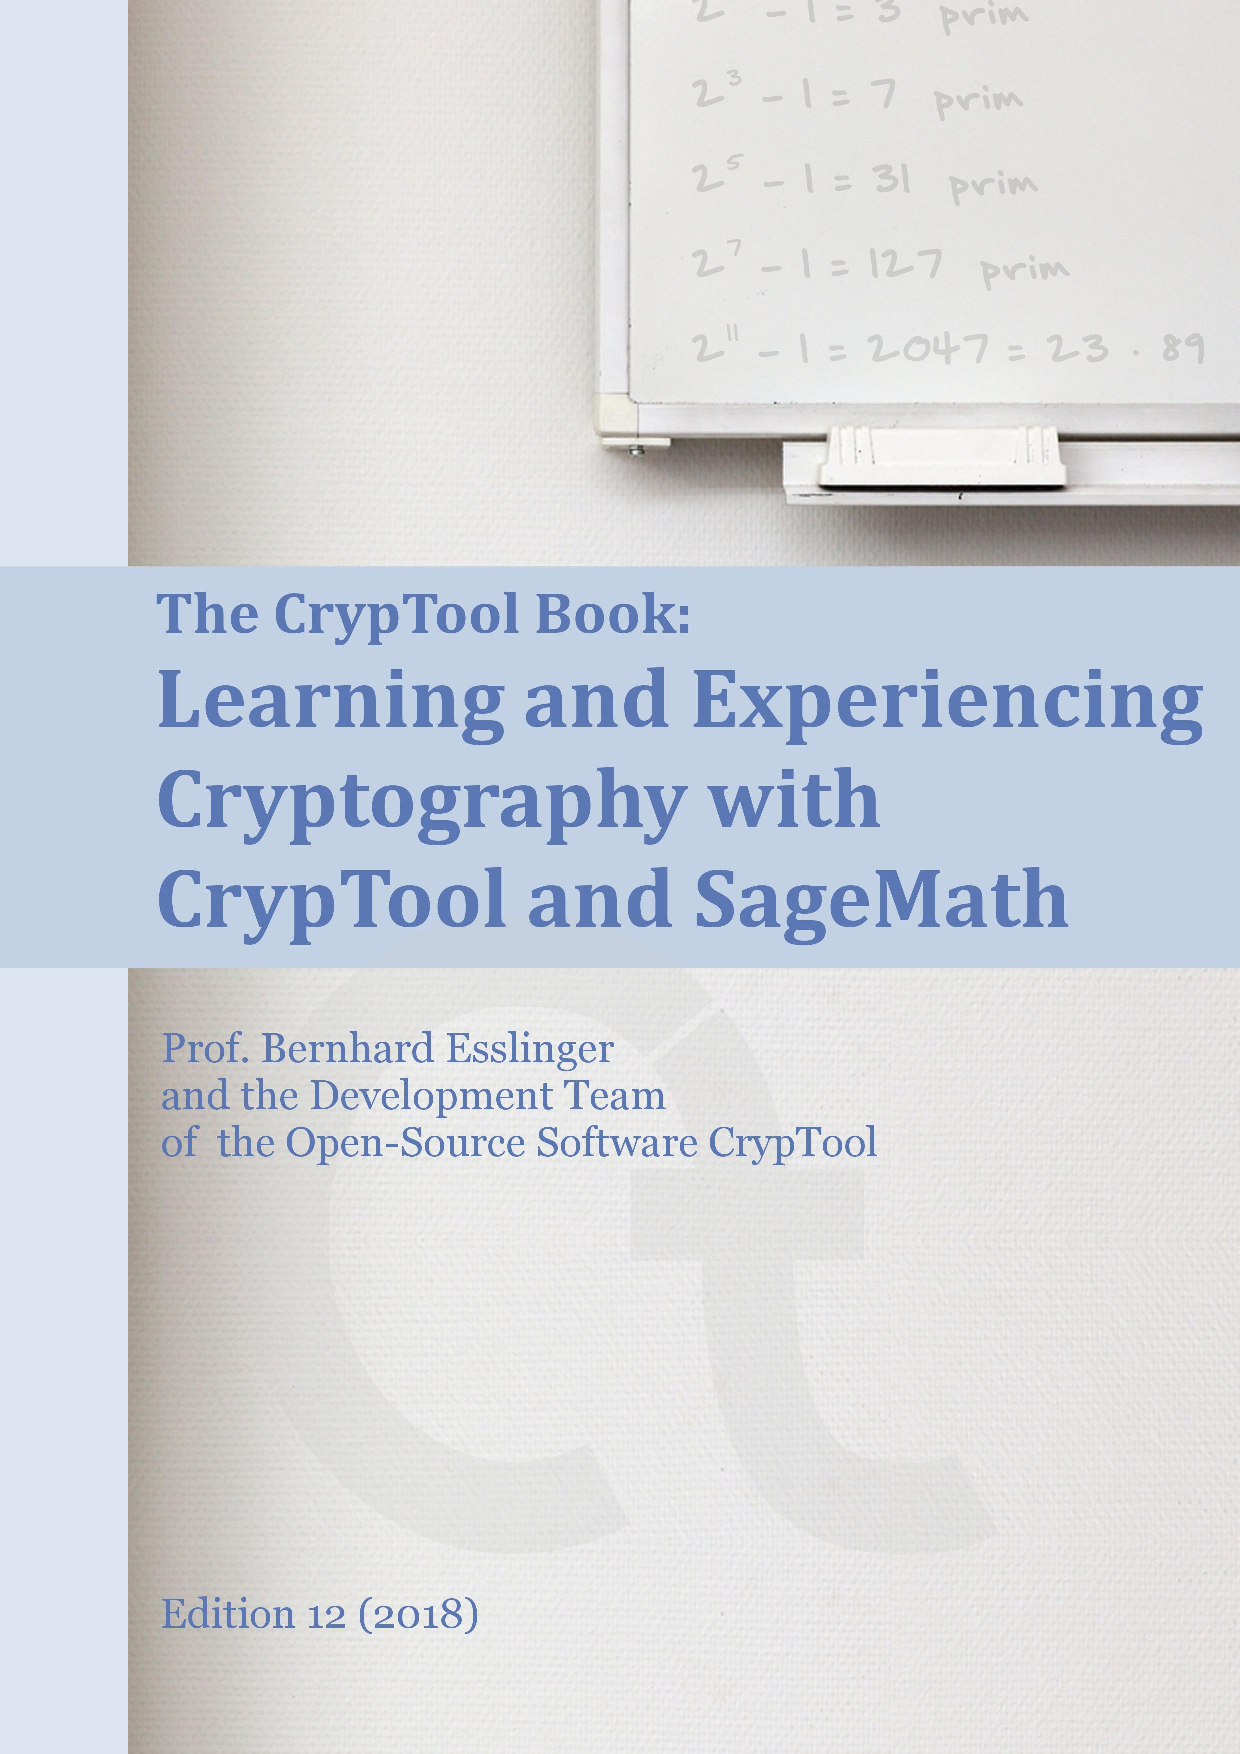
\includepdf[pages=1]{figures/coverv1_en.pdf}

\pagestyle{plain}
\tikzset{ampersand replacement=\&} %DIF > %16xxxxxxxxxxxxxx

\setlength{\fboxrule}{.5mm}
\setlength{\fboxsep}{1.75mm}
\setlength{\footnotesep}{6pt}
\addtolength{\footskip}{8pt}

\VerbatimFootnotes
\renewcommand\footnoterule{%
  \vspace{2em}
  \hrule width .4\columnwidth
 \vspace{4pt}
}


\frontmatter
\maketitle


\begin{quote}
This is a free document, so the content of the document can
be copied and distributed, also for commercial purposes --- as long as
the authors, title and the CrypTool web site (\url{www.cryptool.org})
are acknowledged. Naturally, citations from the CrypTool book are
possible, as in all other documents.\\
Additionally, this document is liable to the specific license of the
GNU Free Documentation Licence.

    Copyright \copyright{} 1998--2017 Bernhard Esslinger and the
    CrypTool Team. Permission is granted to copy,
    distribute and/or modify this document under the terms of the GNU
    Free Documentation License, Version 1.3 or any later version
    published by the Free Software Foundation. A copy of
    the license is included in the section entitled
    \hyperlink{appendix-GNU-fdl}{``GNU Free Documentation License''}.

    This also includes the code of the SageMath samples in this document.
\end{quote}


\vspace{70pt}\noindent Suggestion for referencing with bibtex:
\begin{Verbatim}%
[fontsize=\footnotesize]
@book{Esslinger:ctb_2017,
  editor    = {Bernhard Esslinger},
  title     = {{L}earning and {E}xperiencing {C}ryptography
               with {C}ryp{T}ool and {S}age{M}ath},
  publisher = {CrypTool Project},
  edition   = {12},
  year      = {2017}
}
\end{Verbatim}


\vspace{250pt}
\noindent
Source cover photograph: \url{www.photocase.com}, Andre Guenther\\
Typesetting software: \LaTeX\\
Version control software: Subversion


% $Id: aboutcryptool.tex 3714 2016-04-08 18:34:16Z esslinger $
% !Mode:: "TeX:DE"    % Setting document mode and submode for WinEdt
% ............................................................................
%          Ü b e r b l i c k  (Text der 4. Seite, noch bevor Content)
%
% ~~~~~~~~~~~~~~~~~~~~~~~~~~~~~~~~~~~~~~~~~~~~~~~~~~~~~~~~~~~~~~~~~~~~~~~~~~~~

\clearpage
\setcounter{secnumdepth}{-1}  % Prevent this chapter title from having a number
\chapter%[Überblick]%
{Überblick über den Inhalt des CrypTool-Buchs}
\setcounter{secnumdepth}{4}  % Set back default from CT-Book-de.tex (show numbers till level 4)

\parskip 4pt
%\vskip +12 pt
Der Erfolg des Internets hat zu einer verstärkten
Forschung der damit verbundenen Technologien geführt, was auch im
Bereich Kryptographie viele neue Erkenntnisse schaffte.

In diesem {\em Buch zu den CrypTool-Programmen} \index{CrypTool} finden Sie
eher mathematisch orientierte Informationen zum Einsatz von
kryptographischen Verfahren. Zu einigen Verfahren gibt es Beispielcode,
geschrieben für das Computer-Algebra-System \textbf{SageMath}\index{SageMath}
(siehe Anhang~\ref{s:appendix-using-sage}).
Die Hauptkapitel sind von verschiedenen \textbf{Autoren} verfasst
(siehe Anhang~\ref{s:appendix-authors}) %\hyperlink{appendix-authors}{Autoren}
und in sich abgeschlossen. Am Ende der meisten Kapitel finden Sie
Literaturangaben und Web-Links.
Die Kapitel wurden reichlich mit {\em Fußnoten} versehen, in denen auch darauf
verwiesen wird, wie man die beschriebenen Funktionen in den verschiedenen
CrypTool-Programmen aufruft.

Das \hyperlink{Chapter_EncryptionSecDefinitions}{erste Kapitel} beschreibt
die Prinzipien der symmetrischen und asymmetrischen
\hyperlink{Chapter_EncryptionSecDefinitions}{\textbf{Verschlüsselung}} und
gibt Definitionen für deren Widerstandsfähigkeit.

Im \hyperlink{Chapter_PaperandPencil}{zweiten Kapitel} wird -- aus
didaktischen Gründen -- eine ausführliche Übersicht
über \hyperlink{Chapter_PaperandPencil}\textbf{Papier- und Bleistiftverfahren}
gegeben.

Ein großer Teil des Buchs ist dem faszinierenden Thema der
\hyperlink{Chapter_Primes}\textbf{Primzahlen} (Kapitel \ref{Chapter_Primes})
gewidmet.
Anhand vieler Beispiele wird in die \hyperlink{Chapter_ElementaryNT}\textbf{modulare Arithmetik}
und die \hyperlink{Chapter_ElementaryNT}\textbf{elementare Zahlentheorie}
(Kapitel \ref{Chapter_ElementaryNT}) eingeführt. Hier bilden die Eigenschaften
des \textbf{RSA-Verfahrens} einen Schwerpunkt.

Danach erhalten Sie Einblicke in die mathematischen Konzepte und
Ideen hinter der \hyperlink{Chapter_ModernCryptography}{\textbf{modernen Kryptographie}}
(Kapitel \ref{Chapter_ModernCryptography}).

%Ein \hyperlink{Chapter_Hashes-and-Digital-Signatures}{weiteres Kapitel}
Kapitel \ref{Chapter_Hashes-and-Digital-Signatures} gibt einen Überblick zum Stand der
Attacken gegen moderne \hyperlink{Chapter_Hashes-and-Digital-Signatures}\textbf{Hashalgorithmen}
und widmet sich dann kurz den \hyperlink{Chapter_Hashes-and-Digital-Signatures}\textbf{digitalen Signaturen}
--- sie sind unverzichtbarer Bestandteil von E-Business-Anwendungen.

Kapitel \ref{Chapter_EllipticCurves} stellt \hyperlink{Chapter_EllipticCurves}
\textbf{Elliptische Kurven} vor: Sie sind eine Alternative zu RSA und für die
Implementierung auf Chipkarten besonders gut geeignet.

Kapitel \ref{Chapter_BitCiphers} führt in die \hyperlink{Chapter_BitCiphers}\textbf{Boolesche Algebra} ein.
Boolesche Algebra ist Grundlage der meisten modernen, symmetrischen
Verschlüsselungsverfahren, da diese auf Bitströmen und Bitblöcken operieren.
Prinzipielle Konstruktionsmethoden dieser Verfahren werden beschrieben
und in SageMath implementiert.

Kapitel \ref{Chapter_HomomorphicCiphers} stellt
\hyperlink{Chapter_HomomorphicCiphers}\textbf{Homomorphe Kryptofunktionen}
vor: Sie sind ein modernes Forschungsgebiet, das insbesondere im Zuge des
Cloud-Computing an Bedeutung gewann.

Kapitel \ref{Chapter_Dlog-FactoringDead} beschreibt
\hyperlink{Chapter_Dlog-FactoringDead}\textbf{Aktuelle
Resultate zum Lösen diskreter Logarithmen und zur Faktorisierung}.
Es gibt einen breiten Überblick und Vergleich über die zur Zeit besten
Algorithmen für (a) das Berechnen diskreter Logarithmen in
verschiedenen Gruppen, für (b) das Faktorisierungsproblem und
für (c) Elliptische Kurven. Dieser Überblick wurde zusammengestellt,
nachdem ein provozierender Vortrag auf der Black Hat-Konferenz
2013 für Verunsicherung sorgte, weil er die Fortschritte bei endlichen
Körpern mit kleiner Charakteristik fälschlicherweise auf Körper
extrapolierte, die in der Realität verwendet werden.

Das \hyperlink{Chapter_Crypto2020}{letzte Kapitel}
\hyperlink{Chapter_Crypto2020}\textbf{Krypto 2020}
diskutiert Bedrohungen für bestehende kryptographische Verfahren und
stellt alternative Forschungsansätze (Post-Quantum-Kryptographie)
für eine langfristige kryptographische Sicherheit vor.

Während die CrypTool-\textit{eLearning-Programme}\index{eLearning} eher den
praktischen Umgang motivieren und vermitteln, dient das \textit{Buch} dazu,
dem an Kryptographie Interessierten ein tieferes Verständnis für die
implementierten mathematischen Algorithmen zu vermitteln -- und das
didaktisch mög"-lichst gut nachvollziehbar.

Die \hyperlink{appendix-start}\textbf{Anhänge}
\ref{s:appendix-menu-overview-CT1},
\ref{s:appendix-template-overview-CT2},
\ref{s:appendix-function-overview-JCT} und
\ref{s:appendix-function-overview-CTO}
erlauben einen schnellen Überblick über die Funktionen in den verschiedenen
CrypTool-Varianten\index{CT1}\index{CT2}\index{JCT}\index{CTO} via:
\begin{itemize}
  \item der Funktionsliste und
        dem \hyperlink{appendix-menu-overview-CT1}
                      {Menübaum von CrypTool~1 (CT1)},
  \item der Funktionsliste und
        den \hyperlink{appendix-template-overview-CT2}
                      {Vorlagen in CrypTool~2 (CT2)},
  \item der \hyperlink{appendix-function-overview-JCT}
                      {Funktionsliste von JCrypTool (JCT)}, und
  \item der \hyperlink{appendix-function-overview-CTO}
                      {Funktionsliste von CrypTool-Online (CTO)}.
\end{itemize}
%Anker sind \hypertarget{appendix-menutree}{} und \label{s:appendix-menutree}
%  - \hyperlink{}{} legt Link auf die Seite unter den Text in 2. Klammer
%  - \ref{} legt Link und fügt Kapitelnummer ein.

% Bernhard Esslinger, Matthias Büger, Bartol Filipovic, Henrik Koy, Roger Oyono
% und Jörg Cornelius Schneider
Die Autoren möchten sich an dieser Stelle bedanken bei den Kollegen
in der jeweiligen Firma und an den Universitäten Bochum, Darmstadt, Frankfurt,
Gießen, Karlsruhe, Lausanne, Paris und Siegen.

\enlargethispage{0.5cm}
Wie auch bei dem E-Learning-Programm CrypTool\index{CrypTool} wächst
die Qualität des Buchs mit den Anregungen und Verbesserungsvorschlägen
von Ihnen als Leser. Wir freuen uns über Ihre Rück"-mel"-dung.



% Local Variables:
% TeX-master: "../script-de.tex"
% End:



\newpage
\pdfbookmark[0]{Contents Overview}{ShortContents}
\shorttoc{Contents Overview}{0}
\clearpage\phantomsection
\pdfbookmark[0]{\contentsname}{Contents}
\tableofcontents 

\newpage
\normalsize

\newcounter{mycounterDefaultParskip}
\setcounter{mycounterDefaultParskip}{4}
\parskip \value{mycounterDefaultParskip} pt 


\renewcommand{\bibname}{Bibliography \CTBChapName{}}
\newcommand{\CTBChapName}{(Chap Intro)}           % $Id$
% ............................................................................
%      V O R W O R T  und  E I N F � H R U N G (Zusammenspiel Skript-CT) 
% ~~~~~~~~~~~~~~~~~~~~~~~~~~~~~~~~~~~~~~~~~~~~~~~~~~~~~~~~~~~~~~~~~~~~~~~~~~~~


% --------------------------------------------------------------------------
\clearpage\phantomsection
\addcontentsline{toc}{chapter}{Preface to the 10th Edition of the CrypTool Script}
\chapter*{Preface to the 10th Edition of the CrypTool Script}

Starting in the year 2000 this script became part of the 
CrypTool v1\index{CrypTool 1.x} package. It is designed to accompany the program 
CrypTool by explaining some mathematical topics in more detail, 
but still in a way which is easy to understand.

In order to also enable developers/authors to work together independently 
the topics have been split up and for each topic an extra chapter has been 
written which can be read on its own. The later editorial work in TeX added 
cross linkages between different sections and footnotes describing where you
can find the according functions within the CrypTool v1\index{CrypTool 1.x} 
program \hyperlink{appendix-menutree}{(see menu tree} in appendix \ref{s:appendix-menutree}).
% \hypertarget{appendix-menutree}{}\label{s:appendix-menutree}
Naturally there are many more interesting topics in mathematics and
cryptography which could be discussed in greater depth -- therefore this
is only one of many ways to do it.

The rapid spread of the Internet has also lead to intensified research in the
technologies involved, especially within the area of cryptography where a good
deal of new knowledge has arisen.

%This edition of the script adds some topics, but mainly updates areas (e.g. the
%summaries of topical research areas):
This edition completely updated the TeX sources of the document, and of course
the content of the script was corrected, amended and updated with some topics, e.g.:
\vspace{-7pt}
\begin{itemize}
  \item the search for the largest prime numbers 
        (chap. \ref{search_for_very_big_primes}), 
  \item progress in cryptanalysis of hash algorithms 
        (chap. \ref{NeueAES-Analyse}) and
%  \item progress in cryptanalysis of hash algorithms 
%        (chap. \ref{collision-attacks-against-sha-1}) and
%  \item progress in ideas for new crypto methods (RSA successor) 
%        (chap. \ref{xxxxxxxxxBrute-force-gegen-Symmetr})\index{xxxxxxxxxxxxxxxx} and
  \item the list of movies or novels, in which cryptography or number theory 
        played major role (see appendix \ref{s:appendix-movies});
        and where primes are used as hangers  
        (see curiouses in \ref{HT-Quaint-curious-Primes-usage}).
\end{itemize}

Newly added is the appendix \ref{s:appendix-using-sage} about using the
computer algebra system Sage. This was added because Sage becomes
more and more the standard open-source CAS system. Accordingly all
samples written before in Pari-GP and Mathematica have been substituted
with Sage code. Thanks to Minh Van Nguyen, a lot of new code samples could be added.

The first time the document was delivered with CrypTool\index{CrypTool} 
was in version 1.2.01. Since then it has been expanded and revised in almost
every new version of CrypTool.

I am deeply grateful to all the people helping with their impressive
commitment who have made this global project so successful.
Thanks also to the readers who sent us feedback.
% Especially I would like to acknowledge the English language proof-reading
% of this script version done by Richard Christensen and Lowell Montgomery.

I hope that many readers have fun with this script and that they get 
out of it more interest and greater understanding of this modern but 
also very ancient topic.
\\
\\
% [1.5\baselineskip]
% \enlargethispage*{2\baselineskip}
% \nopagebreak
Bernhard Esslinger
\\
\\
% [\baselineskip]
Frankfurt (Germany), August 2009



% --------------------------------------------------------------------------
\clearpage\phantomsection
\addcontentsline{toc}{chapter}{Introduction -- How do the Script and the Program Play together?}
\chapter*{Introduction -- How do the Script and the Program Play together?}

\textbf{This script}

This document is delivered together with the open-source program CrypTool\index{CrypTool}.

The articles in this script are largely self-contained and
can also be read independently of CrypTool\index{CrypTool}.

Chapters  \ref{Chapter_ModernCryptography} (Modern Cryptography) and 
\ref{Chapter_EllipticCurves} (Elliptic Curves) require a deeper knowledge
in mathematics, while the other chapters should be understandable with a 
school leaving certificate.

The \hyperlink{appendix-authors}{authors}
have attempted to describe cryptography for a broad 
audience -- without being mathematically incorrect. We believe that this
didactic pretension is the best way to promote the awareness for IT
security and the readiness to use standardized modern cryptography.
\par \vskip + 15pt


\noindent \textbf{The program CrypTool\index{CrypTool}}

CrypTool\index{CrypTool} is an educational program with a comprehensive online
help enabling you to use and analyse cryptographic procedures within a
unified graphical user interface.

CrypTool\index{CrypTool} is used world-wide for 
training in companies and teaching at schools and universities worldwide, and
several universities are helping to further develop the project.
\par \vskip + 15pt


\noindent \textbf{Acknowledgment}

At this point I'd like to thank explicitly the following people who
particularly contributed to CrypTool\index{CrypTool}. They applied their
very special talents and showed really great engagement:
\vspace{-7pt}
%\begin{itemize}
\begin{list}{\textbullet}{\addtolength{\itemsep}{-0.5\baselineskip}}
   \item Mr.\ Henrik Koy
   \item Mr.\ J\"org-Cornelius Schneider
   \item Mr.\ Florian Marchal
   \item Dr.\ Peer Wichmann
   \item Staff of Prof.\ Claudia Eckert, Prof.\ Johannes Buchmann and Prof.\ Torben Weis.
\end{list}
%\end{itemize}
Also I want to thank all the many people not mentioned here for their 
hard work (mostly carried out in their spare time).
\\
\\
Bernhard Esslinger
\\
\\
Frankfurt (Germany), July 2009

% Local Variables:
% TeX-master: "../script-en.tex"
% End:

\mainmatter
\renewcommand{\CTBChapName}{(Chap CryptoMeth)}    % ..............................................................................
%                V E R S C H L U E S S E L U N G S V E R F A H R E N
% ~~~~~~~~~~~~~~~~~~~~~~~~~~~~~~~~~~~~~~~~~~~~~~~~~~~~~~~~~~~~~~~~~~~~~~~~~~~~~~

\newpage
\section{Encryption procedures}
\hypertarget{Kapitel_1}{}
(Bernhard Esslinger, besslinger@web.de, May 1999, Updates Dec. 2001, Feb. 2003)


% --------------------------------------------------------------------------
\subsection{Encryption}

The purpose of encryption \index{Encryption} is to change data in such a way
that only an authorised recipient is able to reconstruct the plaintext. This has
the advantage that you can transmit encrypted data openly and nevertheless need
not fear a perpetrator reading the data without authorisation. Authorised
recipients possess a piece of secret information --- called the key --- which
allows them to decrypt the data while it remains hidden from everyone else.\par \vskip + 3pt

One encryption procedure has been proved to be secure --- the {\em One Time
  Pad}.
\index{One �Time �Pad} However, this procedure has several practical
disadvantages (the key used must be selected randomly and must be just as long
as the message to be protected), which means that it is hardly used except in
closed environments such as for the hot wire between Moscow and Washington.\par \vskip + 3pt

For all other procedures there is a (theoretical) possibility of breaking them.
If the procedures are good, however, the time taken to break them is so long
that it is practically impossible to do and these procedures can therefore be
considered (practically) secure.\par \vskip + 3pt

We basically distinguish between symmetric and asymmetric encryption procedures.

% --------------------------------------------------------------------------
\subsubsection[Symmetric encryption]
{Symmetric encryption\footnotemark}
\footnotetext{%
With CrypTool\index{CrypTool} v1.3 you can execute the following modern
symmetric encryption algorithms 
(using the menu ``Crypt \textbackslash Symmetric''): \\
IDEA, RC2, RC4, DES (ECB), DES�(CBC), Triple-DES�(ECB), Triple-DES�(CBC),
MARS (AES candidate), RC6 (AES candidate), Serpent (AES candidate), 
Twofish (AES candidate), Rijndael (official AES algorithm).
}

For {\em symmetric} encryption \index{Encryption!symmetric} the sender and
recipient must possess a common (secret) key which they have exchanged before
actually starting to communicate. The sender uses this key to encrypt the
message and the recipient uses it to decrypt it.\par \vskip + 3pt

The advantages of symmetric algorithms are the high speed with which data can be
encrypted and decrypted. One disadvantage is the need for key management. In
order to communicate with one another confidentially, sender and recipient must
have exchanged a key using a secure channel before actually starting to
communicate. Spontaneous communication between individuals who have never met
therefore seems virtually impossible. If everyone wants to communicate with
everyone else spontaneously at any time in a network of $ n $ subscribers, each
subscriber must have previously exchanged a key with each of the other $n-� 1$
subscribers. A total of $n(n - 1)/2$ keys must therefore be exchanged.\par \vskip + 3pt

The most well-known symmetric encryption procedure is the \index{DES} DES-algorithm. The DES-algorithm has been developed by IBM in collaboration with the
National Security Agency \index{NSA} (NSA), and was published as a standard in
1975. Despite the fact that the procedure is relatively old, no effective attack
on it has yet been detected. The most effective way of attacking consists of
testing all possible keys until the right one is found ({\em brute-force-attack}).
\index{Attack!brute-force} Due to the relatively short key length of
effectively 56 bits (64 bits, which however include 8 parity bits), numerous
messages encrypted using DES have in the past been broken. Therefore, the
procedure can now only be considered to be conditionally secure. Symmetric
alternatives to the DES procedure include the IDEA \index{IDEA} or Triple DES
algorithms.\par \vskip + 3pt

Up-to-the-minute procedures are the symmetric AES procedures. The associated
Rijndael procedure was declared winner the AES award on 2 October 2000 and thus
succeeds the DES procedure.

More details about the AES algorithms can be found within the Online help of CrypTool\index{CrypTool} (in the index see head-word {\em AES} and then the help pages {\em AES candidates}, {\em The AES Winner Rijndael} and {\em The Rijndael encryption algorithm}).


% --------------------------------------------------------------------------
\subsubsection{New results about cryptanalysis of AES}

Below you will find some results, which have recently called into question the security of the AES algorithm -- from our point of view these doubts practically still remain unfounded. The following information is based on the original papers and the articles \cite{Wobst-iX2002} and \cite{Lucks-DuD2002}.

AES with a minimum key length of 128 bit is still in the long run sufficiently secure against brute-force attacks - as long as the quantum computers weren't powerful enough. When announced as new standard AES was immune against all known crypto attacks, mostly based on statistical considerations and earlier applied to DES: using pairs of clear and cipher texts expressions are constructed, which are not completely at random, so they allow conclusions to the used keys. These attacks required unrealistically large amounts of intercepted data.

Cryptanalysts already label methods as ``academic success'' or as ``cryptanalytic attack'' if they are theoretically faster than the complete testing of all keys (brute force analysis). In the case of AES with the maximal key length (256 bit) exhaustive key search on average needs $2^{255}$ encryption operations. A cryptanalytic attack needs to be better than this. At present between $2^{75}$ and $2^{90}$ encryption operations are estimated to be performable for organizations, for example a security agency.

In their 2001-paper Ferguson, Schroeppel and Whiting \cite{Ferguson2001} presented a new method of symmetric codes cryptanalysis: They described AES with a closed formula (in the form of a continued fraction) which was possible because of the "relatively" clear structure of AES. This formula consists of around 1000 trillion terms of a sum - so it does not help concrete practical cryptanalysis. Nevertheless -curiosity in the academic community awakened. It was already known, that the 128-bit AES could be described as an over-determined system of about 8000 quadratic equations (over an algebraic number field) with about 1600 variables (some of them are the bits of the wanted key) -- equation systems of that size are in practice not solvable. This special equation system is relatively sparse, so only very few of the quadratic terms (there are about 1,280,000 are possible quadratic terms in total) appear in the equation system.

The mathematicians Courois and Pieprzyk \cite{Courtois2002} published a paper in 2002, which got a great deal of attention amongst the crypto community: The pair had further developed the XL-method (eXtended Linearization), introduced at Eurocrypt 2000 by Shamir et al., to create the so called XSL-method (eXtended Sparse Linearization). The XL-method is a heuristic technique, which in some cases manages to solve big non-linear equation systems and which was till then used to analyze an asymmetric algorithm (HFE).  The innovation of Courois and Pieprzyk was, to apply the XL-method on symmetric codes: the XSL-method can be applied to very specific equation systems. A 256-bit AES could be attacked in roughly $2^{230}$ steps. This is still a purely academic attack, but also a direction pointer for a complete class of block ciphers. The major problem with this attack is that until now nobody has worked out, under what conditions it is successful: the authors specify in their paper necessary conditions, but it is not known, which conditions are sufficient.
There are two very new aspects of this attack: firstly this attack is not based on statistics but on algebra. So attacks seem to be possible, where only very small amounts of cipher text are available. Secondly the security of a product-algorithm does not exponentially increase with the number of rounds.

Currently there is a large amount of research in this area: for example Murphy and Robshaw presented a paper at Crypto 2002 \cite{Robshaw2002a}, which could dramatically improve cryptanalysis: the burden for a 128-bit key was estimated at about $2^{100}$ steps by describing AES as a special case of an algorithm called BES (Big Encryption System), which has an especially "round" structure. But even $2^{100}$ steps are beyond what is achievable in the foreseeable future. Using a 256 bit key the authors estimate that a XSL-attack will require $2^{200}$ operations.

More details can be found at: \\
\href{http://www.cryptosystem.net/aes}{\texttt{http://www.cryptosystem.net/aes}} and \\ 
\href{http://www.minrank.org/aes/}{\texttt{http://www.minrank.org/aes/}}

So for 256-AES the attack is much more effective than brute-force but still far away from any computing power which could be accessible in the short-to-long term. The discussion is very controversial: Don Coppersmith (one of the inventors of DES) for example queries the practicability of the attack because XLS would provide no solution for AES \cite{Coppersmith2002}. This concludes that then the optimization of Murphy and Robshaw \cite{Robshaw2002b} would not work.


% --------------------------------------------------------------------------
\subsubsection{Asymmetric encryption}

In the case of {\em asymmetric} encryption \index{Encryption!asymmetric} each
subscriber has a personal pair of keys consisting of a {\em secret}
\index{Key!secret} key and a {\em public} key\index{Key!public}. The public
key, as its name implies, is made public, e.g. in a key directory on the
Internet.\par \vskip + 3pt

If Alice wants to communicate with Bob, then she finds Bob's public key 
in the directory and uses it to encrypt her message to him. She then sends
this cipher text to Bob, who is then able to decrypt it again using his 
secret key. As only Bob knows his secret key, only he can decrypt 
messages addressed to him.
Even Alice who sends the message cannot restore plaintext from the (encrypted)
message she has sent. Of course, you must first ensure that the public key
cannot be used to derive the private key.\par \vskip + 3pt

Such a procedure can be demonstrated using a series of thief-proof letter boxes.
If I have composed a message, I then look for the letter box of the recipient
and post the letter through it. After that, I can no longer read or change the
message myself, because only the legitimate recipient possesses the key for the
letter box.\par \vskip + 3pt

The advantage of asymmetric procedures is the easy \index{Key management} key management. Let's look again at a network with $n$
subscribers. In order to ensure that each subscriber can establish
an encrypted connection to each other subscriber, each subscriber
must possess a pair of keys. We therefore need $2n$ keys or $n$
pairs of keys. Furthermore, no secure channel is needed before
messages are transmitted, because all the information required in
order to communicate confidentially can be transmitted openly. In
this case, you simply have to pay attention to the accuracy
(integrity and authenticity) \index{Authenticity} of the public
key. Disadvantage: Pure asymmetric procedures take a lot longer to
perform than symmetric ones.\par \vskip + 3pt

The most well-known asymmetric procedure is the \index{RSA} RSA algorithm,
named after its developers Ronald \index{Rivest Ronald} Rivest, Adi
\index{Shamir Adi} Shamir and Leonard \index{Adleman Leonard} Adleman. The RSA algorithm
was published in 1978. The concept of asymmetric encryption was first
introduced by Whitfield Diffie \index{Diffie Whitfield}  and Martin
\index{Hellman Martin} Hellman in 1976. Today, the ElGamal \index{ElGamal}
procedures also play a decisive role, particularly the \index{Schnorr} Schnorr
variant in the \index{DSA} DSA (Digital \index{Signatures!digital}Signature
Algorithm).


% --------------------------------------------------------------------------
\newpage
\subsubsection[Hybrid procedures]
{Hybrid procedures\footnotemark}
\footnotetext{%
Within CrypTool\index{CrypTool} v1.3 you can get a visualization of this
technique using the menu ``Crypt \textbackslash Hybrid Demonstration'': 
this dialogue shows the single steps and its dependencies with concrete
numbers.
}\index{Hybrid procedures}

In order to benefit from the advantages of symmetric and asymmetric techniques
together, hybrid procedures are usually used (for encryption) in practice.
\par \vskip + 3pt

In this case the data is encrypted using symmetric procedures: the key is a
session key\index{Session key} generated by the sender randomly that is only used for this message.
This session key is then encrypted using the asymmetric procedure and
transmitted to the recipient together with the message. Recipients can determine
the session key using their secret keys and then use the session key to encrypt
the message. In this way, we can benefit from the easy key management
\index{Key management} of asymmetric procedures and encrypt large quantities of data
quickly and efficiently using symmetric procedures.


% --------------------------------------------------------------------------
\subsubsection{Further details}

Beside information you can find in many books and on a lot of websites the 
online help of CrypTool\index{CrypTool} also offers very many details about
the symmetric and asymmetric encryption methods.


% --------------------------------------------------------------------------
\begin{thebibliography}{99999}
\addcontentsline{toc}{subsection}{Bibliography}

\bibitem[Schmeh2003]{Schmeh2003}  \index{Schmeh 2003}
        Klaus Schmeh, \\
        {\em Cryptography and Public Key Infrastructures on the Internet}, 
	John Wiley \& Sons Ltd., Chichester 2003. \\
        A considerable, up-to-date, good reading book, which also 
	considers practical problems, like standardisation or
        real existing software.


\bibitem[Coppersmith2002]{Coppersmith2002}  \index{Coppersmith 2002}
        Don Coppersmith, \\
        {\em Re: Impact of Courtois and Pieprzyk results}, 
	2002-09-19, AES Discussion Groups at \\
        \href{http://aes.nist.gov/aes/}
        {\texttt{http://aes.nist.gov/aes/}}

\bibitem[Courtois2002]{Courtois2002}  \index{Courtois 2002}
        Nicolas Courtois, Josef Pieprzyk, \\
        {\em Cryptanalysis of Block Ciphers with Overdefined Systems of Equations}, 
	received 10 Apr 2002, last revised 9 Nov 2002,
	A different version, so called compact version of the first XSL attack,
	was published in Asiacrypt Dec 2002, \\
        \href{http://eprint.iacr.org/2002/044}
        {\texttt{http://eprint.iacr.org/2002/044}}

\bibitem[Ferguson2001]{Ferguson2001}  \index{Ferguson 2001}
        Niels Ferguson, Richard Schroeppel, Doug Whiting, \\
        {\em A simple algebraic representation of Rijndael}, 
	Draft 2001/05/1, \\
        \href{http://www.xs4all.nl/~vorpal/pubs/rdalgeq.html}
        {\texttt{http://www.xs4all.nl/\~{}vorpal/pubs/rdalgeq.html}}

\bibitem[Lucks-DuD2002]{Lucks-DuD2002}  \index{Lucks 2002}
        Stefan Lucks, R"udiger Weis, \\
        {\em Neue Ergebnisse zur Sicherheit des Verschl�sselungsstandards AES}, 
	in DuD Dec. 2002.

\bibitem[Robshaw2002a]{Robshaw2002a}  \index{Robshaw 2002}
        S.P. Murphy, M.J.B. Robshaw, \\
        {\em Essential Algebraic Structure within the AES}, 
	June 5, 2002, Crypto 2002,  \\
        \href{http://www.isg.rhul.ac.uk/\~{}mrobshaw/rijndael/rijndael.html}
        {\texttt{http://www.isg.rhul.ac.uk/~mrobshaw/rijndael/rijndael.html}}

\bibitem[Robshaw2002b]{Robshaw2002b}  \index{Robshaw 2002}
        S.P. Murphy, M.J.B. Robshaw, \\
        {\em Comments on the Security of the AES and the XSL Technique}, 
	September 26, 2002, \\
        \href{http://www.isg.rhul.ac.uk/\~{}mrobshaw/rijndael/rijndael.html}
        {\texttt{http://www.isg.rhul.ac.uk/~mrobshaw/rijndael/rijndael.html}}

\bibitem[Wobst-iX2002]{Wobst-iX2002}  \index{Wobst 2002}
        Reinhard Wobst, \\
        {\em Angekratzt - Kryptoanalyse von AES schreitet voran}, 
	in iX Dec. 2002, \\
	plus the reader's remark by Johannes Merkle in iX Feb. 2003.

\end{thebibliography}


% Local Variables:
% TeX-master: "../script-en.tex"
% End:

\renewcommand{\CTBChapName}{(Chap PaP)}           % $Id$
% ..............................................................................
%                V E R S C H L U E S S E L U N G S V E R F A H R E N
%
% Writing rule: Capitel header with all nouns/verbs-words capitalized,
%               All other headers in the normal lower/upper case manner
%               like sentences (without a dot at the end).
% Writing rule: Use American English instead of British English consistently.
%
% ~~~~~~~~~~~~~~~~~~~~~~~~~~~~~~~~~~~~~~~~~~~~~~~~~~~~~~~~~~~~~~~~~~~~~~~~~~~~~~
%------------------------------------------------------------------------------
% First Editor: Christine St�tzel, April 2004
% Update and corrections: B. Esslinger, June 2005
% Update and corrections: B. Esslinger, June 2005
% Update B. Esslinger and Minh Van Nguyen, July 2009 
%------------------------------------------------------------------------------

% ``primenet''
\newpage
\hypertarget{Kapitel_PaperandPencil}{}

\chapter{Paper and Pencil Encryption Methods}
\label{Kapitel_PaperandPencil}
(Christine St\"otzel, April 2004; Updates: B.+C. Esslinger, June 2005; Updates Minh Van Nguyen and B. Esslinger, July 2009)
\index{Paper and pencil methods}

\begin{center}
\fbox{\parbox{15cm}{%
{\em Edgar Allan Poe\index{Poe, Edgar Allan}: 
A Few Words on Secret Writing, 1841}\\
Few persons can be made to believe that it is not quite an easy thing
to invent a method of secret writing which shall baffle investigation.
Yet it may be roundly asserted that human ingenuity cannot concoct a
cipher which human ingenuity cannot resolve.}}
\end{center}

The following chapter provides a broad overview of paper and pencil 
methods\footnote{%
The footnotes to this chapter describe how the methods can be
performed using CrypTool CrypTool 1.
Additionally the last sub chapter (\ref{PaP_Sage_samples})
contains example code using the computer algebra system Sage\index{Sage}.
                 }
each with references to deeper information.
All techniques that people can apply manually to en- and decipher a message are 
embraced by this term. These methods were and still are especially popular with
secret services, as a writing pad and a pencil -- in contrast to electronic
aids -- are totally unsuspicious.

The first paper and pencil methods already arose about 3000 years ago, but new
procedures were developed during the past century, too. All paper and pencil 
methods are a matter of symmetric methods\index{Encryption!symmetric}. 
Even the earliest encryption algorithms use the basic principles such as 
transposition, substitution, block construction and their combinations. 
Hence it is worthwhile to closely consider this ``ancient'' methods especially
under didactic aspects.

Methods to be successful and wide-spread had to fulfill some attributes which are equally required for modern algorithms:
\begin{itemize}
\item Exhaustive description, almost standardization (including special cases,
      padding, etc.).
\item Good balance between security and usability 
      (because methods being too complicated were error-prone or
      unacceptably slow).
\end{itemize}


\newpage
%------------------------------------------------------------------------------
\section{Transposition ciphers}
\label{PaP_transposition_ciphers}
\index{Transposition}

Encrypting a message by means of transposition\index{Transposition} does not 
change the original characters of this message, only their order is modified
(transposition = exchange)\footnote{Another name used for transposition is
permutation\index{Permutation}.}.

%------------------------------------------------------------------------------
\subsection{Introductory samples of different transposition ciphers}
\label{introsamplesTranspositionCiphers}

\begin{itemize}

\item {\bf Rail Fence}\footnote{%
   This method can directly be found in CrypTool\index{CrypTool} at the menu item
   {\bf Crypt/Decrypt \textbackslash{} Symmetric (classic) \textbackslash{} Scytale / Rail Fence}.
   You can simulate this method also under the menu {\bf Crypt/Decrypt \textbackslash{} 
   Symmetric (classic) \textbackslash{} Permutation}: For a Rail Fence with
   2 lines use as key ``B,A'' and accept the default settings (only one
   permutation, where your input is done line-by-line and the output is
   taken column-by-column). 
   Using the key ``A,B'' would start the zigzag pattern below in the
   way, that the first letter is written into the first line instead of the
   second line.}
   \cite{pp:Singh2001}\index{Rail Fence cipher}:
   The characters of a message are alternately written in two (or more) lines,
   creating a zigzag pattern. The resulting ciphertext is read out 
   line by line.\\
   This is more a children's method.

   Plaintext\footnote{If the alphabet only uses 26 letters, we write the
   plaintext in small letters and the ciphertext in capital letters.}%
   : an example of transposition

\begin{table}[ht]
\begin{center}
\begin{tabular}{r@{\:}r@{\:}r@{\:}r@{\:}r@{\:}r@{\:}r@{\:}r@{\:}r@{\:}r@{\:}r@{\:}r@{\:}r@{\:}r@{\:}r@{\:}r@{\:}r@{\:}r@{\:}r@{\:}r@{\:}r@{\:}r@{\:}r@{\:}r@{\:}}
	  & n &   & x &   & m &   & l &   & o &   & t &   & a &   & s &   & o &   & i &   & i &   & n \\
	a &   & e &   & a &   & p &   & e &   & f &   & r &   & n &   & p &   & s &   & t &   & o &   \\
\end{tabular}
\caption{Rail Fence cipher}
\end{center} 
\end{table}

   Ciphertext\footnote{The letters of the cleartext are -- as used 
   historically -- grouped within blocks of 5 letters. It does not matter
   if the (constant) block length is different or no blank is inserted.}%
   : NXMLO TASOI INAEA PEFRN PSTO\\


\item {\bf Scytale}\footnote{%
   This method can directly be found in CrypTool\index{CrypTool} at the menu item
   {\bf Crypt/Decrypt \textbackslash{} Symmetric (classic) \textbackslash{} Scytale / Rail Fence}.
   As this method is a special case of a simple columnar transposition, you also can
   simulate it in CrypTool\index{CrypTool} under the 
   menu {\bf Crypt/Decrypt \textbackslash{} Symmetric (classic) \textbackslash{} 
   Permutation}: For the Scytale within the dialog box only the first 
   permutation is used. If the wood has e.g. 4 angles use as key ``1,2,3,4''.
   This is equivalent to write the text horizontally in blocks of 4 letters 
   in a matrix and to read it out vertically . 
   Because the key is in an in ascending order, the Scytale is denoted as
   an identical permutation. And because writing and read-out is done only
   once it is a simple (and no double) permutation.}
   \cite{pp:Singh2001}\index{Scytale}%
   : 
   This method was probably used since 600 B.C. -- a description
   of how it operated is not known from before Plutarch (50-120 B.C.).\\
   A long strip of paper is wrapped around a wooden cylinder and then the 
   message is written along the length of this strip. The ciphertext is 
   produced by unwinding the strip.

\item {\bf Grille} \cite{pp:Goebel2003}: Both parties use identical stencils. 
   Line by line, their holes are filled with plaintext that is read out 
   column by column to produce the ciphertext. If there is plaintext left, 
   the procedure is repeated\footnote{%
   This method cannot be simulated with a pure column transposition.}.

   \hypertarget{turning-grille}{}
\item {\bf Turning grille} \cite{pp:Savard1999}%
   \index{Turning grille}: 
   The German army used turning 
   grilles during WW1\footnote{The turning grille was already invented in 
   1881 by Eduard Fleissner von Wostrowitz.\\
   A good visualization can be found under www.turning-grille.com.}%
   . 
   A square grille serves as a stencil, a quarter of its fields being holes.
   The first part of the message is written on a piece of paper through	these
   holes, then the grille is rotated by 90 degrees and the user can
   write down the second part of the message, etc. But this method does only
   work, if the holes are chosen carefully: Every field has to be used, and
   no field may be used twice, either. The ciphertext is read out line by
   line.

   In the example for a turning grille in the following table you can write
   4 times 16 characters of the cleartext on a piece of paper:
\begin{table}[ht]
\begin{center}
\begin{tabular}{|cccc|cccc|}
\hline 	
	O & - & - & - & - & O & - & - \\
	- & - & - & O & O & - & - & O \\
	- & - & - & O & - & - & O & - \\
	- & - & O & - & - & - & - & - \\
\hline 	
	- & - & - & - & O & - & - & - \\
	O & - & O & - & - & - & O & - \\
	- & O & - & - & - & - & - & O \\
	- & - & - & O & O & - & - & - \\
\hline
\end{tabular}  
\caption{8x8 turning grille} 
\end{center}   
\end{table}

\end{itemize}


%------------------------------------------------------------------------------
% {\bf Column and row transposition}
\subsection[Column and row transposition ciphers]
    {Column and row transposition\footnotemark}
    \footnotetext{%
Most of the following methods can be simulated in CrypTool\index{CrypTool} 
under the menu {\bf Crypt/Decrypt \textbackslash{} Symmetric (classic) 
\textbackslash{} Permutation}.}

\begin{itemize}

\item {\bf Simple columnar transposition} \cite{pp:Savard1999}: First of all, 
   a keyword is chosen, that is written above the columns of a table. This
   table is filled with the text to be encrypted line by line. Then the 
   columns are rearranged by sorting the letters of the keyword alphabetically.
   Afterwards the columns are read out from left to right to build the 
   ciphertext\footnote{%
   Using CrypTool: Choose a key for the 1st permutation, input line by line, 
   permute and output column by column.}.

   Plaintext: an example of transposition

\begin{table}[ht]
\begin{center}
\begin{tabular}{|c|c|c|}
\hline 	
	K & E & Y \\
\hline
	a & n & e \\
	x & a & m \\
	p & l & e \\
	o & f & t \\
	r & a & n \\
	s & p & o \\
	s & i & t \\
	i & o & n \\
\hline
\end{tabular}
\caption{Simple columnar transposition}
\end{center} 
\end{table}

   Transposition key: K=2; E=1; Y=3. \\
   Ciphertext: NALFA PIOAX PORSS IEMET NOTN\\

\item {\bf AMSCO} \cite{pp:ACA2002}\index{AMSCO}: The characters of the plaintext
   are written in alternating groups of one respectively two letters into a
   grille. Then the columns are swapped and the text can be read out.

\item {\bf Double column transposition} \cite{pp:Savard1999}
   \index{Double column transposition}: 
   Double columnar transposition
   was frequently used during WW2 and during the Cold War. Two simple columnar
   transpositions with different keys are executed successively\footnote{%
   Using CrypTool: Choose a key for the 1st permutation, input line by line, 
   permute and output column by column. Then choose a (different) key for the
   2nd permutation, input line by line, permute and output column by column.}.
	
\item {\bf Column transposition, General Luigi Sacco} \cite{pp:Savard1999}: The 
   columns of a table are numbered according to the letters of the keyword. 
   The plaintext is entered line by line, in the first line up to column 
   number one, in the second line up to column number two, etc. 
   Again, the ciphertext is read out in columns.

   Plaintext: an example of transposition

\begin{table}[ht]
\begin{center}
\begin{tabular}{|c|c|c|c|c|c|}
\hline 	
	C & O & L & U & M & N\\
	1 & 5 & 2 & 6 & 3 & 4\\
\hline
	a &   &   &   &   &  \\
	n & e & x &   &   &  \\
	a & m & p & l & e &  \\
	o & f & t & r & a & n\\
	s & p &   &   &   &  \\
	o & s & i & t &   &  \\
	i & o & n &   &   &  \\
\hline
\end{tabular}
\caption{Columnar transposition (General Luigi Sacco)}
\end{center} 
\end{table}

   Ciphertext: ANAOS OIEMF PSOXP TINLR TEAN\\


\item {\bf Column transposition, French army in WW1} 
   \cite{pp:Savard1999}: 
   After executing a simple columnar transposition, diagonal rows are read out.


\item {\bf Row transposition} \cite{pp:Savard1999}: The plaintext is divided 
   into blocks of equal length and a keyword is chosen.
   Now the letters of the keyword are numbered and permutation is done only
   within each block according to this numbering\footnote{%
   Using CrypTool: Choose a key for 1st permutation, input line by line, 
   permute column by column and output line by line.}.

\end{itemize}



%------------------------------------------------------------------------------
\subsection{Further transposition algorithm ciphers}

\begin{itemize}

\item {\bf Geometric figures} \cite{pp:Goebel2003}: Write the message into a
   grille following one pattern and read it out using another.

\item {\bf Union Route Cipher} \cite{pp:Goebel2003}: The Union Route Cipher
   derives from Civil War. This method does not rearrange letters of a given
   plaintext, but whole words. Particularly sensitive names and terms are
   substituted by codewords which are recorded in codebooks together with
   the existing routes.
   A route determines the size of a grille and the pattern that is used to 
   read out the ciphertext. In addition, a number of filler words is defined.

\item {\bf Nihilist Transposition} \cite{pp:ACA2002}\index{Nihilist transposition}: 
   Insert the plaintext into 
   a square grille and write the same keyword above the columns and next to
   the lines. As this keyword is sorted alphabetically, the contents of the
   grille are rearranged, too. Read out the ciphertext line by line.
	
   Plaintext: an example of transposition

\begin{table}[ht]
\begin{center}
\begin{tabular}{|c|ccccc||cc|ccccc|}
\hline 	
	  & W & O & R & D & S &   &   & D & O & R & S & W\\
\hline
	W & a & n & e & x & a &   & D & s & p & o & i & s\\
	O & m & p & l & e & o &   & O & e & p & l & o & m\\
	R & f & t & r & a & n &   & R & a & t & r & n & f\\
	D & s & p & o & s & i &   & S & n & i & o & - & t\\
	S & t & i & o & n & - &   & W & x & n & e & a & a\\
\hline
\end{tabular}  
\caption[Nihilist transposition]{Nihilist transposition\footnotemark}
\end{center} 
\end{table}

   Ciphertext: SPOIS EPLOM ATRNF NIOTX NEAA\\
   \footnotetext{%
   After filling the matrix with the cleartext you get the left block.
   After switching rows and columns you get the right block}


%\newpage % Damit die Tables immer direkt nach dem zugeh�rigen Item. 
\item {\bf Cadenus} \cite{pp:ACA2002}\index{Cadenus}: Cadenus is a form of
   columnar transposition that uses two keywords.\\
   The 1st keyword is used to swap columns.\\
   The 2nd keyword is used to define the initial letter of each column:
   this 2nd keyword is a permutation of the used alphabet. This permutation
   is written on the left of the first column.
   Afterwards, each column is moved (wrap-around) so that it begins with the
   letter, which is in the same line as the key letter of the first 
   keyword within the second keyword.\\
   Ciphertext is read out line by line.

   See table \ref{Cadenus-table-reference}.
		
   Plaintext: cadenus is a form of columnar transposition using a keyword

\begin{table}[ht]
\begin{center}
\begin{tabular}{|c|ccc|ccc|ccc|}
\hline 	
	  & K & {\bf E} & Y & {\bf E} & K & Y & {\bf E} & K & Y\\
\hline
	A & c & a & d & a & c & d & {\bf s} & a & a\\
	D & e & n & u & n & e & u & s & r & p\\
	X & s & i & s & i & s & s & i & f & i\\
	K & a & f & o & f & {\bf a} & o & u & l & o\\
	C & r & m & o & m & r & o & n & n & s\\
	W & f & c & o & c & f & o & k & t & g\\
	N & l & u & m & u & l & m & w & n & e\\
	S & n & a & r & a & n & r & d & o & o\\
	Y & t & r & a & r & t & {\bf a} & a & t & d\\
	{\bf E} & n & {\bf s} & p & {\bf s} & n & p & n & n & u\\
	D & o & s & i & s & o & i & i & i & s\\
	T & t & i & o & i & t & o & f & a & o\\	
	U & n & u & s & u & n & s & m & y & o\\
	B & i & n & g & n & i & g & c & r & o\\
	R & a & k & e & k & a & e & u & c & m\\
	G & y & w & o & w & y & o & a & e & r\\
	H & r & d & - & d & r & - & r & s & -\\
\hline
\end{tabular}  
\caption[Cadenus]{Cadenus\footnotemark}
\label{Cadenus-table-reference}
\end{center} 
\end{table}%

   Ciphertext:\\
   SAASR PIFIU LONNS KTGWN EDOOA TDNNU IISFA OMYOC ROUCM AERRS\\
   \footnotetext{%
   Within the 2nd block of three chars those chars are printed bold which
   are at the top of the 3rd block after applying the 2nd key word.}

\end{itemize}



%------------------------------------------------------------------------------
\section{Substitution ciphers}
\label{PaP_substitution_ciphers}
\index{Substitution}


%------------------------------------------------------------------------------
\subsection{Monoalphabetic substitution ciphers}
Monoalphabetic substitution\index{Substitution!monoalphabetic} assigns one 
character of the ciphertext alphabet to each plaintext character. This mapping
remains unchanged during the whole process of encryption.
\label{monoalphabeticSubstitutionCiphers}

\begin{itemize}

\item {\bf General monoalphabetic substitution / Random letter 
   pairs\footnotemark}
   \footnotetext{%
   This cipher can be simulated in CrypTool\index{CrypTool} 
   under the menu {\bf Crypt/Decrypt \textbackslash{} Symmetric (classic) 
   \textbackslash{} Substitution / Atbash}.} 
   \cite{pp:Singh2001}:
   The substitution occurs by a given assignment of single letters.

\item {\bf Atbash\footnotemark}
   \footnotetext{%
   This cipher can be simulated in CrypTool\index{CrypTool} 
   under the menu {\bf Crypt/Decrypt \textbackslash{} Symmetric (classic) 
   \textbackslash{} Substitution / Atbash}.}  
   \cite{pp:Singh2001}\index{Atbash}: Replace the first letter of the 
   alphabet by the last letter of the alphabet, the second one by the last 
   but one, etc.

\item {\bf Shift cipher, for example Caesar cipher}\footnote{In CrypTool
   this method  can be found at three different places in the menu tree:\\
   - {\bf Crypt/Decrypt \textbackslash{} Symmetric (classic) \textbackslash{} 
      Caesar / ROT13}\\
   - {\bf Analysis \textbackslash{} Symmetric Encryption (classic)
     \textbackslash{} Ciphertext only \textbackslash{} Caesar} \\
   - {\bf Indiv. Procedures \textbackslash{} Visualization of Algorithms 
     \textbackslash{} Caesar}. } 
   \cite{pp:Singh2001}\index{Caesar}%
   : Plaintext alphabet and ciphertext alphabet are shifted against each 
   other by a determined number of letters. Using the Caesar cipher means 
   shifting letters about three positions.

	Plaintext:	three positions to the right

	Ciphertext:	WKUHH SRVLWLRQV WR WKH ULJKW\\

\item {\bf Substitution with symbols} \cite{pp:Singh2001}, for instance the 
   so-called ``freemason cipher'': Each letter is replaced with a symbol.

\item {\bf Variants}: Fill characters, intentional mistakes \cite{pp:Singh2001}.

\item {\bf Nihilist Substitution}\footnote{An animation of this Nihilist method
   can be found in CrypTool at the menu item
     {\bf Indiv. Procedures \textbackslash{} Visualization of Algorithms 
     \textbackslash{} Nihilist}. }
   \cite{pp:ACA2002}\index{Nihilist substitution}: 
   Insert the alphabet into a 5x5-matrix to assign each letter the number built 
   from row and column number.  
   A keyword is chosen and placed above the columns of a second matrix (grille). 
   The plaintext is written row by row into the grille.
   The ciphertext results from 
   adding the numbers of the plaintext and the numbers of the keyword.
   Numbers between 100 and 110 are transformed to numbers between 00 and
   10, so that each letter is represented by a two-digit number.

   See table \ref{Nihilist-substitution-table-reference}.

   Plaintext: an example of substitution

   \begin{table}[ht]

   \begin{center}
   Matrix~~
   \begin{tabular}{|c|ccccc|}
   \hline 	
	  & 1 & 2 & 3 & 4 & 5\\
   \hline
	1 & S & U & B & T & I\\
	2 & O & N & A & C & D\\
	3 & E & F & G & H & K\\
	4 & L & M & P & Q & R\\
	5 & V & W & X & Y & Z\\
   \hline
   \end{tabular}  
   \end{center} 

   \begin{center}
   Table~~
   \begin{tabular}{|ccc|}
   \hline 	
	K & E & Y\\
	(35) & (31) & (54)\\
   \hline
	a & n & e\\
	(58) & (53) & (85)\\
	x & a & m\\
	(88) & (54) & (96)\\
	p & l & e\\
	(78) & (72) & (85)\\
	o & f & s\\
	(56) & (63) & (65)\\
	u & b & s\\
	(47) & (44) & (65)\\
	t & i & t\\
	(49) & (46) & (68)\\
	u & t & i\\
	(47) & (55) & (69)\\
	o & n &  \\
	(56) & (53) &  \\
   \hline
   \end{tabular}  
   \caption{Nihilist substitution}
   \label{Nihilist-substitution-table-reference}
   \end{center} 

   \end{table}

   Ciphertext: 58 53 85 88 54~~~96 78 72 85 56~~~63 65 47 44 65~~~49 46 68 47 55~~~69 56 53\\


\newpage % Damit die Tables immer direkt nach dem zugeh�rigen Item. 
\item {\bf Coding} \cite{pp:Singh2001}: In the course of time, codebooks were
   used again and again. A codebook assigns a codeword, a symbol or a number
   to every possible {\bf word} of a message. Only if both parties hold
   identical codebooks and if the assignment of codewords to plaintext words
   is not revealed, a successful and secret communication can take place.

\item {\bf Nomenclature} \cite{pp:Singh2001}\index{Nomenclature}: 
   A nomenclature is an encryption 
   system that is based upon a ciphertext alphabet. This alphabet is used to 
   encrypt the bigger part of the message. Particularly frequent or top-secret
   words are replaced by a limited number of codewords existing besides the 
   ciphertext alphabet.

\item {\bf Map cipher} \cite{pp:ThinkQuest1999}\index{Map cipher}: 
   This method constitutes a combination of substitution
   and steganography\footnote{Instead of encrypting a message, pure 
   steganography \index{Steganography} tries to conceal its existence.}. 
   Plaintext characters are replaced by symbols which are arranged in a map 
   following certain rules


\item {\bf Straddling Checkerboard} 
   \cite{pp:Goebel2003}\index{Straddling Checkerboard}:
   A 3x10 matrix is filled
   with the letters of the used alphabet and two arbitrary digits or special
   characters as follows: The different letters of a keyword and the remaining
   characters are written into the grille. The columns are numbered 0 to 9, the
   second and the third line are numbered 1 and 2. Each plaintext character is
   replaced by the corresponding digit, respectively the corresponding pair of
   digits. As ``1'' and ``2'' are the first digits of the possible 
   two-digit-numbers, they are not used as single digits.

   See table \ref{Straddling-Checkerboard-table-reference}.

   Plaintext: an example of substitution

   \begin{table}[ht]
   \begin{center}
   \begin{tabular}{|c|cccccccccc|}
   \hline 	
	  & 0 & 1 & 2 & 3 & 4 & 5 & 6 & 7 & 8 & 9\\
   \hline
	  & K & - & - & E & Y & W & O & R & D & A\\
	1 & B & C & F & G & H & I & J & L & M & N\\
	2 & P & Q & S & T & U & V & X & Z & . & /\\
   \hline
   \end{tabular}  
   \caption{Straddling checkerboard with password ``Keyword''}
   \label{Straddling-Checkerboard-table-reference}
   \end{center} 
   \end{table}

   Ciphertext: 91932 69182 01736 12222 41022 23152 32423 15619\\

    Besides, ``1'' and ``2'' are the most commonly used digits, but this
    feature is removed by the following technique.

   It is ostentatious, how often the numbers 1 and 2 appear,
   but this will be fixed with the following version.\\



\item {\bf Straddling Checkerboard, variant} \cite{pp:Goebel2003}
   \index{Straddling Checkerboard}: This variant
   of the straddling checkerboard was developed by Soviet spies during WW2. 
   Ernesto (Ch\'e) Guevara \index{Ch\'e Guevara} and Fidel Castro allegedly
   used this cipher for their secret communication.
   A grille is filled with the alphabet (number of columns = length of
   keyword), and two arbitrary digits are chosen as reserved to indicate the
   second and third line of a 3x10-matrix (see above). Now the grille is
   traversed column by column and the single letters are transferred row by
   row into the matrix: 
   For a faster encryption, the eight most common letters (ENIRSATO) are 
   assigned the digits from 0 to 9, the reserved 2 digits are not assigned. 
   The remaining letters are provided with combinations of digits one after
   another and are inserted into the grille.

   See table \ref{Straddling-Checkerboard-variant-table-reference}.

   Plaintext: an example of substitution

   \begin{table}[ht]

   \begin{center}
   Grille~~
   \begin{tabular}{|c|c|c|c|c|c|c|}
   \hline 		
	K & {\bf E} & Y & W & {\bf O} & {\bf R} & D\\
   \hline
	{\bf A} & B & C & F & G & H & {\bf I}\\
   \hline
	J & L & M & {\bf N} & P & Q & {\bf S}\\
   \hline
	{\bf T} & U & V & X & Z & . & /\\
   \hline
   \end{tabular}  
   \end{center} 

   \begin{center}
   Matrix~~
   \begin{tabular}{|c|cccccccccc|}
   \hline 	
        & 0 & 1 & 2 & 3 & 4 & 5 & 6 & 7 & 8 & 9\\
   \hline
        & {\bf A} & {\bf T} & {\bf E} & - & {\bf N} & {\bf O} & {\bf R} & - & {\bf I} & {\bf S}\\
      3 & K & J & B & L & U & Y & C & M & V & W\\
      7 & F & X & G & P & Z & H & Q & . & D & /\\
   \hline
   \end{tabular}  
   \caption{Variant of the straddling checkerboard}
   \label{Straddling-Checkerboard-variant-table-reference}
   \end{center} 

   \end{table}

   Ciphertext: 04271 03773 33257 09343 29181 34185 4\\


\newpage % Damit die Tables immer direkt nach dem zugeh�rigen Item. 
   \begin{itemize}
      \item {\bf Ch\'e Guevara Cipher}:
      A special variant is the cipher used by Ch\'e Guevara (with an additional 
      substitution step and a slightly changed checkerboard):
	 \begin{itemize}
	    \item The seven most frequent letters in Spanish are distributed in
               the first row.
            \item Four instead of three rows are used.
            \item So one could encrypt $10*4 - 4 = 36 $ different characters.\\
         \end{itemize}
   \end{itemize}
  

\item {\bf Tri-Digital} \cite{pp:ACA2002}: A keyword with ten letters is used to
    create a numeric key by numbering its letters corresponding to their
   alphabetical order. This key is written above the columns of 3x10-matrix.
   This matrix is filled line by line with the alphabet as follows: 
   The different letters of a keyword are inserted first, followed by the
   remaining letters. The last column is left out. Plaintext characters
   are substituted with numbers, the number of the last column is used to
   separate words.\\


\item {\bf Baconian Cipher} \cite{pp:ACA2002}\index{Baconian Cipher}: 
   Assign a five-digit binary code to
   every letter and to 6 numbers or special characters (for example 00000 = A,
   00001 = B, etc.) and replace the plaintext characters with this binary code.
   Now use a second, unsuspicious message to hide the ciphertext inside 
   of it. This may happen by upper and lower case or italicized letters: 
   e.g. all letters of the unsuspicious message below  a binary ``1'' are 
   capitalised. 

   See table \ref{Baconian-table-reference}.

   \begin{table}[ht]
   \begin{center}
   \begin{tabular}{|c|ccccc|}
   \hline
        message              &  F   &   I   &   G   &   H   &   T     \\
   \hline
	ciphertext           & {\tt 00101} & {\tt 01000} & {\tt 00110} & {\tt 00111} & {\tt 10011} \\
	unsuspicious message & {\tt itisw} & {\tt arman} & {\tt thesu} & {\tt nissh} & {\tt ining} \\
   \hline 
        Baconian Cipher      & {\tt itIsW} & {\tt aRman} & {\tt thESu} & {\tt niSSH} & {\tt IniNG} \\
   \hline
   \end{tabular}  
   \caption{Baconian cipher}
   \label{Baconian-table-reference}
   \end{center} 
   \end{table}

\end{itemize}


%------------------------------------------------------------------------------
\subsection{Homophonic substitution ciphers}

Homophonic methods\index{Substitution!homophonic} constitute a special form of monoalphabetic substitution. Each
character of the plaintext alphabet is assigned several ciphertext characters.

\begin{itemize}
\item {\bf Homophonic monoalphabetic substitution}\footnote{This cipher can be 
   simulated in CrypTool\index{CrypTool} under the menu
   {\bf Crypt/Decrypt \textbackslash{}Symmetric (classic)\textbackslash{} Homophone}.}
   \cite{pp:Singh2001}: Each language has a typical frequency distribution of
   letters. To conceal this distribution, each plaintext letter is assigned
   several ciphertext characters.
   The number of ciphertext characters assigned depends on the frequency of the
   letter to be encrypted.

\item {\bf Beale cipher} \cite{pp:Singh2001}\index{Beale cipher}: 
   The Beale cipher is a book cipher
   that numbers the words of a keytext. These numbers replace the cleartext 
   letters by the words' initial letters.

\item {\bf Grandpr\'e Cipher} \cite{pp:Savard1999}: A square grille with 10 
   columns (other layouts are possible, too) is filled with ten words. The 
   initial letters should result in an eleventh word. As columns and rows are
   numbered from 0 to 9, letters can be replaced by two-digit numbers. It is 
   obvious that with the table having a hundred fields, most letters can be 
   represented by more than one number. You should keep in mind that those
   ten words have to contain all letters of the plaintext alphabet.

\item {\bf Book cipher}\index{Book cipher}: 
   The words of a message are substituted by triples 
   ``page-line-position''. This method requires a detailed agreement of which
   book to use, especially regarding the edition (layout, error correction,
   etc.).
\end{itemize}


%------------------------------------------------------------------------------
\subsection{Polygraphic substitution ciphers}
\label{polygraphicSubstitutionCiphers}

Polygraphic techniques\index{Substitution!polygraphic} do not work by replacing single characters, but by replacing whole groups of characters. In most cases, these groups are diagrams, trigrams or syllables.

\begin{itemize}
\item {\bf ``Great Chiffre''} \cite{pp:Singh2001}: This cipher was used by 
   Louis XIV. and was not solved until the end of the nineteenth century. 
   Cryptograms consisted of 587 different numbers, every number representing
   a syllable. The inventors of the ``Great Chiffre'' (Rossignol, father and
   son) constructed additional traps to increase security.
   For example, a number could assign a different meaning to or delete the 
   preceding one.

   \hypertarget{playfair}{}
\item {\bf Playfair}\footnote{%
   In CrypTool\index{CrypTool} you can call this method under the menu
   {\bf Crypt/Decrypt \textbackslash{} Symmetric (classic) \textbackslash{} Playfair}.}
   \cite{pp:Singh2001}\index{Playfair}:
   A 5x5-matrix is filled with the plaintext characters. For example, the
   different letters of a keyword are inserted first, followed by the
   remaining letters. The plaintext is divided into pairs, these digraphs
   are encrypted using the following rules:

   \begin{enumerate}
	\item If both letters can be found in the same column, they are 
           replaced by the letters underneath.
	\item If both letters can be found in the same row, take the letters
           to their right.
	\item If both letters of the digraph are in different columns and rows,
           the replacement letters are obtained by scanning along the row of 
           the first letter up to the column where the other letter occurs 
           and vice versa.
	\item Double letters are treated by special rules, if they appear in one
 	   digraph. They can be separated by a filler, for example.
   \end{enumerate}

   See table \ref{Playfair-table-reference}.
	
   Plaintext: plaintext letters are x encrypted in pairs

   \begin{table}[ht]
   \begin{center}
   \begin{tabular}{|c|c|c|c|c|}
   \hline
	K & E & Y & W & O\\
   \hline
	R & D & A & B & C\\
   \hline
	F & G & H & I & L\\
   \hline
	M & N & P & Q & S\\
   \hline
	T & U & V & X & Z\\
   \hline
   \end{tabular}
   \caption{5x5 Playfair matrix}
   \label{Playfair-table-reference}
   \end{center}
   \end{table}

	Ciphertext: SHBHM UWUZF KUUKC MBDWU DURDA VUKBG PQBHC M \\

\item {\bf Trigraphic Playfair}: A 5x5-matrix is filled with the alphabet
   (see above) and the plaintext is divided into trigraphs. Trigraphs are
   encrypted according to the following rules:

   \begin{enumerate}
	\item Three equal letters are substituted by three equal letters.
           It is the letter on the right underneath the original letter.
	\item A trigraph with two different letters is encrypted like a 
           digraph in Playfair.
	\item If a trigraph contains three different characters, very 
           complex rules come into effect. See \cite{pp:Savard1999}
	\end{enumerate}

\item {\bf Substituting digraphs by symbols} \cite{pp:Savard1999}: Giovanni 
   Battista della Porta, 15th century. He created a 20x20-matrix that 
   contained one symbol for every possible combination of letters (his 
   alphabet did not comprise more than twenty letters).

\item {\bf Four square cipher} \cite{pp:Savard1999}: This method is similar to 
   Playfair, because it is based on a system of coordinates whose four 
   quadrants are each filled with the alphabet. The layout of letters can 
   differ from quadrant to quadrant. To encipher a message, act in the 
   following way: Look up the first plaintext letter in the first quadrant
   and the second one in the third quadrant. These two letters are opposite
   corners of a rectangle and the ciphertext letters can be found in 
   quadrant number two and four.

   See table \ref{Four-Square-Cipher-table-reference}.

   Plaintext: plaintext letters are encrypted in pairs

   \begin{table}[ht]
   \begin{center}
   \begin{tabular}{|ccccc|ccccc|}
   \hline
	d & w & x & y & m & E & P & T & O & L\\
	r & q & e & k & i & C & V & I & Q & Z\\
	u & v & h & {\bf p} & s & R & {\bf M} & A & G & U\\
	a & l & b & z & n & F & W & Y & H & S\\
	g & c & o & f & t & B & N & D & X & K\\
   \hline
	Q & T & B & L & E & v & q & i & p & g\\
	Z & H & N & D & X & s & t & u & o & h\\
	P & M & I & Y & C & n & r & d & x & y\\
	V & S & K & {\bf W} & O & b & {\bf l} & w & m & f\\
	U & A & F & R & G & c & z & k & a & e\\
   \hline
   \end{tabular}
   \caption{Four square cipher}
   \label{Four-Square-Cipher-table-reference}
   \end{center}
   \end{table}%

   Ciphertext: MWYQW XQINO VNKGC ZWPZF FGZPM DIICC GRVCS\\

\item {\bf Two square cipher} \cite{pp:Savard1999}: The two square cipher 
   resembles the four square cipher, but the matrix is reduced to two 
   quadrants. Are both letters of the digraph part of the same row, they are
   just exchanged. Otherwise, the plaintext letters are considered as opposite
   corners of a rectangle and substituted by the other vertices. Quadrants can
   be arranged horizontal and vertical.

\item {\bf Tri square cipher} \cite{pp:ACA2002}: Three quadrants are filled with
   the same alphabet. The first plaintext letter is looked up in the first 
   quadrant and can be encrypted with every letter of that column. The second
   plaintext letter is looked up in the second quadrant (diagonally across)
   and can be encrypted with every letter of that row. Between these two 
   ciphertext characters, the letter at the intersection point is set.

\item {\bf Dockyard Cipher} \cite{pp:Savard1999}: Used by the German navy 
   during WW2.
\end{itemize}


%------------------------------------------------------------------------------
\subsection{Polyalphabetic substitution ciphers}

Concerning polyalphabetic substitution\index{Substitution!polyalphabetic}, the assignment of ciphertext characters to plaintext characters is not static, but changes during the process of encryption (depending on the key).

\begin{itemize}
\item {\bf Vigen\`ere}\footnote{%
   In CrypTool\index{CrypTool} you can call this method under the menu
   {\bf Crypt/Decrypt \textbackslash{} Symmetric (classic) \textbackslash{} Vigen\`ere}.}  
   \cite{pp:Singh2001}\index{Vigen\`ere}: 
   Each plaintext character is encrypted
   with a different ciphertext alphabet that is determined by the characters of
   a keyword (the so-called Vigen\`ere-Tableau serves auxiliary means).
   If the plaintext is longer than the key, the latter is repeated.

   See table \ref{Vigenere-table-reference}.

   \begin{table}[ht]
   \begin{center}
   \begin{tabular}{|c|c|c|c|c|}
   \hline
	Plaintext:  & {\tt the} & {\tt alphabet} & {\tt is} & {\tt changing}\\
   \hline
	Key:        & {\tt KEY} & {\tt KEYKEYKE} & {\tt YK} & {\tt EYKEYKEY}\\
   \hline
	Ciphertext: & {\tt DLC} & {\tt KPNREZOX} & {\tt GC} & {\tt GFKRESRE}\\
   \hline
   \end{tabular}  
   \end{center} 

   {
   \textmd \small
   \begin{center}
   \begin{tabular}{|@{\:}r@{\:}@{\:}|r@{\:}r@{\:}r@{\:}r@{\:}r@{\:}r@{\:}r@{\:}r@{\:}r@{\:}r@{\:}r@{\:}r@{\:}r@{\:}r@{\:}r@{\:}r@{\:}r@{\:}r@{\:}r@{\:}r@{\:}r@{\:}r@{\:}r@{\:}r@{\:}r@{\:}r@{\:}|}
   \hline
	- & A & B & C & D & E & F & G & H & I & J & K & L & M & N & O & P & Q & R & S & T & U & V & W & X & Y & Z\\
   \hline
	A & A & B & C & D & E & F & G & H & I & J & K & L & M & N & O & P & Q & R & S & T & U & V & W & X & Y & Z\\
	B & B & C & D & E & F & G & H & I & J & K & L & M & N & O & P & Q & R & S & T & U & V & W & X & Y & Z & A\\
	C & C & D & E & F & G & H & I & J & K & L & M & N & O & P & Q & R & S & T & U & V & W & X & Y & Z & A & B\\
	D & D & E & F & G & H & I & J & K & L & M & N & O & P & Q & R & S & T & U & V & W & X & Y & Z & A & B & C\\
	E & E & F & G & H & I & J & K & L & M & N & O & P & Q & R & S & T & U & V & W & X & Y & Z & A & B & C & D\\
	F & F & G & H & I & J & K & L & M & N & O & P & Q & R & S & T & U & V & W & X & Y & Z & A & B & C & D & E\\
	G & G & H & I & J & K & L & M & N & O & P & Q & R & S & T & U & V & W & X & Y & Z & A & B & C & D & E & F\\
	H & H & I & J & K & L & M & N & O & P & Q & R & S & T & U & V & W & X & Y & Z & A & B & C & D & E & F & G\\
	I & I & J & K & L & M & N & O & P & Q & R & S & T & U & V & W & X & Y & Z & A & B & C & D & E & F & G & H\\
	J & J & K & L & M & N & O & P & Q & R & S & T & U & V & W & X & Y & Z & A & B & C & D & E & F & G & H & I\\
	K & K & L & M & N & O & P & Q & R & S & T & U & V & W & X & Y & Z & A & B & C & D & E & F & G & H & I & J\\
	... & ... & ... &   &   &   &   &   &   &   &   &   &   &   &   &   &   &   &   &   &   &   &   &   &   &   &  \\
   \hline
   \end{tabular}  
   \caption{Vigen\`ere tableau}
   \label{Vigenere-table-reference}
   \end{center} 
   }

   \end{table}


\begin{itemize}
	\item {\bf Interrupted key:} The key is not repeated continuously,
	 but starts again with every new word of the message. \\

	\item {\bf Autokey} \cite{pp:Savard1999}: After using the agreed key,
	 use the message itself as a key.
	 See table \ref{Autokey-table-reference}.

   \begin{table}[ht]
   \begin{center}
   \begin{tabular}{|c|c|c|c|c|}
   \hline
   Plaintext:  & {\tt the} & {\tt alphabet} & {\tt is} & {\tt changing}\\
   \hline
   Key:        & {\tt KEY} & {\tt THEALPHA} & {\tt BE} & {\tt TISCHANG}\\
   \hline
   Ciphertext: & {\tt DLC} & {\tt TSTHLQLT} & {\tt JW} & {\tt VPSPNIAM}\\
   \hline
   \end{tabular}  
   \caption{Autokey}	
   \label{Autokey-table-reference}
   \end{center} 
   \end{table}


	\item {\bf Progressive key} \cite{pp:Savard1999}: The key changes during
	 the process of encryption. With every repetition, the characters of
	 the keyword are shifted about one position. ``KEY'' becomes ``LFZ''.


	\item {\bf Gronsfeld} \cite{pp:Savard1999}: Variant of Vigen\`ere that
	 uses a numeric key.

	\item {\bf Beaufort} \cite{pp:Savard1999}\index{Beaufort}: 
   	Variant of Vigen\`ere, the key is subtracted, not added. The ciphertext 
   	alphabets may be written backwards.


	\item {\bf Porta} \cite{pp:ACA2002}: Variant of Vigen\`ere with only 13
	 alphabets. As a consequence, two letters of the keyword are assigned
	 the same ciphertext alphabet and the first and the second half of the
	 alphabet are reciprocal.

	\item {\bf Slidefair} \cite{pp:ACA2002}: This method can be used as a
	 variant of Vigen\`ere, Gronsfeld or Beaufort. Slidefair does encrypt
	 digraphs according to the following rules: Look up the first letter in
	 the plaintext alphabet above the tableau. Then look up the second one
	 in the row belonging to the corresponding keyword letter. These two
	 letters make up opposite corners of an imaginary rectangle. The
         letters at the two remaining corners substitute the digraph.

\end{itemize}

\item {\bf Superposition}\index{Superposition}
   \begin{itemize}
       \item {\bf Book cipher}: A keytext (for example out of a book) is added
          to the plaintext.
       \item {\bf Superposition with numbers}: A sequence or a number of 
          sufficient length (for example pi) is added.
   \end{itemize}

\item {\bf Phillips} \cite{pp:ACA2002}: The alphabet is filled into a square 
   table with 5 columns. Seven more tables are generated by first shifting the
   first row one position towards the bottom, then shifting the second row 
   towards the bottom. The plaintext is divided into blocks of five which are 
   encrypted with one matrix each. Letters are substituted by the ones on their
   right and underneath.

\item {\bf Ragbaby} \cite{pp:ACA2002}: Construct an alphabet with 24 characters.
   Then number the plaintext characters, starting the numeration of the first
   word with ``1'', the numeration of the second one with ``2'' and so forth.
   Number 25 corresponds to number 1. Each letter of the message is encrypted
   by shifting it the corresponding positions to the right.

   alphabet: KEYWORDABCFGHILMNPSTUVXZ\\
   \begin{table}[ht]
   \begin{center}
   \begin{tabular}{|c||r@{\:}r@{\:}r@{\:}|r@{\:}r@{\:}r@{\:}r@{\:}r@{\:}r@{\:}r@{\:}r@{\:}|r@{\:}r@{\:}|r@{\:}r@{\:}r@{\:}r@{\:}r@{\:}r@{\:}r@{\:}r@{\:}|}
   \hline
	Plaintext: & t & h & e & a & l & p & h & a & b & e & t & i & s & c & h & a & n & g & i & n & g\\
	Numbering: & 1 & 2 & 3 & 2 & 3 & 4 & 5 & 6 & 7 & 8 & 9 & 3 & 4 & 4 & 5 & 6 & 7 & 8 & 9 & 10 & 11\\
	Ciphertext: & U & L & O & C & P & V & P & I & M & C & O & N & X & I & P & I & Z & T & X & Y & X\\
   \hline
   \end{tabular}  
   \caption{Ragbaby}
   \end{center} 
   \end{table}
   \end{itemize}


%------------------------------------------------------------------------------
\section{Combining substitution and transposition}
\label{PaP_combined_ciphers}
\index{Cascades}


In the history of cryptography one often comes across combinations of the 
previous mentioned methods.

\begin{itemize}

\item {\bf ADFG(V)X}\footnote{%
   In CrypTool\index{CrypTool} you can call this method under the menu
   {\bf Crypt/Decrypt \textbackslash{} Symmetric (classic) \textbackslash{} 
   ADFGVX}.}
   \cite{pp:Singh2001}\index{ADFGVX}%
   : 
   ADFG(V)X-encryption was developed in Germany during WW1. The alphabet 
   is filled into a 5x5 or 6x6 matrix, and columns and rows are marked with
   the letters ADFGX and V, depending on the size of the grille. Each 
   plaintext character is substituted by the corresponding pair of letters. 
   Finally, a (row-) transposition cipher is performed on the resulting text.

\item {\bf Fractionation} \cite{pp:Savard1999}: 
   Generic term for all kinds of methods that encrypt one plaintext character
   by several ciphertext characters and then apply a transposition cipher to this
   ciphertext so that ciphertext characters originally belonging to each 
   other are separated.
   
   \begin{itemize}
      \item {\bf Bifid/Polybius square/checkerboard} \cite{pp:Goebel2003}: 
         Bifid encryption is the basic form of fractionation. A 5x5 matrix 
         is filled with the plaintext alphabet (see Playfair encryption), 
         rows and columns are numbered, so that each cleartext character can be
         substituted by a pair of digits. Mostly the plaintext is divided into 
         blocks of equal length. The length of blocks (here 5) is another 
         configuration parameter of this cipher. Block-by-block all line
         numbers are read out first, followed by all numbers naming the
         columns.
	 To obtain the ciphertext, the digits are pairwise transformed into
	 letters again. The numbers can be any permutation of (1,2,3,4,5),
         which is one key of configuration parameter of this cipher. Instead
         of numbering rows and columns, a keyword can be used, too.

         See table \ref{Bifid-table-reference}.

	\begin{table}[ht]
	\begin{center}
	\begin{tabular}{|c|ccccc|}
	\hline
		  & 2 & 4 & 5 & 1 & {\bf 3}\\
	\hline
		1 & K & E & Y & W & O\\
		{\bf 4} & R & D & A & B & {\bf C}\\
		2 & F & G & H & I & L\\
		3 & M & N & P & Q & S\\
		5 & T & U & V & X & Z\\
	\hline
	\end{tabular}  
	\end{center} 

	\begin{center}
	\begin{tabular}{|c|ccccccc|}
	\hline
	Plaintext: & {\tt {\bf c}ombi} & {\tt nings} & {\tt ubsti} & {\tt tutio} & {\tt nandt} & {\tt ransp} & {\tt ositi}\\
	\hline
	Rows:	& {\tt {\bf 4}1342} & {\tt 32323} & {\tt 54352} & {\tt 55521} & {\tt 34345} & {\tt 44333} & {\tt 13252}\\
	Columns: & {\tt {\bf 3}3211} & {\tt 41443} & {\tt 41321} & {\tt 24213} & {\tt 45442} & {\tt 25435} & {\tt 33121}\\
	\hline
	\end{tabular}  
	\caption{Bifid}
        \label{Bifid-table-reference}
	\end{center} 
	\end{table}

	41342 32323 54352 55521 34345 44333 13252 33211 41443 41321 24213 45442 25435 33121\\
	
	Ciphertext: BNLLL UPHVI NNUCS OHLMW BDNOI GINUR HCZQI\\


	\item {\bf Trifid} \cite{pp:Savard1999}: 27 characters (alphabet + 1 
           special character) may be represented by a triple consisting of the
           digits 1 to 3. The message to be encrypted is divided into blocks of
           three and the relevant triple is written underneath each plaintext
           character as a column. The resulting numbers below the plaintext 
           blocks are read out line by line and are substituted with the 
           corresponding characters.
   \end{itemize}

\item {\bf Bazeries} \cite{pp:ACA2002}: The plaintext alphabet is filled into a 
   5x5-matrix column by column, a second matrix is filled line by line with a
   keyword (a number smaller than a million) followed by the remaining letters
   of the alphabet. Then the message is divided into blocks of arbitrary length
   and their characters' order is inverted. Finally, each letter is substituted
   -- according to its position in the original matrix -- by its counterpart in
   the second matrix.

   See table \ref{Bazeries-table-reference}.
	
   Plaintext: combining substitution and transposition\\
   Keyword: 900.004 (nine hundred thousand and four)

   \begin{table}[ht]

   \begin{center}
   \begin{tabular}{|ccccccccccc|}
   \hline
	a & f & l & q & v & & N & I & E & H & U\\
	b & g & {\bf m} & r & w & & D & R & {\bf T} & O & S\\
	c & h & n & s & x & & A & F & B & C & G\\
	d & i & o & t & y & & K & L & M & P & Q\\
	e & k & p & u & z & & V & W & X & Y & Z\\
   \hline
   \end{tabular}
   \end {center}

   \begin{center}
   \begin{tabular}{|ccccccccccc|}
   \hline
	{\tt com} & {\tt bini} & {\tt ngs} & {\tt ub} & {\tt stitu} & {\tt tiona} & {\tt ndt} & {\tt ran} & {\tt sposi} & {\tt ti} & {\tt on}\\
	{\tt {\bf m}oc} & {\tt inib} & {\tt sgn} & {\tt bu} & {\tt utits} & {\tt anoit} & {\tt tdn} & {\tt nar} & {\tt isops} & {\tt it} & {\tt no}\\
	{\tt {\bf T}MA} & {\tt LBLD} & {\tt CRB} & {\tt DY} & {\tt YPLPC} & {\tt NBMLP} & {\tt PKB} & {\tt BNO} & {\tt LCMXC} & {\tt LP} & {\tt BM}\\
   \hline
   \end{tabular}
   \caption{Bazeries}
   \label{Bazeries-table-reference}
   \end{center}

   \end{table}


\item {\bf Digrafid} \cite{pp:ACA2002}: To substitute digraphs, the following
   table is used (to simplify matters, the alphabet is used in its original
   form). Look up the first letter of the digraph in the horizontal alphabet
   and write down the column number. Then look up the second letter in the
   vertical alphabet and write down the corresponding line number. Between
   these two numbers, the number at the intersection point is set. Afterwards,
   the triple are written vertically underneath the digraphs that are arranged
   in groups of three. The three digit numbers arising horizontally are 
   transformed back into digraphs.

{\bf Remark:} This cipher only works with complete blocks of 3 pairs of
   cleartext characters. For a complete description, it is necessary to
   explain how sender and receiver handle texts which fill in the last block
   only 1-5 characters. The possibilities range from ignoring a last and
   incomplete block to padding it with random characters or with characters
   predefined in advance.

   See table \ref{Digrafid-table-reference}.

   \begin{table}[ht]
   \begin{center}
   \begin{tabular}{|ccccccccc|ccc|c|}
   \hline	
	1 & 2 & {\bf 3} & 4 & 5 & 6 & 7 & 8 & 9 &   &   &   &  \\
   \hline

	A & B & {\bf C} & D & E & F & G & H & I & 1 & {\bf 2} & 3 &  \\
	J & K & L & M & N & O & P & Q & R & 4 & 5 & 6 &  \\
	S & T & U & V & W & X & Y & Z & . & 7 & 8 & 9 &  \\
   \hline
	  &   &   &   &   &   &   &   &   & A & J & S & 1\\
	  &   &   &   &   &   &   &   &   & B & K & T & 2\\
	  &   &   &   &   &   &   &   &   & C & L & U & 3\\
	  &   &   &   &   &   &   &   &   & D & M & V & 4\\
	  &   &   &   &   &   &   &   &   & E & N & W & 5\\
	  &   &   &   &   &   &   &   &   & F & {\bf O} & X & {\bf 6}\\
	  &   &   &   &   &   &   &   &   & G & P & Y & 7\\
	  &   &   &   &   &   &   &   &   & H & Q & Z & 8\\
	  &   &   &   &   &   &   &   &   & I & R & . & 9\\
   \hline
   \end{tabular}  
   \end{center} 

   \begin{center}
   \begin{tabular}{|c@{ }c@{ }c|c@{ }c@{ }c|c@{ }c@{ }c|c@{ }c@{ }c|c@{ }c@{ }c|c@{ }c@{ }c|}
   \hline		
	co & mb & in & in & gs & ub & st & it & ut & io & na & nd & tr & an & sp & os & it & io\\
   \hline
	3  & 4  & 9  & 9  & 7  & 3  & 1  & 9  & 3  & 9  & 5  & 5  & 2  & 1  & 1  & 6  & 9  & 9\\ 
	2  & 4  & 2  & 2  & 3  & 7  & 9  & 3  & 9  & 2  & 4  & 4  & 8  & 2  & 8  & 6  & 3  & 2\\ 
	6  & 2  & 5  & 5  & 1  & 2  & 2  & 2  & 2  & 6  & 1  & 4  & 9  & 5  & 7  & 1  & 2  & 6\\
   \hline
	LI & KB & FN & .C & BY & EB & SU & I. & BK & RN & KD & FD & BA & HQ & RP & X. & FT & AO\\
   \hline
   \end{tabular}
   \caption{Digrafid}
   \label{Digrafid-table-reference}
   \end{center}

   \end{table}


\newpage % Damit die Tables immer direkt nach dem zugeh�rigen Item. 
\item {\bf Nicodemus} \cite{pp:ACA2002}: First of all, a simple columnar 
   transposition is carried out. Before reading out the columns, the message
   is encrypted additionally by Vigen\`ere (all letters of a column are
   enciphered with the corresponding keyword letter). The ciphertext is read
   out in vertical blocks.

   See table \ref{Nicodemus-table-reference}.
	
   Plaintext: combining substitution and transposition

   \begin{table}[ht]
   \begin{center}
   \begin{tabular}{|ccccccccccc|}
   \hline
	K & E & Y & & E & K & Y & & E & K & Y\\
   \hline
	c & o & m & & o & c & m & & S & M & K\\
	b & i & n & & i & b & n & & M & L & L\\
	i & n & g & & n & i & g & & R & S & E\\
	s & u & b & & u & s & b & & Y & C & Z\\
	s & t & i & & t & s & i & & X & C & G\\
	t & u & t & & u & z & t & & Y & J & R\\
	i & o & n & & o & i & n & & S & S & L\\
	a & n & d & & n & a & d & & R & K & B\\
	t & r & a & & r & t & a & & V & D & Y\\
	n & s & p & & s & n & p & & W & X & N\\
	o & s & i & & s & o & i & & W & Y & G\\
	t & i & o & & i & t & o & & M & D & N\\
   \hline
   \end{tabular}
   \caption{Nicodemus}
   \label{Nicodemus-table-reference}
   \end{center}
   \end{table}

	Ciphertext: SMRYX MLSCC KLEZG YSRVW JSKDX RLBYN WMYDG N\\

\end{itemize}



%------------------------------------------------------------------------------
\section{Further methods}
\label{Further-PaP-methods}

\begin{itemize}
\item {\bf ``Pinprick encryption''} \cite{pp:Singh2001}: For centuries, this 
   simple encryption method has been put into practice for different reasons (actually steganography).
   During the Victorian Age, for example, small holes underneath letters in
   newspaper articles marked the characters of a plaintext, as sending
   a newspaper was much more cheaper than the postage on a letter.

\item {\bf Stencil}: Stencils (Cardboard with holes) are also known as 
   ``Cardinal-Richelieu-Key''.
   Sender and receiver have to agree upon a text. Above this text, a stencil
   is laid and the letters that remain visible make up the ciphertext.

\item {\bf Card games} \cite{pp:Savard1999}: The key is created by means of a
   pack of cards and rules that are agreed upon in advance. All methods
   mentioned in this paragraph are designed as paper and pencil methods,
   i.e. they are applicable without electronic aid. A pack of cards is
   unsuspicious to outsiders, shuffling the deck provides a certain amount
   of coincidence, cards can be transformed into numbers easily and a
   transposition cipher can be carried out without any further aid.
   \begin{itemize}
      \item {\bf Solitaire (Bruce Schneier)\footnotemark}
         \footnotetext{%
         %This cipher will be implemented in CrypTool in a future release.}
         In CrypTool\index{CrypTool} you can call this method under the menu
         {\bf Crypt/Decrypt \textbackslash{} Symmetric (classic) \textbackslash{} 
         Solitaire}.}
         \cite{pp:Schneier1999}\index{Solitaire}: 
         Sender and receiver have to own a deck of cards shuffled in the
         same manner. A key stream is generated that has to consist of as 
         many characters as the message to be encrypted. 

         The algorithm to generate the key is based on a shuffled deck of
         54 cards (Ace, 2 - 10, jack, queen, king in four suits and two
         jokers). The pack of cards is held face up:
         \begin{enumerate}
            \item Swap the first joker with the card beneath it.
            \item Move the second joker two cards down.
            \item Now swap the cards above the first joker with those below
               the second one.
            \item Look at the bottom card and convert it into a number from
               1 to 53 (bridge order of suits: clubs, diamonds, hearts, spades;
               joker = 53). Write down this number and count down as many cards
               starting with the top card. These cards are swapped with the
               remaining cards, only the bottom card remains untouched.
            \item Look at the top card and convert it into a number, too. 
               Count down as many cards starting with the top card.
            \item Write down the number of the following card. This card is
               converted into
               your first keystream character. As we need numbers from 1 to 26
               to match the letters of our alphabet, clubs and hearts
               correspond to the numbers 1 to 13, diamonds and spades to 14
               to 26. If your output card is a joker, start again.
         \end{enumerate}
	 For each keystream character you like to generate, these six steps 
         have to be carried out. This procedure is -- manually -- very lengthy
         (4 h for 300 characters, dependant on your exercise) and requires
         high concentration.

         Encryption takes place by addition modulo 26. Encryption is
         relatively fast compared to the key stream generation.\\

      \item {\bf Mirdek (Paul Crowley)} \cite{pp:Crowley2000}: Even though this
         method is quite complicated, the author provides a very good example
         to illustrate the procedure.

      \item {\bf Playing Card Cipher (John Savard)} \cite{pp:Savard1999}: This 
         algorithm uses a shuffled deck of 52 cards (no joker). Separate rules
         describe how to shuffle the deck. A keystream is created via the
         following steps:
	 \begin{enumerate}
	    \item The pack of cards lies in front of the user, top down. Cards
               are turned up and dealt out in a row until the total of the
               cards is 8 or more.
            \item If the last card dealt out is a J, Q or K, write down its
               value, otherwise write down the sum of the cards dealt out 
               (a number between 8 and 17). In a second row, deal out that
               number of cards.
            \item The remaining cards are dealt out in rows under the second
               row. The first one ends under the lowest card of the top row,
               the second one under the next lowest card, and so on. If there
               are two identical cards, red is lower than black.
            \item The cards dealt out under step 3 are collected column by
               column, starting with the column under the lowest card. The 
               first card that is picked up becomes the bottom card (face up).
            \item The cards dealt out in step 1 and 2 are picked up, beginning
               with the last card.
            \item The deck is turned over, the top card is now the bottom
               card (face down). Afterwards, steps 1 to 6 are repeated twice.
         \end{enumerate}
         To generate a keystream character, write down the first card not 
         being J, Q or K. Count down that number of cards. The card selected
         has to be between 1 and 10. Now repeat these steps beginning with the
         last card. These two numbers are added and the last digit of the sum
         is your keystream character.
   \end{itemize}

\item {\bf VIC cipher} \cite{pp:Savard1999}: This is a highly complicated but
   relatively secure paper and pencil method. It has been developed and
   applied by Soviet spies. Amongst other things, the user had to create
   ten pseudo-random numbers out of a date, the first words of a sentence
   and any five-digit number. A straddling checkerboard is part of the
   encryption, too. A detailed description can be found under
   \cite{pp:Savard1999}.

\end{itemize}

	



% ---------------------------------------------------------------------------
% ---------------------------------------------------------------------------
\newpage
\section{Appendix: Examples using Sage}
\label{PaP_Sage_samples}
\index{Sage!Code examples}
\index{Sage}

In the following section some classic ciphers are implemented using the open source computer
algebra system Sage. The code was tested with Sage version 4.1.
All ciphers are explained in chapter~\ref{Kapitel_PaperandPencil}
(``\nameref{Kapitel_PaperandPencil}'').

\noindent A first introduction to the CAS Sage can be found in the appendix \ref{s:appendix-using-sage}.

\noindent To make the sample code\footnote{%
     Further examples with Sage can be found e.g. at:\\
     \href{http://www.sagemath.org/doc/constructions/linear_codes.html\#classical-ciphers}{\tt
           http://www.sagemath.org/doc/constructions/linear\_codes.html\#classical-ciphers}
                                          }
easier to understand, we used the structure and the naming conventions
shown in the graphics below:
\begin{itemize}
  \item Encryption consists of the two steps encoding and enciphering.
  \begin{itemize}
    \item Encoding adapts the letters in the given plaintext P to the case defined in the
          given alphabet, and all non-alphabet characters are filtered out.
    \item Enciphering creates the ciphertext C.
  \end{itemize}
  \item Decryption also consists of two steps: deciphering and decoding.
  \begin{itemize}
    \item Decoding is only necessary if the symbols in the alphabet are not ASCII characters.
  \end{itemize}
\end{itemize}

\begin{figure}[ht]
\begin{center}
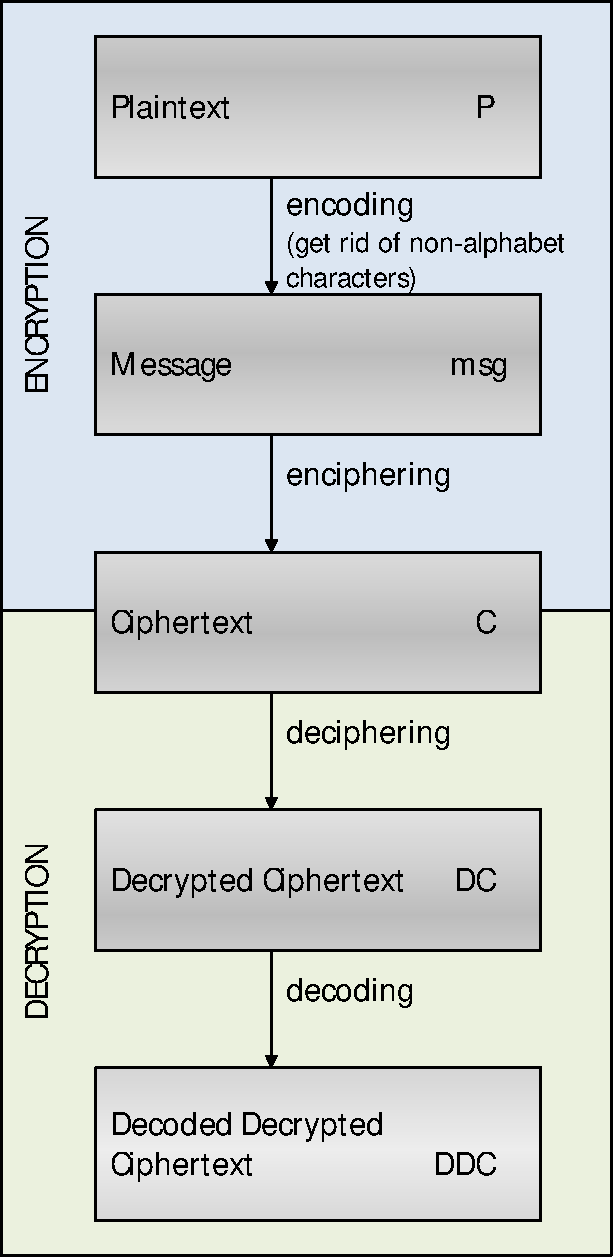
\includegraphics[scale=0.5]{figures/encryption-decryption-en}
\caption{Structure and naming convention of the Sage cipher code examples} 
\label{XXX}
\end{center}
\end{figure}



% ---------------------------------------------------------------------------
\newpage
\subsection{Transposition ciphers}

Transposition ciphers are implemented in the Sage class
\begin{center}
\verb!sage.crypto.classical.TranspositionCryptosystem!
\end{center}
To construct and work with a transposition cipher, we first need to
determine the alphabet that contains the symbols used to build the space of our plaintext
and ciphertext. 
Typically, this alphabet will be the upper-case letters of the
English alphabet, which can be accessed via the function
\begin{center}
\verb!sage.monoids.string_monoid.AlphabeticStrings!
\end{center}
We then need to decide on the block length of a block permutation,
which is the length of the row vector to be used in the simple columns
transposition. This row vector is our key, and it specifies a permutation
of a plaintext.

The following first example of transposition ciphers has block length 14,
and the key is build in a way, that every letter
in the plaintext is shifted to the right by two characters, with wrap
around at the end of the block. That is the encryption process. The decryption process is
shifting each letter of the ciphertext to the left by $14 - 2 = 12$.

\begin{sagecode}
\begin{Verbatim}%
[fontsize=\footnotesize,fontshape=tt]
sage: # transposition cipher using a block length of 14
sage: T = TranspositionCryptosystem(AlphabeticStrings(), 14)
sage: # given plaintext
sage: P   = "a b c d e f g h i j k l m n"
sage: # encryption key
sage: key = [3, 4, 5, 6, 7, 8, 9, 10, 11, 12, 13, 14, 1, 2]
sage:
sage: # encode plaintext (get rid of non-alphabet chars, convert lower-case to upper-case)
sage: msg = T.encoding(P)
sage: # encrypt plaintext by shifting to the left by 2 letters (do it in two steps)
sage: E   = T(key)
sage: C   = E(msg); C
CDEFGHIJKLMNAB
sage:
sage: # decrypt ciphertext by shifting to the left by 12 letters
sage: keyInv = [13, 14, 1, 2, 3, 4, 5, 6, 7, 8, 9, 10, 11, 12]
sage: D   = T(keyInv)
sage: D(C)
ABCDEFGHIJKLMN
sage:
sage: # Representation of key and inverse key as permutations
sage: E
(1,3,5,7,9,11,13)(2,4,6,8,10,12,14)
sage: D
(1,13,11,9,7,5,3)(2,14,12,10,8,6,4)
\end{Verbatim}
\caption{Simple Transposition by shifting (key and inverse key explicitly given)}
\end{sagecode}

\newpage
The second example of transposition ciphers is also a simple shifting column transposition.
But now the code is a little bit more automated: The keys are generated from the shift parameter.

\begin{sagecode}
\begin{Verbatim}%
[fontsize=\footnotesize,fontshape=tt]
sage: # transposition cipher using a block length of 14, code more variable
sage: keylen = 14
sage: shift = 2
sage: A = AlphabeticStrings()
sage: T = TranspositionCryptosystem(A, keylen)
sage:
sage: # construct the plaintext string from the first 14 letters of the alphabet plus blanks
sage: # plaintext   = "A B C D E F G H I J K L M N"
sage: A.gens()
(A, B, C, D, E, F, G, H, I, J, K, L, M, N, O, P, Q, R, S, T, U, V, W, X, Y, Z)
sage: P=''
sage: for i in range(keylen): P=P + " " + str(A.gen(i))
....:
sage: P
' A B C D E F G H I J K L M N'
sage:
sage: # encryption key
sage: # key = [3, 4, 5, 6, 7, 8, 9, 10, 11, 12, 13, 14, 1, 2]
sage: key = [(i+shift).mod(keylen) + 1 for i in range(keylen)]; key
[3, 4, 5, 6, 7, 8, 9, 10, 11, 12, 13, 14, 1, 2]
sage:
sage: # encode plaintext (get rid of non-alphabet chars)
sage: msg = T.encoding(P)
sage: # encrypt plaintext by shifting to the left by 2 letters (do it in one step)
sage: C   = T.enciphering(key, msg); C
CDEFGHIJKLMNAB
sage:
sage: # decrypt ciphertext by shifting to the left by 12 letters
sage: # keyInv = [13, 14, 1, 2, 3, 4, 5, 6, 7, 8, 9, 10, 11, 12]
sage: shiftInv=keylen-shift;
sage: keyInv = [(i+shiftInv).mod(keylen) + 1 for i in range(keylen)]; keyInv
[13, 14, 1, 2, 3, 4, 5, 6, 7, 8, 9, 10, 11, 12]
sage: DC   = T.enciphering(keyInv, C); DC
ABCDEFGHIJKLMN
sage:
sage: # decryption using the "deciphering method with key" instead of "enciphering with keyInv" 
sage: # using the deciphering method requires to change the type of the variable key
sage: DC  = T.deciphering(T(key).key(), C); DC
ABCDEFGHIJKLMN
sage:
sage: # representation of key and inverse key as permutations
sage: T(key)
(1,3,5,7,9,11,13)(2,4,6,8,10,12,14)
sage: T(key).key()
(1,3,5,7,9,11,13)(2,4,6,8,10,12,14)
sage: T(keyInv)
(1,13,11,9,7,5,3)(2,14,12,10,8,6,4)
\end{Verbatim}
\caption{Simple Transposition by shifting (key and inverse key constructed with "range")}
\end{sagecode}

\newpage
In the third example of transposition ciphers we use an arbitrary permutation as key in the
encryption and decryption processes in order to scramble the characters within each
block (block length = number of columns in a simple column transposition).
If the block length is $n$, then the key must be a permutation on $n$ symbols.
The following example uses the method \verb!random_key()! of the class
\verb!TranspositionCryptosystem!. Each call to \verb!random_key()! produces a
different key. Note that therefore your results (key and ciphertext) may be different
from the following example.

\begin{sagecode}
\begin{Verbatim}%
[fontsize=\footnotesize,fontshape=tt]
sage: # Remark: Enciphering here requires, that the length of msg is a multiple of keylen
sage: keylen = 14   # length of key
sage: A = AlphabeticStrings()
sage: T = TranspositionCryptosystem(A, keylen); T
Transposition cryptosystem on Free alphabetic string monoid on A-Z of block length 14
sage:
sage: P = "a b c d e f g h i j k l m n o p q r s t u v w x y z a b"
sage: key = T.random_key(); key
(1,2,3,13,6,5,4,12,7)(11,14)
sage: msg = T.encoding(P); msg
ABCDEFGHIJKLMNOPQRSTUVWXYZAB
sage: C   = T.enciphering(key, msg); C
BCMLDEAHIJNGFKPQAZRSOVWXBUTY
sage: # decryption using the "deciphering method with key" instead of "enciphering with keyInv" 
ssage: DC  = T.deciphering(key, C); DC
ABCDEFGHIJKLMNOPQRSTUVWXYZAB
sage:
sage: # Just another way of decryption: Using "enciphering" with the inverse key
sage: keyInv = T.inverse_key(key); keyInv
(1,7,12,4,5,6,13,3,2)(11,14)
sage: DC     = T.enciphering(keyInv, C); DC
ABCDEFGHIJKLMNOPQRSTUVWXYZAB
sage:
sage: # Test correctness of decryption
sage: msg == DC
True
\end{Verbatim}
\caption{Simple Column Transposition with randomly generated (permutation) key}
\end{sagecode}


\newpage
The fourth example of transposition ciphers additionally shows the key space of a simple
column transposition.

\begin{sagecode}
\begin{Verbatim}%
[fontsize=\footnotesize,fontshape=tt]
sage: keylen = 14   # length of key
sage: A = AlphabeticStrings()
sage: T = TranspositionCryptosystem(A, keylen); T
Transposition cryptosystem on Free alphabetic string monoid on A-Z of block length 14
sage: T.key_space()
Symmetric group of order 14! as a permutation group
sage: # Remark: The key space is not quite correct as also permutations shorter than keylen are counted.
sage:
sage: P = "a b c d e f g h i j k l m n o p q r s t u v w x y z a b"
sage: key = T.random_key(); key
(1,2,7)(3,9)(4,5,10,12,8,13,11)(6,14)
sage: msg = T.encoding(P); msg
ABCDEFGHIJKLMNOPQRSTUVWXYZAB
sage:
sage: # enciphering in one and in two steps
sage: C   = T.enciphering(key, msg); C
BGIEJNAMCLDHKFPUWSXBOAQZRVYT
sage:
sage: enc = T(key); enc.key()
(1,2,7)(3,9)(4,5,10,12,8,13,11)(6,14)
sage: C = enc(msg); C
BGIEJNAMCLDHKFPUWSXBOAQZRVYT
sage:
sage: # deciphering
sage: DC  = T.deciphering(key, C); DC
ABCDEFGHIJKLMNOPQRSTUVWXYZAB
\end{Verbatim}
\caption{Simple Column Transposition (showing the key\_space)}
\end{sagecode}



% ---------------------------------------------------------------------------
\newpage
\subsection{Substitution ciphers}

Substitution cryptosystems are implemented in Sage in the class
\begin{center}
\verb!sage.crypto.classical.SubstitutionCryptosystem!
\end{center}

\noindent The following code sample uses Sage to construct a substitution
cipher with a random key. A random key can be generated using the
method \verb!random_key()! of the class
\texttt{SubstitutionCryp\-to\-system}. Different keys determine different
substitution ciphers. So each call to \verb!random_key()! returns
different results.

\begin{sagecode}
\begin{Verbatim}%
[fontsize=\footnotesize,fontshape=tt]
sage: # plaintext/ciphertext alphabet
sage: A   = AlphabeticStrings()
sage: S   = SubstitutionCryptosystem(A)
sage:
sage: P   = "Substitute this with something else better."
sage: key = S.random_key(); key
INZDHFUXJPATQOYLKSWGVECMRB
sage:
sage: # method encoding can be called from A or from T
sage: msg = A.encoding(P); msg
SUBSTITUTETHISWITHSOMETHINGELSEBETTER
sage: C   = S.enciphering(key, msg); C
WVNWGJGVGHGXJWCJGXWYQHGXJOUHTWHNHGGHS
sage:
sage: #### We now decrypt the ciphertext to recover our plaintext.
sage:
sage: DC  = S.deciphering(key, C); DC
SUBSTITUTETHISWITHSOMETHINGELSEBETTER
sage: msg == DC
True
\end{Verbatim}
\caption{Monoalphabetic Substitution with randomly generated key}
\end{sagecode}



% ---------------------------------------------------------------------------
\newpage
\subsection{Caesar cipher}

The following example uses Sage to construct a Caesar
cipher.

\begin{sagecode}
\begin{Verbatim}%
[fontsize=\footnotesize,fontshape=tt]
sage: # plaintext/ciphertext alphabet
sage: A = AlphabeticStrings()
sage: P = "Shift the alphabet three positions to the right."
sage:
sage: # construct Caesar cipher
sage: S = SubstitutionCryptosystem(A)
sage: key = A([3, 4, 5, 6, 7, 8, 9, 10, 11, 12, 13, 14, 15, 16, 17, 18, 19, \
....:          20, 21, 22, 23, 24, 25, 0, 1, 2])
sage:
sage: # encrypt message
sage: msg     = A.encoding(P); msg
SHIFTTHEALPHABETTHREEPOSITIONSTOTHERIGHT
sage: encrypt = S(key); encrypt
DEFGHIJKLMNOPQRSTUVWXYZABC
sage: C       = encrypt(msg); C
VKLIWWKHDOSKDEHWWKUHHSRVLWLRQVWRWKHULJKW
sage:
sage: #### Next, we recover the plaintext.
sage:
sage: # decrypt message
sage: keyInv = A([23, 24, 25, 0, 1, 2, 3, 4, 5, 6, 7, 8, 9, 10, 11, 12, 13, \
....:             14, 15, 16, 17, 18, 19, 20, 21, 22])
sage: decrypt = S(keyInv); decrypt
XYZABCDEFGHIJKLMNOPQRSTUVW
sage: DC      = decrypt(C); DC
SHIFTTHEALPHABETTHREEPOSITIONSTOTHERIGHT
sage: msg == DC
True
\end{Verbatim}
\caption{Caesar (substitution by shifting the alphabet; key explicitly given, step-by-step approach)}
\end{sagecode}


\newpage
\noindent The second Caesar sample does the same, but the code is more sophisticated/automated/var\-i\-a\-ble.

\begin{sagecode}
\begin{Verbatim}%
[fontsize=\footnotesize,fontshape=tt]
sage: # plaintext/ciphertext alphabet
sage: A = AlphabeticStrings()
sage: keylen = len(A.gens()); keylen
26
sage: shift  = 3
sage: P = "Shift the alphabet three positions to the right."
sage:
sage: # construct Caesar cipher
sage: S = SubstitutionCryptosystem(A)
sage: S
Substitution cryptosystem on Free alphabetic string monoid on A-Z
sage: # key = A([3, 4, 5, 6, 7, 8, 9, 10, 11, 12, 13, 14, 15, 16, 17, 18, 19, \
sage: #          20, 21, 22, 23, 24, 25, 0, 1, 2])
sage: key = [(i+shift).mod(keylen) for i in range(keylen)];
sage: key = A(key); key
DEFGHIJKLMNOPQRSTUVWXYZABC
sage: len(key)
26
sage:
sage: # encrypt message
sage: msg     = A.encoding(P); msg
SHIFTTHEALPHABETTHREEPOSITIONSTOTHERIGHT
sage: C       = S.enciphering(key, msg); C
VKLIWWKHDOSKDEHWWKUHHSRVLWLRQVWRWKHULJKW
sage:
sage: #### Next, we recover the plaintext.
sage:
sage: # decrypt message
sage: # keyInv = A([23, 24, 25, 0, 1, 2, 3, 4, 5, 6, 7, 8, 9, 10, 11, 12, 13, \
sage: #             14, 15, 16, 17, 18, 19, 20, 21, 22])
sage: shiftInv=keylen-shift;
sage: keyInv = [(i+shiftInv).mod(keylen) for i in range(keylen)];
sage: keyInv = A(keyInv); keyInv
XYZABCDEFGHIJKLMNOPQRSTUVW
sage: DC     = S.enciphering(keyInv, C); DC
SHIFTTHEALPHABETTHREEPOSITIONSTOTHERIGHT
sage:
sage: # Just another way of decryption: Using "deciphering" with the key
sage: DC     = S.deciphering(key, C); DC
SHIFTTHEALPHABETTHREEPOSITIONSTOTHERIGHT
sage:
sage: msg == DC
True
\end{Verbatim}
\caption{Caesar (substitution by shifting the alphabet; substitution keys are generated)}
\end{sagecode}



% ---------------------------------------------------------------------------
\newpage
\subsection{Substitution with symbols}

In the following Sage example the symbols are from the binary number
system. A monoalphabetic substitution cipher with a binary alphabet has very little
security: Because the plaintext/ciphertext alphabet has only the two elements
0 and 1, there are only two keys possible: (0 1) and (1 0). Remark: In each key of a
substitution cipher all symbols of the alphabet have to appear once.

\begin{sagecode}
\begin{Verbatim}%
[fontsize=\footnotesize,fontshape=tt]
sage: # the plaintext/ciphertext alphabet
sage: A = BinaryStrings()
sage: # substitution cipher over the alphabet A; no keylen argument possible
sage: S = SubstitutionCryptosystem(A); S
Substitution cryptosystem on Free binary string monoid
sage: # to have a substitute for each symbol, key has always the length of the alphabet
sage: key = S.random_key(); key
10
sage: len(key)
2
sage: P = "Working with binary numbers."
sage: # encryption
sage: msg = A.encoding(P); msg
01010111011011110111001001101011011010010110111001100111001000000111011101101\
00101110100011010000010000001100010011010010110111001100001011100100111100100\
1000000110111001110101011011010110001001100101011100100111001100101110
sage: C   = S.enciphering(key, msg); C
10101000100100001000110110010100100101101001000110011000110111111000100010010\
11010001011100101111101111110011101100101101001000110011110100011011000011011\
0111111001000110001010100100101001110110011010100011011000110011010001
sage: # decryption
sage: DC  = S.deciphering(key, C); DC
01010111011011110111001001101011011010010110111001100111001000000111011101101\
00101110100011010000010000001100010011010010110111001100001011100100111100100\
1000000110111001110101011011010110001001100101011100100111001100101110
sage: msg == DC
True
\end{Verbatim}
\caption{Monoalphabetic substitution with a binary alphabet}
\end{sagecode}



\newpage
The second sample of a monoalphabetic substitution with symbols uses  a larger alphabet
as plaintext/ciphertext space as the first sample. Here the hexadecimal number system
is used as substitution alphabet.

\begin{sagecode}
\begin{Verbatim}%
[fontsize=\footnotesize,fontshape=tt]
sage: A = HexadecimalStrings()
sage: S = SubstitutionCryptosystem(A)
sage: key = S.random_key(); key
2b56a4e701c98df3
sage: len(key)
16
sage: # Number of possible keys
sage: factorial(len(key))
20922789888000
sage: P   = "Working with a larger alphabet."
sage:
sage: msg = A.encoding(P); msg
576f726b696e6720776974682061206c617267657220616c7068616265742e
sage: C   = S.enciphering(key, msg); C
47e375e9e1efe75277e17ae052eb52e8eb75e7e47552ebe872e0ebe5e47a5f
sage: DC  = S.deciphering(key, C); DC
576f726b696e6720776974682061206c617267657220616c7068616265742e
sage: msg == DC
True
sage:
sage: # Conversion hex back to ASCII:
sage: # - AlphabeticStrings() and HexadecimalStrings() don't have according methods.
sage: # - So we used Python:
sage: #   - repr(DC) converts the StringMonoidElement DC to a string
sage: #     still containing hex symbols;
sage: #   - binascii.a2b_hex converts this hex string to an ASCII string.
sage: import binascii
sage: DDC = binascii.a2b_hex(repr(DC)); DDC
'Working with a larger alphabet.'
sage:
sage: P == DDC
True
\end{Verbatim}
\caption{Monoalphabetic substitution with a hexadecimal alphabet (and decoding in Py\-thon)}
\end{sagecode}



% ---------------------------------------------------------------------------
\newpage
\subsection{Vigen{\`e}re cipher}

The Vigen{\`e}re cipher is implemented in the Sage class
\begin{center}
\verb!sage.crypto.classical.VigenereCryptosystem!
\end{center}

\noindent For our ciphertext/plaintext space, we can work with the upper-case
letters of the English alphabet, the binary number system, the
octal number system, or the hexadecimal number system. Here is an
example using the class \verb!AlphabeticStrings!, which implements
the English capital letters.

\begin{sagecode}
\begin{Verbatim}%
[fontsize=\footnotesize,fontshape=tt]
sage: # construct Vigenere cipher
sage: keylen = 14
sage: A = AlphabeticStrings()
sage: V = VigenereCryptosystem(A, keylen); V
Vigenere cryptosystem on Free alphabetic string monoid on A-Z of period 14
sage:
sage: # alternative: given key: key = A('ABCDEFGHIJKLMN'); key
sage: key = V.random_key(); key
WSSSEEGVVAARUD
sage: len(key)
14
sage:
sage: # encoding
sage: P = "The Vigenere cipher is polyalphabetic."
sage: len(P)
38
sage: msg = V.encoding(P); msg     # alternative: msg = A.encoding(P); msg
THEVIGENERECIPHERISPOLYALPHABETIC
sage:
sage: # encryption [2 alternative ways (in two steps or in one): both work]
sage: # encrypt = V(key); encrypt
sage: # C = encrypt(msg); C
sage: C   = V.enciphering(key, msg); C
PZWNMKKIZRETCSDWJAWTUGTALGBDXWLAG
sage:
sage: # decryption
sage: DC  = V.deciphering(key, C); DC
THEVIGENERECIPHERISPOLYALPHABETIC
sage: msg == DC
True
\end{Verbatim}
\caption{Vigen{\`e}re cipher}
\end{sagecode}




% ---------------------------------------------------------------------------
\newpage
\subsection{Hill cipher}

The Hill~\cite{pp:Hill1929,pp:Hill1931} or matrix cipher is more
mathematically sophisticated than other ciphers mentioned in this
chapter. The encryption/decryption key of this cipher is an invertible
square matrix, and the plaintext/ciphertext is processed also as a matrix.
The encryption and decryption processes use matrix operations. The Hill
cipher is implemented in the Sage class
\begin{center}
\verb!sage.crypto.classical.HillCryptosystem!
\end{center}

In the following example our plaintext/ciphertext space is the
capital letters of the English alphabet. In the Hill cipher, each
letter of this alphabet is assigned a unique integer modulo 26.

\begin{sagecode}
\begin{Verbatim}%
[fontsize=\footnotesize,fontshape=tt]
sage: # construct a Hill cipher
sage: keylen = 19    # keylen = 3  # Alternative key length with non-random small key
sage: A = AlphabeticStrings()
sage: H = HillCryptosystem(A, keylen); H
Hill cryptosystem on Free alphabetic string monoid on A-Z of block length 19
sage:
sage: # To create key non-randomly, HKS is necessary [even H.key_space() is not enough].
sage: # HKS = H.key_space()
sage: # key = HKS([[1,0,1],[0,1,1],[2,2,3]]); key
sage:
sage: # Random key creation
sage: key = H.random_key(); key
[10  7  5  2  0  6 10 23 15  7 17 19 18  2  9 12  0 10 11]
[23  1  1 10  4  9 21  1 25 22 19  8 17 22 15  8 12 25 22]
[ 4 12 16 15  1 12 24  5  9 13  5 15  8 21 23 24 22 20  6]
[ 5 11  6  7  3 12  8  9 21 20  9  4 16 18 10  3  2 23 18]
[ 8 22 14 14 20 13 21 19  3 13  2 11 13 23  9 25 25  6  8]
[24 25  8 24  7 18  3 20  6 11 25  5  6 19  7 24  2  4 10]
[15 25 11  1  4  7 11 24 20  2 18  4  9  8 12 19 24  0 12]
[14  6  2  9 11 20 13  4 10 11  4 23 14 22 14 16  9 12 18]
[12 10 21  5 21 15 16 17 19 20  1  1 15  5  0  2 23  4 14]
[21 15 15 16 15 20  4 10 25  7 15  4  7 12 24  9 19 10  6]
[25 15  2  3 17 23 21 16  8 18 23  4 22 11 15 19  6  0 15]
[14 23  9  3 18 15 10 18  7  5 12 23 11  9 22 21 20  4 14]
[ 3  6  8 13 20 16 11  1 13 10  4 21 25 15 12  3  0 11 18]
[21 25 14  6 11  3 21  0 19 17  5  8  5  4  9  2 23 19 15]
[ 8 11  9 11 20 15  6  1  3 18 18 22 16 17  6  3 15 11  2]
[21 15  5 22  2  9  0  4 22 10  2 10 19 19 17 19  1 21  4]
[ 7 17  9  2 15  5 14  3  6  9 12 12 22 15  8  4 21 14 19]
[19 14 24 19  7  5 22 22 13 14  7 18 17 19 25  2  1 23  6]
[ 2  6 14 22 17  7 23  6 22  7 13 20  0 14 23 17  6  1 12]
sage:
sage: # encoding and encryption
sage: P = "Hill or matrix cipher uses matrix operations."
sage: len(P)
45
sage: # implementation requires: Length of msg is a multiple of matrix dimension (block_length)
sage: msg = H.encoding(P); msg
HILLORMATRIXCIPHERUSESMATRIXOPERATIONS
sage: len(msg)
38
sage:
sage: # encryption
sage: C  = H.enciphering(key, msg); C
CRWCKPRVYXNBRZTNZCTQWFWSDWBCHABGMNEHVP
sage:
sage: # decryption
sage: DC  = H.deciphering(key, C); DC
HILLORMATRIXCIPHERUSESMATRIXOPERATIONS
sage: msg == DC
True
sage:
sage: # alternative decryption using inverse matrix
sage: keyInv = H.inverse_key(key); keyInv
[ 6 23  1 23  3 12 17 22  6 16 22 14 18  3  1 10 21 16 20]
[18 23 15 25 24 23  7  4 10  7 21  7  9  0 13 22  5  5 23]
...
[10 11 12  6 11 17 13  9 19 16 14 24  4  8  5 16 18 20  1]
[19 16 16 21  1 19  7 12  3 18  1 17  7 10 24 21  7 16 11]
sage: DC     = H.enciphering(keyInv, C); DC
HILLORMATRIXCIPHERUSESMATRIXOPERATIONS
\end{Verbatim}
\caption{Hill cipher}
\end{sagecode}







% --------------------------------------------------------------------------
\newpage
\begin{thebibliography}{99999}
\addcontentsline{toc}{section}{Bibliography}

\bibitem[ACA2002]{pp:ACA2002} \index{ACA 2002}
   American Cryptogram Association, \\
   {\em Length and Standards for all ACA Ciphers}, \\
   2002.\\
   \href{http://www.cryptogram.org/cdb/aca.info/aca.and.you/chap08.html#}
   {\texttt{http://www.cryptogram.org/cdb/aca.info/aca.and.you/chap08.html\#}}

\bibitem[Bauer1995]{pp:Bauer1995} \index{Bauer 1995}
    Friedrich L. Bauer, \\
    {\em Entzifferte Geheimnisse}, Springer, 1995.

\bibitem[Bauer2000]{pp:Bauer2000} \index{Bauer 2000}
    Friedrich L. Bauer, \\
    {\em Decrypted Secrets}, Springer 1997, 2nd edition 2000.
	
\bibitem[Crowley2000]{pp:Crowley2000} \index{Crowley 2000}
   Paul Crowley, \\
   {\em Mirdek: A card cipher inspired by ``Solitaire''}, \\
   2000.\\
   \href{http://www.ciphergoth.org/crypto/mirdek/}
   {\texttt{http://www.ciphergoth.org/crypto/mirdek/}}

\bibitem[DA1999]{pp:DA1999} \index{DA 1999}
   Data encryption page of the ThinkQuest Team 27158 for ThinkQuest 1999 \\
   (no update since 1999, no search possibility), \\
   1999.\\
   \href{http://library.thinkquest.org/27158/}
   {\texttt{http://library.thinkquest.org/27158/}}

\bibitem[Goebel2003]{pp:Goebel2003} \index{Goebel 2003}
   Greg Goebel, \\
   {\em Codes, Ciphers and Codebreaking}, \\
   2003.\\
   \href{http://www.vectorsite.net/ttcode.htm}
   {\texttt{http://www.vectorsite.net/ttcode.htm}}

\bibitem[Hill1929]{pp:Hill1929} \index{Hill 1929}
   Lester S. Hill,\\
   ``Cryptography in an Algebraic Alphabet,''
   \emph{The American Mathematical Monthly}, 36(6):306--312, 1929.

\bibitem[Hill1931]{pp:Hill1931} \index{Hill 1931}
   Lester S. Hill,\\
   ``Concerning Certain Linear Transformation Apparatus of Cryptography,''
   \emph{The American Mathematical Monthly}, 38(3):135--154, 1931.

\bibitem[Nichols1996]{pp:Nichols1996} \index{Nichols 1996} 
    Randall K. Nichols, \\
    {\em Classical Cryptography Course, Volume 1 and 2}, \\
    Aegean Park Press 1996;
    or in 12 lessons online at \\
    \href{http://www.fortunecity.com/skyscraper/coding/379/lesson1.htm}
    {\texttt{http://www.fortunecity.com/skyscraper/coding/379/lesson1.htm}}

\bibitem[Savard1999]{pp:Savard1999} \index{Savard 1999}
	John J. G. Savard, \\
	{\em A Cryptographic Compendium}, \\
	1999.\\
	\href{http://www.hypermaths.org/quadibloc/crypto/jscrypt.htm}
	{\texttt{http://www.hypermaths.org/quadibloc/crypto/jscrypt.htm}}
	
\bibitem[Schmeh2004]{pp:Schmeh2004}  \index{Schmeh 2004}
        Klaus Schmeh, \\
        {\em Die Welt der geheimen Zeichen. Die faszinierende Geschichte
        der Verschl\"usselung},\\ 
        W3L Verlag Bochum, 1. Auflage 2004.

\bibitem[Schmeh2007]{pp:Schmeh2007}  \index{Schmeh 2007}
        Klaus Schmeh, \\
        {\em Codeknacker gegen Codemacher. Die faszinierende Geschichte der Verschl\"usselung.},\\ 
        W3L Verlag Bochum, 2. Auflage 2007.\\
	This is most current among the books dealing in a comprehensive manner
	with the history of cryptology. It contains a small collection of solved
	and unsolved crypto riddles. One of the challenges deals with a double
	column transposition using two long keys, which are differently in addition.

\bibitem[Schneier1999]{pp:Schneier1999}
	Bruce Schneier, \\
	{\em The Solitaire Encryption Algorithm}, \\
	version 1.2, 1999.\\
	\href{http://www.schneier.com/solitaire.html}
	{\texttt{http://www.schneier.com/solitaire.html}}

\bibitem[Singh2001]{pp:Singh2001} \index{Singh 2001}
	Simon Singh, \\
	{\em Geheime Botschaften. Die Kunst der Verschl\"usselung von der 
        Antike bis in die Zeiten des Internet}, \\
	dtv, 2001.

\bibitem[ThinkQuest1999]{pp:ThinkQuest1999} \index{ThinkQuest 1999}
	ThinkQuest Team 27158, \\
	{\em Data Encryption}, \\
	1999.\\
	\href{http://library.thinkquest.org/27158/}
	{\texttt{http://library.thinkquest.org/27158/} }

\end{thebibliography}









% Local Variables:
% TeX-master: "../script-en.tex"
% End:


\renewcommand{\CTBChapName}{(Chap Primes)}        % $Id$
%%%%%%%%%%%%%%%%%%%%%%%%%%%%%%%%%%%%%%%%%%%%%%%%%%%%%%%%%%%%%%%%%%%%%%%%%%
%
% C H A P T E R   T H R E E :  P R I M E S
%
%%%%%%%%%%%%%%%%%%%%%%%%%%%%%%%%%%%%%%%%%%%%%%%%%%%%%%%%%%%%%%%%%%%%%%%%%%

\newpage
\hypertarget{Kapitel_2}{}
\section{Prime Numbers}
\label{Label_Kapitel_2}
(Bernhard Esslinger, May 1999; Updates Nov. 2000, Dec. 2001, June 2003, May 2005, March 2006, May 2007)

\begin{center}
\fbox{\parbox{15cm}{
    \emph{Albert Einstein\footnotemark:}\\
    Progress requires exchange of knowledge.
}}
\end{center}
\addtocounter{footnote}{0}\footnotetext{%
  Albert Einstein, German physicist and Nobel Prize winner, 
  Mar 14, 1879 $-$ Apr 14, 1955.
}

% --------------------------------------------------------------------------
\subsection{What are prime numbers?}
\index{Prime number} \index{Number!prime}
Prime numbers are whole, positive numbers greater than or equal to $2$ that can
only be divided by 1 and themselves. All other natural numbers greater than or
equal to $2$ can be formed by multiplying prime numbers.

The {\em natural} \index{Number!natural} numbers $\mathbb{N}=\{1, 2, 3, 4,\cdots \}$ thus comprise 
\begin{itemize}
   \item the number $1$ (the unit value)
   \item the primes and
   \item the composite numbers.
\end{itemize}

Prime numbers are particularly important for 3 reasons:
\begin{itemize}
  \item In number theory, they are considered to be the basic components of
natural numbers, upon which numerous brilliant mathematical ideas are based.
  \item They are of extreme practical importance in modern
\index{Cryptography!modern} cryptography (public key \index{Cryptography!public key} cryptography). The most common public key procedure, invented at the end of
the 1970's, is \index{RSA} RSA encryption. Only using (large) prime numbers for
particular parameters can you guarantee that an algorithm is secure, both for
the RSA procedure and for even more modern procedures (digital
\index{Signature!digital} signature, elliptic curves).
  \item The search for the largest known prime numbers does not have any
practical usage known to date, but requires the best computers, is an excellent
benchmark (possibility for determining the performance\index{Performance} of computers) and leads
to new calculation methods on many computers \\ (see also:
\href{http://www.mersenne.org/prime.htm}{\tt
http://www.mersenne.org/prime.htm}).
\end{itemize}
Many people have been fascinated by prime numbers over the past two millennia.
Ambition to make new discoveries about prime numbers has often resulted in
brilliant ideas and conclusions. The following section provides an easily
comprehensible introduction to the basics of prime numbers. We will also explain
what is known about the distribution (density, number of prime numbers in
particular intervals) of prime numbers and how prime number tests work.


% --------------------------------------------------------------------------
\subsection{Prime numbers in mathematics}\label{primesinmath}

Every whole number has a factor. The number 1 only has one factor,
itself, whereas the number $12$ has the six factors $1, 2, 3, 4,
6, 12$. Many numbers can only be divided by themselves and by $1$.
With respect to multiplication, these are the ``atoms'' in the
area of numbers. Such numbers are called prime numbers.

In mathematics, a slightly different (but equivalent) definition is used.

\begin{definition}\label{def-pz-prime}
A whole number $p \in {\bf N}$ is called prime \index{Number!prime} if
$p > 1$ and $p$ only possesses the trivial factors $\pm 1$ and $\pm p$.
\end{definition}


By definition, the number $1$ is not a prime number. In the following sections,
$p$ will always denote a prime number.

The sequence of prime numbers starts with $$ 2,~ 3,~ 5,~ 7, ~ 11, ~ 13, ~
17, ~ 19, ~ 23, ~ 29, ~ 31, ~ 37, ~ 41, ~ 43, ~ 47, ~ 53, ~ 59, ~ 61,
~ 67, ~ 71, ~ 73, ~ 79, ~ 83, ~ 89, ~ 97, \cdots . $$
The first 100 numbers include precisely 25 prime numbers. After this,
the percentage of primes constantly decreases. Prime numbers can be
factorised in a uniquely {\em trivial} way: 
$$5 = 1 \cdot 5,\quad  17 = 1 \cdot 17, \quad 1,013 = 1 \cdot 1,013,  \quad
1,296,409 = 1 \cdot 1,296,409.$$
All numbers that have $2$ or more factors not equal 1 are called 
\index{Number!composite} {\em composite} numbers. 
These include $$ 4 = 2 \cdot 2, \quad 6 = 2\cdot 3 $$ as well
as numbers that {\em look like primes}, but are in fact composite:
$$ 91 = 7 \cdot 13, \quad 161=7 \cdot 23, \quad 767 =13 \cdot 59. $$

\begin{theorem}\label{thm-pz-sqr}
Each whole number $m$ greater than $1$ possesses a lowest factor greater than
$1$. This is a prime number $p$. Unless $m$ is a prime number itself, then: $p$
is less than or equal to the square root of $m$.
\end{theorem}

All whole numbers greater than $1$ can be expressed as a product of prime
numbers --- in a unique way. This is the claim of the 1st fundamental theorem of
number theory (= fundamental theorem of arithmetic = fundamental building block
of all positive integers).\index{Number theory!fundamental theorem}

\begin{theorem}\label{thm-pz-prod}
Each element $n$ of the natural numbers greater than $1$ can be written as the
product $n = p_1 \cdot p_2 \dots p_m$ of prime numbers. If two such
factorisations $$n =  p_1 \cdot p_2 \cdot \cdots \cdot p_m = p'_1 \cdot p'_2 \cdots
p'_{m'}$$ are given, then they can be reordered such that $\;m = m'\;$ and for
all $i$:  $\;p_i = p'_i$. \\
($p_1, p_2, \dots, p_m$ are called the prime factors of n).
\end{theorem}

In other words: each natural number other than $1$ can be written as a product
of prime numbers in precisely one way, if we ignore the order of the factors.
The factors are therefore unique (the {\em expression as a product of factors}
is unique)! For example, $$ 60 = 2 \cdot 2 \cdot 3 \cdot 5 = 2^2\cdot 3^1 \cdot
5^1. $$
And this --- other than changing the order of the factors --- is the only way in
which the number $60$ can be factorised. If you allow numbers other than primes
as factors, there are several ways of factorising integers and the uniqueness \hypertarget{uniqueness}{} is
lost: $$ 60 = 1 \cdot 60 = 2 \cdot 30 = 4 \cdot 15 = 5 \cdot 12 =6 \cdot 10 = 2
\cdot 3 \cdot 10 = 2 \cdot 5 \cdot 6 = 3 \cdot 4 \cdot 5 = \cdots . $$

The following section is aimed more at those familiar with mathematical logic:
The 1st fundamental theorem only appears to be obvious \label{remFundTheoOfArithm}. We can construct
numerous other sets of numbers (i.e. other than positive whole numbers greater
than 1), for which numbers in the set cannot be expressed uniquely as a product
of the prime numbers of the set: In the set $M = \{1, 5, 10, 15, 20, \cdots\}$
there is no equivalent to the fundamental theorem under multiplication. The
first five prime numbers of this sequence are $5, 10, 15, 20, 30$ (note: $10$ is
prime, because $5$ is not a factor of $10$ in this set --- the result is not an
element of the given basic set $M$). Because the following applies in $M$: $$
100 = 5 \cdot 20 = 10 \cdot 10 $$ and $5, 10, 20$ are all prime numbers in this
set, the expression as a product of prime factors is not unique here.

% --------------------------------------------------------------------------
\subsection{How many prime numbers are there?}

For the natural numbers, the primes can be compared to elements in chemistry or
the elementary particles in physics (see \cite[p. 22]{Blum1999}).

Although there are only $92$ natural chemical elements, the number of prime
numbers is unlimited. Even the Greek, \index{Euclid} Euclid%
\footnote{Euclid,
a Greek mathematician of 4th and 3rd century B.C. He worked at the
Egyptian academy of Alexandria and wrote ``The Elements'', the most well 
known systematically textbook of the Greek mathematics.} 
knew this in the third century B.C.
\begin{theorem}[Euclid\footnote{The common usage of the term does not denote Euclid as the inventor of the theorem rather;
the true inventor is merely not as prominent. The theorem has already been distinguished
and proven in Euclid's Elements (Book IX, theorem 20). The phraseology is remarkable due to 
the fact that the word infinite is not used. The text reads as followed
$$
O\acute{\iota}~\pi\varrho\tilde{\omega}\tau o \iota~\grave{\alpha}\varrho\iota\vartheta\mu o\grave{\iota}~
\pi\lambda\varepsilon\acute{\iota}o \upsilon\varsigma~\varepsilon\grave{\iota}\sigma\grave{\iota}~
\pi\alpha\nu\tau\grave{o}\varsigma~\tau o \tilde{\upsilon}~
\pi\varrho o \tau\varepsilon\vartheta\acute{\varepsilon}\nu\tau o \varsigma~
\pi\lambda\acute{\eta}\vartheta\ o \upsilon\varsigma~
\pi\varrho\acute{\omega}\tau\omega\nu~
\grave{\alpha}\varrho\iota\vartheta\mu\tilde{\omega}\nu,
$$
the English translation of which is: the prime numbers are more than 
any previously existing amount of prime numbers.
}]\label{thm-pz-euklid} % Ende der Fu�note
% Fussnote VOR "]" in [Euclid], damit kein Leerraum vor der Fussnotennummer.
% Vorher stand da: ...(Euclid). BLANK Fussnote und das Blank stoerte.
% Nun steht die Fussnote direkt hinter "Euclid" und vor der ")".
% Eigentlich h�tte ich sie gerne direkt hinter "(Euclid)", noch vor dem 
% automatisch gesetzten Punkt. 
The sequence of prime numbers does not discontinue.
Therefore, the quantity of prime numbers is infinite.
\end{theorem}
His proof that there is an infinite number of
primes is still considered to be a brilliant mathematical consideration and
conclusion today (proof by contradiction \index{Proof by contradiction}). 
He assumed that there is only a finite number of primes and therefore a 
largest prime number. Based on this assumption, he drew logical conclusions
until he obtained an obvious contradiction. This meant that something must
be wrong. As there were no mistakes in the chain of conclusions, it could
only be the assumption that was wrong. Therefore, there must be an infinite
number of primes!

\hypertarget{euclid}{}
\paragraph{Euclid's proof by contradiction}
\index{Euclid's proof by contradiction}\index{Proof by contradiction}
goes as follows:

\begin{Proof}{}
{\bf Assumption:} \quad There is a {\em finite} number of primes. \\*[4pt] {\bf
Conclusion:} \quad Then these can be listed $p_1 < p_2 < p_3 < \dots < p_n$,
where $n$ is the (finite) number of prime numbers. $p_n$ is therefore the
largest prime. Euclid now looks at the number $a = p_1 \cdot p_2 \cdots p_n +1$.
This number cannot be a prime number because it is not included in our list of
primes. It must therefore be divisible by a prime, i.e. there is a natural
number $i$ between $1$ and $n$, such that $p_i$ divides the number $a$. Of
course, $p_i$ also divides the product $a-1 = p_1 \cdot p_2 \cdots p_n$, because
$p_i$ is a factor of $a-1$. Since $ p_i $ divides the numbers $ a $ and $ a-1 $,
it also divides the difference of these numbers. Thus: $p_i$ divides  $a - (a-1)
= 1$. $p_i$ must therefore divide $1$, which is impossible. \\*[4pt] {\bf
Contradiction:} \quad Our assumption was false.

Thus there is an {\em infinite} number of primes
(Cross-reference: \hyperlink{primhfk}{overview} under \ref{s:primhfk} of 
the number of prime numbers in various intervals).
\end{Proof} 

\par \vskip + 10pt

Here we should perhaps mention yet another fact which is initially somewhat surprising. 
Namely, in the prime numbers sequence $p_1, p_2, \cdots,$ gaps between prime numbers can have
an individually determined length $n$. It is undeniable that under the $n$
succession of natural numbers
$$(n+1)!+2,\cdots, (n+1)!+(n+1),
$$
none of them is a prime number since in order, the numbers $2,3,\cdots,(n+1)$  
are comprised respectively as real divisors. 
($n!$ means the product of the first $n$ natural numbers therefore 
$ n!= n*(n-1)*\cdots *2*1$).


% --------------------------------------------------------------------------
% --------------------------------------------------------------------------
\vskip + 20pt
\subsection{The search for extremely large primes}
\label{search_for_very_big_primes}   % chap. 3.4

The largest prime numbers known today have several millions digits, 
which is too big for us to imagine. The number of elementary particles in
the universe is estimated to be ``only'' a $80$-digit number 
\hyperlink{grosord}{(See: overview under \ref{s:grosord}
of various orders of magnitude / dimensions)}.


% --------------------------------------------------------------------------
\hypertarget{RecordPrimes}{}
\subsubsection{The 20 largest known primes (as of May 2007)}  % Eyecatcher_neue-Mersenne
\label{RecordPrimes}
\index{Prime number!records}

The following table contains the current record primes and
a description of its particular number type\footnote{%
An up-to-date version can be found in the internet at
     \href{http://primes.utm.edu/largest.html}
  {\texttt{http://primes.utm.edu/largest.html}}.
}:

\index{Mersenne!number!generalized}
\index{Fermat!number!generalized} 

\begin{table}[h]
\begin{center}
\begin{tabular}{|c|cccc|}
\hline    % Eyecatcher_neue-Mersenne
	& {\bf Definition} & {\bf Decimal Digits} & {\bf When} & {\bf Description} \\
\hline
	1  & $2^{32,582,657}-1$ & 9,808,358 & 2006 & Mersenne, 44th known \\
	2  & $2^{30,402,457}-1$ & 9,152,052 & 2005 & Mersenne, 43rd known \\
	3  & $2^{25,964,951}-1$ & 7,816,230 & 2005 & Mersenne, 42nd known \\
	4  & $2^{24,036,583}-1$ & 7,235,733 & 2004 & Mersenne, 41st known \\
	5  & $2^{20,996,011}-1$ & 6,320,430 & 2003 & Mersenne, 40th known \\
	6  & $2^{13,466,917}-1$ & 4,053,946 & 2001 & Mersenne, M-39 \\
	7  & $19,249 \cdot 2^{13,018,586}+1$ & 3,918,990 & 2007 & Generalized Mersenne\footnotemark \\
	8  & $27,653 \cdot 2^{9,167,433}+1$ & 2,759,677 & 2005 & Generalized Mersenne \\



	9  & $28,433 \cdot 2^{7,830,457}+1$ & 2,357,207 & 2004 & Generalized Mersenne \\

	10  & $2^{ 6,972,593}-1$ & 2,098,960 & 1999 & Mersenne, M-38 \\
	11  & $5,359 \cdot 2^{5,054,502}+1$ & 1,521,561 & 2003 & Generalized Mersenne \\

	12  & $4,847 \cdot 2^{3,321,063}+1$ & 999,744 & 2005 & Generalized Mersenne \\
	13  & $3 \cdot 2^{3,136,255}-1$ & 944,108 & 2007 & Generalized Mersenne \\

	14  & $2^{ 3,021,377}-1$ &   909,526 & 1998 & Mersenne, M-37 \\
	15  & $2^{ 2,976,221}-1$ &   895,932 & 1997 & Mersenne, M-36 \\

	16  & $222,361 \cdot 2^{2,854,840}+1$ & 859,398 & 2006 & Generalized Mersenne \\

	17 & $1,372,930^{131,072}+1$ &   804,474 & 2003 & Generalized Fermat\footnotemark \\

	18  & $1,361,244^{131,072}+1$ &   803,988 & 2004 & Generalized Fermat \\
	19  & $1,176,694^{131,072}+1$ &   795,695 & 2003 & Generalized Fermat \\

	20  & $342,673 \cdot 2^{2,639,439}-1$ & 794,556 & 2007 & Generalized Mersenne \\

\hline
\end{tabular}
\caption{The 20 largest known primes and its particular number types
         (as of May 2007)}    % Eyecatcher_neue-Mersenne
\label{L_n_Largest_Kown-Primes}
\end{center}
\end{table} 
\footnotetext{\index{Number!Sierpinski}\index{Seventeen or Bust SoB}%
This number was found within the distributed computing project
``Seventeen or Bust'' (SoB) (\href{http://www.seventeenorbust.com}{\texttt{http://www.seventeenorbust.com}})
% {\href{http://www.mersenne.org} {\tt http://www.mersenne.org}}
at March 26, 2007. While the well known \hyperlink{GIMPS-project}{GIMPS project} (chapter~\ref{zahlentyp_mersenne}) searches for bigger and bigger of the infinitely many primes, there is a chance, that the SoB project could have been completed its
task sometime.

The SoB project tries to prove computationally, that the number $k = 78,557$ is
the smallest Sierpinski number (John Selfridge proved in 1962, that $78,557$ is a Sierpinski number).

The famous Polish mathematician Waclaw Sierpinski (1882 to 1969) proved in
1960, that there exist infinitely many odd integers k, which fulfill the
following property: For all Sierpinski numbers k it is true: All numbers $N = k \cdot 2^{n}+1$ are composite for all integers $n>=1$ (Sierpinski's Composite Number Theorem, \href{http://mathworld.wolfram.com/SierpinskisCompositeNumberTheorem.html}{\texttt{http://mathworld.wolfram.com/SierpinskisCompositeNumberTheorem.html}}).

When the project started in 2002 there have been 17 possible candidates $< 78557$ (this is the reason for the project's name ``Seventeen or Bust''). It is sufficient to find one single counter-example, to exclude a candidate k, which means to find a single $n>=1$, where $N = k \cdot 2^{n}+1$ is prime. So it is only a byproduct of this task that this also generates new monster primes.
} 
\footnotetext{%
Generalized Fermat number: $ 1,372,930^{131,072} + 1 = 1,372,930^{(2^{17})}+1 $
\index{Fermat!number!generalized}  } 
%be_2005: Erzwingen, dass die Abb. noch in diesem Kapitel !

The largest known prime is a Mersenne prime, found by the
\hyperlink{GIMPS-project}{GIMPS project}(chapter~\ref{zahlentyp_mersenne}).

Within the largest known primes there are also numbers of the type
\hyperlink{generalizedMersennenumbers}{generalized Mersenne number}
(chapter~\ref{generalized-mersenne-no1})
and 
\hyperlink{generalizedFermatprimes}{generalized Fermat numbers}
(chapter~\ref{generalized-fermat}).


% --------------------------------------------------------------------------
\hypertarget{MersenneNumbers01}{}
\subsubsection{Special number types -- Mersenne numbers and Mersenne primes} 
\label{zahlentyp_mersenne}
\index{Mersenne!number}

Almost all known huge prime numbers are special candidates, called
\index{Mersenne, Marin} {\em Mersenne numbers}\footnote{%
Marin Mersenne, French priest and mathematician, Sep 08, 1588 $-$ Sep 01, 1648.
\index{Mersenne, Marin}
}
of the form $2^p -1,$ where $p$ is
a prime. Not all Mersenne numbers are prime:

$$
\begin{array}{cl}
2^2 - 1 = 3 & \Rightarrow {\rm prime} \\
2^3 - 1 = 7 & \Rightarrow {\rm prime} \\
2^5 - 1 = 31    & \Rightarrow {\rm prime} \\
2^7 - 1 = 127    & \Rightarrow {\rm prime} \\
2^{11} - 1 = 2,047 = 23 \cdot 89    & \Rightarrow  {\rm NOT~prime} !
\end{array}
$$

\index{Number!Mersenne}\index{Mersenne!number}
\index{Mersenne!theorem} 

Even Mersenne knew that not all Mersenne numbers
are prime (see exponent $p = 11$). 
A prime Mersenne number \index{Mersenne!prime number} is called
Mersenne prime number.  \\
However, he is to be thanked for the interesting conclusion that a number 
of the form $2^n-1$ cannot be a prime number if $n$ is a composite number:

\begin{theorem}[Mersenne]\label{thm-pz-mersenne} 
  If $2^n - 1$ is a prime number, then $n$ is also a prime number.
\end{theorem}

\begin{Proof}{}
The theorem of Mersenne can be proved by contradiction%
\index{Proof by contradiction}.  We therefore assume that
there exists a composite natural number $ n $ (with real factorisation)  
$ n=n_1 \cdot n_2 $
, with the property that $ 2^n -1 $ is a prime number.

From \begin{eqnarray*} (x^r-1)((x^r)^{s-1} + (x^r)^{s-2} + \cdots + x^r +1) & =
&  ((x^r)^s + (x^r)^{s-1} + (x^r)^{s-2} + \cdots + x^r) \\ &  & -((x^r)^{s-1} +
(x^r)^{s-2} + \cdots + x^r +1)  \\ & = & (x^r)^s -1 = x^{rs } -1,
\end{eqnarray*} we conclude \[ 2^{n_1 n_2} - 1 = (2^{n_1} -1)((2^{n_1})^{n_2 -1}
+ (2^{n_1})^{n_2 -2} + \cdots + 2^{n_1} + 1). \]
Because $ 2^n - 1 $ is a prime number, one of the above two factors on the
right-hand side must be equal to 1. This is the case if and only if $ n_1 =1 $
or $ n_2 =1$. But this contradicts our assumption. Therefore the assumption is
false. This means that there exists no composite number $ n, $ such that $ 2^n -
1 $ is a prime.
\end{Proof} 

\vskip + 5pt
\hypertarget{Mer-nums-not-always-prim}{}
Unfortunately this theorem only applies in one direction (the inverse 
statement does not apply, no equivalence): that means that there exist 
prime exponent for which the Mersenne number is {\bf not} prime (see the 
above example $2^{11}-1, $ where $11$ is prime, but $2^{11}-1$ not).

Mersenne claimed that $2^{67}-1$ is a prime number. There is also a mathematical
history behind this claim: it first took over 200 years before 
\index{Lucas, Edouard} Edouard Lucas (1842-1891) proved that this number 
is composite.
However, he argued indirectly and did not name any of the factors. Then Frank
Nelson Cole\index{Cole, Frank Nelson}\footnote{%
Frank Nelson Cole, American mathematician, Sep. 20, 1861 $-$ May 26, 1926.}
showed in 1903 which factors make up this composite number: 
$$ 2^{67} -1
=147, 573, 952, 589, 676, 412, 927 = 193, 707, 721 \cdot 761, 838, 257, 287. $$
He admitted to having worked 20 years on the factorisation 
\index{Factorisation} (expression as a product of prime factors)\footnote{%
  Using CrypTool\index{CrypTool} you can factorize numbers in the 
  following way: menu {\bf Indiv. Procedures \textbackslash{} RSA Cryptosystem 
  \textbackslash{} Factorisation of a Number}. \\
  CrypTool can factorize in a reasonable time numbers no longer than 250 bit.
  Numbers bigger than 1024 bits are currently not accepted by CrypTool. \\
  The current factorization records are listed in chapter \ref{NoteFactorisation}.
  \index{Factorisation!factoring records}
}
of this 21-digit decimal number!

Due to the fact that the exponents of the Mersenne numbers
\index{Mersenne!number} do not use all
natural numbers, but only the primes, the {\em experimental space} is limited
considerably. The currently known Mersenne prime numbers 
\index{Mersenne!prime number} have the exponents\footnote{%
The following page from Landon Curt Noll\index{Noll, Landon Curt} contains 
all Mersenne primes including its date of discovery and its value as number 
and as word:
      \href{http://www.isthe.com/chongo/tech/math/prime/mersenne.html}
   {\texttt{http://www.isthe.com/chongo/tech/math/prime/mersenne.html}}. \\
Also see:
      \href{http://www.utm.edu/}
   {\texttt{http://www.utm.edu/}}.
                             } 
$$
\begin{array}{c}
2; ~ 3; ~ 5; ~ 7; ~ 13; ~ 17; ~ 19; ~ 31; ~ 61; ~ 89; ~ 107; ~ 127;
~ 521; ~ 607; ~ 1,279; ~ 2,203; ~ 2,281; ~ 3,217; ~ 4,253;\\
 4,423; ~ 9,689; ~ 9,941, ~ 11,213; ~ 19,937; ~ 21,701; ~ 23,207; ~ 44,497; ~
86,243; ~ 110,503; ~ 132,049; \\
 216,091; ~ 756,839; ~ 859,433; ~ 1,257,787; ~ 1,398,269; ~ 2,976,221;
 ~ 3,021,377; ~ 6,972,593; \\
 ~ 13,466,917;  ~ 20,996,011;  ~ 24,036,583;  ~ 25,964,951;  ~ 30,402,457,  ~ 32.582.657.
% be_2005_UPDATEN_if-new-mersenne-prime-appears          ~ xxx,xxx,xxx.
\end{array}
$$
Thus    % Eyecatcher_neue-Mersenne
$44$            % be_2005_UPDATEN_if-new-mersenne-prime-appears
Mersenne prime numbers are currently known%
\index{Prime number!Mersenne}\index{Mersenne!prime number}. 

The $19$th number with the exponent $4,253$ was the first with at least $1,000$ digits in  decimal system
(the mathematician Samual \index{Yates, Samual} Yates coined the expression {\em
titanic} \index{Prime number!titanic} prime for this; it was discovered by
Hurwitz in 1961); the $27$th number with the exponent $44,497$ was the first
with at least $10,000$ digits in the decimal system (Yates coined the expression
\index{Prime number!gigantic}  {\em gigantic} prime for this. These names are
now long outdated).


\vskip +25 pt
For the first 39            % be_2005_UPDATEN_if-new-mersenne-prime-appears    % Eyecatcher_neue-Mersenne
Mersenne prime numbers we know that this list is complete.
The exponents until the 40th     % be_2005_UPDATEN_if-new-mersenne-prime-appear    % Eyecatcher_neue-Mersennes
Mersenne prime number have not yet been checked completely\footnote{%
The current status of the check can be found at:
      \href{http://www.mersenne.org/status.htm}
   {\texttt{http://www.mersenne.org/status.htm}}.\\
Hints, how the primality of a number can be checked, are in chapter
\ref{primality_tests}, prime number tests\index{Prime number!test}. }.


\vskip +25 pt
\paragraph{M-37 -- January 1998}\index{Mersenne!prime number!M-37}\mbox{}

The 37th Mersenne prime, $$ 2^{3,021,377} - 1 $$
was found in January 1998 and has 909,526
digits in the decimal system, which corresponds to 33 pages in the newspaper!


\vskip +25 pt
\paragraph{M-38 -- June 1999}\index{Mersenne!prime number!M-38}\mbox{}

The 38th Mersenne prime, called M-38, $$ 2^{6,972,593} - 1 $$
was discovered in June 1999 and has $2,098,960$ digits in the decimal system
(that corresponds to around 77 pages in the newspaper).


\vskip +25 pt
\hypertarget{M-39}{}
\paragraph{M-39 -- December 2001}%
\index{Mersenne!prime number!M-39}\mbox{}

The 39th Mersenne prime, called M-39, $$2^{13,466,917}-1,$$ was
published at December 6, 2001 -- more exactly, the verification of this number,
found at November 14, 2001 by the Canadian student Michael Cameron, was
successfully completed. 
This number has about 4 million decimal digits (exactly 4,053,946 digits).
Trying only to print this number 
$$(924947738006701322247758 \cdots 1130073855470256259071)$$
would require around 200 pages in the Financial Times.

Right now (May 2005) all prime exponents smaller than $ 13.466.917 $ have been
tested and double-checked (see home page of the GIMPS project:
{\href{http://www.mersenne.org} {\tt http://www.mersenne.org}}): so we can
be certain, that this is really the 39th Mersenne prime number and that
there are no smaller undiscovered Mersenne primes (it is common usage to use
the notation M-nn not until it is proven, that the nn-th known Mersenne prime
is really the nn-th Mersenne prime).

%\vskip +15 pt
%\paragraph{Mxxxxxxxxxx -- June 2003 -- M-40 ?}%
%\index{Mersenne!prime number!M-40}\mbox{}
%\vskip +10 pt

%This number was discovered as 40th Mersenne prime (and already called M-40,
%despite it has not been proven yet, whether no further Mersenne prime
%numbers between M-39 und Mxxxxxxxxx do indeed exist), $$2^{xx,xxx,xxx}-1,$$
%at June xx, 2003 -- more exactly, the verification of this number,
%found at June 02, 2003 by xxxxxxxxxx, was
%successfully completed. 
%The initiator and project leader George Woltman only announces a found
%Mersenne number, after another double-check confirms that it is prime.
%This number has about xx million decimal digits
%(exactly xx,xxx,xxx digits).




\vskip +25 pt
\paragraph{GIMPS}\index{GIMPS}\mbox{}
\hypertarget{GIMPS-project}{}

The GIMPS project (Great Internet Mersenne Prime Search)\index{GIMPS} was
founded in 1996 by George Woltman\index{Woltman, George} to search for new
largest Mersenne primes 
({\href{http://www.mersenne.org} {\tt http://www.mersenne.org}}).
Further explanations about this number type can be found under
\hyperlink{MersenneNumbers02}{Mersenne numbers} and 
\hyperlink{MersenneNumbers01}{Mersenne primes}.

Right now the GIMPS project has discovered ten
   % be_2005_UPDATEN_if-new-mersenne-prime-appears    % Eyecatcher_neue-Mersenne
largest Mersenne primes so far, including the largest known prime number at all. 

The following table contains these Mersenne record primes\footnote{%
An up-to-date version can be found in the internet at
     \href{http://www.mersenne.org/history.htm}
  {\texttt{http://www.mersenne.org/history.htm}}.
}$^,$\footnote{%
Always, when a new record is published in the respective forums the same
and often ironic discussions start: Is there a deeper sense? Can this result
be applied for anything useful?
The answer is, that we don't know it yet. In fundamental research one
cannot see at once how it brings mankind forward.
}:

   % be_2005_UPDATEN_if-new-mersenne-prime-appears    % Eyecatcher_neue-Mersenne
\begin{table}[h]
\begin{center}
\begin{tabular}{|cccc|}
\hline
	{\bf Definition} & {\bf Decimal Digits} & {\bf When} & {\bf Who} \\
\hline
	$2^{32,582,657}-1$ & 9,808,358 & September 4, 2006 & Curtis Cooper/Steven Boone \\
	$2^{30,402,457}-1$ & 9,152,052 & December 15, 2005 & Curtis Cooper/Steven Boone \\
	$2^{25,964,951}-1$ & 7,816,230 & February 18, 2005 & Martin Nowak     \\
	$2^{24,036,583}-1$ & 7,235,733 & May 15, 2004      & Josh Findley     \\
	$2^{20,996,011}-1$ & 6,320,430 & November 17, 2003 & Michael Shafer   \\
	$2^{13,466,917}-1$ & 4,053,946 & November 14, 2001 & Michael Cameron  \\
	$2^{ 6,972,593}-1$ & 2,098,960 & June 1, 1999      & Nayan Hajratwala \\
	$2^{ 3,021,377}-1$ &   909,526 & January 27, 1998  & Roland Clarkson  \\
	$2^{ 2,976,221}-1$ &   895,932 & August 24, 1997   & Gordon Spence    \\
	$2^{ 1,398,269}-1$ &   420,921 & November 1996     & Joel Armengaud   \\

\hline
\end{tabular}
   % be_2005_UPDATEN_if-new-mersenne-prime-appears    % Eyecatcher_neue-Mersenne
\caption{The largest primes found by the GIMPS project (as of May 2007)}
\end{center}
\end{table} 

%be_2005: Erzwingen, dass die Abb. noch in diesem Kapitel !

Dr. Richard Crandall\index{Crandall, Richard} discovered the advanced 
transform algorithm used by the GIMPS program. George Woltman implemented
Crandall's algorithm in machine language, thereby producing a prime-search 
program of unprecedented efficiency,
and that work led to the successful GIMPS project.

On June 1st, 2003 a possible Mersenne prime was reported to the GIMPS server, 
which was checked afterwards as usual, before it was to be published. 
Unfortunately mid June the initiator and GIMPS project leader George Woltman
had to tell, that two independent verification runs proved the number 
was composite. This was the first false positive report of a client in 7 years.

Now more than 130,000 volunteers, amateurs and experts, participate in the 
GIMPS project. They connect their computers into the so called ``primenet'', 
organized by the company entropia.






% --------------------------------------------------------------------------
\vskip +25 pt
\subsubsection{Challenge of the Electronic Frontier Foundation (EFF)}\index{EFF}
This search is also spurred on by a competition started by the non-profit
organisation EFF (Electronic Frontier Foundation) using the means of an 
unknown donator. The participants are rewarded with a total of 500,000 USD if
they find the longest prime number. In promoting this project, the unknown
donator is not looking for the quickest computer, but rather wants to draw 
people's attention to the opportunities offered by {\em cooperative networking} \\
{\href{http://www.eff.org/coopawards/prime-release1.html}{\tt http://www.eff.org/coopawards/prime-release1.html}}

The discoverer of M-38 received 50,000 USD from the EFF for discovering 
the first prime with more than 1 million decimal digits. 

The next prize of 100,000 USD offered by EFF is for a proven prime with more
than 10 million decimal digits.
%{\href{http://www.octocad.demon.co.uk/mersenne/prime.htm }{\tt http://www.octocad.demon.co.uk/mersenne/prime.htm}}.

According to the EFF rules for their prizes they offer in the next stage
150,000 USD for a proven prime with more than 100 million decimal digits.

Edouard Lucas\index{Lucas, Edouard} (1842-1891) held the record for the
longest prime number for over 70 years by proving that $2^{127}-1$ is prime.
No new record is likely to last that long.


% --------------------------------------------------------------------------
\subsection{Prime number tests}
\label{primality_tests}   % chap. 3.5
\index{Prime number!test}

In order to implement secure encryption procedures we need extremely large prime
numbers (in the region of $2^{2,048}$, i.e. numbers with $600$ digits in the
decimal system!).

If we look for the prime factors in order to decide whether a number is prime,
then the search takes too long, if even the smallest prime factor is enormous.
Factorising numbers using systematic computational
division or using the \hyperlink{SieveEratosthenes01}{sieve of Eratosthenes} 
\index{Eratosthenes!sieve} is only feasible using current computers for
numbers with up to around $20$ digits in the decimal system.
The biggest number factorized into its 2 almost equal prime factors 
has 200 digits 
(see \hyperlink{RSA-200-chap3}{RSA-200} in chapter \ref{NoteFactorisation}).
% be_2005_UPDATEN_if-new-factorization-record-appears

However, if we know something about the {\em construction} of the number in
question, there are extremely highly developed procedures that are much quicker.
These procedures can determine the primality attribute of a number, but they
cannot determine the prime factors of a number, if it is compound.

\hypertarget{FermatNumbers01}{}\label{FermatNumbers01}%
In the 17th century, Fermat\footnote{%
Pierre de Fermat, French mathematician, Aug 17, 1601 -- Jan 12, 1665.
\index{Fermat, Pierre}
}
\index{Fermat, Pierre} wrote to Mersenne \index{Mersenne, Marin} that he 
presumed that all numbers of the form 
$$ f(n) = 2^{2^n} + 1 $$ 
are prime for all whole numbers $ n \geq 0$ 
(\hyperlink{FermatNumbers02}{see below}, chapter~\ref{L-FermatNumbers02}).
\index{Number!Fermat}\index{Fermat!number}

As early as in the 19th century, it was discovered that the $29$-digit number $$
f(7) = 2^{2^7} + 1 $$ is not prime. However, it was not until 1970 that
Morrison/Billhart managed to factorise it.
\begin{eqnarray*}\label{F7Morrison}
f(7) & = & 340,282,366,920,938,463,463,374,607,431,768,211,457 \\
& = & 59, 649, 589, 127, 497, 217 \cdot  5,704,689,200,685,129,054,721
\end{eqnarray*}


\vspace{12pt}
Despite Fermat was wrong with this supposition, he is the originator of
an important theorem in this area: Many rapid prime number tests are 
based on the (little) Fermat theorem put forward by Fermat in 1640
(\hyperlink{KleinerSatzFermat-chap3}{see chapter 
\ref{Label_KleinerSatzFermat-chap3}}).

\hypertarget{KleinerSatzFermat-chap2}{}
\index{Fermat!little theorem}
\begin{theorem}[``little'' Fermat]\label{thm-pz-fermat1}
Let $p$ be a prime number and $a$ be any whole number, then for all $a$ $$a^p
\equiv a \; {\rm mod} \; p.$$
This could also be formulated as follows: \\ Let $p$ be a prime number and $a$
be any whole number that is not a multiple of $p$ (also $a \not\equiv 0 \; {\rm
mod} \; p$), then $a^{p-1} \equiv 1 \; {\rm mod} \; p$.
\end{theorem}

If you are not used to calculate with remainders (modulo), please simply
accept the theorem or first read \hyperlink{Chapter_ElementaryNT}
{chapter \ref{Chapter_ElementaryNT} ``Introduction to Elementary Number Theory with 
Examples''}.  What is important here is that this sentence implies that if
this equation is not met for any whole number $a$, then $p$ is not a prime! The
tests (e.g. for the first formulation) can easily be performed using the {\em
test basis} $a = 2$.

This gives us a criterion for non-prime numbers, i.e. a negative test, but no
proof that a number $a$ is prime. Unfortunately Fermat's theorem does not apply
--- otherwise we would have a simple proof of the prime number property (or to
put it in other words, we would have a simple prime number criterion).

\vskip +25 pt
\paragraph{Pseudo prime numbers}%
\index{Prime number!pseudo prime} \index{Number!pseudo prime}%
\hypertarget{HT-Pseudoprimenumber01}{}\label{L-Pseudoprimenumber01}%
\mbox{}
\vskip +10 pt
Numbers n that have the property $$ 2^n \equiv 2 \;{\rm mod}\; n $$
but are not prime are called {\em pseudo prime numbers}
(i.e. the exponent is not a prime). 
The first pseudo prime number is $$ 341 = 11 \cdot 31 .$$


\vskip +25 pt
\paragraph{Carmichael numbers}%
\index{Number!Carmichael}%
\hypertarget{HT-Carmichael-number01}{}\label{L-Carmichael-number01}%
\mbox{}
\vskip +10 pt
There are pseudo prime numbers n that pass the Fermat test 
$$ a^{n-1} \equiv 1 \;{\rm mod}\; n $$
with all bases a which are relatively prime to n [$ gcd (a,n) = 1 $],
despite these numbers n are not prime: These numbers are called
{\em Carmichael numbers}.
The first of these is $$ 561 = 3 \cdot 11 \cdot 17 .$$

Sample: The number to be tested is 561. Because $ 561 = 3 \cdot 11 \cdot 17 $
it is: \\
The test condition $ a^{560} \;{\rm mod}\; 561 = 1 $ is satified 
for $a = 2, 4, 5, 7, \cdots $,\\
but not for $a = 3, 6, 9, 11, 12, 15, 17, 18, 21, 22, \cdots $.\\ 
This means the test condition must not be satisfied for multiples of the
prime factors 3, 11 or 17.\\
The test applied for $a=3$ results in: $ 3^{560} \;{\rm mod}\; 561 = 375 $.\\
The test applied for $a=5$ results in: $ 5^{560} \;{\rm mod}\; 561 = 1 $.


\vskip +25 pt
\paragraph{Strong pseudo prime numbers}%
\index{Prime number!strong pseudo prime}\index{Number!strong pseudo prime}%
\hypertarget{HT-Strongpseudoprimenumber01}{}\label{L-Strongpseudoprimenumber01}%
\mbox{}
\vskip +10 pt
A stronger test is provided by\index{Miller, Gary L.}\index{Rabin, Michael O.}
Miller/Rabin\footnote{
In 1976 an efficient probabilistic primality test was published by Prof. Rabin, based on a number theoretic result of Prof. Miller from the year before. \\
Prof. Miller worked at the Carnegie-Mellon University, School of Computer
Science. Prof. Rabin, born in 1931, worked at the Harvard and Hebrew University.
}%
: it is only passed by so-called {\em strong pseudo prime numbers}. 
Again, there are strong pseudo prime numbers that are not primes, but this is
much less often the case than for (simple) pseudo prime numbers or for 
Carmichael numbers. The smallest strong pseudo prime number base $2$ is 
$$ 15,841 = 7 \cdot 31 \cdot 73. $$
If you test all 4 bases, $2, 3, 5$ and $7$, you will find only one strong
pseudo prime number up to $25 \cdot 10^9$, i.e. a number that passes the 
test and yet is not a prime number.

More extensive mathematics behind the Rabin test delivers the probability that
the number examined is prime (such probabilities are currently around $10^{-
60}$).

Detailed descriptions of tests for finding out whether a number is prime
can be found on Web sites such as:
\vspace{-10pt}
\begin{itemize}
  \item[] \href{http://www.utm.edu/research/primes/mersenne.shtml}
               {\texttt{http://www.utm.edu/research/primes/mersenne.shtml}} \\
          \href{http://www.utm.edu/research/primes/prove/index.html}
               {\texttt{http://www.utm.edu/research/primes/prove/index.html}} 
\end{itemize}


% --------------------------------------------------------------------------
\vskip +30 pt
\subsection{Overview special number types and the search for a formula for primes}\label{spezialzahlentypen}
\index{Prime number!formula}
There are currently no useful, open (i.e. not recursive) formulae known that
only deliver prime numbers (recursive means that in order to calculate the
function the same function is used with a smaller variable). Mathematicians
would be happy if they could find a formula that leaves gaps (i.e. does not
deliver all prime numbers) but does not deliver any composite (non-prime)
numbers.

Ideally, we would like, for the number $n$, to immediately be able to 
obtain the $n$-th prime number, i.e. for $f(8) = 19\,$ or for  $f(52) = 239$.

Ideas for this can be found at
\vspace{-10pt}
\begin{itemize}
  \item[] {\href{http://www.utm.edu/research/primes/notes/faq/p_n.html}
          {\tt http://www.utm.edu/research/primes/notes/faq/p\_n.html}}.
\end{itemize}


Cross-reference:  \hyperlink{ntePrimzahl}{the table under \ref{s:ntePrimzahl}}
contains the precise values for the $n$th prime numbers for selected $ n.$
\\

For ``prime number formulae'' usually very special types of numbers are used.
The following enumeration contains the most common ideas for 
``prime number formulae'', and what our current knowledge is about
very big elements of the number series: Is their primality proven?
If their are compound numbers could their prime factors be determined?


% --------------------------------------------------------------------------
\vskip +10 pt
\hypertarget{MersenneNumbers02}{}
\subsubsection{Mersenne numbers $f(n) = 2^n - 1$  \quad for $ n $ prime}
    \index{Prime number!Mersenne} \index{Mersenne!prime number}
    As shown \hyperlink{MersenneNumbers01}{above}, this formula seems
    to deliver relatively large prime numbers but - as for $n=11$ 
    [$f(n)=2,047$] - it is repeatedly the case that the result even with
    prime exponents is \hyperlink{Mer-nums-not-always-prim}{not} prime.\\
    Today, all the Mersenne primes having less than around 4,000,000 digits
    are known (\hyperlink{M-39}{M-39}\index{Mersenne!prime number!M-39}):
\vspace{-10pt}
\begin{itemize}
  \item[] {\href{http://perso.wanadoo.fr/yves.gallot/primes/index.html}
           {\tt http://perso.wanadoo.fr/yves.gallot/primes/index.html}}
\end{itemize}      % be_2005_UPDATEN_if-new-mersenne-prime-appears

% --------------------------------------------------------------------------
\vskip +10 pt
\subsubsection
   [Generalized Mersenne numbers $f(k,n) = k \cdot 2^n \pm 1$]
   {Generalized Mersenne numbers
   $f(k,n) = k \cdot 2^n \pm 1 $  for $ n $ prime and $ k $ small prime}
   \label{generalized-mersenne-no1}
   For this first generalisation of the Mersenne 
   numbers\index{Mersenne!number!generalized}
   there are (for small $k$)
   also extremely quick prime number tests (see \cite{Knuth1981}). This can
   be performed in practice using software such as the Proths software from
   Yves Gallot\index{Gallot, Yves}
\vspace{-10pt}
\begin{itemize}
  \item[] {\href{http://www.prothsearch.net/index.html}
    {\tt http://www.prothsearch.net/index.html}}.
\end{itemize}


% --------------------------------------------------------------------------
\vskip +10 pt
\hypertarget{generalizedMersennenumbers}{}
\subsubsection
   [Generalized Mersenne numbers $ f(b,n) = b^n \pm 1 $ / Cunningham project]
   {Generalized Mersenne numbers 
   $ f(b,n) = b^n \pm 1 $ / The Cunningham project}

   This is another possible generalisation of the Mersenne 
   numbers\index{Mersenne!number!generalized}.
   The \index{Cunningham project} \textbf{Cunningham project} determines
   the factors of all composite numbers that are formed as follows:
   $$ f(b,n) = b^n \pm 1  \quad {\rm for~} b = 2, 3, 5, 6, 7, 10, 11, 12 $$
   ($b$ is not equal to multiples of bases already used, such as $4, 8, 9$).

   Details of this can be found at:
\vspace{-10pt}
\begin{itemize}
  \item[] \href{http://www.cerias.purdue.edu/homes/ssw/cun}
               {\tt http://www.cerias.purdue.edu/homes/ssw/cun}
\end{itemize}


% --------------------------------------------------------------------------
\vskip +10 pt
\hypertarget{FermatNumbers02}{}
\subsubsection[Fermat numbers $f(n) = 2^{2^n} + 1$]
              {Fermat numbers\footnotemark~$f(n) = 2^{2^n} + 1$} 
    \footnotetext{%
       The Fermat prime numbers play a role in circle division.
       As proven by Gauss\index{Gauss, Carl Friedrich} a regular $p$-edge
       can only be constructed with the use of a pair of compasses and a 
       ruler, when $p$ is a Fermat prime number.
    }
    \label{L-FermatNumbers02}
    \index{Prime number!Fermat} \index{Fermat!prime number}       
    As mentioned \hyperlink{FermatNumbers01}{above} in 
    chapter~\ref{FermatNumbers01}, Fermat wrote to Mersenne regarding 
    his assumption, that all numbers of this type are primes.
    This assumption was disproved by Euler (1732). The prime $641$ divides $f(5)$\footnote{%
    Surprisingly this number can easily be found by using Fermat's theorem (see e.g. \cite[p. 176]{Scheid1994})
    }. 
%    Surprisingly he would have been able obtain a positive result using
%    the negative prime number test for $n=5$ based on his small theorem.
$$
\begin{array}{lll}
f(0) = 2^{2^0} + 1  = 2^1 + 1 & = 3 &   \mapsto {\rm ~prime}  \\
f(1) = 2^{2^1} + 1  = 2^2 + 1 & = 5 &   \mapsto {\rm ~prime}  \\
f(2) = 2^{2^2} + 1  = 2^4 + 1 & = 17 &  \mapsto {\rm ~prime}  \\
f(3) = 2^{2^3} + 1  = 2^8 + 1 & = 257 & \mapsto {\rm ~prime}  \\
f(4) = 2^{2^4} + 1  = 2^{16} + 1 &  = \mbox{65,537} &  \mapsto {\rm ~prime}  \\
f(5) = 2^{2^5} + 1  = 2^{32} + 1 &  = \mbox{4,294,967,297} = 641 \cdot \mbox{6,700,417} &  \mapsto {\rm ~NOT~prime} ! \\
f(6) = 2^{2^6} + 1  = 2^{64} + 1 &  = \mbox{18,446,744,073,709,551,617} \\
                                 &  = \mbox{274,177} \cdot \mbox{67,280,421,310,721} & \mapsto {\rm ~NOT~prime} !\\
f(7) = 2^{2^7} + 1  = 2^{128} + 1 & = \mbox{(see page~\pageref{F7Morrison})}  
																 & \mapsto {\rm ~NOT~prime} !

\end{array} 
$$

    Within the project ``Distributed Search for Fermat Number Dividers''
    offered by Leonid Durman there is also progress in finding new monster
    primes: 
\vspace{-10pt}
\begin{itemize}
  \item[] {\href{http://www.fermatsearch.org/}
       {\tt http://www.fermatsearch.org/}}\\
       This website links to other webpages in Russian, Italian and German.
\end{itemize}
    The discovered factors can be compound integers or primes.
     
    On February 22, 2003 John Cosgrave discovered 
    \begin{itemize} 
     \item the largest composite Fermat number to date and
     \item the largest prime non-simple Mersenne number so far with
           645,817 decimal digits.
    \end{itemize}
    
    The Fermat number
    $$ f(2,145,351) = 2^{(2^{2,145,351})} + 1 $$ 
    is divisible by the prime
    $$ p = 3*2^{2,145,353} + 1 $$ \\
    At that time this prime p was the largest known prime generalized Mersenne 
    number\index{Mersenne!number!generalized} and the
    5th largest known prime number at all. 

    This work was done using NewPGen from Paul Jobling's, PRP from 
    George Woltman's, Proth from Yves Gallot's programs\index{Gallot, Yves} and
    also the Proth-Gallot group at St. Patrick's College, Dublin.

    More details are in
    \vspace{-10pt}
    \begin{itemize}
      \item[] \href{http://www.fermatsearch.org/history/cosgrave_record.htm/}
          {\texttt{http://www.fermatsearch.org/history/cosgrave\_record.htm/}}
    \end{itemize}

%    ({\href{http://perso.wanadoo.fr/yves.gallot/primes/index.html}
%           {\tt http://perso.wanadoo.fr/yves.gallot/primes/index.html}}).
% M.E. ist die Zahl auf seiner Webseite zu gro�, da M-39 "nur" 4 Mio. Stellen hat !
%    Heute kennt man alle Fermatschen Primzahlen mit bis zu 2.000.000.000 ??? 
%    Dezimalstellen. \\



% --------------------------------------------------------------------------
\vskip +10 pt
\hypertarget{generalizedFermatprimes}{}
\subsubsection[Generalized Fermat numbers $f(b,n) = b^{2^n} + 1$]
              {Generalized Fermat numbers\footnotemark~$f(b,n) = b^{2^n} + 1$}
    \footnotetext{%
      The base of this power is no longer restricted to 2 . \\
      Even more generic would be:  $f(b,c,n) = b^{c^n} \pm 1$
    }
\label{generalized-fermat}
\index{Fermat!number!generalized} 
    Generalized Fermat numbers are more numerous than Mersenne numbers of a
    equal size and many of them are waiting to be discovered to fill the
    big gaps between the Mersenne primes already found or still undiscovered.
    Progress in number theory made it possible that numbers, where the
    representation is not limited to the base 2, can be tested at almost
    the same speed than a Mersenne number.
    
    Yves Gallot\index{Gallot, Yves} wrote the program Proth.exe to investigate
    generalized Fermat numbers.
    
    Using this program at February 16, 2003 Michael Angel discovered the
    largest of them till then with 628,808 digits, which at that time became
    the 5th largest known prime number:
    $$ b^{2^{17}} + 1  =  62,722^{131,072} + 1. $$ 

    More details are in
    \vspace{-10pt}
    \begin{itemize}
      \item[] \href{http://primes.utm.edu/top20/page.php?id=12}
              {\texttt{http://primes.utm.edu/top20/page.php?id=12}} 
    \end{itemize}



% --------------------------------------------------------------------------
\vskip +10 pt
\subsubsection{Carmichael numbers\index{Number!Carmichael}}
As mentioned \hyperlink{HT-Carmichael-number01}{above} in
chapter~\ref{L-Carmichael-number01} not all Carmichael numbers are prime.


% --------------------------------------------------------------------------
\vskip +10 pt
\subsubsection{Pseudo prime numbers%
\index{Prime number!pseudo prime}\index{Number!pseudo prime}%
}
See \hyperlink{HT-Pseudoprimenumber01}{above} in
chapter~\ref{L-Pseudoprimenumber01}.


% --------------------------------------------------------------------------
\vskip +10 pt
\subsubsection{Strong pseudo prime numbers%
\index{Prime number!strong pseudo prime}\index{Number!strong pseudo prime}%
}
See \hyperlink{HT-Strongpseudoprimenumber01}{above} in
chapter~\ref{L-Strongpseudoprimenumber01}.



% --------------------------------------------------------------------------
\vskip +10 pt
\subsubsection
    [Idea based on Euclid's proof $p_1 \cdot p_2 \cdots p_n +1$]
    {Idea based on Euclid's proof $p_1 \cdot p_2 \cdots p_n +1$}
This idea is based on \hyperlink{euclid}{Euclid's proof} that there are
infinite many prime numbers.
$$
\begin{array}{lll}
2{\cdot}3 +1 &      = 7 &          \mapsto {\rm ~prime} \\
2{\cdot}3{\cdot}5 +1 &      = 31    &      \mapsto {\rm ~prime} \\
2{\cdot}3{\cdot}5{\cdot}7 +1 &      = 211   &      \mapsto {\rm ~prime} \\
2{\cdot}3{\cdots}11 +1 &        = 2,311  &      \mapsto {\rm ~prime} \\
2\cdot3 \cdots 13 +1 &  = 59 \cdot 509 &    \mapsto {\rm ~NOT~prime} ! \\
2\cdot3 \cdots 17 +1 &  = 19 \cdot 97 \cdot 277 &   \mapsto {\rm ~NOT~prime} !
\\
\end{array}
$$


% --------------------------------------------------------------------------
\vskip +10 pt
\subsubsection{As above but $-1$ except $+1$: $p_1 \cdot p_2 \cdots p_n -1$}
$$
\begin{array}{lll}
2\cdot 3 -1     &   = 5 &   \mapsto {\rm ~prime} \\
2\cdot 3 \cdot  5  -1   &   = 29 &  \mapsto {\rm ~prime} \\
2\cdot 3 \cdots 7  -1   &   = 11 \cdot 19 & \mapsto {\rm ~NOT~prime} ! \\
2\cdot 3 \cdots 11 -1   &   = 2,309 &    \mapsto {\rm ~prime} \\
2\cdot 3 \cdots 13 -1   &   = 30,029 &    \mapsto {\rm ~prime} \\
2\cdot 3 \cdots 17 -1    &  = 61 \cdot 8,369 &   \mapsto {\rm ~NOT~prime!}
\end{array} 
$$


% --------------------------------------------------------------------------
\vskip +10 pt
\subsubsection[Euclidean numbers $e_n = e_0 \cdot e_1 \cdots e_{n-1} + 1$]
              {Euclidean numbers $e_n = e_0 \cdot e_1 \cdots e_{n-1} + 1$
	       with $ n \geq 1 $ and $ e_0 := 1 $}
%	       with $n$ greater than or equal to $1$ and $e_0 := 1$}
    \index{Euclidean number}
    $e_{n-1}$ is not the $(n-1)$th prime number, but the number 
    previously found here.
    Unfortunately this formula is not open but recursive.
    The sequence starts with 

$$
\begin{array}{lll}
e_1 = 1 + 1 &   = 2 &   \mapsto {\rm ~prime} \\
e_2 = e_1 + 1   &   = 3 &   \mapsto {\rm ~prime} \\
e_3 = e_1 \cdot e_2 + 1 &   = 7 &   \mapsto {\rm ~prime} \\
e_4 = e_1 \cdot e_2 \cdot e_3 + 1 & = 43 &  \mapsto {\rm ~prime} \\
e_5 = e_1 \cdot e_2 \cdots e_4 + 1 &    = 13 \cdot 139 &    \mapsto {\rm
~NOT~prime} ! \\
e_6 = e_1 \cdot e_2 \cdots e_5 + 1 &    = 3,263,443 &   \mapsto {\rm ~prime} \\
e_7 = e_1 \cdot e_2 \cdots e_6 + 1 &    = 547 \cdot 607 \cdot 1,033 \cdot 31,051
& \mapsto {\rm ~NOT~prime} ! \\
e_8 = e_1 \cdot e_2 \cdots e_7 + 1 &    = 29,881\cdot 67,003 \cdot 9,119,521
\cdot 6,212,157,481 & \mapsto {\rm ~NOT~prime} !
\end{array} 
$$

$e_9, \cdots, e_{17}$ are also composite, which means that this formula is not
particularly useful. 

Remark: However, what is special about these numbers is that any pair of 
them does not have a common factor other than $1$\footnote{%
This can easily be shown via the following {\em greatest common divisor} ($gcd$) rule $gcd(a,b) = gcd(b-\lfloor b/a \rfloor,a)$ (see page \pageref{Appendix_A}): 
We have for $i<j$: \\
$gcd(e_i,e_j) \le gcd(e_1 \cdots e_i \cdots e_{j-1}, e_j) = gcd(e_j - e_1 \cdots e_i \cdots e_{j-1}, e_1 \cdots e_i \cdots e_{j-1}) 
= gcd(1, e_1 \cdots e_i \cdots e_{j-1}) = 1$.
}. Therefore they are \index{Prime number!relative prime}\index{Relatively prime} {\em relatively prime}.


% --------------------------------------------------------------------------
% \pagebreak %%%%%%%%%%%%%%%%%%%%%%%%%%%%%%%%%%%%%%%%
\vskip +10 pt
\subsubsection{$f(n) = n^2 + n + 41$}
\label{L-Polynomfunktion01-41}
   This sequence starts off very {\em promisingly},  
   but is far from being a proof.

$$
 \begin{array}{lll}
f(0) = 41 & & \mapsto {\rm ~prime} \\
f(1) = 43 & & \mapsto {\rm ~prime} \\
f(2) = 47 & & \mapsto {\rm ~prime} \\
f(3) = 53 & & \mapsto {\rm ~prime} \\
f(4) = 61 & & \mapsto {\rm ~prime} \\
f(5) = 71 & & \mapsto {\rm ~prime} \\
f(6) = 83 & & \mapsto {\rm ~prime} \\
f(7) = 97 & & \mapsto {\rm ~prime} \\
\vdots \\
f(33) = 1,163 & & \mapsto {\rm ~prime} \\
f(34) = 1,231 & & \mapsto {\rm ~prime} \\
f(35) = 1,301 & & \mapsto {\rm ~prime} \\
f(36) = 1,373 & & \mapsto {\rm ~prime} \\
f(37) = 1,447 & & \mapsto {\rm ~prime} \\
f(38) = 1,523 & & \mapsto {\rm ~prime} \\
f(39) = 1,601 & & \mapsto {\rm ~prime} \\
f(40) = 1681 & = 41 \cdot 41 & \mapsto {\rm ~NOT~prime}! \\
f(41) = 1763 & = 41 \cdot 43 & \mapsto {\rm ~NOT~prime}! \\
\end{array} 
$$

The first $40$ values are prime numbers (which have the obvious regularity that
their difference starts with $2$ and increases by $2$ each time), but the $41$th
and $42$th values are not prime numbers. 
It is easy to see that $f(41)$ cannot be a prime number:
    $f(41) = 41^2 + 41 + 41 = 41 (41 + 1 + 1) = 41 \cdot 43$.



% --------------------------------------------------------------------------
\pagebreak %%%%%%%%%%%%%%%%%%%%%%%%%%%%%%%%%%%%%%%%
% \vskip +10 pt
\subsubsection{$f(n) = n^2 - 79 \cdot n + 1,601$}
\label{L-Polynomfunktion02-1601}
    This function delivers prime numbers for all values from $n=0$ to $n=79$.
Unfortunately $f(80) = 1,681 = 11 \cdot 151$ is not a prime number. To this
date, no function has been found that delivers more prime numbers in a row. On
the other hand, each prime occurs twice (first in the decreasing then in the
increasing sequence), which means that the algorithm delivers a total of 40
difference prime values (the same ones as delivered by the function in 
chapter~\ref{L-Polynomfunktion01-41}).
$$
\begin{array}{|ll||ll|}
\hline
f(0) = 1,601    & \mapsto {\rm ~prime} &  f(28) = 173    & \mapsto {\rm ~prime}
\\
f(1) = 1,523    & \mapsto {\rm ~prime} &  f(29) = 151    & \mapsto {\rm ~prime}
\\
f(2) = 1,447    & \mapsto {\rm ~prime} &  f(30) = 131 & \mapsto {\rm ~prime} \\
f(3) = 1,373    & \mapsto {\rm ~prime} &  f(31) = 113 & \mapsto {\rm ~prime} \\
f(4) = 1,301    & \mapsto {\rm ~prime} &  f(32) = 97 & \mapsto {\rm ~prime} \\
f(5) = 1,231    & \mapsto {\rm ~prime} &  f(33) = 83 & \mapsto {\rm ~prime} \\
f(6) = 1,163    & \mapsto {\rm ~prime} &  f(34) = 71 & \mapsto {\rm ~prime} \\
f(7) = 1,097    & \mapsto {\rm ~prime} &  f(35) = 61 & \mapsto {\rm ~prime} \\
f(8) = 1,033    & \mapsto {\rm ~prime} &  f(36) = 53 & \mapsto {\rm ~prime} \\
f(9) = 971  & \mapsto {\rm ~prime} &  f(37) = 47 & \mapsto {\rm ~prime} \\
f(10) = 911 & \mapsto {\rm ~prime} &  f(38) = 43 & \mapsto {\rm ~prime} \\
f(11) = 853 & \mapsto {\rm ~prime} &  f(39) = 41 & \mapsto {\rm ~prime} \\
f(12) = 797 & \mapsto {\rm ~prime} &  f(40) = 41 & \mapsto {\rm ~prime} \\               
f(13) = 743 & \mapsto {\rm ~prime} &  f(41) = 43 & \mapsto {\rm ~prime} \\               
f(14) = 691 & \mapsto {\rm ~prime} &  f(42) = 47 & \mapsto {\rm ~prime} \\               
f(15) = 641 & \mapsto {\rm ~prime} &  f(43) = 53 & \mapsto {\rm ~prime} \\               
f(16) = 593 & \mapsto {\rm ~prime} &  \cdots  &  \\                                      
f(17) = 547 & \mapsto {\rm ~prime} &  f(77) = 1,447  & \mapsto {\rm ~prime} \\           
f(18) = 503 & \mapsto {\rm ~prime} &  f(78) = 1,523  & \mapsto {\rm ~prime} \\           
f(19) = 461 & \mapsto {\rm ~prime} &  f(79) = 1,601  & \mapsto {\rm ~prime} \\           
f(20) = 421 & \mapsto {\rm ~prime} &  f(80) = 41 \cdot 41 & \mapsto {\rm ~NOT~prime!} \\
f(21) = 383 & \mapsto {\rm ~prime} &  f(81) = 41 \cdot 43 & \mapsto {\rm ~NOT~prime!} \\ 
f(22) = 347 & \mapsto {\rm ~prime} &  f(82) = 1,847  & \mapsto {\rm ~prime} \\           
f(21) = 383 & \mapsto {\rm ~prime} &  f(83) = 1,933  & \mapsto {\rm ~prime} \\           
f(22) = 347 & \mapsto {\rm ~prime} &  f(84) = 43 \cdot 47 &  \mapsto {\rm ~NOT~prime!} \\
f(23) = 313 & \mapsto {\rm ~prime} & & \\
f(24) = 281 & \mapsto {\rm ~prime} & & \\
f(25) = 251 & \mapsto {\rm ~prime} & & \\
f(26) = 223 & \mapsto {\rm ~prime} & & \\
f(27) = 197 & \mapsto {\rm ~prime} & & \\
\hline
\end{array} 
$$


% --------------------------------------------------------------------------
\vskip +10 pt
\subsubsection[Polynomial functions 
    $f(x) = a_n x^n + a_{n-1}x^{n-1} + \cdots + a_1 x^1 + a_0$]
    {Polynomial functions\index{Polynomial} 
    $f(x) = a_n x^n + a_{n-1}x^{n-1} + \cdots + a_1 x^1 + a_0$ ~ 
    ($a_i$ in ${\mathbb Z}$, $n \geq 1$)}\index{Polynomial}

    There exists no such polynomial that for all $x$ in ${\mathbb Z}$ only
    delivers prime values.
    For a proof of this, please refer to \cite[p. 83 f.]{Padberg1996}, where
    you will also find further details about prime number formulae.

    This means there is no hope in looking for further formulae (functions) 
    similar to that in chap.~\ref{L-Polynomfunktion01-41} or 
    chap.~\ref{L-Polynomfunktion02-1601}.




% --------------------------------------------------------------------------
\vskip +10 pt
\subsubsection[Catalan's conjecture]{Catalan's conjecture\footnotemark}
    \footnotetext{%
Eugene Charles Catalan, Belgian mathematician, May 5, 1814$-$Feb 14, 1894.\\
After him the so-called {\em Catalan numbers}
$A(n) = (1 / (n+1) ) * (2n)! / (n!)^2 $ \\
$=  1, 2, 5, 14, 42, 132, 429, 1430, 
4862, 16796, 58786, 208012, 742900, 2674440, 9694845, ... $
are named.
    }
Catalan \index{Catalan Eugene}  \index{Number!Catalan}
conjectured that $ C_4 \;$ is a prime:
$$
 \begin{array}{l}
C_0 = 2, \\
C_1 = 2^{C_0} - 1,  \\
C_2 = 2^{C_1} - 1,  \\
C_3 = 2^{C_2} - 1, \\
C_4 = 2^{C_3} - 1, \cdots \\
\end{array}
$$
    (see {\href{http://www.utm.edu/research/primes/mersenne.shtml}{\tt
http://www.utm.edu/research/primes/mersenne.shtml}} under Conjectures and
Unsolved Problems).

    This sequence is also defined recursively and increases extremely quickly.
Does it only consist of primes?
$$
\begin{array}{lll}
C(0) = 2 & & \mapsto {\rm \:prime}\\
C(1) = 2^2 - 1 &    = 3 & \mapsto {\rm \:prime}\\
C(2) = 2^3 - 1 &    = 7 & \mapsto {\rm \:prime} \\
C(3) = 2^7 - 1 &    = 127& \mapsto {\rm \:prime} \\
C(4) = 2^{127} - 1 &      = 170, 141, 183, 460, 469, 231, 731, 687, 303, 715,
884, 105, 727 & \mapsto {\rm \:prime} \\
\end{array} 
$$
It is not (yet) known whether $C_5$ and all higher elements are prime, but
this is not very likely.
In any case, it has not been proved that this formula delivers only primes.




% --------------------------------------------------------------------------
\vskip +10 pt
\subsection{Density and distribution of the primes}

As Euclid discovered, there is an infinite number of primes. However, some
infinite sets are {\em denser} \index{Prime number!density} than others. Within
the set of natural numbers, there is an infinite number of even, uneven and
square numbers.

The following proves that there are more even numbers than square ones:
\begin{itemize}
  \item the size of the $n$th element: \\
    The $n$th element of the even numbers is $2n$; the $n$th element of the
square numbers is $n^2$. Because for all $n>2$: $2n < n^2$, the $n$th even
number occurs much earlier than the $n$th square number.
    Thus the even numbers are distributed more densely and we can say that there
are more even numbers than square ones.
  \item the number of values that are less than or equal to a certain {\em
maximum value} $x$ in ${\mathbb R}$ is: \\
    There are $[x/2]$ such even numbers and $[\sqrt{x}]$ square numbers. Because
for large $x$ the value $x/2$ is much greater than the square root of $2$, we
can again say that there are more even numbers.
\end{itemize}


\vskip +15 pt
\paragraph{The value of the $n$-th prime $P(n)$}%
\index{P(n)}%
\mbox{}
\vskip +10 pt

\begin{theorem}\label{thm-pz-density}
For large n: The value of the $n$-th prime $P(n)$ is asymptotic to $n \cdot
ln(n)$, i.e. the limit of the relation  $P(n)/(n\cdot \ln n)$ is equal to $1$ if
$n$ tends to infinity.
\end{theorem}

For $n > 5$, $P(n)$  lies between  $2n$  and  $n^2$. This means that there are
fewer prime numbers than even natural numbers but more prime numbers than
square numbers\footnote{%
Please refer to \hyperlink{ntePrimzahl}{the table \ref{s:ntePrimzahl}}
}.


\vskip +15 pt
\paragraph{The number of prime numbers $PI(x)$}%
\index{PI(x)}%
\mbox{}
\vskip +10 pt
The definition is similar for the number of prime numbers $PI(x)$
that do not exceed the maximum value $x$:

\begin{theorem}\label{thm-pz-pi-x}
$PI(x)$  is asymptotic to  $x / ln(x)$.
\end{theorem}


This is the \index{Prime number!theorem} \textbf{prime number theorem}. 
It was put forward by Legendre\footnote{%
  Adrien-Marie Legendre\index{Legendre, Adrien-Marie}, 
  French mathematician, Sep 18, 1752 $-$ Jan 10, 1833.
}
and Gauss\footnote{%
  Carl Friedrich Gauss\index{Gauss, Carl Friedrich}, 
  German mathematician and astronomer, Apr 30, 1777$-$Feb 23, 1855.
}
but not proved until over 100 years later.

\hyperlink{primhfk}{Cross-reference: The overview under \ref{s:primhfk}} 
shows the number of prime numbers in various intervals.


These formulae, which only apply when n tends to infinity, can be replaced by
more precise formulae.
For $x \geq 67$:
$$ ln(x) - 1,5 < x / PI(x) < ln(x) - 0,5 $$
Given that we know $PI(x)  =  x / \ln x$ only for very large $x$ ($x$ tending
towards infinity), we can create the following overview:
$$
\begin{array}{ccccc}
x     &  ln(x)  &  x / ln(x) & PI(x)(counted) &       PI(x) / (x/ln(x)) \\
10^3  &  6.908  &   144      &  168        &       1.160 \\
10^6  &  13.816 &   72,386    &  78,498          &       1.085 \\
10^9  & 20.723  &   48,254,942 &  50,847,534       &       1.054
\end{array}
$$

For a binary number\footnote{%
Number written in the binary system consists only of the digits 0 and 1.
}  
$ x $ of the length of $250$ bits
($2^{250}$ is approximately = $1.809 251 * 10^{75}$)
it is: 
$$ PI(x) = 2^{250} / (250 \cdot \ln 2)  \;\;  {\rm is~approximately}
\; = 2^{250} / 173.28677 = 1.045 810 \cdot 10^{73}. $$
We can therefore expect that the set of numbers with a bit length of less than
250 contains approximately $10^{73}$ primes (a reassuring result?!).

We can also express this as follows: Let us consider a {\em random} natural
number $n$. Then the probability that this number is prime is around $1 / \ln(n)$.
For example, let us take numbers in the region of $10^{16}$. Then we must
consider $ 16 \cdot \ln 10 = 36,8 $ numbers (on average) until we find a prime.
A precise investigation shows: There are $10$ prime numbers between $10^{16}-
370$ and $10^{16}-1$.

Under the heading {\em How Many Primes Are There} at
\vspace{-10pt}
\begin{itemize}
  \item[] \href{http://www.utm.edu/research/primes/howmany.shtml}
               {\tt http://www.utm.edu/research/primes/howmany.shtml}
\end{itemize}
\vspace{-10pt}
you will find numerous other details.

Using the following Web site:
\vspace{-10pt}
\begin{itemize}
  \item[] \href{http://www.math.Princeton.EDU/~arbooker/nthprime.html}
               {\tt http://www.math.Princeton.EDU/\~{}arbooker/nthprime.html}
\end{itemize}
\vspace{-10pt}
you can easily determine $PI(x)$.


The \textbf{distribution} of primes displays several irregularities for which
no ``system'' has yet been found: On the one hand, many occur closely together,
like $2$ and $3,$ $ 11$ and $13, $ $ 809$ and $811$, on the other hand large
gaps containing no primes also occur. For example, no primes lie between $113$
and $127, $ $ 293$ and $307, $ $317$ and $331, $ $ 523$ and $541, $ $ 773$
and $787, $ $ 839$ and $853$ as well as between $887$ and $907$. \\
For details, please see: 
\vspace{-10pt}
\begin{itemize}
  \item[] \href{http://www.utm.edu/research/primes/notes/gaps.html}
               {\tt http://www.utm.edu/research/primes/notes/gaps.html}
\end{itemize}

This is precisely part of what motivates mathematicians to discover its
secrets.

%----------------------------------------
\vskip +15 pt
\paragraph{Sieve of Eratosthenes}\mbox{}
\hypertarget{SieveEratosthenes01}{}
\index{Eratosthenes!sieve}

An easy way of calculating all $PI(x)$ primes less than or equal to $x$ is to
use the sieve of Eratosthenes. In the 3rd century B.C., he found an
extremely easy, automatic way of finding this out. To begin with, you write
down all numbers from 2 to $x$, circle 2, then cross out all multiples of 2.
Next, you circle the lowest number that hasn't been circled or crossed out
(3) and again cross out all multiples of this number, etc. You only need to
continue until you reach the largest number whose square is less than or
equal to $x$.\index{NT, Learning Tool for Number Theory}%
\footnote{%
    With the educational tool for number theory {\bf NT} you can apply the
    sieve of Eratosthenes in a computer-aided and guided way: Enter you own
    number and do the sieving step by step: See learning unit 1.2,
    pages 6/21 and 7/21.\\
    NT can be called in CrypTool\index{CrypTool} via the menu path
    {\bf Indiv. Procedures \textbackslash{} Number Theory Interactive
     \textbackslash{} Learning Tool for Number Theory}.
}


Apart from 2, prime numbers are never even. Apart from 2 and 5, prime numbers
never end in 2, 5 or 0. So you only need to consider numbers ending in 1, 3,
7, 9 anyway (there are infinite primes ending in these numbers; see
\cite[vol. 1, p. 137]{Tietze1973}).

You can now find a large number of finished programs on the Internet - often
complete with source code - allowing you to experiment with large numbers
yourself (see chapter \ref{spezialzahlentypen}). 
You also have access to large databases that contain either a large
number of primes or the factorisation of numerous composite numbers.



% --------------------------------------------------------------------------
\pagebreak
\subsection{Notes about primes}

\paragraph{Further interesting topics regarding prime numbers}
\mbox{}\\
This chapter \ref{Label_Kapitel_2} didn't consider other number theory topics
such as divisibility rules, modulus calculation, modular inverses, modular
powers, modular roots, Chinese remainder theorem, Euler Phi function or
perfect numbers.
Some of these topics are considered in the \hyperlink{Chapter_ElementaryNT} 
{{\bf next chapter}} (chapter \ref{Chapter_ElementaryNT}).

The following notes list some interesting theorems, conjectures and open
questions about primes, but also some quaint things and overviews.

% --------------------------------------------------------------------------
\vskip +10 pt
\subsubsection{Proven statements / theorems about primes}
\begin{itemize}

  \item For each number $n$ in ${\bf N}$ there are $n$ consecutive natural
      numbers that are not primes.
      A proof of this can be found in \cite[p. 79]{Padberg1996}.

      
  \item Paul Erd\"os\footnote{%
           Paul Erd\"os\index{Erd\"os, Paul}, Hungarian mathematician,
           Mar 26, 1913$-$Sep 20, 1996. }
      proved:
      Between each random number not equal to $1$ and its double, there is
      at least one prime. He was not the first to prove this theorem, but
      proved it in a much simpler manner than those before him.
 
     
  \item  \hypertarget{link-Primzahlfunktion-base-a-Proof}{}
      There is a real number a such that the function $f: {\bf N}
      \rightarrow {\mathbb Z}$ where $n \mapsto a^{3^n}$ 
      only delivers primes for all $n$ (see \cite[p. 82]{Padberg1996}).
      Unfortunately, problems arise when we try to determine $a$ 
      (\hyperlink{link-Primzahlfunktion-base-a-Offen}{see below}).


  \vskip +6 pt      
  \item \hypertarget{link-Arithmetic-sequence-of-primes}{}
     There are arithmetic prime sequences\index{Prime sequence!arithmetic}
     of arbitrary length\footnote{%
     Sources: \\
     - \href{http://primes.utm.edu/glossary/page.php?sort=ArithmeticSequence}
     {\texttt{http://primes.utm.edu/glossary/page.php?sort=ArithmeticSequence}}
       Original source\\
     - German magazine GEO 10 / 2004: ``Experiment mit Folgen''\\    %``xx''
     - \href{http://www.faz.net}
       {\texttt{http://www.faz.net}} ``Hardys Vermutung -- Primzahlen ohne 
                                       Ende'' by Heinrich Hemme (July 06, 2004)
     }.

     In 1923 the famous British mathematician Godfrey Harold Hardy\footnote{%
     Godfrey Harold Hardy\index{Hardy, Godfrey Harold}, British mathematician,
     Feb 7, 1877$-$Dec 1, 1947.}
     compiled the conjecture, that there are arithmetic sequences of arbitrary
     length, which consist of primes only. This conjecture was proven in 2004
     by two young American mathematicians.
  
     At some point every school child learns about arithmetic number series.
     These are sequences of numbers, for which the difference between any 2 
     consecutive numbers is equal or constant (an arithmetic sequence must have
     at least three elements but can also have indefinitely many). In the 
     sample sequence 5, 8, 11, 14, 17, 20 the difference between the serie's
     elements is 3 and the length of the sequence is 6.

     Arithmetic series have been known for millennia and one would think 
     they have no more secrets.
     They get more interesting again, if we impose additional constraints 
     on the serie�s elements - as the prime example shows.

     E.g. 5, 17, 29, 41, 53 is an arithmetic prime series which consists of 
     5 elements and the difference between the elements is always 12.

     The sequence is not extendable - the next would be 65, but 65 is not 
     prime (65 is the product of 5 and 13).

     How many elements are possible within an arithmetic prime number sequence?
     Around 1770 the French Joseph-Louis Lagrange and the British Edward Waring
     investigated this question. In 1923 the famous British mathematician 
     Godfrey Harold Hardy and his colleague John Littlewood theorized, that 
     there is no upper limit for the number of elements. But they could not 
     prove this. In 1939 more progress was achieved. The Dutch mathematician 
     Johannes van der Corput was able to prove that there are infinitely many 
     different arithmetic prime number sequences with exactly three elements. 
     Two examples are 3, 5, 7 and 47, 53, 59.

     The longest arithmetic prime number sequence known today contains 
     23 elements.

     \begin{table}[h]
     \begin{center}
     \begin{tabular}{|r|r|r|r|r|}
     \hline
     {\#} of elements & First element & Distance & When & Discovered by \\ \hline
     22 &  11,410,337,850,553 &   4,609,098,694,200 & 1993 & Paul A. Pritchard,\\
        &                     &                     &      & Andrew Moran,\\
        &                     &                     &      & Anthony Thyssen\\
        &                     &                     &      &\\

     22 & 376,859,931,192,959 &  18,549,279,769,020 & 2003 & Markus Frind\\
        &                     &                     &      &\\

     23 &  56,211,383,760,397 &  44,546,738,095,860 & 2004 & Markus Frind,\\
        &                     &                     &      & Paul Jobling,\\
        &                     &                     &      & Paul Underwood \\
     \hline
     \end{tabular}
     \caption{The longest arithmetic prime number sequences (as of May 2005)}
     \end{center}
     \end{table}

     As a team, the two young\footnote{%
     Hardy\index{Hardy, Godfrey Harold} wrote in his memoirs in 1940, that
     mathematics - more than all other arts and sciences - is an activity 
     for young people. \\
     At that time 27-years-old Ben Green from the University of British
     Columbia in Vancouver and 29-year-old Terence Tao from the University
     of California in Los Angeles seem to confirm Hardy.
     }
     mathematicians Ben Green and Terence Tao, were able in 2004 to prove
     Hardy's conjecture, which had puzzled mathematicians for over 80 years:
     It states, that for any arbitrary length there exists an arithmetic prime
     number series. Additionally they managed to prove, that for any given
     length there are infinitely many different series.
 
     Green and Tao intended to proof that there are infinitely many arithmetic
     sequences of length four. For this they considered sets of numbers 
     consisting of primes and so called 
     ``near primes''\index{Near prime}\index{Prime number!near prime}.
     These are numbers with a small set of divisors like numbers which are
     the product of two primes - these numbers are called 
     ``half primes''\index{Half prime}\index{Prime number!half prime}
     \index{Number!semi prime}.
     Thus they managed to considerably simplify their work because about near
     primes there already existed a lot of useful theorems.  Finally they
     discovered that the results of their theorem were far more reaching than
     they had assumed and so they were able to prove Hardy's conjecture.

     Any one who believes that it is easy to use Green's and Tao's 49 page
     proof to compute arithmetic prime number series of arbitrary length will
     soon become disappointed, because the proof is non-constructive. It is 
     a so called proof of existance\index{Proof of existance}.
     This means that these mathematicians have shown ``only'' that these 
     series exist, but not how to find them in practice.
     
     This means that in the set of the natural numbers there is e.g. a series
     of one billion primes, which all have the same distance; and there are
     infinitely many of them. But these sequences lie extremely far beyond 
     the numbers we usually use (``far outside'').

     If someone wants to discover such sequences he should consider the
     following thought.
     The length of a sequence determines the minimal common distance
     between the single primes of the sequence. Given a sequence with 6 
     elements the distance between them has to be 30 or a multiple of 30.
     The number 30 results as the product of all primes smaller than the
     length of the sequence. So its the product of all primes smaller than 6:
     $ 2 * 3 * 5 = 30 $.  If you look for a sequence with 15 elements, then
     the common distance is at least $ 2 * 3 * 5 * 7 * 11 * 13 = 30.030 $.

     This means that the length of an arithmetic prime sequence can be
     arbitrary big, but the distance between the elements cannot be any
     arbitrary number. E.g. there is no arithmetic prime sequence with the
     distance $100$, because 100 cannot be divided by 3.

     If you take the sequences above (with the lengths of 22 and 23) and
     look at the factors of their distances, you get:
     $$~4,609,098,694,200 = 2^3 * 3 * 5^2 * 7 * 11 * 13 * 17 * 19 * 23 * 1033$$
     $$18,549,279,769,020 = 2^2 * 3 * 5 * 7^2 * 11 * 13 * 17 * 19 * 23 * 5939$$
     $$44,546,738,095,860 = 2^2 * 3 * 5 * 7 * 11 * 13 * 17 * 19 * 23 * 99,839$$ 

     {\bf Further restriction:} If you look at arithmetic prime sequences, 
     which fulfill the {\em additional} requirement, that all primes are
     consecutive, then its getting even more complicated. At the website
     of Chris Caldwell\footnote{%
     \href{http://primes.utm.edu/glossary/page.php?sort=ArithmeticSequence}
     {\texttt{http://primes.utm.edu/glossary/page.php?sort=ArithmeticSequence}}
     } 
     you can find further hints: the longest known arithmetic prime sequence, 
     consisting only of directly consecutive primes, has a length of $10$ and
     the distance is $210 = 2 * 3 * 5 * 7$. \\


\end{itemize}


% --------------------------------------------------------------------------
\vskip +10 pt
\subsubsection{Unproven statements / conjectures about primes}
\begin{itemize}
  \item Christian Goldbach\footnote{%
     Christian Goldbach\index{Goldbach, Christian}, German mathematician,
     Mar 18, 1690$-$Nov 20, 1764. }
     conjectured: Every even natural number greater than 2 can
     be represented as the sum of two prime numbers.
     Computers have verified\footnote{%
     It is generally accepted today, that the Goldbach Conjecture is true, 
     i.~e.\ valid for all even natural numbers greater than $2$.
     In 1999, mathematician J\"org Richstein\index{Richstein 1999}
     from the computer sciences institute at the University of Giessen,
     studied even numbers up to 400 billion and found no contradictory example
     (see
     \href{http://www.mscs.dal.ca/\~{}joerg/res/g-en.html}
      {\tt http://www.mscs.dal.ca/\~{}joerg/res/g-en.html},\\
     \href{http://en.wikipedia.org/wiki/Goldbach's\_conjecture}
      {\tt http://en.wikipedia.org/wiki/Goldbach's\_conjecture},\\
     \href{http://primes.utm.edu/glossary/page.php/GoldbachConjecture.html}
      {\tt http://primes.utm.edu/glossary/page.php/GoldbachConjecture.html}
     ).\\      
     Nevertheless, this does not provide us with general proof.\\
     The fact is that despite all efforts, Goldbach's conjecture has to 
     date not been proven. This leads one to believe that since the pioneer
     work of the Austrian mathematician Kurt G\"odel \index{G\""odel, Kurt}
     is well-known, not every true mathematical theorem is provable (see
     \href{http://www.mathematik.ch/mathematiker/goedel.html}
     {http://www.mathematik.ch/mathematiker/goedel.html}).
     Perhaps Goldbach's conjecture was correct, but in any case the proof
     will never be found. Conversely, that will presumably also remain 
     unproven.}
     the Goldbach conjecture for all even numbers up to
     $4*10^{14}$ but no general proof has yet been found\footnote{%
     The English publisher {\em Faber} and the American publisher 
     {\em Bloomsbury} issued in 2000 the 1992 published book 
     ``Uncle Petros and Goldbach's Conjecture'' by Apostolos Doxiadis.
     It's the story of an old maths professor who fails to prove a more 
     than 250 year old puzzle. To boost the sales figures the English and
     American publishers have offered a prize of 1 million USD, if someone
     can prove the conjecture -- which should be published by 2004 in a 
     well-known mathematical journal.\\
     Surprisingly only British and American citizens are allowed to 
     participate.\\
     The theorem which has come closest so far to Goldbach's conjecture
     was proved by Chen Jing-Run in 1966 in a way which is somewhat hard
     to understand:
     Each even integer greater than $2$ is the sum of one prime and of 
     the product of two primes. E.g.: $20=5+3*5.$\\
     Most of the research about the Goldbach conjecture is collected in 
     the book: ``Goldbach Conjecture'', ed. Wang Yuan, 1984, World 
     scientific Series in Pure Maths, Vol. 4.\\
     Especially this conjecture makes it clear, that even today we do not
     have a complete understanding of the deeper connections between 
     addition and multiplication of natural numbers. }.

  \item Bernhard Riemann\footnote{%
        Bernhard Riemann\index{Riemann, Bernhard}, German mathematician,
        Sep 17, 1826$-$Jul 20, 1866.
        }
      put forward a formula for the distribution of primes
      that would further improve the estimate. However, this has neither
      been proved nor disproved so far.
\end{itemize}


% --------------------------------------------------------------------------
\vskip +10 pt
\subsubsection{Open questions}
Twin primes are prime numbers whose difference is 2. 
Examples include 5 and 7 or 101 and 103. 
Triplet primes, however, only occur once: 3, 5, 7.  
For all other sets of three consecutive uneven numbers, one of them is 
always divisible by 3 and thus not a prime.

\begin{itemize}

\item The number of twin primes is an open question: infinite or limited
    number? The largest twin primes known today are 
    $1,693,965 \cdot 2^{66,443} \pm 1.$

\item Does a formula exist for calculating the number of twin primes per
    interval?

\item \hypertarget{link-Primzahlfunktion-base-a-Offen}{}
    The \hyperlink{link-Primzahlfunktion-base-a-Proof}{above} proof of the
    function $f: \: N \rightarrow Z$ with $n \mapsto a^{3^n}$  
    only guarantees the existence of such a number $a$.  How can we
    determine this number $a$ and will it have a value, making the 
    function also of some practical interest?

\item Is there an infinite number of Mersenne prime numbers?
    \index{Prime number!Mersenne}\index{Mersenne!prime number}

\item Is there an infinite number of Fermat prime numbers?

\item Does a polynomial\index{Polynomial} time algorithm exist for 
   calculating the prime factors of a number (see \cite[p. 167]{Klee1997})?
   This question can be divided into the three following questions:
   \begin{itemize} 
      \item Does a polynomial time algorithm exist that decides whether a
            number is prime? \\
	    This question has been answered by the AKS algorithm\index{AKS} 
	    (see chapter \ref{PrimesinP}, ``Primes in P'': 
	    Primality testing is polynomial).

      \item Does a polynomial time algorithm exist  that calculates for a
            composite number from how many prime factors it is made up 
	    (without calculating these factors)?

      \item Does a polynomial time algorithm exist that calculates for a
            composite number $n$ a non-trivial (i.e. other than $1$ and $n$)
	    factor of $n$?\footnote{Please compare chapters \ref{RSABernstein}
	    and \ref{NoteFactorisation}.}
   \end{itemize}
\end{itemize}


At the end of chapter \ref{NoteFactorisation},
section \hyperlink{RSA-200-chap3}{RSA-200}
you can see the dimensions of the numbers where the current algorithms
testing for primality\index{Primality testing} and
calculating the factorization\index{Factorisation!factoring records}
deliver results.


% --------------------------------------------------------------------------
\vskip +25 pt
\subsubsection[Quaint and interesting things around primes]
              {Quaint and interesting things around primes\footnotemark}
    \footnotetext{%
Further curious things about primes may be found at:\\
- \href{http://primes.utm.edu/curios/home.php}
   {\tt http://primes.utm.edu/curios/home.php}\\
- \href{http://www.primzahlen.de/files/theorie/index.htm}
   {\tt http://www.primzahlen.de/files/theorie/index.htm}.
}
\label{HT-Quaint-curious-Primes-usage}

Primes are not only a very active and serious research area in mathematics.
Also a lot of people think about them in their freetime and outside the
scientific research.


\vskip +25 pt
\hypertarget{HT-GoogleRecruitment2004}{}
\paragraph{Recruitment at Google in 2004}%
\index{Google!Recruitment}%
\label{HT-GoogleRecruitment2004}%
\mbox{}
\vskip +10 pt

In summer 2004 the company Google used the number e\footnote{The base of the 
natural logarithm e is approximately 2.718 281 828 459. This is one of the most
important numbers in all of mathematics like complex analysis, finance, physics
and geometry. Now it was used the first time -- as far as I know -- for
marketing or recruitment.} 
to attract potential employees\footnote{Most of this information is taken 
from the article ``e-number crunching'' by John Allen Paulos in TheGuardian,
Sept. 30, 2004, and from the web:\\
- \href{http://www.mkaz.com/math/google/}
   {\tt http://www.mkaz.com/math/google/}\\
- \href{http://epramono.blogspot.com/2004/10/7427466391.html}
   {\tt http://epramono.blogspot.com/2004/10/7427466391.html}\\
- \href{http://mathworld.wolfram.com/news/2004-10-13/google/}
   {\tt http://mathworld.wolfram.com/news/2004-10-13/google/}\\
- \href{http://www.math.temple.edu/~paulos/}
   {\tt http://www.math.temple.edu/\~{}paulos/}.
}.


On a promiment billboard in California's Silicon Valley on July 12 there
appeared the following mysterious puzzle:
\begin{center}
{\em  (first 10 digit prime in consecutve digits of e).com  }
\end{center}

Finding the first 10 digit prime in the decimal expansion of e is not easy,
but with various software tools, one can determine that the answer is
$$ 7,427,466,391 $$

Then if you visited the website $www.7427466391.com$, you were presented 
with an even more difficult puzzle. Figuring this second puzzle out took
you to a web page that asks you, to submit your CV to Google. The ad campaign
got high attention.

Presumably Google's conceit was that if you're smart enough to solve the
puzzles, you're smart enough to work for them. Of course some days after the
lauch, anyone who really wanted to discover the answers without incurring a
headache could merely do a Google search for them, since many solvers
immediately posted their solutions online.\footnote{
The second level of the puzzle, which involved finding the 5th term of a
given number sequence had nothing to do with primes any more.}



\vskip +25 pt
\hypertarget{HT-Movie-Contact01}{}
\paragraph{Contact [Directed by Robert Zemeckis, 1997] -- Primes helping to 
           contact aliens}
\index{Movies}\index{Zemeckis 1997}
\label{HT-Movie-Contact01}%
\mbox{}
\vskip +10 pt

The movie originated from Carl Sagan's book with the same title.

After years of unavailing search the radio astronomer Dr. Ellie Arroway
(Jodie Foster) discovers signals from the solar system Vega, 26 light years
away. 
These signals contain the primes in the right order and without a gap. 
This makes the hero confident, that this message is different from the radio
signals which permanently hit earth and which are random and of cosmic origin
(radio galaxies, pulsars).
In an unmasking scene a politician asks her after that, why these intelligent 
aliens didn't just speak English ...

Doing communication with absolute strange and unknown beings from deep space 
is very hard especially because of 2 reasons: 
First the big distance and therefore the long transfer time makes it impossible
to exchange within an average lifetime more than one message in each direction one after the other.
Secondly the first contact must give the receiver of the radio signals a good
chance to notice the message and to categorize it as something from
intelligent beings.
Therefore the aliens send numbers at the beginning of their message, which
can be considered as the easiest part of any higher language, and which are
not too trivial: so they chose the sequence of primes. These special numbers
play such a fundamental role in mathematics that one can assume that they are
well known to each species who has the technical know-how to receive radio
waves.

The aliens then send a plan to build a mysterious machine ...


% --------------------------------------------------------------------------
\newpage
\hypertarget{primhfk}{}
\subsubsection{Number of prime numbers in various intervals}
\label{s:primhfk}
\vskip +10 pt

\begin{table}[h]
\begin{center}
\begin{tabular}{|l|l||l|l||l|l|}\hline
\multicolumn{2}{|l||}{Ten-sized intervals} & \multicolumn{2}{l||}{Hundred-sized
intervals} & \multicolumn{2}{l|}{Thousand-sized intervals} \\ \hline
Interval  &     Number &    Interval  & Number &  Interval  & Number\\ \hline
\hline
1-10     &       4     &     1-100   &     25  &     1-1000     &    168 \\
11-20    &       4     &     101-200 &     21  &     1001-2000  &    135 \\
21-30    &       2     &     201-300 &     16  &     2001-3000  &    127  \\
31-40    &       2     &     301-400 &     16  &     3001-4000  &    120 \\
41-50    &       3     &     401-500 &     17  &     4001-5000  &    119 \\
51-60    &       2     &     501-600 &     14  &     5001-6000  &    114 \\
61-70    &       2     &     601-700 &     16  &     6001-7000  &    117 \\
71-80    &       3     &     701-800 &     14  &     7001-8000  &    107 \\
81-90    &       2     &     801-900 &     15  &     8001-9000  &    110 \\
91-100   &       1     &     901-1000 &     14 &      9001-10000 &    112 \\
\hline
\end{tabular}
\caption{How many primes exist within the first intervals of tens?}
\end{center}
\end{table}
\vskip +20 pt


\begin{table}[h]
\begin{center}
\begin{tabular}{|l|l|l|}\hline
Interval & Number & Average number per 1000 \\ \hline
1 - 10,000          &    1,229        &    122.900 \\
1 - 100,000         &    9,592        &    95.920 \\
1 - 1,000,000       &    78,498      &    78.498 \\
1 - 10,000,000       &   664,579     &    66.458 \\
1 - 100,000,000      &   5,761,455   &    57.615 \\
1 - 1,000,000,000    &   50,847,534  &    50.848 \\
1 - 10,000,000,000   &   455,052,512 &    45.505 \\ \hline
\end{tabular}
\caption{How many primes exist within the first intervals of dimensions?}
\end{center}
\end{table}
\vskip +6 pt



% --------------------------------------------------------------------------
\newpage
\hypertarget{ntePrimzahl}{}
\subsubsection{Indexing prime numbers ($n$-th prime number)} 
\label{s:ntePrimzahl}
\vskip +10 pt

\begin{table}[h]
\begin{center}
\begin{tabular}{|l|l|l|l|}\hline
Index   &   Precise value  & Rounded value & Comment \\
\hline \hline
1       &   2             &   2  & \\
2       &   3             &   3  &  \\
3       &   5             &   5  & \\
4       &   7             &   7  & \\
5       &   11            &   11 & \\
6       &   13            &   13 & \\
7       &   17            &   17 & \\
8       &   19            &   19 & \\
9       &   23            &   23 & \\
10      &   29            &   29 & \\
100     &   541           &   541 & \\
1,000   &   7,917         &   7,917 & \\
664,559 &   9,999,991     &   9.99999E+06 &  All prime numbers up to 1E+07 were known\\
        &                 &                 &  at the beginning of the 20th century.\\
1E+06   &    15,485,863    &      1.54859E+07 & \\
6E+06   &    104,395,301    &    1.04395E+08  & This prime was discovered in 1959.\\
1E+07   &    179,424,673     &    1.79425E+08 & \\
1E+09   &    22,801,763,489  &    2.28018E+10 & \\
1E+12   &    29,996,224,275,833 & 2.99962E+13 & \\ \hline
\end{tabular}
\caption{List of particular $n$-th prime numbers}
\end{center}
\end{table}


\vskip +10pt Comment: With gaps, extremely large prime numbers were discovered
at an early stage.  \\


\vskip +12pt Web links:\\
{\href{http://www.math.Princeton.EDU/~arbooker/nthprime.html}
      {http://www.math.Princeton.EDU/\~{}arbooker/nthprime.html}.} \\
{\href{http://www.utm.edu/research/primes/notes/by_year.html}
      {\tt http://www.utm.edu/research/primes/notes/by\_year.html}.}



% --------------------------------------------------------------------------
\newpage
\subsubsection{Orders of magnitude / dimensions in reality}
\label{s:grosord}
In the description of cryptographic protocols and algorithms, numbers 
occur that are so large or so small that they are inaccessible to our 
intuitive understanding. It may therefore be useful to provide comparative 
numbers from the real world around us so that we can develop a feeling for 
the security of cryptographic algorithms. Some of the numbers listed below 
originate from \cite{Schwenk1996} and \cite[p.18]{Schneier1996p}.  
\hypertarget{grosord}{}

\vskip +20pt 
\begin{table}[h]
\begin{center}
\begin{tabular}{|l|l|}\hline
Probability that you will be hijacked on your next flight	& $ 5.5 \cdot 10^{-6} $ \\
Annual probability of being hit by lightning 	& $ 10^{-7} $ \\
Probability of 6 correct numbers in the lottery & $ 7.1 \cdot 10^{-8} $ \\
Risk of being hit by a meteorite & $ 1.6 \cdot 10^{-12} $  \\
\hline
Time until the next ice age (in years) & $14,000 $ = $ (2^{14})$ \\
Time until the sun dies (in years)   & $10^{9} $ =  $(2^{30})$ \\
Age of the earth (in years) & $ 10^9 $  =  $(2^{30}) $  \\
Age of the universe (in years) & $ 10^{10} $ =  $(2^{34}) $ \\
Number of molecules within one waterdrop &  $10^{20} $  =  $(2^{63})$ \\
Number of the earth's atoms    & $10^{51} $ =  $ (2^{170}) $ \\
Number of the sun's atoms      & $10^{57}$  =  $ (2^{190})$ \\
Number of atoms in the universe (without dark material)  & $10^{77}$ =  $ (2^{265})$ \\
Volume of the universe (in $cm^3$)   & $10^{84}$ = $(2^{280})$ \\ \hline
\end{tabular}
\caption{Likelihoods and dimensions from physics and everyday life}
\end{center}
\end{table}


% --------------------------------------------------------------------------
\newpage
\subsubsection{Special values of the binary and decimal system}

\begin{table}[h]
\begin{center}
\begin{tabular}{|l|l|}\hline
Dual system   &   Decimal system \\
\hline \hline
$2^{10}$ 	& $1024$ \\
$2^{40}$ 	&  $1.09951\cdot 10^{12}$ \\
$2^{56}$ 	&  $7.20576\cdot 10^{16}$ \\
$2^{64}$ 	&  $1.84467\cdot 10^{19}$ \\
$2^{80}$ 	&  $1.20893\cdot 10^{24}$ \\
$2^{90}$ 	&  $1.23794\cdot 10^{27}$ \\
$2^{112}$ 	&  $5.19230\cdot 10^{33}$ \\
$2^{128}$ 	&  $3.40282\cdot 10^{38}$ \\
$2^{150}$ 	&  $1.42725\cdot 10^{45}$ \\
$2^{160}$ 	&  $1.46150\cdot 10^{48}$ \\
$2^{250}$ 	&  $1.80925\cdot 10^{75}$ \\
$2^{256}$ 	&  $1.15792\cdot 10^{77}$ \\
$2^{320}$ 	&  $2.13599\cdot 10^{96}$ \\
$2^{512}$ 	&  $1.34078\cdot 10^{154}$ \\
$2^{768}$ 	&  $1.55252\cdot 10^{231}$ \\
$2^{1024}$	&  $1.79769\cdot 10^{308}$ \\
$2^{2048}$	&  $3.23170\cdot 10^{616}$ \\ \hline
\end{tabular}
\caption{Special values of the binary and decimal system}
\end{center}
\end{table}

Calculation using GMP, for example:
{\href{http://www.gnu.ai.mit.edu}{\tt http://www.gnu.ai.mit.edu}}.



% --------------------------------------------------------------------------
\newpage
\begin{thebibliography}{99999}
\addcontentsline{toc}{subsection}{Bibliography}


\bibitem[Aaronson2003]{Aaronson2003} \index{Aaronson 2003}
    Scott Aaronson, \\
    {\em The Prime Facts: From Euclid to AKS}, \\
    \href{http://www.cs.berkeley.edu/~aaronson/prime.ps}
         {\texttt{http://www.cs.berkeley.edu/\~{}aaronson/prime.ps}}. \\
    Only after I had completed this article, did I come across the 
    extremely well-written paper by Scott Aaronson, which also offers
    a didactically well done intoduction to this topic. It is 
    humorous and easy to read but at the same time precise and erudite.


%already defined in elementaryNumberTheory.inc -> 2 davor
\bibitem[Bartholome1996]{2Bartholome1996}  \index{Bartholome 1996}
    A. Bartholom\'e, J. Rung, H. Kern, \\     
    {\em Zahlentheorie f\"ur Einsteiger}, Vieweg 1995, 2nd edition 1996.

\bibitem[Blum1999]{Blum1999} \index{Blum 1999}   
    W. Blum, \\     
    {\em Die Grammatik der Logik}, dtv, 1999.

\bibitem[Bundschuh1998]{Bundschuh1998} \index{Bundschuh 1998}
    Peter Bundschuh, \\
    {\em Einf\"uhrung in die Zahlentheorie}, Springer 1988, 4th edition 1998.

\bibitem[Crandell2001]{Crandell2001} \index{Crandell 2001} \index{Pomerance 2001}
    Richard Crandell, Carl Pomerance, \\
    {\em Prime Numbers. A Computational Perspective}, Springer, 2001.

\bibitem[Doxiadis2000]{Dioxadis2000}
    Apostolos Doxiadis, \\
    {\em Uncle Petros and the Goldbach's Conjecture}, \\
    Faber/Bloomsbury, 2000.

\bibitem[Graham1989]{Graham1989} \index{Graham 1989}     
   R.E. Graham, D.E. Knuth, O. Patashnik, \\
   {\em Concrete Mathematics}, Addison-Wesley, 1989.

\bibitem[Klee1997]{Klee1997} \index{Klee 1997}     
   V. Klee, S. Wagon, \\
   {\em Ungel\"oste Probleme in der Zahlentheorie und der Geometrie der 
   Ebene}, \\ Birkh\"auser Verlag, 1997.

\bibitem[Knuth1981]{Knuth1981} \index{Knuth 1981}     
   Donald E. Knuth, \\ 
   {\em The Art of Computer Programming, vol 2: Seminumerical Algorithms}, \\
   Addison-Wesley, 1969, 2nd edition 1981.

\bibitem[Lorenz1993]{Lorenz1993} \index{Lorenz 1993}     
   F. Lorenz, \\
   {\em Algebraische Zahlentheorie}, BI Wissenschaftsverlag, 1993.

\bibitem[Oppliger2005]{Oppliger2005} \index{Oppliger 2005}
    Rolf Oppliger \\
    {\em Contemporary Cryptography},
    Artech House, 2005, \\
    \href{http://www.esecurity.ch/Books/cryptography.html}
 {\texttt{http://www.esecurity.ch/Books/cryptography.html}}.

\bibitem[Padberg1996]{Padberg1996} \index{Padberg 1996}     
   F. Padberg, \\
   {\em Elementare Zahlentheorie}, 
   Spektrum Akademischer Verlag 1988, 2nd edition 1996.

\bibitem[Pieper1983]{Pieper1983} \index{Pieper 1983}     
   H. Pieper, \\
   {\em Zahlen aus Primzahlen}, 
   Verlag Harri Deutsch 1974, 3rd edition 1983.

\bibitem[Richstein1999]{Richstein1999} \index{Richstein 1999}
    J. Richstein, \\
    {\em Verifying the Goldbach Conjecture up to $4*10^{14},$}
    Mathematics of Computation 70, 2001, p. 1745-1749). 

\bibitem[Scheid1994]{Scheid1994} \index{Scheid 1994}
    Harald Scheid, \\ 
    {\em Zahlentheorie}, BI Wissenschaftsverlag, 2nd edition, 1994.

\bibitem[Schneier1996]{Schneier1996p} \index{Schneier 1996}     
    Bruce Schneier, \\
    {\em Applied Cryptography, Protocols, Algorithms, and Source Code in C},\\
    Wiley and Sons, 2nd edition 1996.

\bibitem[Schroeder1999]{Schroeder1999} \index{Schroeder 1999}
    M.R. Schroeder, \\
    {\em Number Theory in Science and Communication}, \\ 
    Springer 1984, 3rd edition 1997, Corrected Printing 1999.

\bibitem[Schwenk1996]{Schwenk1996} \index{Schwenk 1996}     
    J. Schwenk \\
    {\em Conditional Access}, 
    in taschenbuch der telekom praxis 1996, \\
    Hrgb. B. Seiler, Verlag Schiele und Sch\"on, Berlin.

\bibitem[Shoup2005]{Shoup2005} \index{Shoup 2005}
    Victor Shoup \\
    {\em A Computational Introduction to Number Theory and Algebra},\\
    Cambridge University Press, 2005, \\
    \href{http://shoup.net/ntb/}{\texttt{http://shoup.net/ntb/}}.

\bibitem[Tietze1973]{Tietze1973} \index{Tietze 1973}     
    H. Tietze, \\
    {\em Gel\"oste und ungel\"oste mathematische Probleme}, \\
    Verlag C. H. Beck 1959, 6th edition 1973.

\end{thebibliography}


% --------------------------------------------------------------------------
\newpage
\section*{Web links} \addcontentsline{toc}{subsection}{Web links}

\begin{enumerate}
\item GIMPS (Great Internet Mersenne-Prime Search) 
      \index{Mersenne!prime number}  \index{GIMPS} \\
      www.mersenne.org is the home page of the GIMPS project, \\
      \href{http://www.mersenne.org/prime.htm}
       {\tt http://www.mersenne.org/prime.htm }

\item The Proth Search Page with the Windows program by Yves Gallot \\
      \href{http://www.utm.edu/research/primes/programs/gallot/index.html}
       {\tt http://www.utm.edu/research/primes/programs/gallot/index.html}

\item Generalized Fermat Prime Search \\
      \href{http://primes.utm.edu/top20/page.php?id=12}
       {\tt http://primes.utm.edu/top20/page.php?id=12}

\item Distributed Search for Fermat Number Divisors \\
      \href{http://www.fermatsearch.org/}{\tt http://www.fermatsearch.org/}

\item At the University of Tennessee you will find extensive research
      results about prime numbers. \\
      \href{http://www.utm.edu/}{\tt http://www.utm.edu/ }

\item The best overview about prime numbers is offered from my point of view 
      by ~``The Prime Pages'' from professor Chris Caldwell.
      \index{Caldwell Chris} \\
      \href{http://www.utm.edu/research/primes}
       {\tt http://www.utm.edu/research/primes }

\item Descriptions e.g. about prime number tests \\
      \href{http://www.utm.edu/research/primes/mersenne.shtml}
           {\texttt{http://www.utm.edu/research/primes/mersenne.shtml}} \\
      \href{http://www.utm.edu/research/primes/prove/index.html}
           {\texttt{http://www.utm.edu/research/primes/prove/index.html}} 

\item Showing the $n$-th prime number \\
      \href{http://www.utm.edu/research/primes/notes/by_year.html}
           {\tt http://www.utm.edu/research/primes/notes/by\_year.html }

\item The supercomputer manufacturer SGI Cray Research not only 
      employed brilliant mathematicians but also used the prime 
      number tests as benchmarks for its machines. \\
      \href{http://www.isthe.com/chongo/tech/math/prime/prime_press.html}
       {\tt http://www.isthe.com/chongo/tech/math/prime/prime\_press.html }
	 
\item The Cunningham Project, \index{Cunningham project}\\ 
      \href{http://www.cerias.purdue.edu/homes/ssw/cun/}
      {\texttt{http://www.cerias.purdue.edu/homes/ssw/cun/}}

\item \href{http://www.eff.org/coop-awards/prime-release1.html}{\tt
http://www.eff.org/coop-awards/prime-release1.html }

%   \item \href{http://www.informatik.tu-darmstadt.de/TI/LiDIA/}{\tt http://www.informatik.tu-darmstadt.de/TI/LiDIA/ }

\item \href{http://www.math.Princeton.EDU/~arbooker/nthprime.html}{\tt
http://www.math.Princeton.EDU/\~{}arbooker/nthprime.html }

\item \href{http://www.cerias.purdue.edu/homes/ssw/cun}{\tt
http://www.cerias.purdue.edu/homes/ssw/cun }

\item \href{http://www.informatik.uni-giessen.de/staff/richstein/de/Goldbach.html}{\tt http://www.informatik.uni-giessen.de/staff/richstein/de/Goldbach.html}

\item \href{http://www.mathematik.ch/mathematiker/goedel.html}{\tt http://www.mathematik.ch/mathematiker/goedel.html}

\item \href{http://www.mscs.dal.ca/~dilcher/golbach/index.html}{\tt http://www.mscs.dal.ca/\~{}dilcher/goldbach/index.html}

\end{enumerate}


\vskip +10 pt
% --------------------------------------------------------------------------
\subsection*{Acknowledgments} \addcontentsline{toc}{subsection}{Acknowledgments}

I would like to take this opportunity to thank Mr.\ Henrik Koy and Mr.\ Roger
Oyono for their very constructive proof-reading of this article.

% Local Variables:
% TeX-master: "../script-en.tex"
% End:

\renewcommand{\CTBChapName}{(Chap NT)}            % $Id$
% ..........................................................................
% --------------------------------------------------------------------------
% ++++++++++++++++++++++++++++++++++++++++++++++++++++++++++++++++++++++++++
%              E l e m e n t a r e  Z a h l e n t h e o r i e
% ~~~~~~~~~~~~~~~~~~~~~~~~~~~~~~~~~~~~~~~~~~~~~~~~~~~~~~~~~~~~~~~~~~~~~~~~~~

% \def\QM {{,\kern -0.9 pt ,}}
\setcounter{theorem}{0}
\setcounter{definition}{0}


\newpage
\hypertarget{Chapter_ElementaryNT}{}
\chapter{Introduction to Elementary Number Theory with Examples}
\label{Chapter_ElementaryNT}
(Bernhard Esslinger, July 2001; Updates: Dec. 2001, June 2002, May 2003,
 May 2005, March 2006, June 2007, July 2009, Jan. 2010, May 2013) \\

This ``introduction'' is for people with a mathematical interest. There is no
more pre-knowledge necessary than what you learn in the secondary school.\par

We intentionally had ``beginners'' in mind; we did not take the approach
of mathematical textbooks, called ``introduction'', which cannot be
understood at the first reading further than page 5 and which have the real
purpose to deliver all information that special monographs can be read.



% ++++++++++++++++++++++++++++++++++++++++++++++++++++++++++++++++++++++++++
\section{Mathematics and cryptography}
A large proportion of modern, asymmetric cryptography\index{Encryption!asymmetric} is based on mathematical knowledge -- on the properties 
(``laws'') of whole numbers, which are investigated in elementary \index{Number theory!elementary} number 
theory. Here, the word ``elementary'' means that questions raised in number theory are essentially rooted in the set 
of natural and whole numbers.

Further mathematical disciplines currently used in cryptography include
(see \cite[p. 2]{nt:Bauer1995}, \cite[p. 3]{nt:Bauer2000}) :
\begin{itemize}
    \item Group theory\index{Group}
    \item Combination theory
    \item Complexity theory
    \item Stochastic (ergodic theory)
    \item Information theory.
\end{itemize}

Number theory or arithmetic (the emphasis here is more on the aspect of 
performing calculations with numbers) was established 
by Gauss\footnote{%
  Carl Friedrich Gauss, German mathematician and astronomer,
  Apr 30, 1777$-$Feb 23, 1855.
}
\index{Gauss, Carl Friedrich} as a special mathematical discipline. Its 
elementary features include the greatest common divisor\footnote{This 
article deals with the gcd (greatest common 
divisor)\index{gcd} in appendix~\ref{nt:NumberTheory_Appendix_GCD}.}
(gcd), congruence (remainder classes), factorization, the Euler-Fermat theorem
and primitive roots. However, the most important 
aspect is prime numbers and their multiplicative operation.

For a long time, number theory was considered to be the epitome of pure research, the ideal example of research 
in the ivory tower. It delved into ``the mysterious laws of the realm of numbers'', giving rise to philosophical 
considerations as to whether it described elements that exist everywhere in nature or whether it artificially 
constructed elements (numbers, operators and properties).

We now know that patterns from number theory can be found everywhere in nature. 
For example, the ratio of 
%laevorotary and dextrorotary 
rotating counterclockwise and rotating clockwise 
spirals in a sunflower is equal to two consecutive 
Fibonacci\index{Fibonacci} numbers\footnote{%
The sequence of Fibonacci numbers $(a_i)_{i \in \mathbb{N}}$ is defined 
by the ``recursive'' rule $a_1 := a_2 := 1$ and for all numbers  $n=1,2,3,\cdots$ 
we define $a_{n+2} := a_{n+1}+a_n$.  
This historical sequence can be found in many interesting forms in nature 
(for example, see \cite[p. 290 ff]{nt:Graham1994}\index{Graham 1994} or the 
website of \hyperlink{knott}{Ron Knott}\index{Knott, Ron}, which is devoted 
to Fibonacci\index{Fibonacci} numbers). A lot is known about the Fibonacci 
sequence and it is used today as an important tool in mathematics.}, for 
example $21 : 34$.

Also, at the latest when number theory was applied in modern cryptography, it became clear that a discipline that 
had been regarded as purely theoretical for centuries actually had a practical use. Today, experts in this field are 
in great demand on the job market.

Applications in (computer) security now use cryptography because this mathematical discipline is simply better 
and easier to prove than all other ''creative'' substitution procedures that have been developed over the course of 
time and better than all sophisticated physical methods such as those used to print bank notes \cite[p. 4]{nt:Beutelspacher1996}.

This article explains the basics of elementary number theory in a way that you can easily understand. It provides 
numerous examples and very rarely goes into any proofs (these can be found in mathematical textbooks).

The goal is not to exhaustively explain the number theory findings, but 
to show the essential procedures. The volume of the content is so oriented
that the reader can understand and apply the RSA method\index{RSA}.

For this purpose we will use both theory and examples to explain how 
to perform calculations in finite sets and describe how these techniques
are applied in cryptography. Particular attention will be paid to the 
traditional Diffie-Hellman\index{Diffie-Hellman} (DH) and RSA public 
key procedures.\index{RSA}

It was important to me to make verifiable statements about the security of the
RSA algorithm, and to add Sage code for as much as possible examples.



% ++++++++++++++++++++++++++++++++++++++++++++++++++++++++++++++++++++++++++
\newpage
\begin{ctsquote}
Mathematics is the queen of sciences and number theory is the queen of
mathematics.
\caption{Carl Friedrich Gauss}\index{Gauss, Carl Friedrich}
\end{ctsquote}

%\begin{quote}
%{\em Carl Friedrich Gauss:}\\
%Mathematics is the queen of sciences and number theory is the queen of mathematics.
%\end{quote}

% ++++++++++++++++++++++++++++++++++++++++++++++++++++++++++++++++++++++++++
\section{Introduction to number theory} \index{Number theory!introduction}

Number theory arose from interest in positive whole numbers $1, 2, 3, 4, \cdots$, also referred to as the set of natural numbers 
\index{Number!natural} {\em natural numbers} $\mathbb{N}$. These are the first mathematical constructs 
used by human civilization. According to Kronecker\footnote{Leopold
  Kronecker, German mathematician, Dec 7, 1823 $-$ Dec 29, 1891}\index{Kronecker, Leopold}, they are a creation of God. 
In Dedekind's\footnote{Julius Wilhelm Richard Dedekind,
  German mathematician, Oct 6, 1831 $-$ Feb 12, 1916.}\index{Dedekind, Julius} opinion, they are a creation of the human intellect. Dependent upon one's ideology,
this is an unsolvable contradiction or one and the same thing.

In ancient times, no distinction was made between number theory and numerology,
which attributed a mystical significance to specific numbers. In the same way
as astronomy and chemistry gradually detached themselves from astrology and
alchemy during the Renaissance (from the 14th century), number theory also
separated itself from numerology.

Number theory has always been a source of fascination -- for both amateurs and
professional mathematicians. In contrast to other areas of mathematics, many
of the problems and theorems in number theory can be understood by non-experts.
On the other hand, the solutions to these problems or the prove to the theorems
often resisted to the mathematicians for a very long time.
It is therefore one thing to pose good questions but quite another matter to
find the answer. One example of this is what is known as Fermat's Last (or
large) theorem.\footnote{One of the things we learn in mathematics at school
   is Pythagoras' theorem, which states the following for a right-angle
   triangle: $a^2 + b^2 = c^2$, where $a$ and $b$ are the lengths of the sides
   containing the right angle and $c$ is the length of the hypotenuse.
   Fermat famously proposed that $a^n + b^n \not= c^n$
   for $a,b,c \in \mathbb{N}$ and whole-number exponents $n > 2$.
   Unfortunately, the letter in which Fermat made the claim did not have
   enough space for him to prove it. The theorem was not proven until over
   300 years later \cite[p. 433-551]{nt:Wiles1994}\index{Wiles, Andrew}. }

Up until the mid 20th century, number theory was considered to be the purest area of mathematics, an area that 
had no practical use in the real world. This changed with the development of computers and digital 
communication, as number theory was able to provide several unexpected solutions to real-life tasks. At the same 
time, advances in information technology allowed specialists in number theory to make huge progress in 
factorizing large numbers, finding new prime numbers, testing (old) conjectures and solving numerical problems 
that were previously impossible to solve. Modern number theory \index{Number theory!modern} is made up of 
areas such as:
\begin{itemize}
    \item Elementary number theory
    \item Algebraic number theory
    \item Analytic number theory
    \item Geometric number theory
    \item Combinatorial number theory
    \item Numeric number theory
    \item Probability theory.
\end{itemize}

All of the different areas are concerned with questions regarding whole numbers (both positive and negative 
whole numbers plus zero). However, they each have different methods of dealing with them.

This article only deals with the area of elementary number theory.


% --------------------------------------------------------------------------
\vskip +40 pt
\subsection{Convention}
\index{Convention}
Unless stated otherwise: 
\begin{itemize}
\item The letters $a, b, c, d, e, k, n, m, p, q$ are used to present whole numbers.
\item The letters $i$ ~\mbox{and} $j$ represent natural numbers. 
\item The letters $p$ always represents a prime number.
\item The sets $\mathbb{N} = \{ 1, 2, 3, \cdots \}$ and $\mathbb{Z} =\{ \cdots, -3, -2, -1, 0, 1, 2, 3, \cdots \}$ 
are the {\em natural} and {\em whole} numbers respectively.
\end{itemize}




% ++++++++++++++++++++++++++++++++++++++++++++++++++++++++++++++++++++++++++
% \vskip +40 pt
\newpage
\begin{ctsquote}
This isn't magic -- it's logic -- a puzzle.
A lot of the greatest wizards haven't got an ounce of logic.
\caption[Joanne K. Rowling]{Joanne K. Rowling\footnotemark}\index{Rowling, Joanne}
\end{ctsquote}
\addtocounter{footnote}{0}\footnotetext{Joanne K. Rowling,~``Harry Potter and the Philosopher's Stone'', Bloomsbury, (c) 
1997, chapter ``Through the trapdoor'', p. 307, by Hermine.}


%\begin{quote}
%{\em Joanne K. Rowling\footnote{Joanne K. Rowling,~``Harry Potter and the Philosopher's Stone'', Carlsen, (c) 
%1997, chapter ``Through the trapdoor'', p. 310.}:}\newline This isn't magic -- it's logic -- a puzzle. A 
%lot of the greatest wizards haven't got an ounce of logic.
%\end{quote}


% ++++++++++++++++++++++++++++++++++++++++++++++++++++++++++++++++++++++++++
\section{Prime numbers and the first fundamental theorem of elementary number theory}
\index{Number theory!elementary}
Many of the problems in elementary number theory are concerned with prime numbers (see chapter~\ref{Label_Kapitel_Primes}).

Every whole number has divisors or factors. The number 1 has just one -- itself, whereas the number 12 has the 
six factors 1, 2, 3, 4, 6 and 12.\footnote{Due to the fact that 12 has so many factors, this number -- and multiples 
of this number -- is often found in everyday life: the 12-hour scale on clocks, the 60 minutes in an hour, the 
360-degree scale for measuring angles, etc. If we divide these scales into segments, the segments often turn out to be whole numbers. 
These are easier to use in mental arithmetic than fractions.}
Many numbers are only divisible by themselves and 
by 1. When it comes to multiplication, these can be regarded as the ``atoms'' in the realm of numbers.

\begin{definition}\label{def-zth-prime} \index{Prime number}
{\bf Prime numbers} are natural numbers greater than 1 that can only be divided by 1 and themselves.
\end{definition}

By definition, $1$ is not a prime number.

If we write down the prime numbers in ascending order (prime number sequence), then we get:
$$2,~ 3,~ 5,~ 7,~11,~ 13,~ 17,~ 19,~ 23,~ 29,~ 31,~ 37,~ 41,~ 43,~ 47,~ 53,~ 59,~ 61,~ 67,~ 71,
~73,~ 79,~ 83,~ 89,~ 97, \cdots.$$

The first $100$ numbers include precisely $25$ prime numbers. After this, the percentage of primes decreases, 
but never reaches zero.

We come across whole numbers that are prime fairly often. In the last decade only, three years were prime: 
$1993, 1997$ and $1999$. If they were rare, cryptography would not be able to work with them to the extent it 
does.

Prime numbers can be factorized in a unique (``{\em trivial}'') way:
\begin{eqnarray*}
5 & = & 1 * 5 \nonumber \\
17 & =  & 1 * 17 \nonumber \\
1013 &  = & 1 * 1013 \nonumber \\
1,296,409 & = & 1 * 1,296,409. \nonumber
\end{eqnarray*}

\begin{definition}\label{def-zth-composite} \index{Number!composite}
Natural numbers greater than $1$ that are not prime are called {\bf composite numbers}. These have at least two 
factors other than $1$.
\end{definition}


Examples of the decomposition of such numbers into prime 
factors\index{Prime factor!decomposition}:
\begin{eqnarray*}
4 & = & 2*2  \nonumber \\
6 & = & 2*3  \nonumber \\
91 & = & 7*13  \nonumber \\
161 & = & 7*23  \nonumber \\
767 & = & 13*59  \nonumber \\
1029 & = & 3 * 7^3  \nonumber \\
5324 & = & 22 * 11^3.  \nonumber 
\end{eqnarray*}

\begin{theorem}\label{thm-zth-cnum}
Each composite number $a$ has a lowest factor greater than $1$. This factor is a prime number $p$ and is less 
than or equal to the square root of $a$.
\end{theorem}

All whole numbers greater than $1$ can be expressed as a product of prime numbers --- in a {\em unique} way.

This is the claim of the 1st {\em fundamental theorem of number theory} 
(= fundamental theorem of arithmetic = fundamental building block of all positive integers). This was 
formulated precisely for the first time by Carl Friedrich Gauss in his Disquisitiones Arithmeticae (1801).  
\index{Number theory!fundamental theorem}  \index{Gauss, Carl Friedrich}

\begin{theorem}\label{thm-zth-mthm}{\bf Gauss 1801}
Every even natural number greater than $1$ can be written as the product of prime numbers. Given two such 
decompositions $a =  p_1*p_2*\cdots*p_n  =  q_1*q_2*\cdots*q_m,$ these can be resorted such that $n = m$  and, for all 
$i,  p_i = q_i$.
\end{theorem}

In other words: Each natural number other than $1$ can be written as a product of prime numbers in precisely 
one way, if we ignore the order of the factors. The factors are therefore unique
(the ``expression as a product of factors'' is unique)!

For example, $60 = 2*2*3*5 = 2^2*3*5$. And this --- other than changing the order of the factors --- is the only 
way in which the number $60$ can be factorized\index{Prime factor}.

If you allow numbers other than primes as factors, there are several ways of factorizing integers and the {\em 
uniqueness} is lost:
$$60 = 1*60 = 2*30 = 4*15 = 5*12 = 6*10 = 2*3*10 = 2*5*6 = 3*4*5 = \cdots$$
The 1st fundamental theorem only appears to be obvious. We can construct numerous other sets of 
numbers\footnote{These sets are formed especially from the set of natural numbers. An example of
this can be found in this \hyperlink{uniqueness}{script} on 
page~\pageref{thm-pz-euklid} % TODO: should be \pageref{remFundTheoOfArithm}, but
                             % hyperref seems to be buggy
at the end of chapter~\ref{primesinmath}.
}
for which numbers in the 
set {\em cannot} be expressed 
uniquely as a product of the prime numbers of the set.

In order to make a mathematical statement, therefore, it is important to 
state not only the operation for which it is defined but also the basic set
on which the operation is defined.

For more details on prime numbers (e.g.\ how ``Fermat's Little Theorem'' can
be used to test extremely large numbers to determine whether they are prime),
please refer to the article on prime numbers, 
chapter~\ref{Label_Kapitel_Primes} in this script.



% ++++++++++++++++++++++++++++++++++++++++++++++++++++++++++++++++++++++++++
\newpage
\section[Divisibility, modulus and remainder classes]
           {Divisibility, modulus and remainder classes\footnotemark}
\footnotetext{%
    \index{NT, Learning Tool for Number Theory}%
    \index{Educational tool NT}%
    With the educational tool for number theory {\bf NT} you can have a
    playful view at the calculation with congruences, discussed in this and
    the next chapter (see NT learning unit 2.1, pages 2-9/40).\\
    NT can be called in CrypTool\index{CrypTool} via the menu path
    {\bf Indiv. Procedures \textbackslash{} Number Theory Interactive
    \textbackslash{} Learning Tool for Number Theory}.
    See appendix~\ref{s:appendix-Learn-NT}.\\
    CT2\index{CrypTool 2} contains a visualisation of these methods within
    the tutorial ``{\bf World of Primes}''.
}
\index{Modulus} \index{Divisibility} 

If whole numbers are added, subtracted or multiplied, the result is always
another whole number.

The division of two whole numbers does not always result in a whole number.
For example, if we divide $158$ by $10$ 
the result is the decimal number $15.8$, which is not a whole number!

If, however, we divide $158$ by $2$ the result $79$ is a whole number.
In number theory we express this by saying that $158$ is {\em divisible} 
by $2$ but not by $10$. In general, we say:

\begin{definition}\label{def-zth-divisibility} \index{Divisibility}
A whole number $n$ is {\bf divisible} by a whole number $d$ if the
quotient $n/d$ is a whole number $c$ such that $n = c * d$.
\end{definition}

$n$ is called a {\em multiple} of $d$, whereas $d$ is called a \index{Divisor}
{\em divisor} or \index{Factor} {\em factor} of $n$.

The mathematical notation for this is $d | n$  (read ``$d$ divides $n$'').
The notation $d \!\!\not| n$ means that $d$ does not divide the number $n$.

In our example therefore: $10 \!\!\not| 158$ but $2 | 158$.


% --------------------------------------------------------------------------
\subsection{The modulo operation -- working with congruence} \index{Congruence}

When we investigate divisibility, it is only the remainder of the division that is important. When dividing a 
number $n$ by $m$, we often use the following notation:
$$\frac{n}{m} = c + \frac{r}{m} ,$$
where $c$ is a whole number and $r$ is a number with the values $0,1,\cdots,
m-1$. This notation is called division with remainder, whereby $c$ is called
the whole-number ``quotient'' and $r$ is the ``remainder'' of the division.

\begin{example}{:}
$$\frac{19}{7} = 2 + \frac{5}{7} \quad (m=7, ~c = 2, ~r = 5)$$
\end{example}

What do the numbers $5, 12, 19, 26, \cdots$ have in common for division by $7$? The remainder is always $r = 5$.
For division by $7$, only the following remainders are possible:
$$r = 0, 1, 2, \cdots, 6$$

If $r = 0$, then: $m | n$ (``$m$ divides $n$'').

The numbers that result in the same remainder $r$ when divided by $7$ are
combined to form the ``remainder class $r$ modulo $7$''. Two numbers $a$ and
$b$ ~\mbox{belonging} to the same remainder class modulo $7$ are said to 
be ``congruent modulo 7''. Or in general:

\begin{definition}\label{def-zth-remainder} \index{Remainder class}
The {\bf remainder class r modulo m} is the set of all whole numbers a that
have the same remainder $r$ when divided by $m$.
\end{definition}

\newpage
\begin{example}{:}
\begin{compactitem}
\item[] Remainder class $0$ modulo 
        4 = \\ 
        \strut\quad $\{ x | x = 4 * n; \; n \in \mathbb{Z} \} = \{ \dots, -16, -12, -8, -4, 0, 4, 8, 12, 16, \dots \}$
\item[] Remainder class $3$ modulo 
        4 = \\ 
        \strut\quad $\{ x | x = 4 * n + 3;\; n \in \mathbb{Z} \} = \{ \dots, -13, -9, -5, -1, 3, 7, 11, 15, \dots \}$
\end{compactitem}
\end{example}
As only the remainders $0, 1, 2, \cdots, m-1$ are possible for division modulo $m$, modular arithmetic works with finite sets. 
For each modulo $m$ there are precisely $m$ remainder classes.

\begin{definition}\label{def-zth-congruence} \index{Congruence}
Two numbers $a, b \in \mathbb{N}$  are said to be congruent modulo $m \in 
\mathbb{N}$ if and only if they have the same remainder when divided by $m$.
\end{definition}

We write: $a \equiv b {\rm ~(mod~} m)$ (read $a$ is congruent $b$ modulo $m$), which 
means that $a$ and $b$ belong to the same remainder class. The modulo is therefore the 
divisor. This notation was introduced by Gauss. Although the divisor is usually positive, $a$ and $b$ can also be any 
whole numbers.

\begin{example}{:}
\begin{compactitem}
   \item[] $19 \equiv 12 {\rm ~(mod~} 7)$,         
           because the remainders are equal:  $19 / 7 = 2$ remainder $5$  and  $12 / 7 = 1$ remainder $5$.
   \item[] $23103 \equiv 0 {\rm ~(mod~} 453)$, because $23103 / 453 = 51$ remainder $0$  and  $0 / 453 = 0$ remainder $0$.
\end{compactitem}
\end{example}

\begin{theorem}\label{thm-zth-div}
$a \equiv b$ (mod $m$) if and only if, the difference $(a - b)$ is divisible by $m$, i.e. if $q\in 
\mathbb{Z}$ exists with $ (a-b)=q*m.$
\end{theorem}
These two statements are therefore equivalent.\footnote{%
The above equivalence does apply only to the difference $(a - b)$, not to the
sum $(a + b)$!

\begin{example}{:}\\
$11 \equiv 2$ (mod $3$), therefore $11 - 2 = 9 \equiv 0$ (mod $3$);
but $11 + 2 = 13$ is not divisible by $3$.
\end{example}

\noindent The statement in theorem~\ref{thm-zth-div} does not even apply to
sums in one direction.
It is correct for sums only if the remainder is 0 and only in the following direction:
If a divisor divides both summands with no remainder, it also divides the sum with no remainder.
}

Therefore: If $m$ divides the difference, there exists a whole number
$q$ such that: $a = b + q*m$.
As an alternative to the congruence notation, we can also use the divisibility
notation: $m | (a - b)$.

\begin{example}{ of equivalent statements:}\\
$35 \equiv 11$ (mod $3) \Longleftrightarrow  35 - 11 \equiv 0$ (mod $3)$, 
where $35 - 11 = 24$ is divisible by $3$ without remainder while $35:3$ and $11:3$
leave the remainder $2$.
\end{example}


We can apply the above equivalence in theorem~\ref{thm-zth-div} if we need a
quick and easy method of determining whether 
large numbers are divisible by a certain number.

\begin{example}{:}
Is $69,993$ divisible by $7$? \\
The number can be written in the form of a difference in which it is clear that
each operand is divisible by $7$: 
$69,993 = 70,000 - 7$. Therefore, the difference is also divisible by $7$.
\end{example}

Although these considerations and definitions may seem to be rather theoretical, we are so familiar with them in 
everyday life that we no longer think about the formal procedure. For example, the 24 hours on a clock are 
represented by the numbers $1, 2, \cdots, 12$. We obtain the hours after 12 noon as the remainder of a division by 12 
and know immediately that 2 o'clock in the afternoon is the same as 14.00.

This ``modular'' arithmetic (based on division remainders) forms the basis of asymmetric encryption procedures. 
Cryptographic calculations are therefore not based on real numbers, as the calculations you performed at school, 
but rather on character strings with a limited length, in other words on positive whole numbers that cannot exceed 
a certain value. This is one of the reasons why we choose a large number $m$ and ``calculate modulo $m$''. 
That is, we ignore whole-number multiples of $m$ and, rather than working with a number, we only work with 
the remainder when this number is divided by $m$. The result is that all results are in the range $0$ to $m-1$.



% ++++++++++++++++++++++++++++++++++++++++++++++++++++++++++++++++++++++++++
\newpage
\section{Calculations with finite sets}

% --------------------------------------------------------------------------
\subsection{Laws of modular calculations}
\label{Laws-modular-calcs}

From algebra theorems it follows that essential parts of the conventional
calculation rules are kept when we proceed to modular calculations over
a basic set $\mathbb{Z}$.  For example, addition remains commutative. 
The same goes for multiplication modulo $m$. The result of a
division\footnote{%
The division modulo $m$\index{Division modulo $n$} is only defined for
numbers co-prime\index{Number!co-prime} to $m$ because other numbers
have the same property as zero (this means there is no inverse number).
See law number 6 {\bf existence of an inverse element}.
See footnote \ref{ftn-mod6} in chapter~\ref{addmult} and
table~\ref{mulmod6} in chapter~\ref{add-and-mult-inverses}.
\label{ftn-res-divmodn}\label{ftn-zth-divmodn}
} is not a fraction but rather a whole number between $0$ and $m-1$.

The known laws apply:
\begin{itemize}
\item[\bf 1.] {\bf Associative law:}\index{Associative law} \\ 
    $((a+b) + c) {\rm ~(mod~ } m) \equiv  (a + (b+c)) {\rm ~(mod~ } m).$ \\
    $((a*b) * c) {\rm ~(mod~ } m) \equiv  (a * (b*c)) {\rm ~(mod~ } m).$
\item[\bf 2.] {\bf Commutative law:} \index{Commutative law}\\
    $(a+b) {\rm ~(mod~ } m) \equiv  (b+a) {\rm ~(mod~ } m).$ \\
     $(a*b) {\rm ~(mod~ } m) \equiv  (b*a) {\rm ~(mod~ } m).$
\end{itemize}
The associative law and the commutative law apply to both addition and multiplication.
\begin{itemize}
\item[\bf 3.] {\bf Distributive law:} \index{Distributive law}\\
    $ (a * (b+c)) {\rm ~(mod~ } m) \equiv  (a*b + a*c) {\rm ~(mod~ } m).$ 
\item[\bf 4.] {\bf Reducibility:} \index{Reducibility} \\
    $(a+b) {\rm ~(mod~} m) \equiv  (a {\rm ~(mod~ } m) + b {\rm ~(mod~ } m)) {\rm ~(mod~} m).$ \\  
    $(a*b) {\rm ~(mod~} m) \equiv  (a {\rm ~(mod~ } m) * b {\rm ~(mod~ } m)) {\rm ~(mod~} m).$ \\
    When adding or multiplying the order in which the modulo operation is performed does not matter.
\end{itemize}

\begin{itemize}
\item[\bf 5.] {\bf Existence of an identity (neutral element):} \index{Identity}\\
    $(a + 0) {\rm ~(mod~ } m) \equiv  (0 + a) {\rm ~(mod~ } m) \equiv  a {\rm ~(mod~ } m).$  \\
    $(a * 1) {\rm ~(mod~ } m) \equiv  (1 * a) {\rm ~(mod~ } m) \equiv  a {\rm ~(mod~ } m).$





\item[\bf 6.] {\bf Existence of an inverse element}\footnote{%
An inverse element only exits, if it is unique for the given operation.
}:
% \begin{itemize}
\begin{compactitem}

\item {\bf Additive inverse}\index{Inverse!additive}\\
   For all whole numbers $a$ and $m$ there exists a whole number $-a$ such
   that: \\
   $(a + (-a)) {\rm ~(mod~}m) \equiv  0 {\rm ~(mod~ } m)$
   % $(a + (-a)) {\rm ~(mod~}m) \equiv  0 {\rm ~(mod~ } m)$ \quad (additive inverse)
   
\item {\bf Multiplicative inverse modulo a prime p}\\
    For each whole number $a$ (with $a \not\equiv 0 {\rm ~(mod~ } p$) and $p$
    prime) there exists a whole number $a^{-1}$, such that:~~~ 
    $(a * a^{-1}) {\rm ~(mod~ } p) \equiv 1 {\rm ~(mod~}p)$
    % \quad (multiplicative inverse)
    \index{Inverse!multiplicative}

\item {\bf Multiplicative inverse modulo a compound number m}\footnote{%
    As $8 \equiv 3 ~mod~ 5$ and $ 3 * 2 \equiv 1 ~mod~ 5$,
    then $ 2 = 3^{-1} = 8^{-1}$ is a (unique) inverse for $3$ and $8$.\\
    A multiple of p or m has no inverse mod p or mod m:
    $5 \equiv 10 \equiv 0 ~mod~ 5$.
}\\
    For all whole numbers $a$ and $m$ (with $a \not\equiv 0 {\rm ~(mod~ } m$)
    and $ggT(a,m) = 1$) there exists a whole number $a^{-1}$, such that: 
    $(a * a^{-1}) {\rm ~(mod~ } m) \equiv 1 {\rm ~(mod~}m)$

% \end{itemize}
\end{compactitem}



\item[\bf 7.] \index{Closeness} {\bf Closeness}\footnote{\label{ftn-zth-closed}The
   property of closeness is always defined in relation to an operation in a set.
   See chapter~\ref{nt:NumberTheory_Appendix_B} ``\nameref{nt:NumberTheory_Appendix_B}''.}: \\
      %%% \hyperlink{nt:NumberTheory_Appendix_B}{Appendix B of this chapter}.}:   \\
     $a, b \in G  \Longrightarrow  ( a + b ) \in G.$ \\
    $a, b \in G  \Longrightarrow  ( a * b ) \in G.$

\item[\bf 8.] \index{Transitivity} {\bf Transitivity}:

$ [ a \equiv b {\rm ~mod~ } m, ~b \equiv c {\rm ~mod~ } m] \Longrightarrow [ a \equiv c {\rm ~mod~ } m].
$
\end{itemize}


% --------------------------------------------------------------------------
\hypertarget{Chapter_ElementaryNT_5_2}{}
\subsection{Patterns and structures}
\label{Label_Chapter_ElementaryNT_5_2}

In general mathematicians investigate ``Structures''\index{Structure}. They ask e.g.\ at $ a * x \equiv b $ mod $m$,
which values $x$ can take for given values of $a, ~b, ~m.$

Especially the case is investigated, where the result $b$ of this operation is the neutral element. Then
$x$ is the inverse of $a$ regarding this operation.




\newpage
\begin{ctsquote}
    The way of theory is long  ---  it is short and effective by examples.
\caption[Seneca]{Seneca\footnotemark}\index{Seneca}
\end{ctsquote}
\addtocounter{footnote}{0}
\footnotetext{%
     Lucius Annaeus Seneca, philosophical writer and poet, 4 B.\:C. $-$ 65 A.\:D.}

% ++++++++++++++++++++++++++++++++++++++++++++++++++++++++++++++++++++++++++
% \pagebreak
\section{Examples of modular calculations}

As we have already seen:

For two natural numbers $a$ and $m$, $a$ mod $m$ denotes the remainder obtained when we divide $a$ by 
$m$. This means that $a {\rm ~(mod~ } m)$ is always a number between $0$ and $m-1$.

For example, $1 \equiv  6  \equiv  41 \equiv  1 {\rm ~(mod~ } 5)$ because the remainder is always $1$.
Another example is: $2000 \equiv 0 {\rm ~(mod~} 4) $ because $4$ divides $2000$ with no remainder.

Modular arithmetic only contains a limited quantity of non-negative numbers. The number of these is specified 
by a modulus $m$. If the modulo is $m = 5$, then only the $5$ numbers in the set $\{ 0, 1, 2, 3, 4\}$ are used.

A calculation result larger than 4 is then reduced ``modulo $5$''. In other words, it is the remainder when the 
result is divided by $5$. For example, $2*4 \equiv 8 \equiv 3 {\rm ~(mod~ } 5)$ because $3$ is the remainder 
when we divide $8$ by $5$.


% --------------------------------------------------------------------------
\subsection{Addition and multiplication}
\label{addmult}
\index{Addition} \index{Multiplication}

The following shows two tables:
\begin{itemize}

\item the addition table\footnote{%
   Comment on subtraction modulo 5: \\
   $2 - 4 = -2 \equiv 3{\rm ~mod~}5.$\\
   So it is not true modulo $5$ that $-2 = 2$
   (see chapter~\ref{nt:NumberTheory_Appendix_C}
   ``\nameref{nt:NumberTheory_Appendix_C}'').
   }
${\rm ~(mod~ } 5)$ (table~\ref{addmod5}) and

\item the multiplication tables\footnote{\label{ftn-mod6}%
Comment on modulo division:\index{Division modulo $n$}\\
Due to the special role of zero as the identity for addition, division by zero
is not permitted.\\
For all $a$ it is $a*0=0,$ because $a*0=a*(0+0)=a*0+a*0.$ Obviously $0$ has no
inverse regarding the multiplication, because if there would be one, it must
be $ 0= 0*0^{-1} =1.$ Also see footnote~\ref{ftn-zth-divmodn}
in chapter~\ref{Laws-modular-calcs}.}
for mod $5$ (table~\ref{mulmod5}) and mod $6$ (table~\ref{mulmod6}).

\end{itemize}

% --------------------------------------------------------------------------
%\subsection*{Example of an addition table}
\begin{example}{ of an addition table:}\\
The result when we add $3$ and $4 {\rm ~(mod~ } 5)$ is determined as follows:
Calculate $3 + 4 = 7$ and keep subtracting $5$ from the result until the result
is less than the modulo:  $7 - 5 = 2$. 
Therefore:  $3 + 4 \equiv 2 {\rm ~(mod~ } 5)$.
%
\begin{table}[ht]
\begin{center}
\begin{tabular}{r|ccccc}
+ &  0 & 1 & 2 & 3 & 4  \\
\hline
0 &  0 & 1 & 2 & 3 & 4 \\  
1 & 1 &  2 & 3 & 4 & 0 \\
2 & 2 & 3 & 4 & 0 & 1 \\
3 & 3 & 4 & 0 & 1 & 2 \\
4 & 4 & 0 & 1 & 2 & 3
\end{tabular} 
\end{center} 
\caption{Addition table modulo 5}
\label{addmod5}
\end{table}
\end{example}

% --------------------------------------------------------------------------
%\subsection*{Example of a multiplication table:}
\begin{example}{ of a multiplication table:}\\
The result of the multiplication $4 * 4 {\rm ~(mod~ } 5)$ is determined as
follows: Calculate $4 * 4 = 16$ and subtract $5$ until the result is less than
the modulus.
$$16 - 5 = 11;~ 11 - 5 = 6;~6- 5 = 1$$
The table directly shows that $4 * 4 \equiv 1 {\rm ~(mod~} 5)$ because
$16 : 5 = 3$ remainder $1$.\\
Remark: Multiplication is defined on the set $\mathbb{Z}$  excluding $0$
(as $0*x$ is always $0$, and $0$ has no inverse).
%
\begin{table}[ht]
\begin{center}
\begin{tabular}{r|cccc}
* & 1& 2 & 3 & 4  \\
\hline 
1 & 1 &    2    &    3    & 4 \\
2 & 2 & {\bf 4} & {\bf 1} & 3 \\ 
3 & 3 & {\bf 1} & {\bf 4} & 2 \\
4 & 4 &    3    &    2    & 1
\end{tabular}
\end{center}
\caption{Multiplication table modulo 5}
\label{mulmod5}
\end{table}
\end{example}

% --------------------------------------------------------------------------
\subsection{Additive and multiplicative inverses}
\label{add-and-mult-inverses}\label{multmodn}
\index{Inverse!additive} \index{Inverse!multiplicative}

You can use the tables to read the inverses for each number in relation to
addition and multiplication.

The inverse of a number is the number that gives the result $0$ when the two
numbers are added, and $1$ when they are multiplied. Thus, the inverse of $4$
for addition mod $5$ is $1$, and the inverse of $4$ for multiplication mod $5$
is $4$ itself, because
\begin{alignat}{2}
4 + 1 &  =  & 5 & \equiv 0 {\rm ~(mod~ } 5); \nonumber \\
4 * 4 &  = & ~16 & \equiv 1 {\rm ~(mod~ } 5). \nonumber
\end{alignat}
The inverse of $1$ for multiplication mod $5$ is $1$, while the inverse modulo
$5$ of $2$ is $3$ and, since multiplication is commutative, the inverse of $3$
is again $2$.

If we take a random number and add or multiply another number (here $4$) and
then add\footnote{In general $x + y + (-y) \equiv x{\rm ~(mod~}m)$  [$(-y)$
   = additive inverse of $y{\rm ~(mod~}m)$].}
or multiply the corresponding inverse ($1$ or $4$) to the interim result
($1$ or $3$), then the end result is the same as the initial value.

\begin{example}{:}
\begin{eqnarray*}
2 + 4 \equiv 6 \equiv 1 {\rm ~(mod~ } 5) ; \quad 1 + 1 \equiv 2 \equiv 2 {\rm ~(mod~ } 5),  \nonumber \\
2 * 4 \equiv 8 \equiv 3 {\rm ~(mod~ } 5) ; \quad 3 * 4 \equiv 12 \equiv 2 {\rm ~(mod~ } 5). \nonumber
\end{eqnarray*}
\end{example}


In the set $\mathbb{Z}_5 = \{0, 1, 2, 3, 4\}$ for the addition, and in the set
$\mathbb{Z}_5^*$ for the multiplication, all numbers have a {\bf unique}
inverse modulo $5$.

In the case of modular addition, this is true for every modulo (not just for
$5$).

However, this is not the case for modular multiplication (important theorem):
\begin{theorem}\label{thm-zth-multinv}
A natural number $a$ from the set $\{1, \cdots, m-1\}$ has one modular
multiplicative inverse if and only if this number and the modulo $m$ are
co-prime\footnote{Two whole numbers $a$ and $b$ are co-prime\index{
Number!co-prime} if and only if ${\rm gcd}(a, b) = 1$.\\
If $p$ is prime and $a$ is a random whole number that is not a multiple of
$p$, then $p$ and a are co-prime.\\
Further name to the topic co-prime (with $a_i \in \mathbb{Z}, i=1, \cdots, n$):
\begin{enumerate}
\item $a_1,a_2, \cdots, a_n$ are {\em relatively prime}
\index{Prime number!relative prime}\index{Number!relative prime},
if $ \mbox{gcd}(a_1, \cdots , a_n) =1.$
\item An even stronger request for more than two numbers is :\\
     $a_1, \cdots , a_n$ are {\em in pairs relatively prime}, if for all $i=1, \cdots, n$ and 
$j=1, \cdots , n$ with $ i \neq j $: $ \mbox{gcd} (a_i, a_j) =1. $
\end{enumerate}
\begin{example}{:}\\
$2,3,6 $ are relatively prime, because $ \mbox{gcd} (2,3,6)=1.$
\end{example}
They are not in pairs relatively prime, because
$ \mbox{gcd} (2,6)=2>1.$}\index{gcd}, in other words if $a$ and $m$ have 
no common prime factors.
\end{theorem}
Since $m=5$ is prime, the numbers $1$ to $4$ are relatively prime to $5$ and {\bf each} of these numbers has a 
multiplicative inverse in mod $5$.

Table~\ref{mulmod6} shows as a counterexample the multiplication table for mod $6$ (since the modulus $m=6$ is not prime, not all elements from 
$\mathbb{Z}_6\setminus \{0\}$ are relatively prime to $6$).

\begin{table}[ht]
\begin{center}
\begin{tabular}{r|ccccc}
* &  1 & 2 & 3 & 4 & 5  \\
\hline 
1 &  1 & 2 & 3 & 4 & 5 \\  
2 &  2 & {\bf 4} & {\bf 0} & {\bf 2} & 4 \\
3 &  3 & {\bf 0} & {\bf 3} & {\bf 0} & 3 \\
4 &  4 & {\bf 2} & {\bf 0} & {\bf 4} & 2 \\
5 &  5 & 4 & 3 & 2 & 1
\end{tabular}  
\end{center} 
\caption{Multiplication table modulo $6$}
\label{mulmod6}
\end{table}


In addition to $0$, the numbers $2$, $3$ and $4$ also have no unique inverse (we can also say they have {\bf 
no} inverse, because the elementary property of an inverse is uniqueness).

The numbers $2$, $3$ and $4$ have the factor $2$ or $3$ in common with the modulus $6$. Only the numbers 
$1$ and $5$, which are relatively prime to $6$, have multiplicative inverses, namely themselves.

The number of numbers that are relatively prime to the modulus $m$ is the same as the number of numbers that 
have a multiplicative inverse (see the \hyperlink{EulerFunction}{Euler function} $J(m)$ \index{Euler!(phi) function} below).

For the two moduli $5$ and $6$ used in the multiplication tables, this means: the modulus $5$ is a prime number 
itself. In mod $5$, therefore, there are exactly $J(5) = 5 - 1 = 4$ numbers that are relatively prime to the modulus, 
that is all numbers from $1$ to $4$.

Since $6$ is not a prime number, we write it as a product of its factors: $6 = 2 * 3$. In mod $6$, therefore, there 
are exactly $J(6) = (2-1)*(3-1) = 1 * 2 = 2$ numbers that have a multiplicative inverse, that is $1$ and $5$.

Although it may seem difficult to calculate the table of multiplicative inverses
for large moduli (this only applies to the areas of the table shaded dark grey),
we can use Fermat's Little Theorem\index{Fermat!little theorem}
to create a simple algorithm for this \cite[p. 80]{nt:Pfleeger1997}.
Quicker algorithms are described, for instance, in 
\cite{nt:Knuth1998}.\footnote{Using Euclid's extended
theorem\index{Euclidean algorithm!extended} (extended gcd),
we can calculate the multiplicative inverse and determine whether numbers
have an inverse (see appendix~\ref{nt:NumberTheory_Appendix_GCD}).
Alternatively, we can also use the primitive roots.}

Cryptographically not only the unique nature of the inverse is important, but
also that the set of possible values has been exhausted.
\begin{theorem}\label{thm-zth-exhperm}
For $a,i\in \{1, \cdots, m-1 \}$ with ${\rm~gcd} (a,m)=1),$ then the product $a*i {\rm ~mod ~} m $ takes for a 
certain number $a$ all values from $\{1, \cdots ,m-1 \} $ (exhaustive permutation \index{Permutation} of the length $m-1$).\footnote{See
also theorem~\ref{thm-zth-ordp} in \hyperlink{Chapter_ElementaryNT_9}
{chapter~\ref{MultOrdPrimitveRoot}, Multiplicative order and primitive roots}.}
\end{theorem}


\noindent The following three examples\footnote{%
  See chapter~\ref{nt:AppArith1} ``\nameref{nt:AppArith1}''
  for the source code to compute the tables using Sage.}
illustrate the properties of multiplicative inverses (here only the lines
for the factors $5$ und $6$ are listed; not the complete multiplication table).

\noindent Table~{\bf \ref{mulmod17}} (Multiplication table mod $17$) was calculated for
$i = 1, 2, \cdots, 18$:
\begin{itemize}
   \item[] $(5*i)/17 = a$ remainder $r$ and high-lighted $5*i \equiv 1$ (mod $17$),
   \item[] $(6*i)/17 = a$ remainder $r$ and high-lighted $6*i \equiv 1$ (mod $17$).
\end{itemize}

We need to {\bf find} the $i$ for which the product remainder $a*i$ modulo $17$
with $a=5$ or $a=6$ has the value $1$ (i.e. the multiplicative inverse of
$a*i$). 

\begin{table}[ht]
\begin{center}
\begin{tabular}{|l||c|@{\:}c@{\:}|c|@{\:}c@{\:}|@{\:}c@{\:}|@{\:}c@{\:}|c|@{\:}c@{\:}|@{\:}c@{\:}|@{\:}c@{\:}|@{\:}c@{\:}|@{\:}c@{\:}|@{\:}c@{\:}|@{\:}c@{\:}|@{\:}c@{\:}|@{\:}c@{\:}||c|@{\:}c@{\:}|}
%\begin{tabular}{|l||@{\:}c@{\:}|@{\:}c@{\:}|@{\:}c@{\:}|@{\:}c@{\:}|@{\:}c@{\:}|@{\:}c@{\:}|@{\:}c@{\:}|@{\:}c@{\:}|@{\:}c@{\:}|@{\:}c@{\:}|@{\:}c@{\:}|@{\:}c@{\:}|@{\:}c@{\:}|@{\:}c@{\:}|@{\:}c@{\:}|@{\:}c@{\:}||@{\:}c@{\:}|@{\:}c@{\:}|}
\hline 
i $\Rightarrow$     & 1  & 2  & 3  & 4  & 5  & 6  & 7  & 8  & 9 & 10 & 11 & 12 & 13 & 14 & 15 & 16  & 17 & 18 \\
\hline
\hline  
$5*i$               & 5 & 10 & 15 & 20 & 25 & 30 & 35 & 40 & 45 & 50 & 55 & 60 & 65 & 70 & 75 & 80  & 85 & 90   \\
remainder                & 5 & 10 & 15  & 3  & 8 & 13  & {\bf 1}  & 6 & 11 & 16  & 4  & 9 & 14  & 2  & 7 & 12 & 0  & 5   \\
\hline
$6*i$               & 6 & 12 & 18 & 24 & 30 & 36 & 42 & 48 & 54 & 60 & 66 & 72 & 78 & 84 & 90 & 96 & 102 & 108   \\
remainder                & 6 & 12  & {\bf 1}  & 7 & 13  & 2  & 8 & 14  & 3  & 9 & 15  & 4 & 10 & 16  & 5 & 11 & 0  & 6   \\
\hline
\end{tabular}
\end{center} 
\caption{Multiplication table modulo $17$ (for $a=5$ and $a=6$)}
\label{SrcArith1a} \label{mulmod17}
\end{table}

Between $i=1, \cdots, m$, all values between $0, \cdots, m-1$ occur for the
remainders, because both $5$ and $6$ are also relatively prime
\index{Prime number!relative prime}\index{Number!relative prime}
to the modulus $m=17$.
\enlargethispage{0.5cm}

\noindent {\bf The multiplicative inverse of $5$ (mod $17$) is $7$,
while the inverse of $6$ (mod $17$) is $3$.}




\vskip + 20pt
\noindent Table~{\bf \ref{mulmod13}} (Multiplication table mod $13$
calculates the remainders of the products $5*i$ and $6*i$:
\begin{table}[ht]
\begin{center}                                                                  
% \begin{tabular}{|l@{\:}||c|c|c|c|c|c|c|c|c|c|c|c||c|c|c|c|c|c|} % Das wird im Englischen zu breit
% \begin{tabular}{|l||@{\:}c@{\:}|@{\:}c@{\:}|@{\:}c@{\:}|@{\:}c@{\:}|@{\:}c@{\:}|@{\:}c@{\:}|@{\:}c@{\:}|@{\:}c@{\:}|@{\:}c@{\:}|@{\:}c@{\:}|@{\:}c@{\:}|@{\:}c@{\:}||@{\:}c@{\:}|@{\:}c@{\:}|@{\:}c@{\:}|@{\:}c@{\:}|@{\:}c@{\:}|@{\:}c@{\:}|}  % Das bewirkt, dass alle Spalten nur minimale Breite haben.
\begin{tabular}{|l||c|@{\:}c@{\:}|@{\:}c@{\:}|@{\:}c@{\:}|@{\:}c@{\:}|@{\:}c@{\:}|@{\:}c@{\:}|c|@{\:}c@{\:}|@{\:}c@{\:}|c|@{\:}c@{\:}||c|@{\:}c@{\:}|@{\:}c@{\:}|@{\:}c@{\:}|@{\:}c@{\:}|@{\:}c@{\:}|}  % Hier einzelne Spalten ausgew�hlt und normale Breite.
\hline 
i $\Rightarrow$      & 1  & 2  & 3  & 4  & 5  & 6  & 7  & 8  & 9 & 10 & 11 & 12 & 13 & 14 & 15 & 16  & 17  & 18 \\
\hline 
\hline 
$5*i$                & 5 & 10 & 15 & 20 & 25 & 30 & 35 & 40 & 45 & 50 & 55 & 60 & 65 & 70 & 75 & 80 & 85  & 90 \\
remainder                 & 5 & 10  & 2  & 7  & 12  & 4 & 9  & {\bf 1}  & 6  & 11 & 3  & 8  & 0 & 5  & 10  & 2   & 7   & 12 \\
\hline 
$6*i$                & 6 & 12 & 18 & 24 & 30 & 36 & 42 & 48 & 54 & 60 & 66 & 72 & 78 & 84 & 90 & 96 & 102 & 108 \\
remainder                 & 6  & 12  & 5  & 11  & 4  & 10  & 3  & 9  & 2  & 8  & {\bf 1}  & 7  & 0  & 6  & 12  & 5   & 11   & 4 \\
\hline 
\end{tabular}
\end{center} 
\caption{Multiplication table modulo $13$ (for $a=5$ and $a=6$)}\label{SrcArith1b}\label{mulmod13}
\end{table}

Between $i=1, \cdots, m$, all values between $0, \cdots, m-1$ occur for the remainders, because both $5$ and 
$6$ are relatively prime to the modulus $m=13$.

\noindent {\bf The multiplicative inverse of $5$ (mod $13$) is $8$,
while the inverse of $6$ (mod $13$) is $11$.}



\vskip + 20pt
\noindent Table~{\bf \ref{mulmod12}} contains an example, where the modulus
$m$ and the number $a=6$ are {\em not} relatively prime.

\begin{table}[ht]
\begin{center}                                                                  
% \begin{tabular}{|l@{\:}||c|c|c|c|c|c|c|c|c|c|c||c|c|c|c|c|c|c|} % Das wird im Englischen zu breit
% \begin{tabular}{|l||@{\:}c@{\:}|@{\:}c@{\:}|@{\:}c@{\:}|@{\:}c@{\:}|@{\:}c@{\:}|@{\:}c@{\:}|@{\:}c@{\:}|@{\:}c@{\:}|@{\:}c@{\:}|@{\:}c@{\:}|@{\:}c@{\:}||@{\:}c@{\:}|@{\:}c@{\:}|@{\:}c@{\:}|@{\:}c@{\:}|@{\:}c@{\:}|@{\:}c@{\:}|@{\:}c@{\:}|}
% Das bewirkt, dass alle Spalten nur minimale Breite haben.
\begin{tabular}{|l||c|@{\:}c@{\:}|@{\:}c@{\:}|@{\:}c@{\:}|c|@{\:}c@{\:}|@{\:}c@{\:}|@{\:}c@{\:}|@{\:}c@{\:}|@{\:}c@{\:}|@{\:}c@{\:}||c|@{\:}c@{\:}|@{\:}c@{\:}|@{\:}c@{\:}|@{\:}c@{\:}|@{\:}c@{\:}|@{\:}c@{\:}|}
\hline 
i $\Rightarrow$     & 1  & 2  & 3  & 4  & 5  & 6  & 7  & 8  & 9 & 10 & 11 & 12 & 13 & 14 & 15 & 16  & 17 & 18 \\
\hline 
\hline 
$5*i$               & 5 & 10 & 15 & 20 & 25 & 30 & 35 & 40 & 45 & 50 & 55 & 60 & 65 & 70 & 75 & 80 & 85  & 90 \\
remainder                 & 5 & 10  & 3  & 8  & {\bf 1}  & 6 & 11  & 4  & 9  & 2  & 7  & 0  & 5 & 10  & 3 & 8   & 1   & 6 \\
\hline 
$6*i$               & 6 & 12 & 18 & 24 & 30 & 36 & 42 & 48 & 54 & 60 & 66 & 72 & 78 & 84 & 90 & 96 & 102 & 108 \\
remainder                 & 6  & 0  & 6  & 0  & 6  & 0  & 6  & 0  & 6  & 0  & 6  & 0  & 6  & 0  & 6  & 0   & 6   & 0 \\
\hline 
\end{tabular}
\end{center} 
\caption{Multiplication table modulo $12$ (for $a=5$ and $a=6$)}
\label{mulmod12}
\end{table}
We have calculated $(5 * i)$ (mod $12$)  and  $(6*i)$ (mod $12$).
Between $i=1, \cdots, m$, not all values between $0, \cdots, m-1$ occur and $6$ does not have an inverse mod $12$, 
because $6$ and the modulus $m=12$ are not co-prime\index{Number!co-prime}.

\noindent {\bf The multiplicative inverse of $5$ (mod $12$) is $5$.
The number $6$ has no inverse (mod $12$).}



% --------------------------------------------------------------------------
\subsection{Raising to the power} \index{Raising to the power} 
In modular arithmetic, raising to the power is defined as repeated
multiplication -- as usual. With small exceptions we can even apply the usual
rules, such as:
\begin{eqnarray*}
a^{b+c} & = & a^b * a^c,  \nonumber \\
(a^b)^c & = & a^{b*c} = a^{c*b} = (a^c)^b \nonumber
\end{eqnarray*}


Modular powers work in the same way as modular addition and modular multiplication:
$$ 3^2 = 9 \equiv 4 {\rm ~(mod~} 5). $$
Even consecutive powers work in the same way: 

\begin{example}{ 1:}
$$ (4^3)^2 = 64^2 \equiv 4096 \equiv 1 {\rm ~(mod~} 5). $$
\begin{quote}
(1) We can speed up\footnote{The time required to calculate the multiplication 
of two numbers normally depends on the length of the numbers.  We can observe
this if we use the school method to calculate, for instance, $474*228$.  The 
time required increases 
%quadratically
in a quadratic square manner , because we need to multiply $3*3$ numbers. The 
numbers become considerably smaller if we reduce the interim result.} the 
calculation by reducing the {\bf interim results} modulo $5$ but we need 
to take care because \textit{not} everything will then work in the same way as in 
standard arithmetic.
\begin{eqnarray*}
(4^3)^2 & \equiv & (4^3{\rm ~(mod~}5))^2{\rm ~(mod~}5) \nonumber \\
            & \equiv & (64{\rm ~(mod~}5))^2\;{\rm ~(mod~}5) \nonumber \\
            & \equiv & 4^2{\rm ~(mod~}5) \nonumber \\
            & \equiv & 16 \equiv 1 {\rm ~(mod~}5). \nonumber
\end{eqnarray*}

(2) In standard arithmetic, consecutive powers can be reduced to a single power by multiplying the exponents:
$$ (4^3)^2 = 4^{3*2} = 4^6 = 4096. $$
This is not quite as simple in modular arithmetic because this would give:
$$
 (4^3)^2 \equiv 4^{3*2{\rm ~(mod~}5)} \equiv 4^{6{\rm ~(mod~}5)} \equiv 4^1 \equiv 4{\rm ~(mod~}5). 
$$
But as we saw above, the correct result is $1$ !

(3) Therefore, the rule is slightly different for consecutive powers in modular arithmetic: We do not multiply the 
exponents in (mod $m$) but rather in (mod $J(m)$).

Using $J(5) = 4$ gives:
$$
(4^3)^2 \equiv 4^{3\:*\:2{\rm ~(mod~}J(5))} \equiv 4^{6{\rm ~mod~}4} \equiv 4^2 \equiv 16 \equiv 1 {\rm 
~(mod~}5).
$$
This delivers the correct result.
\end{quote}
\end{example}
\vskip + 10 pt


\begin{theorem}\label{thm-zth-pot}
$(a^b)^c \equiv a^{b*c{\rm ~(mod~}J(m))}{\rm ~(mod~}m)$.
\end{theorem}

\begin{example}{ 2:}
$$
3^{28} = 3^{4\:*\:7} \equiv 3^{4\:*\:7{\rm ~(mod~}10)} \equiv 3^8 \equiv 6561 \equiv 5 {\rm ~(mod~}11).
$$
\end{example}


% --------------------------------------------------------------------------
\vskip +10pt
\hypertarget{hohpot}{}
\subsection{Fast calculation of high powers} \label{hohpot}\index{Power}
RSA encryption and decryption\footnote{See chapter~\ref{rsabeweis} (``\nameref{rsabeweis}'') \index{RSA} and chapter~\ref{rsaconcrete} (``\nameref{rsaconcrete}'').} 
entails calculating high powers modulo $m$.
For example, the calculation ($100^5) {\rm ~(mod~} 3)$ exceeds the 32-bit
long integer\index{Long integer} number range provided we calculate $a^n$ by
actually multiplying a with itself $n$ times in line with the definition. In
the case of extremely large numbers, even a fast computer chip would take
longer than the age of the universe to calculate a single exponential. Luckily,
there is an extremely effective shortcut for calculating exponentials (but not
for calculating logarithms).

If the expression is divided differently using the rules of modular arithmetic, then the calculation does not even exceed the 
16-bit short integer number range:\index{Short integer}
$$
(a^5) \equiv (((a^2{\rm ~(mod~}m))^2 {\rm ~(mod~}m)) * a){\rm ~(mod~}m).
$$

We can generalize this by representing the exponent as a binary number.
For example, the naive method would require $36$ multiplications in order
to calculate $a^n$ for $n = 37$. 
However, if we write $n$ in the binary representation as
$100101 = 1*2^5 + 1*2^2 + 1*2^0$, then we can rewrite 
the expression as: $a^{37} = a^{2^5 + 2^2 + 2^0} = a^{2^5} * a^{2^2} * a^1$\\


\begin{example}{ 3:} $87^{43}{\rm ~(mod~}103)$. 

Since $43 = 32+8+2+1$ , $103$ is prime, $43<J(103)$

and the squares (mod $103$) can be calculated beforehand
\begin{eqnarray*}
87^2 & \equiv & 50 {\rm ~(mod~}103),\\
87^4 & \equiv & 50^2 \equiv 28 {\rm ~(mod~}103), \\
87^8 & \equiv & 28^2 \equiv 63 {\rm ~(mod~}103), \\
87^{16} & \equiv & 63^2 \equiv 55 {\rm ~(mod~}103),\\
87^{32} & \equiv & 55^2 \equiv 38 {\rm ~(mod~}103).
\end{eqnarray*}
We have\footnote{%
  See chapter~\ref{nt:AppArith2} ``\nameref{nt:AppArith2}''
  for source code implementing the square and multiply method in Sage,
  which can be used to reproduce the calculations above.
}:
\label{SrcArith2}
\begin{eqnarray*}
87^{43} & \equiv & 87^{32+8+2+1}{\rm ~(mod~}103) \nonumber \\
        & \equiv & 87^{32} * 87^8 * 87^2 * 87 {\rm ~(mod~}103) \nonumber \\ 
    & \equiv & 38 * 63 * 50 * 87 \equiv 85 {\rm ~(mod~}103). \nonumber
\end{eqnarray*}
\end{example}

The powers $(a^2)^k$ can be determined easily by means of repeated squaring.
As long as $a$ does not change, a computer can calculate them beforehand
and -- if enough memory is available -- save them. In order to then find $a^n$
in each individual case, it now only needs to multiply those $(a^{2})^k$ for
which there is a one in the k-th position of the binary representation of $n$.
The typical effort is then reduced from $2^{600}$ to $2*600$ multiplications!
This frequently used algorithm is called ``Square and Multiply''\index{Square and multiply}.



% --------------------------------------------------------------------------
\subsection{Roots and logarithms} \index{Root} \index{Logarithm}

The inverses of the powers modulo m are also defined. The roots and logarithms
are again whole numbers. Yet in contrast to the usual situation, they are not
only difficult to calculate but, in the case of large numbers, cannot be 
calculated at all within a reasonable amount of time.

\noindent Let us take the equation $a \equiv b^c{\rm ~(mod~}m)$.

\begin{itemize}
\item [\bf a)] 
      {\bf Taking the logarithm (determining $c$) --- Discrete logarithm
       problem\footnotemark:}
\footnotetext{%
Further details about
the\index{Logarithm problem!discrete}\index{Discrete logarithm}
\hyperlink{HT-Discrete-Logarithm-as-Basis}{discrete logarithm problem}
can be found in chapter~\ref{L-Discrete-Logarithm-as-Basis}.
}

\index{Logarithmusproblem!diskret}
\index{DL-Problem}\index{Diskreter Logarithmus}
If we know $a$ and $b$ of the three numbers $a$, $b$ and $c$ that meet this equation, then every known method 
of finding $c$ is approximately just as time-consuming as trying out all $m$ possible values for $c$ one after the 
other. For a typical $m$ of the order of magnitude of $10^{180}$ for $600$-digit binary numbers, this is a 
hopeless task. More precisely, for suitably large numbers $m$, the time required according to current 
knowledge is proportional to ${\rm exp}\left( C*( \log m [\log \log m]^2)^{1/3}\right)$ with a constant $C > 1$.


\item[\bf b)] {\bf Calculating the root (determining $b$):}  

The situation is similar if $b$ is the unknown variable and we know the values
of $a$ and $c$: \\
If we know the Euler function\footnote{%
  See chapter~\ref{L-Euler-Function}, ``\nameref{L-Euler-Function}''.
} \index{Euler!(phi) function} $J(m)$, then we can easily\footnote{%
  See chapter~\ref{nt:NumberTheory_Appendix_GCD}, ``\nameref{nt:NumberTheory_Appendix_GCD}''.
}\index{gcd}
calculate $d$ with $c*d \equiv 1 {\rm ~(mod~} J(m))$ and 
use theorem~\ref{thm-zth-pot} to obtain:
$$
   a^d \equiv (b^c)^d \equiv b^{c*d} \equiv b^{c*d~(mod~J(m))} \equiv b^1 \equiv b {\rm ~(mod~} m)
$$
the {\em $c$-th root} $b$ of $a$. \par

If $J(m)$ cannot be determined\footnote{According to the first fundamental
theorem of number theory\index{Number theory!fundamental theorem} and
theorem~\ref{thm-zth-phinum}, we can determine $J(m)$ by reducing $m$ to
prime factors\index{Prime factor!decomposition}.
}, it is difficult to calculate the $c$-th root. This forms the basis for the
security assumption used by the RSA encryption system (see chapter
\ref{rsabeweis} or chapter~\ref{rsaverfahren}).

\end{itemize}
The time required for inverting addition and multiplication, on the other hand, 
is simply proportional to $\log m$ or $(\log m)^2$. Powers (for a number $x$ 
calculate $x^a$ with $a$ fixed) and exponents (for a number $x$ 
calculate $a^x$ with $a$ fixed) are therefore typical one way functions
\index{One way function}
(compare chapters~\ref{OneWayFunktion1} and \ref{OneWayFunktion2}).


% ++++++++++++++++++++++++++++++++++++++++++++++++++++++++++++++++++++++++++
\section{Groups and modular arithmetic in \texorpdfstring{$\mathbb{Z}_n$ and $\mathbb{Z}_n^*$}
                                                         {Zn and Zn*}}
\index{Group}
Mathematical ``{\em groups}'' play a decisive role in number theory and cryptography. We only talk of groups if, for a 
defined set and a defined relation (an operation such as addition or multiplication), the following properties are fulfilled:

\begin{itemize}
\item The set is closed \index{Closeness}
\item A neutral element exists
\item An inverse element exists for each element
\item The associative law applies.
\end{itemize}

The abbreviated mathematical notation is $(G, +)$ or $(G,*)$.  
\begin{definition}\label{def-zth-zn}\index{Z@$\mathbb{Z}_n$}
$\mathbb{Z}_n$:
$$\mathbb{Z}_n \text{~comprises all numbers from~} 0 \text{~to~} n-1: ~\mathbb{Z}_n = \{0, 1, 2,\cdots, n-2, n-1\}.$$
\end{definition}

$\mathbb{Z}_n$ is an often used finite group of the natural numbers. It is sometimes also called the {\em remainder set} $R$ modulo $n$.

For example, 32-bit computers (standard PCs) only directly work with whole numbers in a finite set, that is the value range 
$0, 1, 2, \cdots, 2^{32}-1$.

This value range is equivalent to the set $\mathbb{Z}_{2^{32}}$.


% --------------------------------------------------------------------------
\subsection{Addition in a group}\index{Addition} 

If we define the operation mod+ on such a set where
$$ a {\rm ~mod+~} b := (a + b){\rm ~(mod~}n) , $$
then the set $\mathbb{Z}_n$ together with the relation mod+ is a group because the following properties 
of a group are valid for all elements in $\mathbb{Z}_n$:
\begin{itemize}
\item   $ a {\rm ~mod+~} b$ is an element of $\mathbb{Z}_n$  (the set is closed),
\item   $(a {\rm ~mod+~} b) {\rm ~mod+~} c \equiv a {\rm ~mod+~} (b {\rm ~mod+~} c)$~~~  (mod+ is associative),
\item   the neutral element is $0$.
\item   each element $a \in \mathbb{Z}_n$ has an inverse for this operation, namely $n-a$  \\
        (because $a {\rm ~mod+~} (n-a) \equiv a + (n-a){\rm ~(mod~}n) \equiv n \equiv 0 {\rm ~(mod~}n)$).
\end{itemize}
Since the operation is commutative, i.e. $(a {\rm ~mod+~} b) = (b {\rm ~mod+~}
a)$, this structure \index{Structure} is actually a ``commutative group''.


% --------------------------------------------------------------------------
\subsection{Multiplication in a group}\index{Multiplication}

If we define the operation mod* on the set $\mathbb{Z}_n$ where
$$ a {\rm ~mod*~} b := (a * b){\rm ~(mod~}n), $$
then  $\mathbb{Z}_n$ together with this operation is {\bf usually not a group}
because not all properties are fulfilled for each $n$.

\begin{example}{:}
\begin{itemize}
\item[a)] In $\mathbb{Z}_{15}$, for example, the element $5$ does not have an
          inverse.
          That is to say, there is no $a$ with $5 * a \equiv 1 {\rm ~(mod~}15).$
          Each modulo product with $5$ on this set gives $5, 10$ or $0$.
\item[b)] In $\mathbb{Z}_{55} \setminus \{0\}$, for example, the elements $5$
          and $11$ do not have multiplicative inverses.
          That is to say, there is no $a \in \mathbb{Z}_{55}$ such that
          $ 5 * a\equiv 1~(mod~55) $ and no $a$ such that
          $11*a \equiv 1~(mod~55)$. 
          This is because $5$ and $11$ are not relatively prime to $55$.
          Each modulo product with $5$ on this set gives $5, 10, 15, \dots,
          50$ or $0$. Each modulo product with $11$ on this set gives
          $11, 22, 33, 44$ or $0$.
\end{itemize}
\end{example}
On the other hand, there are subsets of $\mathbb{Z}_n$ that form a group with
the operation mod*.
If we choose all elements in $\mathbb{Z}_n$ that are relatively prime to $n$,
then this set forms a group with the operation mod*.
We call this set $\mathbb{Z}_n^*$.

\begin{definition}\label{def-zth-znmult}\index{Z@$\mathbb{Z}_n^*$} $\mathbb{Z}_n^*:$
$$\mathbb{Z}_n^* = \{ a \in \mathbb{Z}_n  | {\rm gcd}(a,n) = 1 \}.$$
\end{definition} 

\noindent $\mathbb{Z}_n^*$ is sometimes also called the reduced remainder set
$R'$ modulo $n$.

\begin{example}{:}
For $n=10=2*5$ the following applies:
\end{example}
\begin{itemize}
  \item[] \index{Remainder set!full} full remainder set $R = \mathbb{Z}_n = \{ 0, 1, 2, 3, 4, 5, 6, 7, 8, 9 \}$
  \item[] \index{Remainder set!reduced} reduced remainder set $R' = \mathbb{Z}_n^* = \{ 1, 3, 7, 9 \} \longrightarrow J(n)=4$.
\end{itemize}

\begin{remark}{:}\\
$R'$ or $\mathbb{Z}_n^*$ is always a genuine subset of $R$ or $\mathbb{Z}_n$ because $0$ is always an element of $R$ but never 
an element of $R'$. Since $1$ and $n-1$ are always relatively prime to $n$, they are always elements of both sets.
\end{remark}

If we select a random element in $\mathbb{Z}_n^*$ and multiply it by every other element in $\mathbb{Z}_n^*$, then the
products\footnote{This is due to the fact that $\mathbb{Z}_n^*$ is closed with respect to the multiplication and due to the gcd property: \\
$[a, b \in \mathbb{Z}_n^* ] \Rightarrow [((a * b) {\rm ~(mod~} n)) \in \mathbb{Z}_n^*]$, exactly:\\
$[a, b \in \mathbb{Z}_n^* ] \Rightarrow  [{\rm gcd}(a, n) = 1, {\rm gcd}(b, n) = 1] 
\Rightarrow  [{\rm gcd}(a*b, n) = 1] \Rightarrow  [((a * b) {\rm ~(mod~} n)) \in \mathbb{Z}_n^*]$.}
are all in $\mathbb{Z}_n^*$,  and the results are also a unique permutation of the elements in $\mathbb{Z}_n^*$. Since $1$ 
is always an element of $\mathbb{Z}_n^*$, there is a unique ``partner'' in this set such that the product is $1$.  In other words:

\begin{theorem}\label{thm-zth-znmult}
Each element in $\mathbb{Z}_n^*$ has a multiplicative inverse.
\end{theorem}

\begin{example}{:} 
$a = 3$ modulo $10$ with $\mathbb{Z}_n^* = \{ 1, 3, 7, 9 \}$ it holds that $a^{-1} = 7$:
\end{example}
\begin{eqnarray*}
3 & \equiv & 3 * 1{\rm ~(mod~}10), \nonumber \\
9 & \equiv & 3 * 3{\rm ~(mod~}10), \nonumber \\
1 & \equiv & 3 * 7{\rm ~(mod~}10), \nonumber \\
7 & \equiv & 3 * 9{\rm ~(mod~}10). \nonumber 
\end{eqnarray*}
The unique invertibility\index{Invertibility} is an essential condition for
cryptography (see section~\ref{rsabeweis}).




% --------------------------------------------------------------------------
\pagebreak
\begin{ctsquote}
Mathematical game theory postulates players who respond rationally.
Transactional game theory, on the other hand, deals with games that are 
not rational, perhaps even {\bf irrational and thereby closer to reality}.
\caption[Eric Berne]{Eric Berne\footnotemark}\index{Berne, Eric}
\end{ctsquote}
\addtocounter{footnote}{0}\footnotetext{Eric Berne, ``Games People Play'', 
     rororo, (c) 1964, page 235.}
\vskip +4pt

%\begin{quote} 
%{\em Eric Berne\footnote{Eric Berne, ``Games People Play'', rororo, (c) 1964, page 235.}:}\newline
%Mathematical game theory postulates players who respond rationally.
%Transactional game theory, on the other hand, deals with games that are not rational, perhaps even {\bf irrational 
%and thereby closer to reality}.
%\end{quote}

% ++++++++++++++++++++++++++++++++++++++++++++++++++++++++++++++++++++++++++
\hypertarget{Chapter_ElementaryNT_8}{}
\section{Euler function, Fermat's little theorem and Euler-Fermat}

% --------------------------------------------------------------------------
\hypertarget{patternsandstructures}{}
\subsection{Patterns and structures} \index{Structure}
\label{patternsandstructures}
As mathematicians investigate the structure $a *x \equiv b$ mod $m$
(see \hyperlink{Chapter_ElementaryNT_5_2}
{chapter~\ref{Label_Chapter_ElementaryNT_5_2}}), so they are interested in
the structure $ x^{a} \equiv b$ mod $m.$

Again here they are interested in the cases, if $ b=1$ (value of the 
multiplicative inverse) and if $ b=x$ (the function $ f(x) = x^{a} {\rm ~mod~} m$ has a 
fixpoint\index{Fixpoint}).
Concerning RSA fixed points: see \ref{l:NumberTheory_Sage_Number-of-RSA-FixedPoints}.


% --------------------------------------------------------------------------
\subsection{The Euler phi function}\index{Euler!(phi) function}
\label{L-Euler-Function}
Given $n$, the number of numbers from the set $\{1, \cdots, n-1\}$ that are relatively prime to $n$ is equal to the value of 
the Euler\footnote{Leonhard Euler, Swiss mathematician, Apr 15, 1707 -- Sep 18, 1783\index{Euler, Leonhard}
} function $J(n)$.

\begin{definition}\label{def-zth-phiofn} \hypertarget{EulerFunction}{} 
The Euler phi function\footnote{Often written as the Euler phi
function\index{Euler!(phi) function} $\Phi(n)$ or $\phi(n)$.}
$J(n)$ specifies the number of elements in $\mathbb{Z}_n^*$.
\end{definition}

$J(n)$ also specifies how many whole numbers have multiplicative inverses in
mod $n$. $J(n)$ can be calculated if we know the prime factors of $n$.
\index{Prime factor!decomposition}

\begin{theorem}\label{thm-zth-phiprime}
For a prime number, the following is true: $J(p) = p - 1.$
\end{theorem}

\begin{theorem}\label{thm-zth-phipq} \label{J_of_pq}
If $m$ is the product of two distinct primes, then:
$$J(p*q) = (p - 1) * (q - 1) \quad  {\rm or} \quad  J(p * q) = J(p) * J(q).$$
\end{theorem}
\noindent This case is important for the RSA procedure.

\begin{theorem}\label{thm-zth-phimultprime}\label{J_of_p1..pk}
If $n = p_1 * p_2 * \cdots * p_k$ where $p_1$ to $p_k$ are distinct prime
numbers (i.e. no factor occurs more than once), then the following is true
(as a generalization of theorem~\ref{thm-zth-phipq}):
$$J(n) = (p_1 - 1)*(p_2 - 1)* \cdots *(p_k - 1).$$
\end{theorem}

\begin{theorem}\label{thm-zth-phinum}\label{J_of_n}

In general, the following is true for every prime number $p$ and every $n$ in
$\mathbb{N}$:
\begin{enumerate}
\item $J(p^n) = p^{n-1} * (p-1).$
\item If $n = p_1^{e_1} * p_2^{e_2} * \cdots * p_k^{e_k}$, 
where $p_1$ to $p_k$ are distinct prime numbers, then:
$$
J(n) =  [(p_1^{e_1-1}) * (p_1 - 1)]  *  \cdots  *  [(p_k^{e_k-1}) * (p_k - 1)] = n* ( [(p_1 - 1) / p_1]  *  \cdots  *  [(p_k - 1) / p_k] ).
$$
\end{enumerate}
\end{theorem}


\pagebreak  % Oder \newpage oder \vskip +40pt 
\begin{example}{:}
% \nopagebreak dazwischen n�tzte nichts --> vskip !!
\begin{itemize}
%\nopagebreak N�tzte nichts !!
\item  $n=70=2*5*7 \Longrightarrow $ using theorem~\ref{J_of_p1..pk}: $ J(n)= 1\cdot 4 \cdot 6 =24.$
\item  $n=9=3^2 \Longrightarrow$ using theorem~\ref{J_of_n}: $ J(n)= 3^1\cdot 2 =6,$ because  $\mathbb{Z}_9^* =\{ 1,2,4,5,7,8\}.$
\item $n = 2,701,125 = 3^2 * 5^3 * 7^4 \Longrightarrow $ using theorem~\ref{J_of_n}: 
$$J(n) = [3^1 * 2] * [5^2 * 4] * [7^3 * 6] = 1,234,800.$$
\end{itemize}
\end{example}


% --------------------------------------------------------------------------
\subsection{The theorem of Euler-Fermat}\index{Euler, Leonhard}\index{RSA}
\label{Label_KleinerSatzFermat-chap3}
In order to prove the RSA procedure, we need Fermat's theorem and its 
generalisation (Euler-Fermat theorem) -- 
\hyperlink{KleinerSatzFermat-chap2}{please see chapter~\ref{primality_tests}}.

\hypertarget{KleinerSatzFermat-chap3}{}
\index{Fermat!little theorem}
\begin{theorem}\label{thm-zth-fermat1}{\bf Fermat's Little Theorem}\footnote{Pierre de Fermat, French mathematician, Aug 17, 1601 -- Jan 12, 1665.
\index{Fermat, Pierre}
}
Let $p$ be a prime number and $a$ be a random whole number, then:
$$  a^p \equiv a {\rm ~(mod~} p).$$ 
\end{theorem}
An alternative formulation of Fermat's Little Theorem is as follows:
Let $p$ be a prime number and $a$ be a random whole number that is relatively prime to $p$, then:
$$      a^{p-1} \equiv 1 {\rm ~(mod~} p).$$ 

\begin{theorem}\label{thm-zth-fermateuler}{\bf Euler-Fermat theorem
                         (generalization of Fermat's Little Theorem)}
For all elements $a$ in the group $\mathbb{Z}_n^*$ (i.e. $a$ and $n$
are natural numbers that are co-prime\index{Number!co-prime}):
$$a^{J(n)} \equiv 1 {\rm ~(mod~} n). $$
\end{theorem}
\index{Euler, Leonhard} \index{Fermat, Pierre}

This theorem states that if we raise a group element (here $a$) to the power of the order of the group (here $J(n)$), 
we always obtain the neutral element for multiplication (the number $1$).

The 2nd formulation of Fermat's Little Theorem is derived directly from Euler's theorem if $n$ is a prime number.

If $n$ is the product of two prime numbers, we can - in certain cases - use Euler's theorem to calculate the result 
of a modular power very quickly. We have: $a^{(p-1)*(q-1)} \equiv 1 {\rm ~(mod~} pq)$.

\vskip +5pt
{\bf Examples for calculating a modular power:}
\begin{itemize}
\item What is $5^{2} {\rm ~(mod~}6)$ ?\\
  With $2 = 1 * 2$  and  $6 = 2*3$ where $2$ and $3$ are both prime; $J(6) = 2$
  because only $1$ and $5$ are relatively prime to $6$, we obtain the equation
  $5^2 \equiv 5^{J(6)} \equiv 1 {\rm ~(mod~} 6)$, without having to calculate
  the power.
\item What is $31^{792} {\rm ~(mod~}851)$ ?\\
  With $792 = 22 * 36$  and  $23*37 = 851$ where $23$ and $37$ are both prime,
  it follows for $31 \in \mathbb{Z}_{851}^*$ that $31^{792} \equiv
  31^{J(23*37)} \equiv 31^{J(851)} \equiv 1 {\rm ~(mod~} 851)$.
\end{itemize}


% --------------------------------------------------------------------------
\subsection{Calculation of the multiplicative inverse}

Another interesting application is a special case of determining the multiplicative inverses using the Euler-Fermat 
theorem (multiplicative inverses are otherwise determined using the extended Euclidean algorithm\index{Euclidean algorithm!extended}).

\begin{example}{:}\\
Find the multiplicative inverse of $1579$ modulo $7351$.\\
\end{example}
According to Euler-Fermat:  $a^{J(n)} = 1 {\rm ~(mod~} n)$ for all $a$ in $\mathbb{Z}_n^*$.
If we divide both sides by $a$, we get: $a^{J(n) - 1} \equiv a^{-1} {\rm ~(mod~} n)$.
For the special case that the modulo is prime, we have $J(n) = p - 1$.
Therefore, the modular inverse is 
$$a^{-1} = a^{J(n) - 1} \equiv a^{(p-1)-1} \equiv a^{p-2} {\rm ~(mod~} p).$$
For our example, this means:
\begin{itemize}
\item[] Since the modulus $7351$ is prime, $p-2 = 7349$. \\
    $1579^{-1} \equiv 1579^{7349} {\rm ~(mod~} p).$
\end{itemize}
By cleverly breaking down the exponent, we can calculate this power relatively
easily\footnote{%
See section~\ref{hohpot}, ``\nameref{hohpot}''.
% Veraltet: \hyperlink{hohpot}{Fast calculation of high powers}
}:
\begin{itemize}
  \item[] $7349 = 4096 + 2048 + 1024 + 128 + 32 + 16 + 4 + 1$
  \item[] $1579^{-1} \equiv 4716 {\rm ~(mod~} 7351)$
\end{itemize}


% --------------------------------------------------------------------------
\subsection{How many private RSA keys \texorpdfstring{$d$}{d} are there modulo 26}
\label{L_nt_Num-of-d-mod-26}

According to theorem~\ref{thm-zth-pot}, the arithmetic operations of modular
expressions are performed in the exponents modulo $J(n)$ rather than modulo
$n$.\footnote{For the following example, we will adopt the usual practice for
the RSA procedure of using ``$n$'' rather than ``$m$'' to denote the modulus.}

In $a^{e*d} \equiv a^1 {\rm ~(mod~} n)$, if we wish to determine the 
inverses for the factor $e$ in the exponent, we need to calculate modulo $J(n)$.

\begin{example}{:} (with reference to the RSA algorithm\index{RSA})\\
If we calculate modulo $26$, which set can $e$ and $d$ come from?

Solution: We have $e*d \equiv 1 {\rm ~(mod~} J(26))$.
\begin{itemize}
\item[] The reduced remainder set $R' = \mathbb{Z}_{26}^* = \{ 1, 3, 5, 7, 9, 11, 15, 17, 19, 21, 23, 25 \}$ are
the elements in $\mathbb{Z}_{26},$ which have a multiplicative inverse,
that is which are relatively prime
\index{Prime number!relative prime}\index{Number!relative prime}
to $26$ (see \ref{def-zth-znmult}).
\item[] The reduced remainder set $R''$ contains only the elements of $R'$ that are relatively prime to 
        $J(n) = 12:  R'' = \{ 1, 5, 7, 11 \}$.
\item[] For every $e$ in $R''$ there exists a $d$ in $R''$ such that $a \equiv (a^e)^d {\rm ~(mod~} n)$.
\end{itemize}
For every $e$ in $R''$, there exists therefore precisely one element (not necessarily different from $e$) 
such that $e*d \equiv 1 {\rm ~(mod~} J(26))$.

The general case, where $n$ can be any integer (the sample here had n fixed to
$26$), is considered in chapter \ref{l:NumberTheory_Sage_Number-of-RSA-keys}.
There is a Sage program, calculating the number of all $d$. For all $e$ that
are relatively prime to $J(n)$ we can calculate $d$ as follows using the
Euler-Fermat theorem:

For $a^{J(n)} \equiv 1 {\rm ~(mod~} n)$ is the same as saying $ a^{J(n)-1} \equiv a^{-1} {\rm ~(mod~} n)$. Therefore
$$ d \equiv  e^{-1}   {\rm ~(mod~} J(n)) 
    \equiv  e^{J(J(n))-1}  {\rm ~(mod~} J(n)).
$$
\end{example}

The problems of factorizing\index{Factorization!factorization problem} $n=pq$
with $q\neq p$ and of finding $J(n)$ have a similar degree of difficulty, and
if we find a solution for one of the two problems, we also have a solution for
the other\footnote{%
If we know the factors of $n=p*q$ with $p\neq q$, then
$J(n)=(p-1)*(q-1) = n-(p+q)+1$. Additionally the factors $p$ and $q$ are
solutions of the quadratic equation:
$ x^2 - (p+q) x + pq=0.
$\\
If only $n$ and $J(n)$ are known, then it is:
$pq=n$ and $p+q= n-J(n)+1.$ So you get $p$ and $q$ by solving the equation
$$ x^2 + (J(n)-n-1)x +n= 0$$\vspace{-\baselineskip}
}
(please compare requisition 3 in \hyperlink{Chapter_ElementaryNT_10_1}
{section~\ref{Label_Chapter_ElementaryNT_10_1}}).



% ++++++++++++++++++++++++++++++++++++++++++++++++++++++++++++++++++++++++++
%\pagebreak
\hypertarget{Chapter_ElementaryNT_9}{}
\section[Multiplicative order and primitive roots]
           {Multiplicative order and primitive roots\footnotemark}
\footnotetext{%
    \index{NT, Learning Tool for Number Theory}%
    \index{Educational tool NT}%
    With the educational tool for number theory {\bf NT} you can have a
    playful experience with primitive roots
    (see learning unit 2.2, pages 10-14/40 and 24-40/40).\\
    NT can be called in CT1\index{CrypTool 1} via the menu path
    {\bf Indiv. Procedures \textbackslash{} Number Theory Interactive
    \textbackslash{} Learning Tool for Number Theory}.
    See appendix~\ref{s:appendix-Learn-NT}.
}
\label{MultOrdPrimitveRoot}

The multiplicative order and the primitive root are two useful constructs
(concepts) in elementary number theory.

Mathematicians often ask, in which conditions the repeated application of an
operation results in the neutral element (compare \hyperlink{patternsandstructures}{Patterns and Structures}, chapter~\ref{patternsandstructures})\index{Structure}.

For the $i$-times successive modular multiplication of a number $a$ with $i=1,\cdots, m-1$ the product is the neutral element
of the multiplication if and only if $a$ and $m$ are relatively prime. 

\begin{definition}\label{def-zth-ordn}
The {\bf multiplicative order} ${\rm ord}_m(a)$ of a whole number $a$ (mod $m$)
(where $a$ and $m$ are co-prime\index{Number!co-prime}) is the 
smallest whole number $i$ for which $a^{i} \equiv 1 ~(mod~m)$.  
\end{definition}

The following table shows that in a multiplicative group (here
$\mathbb{Z}_{11}^*$) not all numbers necessarily have the same order. The
orders in this case are $1, 2, 5$ and $10$ and we notice that:
\begin{enumerate}
\item The orders are all factors of $10$.
\item The numbers $a = 2, 6, 7$ and $8$ have the order $10$ - we say that these
      numbers have the {\bf maximum order}\index{Order!maximum} in
      $\mathbb{Z}_{11}^*$.
\end{enumerate}

\newpage
\begin{example}{ 1:}\\
The following table~\ref{expmod11}\footnote{%
  The Sage sample~\ref{nt_Sage-code_MultOrder_expmod11} contains the source
  code to generate table~\ref{expmod11}.
  See chapter~\ref{nt:AppArith3a1} ``\nameref{nt:AppArith3a1}''.} 
shows the values $a^i$ mod $11$ for the exponents $i = 1, 2, \cdots, 10$, and
for the bases $a =  1, 2, \cdots, 10$ as well as the resulting value
$ord_{11}(a)$ for each $a$.
\end{example}\\

\begin{table}[ht]
\begin{center}
\begin{tabular}{|l||c|c|c|c|c|c|c|c|c|c|c|c|c|c|}
\hline
              & i=1 & i=2 & i=3 & i=4 & i=5 & i=6 & i=7 & i=8 & i=9 & i=10  & $ord_{11}(a)$\\
\hline
\hline
a=1           & {\bf 1}  & 1    & 1  & 1    & 1    & 1    & 1  & 1    & 1  & 1     & 1   \\
\hline
a=2           & 2  & 4    & 8  & 5   & 10    & 9    & 7  & 3    & 6  & {\bf 1}    & 10  \\
\hline
a=3           & 3  & 9    & 5  & 4 & {\bf 1} & 3    & 9  & 5    & 4  & 1     & 5   \\
\hline
a=4           & 4  & 5    & 9  & 3 & {\bf 1} & 4    & 5  & 9    & 3  & 1    & 5 \\
\hline
a=5           & 5  & 3    & 4  & 9 & {\bf 1} & 5    & 3  & 4    & 9  & 1    & 5   \\
\hline
a=6           & 6  & 3    & 7  & 9   & 10    & 5    & 8  & 4    & 2  & {\bf 1}    & 10  \\
\hline
a=7           & 7  & 5    & 2  & 3   & 10    & 4    & 6  & 9    & 8  & {\bf 1}    & 10  \\
\hline
a=8           & 8  & 9    & 6  & 4   & 10    & 3    & 2  & 5    & 7  & {\bf 1}    & 10  \\
\hline
a=9           & 9  & 4    & 3  & 5 & {\bf 1} & 9    & 4  & 3    & 5  & 1    & 5   \\
\hline
a=10         & 10  & {\bf 1}   & 10  & 1   & 10    & 1   & 10  & 1   & 10  & 1    & 2   \\
\hline
\end{tabular}
\end{center}
\caption{Values of $a^i {\rm ~mod~} 11,  1 \leq a,i<11$ and according order of $a$ mod $11$}
\label{SrcArith3a}\label{expmod11}
\end{table}

\noindent Table~\ref{expmod11} shows, for example, that the order of $3$ modulo
$11$ has the value $5$.\\


\begin{definition}\label{def-zth-primitiveroot}
If $a$ and $m$ are co-prime\index{Number!co-prime} and if $ord_m(a) = J(m)$
(i.e. a has maximum order), then we say that $a$ is a {\bf primitive root}
of $m$.\footnote{%
  In chapter~\ref{nt:AppArith3a2} ``\nameref{nt:AppArith3a2}'' there are
  Sage programs to calculate primitive roots.%%\label{primitive-roots-with-sage}
}
\end{definition}

Not for every modulo $m$ there is a number $a$, which is a primitive root.
In the table~\ref{expmod11}, only $a = 2, 6, 7$ and $8$ are a primitive root
with respect to mod $11$ ($ord_m(a) = J(11) = 10$).

Using the primitive roots, we can clearly establish the conditions for which
powers modulo $m$ have a unique inverse and the calculation in the exponents
is manageable.

The following two tables \ref{expmod45} and \ref{expmod46} show the
multiplicative orders and primitive roots modulo $45$ and modulo $46$.

\newpage
\begin{example}{ 2:}\\
The following table~\ref{expmod45}\footnote{%
  The Sage sample~\ref{nt_Sage-code_MultOrder_expmod45} contains the source
  code to generate table~\ref{expmod45}.
  See chapter~\ref{nt:AppArith3b} ``\nameref{nt:AppArith3b}''.}
shows the values $a^i$ mod $45$ for the exponents $i = 1, 2, \cdots, 12$ and
for the bases $a =  1, 2, \cdots, 12$ as well as the resulting value
$ord_{45}(a)$ for each $a$.
\end{example}

\begin{table}[ht]
\begin{center}
\begin{tabular}{|l||c|c|c|c|c|c|c|c|c|c|c|c|c|c|c|c|c|c|c|c|c|c|c|c|c|}
\hline
 $a\setminus i$ & 1            & 2            & 3 & 4 & 5 & 6 & 7 & 8 & 9 & 10 & 11 & 12     & $ord_{45}(a)$       & $J(45)$ \\
\hline
\hline 
1             & 1              & 1   & 1   & 1   & 1   & 1   & 1   & 1   & 1    & 1    & 1    & 1 & 1              & 24  \\
\hline
2             & 2              & 4   & 8  & 16  & 32  & 19  & 38  & 31  & 17   & 34   & 23    & 1 & 12             & 24 \\
\hline
3             & 3              & 9  & 27  & 36  & 18   & 9  & 27  & 36  & 18    & 9   & 27   & 36  & ---            & 24 \\
\hline
4             & 4             & 16  & 19  & 31  & 34   & 1   & 4  & 16  & 19   & 31   & 34    & 1  & 6              & 24 \\
\hline
5             & 5             & 25  & 35  & 40  & 20  & 10   & 5  & 25  & 35   & 40   & 20   & 10  & ---            & 24 \\
\hline
6             & 6             & 36  & 36  & 36  & 36  & 36  & 36  & 36  & 36   & 36   & 36   & 36  & ---            & 24 \\
\hline
7             & 7              & 4  & 28  & 16  & 22  & 19  & 43  & 31  & 37   & 34   & 13    & 1  & 12             & 24 \\
\hline
8             & 8             & 19  & 17   & 1   & 8  & 19  & 17   & 1   & 8   & 19   & 17    & 1  & 4              & 24 \\
\hline
9             & 9             & 36   & 9  & 36   & 9  & 36   & 9  & 36   & 9   & 36    & 9   & 36  & ---            & 24 \\
\hline
10           & 10             & 10  & 10  & 10  & 10  & 10  & 10  & 10  & 10   & 10   & 10   & 10  & ---            & 24 \\
\hline
11           & 11             & 31  & 26  & 16  & 41   & 1  & 11  & 31  & 26   & 16   & 41    & 1  & 6              & 24 \\
\hline
12           & 12              & 9  & 18  & 36  & 27   & 9  & 18  & 36  & 27    & 9   & 18   & 36  & ---            & 24 \\
\hline
\end{tabular}
\end{center}
\caption{Values of $a^i{\rm ~mod~}45, 1\leq a,i<13$ and according order of $a$ mod $45$}
\label{SrcArith3b}\label{expmod45}
\end{table}

\noindent $J(45)$ is calculated using theorem~\ref{thm-zth-phinum}: $J(45) = J(3^2*5) = 3^1*2 * 4 = 24$.

\noindent Since $45$ is not a prime, there is no ``multiplicative order'' for
all values of $a$ (for all numbers that are not relatively prime to $45:
3, 5, 6, 9, 10, 12, \cdots,$ because $45 = 3^2*5$).



\vspace{\baselineskip}
\vspace{\baselineskip}
\begin{example}{ 3:}\\
Is $7$ a primitive root modulo $45$?

\noindent The necessary, but not sufficient requirement/condition $gcd(7,45)=1$
is fulfilled.
Table~\ref{expmod45} shows that the number $a=7$ is not a primitive root of $45$,
because $ord_{45}(7) = 12 \not= 24 = J(45)$.
\end{example}



\newpage
\begin{example}{ 4:}\\
The following table~\ref{expmod46}\footnote{%
  The Sage sample~\ref{nt_Sage-code_MultOrder_expmod46} contains the source
  code to generate table~\ref{expmod46}.
  See chapter~\ref{nt:AppArith3c} ``\nameref{nt:AppArith3c}''.} 
answers the question as to whether the number $a=7$ is a primitive root of $46$.

\noindent The  necessary, but not sufficient requirement/condition
$gcd(7,46)=1$ is fulfilled.\\
$J(46)$ is calculated using theorem~\ref{thm-zth-phipq}: $J(46) = J(2*23) = 1*22 = 22$.
The number $7$ is a primitive root of $46$,  because $ord_{46}(7) = 2 = J(46)$.
\end{example}

\begin{table}[ht]
{\textmd \small
\begin{center}  
\begin{tabular}{|p{16 pt}||@{\:}r@{\:}|@{\:}r@{\:}|@{\:}r@{\:}|@{\:}r@{\:}|@{\:}r@{\:}|@{\:}r@{\:}|@{\:}r@{\:}|@{\:}r@{\:}|@{\:}r@{\:}|@{\:}r@{\:}|@{\:}r@{\:}|@{\:}r@{\:}|@{\:}r@{\:}|@{\:}r@{\:}|@{\:}r@{\:}|@{\:}r@{\:}|@{\:}r@{\:}|@{\:}r@{\:}|@{\:}r@{\:}|@{\:}r@{\:}|@{\:}r@{\:}|@{\:}r@{\:}|@{\:}r@{\:}|c|}
\hline
$a \setminus i$   & 1 & 2 & 3 & 4 & 5 & 6 & 7 & 8 & 9 & 10 & 11 & 12 & 13 & 14 & 15 & 16 & 17 & 18 & 19 & 20 & 21 & 22 & 23 & ord \\
\hline
\hline
1    & 1  & 1  & 1  & 1  & 1  & 1  & 1  & 1  & 1  & 1  & 1  & 1  & 1  & 1  & 1  & 1  & 1  & 1  & 1  & 1  & 1  & 1  & 1 & 1    \\
\hline
2 & 2  & 4  & 8 & 16 & 32 & 18 & 36 & 26  & 6 & 12 & 24  & 2  & 4  & 8 & 16 & 32 & 18 & 36 & 26  & 6 & 12 & 24  & 2 & --    \\
\hline
3 & 3  & 9 & 27 & 35 & 13 & 39 & 25 & 29 & 41 & 31  & 1  & 3  & 9 & 27 & 35 & 13 & 39 & 25 & 29 & 41 & 31  & 1  & 3 & 11   \\
\hline
4  & 4 & 16 & 18 & 26 & 12  & 2  & 8 & 32 & 36  & 6 & 24  & 4 & 16 & 18 & 26 & 12  & 2  & 8 & 32 & 36  & 6 & 24  & 4 & --  \\
\hline
5 & 5 & 25 & 33 & 27 & 43 & 31 & 17 & 39 & 11  & 9 & 45 & 41 & 21 & 13 & 19  & 3 & 15 & 29  & 7 & 35 & 37  & 1  & 5 & 22  \\
\hline
6 & 6 & 36 & 32  & 8  & 2 & 12 & 26 & 18 & 16  & 4 & 24  & 6 & 36 & 32  & 8  & 2 & 12 & 26 & 18 & 16  & 4 & 24  & 6 & -- \\
\hline
7 & 7  & 3 & 21  & 9 & 17 & 27  & 5 & 35 & 15 & 13 & 45 & 39 & 43 & 25 & 37 & 29 & 19 & 41 & 11 & 31 & 33  & \textbf{1}  & 7 & 22 \\
\hline
8 & 8 & 18  & 6  & 2 & 16 & 36 & 12  & 4 & 32 & 26 & 24  & 8 & 18  & 6  & 2 & 16 & 36 & 12  & 4 & 32 & 26 & 24  & 8 & --  \\
\hline
9 & 9 & 35 & 39 & 29 & 31  & 3 & 27 & 13 & 25 & 41  & 1  & 9 & 35 & 39 & 29 & 31  & 3 & 27 & 13 & 25 & 41  & 1  & 9 & 11  \\
\hline
10 & 10  & 8 & 34 & 18 & 42  & 6 & 14  & 2 & 20 & 16 & 22 & 36 & 38 & 12 & 28  & 4 & 40 & 32 & 44 & 26 & 30 & 24 & 10 & --  \\
\hline 
11 & 11 & 29 & 43 & 13  & 5  & 9  & 7 & 31 & 19 & 25 & 45 & 35 & 17  & 3 & 33 & 41 & 37 & 39 & 15 & 27 & 21  & 1 & 11 & 22 \\
\hline
12 & 12  & 6 & 26 & 36 & 18 & 32 & 16  & 8  & 4  & 2 & 24 & 12  & 6 & 26 & 36 & 18 & 32 & 16  & 8  & 4  & 2 & 24 & 12 & -- \\
\hline
13 & 13 & 31 & 35 & 41 & 27 & 29  & 9 & 25  & 3 & 39  & 1 & 13 & 31 & 35 & 41 & 27 & 29  & 9 & 25  & 3 & 39  & 1 & 13 & 11  \\
\hline
14 & 14 & 12 & 30  & 6 & 38 & 26 & 42 & 36 & 44 & 18 & 22 & 32 & 34 & 16 & 40  & 8 & 20  & 4 & 10  & 2 & 28 & 24 & 14 & -- \\
\hline
15 & 15 & 41 & 17 & 25  & 7 & 13 & 11 & 27 & 37  & 3 & 45 & 31  & 5 & 29 & 21 & 39 & 33 & 35 & 19  & 9 & 43  & 1 & 15 & 22 \\
\hline
16 & 16 & 26  & 2 & 32  & 6  & 4 & 18 & 12  & 8 & 36 & 24 & 16 & 26  & 2 & 32  & 6  & 4 & 18 & 12  & 8 & 36 & 24 & 16 & -- \\
\hline
17 & 17 & 13 & 37 & 31 & 21 & 35 & 43 & 41  & 7 & 27 & 45 & 29 & 33  & 9 & 15 & 25 & 11  & 3  & 5 & 39 & 19  & 1 & 17 & 22 \\
\hline
18 & 18  & 2 & 36  & 4 & 26  & 8  & 6 & 16 & 12 & 32 & 24 & 18  & 2 & 36  & 4 & 26  & 8  & 6 & 16 & 12 & 32 & 24 & 18 & -- \\
\hline
19  & 19 & 39  & 5  & 3 & 11 & 25 & 15  & 9 & 33 & 29 & 45 & 27  & 7 & 41 & 43 & 35 & 21 & 31 & 37 & 13 & 17  & 1 & 19 & 22 \\
\hline
20  & 20 & 32 & 42 & 12 & 10 & 16 & 44  & 6 & 28  & 8 & 22 & 26 & 14  & 4 & 34 & 36 & 30  & 2 & 40 & 18 & 38 & 24 & 20 & --  \\
\hline
21 & 21 & 27 & 15 & 39 & 37 & 41 & 33  & 3 & 17 & 35 & 45 & 25 & 19 & 31  & 7  & 9  & 5 & 13 & 43 & 29 & 11  & 1 & 21 & 22  \\
\hline
22 & 22 & 24 & 22 & 24 & 22 & 24 & 22 & 24 & 22 & 24 & 22 & 24 & 22 & 24 & 22 & 24 & 22 & 24 & 22 & 24 & 22 & 24 & 22 & -- \\
\hline
23 & 23 & 23 & 23 & 23 & 23 & 23 & 23 & 23 & 23 & 23 & 23 & 23 & 23 & 23 & 23 & 23 & 23 & 23 & 23 & 23 & 23 & 23 & 23 & -- \\
\hline 
\end{tabular}
\end{center}
}
\caption{Values of $a^i{\rm ~mod~}46, 1\leq a,i<24$ and according order of $a$ mod $46$}
\label{SrcArith3c}
\label{expmod46}
\end{table}


\vskip +10 pt
\begin{theorem}\label{thm-zth-ordp}
  Given a modulus $n$ and a number $a$, relative prime\index{Prime number!relative prime}\index{Number!relative prime} to $n$, the following holds: \\
  The set $\{ a^i\; (\mbox{mod }n) |\; i = 1,\dots,J(n)\}$ equals the
  multiplicative group $Z_n^*$ if and only if $ord_n(a) = J(n)$.\footnote{%
    For prime moduli $p$ all $a$ with $0 < a < p$ are of order $J(p) = p - 1$.
    Compare table~\ref{expmod45} for an example. In this case $a^i (\mbox{mod }n)$ goes
    through all the values $1,\dots,p-1$. Exhausting all possible values of
    the set is an important cryptographic proposition (compare theorem
    \ref{thm-zth-exhperm}). This determines a permutation\index{Permutation}
    $\pi(p-1)$.}$^,$\footnote{%
    Table~\ref{expmod46} demonstrates that for composite moduli $n$ not all $a$ are of
    maximal order $J(n)$. In this example only $5,7,11,15,17,19\mbox{ and }21$
    are of order 22.
  }
\end{theorem}
\noindent The multiplicative group $Z_n^*$ only contains all values from
$1$ to $n-1$, if n is prime (see \ref{def-zth-znmult}).




\newpage
\begin{example}{ 5: Length of cycles}

\noindent The following tables~\ref{expmod14} and~\ref{expmod22}\footnote{%
  See chapter~\ref{nt:AppArith3d}, ``\nameref{nt:AppArith3d}''
  for the source code to generate the tables~~\ref{expmod14} und~\ref{expmod22}
  using Sage.
} serve as samples to introduce cycle lengths\index{cycle length} -- this is a
topic which goes beyond the multiplicative order.

\noindent Cycle here means a sequence of numbers $a^i{\rm ~mod~}n$ with $1\leq
i<n$ for a given $a$, and a repeating sequence. According to the generation
method as modular power, here each number is unique within a cycle.
The cycles here don't have to contain the $1$ -- unless this cycles belongs to
a multiplicative order $\ge 1$ (they have the $1$ always at the end of the
cycle and at the position $a^{n-1} ~mod~n$).\\
\noindent With $l$ we now mean the cycle length.

\noindent The maximum cycle length $l_{max}$ is $J(n)$.\\
For the following tables~\ref{expmod14} and~\ref{expmod22} $J(n)$ is
(according to theorem~\ref{J_of_n}):\\
\indent  - $J(14) = J(2*7) = 1*6 = 6$.\\
\indent  - $J(22) = J(2*11) = 1*10 = 10$.

\noindent a) If the multiplicative order exists for $a$, (indendently whether
$a$ is prim) it is: $ord_{n}(a) = l$.
\indent Samples: The maximum length $l_{max}$\footnote{%
            We don't know of a formular telling for which a the length has a maximum.}
is achieved e.g. for:\\
\indent  - $a=3$ with $l_{max} = ord_{14}(a) = 6$ in table~\ref{expmod14}, or\\
\indent  - $a=10$ with $l_{max} = ord_{22}(a) = 10$ in table~\ref{expmod22}.

\noindent b) Also, if no multiplicative order exists for $a$, the maximum cycle
length can be achieved.\footnote{%
         Here the sequences are built via $a^i{\rm ~mod~}n$ with $1\leq i<n$.
         For composite numbers $n$ the sequences never contain all numbers
         $1, ..., n-1$.\\
         This should not be mixed up with RSA, where the ``sequence'' is built
         differently, $m^e{\rm ~mod~}n$ with $0\leq m<n$, and this sequence
         then takes all numbers $0, ..., n-1$ (permutation).
}\\
\indent Samples:\\
\indent  - In table~\ref{expmod14}: $l_{max}=J(14)=6$ for $a=10, 12$.\\
\indent  - In table~\ref{expmod22}: $l_{max}=J(22)=10$ for $a=2, 6, 8, 18$.

\end{example}



\begin{table}[ht]
\begin{center}
\begin{tabular}{|l||c|c|c|c|c|c|c|c|c|c|c|c|c||c|c|c|}
\hline
$a \setminus i$ & 1 & 2 & 3 & 4 & 5 & 6 & 7 & 8 & 9 & 10 & 11 & 12 & 13 & $ord_{14}(a)$       & $J(14)$ & $l$ \\
\hline
\hline
1 & 1 & 1 & 1 & 1 & 1 & 1 & 1 & 1 & 1 & 1 & 1 & 1 & 1 & 1 & 6 & 1 \\
\hline
2 & 2 & 4 & 8 & 2 & 4 & 8 & 2 & 4 & 8 & 2 & 4 & 8 & 2 & 0 & 6 & 3 \\
\hline
3 & 3 & 9 & 13 & 11 & 5 & 1 & 3 & 9 & 13 & 11 & 5 & 1 & 3 & 6 & 6 & 6 \\
\hline
4 & 4 & 2 & 8 & 4 & 2 & 8 & 4 & 2 & 8 & 4 & 2 & 8 & 4 & 0 & 6 & 3 \\
\hline
5 & 5 & 11 & 13 & 9 & 3 & 1 & 5 & 11 & 13 & 9 & 3 & 1 & 5 & 6 & 6 & 6 \\
\hline
6 & 6 & 8 & 6 & 8 & 6 & 8 & 6 & 8 & 6 & 8 & 6 & 8 & 6 & 0 & 6 & 2 \\
\hline
7 & 7 & 7 & 7 & 7 & 7 & 7 & 7 & 7 & 7 & 7 & 7 & 7 & 7 & 0 & 6 & 1 \\
\hline
8 & 8 & 8 & 8 & 8 & 8 & 8 & 8 & 8 & 8 & 8 & 8 & 8 & 8 & 0 & 6 & 1 \\
\hline
9 & 9 & 11 & 1 & 9 & 11 & 1 & 9 & 11 & 1 & 9 & 11 & 1 & 9 & 3 & 6 & 3 \\
\hline
10 & 10 & 2 & 6 & 4 & 12 & 8 & 10 & 2 & 6 & 4 & 12 & 8 & 10 & 0 & 6 & 6 \\
\hline
11 & 11 & 9 & 1 & 11 & 9 & 1 & 11 & 9 & 1 & 11 & 9 & 1 & 11 & 3 & 6 & 3 \\
\hline
12 & 12 & 4 & 6 & 2 & 10 & 8 & 12 & 4 & 6 & 2 & 10 & 8 & 12 & 0 & 6 & 6 \\
\hline
13 & 13 & 1 & 13 & 1 & 13 & 1 & 13 & 1 & 13 & 1 & 13 & 1 & 13 & 2 & 6 & 2 \\
\hline
14 & 0 & 0 & 0 & 0 & 0 & 0 & 0 & 0 & 0 & 0 & 0 & 0 & 0 & 0 & 6 & 1 \\
\hdashline
\hdashline
15 & 1 & 1 & 1 & 1 & 1 & 1 & 1 & 1 & 1 & 1 & 1 & 1 & 1 & 1 & 6 & 1 \\
\hline
16 & 2 & 4 & 8 & 2 & 4 & 8 & 2 & 4 & 8 & 2 & 4 & 8 & 2 & 0 & 6 & 3 \\
\hline
\end{tabular}
\end{center}
\caption{Values of $a^i{\rm ~mod~}14, 1\leq a<17, i<14$}
\label{expmod14}
\end{table}


\newpage                                                              
\begin{table}[ht]
\begin{center}
\begin{tabular}{|p{16 pt}||@{\:}r@{\:}|@{\:}r@{\:}|@{\:}r@{\:}|@{\:}r@{\:}|@{\:}r@{\:}|@{\:}r@{\:}|@{\:}r@{\:}|@{\:}r@{\:}|@{\:}r@{\:}|@{\:}r@{\:}|@{\:}r@{\:}|@{\:}r@{\:}|@{\:}r@{\:}|@{\:}r@{\:}|@{\:}r@{\:}|@{\:}r@{\:}|@{\:}r@{\:}|@{\:}r@{\:}|@{\:}r@{\:}|@{\:}r@{\:}|@{\:}r@{\:}||@{\:}r@{\:}|@{\:}r@{\:}|c|}
\hline
$a \setminus i$ & 1 & 2 & 3 & 4 & 5 & 6 & 7 & 8 & 9 & 10 & 11 & 12 & 13 & 14 & 15 & 16 & 17 & 18 & 19 & 20 & 21 & $ord_{22}(a)$ & $l$ \\
\hline
\hline
1 & 1 & 1 & 1 & 1 & 1 & 1 & 1 & 1 & 1 & 1 & 1 & 1 & 1 & 1 & 1 & 1 & 1 & 1 & 1 & 1 & 1 & 1 & 1 \\
\hline
2 & 2 & 4 & 8 & 16 & 10 & 20 & 18 & 14 & 6 & 12 & 2 & 4 & 8 & 16 & 10 & 20 & 18 & 14 & 6 & 12 & 2 & 0 & 10 \\
\hline
3 & 3 & 9 & 5 & 15 & 1 & 3 & 9 & 5 & 15 & 1 & 3 & 9 & 5 & 15 & 1 & 3 & 9 & 5 & 15 & 1 & 3 & 5 & 5 \\
\hline
4 & 4 & 16 & 20 & 14 & 12 & 4 & 16 & 20 & 14 & 12 & 4 & 16 & 20 & 14 & 12 & 4 & 16 & 20 & 14 & 12 & 4 & 0 & 5 \\
\hline
5 & 5 & 3 & 15 & 9 & 1 & 5 & 3 & 15 & 9 & 1 & 5 & 3 & 15 & 9 & 1 & 5 & 3 & 15 & 9 & 1 & 5 & 5 & 5 \\
\hline
6 & 6 & 14 & 18 & 20 & 10 & 16 & 8 & 4 & 2 & 12 & 6 & 14 & 18 & 20 & 10 & 16 & 8 & 4 & 2 & 12 & 6 & 0 & 10 \\
\hline
7 & 7 & 5 & 13 & 3 & 21 & 15 & 17 & 9 & 19 & 1 & 7 & 5 & 13 & 3 & 21 & 15 & 17 & 9 & 19 & 1 & 7 & 10 & 10 \\
\hline
8 & 8 & 20 & 6 & 4 & 10 & 14 & 2 & 16 & 18 & 12 & 8 & 20 & 6 & 4 & 10 & 14 & 2 & 16 & 18 & 12 & 8 & 0 & 10 \\
\hline
9 & 9 & 15 & 3 & 5 & 1 & 9 & 15 & 3 & 5 & 1 & 9 & 15 & 3 & 5 & 1 & 9 & 15 & 3 & 5 & 1 & 9 & 5 & 5 \\
\hline
10 & 10 & 12 & 10 & 12 & 10 & 12 & 10 & 12 & 10 & 12 & 10 & 12 & 10 & 12 & 10 & 12 & 10 & 12 & 10 & 12 & 10 & 0 & 2 \\
\hline
11 & 11 & 11 & 11 & 11 & 11 & 11 & 11 & 11 & 11 & 11 & 11 & 11 & 11 & 11 & 11 & 11 & 11 & 11 & 11 & 11 & 11 & 0 & 1 \\
\hline
12 & 12 & 12 & 12 & 12 & 12 & 12 & 12 & 12 & 12 & 12 & 12 & 12 & 12 & 12 & 12 & 12 & 12 & 12 & 12 & 12 & 12 & 0 & 1 \\
\hline
13 & 13 & 15 & 19 & 5 & 21 & 9 & 7 & 3 & 17 & 1 & 13 & 15 & 19 & 5 & 21 & 9 & 7 & 3 & 17 & 1 & 13 & 10 & 10 \\
\hline
14 & 14 & 20 & 16 & 4 & 12 & 14 & 20 & 16 & 4 & 12 & 14 & 20 & 16 & 4 & 12 & 14 & 20 & 16 & 4 & 12 & 14 & 0 & 5 \\
\hline
15 & 15 & 5 & 9 & 3 & 1 & 15 & 5 & 9 & 3 & 1 & 15 & 5 & 9 & 3 & 1 & 15 & 5 & 9 & 3 & 1 & 15 & 5 & 5 \\
\hline
16 & 16 & 14 & 4 & 20 & 12 & 16 & 14 & 4 & 20 & 12 & 16 & 14 & 4 & 20 & 12 & 16 & 14 & 4 & 20 & 12 & 16 & 0 & 5 \\
\hline
17 & 17 & 3 & 7 & 9 & 21 & 5 & 19 & 15 & 13 & 1 & 17 & 3 & 7 & 9 & 21 & 5 & 19 & 15 & 13 & 1 & 17 & 10 & 10 \\
\hline
18 & 18 & 16 & 2 & 14 & 10 & 4 & 6 & 20 & 8 & 12 & 18 & 16 & 2 & 14 & 10 & 4 & 6 & 20 & 8 & 12 & 18 & 0 & 10 \\
\hline
19 & 19 & 9 & 17 & 15 & 21 & 3 & 13 & 5 & 7 & 1 & 19 & 9 & 17 & 15 & 21 & 3 & 13 & 5 & 7 & 1 & 19 & 10 & 10 \\
\hline
20 & 20 & 4 & 14 & 16 & 12 & 20 & 4 & 14 & 16 & 12 & 20 & 4 & 14 & 16 & 12 & 20 & 4 & 14 & 16 & 12 & 20 & 0 & 5 \\
\hline
21 & 21 & 1 & 21 & 1 & 21 & 1 & 21 & 1 & 21 & 1 & 21 & 1 & 21 & 1 & 21 & 1 & 21 & 1 & 21 & 1 & 21 & 2 & 2 \\
\hline
22 & 0 & 0 & 0 & 0 & 0 & 0 & 0 & 0 & 0 & 0 & 0 & 0 & 0 & 0 & 0 & 0 & 0 & 0 & 0 & 0 & 0 & 0 & 1 \\
\hdashline
\hdashline
23 & 1 & 1 & 1 & 1 & 1 & 1 & 1 & 1 & 1 & 1 & 1 & 1 & 1 & 1 & 1 & 1 & 1 & 1 & 1 & 1 & 1 & 1 & 1 \\
\hline
24 & 2 & 4 & 8 & 16 & 10 & 20 & 18 & 14 & 6 & 12 & 2 & 4 & 8 & 16 & 10 & 20 & 18 & 14 & 6 & 12 & 2 & 0 & 10 \\
\hline
25 & 3 & 9 & 5 & 15 & 1 & 3 & 9 & 5 & 15 & 1 & 3 & 9 & 5 & 15 & 1 & 3 & 9 & 5 & 15 & 1 & 3 & 5 & 5 \\
\hline
\end{tabular}
\end{center}
\caption{Values of $a^i{\rm ~mod~}22, 1\leq  a<26, i<22$}
\label{expmod22}
\end{table}







% ++++++++++++++++++++++++++++++++++++++++++++++++++++++++++++++++++++++++++
%\clearpage
\newpage
%\hypertarget{Chapter_ElementaryNT_10}{}
\hypertarget{RSABeweis}{}
\section{Proof of the RSA procedure with Euler-Fermat}
\index{RSA}\label{rsabeweis}
Using the Euler-Fermat theorem, we can ``prove'' the
RSA\footnote{The RSA procedure\index{RSA!RSA procedure} is the most common
asymmetric cryptography procedure. Developed in 1978 by Ronald Rivest,
Adi Shamir and Leonard Adleman, it can be used both for signatures and for
encryption.
Cryptographers always associate this procedure with the abbreviation
``\textbf{RSA}'' $-$ the following remark is meant with humor to show that
each letter combination can be used with several meanings: In Britain
the ``Royal Society for the encouragement of Arts, Manufactures \& Commerce''
is commonly known as the ``RSA''.
}
procedure in the group $\mathbb{Z}_n^*$.


% --------------------------------------------------------------------------
\hypertarget{Chapter_ElementaryNT_10_1}{}
\subsection{Basic idea of public key cryptography}
\label{Label_Chapter_ElementaryNT_10_1}
\index{Cryptography!public key}

The basic idea behind public key cryptography is that all participants possess a different pair of keys ($P$ and $S$) and the 
public keys for all recipients are published. You can retrieve the public key $P$ for a recipient from a directory just as you 
would look up some one's phone number in the phone book. Furthermore, each recipient has a secret key $S$ that is needed in order 
to decrypt the message and that is not known to anyone else. If the sender wishes to send a message $M$, he encrypts it using 
the public key $P$ of the recipient before sending it:

The ciphertext $C$ is determined as $C = E (P; M)$, where $E$ (encryption) is the encryption rule.
The recipient uses his private key $S$ to decrypt the message with the decryption rule $D: M = D (S; C)$.

In order to ensure that this system works for every message $M$, the following four {\bf requirements} must be met:
\begin{itemize}
\item[{\bf 1.}] $D ( S;  E (P; M) ) = M$  for every $M$  (invertibility) and $M$ takes ``very many'' of its possible values.
\item[{\bf 2.}] All $(S, P)$ pairs are different for all participants.
\item[{\bf 3.}] The time required to derive $S$ from $P$ is at least as high as the time required to decrypt $M$ with no knowledge of $S$.
\item[{\bf 4.}] Both $C$ and $M$ can be calculated relatively easily.
\end{itemize}
The 1st requirement is a general condition for all cryptographic encryption algorithms.

The prerequisite of the 2nd requirement can easily be met because there is a
``very'' large number of prime numbers\footnote{%
According to the \textbf{\hyperlink{thm-pz-pi-x}{prime number theorem}}
(chapter~\ref{thm-pz-pi-x}, p.~\pageref{thm-pz-pi-x}) of 
Legendre\index{Legendre, Adrien-Marie} and Gauss \index{Gauss, Carl Friedrich} 
there are approximately $n/\ln(n)$ 
prime numbers\index{Prime number!number of} up to the number $n$. 
This means, for example, that there are $6.5*10^{74}$ prime numbers 
under $n=2^{256}$ ($=1.1*10^{77}$) and $3.2*10^{74}$ prime numbers 
under $n=2^{255}$. 
Between $2^{255}$ and $2^{256}$ there are therefore $3.3*10^{74}$ prime numbers with precisely $256$ bits. This large number is 
also the reason why we cannot simply save them all.}.
In addition, that this can be ensured by a central office that issues
certificates (see chapter ~\ref{nt_Shared-Primes}, S.~\pageref{nt_Shared-Primes}).

It is this last requirement that makes the procedure actually usable. This is because it is possible to calculate the powers 
in a linear amount of time (because there is a restriction on the length of the numbers).

Although Whitfield Diffie and Martin Hellman formulated the general method as
early as 1976, the actual procedure that met all four requirements was only
discovered later by Rivest, Shamir and Adleman.


% --------------------------------------------------------------------------
\hypertarget{RSA}{}
\subsection{How the RSA procedure works}
\label{RSA}
The individual steps for implementing the \index{RSA} RSA procedure can be described as follows (see \cite[p. 213 ff]{nt:Eckert2003}\index{Eckert 2003} and 
\cite[p. 338 ff]{nt:Sedgewick1990}\index{Sedgewick 1990}). 
Steps 1 to 3 constitute key generation, steps 4 and 5 are the encryption, and steps 
6 and 7 are the decryption:

\begin{itemize}

\item[{\bf 1.}] Select two distinct random prime numbers\footnote{
Compaq introduced the so-called multi-prime method\index{RSA!multi-prime}
with high marketing effort in 2000.
$n$ was the product of two big and one relative small prime: $n=o*p*q.$ 
With theorem~\ref{J_of_p1..pk} we get:
$J(n)= (o-1)*(p-1)*(q-1). $ This method did not assert itself.\\
One reason probably is, that Compaq claimed a patent \index{Patent} on it. 
Generally there is less understanding in Europe and with the Open Source
Initiative\index{Open Source}, that one can claim patents on algorithms.
But there is really no understanding outside the U.S., that one can get
a patent for a special case (3 factors) of an algorithm (RSA), although
the patent for the general case was almost expired.\\
    JCT\index{JCrypTool} contains the multi-prime RSA method both within
    the {\bf Visuals} menu of the Default Perspective as well as within the
    Algorithm Perspective.
}$^,$\footnote{If the
two primes $p$ and $q$ are equal then $ (m^{e})^{d} \equiv m $ mod $n$ is
not true for all $ m<n$ (although $ e*d \equiv 1$ mod $J(n)$ is fulfilled). 
\begin{example}{:}\\
If $ n=5^2$ then according to theorem~\ref{thm-zth-phinum} it 
is $J(n)=5*4=20, ~ e=3, ~ d=7, ~e*d=21\equiv 1$ mod $J(n).$
\end{example}
But it is $ (5^3)^7\equiv 0 $ mod $ 25$. } $p$ and $q$ and calculate 
$n = p*q$.\footnote{The GISA\index{GISA} (German Information Security Agency) 
recommends, to choose the prime factors $p$ and $q$ almost the same,
but not too close:
$$ 0.5 < |\log_2 (p) - \log_2 (q) | <30. $$
They recommend to generate the primes independently and check that the 
restriction is fulfilled (see \cite{nt:GISA2002}).
}\\
The value $n$ is called the RSA modulus.\footnote{
In CT1\index{CrypTool 1} the RSA modulo is denoted with a capital ``$N$'' .}

\item[{\bf 2.}] Select an arbitrary $e \in \{2, \cdots, n-1\}$ such
                that\footnote{%
                \label{foot:Selection-of-e}%
                It is recommended by cryptanalytic reasons, but not
                necessary to make RSA work, to select $e$ such that: \\
                $\max(p,q)  <  e <  J(n) - 1$.}: \\
                $e$ is relatively prime to $J(n) = (p-1)*(q-1)$. \\
                We can then ``throw away'' $p$ and $q$.\footnote{%
                The procedure also allows us to select $d$ freely and then 
                calculate $e$. However, this has practical disadvantages.
                We usually want to be able to encrypt messages ``quickly'',
                which is why we choose a public exponent $e$ such that 
                it has a short bit length compared to the modulus $n$ and 
                as few binary ones as possible (e.g.\ $2^{16} + 1$).
                So a fast exponentiation is possible when encrypting.                
                We want to select the publicly known $e$ to be an
                advantageous value that allows the exponential calculation
                to be performed quickly during encryption. The prime numbers
                $3, 17$ and $65537$ have proved to be particularly practical
                for this purpose.
                The most often used number is $65537 = 2^{16}+1$, or in
                binary: 
                $10\cdots 0\cdots 01$ (this number is prime and therefore
                relatively prime to many other numbers).
                }

\item[{\bf 3.}] Select $d \in \{1, \cdots, n-1\}$ with $e*d \equiv 1  
                {\rm ~(mod~} J(n))$, i.e. $d$ is the multiplicative inverse
                of $e$ modulo $J(n)$.\footnote{For reasons of security, 
                $d$ should not be too small.}$^,$\footnote{We start by
		determining either $d$ or $e$ depending 
                on the implementation.} We can then ``throw away'' $J(n)$.
    \begin{itemize}
        \item[] $\rightarrow (n, e)$ is the public key $P$.
        \item[] $\rightarrow (n, d)$ is the private key $S$ (only $d$ must be kept secret).
    \end{itemize}

\item[{\bf 4.}] For encryption, the message represented as a (binary) number is divided
                into parts such that each part of the number is less than $n$.

\item[{\bf 5.}] Encryption of the plaintext (or the parts of it) $M \in \{1, \cdots, n-1\}$:
                $$C = E ( (n, e); M ) := M^e {\rm ~(mod~} n).$$

\item[{\bf 6.}] For decryption, the ciphertext represented as a binary number is divided
                into parts such that each part of the number is less than $n$.

\item[{\bf 7.}] Decryption of the ciphertext (or the parts of it) $C \in \{1, \cdots, n-1\}$:
                $$M = D ( (n, d); C ) := C^d {\rm ~(mod~} n).$$
\end{itemize}

The numbers $d, e$ and $n$ are usually extremely large (e.~g.\ $d$ and
$e$ $300$ bits, $n$ $600$ bits).\\

\vskip +10pt
\begin{remark}{:}\\
The security of the RSA algorithm depends as with all public key methods
on the difficulty to calculate the private key $d$ from the public key $(n,e)$.
\end{remark}

\noindent Concretely for the RSA method does this mean:
\vskip - 1em
\begin{enumerate}
  \item It is hard to calculate $J(n)$ for big compounds $n$ and
  \item It is hard to calculate the prime factors of big compounds $n$
        (factorization problem).%
\footnote{%
    There is no reason for the concern sometimes mentioned that there are
    not enough primes: Raising the dimension (exponent) of the modul always
    offers enough primes to consider -- this is visualized in
    chapter~\ref{primes:_Appendix_Plotting-Primes-Quantity}
    ``\nameref{primes:_Appendix_Plotting-Primes-Quantity}''.
}
\index{Factorization!factorization problem}.
\end{enumerate}
\vskip +1em


% --------------------------------------------------------------------------
\vskip +10pt
\hypertarget{RSAproof}{}
\subsection{Proof of requirement 1 (invertibility)}
\label{RSAproof}

For pairs of keys $(n, e)$ and $(n, d)$ that possess fixed properties in steps
1 to 3 of the RSA procedure, the following must be true for all $M < n$:
$$M  \equiv  (M^e)^d  {\rm ~(mod~} n) \quad {\rm with} \quad  (M^e)^d  =
     M^{e * d}.$$
This means that the deciphering algorithm above works correctly.

\noindent We therefore need to show that:
   $$M^{e * d} \equiv M  {\rm ~(mod~} n) $$

\noindent We will show this in 3 steps using theorem~\ref{thm-zth-fermat1}
(Fermat's Little Theorem) (according to \cite[p. 131ff]{nt:Beutelspacher1996}).

\noindent {\bf Step 1}:

\noindent In the first step we show that: $M^{e * d} \equiv M{\rm ~(mod~}p)$

\noindent Since $n=p*q$ and $J(p*q)=(p-1)*(q-1)$ and since $e$ and $d$ are selected in such a way that $e*d \equiv 1 {\rm ~(mod~}J(n))$, 
there is a whole number $k$ such that: $e*d = 1 + k*(p-1)*(q-1)$.
\begin{eqnarray*}
M^{e * d}  & \equiv & M^{1+k*J(n)} \equiv M * M^{k*J(n)} \equiv M * M^{k*(p-1)*(q-1)}{\rm ~(mod~}p) \nonumber \\
           & \equiv & M * (M^{p-1})^{k*(q-1)}{\rm ~(mod~}p) \quad {\rm ~based~on~little~Fermat:~} 
                  M^{p-1} \equiv 1 {\rm~(mod~}p) \nonumber \\ 
           & \equiv & M * (1)^{k*(q-1)} {\rm~(mod~}p) \nonumber \\
       & \equiv & M {\rm ~(mod~}p) \nonumber
\end{eqnarray*}
The requirement for using the simplified Euler-Fermat theorem (theorem~\ref{thm-zth-fermat1}) was that $M$ and $p$ are relatively prime.

Since this is not true in general, we need to consider the case when $M$ and $p$ are not relatively prime. Since $p$ is a 
prime number, this implies that $p$ is a factor of $M$. But this means:
$$  M \equiv 0 {\rm ~(mod~}p). $$
If $p$ is a factor of $M$, then $p$ is also a factor of $M^{e * d}$. Therefore:
$$M^{e * d} \equiv 0 {\rm ~(mod~}p).$$
Since $p$ is a factor of both $M$ and $Me * d$, it is also a factor of their difference:
$$ (M^{e * d} - M ) \equiv 0 {\rm ~(mod~}p).$$
And therefore our conjecture is also true in this special case.\\

\noindent {\bf Step 2}:

\noindent In exactly the same way we prove that: $M^{e * d} \equiv M{\rm
~(mod~}q)$.\\

\noindent {\bf Step 3}:

\noindent We now combine the conjectures from step 1 and 2 for $n=p*q$ to show
that: $$ M^{e * d} \equiv M{\rm ~(mod~}n) {\rm ~for~all~} M < n. $$
From step 1 and 2 we have $(M^{e * d} - M) \equiv 0 {\rm ~(mod~} p)$ and  $(M^{e * d} - M) \equiv 0 {\rm ~(mod~} q)$.
Therefore, $p$ and $q$ are both factors of the same number $z = (M^{e * d} - M)$.
Since $p$ and $q$ are {\bf distinct} prime numbers, their product must also be a factor of this number $z$. Thus:
$$
(M^{e * d} - M) \equiv 0 {\rm ~(mod~}p*q) {\rm ~~or~~ } M^{e * d} \equiv M {\rm ~(mod~}p*q) {\rm ~~or~~} 
 M^{e * d} \equiv M {\rm ~(mod~}n).
$$
\hfill$\Box$


\begin{remark}{ 1:}\\
We can also condense the three steps if we use the
theorem~\ref{thm-zth-fermateuler} (Euler-Fermat) -- i.e. not the simplified
theorem where $n = p$ and which corresponds to Fermat's Little Theorem:
$$
(M^e)^d \equiv M^{e*d} \equiv M^{(p-1)(q-1)*k + 1} \equiv 
        (\underbrace{M^{(p-1)(q-1)}}_{\equiv M^{J(n)} \equiv 1 {\rm ~(mod~}n)})^k * M
    \equiv 1^k * M \equiv M {\rm ~(mod~}n).
$$
\end{remark}

\begin{remark}{ 2:}\\
When it comes to signing messages, we perform the same operations but first use
the secret key $d$, followed by the public key $e$. The RSA procedure can also be
used to create digital signatures\index{Signature!digital}, because: 
$$
M \equiv (M^d)^e{\rm ~(mod~}n).
$$
\end{remark}



% ++++++++++++++++++++++++++++++++++++++++++++++++++++++++++++++++++++++++++
\newpage
\hypertarget{SecurityRSA}{}
\section[Considerations regarding the security of the RSA algorithm]
{Regarding the security of the RSA algorithm\footnotemark}
    \footnotetext{%
    Major parts of the first part of chapter~\ref{SecurityRSA} follow
    the article ``Vorz\"uge und Grenzen des RSA-Verfahrens'' written by
    F.~Bourseau, D.~Fox and C.~Thiel \cite{nt:Bourseau2002}.}
    \label{SecurityRSA}

There have always been discussions about the suitability of the RSA
algorithm for digital signatures and encryption, e.~g.\ after publications
of breakthroughs in factorization. Nevertheless the RSA algorithm has
become a de-facto standard since it was published more than 20 years ago
(compare~\ref{ECAlternative}).

The security of the RSA algorithm rests --- as with all cryptographic
methods --- on the following 4 central pillars:
\begin{itemize}
\item the complexity of the number theoretical problem on which the
  algorithm is based (here factorization of big numbers),
\item the election of fitting parameters (here the length of the module $N$),
\item the adequate usage of the algorithm and key generation and
\item the correct implementation of the algorithm.
\end{itemize}
Usage and key generation are well understood today. Implementation based on
long integer arithmetic is very easy.

%Therefore the fundamental characteristics of a special method are the first two points.
The following sections examine the RSA algorithm with respect to the first
two points. 


% --------------------------------------------------------------------------
\subsection{Complexity}
\label{complexity}
\index{Complexity}

Successful decryption or forgery of a signature --- without knowing the
private key --- requires calculating the $e$-th root mod $n$.  The private
key, this is the multiplicative inverse of $e$ mod $J(n)$, can be easily
determined if $J(n)$ is known.  $J(n)$ again can be calculated from the
prime factors of $n$.  Breaking of RSA therefore cannot be more difficult
than factorization of the module $n$.

The best factorization method known today is a further development of the
General Number Field Sieve (GNFS) \index{General Number Field Sieve (GNFS)},
which was originally devised to factor only numbers of a special form 
(like Fermat numbers).  The complexity of solving the factorization problem
with the GNFS is asymptotically
$$
O(l) = e^{c \cdot (l \cdot \ln 2)^{1/3} \cdot  (\ln(l \cdot \ln(2))^{2/3} + o(l)}
$$
\indent Please refer to: \cite{nt:Lenstra1993} and \cite{nt:Silverman2000}
%\vspace{-10pt}
%\begin{itemize}{}
%  \item A. Lenstra, H. Lenstra:  
%          {\em The development of the Number Field Sieve} 
%          \cite{nt:Lenstra1993}.
%  \item   Robert D. Silverman:  
%          {\em A Cost-Based Security Analysis of Symmetric and Asymmetric
%          Key Lengths} 
%          \cite{nt:Silverman2000}.
%\end{itemize}


This formula shows, that the factorization problem belongs to the class of
problems with sub-exponential time complexity (i.~e.\ time complexity grows
asymptotically not as fast as exponential functions like $e^l$ or $2^l$,
but strictly slower, e.~g.\ like $e^{\sqrt{l}}$).  This classification is
all that is currently known; it does not preclude the possibility that the
factorization problem can be solved in polynomial\index{Polynomial} time 
(see~\ref{RSABernstein}).

$O(l)$ is the average number of processor steps depending on the bit length
$l$ of the number $n$ to be factorized.  For the best currently known
factorization algorithm the constant $c = (64/9)^{1/173} = 1923$.

The inverse proposition, that the RSA algorithm can be broken only by
factorization of $n$, is still not proven.  Most number theorists consider
the ``RSA problem'' and the factorization problem equivalent in terms of
time complexity.

Please refer to: {\em Handbook of Applied Cryptography} \cite{nt:Menezes2001}.



% --------------------------------------------------------------------------
\vskip +40pt
\subsection{Security parameters because of new algorithms}
\label{chptSecurityParam}
\nopagebreak
%\vskip +15 pt
%\paragraph*[Factorization algorithms]{Factorization algorithms\footnotemark}
\paragraph*{Factorization algorithms\footnote{%
    \index{NT, Learning Tool for Number Theory}%
    \index{Educational tool NT}%
    With the educational tool for number theory {\bf NT} you can gather more
    experience with current factorization algorithms
    (see learning unit 5.1-5.5, pages 1-15/15).\\
    NT can be called in CT1\index{CrypTool 1} via the menu path
    {\bf Indiv. Procedures \textbackslash{} Number Theory Interactive
    \textbackslash{} Learning Tool for Number Theory}.
    See appendix~\ref{s:appendix-Learn-NT}.\\
    The quadratic sieve (QS) can be found in CT1 and CT2;
    GNFS, the most modern factorisation method for moduli bigger than 130
    decimal digits, is only part of CT2 (via the msieve library).
}}
\mbox{}
%\nopagebreak

The complexity is basically determined by the length $l$ of the modulus $n$.
Higher values for this major parameter are oriented at the possibilities of the
current algorithms for factorization:

\begin{itemize}
\item In 1994 a 129-digit RSA modulus (428 bit), published in 1977, was factorized
      by a distributed implementation of the Quadratic Sieve algorithm (QS),
      developed 1982 by Pomerance. This effort took 8 months.
      \index{Quadratic Sieve-Algorithmus (QS)}\\
      Please refer to:
      \begin{list}{}{\setlength{\topsep}{-7 pt}}
        \item[] C. Pomerance:  
                {\em The quadratic sieve factoring algorithm} 
                \cite{nt:Pomerance1984}.
      \end{list}
      \vskip +12pt

\item In 1999 a 155-digit modulus (512 bit) was factored with an implementation
      of the General Number Field Sieve algorithm (GNFS), 
      developed by Buhler, Lenstra and Pomerance.
      The GNFS is more efficient than QS if $n$ is longer
      than about 116 decimal digits. This effort took 5 months.
      \index{General Number Field Sieve (GNFS)}\\
      Please refer to:
      \begin{list}{}{\setlength{\topsep}{-7 pt}}
        \item[] J.P. Buhler, H.W. Lenstra, C. Pomerance:  
                {\em Factoring integers with the number field sieve} 
                \cite{nt:Buhler1993}.
      \end{list}
      \vskip +12pt

\item Ten years later, end of 2009, a 232-digit modulus (768 bit) was
      factored by Kleinjung etc. after 2 1/2 years.\\
       Please refer to:
      \begin{list}{}{\setlength{\topsep}{-7 pt}}
        \item[] T. Kleinjung, et. al.:  
                {\em Factorization of a 768-bit RSA modulus} 
                \cite{nt:Kleinjung2010}.
      \end{list}
      \vskip +12pt
\end{itemize}

This made practically evident that a module length of $768$ bit no longer
prevents from attackers. 

Details about factorization progress since 1999 see chapter~\ref{RSA-200}.



\vskip +15 pt
\paragraph*{Lattice base reduction algorithms} \mbox{}

The module length $l$  is not the only parameter relevant for security.
Beneath requirements from implementation and engineering the sizes and
the proportions of the  parameters e, d and n are relevant.

According attacks based on lattice reductions\index{Lattice reduction} 
are a real threat for (too) simple implementations of RSA.
Theses attacks can be structured into the following four categories:
\begin{itemize}
   \item Attacks against very small public keys e (e.g.\ $e = 3$). 
   \item Attacks against relatively small private exponents d (e.g.\ $d < n ^ {0.5}$).
   \item Factorization of the modulus n, if one of the factors p or q is {\em partly} known.
   \item Attacks requiring, that a {\em part} of the private key d is known.
\end{itemize}

A good overview concerning these attacks can be found in the diploma thesis
of Matthias Schneider \cite{nt:SchneiderM2004}.





% --------------------------------------------------------------------------
\vskip +40pt
\subsection{Forecasts about factorization of large integers}
\index{Factorization!forecast}

Since 1980 a lot of progress has been made. Estimations about
the future development of the ability to factor RSA modules vary and depend
on some assumptions:
\begin{itemize}
  \item progression in computing performance\index{Performance} (Moore's 
      law\index{Moore's law}\index{Moore, Gordon E.}: every 18 month the
      computing power will double) and in grid computing\index{Grid computing}.
  \item development of new algorithms.
\end{itemize}
Within the last years the module bit length feasible for factorization
increased --- even without new algorithms --- by 10 bit per year. Larger
numbers require not only more time to be factored, but also huge RAM
storage for the solutions matrix being used by the best algorithms known
today.  This need for storage grows like the square root of the computation
time, i.\:e.\ also sub-exponentially. Because RAM availability increased
exponentially in the recent decades, it seems that this should not be the
limiting factor.


An estimation of the evolution of secure key lengths was done by 
Lenstra/Verheul in 1999 \cite{nt:Lenstra1999} (compare figure~\ref{RSAKeylength}
in chapter ~\ref{ECAlternative}).

Within the article \cite{nt:Bourseau2002} Dirk Fox\footnote{%
His company Secorvo Ltd delivered a statement on the recommendation for key
length selection published by the GISA\index{GISA} (German Information
Security Agency). Chapter 2.3.1 of this statement contains a competent
and understandable discussion of RSA security (this document
exists -- to my knowledge -- only in German):\\
\url{http://www.secorvo.de/publikat/stellungnahme-algorithmenempfehlung-020307.pdf}
}
published his prognosis of an almost linear factorization progression,
if all influencing factors are included: Each year the module length feasible for
factorization increases by 20 bit on average. So his forecast was below the
more optimistic estimations of GISA and NIST.

This forecast by Dirk Fox\index{Fox, Dirk} from the year 2001 seems to prove true
by the latest factorization records of RSA-200 and RSA-768 (see chapter~\ref{RSA-200}).
His estimation for the year 2005,
to achieve a bit length of 660 bit, was almost a precision landing  (compare 
figure~\ref{secorvo-factorization-forecast}).

If the forecast withstands in the future then the factorization of an RSA modulus
of 1024 bit can be expected in the year 2020.

\begin{figure}[!hb]
\begin{center}
\frame{
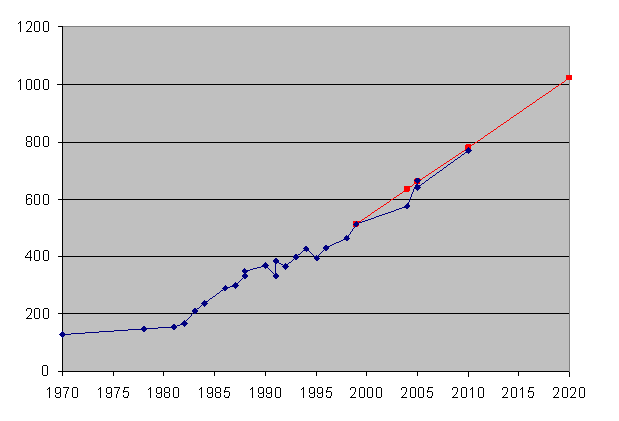
\includegraphics[scale=0.64, clip, viewport=-20 0 680 520]
                 {figures/PrognoseRSAFaktorisierungSecorvo.png}
 }
\caption{Comparison of the published factorization records (blue) and of the
predicted development (red) [Source Fox 2001; last addition 2011]}
\label{secorvo-factorization-forecast}
\end{center}
\end{figure}



\clearpage
% ++++++++++++++++++++++++++++++++++++++++++++++++++++++++++++++++++++++++++
%\vspace{4ex}
\begin{ctsquote}
    To let the possible happen, you again and again have to try the impossible.
\caption[Hermann Hesse]{Hermann Hesse\footnotemark}
\end{ctsquote}
\addtocounter{footnote}{0}\footnotetext{%
  Hermann Hesse, German/Swiss writer and Nobel Prize winner, July 2, 1877 $-$ August 9, 1962.}
% ++++++++++++++++++++++++++++++++++++++++++++++++++++++++++++++++++++++++++

\subsection{Status regarding factorization of concrete large numbers}
\label{nt:NoteFactorization} 

An exhaustive overview about the factoring records
\index{Factorization!factoring records} of composed integers using different
methods can be found on the following web pages:
\vspace{-10pt}
\begin{itemize}
\item[]
     \url{http://www.crypto-world.com} \\
     \url{http://www.tutorgig.com/ed/RSA\_number}  ~~ The RSA Factoring Challenge \\
     \url{http://en.wikipedia.org/wiki/Integer_factorization_records}\\
     \url{http://en.wikipedia.org/wiki/RSA_Factoring_Challenge}
\end{itemize}
%\footnote{%
%This site was not quite up-to-date end of May 2005: RSA-200 was missing.}

The current record (as of Nov. 2012) obtained using the GNFS method
(General Number Field Sieve) factorized a general 232 decimal digit into its
both prime factors.

\vskip +10pt
The last records\footnote{%
The 'RSA numbers' are certain large semiprime numbers (i.e., numbers with
exactly two prime factors)\index{Number!semi prime}. 
They were generated and published by the company RSA Security: In the
RSA Factoring Challenge the prime factors for these numbers are sought.\\
See \url{http://www.rsa.com/rsalabs/node.asp?id=2092}.

RSA Labs offers its challenges since the beginning of the 1990th.
The first RSA Factoring Challenge labeled the numbers, from RSA-100 
to RSA-500, according to their number of decimal digits; the second 
RSA Factoring Challenge labeled the numbers according to their number 
of binary digits. Within the second challenge cash prizes were 
offered for successful factorizations of RSA-576 to RSA-2048 (RSA-576, 
RSA-640 etc. using 64 bit steps upwards --- An exception to this is
RSA-617, which was created prior to the change in the numbering scheme).
But the RSA challenges ended ahead of time in 2007, RSA Inc. retracted
the prize.
All till now unsolved RSA challenges of RSA Labs can also be found at
the website of the cipher challenge ``MysteryTwister C3''
(\url{http://www.mysterytwisterc3.org}).
\index{MTC3}\index{Challenge}\index{Cipher challenge}\index{Crypto challenge}

The 'C numbers' originate from the Cunningham project:
\url{http://www.cerias.purdue.edu/homes/ssw/cun/}.
These are factors of Mersenne numbers, which have a very special
form. This  makes it an order of magnitude easier to factor them
as moduli of the same length build for RSA.
                          }
with factorization algorithms for composed numbers are
listed in the table~\ref{factorizationrecords}.

\begin{table}[ht]
\begin{center}
\begin{tabular}{|c|cccc|}
\hline
	& {\bf Decimal digits} & {\bf Binary digits} & {\bf Factored on} & {\bf Factored by} \\
\hline
	&&&& \\
	RSA-768 & 	232 & 768 & Dec 2010 & Thorsten Kleinjung et al. \\
	RSA-200 & 	200 & 663 & May 2005 & Jens Franke et al. \\
	RSA-640\footnotemark & 	193 & 640 & Nov 2005 & Jens Franke et al. \\
	RSA-576 & 	174 & 576 & Dec 2003 & Jens Franke et al. \\
	RSA-160 & 	160 & 530 & Apr 2003 & Jens Franke et al. \\
	RSA-155	&	155 & 512 & Aug 1999 & Herman te Riele et al. \\
	\dots &&&& \\
	C307 & 		307 & 1017 & May 2007 & Jens Franke et al. \\
	C176 & 		176 & 583 & May 2005 & Kazumaro Aoki et al. \\
	C158 & 		158 & 523 & Jan 2002 & Jens Franke et al. \\
\hline
\end{tabular}
\caption{The current factoring records (as of Nov. 2012)}    % Eyecatcher
\label{factorizationrecords}
\end{center}
\end{table} 
\footnotetext{%
A research group of the GISA solved this challenge which was awarded with
20,000 US dollar using the GNFS method. The researchers needed about five
months to divide this number into its both 320 bit long prime factors.

The researchers around Professor Jens Franke (from the University 
of Bonn, the GISA and the CWI) do not aim on getting cash prizes 
but in extending the research limits. So statements about the 
necessary length of a secure RSA modulus are more well-founded.

See \url{http://www.heise.de/newsticker/meldung/print/65957}.
}


Experiences about the ellipsed time of factorization\index{factorization}
with the open source software Pari-GP, Sage, CrypTool 1 and CrypTool 2)
can be found in ``Zeitexperimente zur Faktorisierung''.\footnote{%
R.-H. Schulz und H. Witten: ``Zeitexperimente zur Faktorisierung''. Ein Beitrag
zur Didaktik der Kryptographie'', in LogIn Heft Nr. 166/167 (2010) 113-120,
(available currently only in German)\\
\url{http://bscw.schule.de/pub/bscw.cgi/d864899/Schulz_Witten_Zeit-Experimente.pdf}
}


\vskip +20pt
%\noindent
Below these last records listed in table~\ref{factorizationrecords} are
explained in more detail\footnote{%
The two methods, GNFS and SNFS, used to do so are shortly illustrated at the 
following web pages:
\index{General Number Field Sieve (GNFS)}
\index{Special Number Field Sieve (SNFS)}
\begin{itemize}
\item[]
      \url{http://en.wikipedia.org/wiki/Special_number_field_sieve} \\
      \url{http://en.wikipedia.org/wiki/General_number_field_sieve}
\end{itemize}
\vspace{-10pt}
}:


% --------------------------------------------------------------------------
%\vskip +20pt
\paragraph*{RSA-155} \label{RSA-155} \index{RSA-155}\mbox{}

On August 22, 1999 researchers from the Netherlands found the solution of this
RSA challenge. They factorized a 155-digit number into its both 78-digit primes
(see chapter~\ref{chptSecurityParam}). 

This 512 bit RSA-155 meant to reach a kind of {\em magic} border.


% --------------------------------------------------------------------------
\vskip +20pt
\paragraph*{C158} \label{C158} \index{C158}\mbox{}
\hypertarget{C158-chap3}{}

On January 18, 2002 researchers at the German University of Bonn\footnote{%
\url{http://www.ercim.org/publication/Ercim\_News/enw49/franke.html}
}
factorized a 158-digit decimal number into its both prime factors (these are
build with 73 and 86 decimal digits) using the GNFS method (General Number
Field Sieve)\index{General Number Field Sieve (GNFS)}.

This record got much less attention within the press than the solution of
RSA-155.

The task of the researchers from Bonn was not initiated by a challenge, but
they wanted to find the last prime factors of the integer $2^{953} - 1$
(see ``Wanted List'' of the Cunningham Project\index{Cunningham project}\footnote{%
Cunningham project: \url{http://www.cerias.purdue.edu/homes/ssw/cun/}}).

The 6 smaller prime factors, already found before have been:
$$
\begin{array}{c}
3, 1907, 425796183929, \\
1624700279478894385598779655842584377, \\
3802306738549441324432139091271828121 \quad {\rm and} \\
128064886830166671444802576129115872060027.
\end{array}
$$
The first 3 factors can be easily computed\footnote{%
E.g.\ using CT1\index{CrypTool 1} via menu 
{\bf Indiv. Procedures \textbackslash{} RSA Cryptosystem \textbackslash{} 
Factorization of a Number}. \\
CT1 can factorize in a reasonable time numbers no longer than 250 bit (Numbers
bigger than 1024 bits are not accepted by CT1). CT2 is able to factorize
numbers bigger than 250 bit length.
}.
The next three prime factors were found by P.~Zimmerman\footnote{%
\url{http://www.loria.fr/~zimmerma/ecmnet}}, 
T.~Grandlund\footnote{\url{http://www.swox.se/gmp/}}
and R. Harley during the years 1999 and 2000 using the elliptic curve
factorization method.

The last remaining factor, called ``C158'', was known to be composite by
then, but its factors were not known (the following 3 lines contain one number):
$$
\begin{array}{c}
39505874583265144526419767800614481996020776460304936 \\
45413937605157935562652945068360972784246821953509354 \\
4305870490251995655335710209799226484977949442955603
\end{array}
$$
The factorization of C158 resulted in the following two 73- and 86-digit prime factors:
$$
\begin{array}{c}
3388495837466721394368393204672181522815830368604993048084925840555281177
\end{array}
$$
and
$$
\begin{array}{c}
1165882340667125990314837655838327081813101 \\
2258146392600439520994131344334162924536139.
\end{array}
$$
So now all 8 prime factors of $2^{953} - 1$ have been found.

\noindent\begin{minipage}{\textwidth}
\vspace{3ex}
Links:
\vspace{-10pt}
\begin{itemize}
\item[]   \url{http://www.loria.fr/~zimmerma/records/gnfs158}\\
          \url{http://www.crypto-world.com/FactorRecords.html}\\
          \url{http://www.crypto-world.com/announcements/c158.txt}
\end{itemize}
\end{minipage}
\vspace{12pt}



% --------------------------------------------------------------------------
\vskip +20pt
\paragraph*{RSA-160} \label{RSA-160} \index{RSA-160}\mbox{}
\hypertarget{RSA-160-chap3}{}

On January 18, 2002 researchers at the German University of Bonn\footnote{%
          \url{http://www.loria.fr/~zimmerma/records/rsa160} \\
          \url{http://www.loria.fr/~zimmerma/records/factor.html} \\
          \url{http://www.crypto-world.com/FactorWorld.html}
} 
factorized a 160-digit number into its both prime factors (these are build
with each 80 decimal digits) using the GNFS method (General Number Field
Sieve)\index{General Number Field Sieve (GNFS)}.

The  computations for the factorization of RSA-160 also took place at the 
German Information Security Agency (GISA) in Bonn.\footnote{%
Every year the GISA\index{GISA} creates a paper to describe which 
crypto algorithms are feasible to generate digital signatures according
to the German signature law -- under participation of experts from
economy and science. To review signature methods based on the
factorization problem the GISA also co-operates with researchers from the
University of Bonn.
Further information about crypto algorithms can be found on the web page of GISA:
   \url{http://www.bsi.bund.de/esig/basics/techbas/krypto/index.htm}
}

The 160-digit decimal number origins from the old challenge list of RSADSI.
This number was retracted after RSA-155 (RSA512) had been factorized 
successfully. The prime factors of RSA-160 were still unknown.
So this record of the team of Prof.\ Franke provides the solution of 
the old challenge, for which RSADSI didn't award a price anymore.

The composite number called ``RSA-160'' is (the following 3 lines contain
one number):
$$
\begin{array}{c}
215274110271888970189601520131282542925777358884567598017049 \\
767677813314521885913567301105977349105960249790711158521430 \\
2079314665202840140619946994927570407753
\end{array}
$$
The factorization of RSA-160 resulted in the following two prime factors:
$$
\begin{array}{c}
p = 45427892858481394071686190649738831 \\         
    656137145778469793250959984709250004157335359
\end{array}
$$
and
$$
\begin{array}{c}
q = 47388090603832016196633832303788951 \\
    973268922921040957944741354648812028493909367
\end{array}
$$

The calculations took place between December 2002 and April 2003.
% \vspace{12pt}
\vspace{24pt}



% --------------------------------------------------------------------------
\vskip +20pt
\hypertarget{RSA-200-chap3}{}
\paragraph*{RSA-200} \label{RSA-200} \index{RSA-200}\mbox{}

On May 9, 2005 the research group of Prof. Jens Franke at the German
University of Bonn\footnote{%
   \url{http://www.loria.fr/~zimmerma/records/rsa200}} announced,
that they achieved to factorize a 200-digit number into its both prime factors 
(these are build with each 100 decimal digits) using the GNFS method 
(General Number Field Sieve)\index{General Number Field Sieve (GNFS)}.

The composite number called ``RSA-200'' is (the following 3 lines contain
one number):
$$
\begin{array}{c}
2799783391122132787082946763872260162107044678695542853756000992932 \\
6128400107609345671052955360856061822351910951365788637105954482006 \\
576775098580557613579098734950144178863178946295187237869221823983
\end{array}
$$
The factorization of RSA-200 resulted in the following two prime factors:
$$
\begin{array}{c}
p = 35324619344027701212726049781984643686711974001976 \\         
    25023649303468776121253679423200058547956528088349
\end{array}
$$
and
$$
\begin{array}{c}
q = 79258699544783330333470858414800596877379758573642 \\
    19960734330341455767872818152135381409304740185467
\end{array}
$$

The calculations took place between December 2003 and May 2005.
The factorization done by the group around Bahr, B\"ohm, Franke, Kleinjung, 
Montgomery and te Riele lasted almost 17 months.
The operating expense of the calculations was about 120,000 
MIPS-years\footnote{%
A MIPS-year (MY) is the quantity of operations a machine can perform in one year,
if the machine constantly achieves one million integer operations per second (MIPS).
For illustration: a INTEL Pentium 100 processor achieves about 50 MIPS.
To factorize a 2048 bit module it is estimated to need about {$8.5 \cdot
 10^{40}$ MY}. }.
\vspace{24pt}



% --------------------------------------------------------------------------
\vskip +20pt
\hypertarget{RSA-768-chap3}{}
\paragraph*{RSA-768} \label{RSA-768} \index{RSA-768}\mbox{}

On December 12, 2009 the research group around Prof. Thorsten
Kleinjung\footnote{%
   \url{http://eprint.iacr.org/2010/006.pdf} \cite{nt:Kleinjung2010}
         } announced,
that they achieved to factorize a 232-digit number into its both prime factors 
(both factors have 116 decimal digits). They used the GNFS method 
(General Number Field Sieve)\index{General Number Field Sieve (GNFS)} in a
way where they did ``oversieving'' on several hundred computers
before starting the matrix step.

The composite number called ``RSA-768'' is (the following 3 lines contain
one number):
$$
\begin{array}{c}
123018668453011775513049495838496272077285356959533479219732245215172640050726\\
365751874520219978646938995647494277406384592519255732630345373154826850791702\\
6122142913461670429214311602221240479274737794080665351419597459856902143413
\end{array}
$$
The factorization of RSA-768 resulted in the following two prime factors (each with 384 bit):
$$
\begin{array}{c}
p = 3347807169895689878604416984821269081770479498371376856891\\
    2431388982883793878002287614711652531743087737814467999489
\end{array}
$$
and
$$
\begin{array}{c}
q = 3674604366679959042824463379962795263227915816434308764267\\
    6032283815739666511279233373417143396810270092798736308917
\end{array}
$$

The calculations took about 2 1/2 years.\footnote{%
This was an ``academic effort'' -- organisations with bigger resources
could do it much faster.}
\vspace{24pt}





% --------------------------------------------------------------------------
\vskip +20pt
\paragraph*{C307 / M1039} \label{C307} \index{C307} \index{M1039}\mbox{}
\hypertarget{C307-chap3}{}

In May 2007 Prof. Franke, Prof. Kleinjung (University of Bonn),
the Japanese telecommunication company NTT and Prof. Arjen Lenstra
(Polytechnical University of Lausanne) announced, that they managed to
factorize a $307$ digit decimal number into its both prime factors
with the SNFS method (Special Number Field Sieve)
\index{Special Number Field Sieve (SNFS)} within 11 months
(the two factors have 80 and 227 decimal digits).

The task of the researchers was not initiated by a challenge, but
they wanted to find the last prime factors of the Mersenne number $2^{1039}+1$
(see ``Wanted List'' of the Cunningham Project\index{Cunningham project}\footnote{%
Cunningham project: \url{http://www.cerias.purdue.edu/homes/ssw/cun/}\\
Cunningham table: \url{http://homes.cerias.purdue.edu/~ssw/cun/pmain1206}\\
The numbers in the Cunningham table have the following syntax:\\
``(2,n)-'' means $2^{n}-1$;~~~
``(2,n)+'' means $2^{n}+1$.\\
To describe the magnitude one writes $p<n>$ or $c<n>$: 
``n'' is the number of decimal digits and ``p'' and ``c'' tell,
whether the number is prime or composite.\\
$2^{1039}-1 = p7 * c307 = p7 * p80 * p227$ \\
It is explained more precisely at the page of the Cunningham project:\\
``2651+ means $2^{651} + 1$ and the size (c209 means 209 decimal digits)
of the
number which was factored.  Then come the new factor(s), the discoverer and
the method used.  Recently, only the multiple polynomial quadratic sieve
(ppmpqs), the elliptic curve method (ecm) and the number field sieve (nfs)
have been used.  `hmpqs' stands for hypercube multiple polynomial quadratic
sieve.  Under `new factors', `p90' means a 90-digit prime and `c201' is a
201-digit composite number.''.
}).\\


The number $2^{1039}-1$ consists of 3 prime factors: The smallest one, 
$p7 = 5080711$ was already known.\footnote{%
This one can also be found using CT1\index{CrypTool 1}  via menu 
{\bf Indiv. Procedures \textbackslash{} RSA Cryptosystem \textbackslash{} 
Factorization of a Number} --- with the algorithms of Brent, Williams or
Lenstra, which are ``relatively'' good to separate small factors.}


To complete this the second factor (co-divider) ``C307'' had to be factorized:
Till then it was only known, that the last remaining factor was composite,
but it was unknown, how many prime factors it had and what are the prime factors.
The following 5 lines contain one number:
$$
\begin{array}{c}
C307 =1159420574072573064369807148876894640753899791702017724986868353538\\
8224838599667566080006095408005179472053993261230204874402860435302\\
8619141014409345351233471273967988850226307575280937916602855510550\\
0425810771176177610094137970787973806187008437777186828680889844712\\
822002935201806074755451541370711023817
\end{array}
$$
The factorization of C307 resulted in the following two 80- and 2276-digit prime factors:
$$
\begin{array}{c}
p80 = 558536666199362912607492046583159449686465270184\\
      88637648010052346319853288374753
\end{array}
$$
and
$$
\begin{array}{c}
p227 = 207581819464423827645704813703594695162939708007395209881208\\
       387037927290903246793823431438841448348825340533447691122230\\
       281583276965253760914101891052419938993341097116243589620659\\
       72167481161749004803659735573409253205425523689
.
\end{array}
$$
So now the number $2^{1039}-1$ is completely factorized in its 3 prime factors.

\noindent\begin{minipage}{\textwidth}
\vspace{3ex}
Links:
\vspace{-10pt}
\begin{itemize}
\item[]]   \url{http://www.loria.fr/~zimmerma/records/21039-}\\
          \url{http://www.crypto-world.com/announcements/m1039.txt}\\
          \url{http://www.crypto-world.com/FactorAnnouncements.html}\\
          \url{http://www1.uni-bonn.de/pressDB/jsp/pressemitteilungsdetails.jsp?detailjahr=2007&detail=160}
\end{itemize}
\end{minipage}






% --------------------------------------------------------------------------
\vskip +70pt
\paragraph*{Size of factorized numbers compared to primality proven numbers}
\mbox{}

As you notice the factorized compound numbers built of 2 prime factors are
much smaller than the especially structured numbers, for which primality 
tests\index{Primality testing} are able to decide whether these numbers are prime 
or not (see chapters~\ref{search_for_very_big_primes},~\ref{primality_tests}
and \ref{spezialzahlentypen}). 

% be_2005_UPDATEN_if-new-mersenne-prime-appears % Eyecatcher_neue-Mersenne
Length of the current world records in decimal notation:

$$ [RSA{-}768~number] ~~\longleftrightarrow{}~~ [47th ~known~Mersenne~prime] $$
$$ 232 ~~ \longleftrightarrow{} ~~ 17,425,170 ~~~~~$$
$$ [see~table~\ref{factorizationrecords}] ~~\longleftrightarrow{}~~ [see~table~\ref{L_n_Largest_Known-Primes}] ~~~~~~~~~~~~~~~~$$



% --------------------------------------------------------------------------
\vskip +60pt
\subsection{Further current research about primes and factorization}
\label{FactorizationResearch}
Prime numbers are part of very many topical research areas in number theory
and computer science. Progress made with factorization is bigger than was
estimated 5 years ago -- this is not only due to faster computers but
also new mathematical knowledge.

The security of the RSA algorithm is based on the empirical observation
that factoring large numbers is a hard problem. A module $n$ (typically,
1024 bit) can be easily constructed as the product of two large primes $p$,
$q$ (typically, 500$-$600 bit each), by calculating $n=pq$. However, it is
a hard problem to extract $p$, $q$ from $n$.  Without knowing $p$ or $q$,
the private key cannot be calculated.

Thus, any progress in efficiency of factorizing large integers will effect the
security of the RSA. As a consequence, the underlying primes $p$, $q$ and,
thus, the module n (1024 bit as of today) have to be increased. In case of a
quantum leap in factorization, the RSA algorithm might be compromised.


% --------------------------------------------------------------------------
\vskip +20pt
%\paragraph*
\subsubsection{Bernstein's paper and its implication on the
               security of the RSA algorithm}
\label{RSABernstein} \index{Factorization!factorization problem}\mbox{}
In his paper ``Circuits for integer factorization: a proposal'' 
(\url{http://cr.yp.to/djb.html}, published November 2001,
D.~J.\ Bernstein \cite{nt:Bernstein2001} addresses the problem of
factorizing large integers. Therefore, his results are of relevance from a
RSA point of view.  As a main result Bernstein claims that the
implementation of the General Number Field Sieve algorithm (GNFS)
 \index{General Number Field Sieve (GNFS)} can be improved to factor, with
the same effort as before, integers with three times more digits.

We note that the definition of \emph{effort} is a crucial point: Bernstein
claims that effort is the product of time and costs of the machine
(including the memory used). The gist of the paper lies in the fact that he
can reduce a big part of factorizing to sorting. Using Schimmler's scheme,
sorting can be optimized by massive parallel computing.  At the end of
section 3 Bernstein explains this effect: The costs of $m^2$ parallel
computers with a constant amount of memory is a constant times $m^2$.  The
costs of a computer with a single processor and memory of size $m^2$ is
also of the order of $m^2$, but with a different constant factor.  With
$m^2$ processors in parallel, sorting of $m^2$ numbers (with Schimmler's
scheme) can be achieved in time $m$, while a $m^2$-memory computer needs
time of the order of $m^2$. Decreasing memory and increasing the number of
processors, the computing time can be reduced by a factor $1/m$ without
additional effort in terms of total costs.  In section 5 it is said that
massive parallel computing can also increase efficiency of factorizing
using Lenstra's elliptic-curve-method (a search algorithm has costs that
increase in a quadratic square manner instead of cubically).

We note that all results achieved so far are asymptotic results. This means
that they only hold in the limit n to infinity. Unfortunately, there is no
upper limit for the residual error (i.e. the difference between the real
and the asymptotic value) for finite n --- a problem which has already been
addressed by the author. As a consequence, one cannot conclude whether the
costs (in the sense of Bernstein) for factorizing 1024$-$2048-bit RSA modules
can be significantly reduced.

There is no doubt that Bernstein's approach is innovative. However, the
reduction of computing time under constant costs comes along with a massive
use of parallel computing --- a scenario which seems not to be realistic
yet. For example, formally 1 sec computing time on one machine and
1/1,000,000 sec time parallel computing time on 1,000,000 machines might
have same costs.  In reality, it is much harder to realize the second
situation, and Bernstein does not take into account the fixed costs, in
particular for building a network between all these computers.

Although distributed computing over a large network might help to overcome
this problem, realistic costs for data transfer have to be taken into
account --- a point which was not addressed in Bernstein's proposal.

As long as there is neither (low cost) hardware nor a distributed computing
approach (based on Bernstein's ideas), there should not be a problem for
RSA. It has to be clarified from which magnitude of n on Bernstein's method
could lead to a significant improvement (in the sense of the asymptotic
result). 

Arjen Lenstra, Adi Shamir et. al. analyzed the paper of Bernstein
\cite{nt:Lenstra2002}.  In summary they expect a factorization improvement on
how much longer the bit length of the keys could be with a factor of 1.17
(instead of factor 3 as proposed by Bernstein).

The abstract of their paper ``Analysis of Bernstein's Factorization
Circuit'' says:

``... Bernstein proposed a circuit-based implementation of the matrix
step of the number field sieve factorization algorithm. We show that under
the non-standard cost function used in [1], these circuits indeed offer an
asymptotic improvement over other methods but to a lesser degree than
previously claimed: for a given cost, the new method can factor integers
that are 1.17 times larger (rather than 3.01).  We also propose an improved
circuit design based on a new mesh routing algorithm, and show that for
factorization of 1024-bit integers the matrix step can, under an optimistic
assumption about the matrix size, be completed within a day by a device
that costs a few thousand dollars.  We conclude that from a practical
standpoint, the security of RSA relies exclusively on the hardness of the
relation collection step of the number field sieve.''

RSA Security\footnote{\url{http://www.rsasecurity.com/}} concludes in its
analysis of the Bernstein paper \cite{nt:RSA Security 2002} from April, 8 2002
also -- as expected -- that RSA is still not compromised.

This is still an ongoing discussion.

When this section was written (June 2002) nothing was publicly known about, how
far there exist implementations of his theoretical onsets and how much
financing there was for his research project.

\vskip +12pt
\noindent\begin{minipage}{\textwidth}
Links:
\vspace{-10pt}
\begin{itemize}
  \item[] \url{http://cr.yp.to/djb.html}\\
          \url{http://www.counterpane.com/crypto-gram-0203.html\#6} \\
          \url{http://www.math.uic.edu}
\end{itemize}
\end{minipage}


% --------------------------------------------------------------------------
\vskip +20pt
%\paragraph*
\subsubsection{The TWIRL device} \label{TWIRLDevice} \index{TWIRL device}
%\mbox{}

In January 2003 Adi Shamir and Eran Tromer from the Weizmann Institute of Science published a preliminary draft called {\em ``Factoring Large Numbers with the TWIRL Device''} raising concerns about the security of key sizes till 1024 bits \cite{nt:Shamir2003}. 

Their abstract summarizes their results very well: ``The security of the RSA
cryptosystem depends on the difficulty in factoring large integers. The best
current factoring algorithm is the Number Field Sieve (NFS), and its most
difficult part is the sieving step. In 1999 a large distributed computation
involving thousands of workstations working for many months managed to factor a
512-bit RSA key, but 1024-bit keys were believed to be safe for the next 15-20
years. In this paper we describe a new hardware implementation of the NFS
sieving step ... which is 3-4 orders of magnitude more cost effective than the
best previously published designs ... . Based on a detailed analysis of all the
critical components (but without an actual implementation), we believe that the
NFS sieving step for 1024-bit RSA keys can be completed in less than a year with
a \$10M device, and that the NFS sieving step for 512-bit RSA keys can be
completed in less than ten minutes with a \$10K device. Coupled with recent
results about the difficulty of the NFS matrix step ... this raises some
concerns about the security of these key sizes.''

A detailed explanation from these two authors also can be found in the
RSA Laboratories CryptoBytes \cite{nt:Shamir2003a}.

The 3-page article in the DuD issue of June 2003 \cite{nt:Weis2003} contains
a very good explanation, how the attack using the Generalized Number Field
Sieve (GNFS) \index{General Number Field Sieve (GNFS)} works and which 
progress is made, to factorize numbers.
At GNFS we can distinguish 2 general steps: 
The sieve step (relation collecting) and the matrix reduction.
Besides the sieve step is highly parallelizable, it dominates the overall
calculation burden. Shamir and Tromer haven't built a TWIRL device yet,
but the estimated costs of 10 till 50 million Euro (in order to factorize
a 1024-bit number) is not prohibitive for secret agencies or big criminal
organizations, because the ``costs for a single espionage satellite is
estimated e.g.\ to be several billion USD''. The authors therefore
recommend, to get as soon as possible rid of today used sensible RSA, 
Diffie-Hellman or ElGamal keys up to 1024 bit and to use then keys of at
least 2048 bit length.
The planned TCPA/Palladium hardware \index{Palladium} will use 2048-bit
RSA keys!

So recommendations like the ones from the GISA (German Information Security Agency) to use higher key lengths are very valid.


% --------------------------------------------------------------------------
\vskip +20pt
%\paragraph*
\subsubsection{``Primes in P'': Primality testing is polynomial}
\label{PrimesinP} \index{Primality testing}%\mbox{}

In August 2002 the three Indian researchers M. Agrawal, N. Kayal and N. Saxena published the paper {\em ``PRIMES in P''} about a new primality testing algorithm called AKS\index{AKS} \cite{nt:Agrawal2002}. 
They discovered a polynomial\index{Polynomial} time deterministic algorithm for determining if a number is prime or not.

The importance of this discovery is that it provides number theorists with new insights and opportunities for further research. Lots of people over centuries have been looking for a polynomial time test for primality, and this result is a major theoretic breakthrough. It shows that new results can be generated from already known facts.

But even its authors note that other known algorithms may be faster (for example ECPP). The new algorithm works on any integer. For example the GIMPS project uses the Lucas-Lehmer primality test which takes advantage of the special properties of Mersenne numbers. This makes the Lucas-Lehmer test much faster, allowing to test numbers with millions of digits while general purpose algorithms are limited to numbers with a few thousand digits.

\noindent Current research results on this topic can be found at:
\vspace{-10pt}
\begin{itemize}
  \item[] \url{http://www.mersenne.org/} \\
          \url{http://fatphil.org/maths/AKS/} Original paper in English\\
          \href{http://ls2-www.cs.uni-dortmund.de/lehre/winter200203/kt/material/primes.ps}{\tt http://ls2-www.cs.uni-dortmund.de/lehre/winter200203/kt/material/primes.ps} \\% \url... created overfull \hbox
	  \hspace*{2em}Good explanation in German by Thomas Hofmeister.
\end{itemize}
\vskip +10 pt


% --------------------------------------------------------------------------
% \vskip +20pt
\newpage
\subsubsection{Shared Primes: Modules with common prime factors}
\label{nt_Shared-Primes} \index{Prime!Shared}%\mbox{}
%~\ref{nt_Shared-Primes}, page~\pageref{nt_Shared-Primes}

The RSA algorithm for public-key cryptography is based on the presumed difficulty of factoring large bi-prime integers, the factoring problem. However, as pointed out in Lenstra et al \cite{nt:Lenstra2012} it is possible, given a set of moduli, to factor some of them by finding shared primes. This way the factoring problem is bypassed using a simple greatest common divisor (gcd) operation. It is no trivial task to extract common shared primes and to factor the according moduli efficiently for a very big number of given moduli (several millions).

Using the gcd only works if the RSA keys were not generated randomly. Taking into consideration the significance of strong cryptographic keys it is important to verify that all keys were generated following the principle of true randomness \cite{nt:Esslinger2012}. 

When Lenstra et al published their paper \cite{nt:Lenstra2012} in Feb. 2012, they did not publish the source code. However, soon afterwards the source code of a similar program was published at the CrypTool website\footnote{%
\url{http://www.cryptool.org/en/ctp-dokumentation-en/361-ctp-paper-rsa-moduli}
%\url{http://www.cryptool.org/de/ctp-dokumentation-de/361-ctp-paper-rsa-moduli}
}
in Python and C++, and at the page used by \cite{nt:Heninger2012}\footnote{\url{https://www.factorable.net/}
}.
The fastest code known to me comes with \cite{nt:Heninger2012}.

These applications find all shared factors that may exist, given a finite set of moduli -- even if this set includes millions of moduli. Such an application enables system administrators to test their own RSA keys. 

The quite naive way to find all shared factors would be to compare each modul with all other moduli which has a complexity growing quadratically with the number of moduli.
A very efficient method using trees for comparing all gcd pairs is based on a publication of Dan Bernstein in 2005 \cite{nt:Bernstein2005}. Bernstein uses a precalculation which leads to the product of all moduli. It's another example showing how helpful precalculations can be to break cryptographic systems (another famous example are rainbow tables used to find the origin of a hash value \cite{nt:Oechslin2003}).


The following Sage sample shows the very different run times when calculating a gcd and a factorization. The section after this sample will explain the essential part of the method used in \cite{nt:Heninger2012}: Using the trees accelerates the calculation of the gcd pairs a lot.

The Sage sample~\ref{nt_sagesample_Compare-Runtime-gcd-factoring} shows that multiplication of factors, dividing a modul with a known factor, or calculating the gcd is very fast. However, factoring moduli steeply increases with longer moduli. Even the relatively small moduli used in this example show this: The smaller modul (69 decimal digits, 228 bits) took 76 seconds, while the bigger one (72 decimal digits, 239 bits) took almost 217 seconds.

In addition, the operations multiplication, divsion and gcd show big differences in runtime when the used operands are very different in size.

% Just to show the origin of the used primes
% sage: factor (2^211-1)
% 15193 * 60272956433838849161 * 3593875704495823757388199894268773153439
%
% sage: factor (2^214-1)
% 3 * 643 * 84115747449047881488635567801 * 162259276829213363391578010288127
\begin{sagecode}
\begin{Verbatim}%
[fontsize=\footnotesize,fontshape=tt]

# Multiplication
sage: 3593875704495823757388199894268773153439 * 84115747449047881488635567801
302301541122639745170382530168903859625492057067780948293331060817639

sage: 3593875704495823757388199894268773153439 * 162259276829213363391578010288127
583139672825572068433667900695808357466165186436234672858047078770918753


# Division
sage: time 302301541122639745170382530168903859625492057067780948293331060817639 / 
           3593875704495823757388199894268773153439
Wall time: 0.00 s
84115747449047881488635567801

sage: time 583139672825572068433667900695808357466165186436234672858047078770918753 / 
           3593875704495823757388199894268773153439
Wall time: 0.00 s
162259276829213363391578010288127


# Calculate gcd
sage: time gcd (583139672825572068433667900695808357466165186436234672858047078770918753,
                302301541122639745170382530168903859625492057067780948293331060817639)
Wall time: 0.00 s
3593875704495823757388199894268773153439


# Factorize
sage: time factor (583139672825572068433667900695808357466165186436234672858047078770918753)
Wall time: 217.08 s
162259276829213363391578010288127 * 3593875704495823757388199894268773153439

sage: time factor (302301541122639745170382530168903859625492057067780948293331060817639)
Wall time: 76.85 s
84115747449047881488635567801 * 3593875704495823757388199894268773153439

\end{Verbatim}
\caption{Comparing the runtime of calculating a gcd and performing a factorization}
\label{nt_sagesample_Compare-Runtime-gcd-factoring}
\end{sagecode}



\clearpage
\section*{Efficient computing of all gcd pairs and explanation of the formula used}

The paper "Mining Your Ps and Qs: Detection of Widespread Weak Keys in Network Devices"~\cite{nt:Heninger2012} explains the algorithm how the gcd's of every pair of RSA moduli are calculated efficiently.

First the product $P$ of all moduli $m_{i}$ is calculated using a product tree. Then a remainder tree is build modulo the squares of the moduli. Then the gcd's of a defined modul $m_{i}$ and of the remainders $z_{i}$ divided by this defined modul are calculated. 

This is visualized in Figure \ref{Figure_Bernstein_Computing-all-pairs-GCDs} which is a copy from \cite{nt:Heninger2012} (where the moduli are called $N_{i}$
instead of $m_{i}$:
\begin{figure}[ht]
\begin{center}
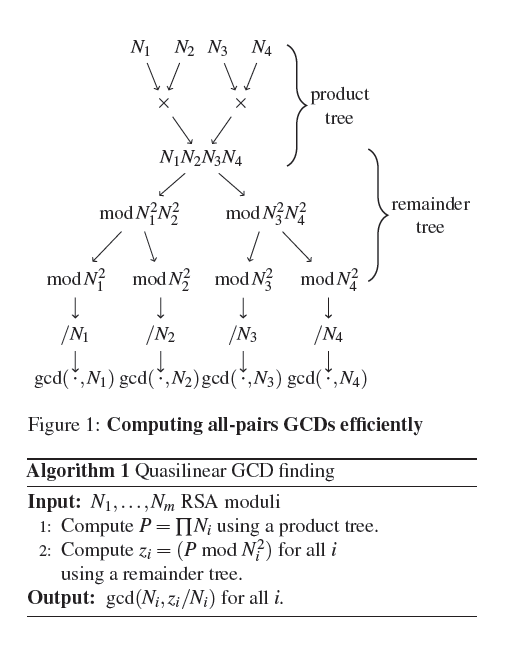
\includegraphics[scale=0.7]{figures/Bernstein_Computing-all-pairs-GCDs.png}
\caption{Algorithm and Figure to compute all gcd pairs efficiently} 
\label{Figure_Bernstein_Computing-all-pairs-GCDs}
\end{center}
\end{figure}


The paper~\cite{nt:Heninger2012} explains well \textit{how} the algorithm works, but not as well \textit{why}. The product $P$ of all moduli is a very big number, even compared to a single modul. Without the simplifications from the remainder tree you would go the following way: Calculate $gcd_{i} = gcd( P / m_{i},  m_{i}) $ for all i. Compare each $gcd_{i} \ne 1$ with all other $gcd_{j} \ne 1$ with  $j \ne i$. If two gcd's are the same, then their moduli share a factor.

As it's very slow to calculate this for numbers with such a big difference in size, the remainder tree is used. Despite it seems to consist of more steps it's a huge simplification.

Within the remainder tree you get -- at the end -- $(P \bmod ({m_{i}^{2}}) ) / m_{i}$ for all $i$.\footnote{%
It would not make sense to calculate $(P \bmod m_{i} ) / m_{i}$
as $(P \bmod m_{i} )$ is always $= 0$.

Sample with very small moduli:\\
$ m_{1} = 2*3 = 6;~~~ m_{2} = 2*7 = 14;~~~ P=6*14=84 $\\
$ P \bmod m_{1} = 84 \bmod 6 = 0;~~~ P \bmod {m_{1}^{2}} = 84 \bmod 36 = 12 $\\
$ P \bmod m_{2} = 84 \bmod 14 = 0;~~~ P \bmod {m_{2}^{2}} = 84 \bmod 196 = 84 $\\
$gcd_{1} = gcd(12/6, 6) = gcd(2, 6) = 2 $\\
$gcd_{2} = gcd(84/14, 14) = gcd(6, 14) = 2 $

The way the tree is structured it also would not make sense to first divide and then do the modulo calculation, as making the division first would lead just to the given moduli but in reversed order.

It also would not make sense to calculate $(P \bmod ({m_{i}^{3}}) ) / {m_{i}^{2}})$ as this is only additional effort with no improvement.
}

The main remaining question now is: Why does $gcd((P \bmod {m_{i}^{2}})/ m_{i}, m_{i})$ deliver the same result as $gcd( P / m_{i}, m_{i})$ ?
We prove that this identity is correct.

P represents here the product of all moduli, and $m_{i}$ represents any
arbitrary modulus.%\mbox{}\\\mbox{}\\

$$gcd((P \bmod {m_{i}^{2}})/ m_{i}, m_{i})~~~  \overset{!}{=}  ~~~gcd( P / m_{i}, m_{i})$$
$ \Longleftrightarrow $~~~\footnote{According to Euklid's algorithm the following identities are true:
\mbox{}\\
$gcd((P \bmod {m_{i}^{2}})/ m_{i}, m_{i})=gcd((P \bmod {m_{i}^{2}})/ m_{i} \bmod{m_{i}}, m_{i})$ \mbox{}\\
$gcd( P / m_{i}, m_{i})=gcd( P / m_{i} \bmod{m_{i}}, m_{i})$\mbox{}
}

$$gcd(((P \bmod {m_{i}^{2}})/ m_{i}) \bmod {m_{i}}, m_{i})~~~  \overset{!}{=}  ~~~gcd( (P / m_{i}) \bmod {m_{i}}, m_{i})$$
$ \Longleftrightarrow $~~~\footnote{The gcd's are equal if both their first arguments are equal.
}

$$((P \bmod {m_{i}^{2}})/ m_{i}) \bmod {m_{i}}~~~  \overset{!}{=}  ~~~ (P / m_{i}) \bmod {m_{i}}$$
$ \Longleftrightarrow $~~~\footnote{The following transformations are all equalities.
}

$$(P \bmod{m_{i}^{2}})/ m_{i} - P / m_{i} \equiv 0   \bmod{m_{i}}~~~ \Leftrightarrow ~~~  m_{i} ~~ | ~~ ((P \bmod{m_{i}^{2}})/ m_{i} - P / m_{i})$$~~~\footnote{%
According to the definition of modulus and division it is:\\
$a \bmod{b} ~~ \Longleftrightarrow ~~ a - b * \lfloor a/b \rfloor$\\
So $P \bmod{m_{i}^{2}}$ can be written as $ P-m_{i}^{2} \lfloor P/m_{i}^{2} \rfloor$.
}

$$ m_{i} ~~ | ~~ ((P-m_{i}^{2}* \lfloor P/m_{i}^{2} \rfloor - P))/m_{i}$$~~~\footnote{%
$P$ reduces itself, the exponent in the $m_{i}$ enumerator is simplified with the  $m_{i}$ denominator.
}

$$ m_{i} ~~ | ~~ (m_{i}* \lfloor P/m_{i}^{2} \rfloor)$$

As this is true, we can conclude that the two gcds are equivalent.

% yyyyyyyyyyyyyyyyyyyyyyyyyyy

% S�tze und Links:
% https://en.wikipedia.org/wiki/Greatest_common_divisor
% https://de.wikipedia.org/wiki/Gr%C3%B6%C3%9Fter_gemeinsamer_Teiler


%TODO: Wohl durch das verschobene Sage-Beispiel wirkt das \newpage vor dem ff. Kapitel nicht!


% ++++++++++++++++++++++++++++++++++++++++++++++++++++++++++++++++++++++++++
% \vskip +40 pt
\newpage
\begin{ctsquote}
It is our choices, that show what we truly are, far more than our abilities.
\caption[Joanne K. Rowling]{Joanne K. Rowling\footnotemark}\index{Rowling, Joanne}
\end{ctsquote}

\addtocounter{footnote}{0}\footnotetext{Joanne K. Rowling, ~``Harry Potter and the Chamber of Secrets'', Bloomsbury, 1998, 
last chapter ``Dobby's reward'', p.~245, by Dumbledore.}

%\begin{quote}
%{\em Joanne K. Rowling}\footnote{Joanne K. Rowling, ~``Harry Potter and the Chamber of Secrets'', Carlsen, 1998, 
%last chapter ``Dobby's reward'', p.~343.}:\\
%It is our choices, that show what we truly are, far more than our abilities.
%\end{quote}

% ++++++++++++++++++++++++++++++++++++++++++++++++++++++++++++++++++++++++++
\section{Applications of asymmetric cryptography using numerical examples}

The results of modular arithmetic are used extensively in \index{Cryptography!modern} modern cryptography. Here we will provide a few examples from 
cryptography using small\footnote{In the RSA procedure, we call numbers ``small'' if the bit lengths are much less than $1024$ bits (i.e. $308$ decimal points). In practice,
$1024$ bits is currently considered the minimum length for a secure RSA modul.} numbers.

Enciphering a text entails applying a function (mathematical operation) to a character string (number) to generate a 
different number. Deciphering entails reversing this function, in other words using the distorted image that the function 
has created from the plaintext in order to restore the original image. For example, the sender could take the plaintext 
$M$ of a confidential message and add a secret number, the key $S$, to obtain the ciphertext $C$:
$$C = M + S.$$
The recipient can reconstruct the plaintext by reversing this operation, in other words by subtracting $S$:
$$M = C - S.$$
Adding $S$ reliably makes the plaintext impossible to read. However, this encryption is rather weak, because all an 
interceptor needs to do to calculate the key is obtain a plaintext and the associated ciphertext
$$S = C - M,$$
and can then read any subsequent messages encrypted using $S$. \\
The essential reason for this is that subtraction is just as simple an operation as addition. 


% --------------------------------------------------------------------------
\hypertarget{OneWayFunktion2}{}%
\subsection{One way functions}\index{One way function}
\label{OneWayFunktion2}%
If the key is to be impossible to determine even with knowledge of both the 
plaintext and the ciphertext, we need a function that is, on the one hand, 
relatively easy to calculate -- we don't want to have problems encrypting 
messages. On the other hand, the inverse function should exist (otherwise 
information would be lost during encryption), but should be de facto 
incalculable.

What are possible candidates for such a {\bf one way function}? We could take multiplication rather than addition, 
but even primary school children know that the inverse function, division, is only slightly more difficult than multiplication 
itself. We need to go one step higher in the hierarchy of calculation methods. It is still relatively simple to calculate the 
power of a number, but the corresponding two reverse functions -- {\em taking roots} (find $b$ in the equation $a = b^c$  when $a$ 
and $c$ are known) and {\em calculating logarithms} (find $c$ in the above equation when $a$ and $b$ are known) are so complicated 
that pupils normally do not learn them at school.

Although a certain structure can still be recognised for addition and multiplication, raising numbers to the power of 
another or calculating exponentials totally mixes up all the numbers. Knowing a few values of the function doesn't tell 
us much about the function as a whole (in contrast to addition and multiplication).


% --------------------------------------------------------------------------
\vskip +10 pt
\subsection{The Diffie-Hellman key exchange protocol}
\index{Diffie, Whitfield} 
\index{Hellman, Martin} 
\index{Key agreement (key exchange)!Diffie-Hellman}
\index{Diffie-Hellman}

Whitfield Diffie, Martin E. Hellman and Ralph Merkle developed this DH key 
exchange protocol in Stanford in 1976.\footnote{%
  With CT1\index{CrypTool 1} this exchange protocol has been
  visualized: You can execute the single steps with concrete numbers using 
  menu {\bf Indiv. Procedures \textbackslash{} Protocols
  \textbackslash{} Diffie-Hellman Demonstration}.\\
  In JCT\index{JCrypTool} you can find it in the default perspective
  via the menu item {\bf Visuals \textbackslash{} Diffie-Hellman
  Key Exchange (EC)}.
}

Alice and Bob\footnote{Bob\index{Bob} and Alice\index{Alice} are the default
names used for the two authorized participants in a protocol (see
\cite[p. 23]{nt:Schneier1996nt}).
} use a one way function to obtain a key $S$, the session key, for subsequent
correspondence. This is then a secret that is only known to the two of them.
Alice selects a random number $a$ and keeps it secret. She applies a one way
function to $a$ to calculate the number $A = g^a$ and sends it to Bob. He does
the same, by selecting a secret random number $b$, calculating $B = g^b$ and
sending it to Alice. The number $g$ is random and can be publicly known.
Alice applies the one way function together with her secret number $a$ to
$B$, while Bob does the same with his secret number $b$ and the received
number $A$.

The result $S$ is the same in each case because the one way function is
commutative: $(g^a)^b = (g^b)^a$. But even Bob cannot reconstruct Alice's
secret number $a$ from the data available to him, while Alice cannot
determine Bob's secret number $b$. And a perpetrator who knows $g$ and
has intercepted both $A$ and $B$ cannot use this knowledge to 
determine $a, b$ or $S$.

\vskip +10 pt
\input{figures/DH-en.latex}
\vskip +20 pt

\noindent {\bf Procedure:}\par  %\par bewirkt Zeilenumbruch
\nopagebreak
\noindent Alice and Bob want to negotiate a secret session key $S$ via
a channel that may be intercepted. 
\begin{itemize}
\item[{\bf 1.}] They select a prime number $p$ and a random number $g$ and exchange this information openly.
\item[{\bf 2.}] Alice now selects $a$, a random number less than $p$ and keeps it secret.

                Similarly, Bob selects $b,$ a random number less than $p$ and keeps it secret.
\item[{\bf 3.}] Alice now calculates $A \equiv g^a {\rm ~(mod~} p)$.\\
                Bob calculates $B \equiv g^b {\rm ~(mod~} p)$.
\item[{\bf 4.}] Alice sends the result $A$ to Bob.\\
                Bob sends the result $B$ to Alice.
\item[{\bf 5.}] In order to now determine the session key to be used by both,
                they both separately raise the respective results they have
                received to the power of their secret random number modulo $p$.
                This means: 
\begin{itemize}
    \item[-] Alice calculates $S \equiv B^a {\rm ~(mod~} p)$ and
    \item[-] Bob calculates $S \equiv A^b {\rm ~(mod~} p)$.
\end{itemize}
\end{itemize}
Even if a spy intercepts $g, p$, and the interim results $A$ and $B$, he cannot
use these in order to determine the used session key used -- due to the
difficulty of calculating the discrete logarithm\footnotemark.
\footnotetext{%
Further details about
the\index{Logarithm problem!discrete}\index{Discrete logarithm}
\hyperlink{HT-Discrete-Logarithm-as-Basis}{discrete logarithm problem}
can be found in chapter~\ref{L-Discrete-Logarithm-as-Basis}.
}

\vskip + 5pt
\noindent We will now use an example with (unrealistically) small numbers to illustrate this.
\vskip +1em

\begin{example}{ using small numbers:}
\begin{itemize}
\item[{\bf 1.}] Alice and Bob select $g = 11, p = 347$.
\item[{\bf 2.}] Alice selects $a = 240$, Bob selects $b = 39$ and they keep $a$ and $b$ secret.
\item[{\bf 3.}] Alice calculates $A \equiv g^a \equiv 11^{240}  \equiv 49 {\rm ~(mod~} 347).$\\
                Bob calculates $B \equiv g^b \equiv 11^{39} \equiv 285 {\rm ~(mod~} 347).$
\item[{\bf 4.}] Alice sends Bob:   $A \equiv 49$,\\
                Bob sends Alice: $B \equiv 285$.
\item[{\bf 5.}] Alice calculates $B^a \equiv 285^{240} \equiv 268 {\rm ~(mod~} 347),$\\
                Bob calculates $A^b \equiv   49^{39} \equiv 268 {\rm ~(mod~} 347).$
\end{itemize}
Alice and Bob can now communicate securely using their shared session key. Even if spies were to intercept everything 
transferred via the connection:
$g = 11, p = 347, A = 49$ and $B = 285$, they would not be able to calculate the secret key.
\end{example}

\newpage
\begin{remark}{:}\\
In this example using such small numbers, it is easily possible to calculate the discrete
logarithms, but with large numbers the discrete logarithm\index{Discrete logarithm}
problem\footnote{%
You can use Sage to determine the discrete logarithm $x$ that solves the
equation $11^x \equiv 49 \pmod{347}$ (here for Alice)\index{Sage}:
\texttt{discrete\_log(mod(49, 347), mod(11, 347))}. The returned value
is $67$.\\
Such number theoretic tasks can also be solved using other
tools like PariGP\index{Pari-GP}, LiDIA\index{LiDIA}, BC\index{BC} or
Mathematica\index{Mathematica}
(see the list of web sites in the appendix at the end of this chapter):\\
- Pari-GP: \texttt{znlog(Mod(49,347),Mod(11,347))}.\\
- LiDIA:   \texttt{dl(11,49,347)}.\\
- Mathematica: The general Solve function delivers the {em tdep message} ``The equations
  appear to involve the variables to be solved for in an essentially non-algebraic way''.\\
- Mathematica: {\tt MultiplicativeOrder[11, 347, 49]}.\\
All deliver the result $67$.
}${}^,$\footnote{%
Why have the functions delivered the value $67$ for the discrete
logarithm\index{Discrete logarithm} of Alice rather than $240$ which Alice
selected as exponent $a$?\\
The discrete logarithm is
the smallest natural exponent that solves the equation 
$11^x \equiv 49 \pmod{347}$. Both $x = 67$ and $x = 240$ (the number
selected in the example) satisfy the equation and can therefore be
used to calculate the session key: 
$285^{240} \equiv 285^{67} \equiv 268 \pmod{347}$.
If Alice and Bob
had selected a primitive root\index{Primitive root} modulo $p$ as base $g$, then for every
remainder from the set $\{1, 2, \dots, p-1 \}$ there is exactly one
exponent from the set $\{0, 1, \dots, p-2 \}$. \\
\indent As an aside, there are $172$ different primitive roots modulo $347$,
$32$ of which are prime (not necessary). Since the number $11$
selected for $g$ in the example is not a primitive root\index{Primitive root} of $347$, the
remainders do not take all values from the set $\{1, 2, \dots, 346 \}$. 
Thus, for a particular remainder there may be more than one exponent
or even no exponent at all in the set $\{0, 1, \dots, 345 \}$ that
satisfies the equation.\\
With the relevant Sage\index{Sage} commands you find:\\
\texttt{is\_prime(347)=True}, \texttt{euler\_phi(347)=346}, \texttt{gcd(11,347)=1} and 
\texttt{multiplicative\_order(mod(11, 347))=173}.

\begin{tabular}{|c|c|l|}
\hline
i  & $11^i \bmod 347$ & \\
\hline
      0  &          1   &  \\
      1  &         11   &  \\                                     
      2  &        121   &  \\                                     
      3  &        290   &  \\                                     
     67  &         49   & searched exponent \\                    
    172  &        284   &  \\                                                  
    173  &          1   &= multiplicative order of $11^i \bmod 347$ \\ 
    174  &         11   &  \\                                                     
    175  &        121   &  \\                                     
    176  &        290   &  \\                                     
    240  &         49   & searched exponent \\
\hline
\end{tabular}
\vskip +6 pt

\noindent Further information can be found in
chapter~\ref{nt:AppArith3a2} ``\nameref{nt:AppArith3a2}''.
}
is extremely difficult to solve.
\end{remark}

\noindent To get the discrete logarithms, here we need to calculate:\\
For Alice: $11 ^ x \equiv 49 {\rm ~(mod~}347)$, that means $\log_{11}(49) {\rm ~(mod~}347).$\\
For Bob: $11 ^ y \equiv 285 {\rm ~(mod~}347)$, that means $\log_{11}(285){\rm ~(mod~}347)$.



% ++++++++++++++++++++++++++++++++++++++++++++++++++++++++++++++++++++++++++
\newpage
\hypertarget{Chapter_ElementaryNT_12}{}
\section[The RSA procedure with actual numbers]{The RSA procedure with actual numbers\footnotemark}
\footnotetext{%
    \index{Sage}%
    \index{Nguyen, Minh Van }%
    Additional material: Minh Van Nguyen, ``Number Theory and the RSA
    Public Key Cryptosystem'', 2009. An introductory tutorial on using
    Sage to study elementary number theory and public key
    cryptography. A didactically very clear article about some basic
    number theory and Sage usage.\\
    \url{http://nguyenminh2.googlepages.com/sage_numtheory-rsa.pdf}.
}
\label{rsaconcrete}\index{RSA}

\begin{ctsquote}
``Games are Nature's way of preparing us to face difficult realities. Are you finally ready to face reality, Sergeant?''
\caption[Daniel Suarez]{Daniel Suarez\footnotemark}\index{Suarez, Daniel}
\end{ctsquote}
\addtocounter{footnote}{0}\footnotetext{Daniel Suarez, ``Daemon'', Dutton Adult, 2010,
Chapter 45, ``Respawning'', p. 610, Sobol.}

Having described above \hyperlink{RSA}{how the RSA procedure works}, we will now work through the steps using actual, but small, numbers.


% --------------------------------------------------------------------------
\subsection{RSA with small prime numbers and with a number as message}

Before applying the RSA procedure to a text, we will first demonstrate it
directly using a single number as message.\footnote{%
   Using CT1\index{CrypTool 1} you can solve this with the menu {\bf Indiv.
   Procedures \textbackslash{} RSA Cryptosystem \textbackslash{} RSA Demonstration}.
}
\begin{itemize}
\item[{\bf 1.}] Let the selected prime numbers be $p=5$ and $q=11$. \\
Thus, $n=55$ and $J(n)=(p-1)*(q-1)=40$.
\item[{\bf 2.}] $e = 7$ ($e$ should\footnote{%
                See footnote~\ref{foot:Selection-of-e} on page
                \pageref{foot:Selection-of-e}.} lie between $11$ and $39$,
                and must be relatively prime to $40$).
\item[{\bf 3.}] $d = 23$ (since $23*7 \equiv 161 \equiv 1{\rm ~(mod~} 40)$),
    \begin{itemize}
    \item[] $\rightarrow$ Public key of the recipient:  $(55, 7),$
    \item[] $\rightarrow$ Private key of the recipient: $(55, 23).$
    \end{itemize}
\item[{\bf 4.}] Let the message be the number $M = 2$ (so no division into blocks is required).
\item[{\bf 5.}] Encryption: $C \equiv 2^7 \equiv 18 {\rm ~(mod~}55).$
\item[{\bf 6.}] The ciphertext is simply the number $C = 18$ (we therefore do not need to divide it into blocks).
\item[{\bf 7.}] Decryption: 
        $M \equiv 18^{23} \equiv 18^{(1+2+4+16)} \equiv 18*49*36*26 \equiv 2 {\rm ~(mod~}55).$
\end{itemize}


We will now apply the RSA procedure to a text, first using the upper case alphabet ($26$ characters), then using the entire ASCII character set as the basis for the messages.


% --------------------------------------------------------------------------
\subsection[RSA with slightly larger primes and an upper-case message]{RSA with slightly larger primes and a text of upper case letters}
\label{rsaex2}

We have the text ``ATTACK AT DAWN'', and the characters are coded according to
table~\ref{alphacode}.\footnote{%
Using CT1\index{CrypTool 1} you can solve this with the menu {\bf Indiv. Procedures
\textbackslash{} RSA Cryptosystem \textbackslash{} RSA Demonstration}.
This is also described in the tutorial/scenario in CT1's online help [Options,
specify alphabet, number system, block length\index{Block length} 2 and decimal
representation].
}

\begin{table}[ht]
\begin{center}
\begin{tabular}{|c|l||c|l|}
\hline
Character & Numerical value & Character & Numerical value \\
\hline
\hline
Blank    & 0   & M  & 13 \\
A        & 1   & N    & 14 \\ 
B        & 2   & O    & 15 \\ 
C        & 3   & P    & 16 \\  
D        & 4   & Q    & 17 \\ 
E        & 5   & R    & 18 \\ 
F        & 6   & S    & 19 \\  
G        & 7   & T    & 20 \\  
H        & 8   & U    & 21 \\ 
I        & 9   & V    & 22 \\   
J       & 10   & W    & 23 \\  
K       & 11   & X    & 24 \\ 
L       & 12   & Y    & 25 \\
&              & Z    & 26 \\
\hline
\end{tabular}
\end{center}
\hypertarget{Grossbuchstaben-Alphabet}{}    
\caption{Capital letters alphabet}\index{Capital letters alphabet}
\label{alphacode}
\end{table}
\vskip +20 pt

\noindent {\bf Key generation (steps 1 to 3)}:\\
{\bf 1.} $p=47, q=79$ $( n= 3713; ~J(n) = (p-1)*(q-1)=3588).$ \\
{\bf 2.} $e = 37$ ($e$ should\footnote{%
                See footnote~\ref{foot:Selection-of-e} on page
                \pageref{foot:Selection-of-e}.} lie between $79$ and $3587$,
                and must be relatively prime to $3588$). \\
{\bf 3.} $d=97$ (since $e*d=1{\rm ~mod~}J(n); 37*97 \equiv 3589
                        \equiv 1{\rm ~(mod~}3588) \;$).\footnote{%
 How to compute $d = 97$ using the {\em extended} gcd algorithm is shown
 in appendix~\ref{nt:NumberTheory_Appendix_GCD}} \\

\noindent {\bf 4. Encryption}:\\
{\tt
\begin{tabular}{rcccccccccccccccccccc}
{\rm Text:} & A & T & T & A & C & K & & A & T &  & D & A & W & N \\
{\rm Number:} & 01 & 20 & 20 & 01 & 03 & 11 & 00 & 01 & 20 & 00 & 04 & 01 & 23 & 14
\end{tabular}
}

\noindent This $28$-digit number is divided into $4$-digit parts
(because $2626$ is still smaller than $n=3713$):\\
{\tt 0120 2001 0311 0001 2000 0401 2314}

\label{SrcArith4a}
\noindent All 7 parts are encrypted using: $C \equiv M^{37}{\rm ~(mod~}3713)$:\footnote{%
  See chapter~\ref{nt:AppArith4a} ``\nameref{nt:AppArith4a}''
  for source code to do RSA encryption using Sage. \\
  You can also encrypt the message with CT1\index{CrypTool 1} via the menu path 
  {\bf Indiv. Procedures \textbackslash{} RSA Cryptosystem \textbackslash{}
  RSA Demonstration}.
} \\
{\tt 1404 2932 3536 0001 3284 2280 2235}

\noindent {\bf 5. Decryption}: \\
Ciphertext: {\tt 1404 2932 3536 0001 3284 2280 2235 }

\noindent This $28$-digit number is divided into $4$-digit parts.

\noindent All 7 parts are decrypted using:  $M \equiv C^{97}{\rm ~(mod~}3713)$: \\
{\tt 0120 2001 0311 0001 2000 0401 2314}

\noindent The 2-digit numbers are transformed into capital letters and blanks.

\noindent Using the selected values it is easy for a cryptanalyst\index{Cryptanalysis}
to derive the secret values from the public 
parameters $n=3713$ and $e=37$ by revealing that $3713 = 47 * 79$.

\noindent If $n$ is a $768$-bit number, there is, according to present knowledge,
little chance of this.


% --------------------------------------------------------------------------
\subsection{RSA with even larger primes and a text made up of ASCII characters}

In real life, the ASCII alphabet is used to code the individual characters
of the message as $8$-bit numbers.

\noindent The idea for this task\footnote{%
Using CT1\index{CrypTool 1} you can solve this via the menu path {\bf Indiv. Procedures
\textbackslash{} RSA Cryptosystem \textbackslash{} RSA Demonstration}.
} 
is taken from the example in \cite[p. 271]{nt:Eckert2003}\index{Eckert 2003}.

\noindent Coded in decimal notation, the text ``RSA works!'' is as follows: \\
{\tt
\begin{tabular}{rcccccccccccccccccccc}
{\rm Text:} & R & S & A &   & w & o & r & k & s & ! \\
{\rm Number:} & 82 & 83 & 65 & 32 & 119 & 111 & 114 & 107 & 115 & 33 
\end{tabular} } % \tt

\noindent We will work through the example in 2 variants. The steps 1 to 3 are common for both.
\par
\noindent {\bf Key generation (steps 1 to 3)}:
\label{SrcArith4b} \\
{\bf 1.} $p=503,~q=509 \quad (n= 256,027; \; J(n)=(p-1)(q-1)=255,016=2^3*127*251)$.\footnote{%
  See chapter~\ref{nt:AppArith4b} ``\nameref{nt:AppArith4b}''
  for the source code to factorize the number $J(n)$ using Sage.
  Using CT1\index{CrypTool 1} you can solve this with the 
  {\bf Indiv. Procedures \textbackslash{} RSA Cryptosystem \textbackslash{} 
  Factorization of a Number}.} \\
{\bf 2.} $e=65,537$ \\
\strut\quad\ ($e$ should\footnote{%
                See footnote~\ref{foot:Selection-of-e} on page
                \pageref{foot:Selection-of-e}.}
                lie between $509$ and $255,015$, and must\footnote{%
       $e$ cannot, therefore, be $2, 127$ or $251$
       ($65,537 = 2^{16}+1$) ($255,016 = 2^{3}*127*251$).\\
       In real life, $J(n)$ is not factorized but rather the Euclidean
       algorithm is used for the selected e to guarantee that
       ${\rm gcd}(e,J(n))=1$.
                 } be relatively prime to $255,016$).\\
{\bf 3.} $d=231,953$ \\
\strut\quad\ (since $e \equiv d^{-1}{\rm ~mod~}J(n): ~65,537*231,953 \equiv 15,201,503,761 \equiv 1
{\rm ~(mod~}255,016)$).\footnote{Other possible combinations of $(e,d)$ include: $(3, 170,011)$, $(5, 204,013)$, $(7, 36,431)$.}


% --------------------------------------------------------------------------
\subsection*{Variant 1: All ASCII characters are en-/decrypted separately (no blocks\index{Block length} are formed).}

{\bf 4. Encryption}:\\
{\tt
\begin{tabular}{rcccccccccccccccccccc}
{\rm Text:} & R & S & A &   & w & o & r & k & s & ! \\
{\rm Number:} & 82 & 83 & 65 & 32 & 119 & 111 & 114 & 107 & 115 & 33 
\end{tabular} } % \tt

\noindent The letters are not combined!\footnote{For secure procedures we need large numbers that assume -- as far as possible -- all 
values up to $n-1$. If the possible value set for the numbers in the message is too small, even large prime numbers 
cannot make the procedure secure.  An ASCII character is represented by $8$ bits. If we want larger values we must 
combine several numbers. Two characters need $16$ bits, whereby the maximum value that can be represented is $65536$. 
The modulus $n$ must then be greater than $2^{16} = 65536$. This is applied in variant 2.
When the numbers are combined, the leading zeros are kept in binary notation (just as if we were to write all numbers with $3$ 
digits in decimal notation above and were then to obtain the sequence 
{\tt 082 083,  065 032, 119 111,  114 107,  115 033}).}
\label{SrcArith4c}\\
Each character is encrypted using: $C = M^{65,537} {\rm ~(mod~} 256,027)$:\footnote{%
  See chapter~\ref{nt:AppArith4c} ``\nameref{nt:AppArith4c}''
  for the source code for RSA exponentiation using Sage.
} \\
{\tt
\begin{tabular}{lllll}
212984 & 025546 & 104529 & 031692 & 248407 \\
100412 & 054196 & 100184 & 058179 & 227433\\
\end{tabular} }

\noindent {\bf 5. Decryption}:\\
Ciphertext: 

{\tt
\begin{tabular}{lllll}
212984 & 025546 & 104529 & 031692 & 248407 \\
100412 & 054196 & 100184 & 058179 & 227433\\
\end{tabular} } 

\noindent Each character is decrypted using: $M \equiv C^{231,953}{\rm ~mod~}256,027$: \\
{\tt 82 83 65 32 119 111 114 107 115 33}


% --------------------------------------------------------------------------
\subsection*{Variant 2: The ASCII characters are en-/decrypted two at a time as blocks.}

In variant 2 the block formation is done in two different sub-variants: (4./5. and 4'./5'.).

{\tt
\begin{tabular}{rcccccccccccccccccccc}
{\rm Text:} & R & S & A &   & w & o & r & k & s & ! \\
{\rm Number:} & 82 & 83 & 65 & 32 & 119 & 111 & 114 & 107 & 115 & 33 
\end{tabular} } % \tt

\noindent {\bf 4. Encryption:}\\
Blocks are formed\footnote{\vskip +3 pt \tt \begin{tabular}{ll@{ }l@{ }l}
single character& binary representation  && decimal representation\\
01010010, 82 & 01010010 01010011 & = &21075 \\
01010011, 83 & \\
01000001, 65 & 01000001 00100000 & = &16672  \\
00100000, 32  \\
01110111, 119 & 01110111 01101111 & = &30575 \\
01101111, 111 \\ 
01110010, 114 & 01110010 01101011 & = &29291 \\
01101011, 107 \\
01110011, 115 & 01110011 00100001 & = &29473 \\
00100001, 33: 
\end{tabular}} (each ASCII character is encoded into a 8 digit binary number below):\\
{\tt 21075 16672 30575 29291 29473}\footnote{%
Using CT1\index{CrypTool 1} you can solve this with the menu {\bf Indiv. Procedures
\textbackslash{} RSA Cryptosystem \textbackslash{} RSA Demonstration} 
with the following options: all 256 ASCII characters, b-adic,
block length\index{Block length} 2 and decimal representation.
}

\label{SrcArith4d}
\noindent Each block is encrypted using: $C \equiv M^{65,537}{\rm ~(mod~}256,027)$:\footnote{%
  See chapter~\ref{nt:AppArith4d} ``\nameref{nt:AppArith4d}''
  for the source code for RSA exponentiation using Sage.
} \\
{\tt 158721 137346 37358 240130 112898}

\noindent {\bf 5. Decryption:} \\
Ciphertext:\\
{\tt 158721 137346 37358 240130 112898}

\noindent Each block is decrypted using: $M \equiv C^{231,953}{\rm ~(mod~}256,027)$: \\
{\tt 21075 16672 30575 29291 29473}


% Conversion:
%   Divide each block into $2$ numbers using binary.
%   Then convert each number to ASCII characters.

\noindent {\bf 4'. Encryption:} \\
Blocks are formed: (each ASCII character is encoded into a 3 digit decimal number below):\\
 {\tt 82083 65032 119111 114107 115033}\footnote{The RSA encryption works correctly with the
modulus $n=256.027$ because each ASCII block of two characters will be encoded into a number that is smaller or equal than
the number $255,255$.  } 

\label{SrcArith4e}
\noindent Each block is encrypted using: $C \equiv M^{65,537}{\rm ~(mod~}256,027)$:\footnote{%
  See chapter~\ref{nt:AppArith4e} ``\nameref{nt:AppArith4e}''
  for the source code for RSA exponentiation using Sage.
} \\
{\tt 198967 051405 254571 115318 014251}

\noindent {\bf 5'. Decryption:} \\
Ciphertext:\\
 {\tt 198967 051405 254571 115318 014251}

\noindent Each block is decrypted using: $M \equiv C^{2473}{\rm ~(mod~}67,519)$: \\
{\tt 82083 65032 119111 114107 115033}


% --------------------------------------------------------------------------
\newpage
\subsection{A small RSA cipher challenge (1)} \index{RSA!cipher challenge}

The task is taken from \cite[Exercise 4.6]{nt:Stinson1995}\index{Stinson 1995}:
The pure solution has been published by Prof. Stinson.\footnote{%
\url{http://www.cacr.math.uwaterloo.ca/~dstinson/solns.html} or
\url{http://bibd.unl/~stinson/solns.html}
}
However, it is not the result that is important here but rather the
individual steps of the solution, that is, the explanation of the 
cryptanalysis\index{Cryptanalysis}.\footnote{The method of solving the
problem is outlined in the scenario of the online help to
CT1\index{CrypTool 1} and in the presentation on the CT website.
If anyone sends us a well prepared exact method of solving the problem,
we would be pleased to include it in the documentation.}

Two samples of RSA ciphertext are presented in Tables~\ref{stinson1}\footnote{%
The numbers of this table can be worked with via Copy and Paste.
}
and \ref{stinson2}\footnote{%
The numbers of this table are in the online help of CT1\index{CrypTool 1}
in the chapter ``Example illustrating the RSA demonstration''.
}. 
Your task is to decrypt them. The public parameters of the system are 

\noindent $n = 18,923$ and $e = 1261$ (for Table~\ref{stinson1}) and \\
\noindent $n = 31,313$ and $e = 4913$ (for Table~\ref{stinson2}). 

This can be accomplished as follows. First, factor $n$ (which is easy
because it is so small). Then compute the exponent $d$ from $J(n)$, and,
finally, decrypt the ciphertext. Use the square-and-multiply
\index{Square and multiply} algorithm to exponentiate modulo $n$. 

In order to translate the plaintext back into ordinary English text, you
need to know how alphabetic characters are ``encoded'' as elements in
$\mathbb{Z}_n$. Each element of $\mathbb{Z}_n$ represents three alphabetic
characters as in the following examples:

{\tt \begin{tabular}{lll}
DOG & $\mapsto$ & $3 * 26^2 + 14 * 26 + 6= 2398$ \\
CAT & $\mapsto$ & $2 * 26^2 + 0 * 26 + 19 = 1371$ \\
ZZZ & $\mapsto$ & $25 * 26^2 + 25 * 26 + 25 = 17,575$. 
\end{tabular} }

You will have to invert this process as the final step in your program.

The first plaintext was taken from ``The Diary of Samuel Marchbanks'', by Robertson Davies, 1947, and the second was 
taken from ``Lake Wobegon Days'', by Garrison Keillor, 1985.


\begin{table}[ht]
\begin{center}
{\tt 
\begin{tabular}{llllllll}
12423 & 11524  & 7243  & 7459 & 14303  & 6127 & 10964 & 16399 \\
 9792 & 13629 & 14407 & 18817 & 18830 & 13556  & 3159 & 16647 \\
 5300 & 13951    & 81  & 8986  & 8007 & 13167 & 10022 & 17213 \\
 2264   & 961 & 17459  & 4101  & 2999 & 14569 & 17183 & 15827 \\
12693  & 9553 & 18194  & 3830  & 2664 & 13998 & 12501 & 18873 \\
12161 & 13071 & 16900  & 7233  & 8270 & 17086  & 9792 & 14266 \\
13236  & 5300 & 13951  & 8850 & 12129  & 6091 & 18110  & 3332 \\
15061 & 12347  & 7817  & 7946 & 11675 & 13924 & 13892 & 18031 \\
 2620  & 6276  & 8500   & 201  & 8850 & 11178 & 16477 & 10161 \\
 3533 & 13842  & 7537 & 12259 & 18110    & 44  & 2364 & 15570 \\
 3460  & 9886  & 8687  & 4481 & 11231  & 7547 & 11383 & 17910 \\
12867 & 13203  & 5102  & 4742  & 5053 & 15407  & 2976  & 9330 \\
12192    & 56  & 2471 & 15334   & 841 & 13995 & 17592 & 13297 \\
 2430  & 9741 & 11675   & 424  & 6686   & 738 & 13874  & 8168 \\
 7913  & 6246 & 14301  & 1144  & 9056 & 15967  & 7328 & 13203 \\
  796   & 195  & 9872 & 16979 & 15404 & 14130  & 9105  & 2001 \\
 9792 & 14251  & 1498 & 11296  & 1105  & 4502 & 16979  & 1105 \\
   56  & 4118 & 11302  & 5988  & 3363 & 15827  & 6928  & 4191 \\
 4277 & 10617   & 874 & 13211 & 11821  & 3090 & 18110    & 44 \\
 2364 & 15570  & 3460  & 9886  & 9988  & 3798  & 1158  & 9872 \\
16979 & 15404  & 6127  & 9872  & 3652 & 14838  & 7437  & 2540 \\
 1367  & 2512 & 14407  & 5053  & 1521   & 297 & 10935 & 17137 \\
 2186  & 9433 & 13293  & 7555 & 13618 & 13000  & 6490  & 5310 \\
18676  & 4782 & 11374   & 446  & 4165 & 11634  & 3846 & 14611 \\
 2364  & 6789 & 11634  & 4493  & 4063  & 4576 & 17955  & 7965 \\
11748 & 14616 & 11453 & 17666   & 925    & 56  & 4118 & 18031 \\
 9522 & 14838  & 7437  & 3880 & 11476  & 8305  & 5102  & 2999 \\
18628 & 14326  & 9175  & 9061   & 650 & 18110  & 8720 & 15404 \\
 2951   & 722 & 15334   & 841 & 15610  & 2443 & 11056  & 2186 
\end{tabular} } % tt
\end{center}
\caption{RSA ciphertext A}
\label{stinson1}
\end{table}

\begin{table}[ht]
\begin{center}
{\tt 
\begin{tabular}{llllllll}
 6340  & 8309 & 14010  & 8936 & 27358 & 25023 & 16481 & 25809 \\
23614  & 7135 & 24996 & 30590 & 27570 & 26486 & 30388  & 9395 \\
27584 & 14999  & 4517 & 12146 & 29421 & 26439  & 1606 & 17881 \\
25774  & 7647 & 23901  & 7372 & 25774 & 18436 & 12056 & 13547 \\
 7908  & 8635  & 2149  & 1908 & 22076  & 7372  & 8686  & 1304 \\
 4082 & 11803  & 5314   & 107  & 7359 & 22470  & 7372 & 22827 \\
15698 & 30317  & 4685 & 14696 & 30388  & 8671 & 29956 & 15705 \\
 1417 & 26905 & 25809 & 28347 & 26277  & 7897 & 20240 & 21519 \\
12437  & 1108 & 27106 & 18743 & 24144 & 10685 & 25234 & 30155 \\
23005  & 8267  & 9917  & 7994  & 9694  & 2149 & 10042 & 27705 \\
15930 & 29748  & 8635 & 23645 & 11738 & 24591 & 20240 & 27212 \\
27486  & 9741  & 2149 & 29329  & 2149  & 5501 & 14015 & 30155 \\
18154 & 22319 & 27705 & 20321 & 23254 & 13624  & 3249  & 5443 \\
 2149 & 16975 & 16087 & 14600 & 27705 & 19386  & 7325 & 26277 \\
19554 & 23614  & 7553  & 4734  & 8091 & 23973 & 14015   & 107 \\
 3183 & 17347 & 25234  & 4595 & 21498  & 6360 & 19837  & 8463 \\
 6000 & 31280 & 29413  & 2066   & 369 & 23204  & 8425  & 7792 \\
25973  & 4477 & 30989                               
\end{tabular} } % tt
\end{center}
\caption{RSA ciphertext B}
\label{stinson2}
\end{table}


% --------------------------------------------------------------------------
\clearpage
\subsection{A small RSA cipher challenge (2)}
\index{RSA!cipher challenge}

The following task is a corrected version from the book written by Prof. Yan 
\cite[Example 3.3.7, p. 318]{nt:Yan2000}\index{Yan 2000}.
However, it is not the result that is important here but rather the
individual steps of the solution, that is, the explanation of the
cryptanalysis\index{Cryptanalysis}.\footnote{%
The method of solving the problem is outlined in the scenario of the online
help to CT1\index{CrypTool 1} and in the CrypTool presentation.
If anyone sends us a well prepared exact method of solving the problem,
we would be pleased to include it in the documentation.
}

There are three tasks with completely different degrees of difficulty here.
In each case we know the ciphertext 
and the public key $(e,n)$:
\begin{itemize}
\item[{\bf (a)}] Known plaintext: \index{Attack!known plaintext} find the secret key $d$ using the additionally known original message.
\item[{\bf (b)}] Ciphertext-only: \index{Attack!ciphertext-only} find $d$ and the plaintext.
\item[{\bf (c)}] Calculate the RSA modulus, in other words factorization (with no knowledge of the message). \index{Factorization!factorization problem}
\end{itemize}

%\newpage
$n = 63978486879527143858831415041, ~e = 17579$

Message\footnote{%
The numbers of this table are in the online help of CT1\index{CrypTool 1}
in the chapter ``Example illustrating the RSA demonstration''.
}:

{\tt
\begin{tabular}{l}
1401202118011200, \\
1421130205181900, \\
0118050013010405, \\
0002250007150400 
\end{tabular} } % tt

Cipher:

{\tt
\begin{tabular}{l}
45411667895024938209259253423, \\
16597091621432020076311552201, \\
46468979279750354732637631044, \\
32870167545903741339819671379
\end{tabular} } % tt
\vskip +8pt

\begin{remark}{:}\\
The original message consisted of a sentence containing $31$ characters (coded
with the capital letters alphabet \index{Capital letters alphabet} from
section~\ref{rsaex2}).  Each group of $16$ decimal numbers is then combined to
form one number (the last number is filled with zeros). These numbers are
raised to the power of $e$.
\end{remark}

When you decrypt the message you must fill the calculated numbers with leading
zeros in order to obtain plaintext.

This needs to be stressed because the type of padding is extremely important
during implementation and standardization for interoperable algorithms.








% ---------------------------------------------------------------------------
% ---------------------------------------------------------------------------

% ++++++++++++++++++++++++++++++++++++++++++++++++++++++++++++++++++++++++++
\newpage
\hypertarget{nt:NumberTheory_Appendix_GCD}{}
\section[Appendix: gcd and the two algorithms of Euclid]
        {Appendix: The greatest common divisor (gcd) of whole numbers
         and the two algorithms of Euclid\footnotemark}
\footnotetext{%
    \index{NT, Learning Tool for Number Theory}%
    \index{Educational tool NT}%
With the educational tool for number theory {\bf NT} you can see\\
a) how Euklid's algorithm calculates the gcd (learning unit 1.3, pages 14-19/21) and \\
b) how Euklid's enhanced algorithm finds the multiplicative inverse
   (learning unit 2.2, page 13/40).\\
NT can be called in CT1\index{CrypTool 1} via the menu path
{\bf Indiv. Procedures \textbackslash{} Number Theory Interactive
\textbackslash{} Learning Tool for Number Theory}.
See appendix~\ref{s:appendix-Learn-NT}.\\
    CT2\index{CrypTool 2} contains Euklid's extended algorithm within the
    tutorial ``{\bf World of Primes} --> Number Theory --> Number-theoretic
    functions: Extended Euklid''  bxxxxxxxxxxxxxxxxxxxxxxxxxx .
}
\label{nt:NumberTheory_Appendix_GCD}
% \addcontentsline{toc}{section}{Appendix A: gcd of whole numbers and the two
%  algorithms of Euclid}\index{Euclidean algorithm!extended}
\index{Euclidean algorithm!extended}
\index{gcd}

%%%\begin{enumerate}
%%%\item
The greatest common divisor of two natural numbers $a$ and $b$ is an important value
that can be calculated very quickly. Here we make use of the fact that if a number
$c$ divides the numbers $a$ and $b$ (i.e. there exists an $a'$ and a $b'$ such that
$a = a'*c$ and $b = b'*c$), then $c$ also divides the remainder $r$ of $a/b$.
In short notion we can write: If $c$ divides $a$ and $b$ it follows that 
$c$ divides $r =  a - \lfloor a/b \rfloor * b$.\footnote{\label{nt_Gauss-Klammer}%
The Gauss\index{Gauss bracket} bracket  $\lfloor x \rfloor $ of a real number $x$
is defined via: $\lfloor x \rfloor $ is the next integer less or equal $x$.\\
See footnote~\ref{nt_Gauss-Funktion} on page~\pageref{nt_Gauss-Funktion}.
%aaaaaaaaaaaaaaaaaaaaaaa
}

As the latter statement is valid for each common divisor $c$ of $a$ and $b$ it
follows that: $$gcd(a,b) = gcd(a - \lfloor a/b \rfloor * b, b).$$
Using this information, the algorithm for calculating the gcd of two numbers can be
written as follows (in pseudo code):

\begin{verbatim}
INPUT: a,b != 0
1. if ( a < b ) then  x = a; a = b; b = x; // Swap a and b (a > b)
2. a = a - int(a/b) * b                    // a is smaller than b, the 
                                           // gcd(a, b) is unchanged 
3. if ( a != 0 ) then goto 1.              // a falls after each step and 
                                           // the algorithm ends when a==0.
OUTPUT "gcd(a,b) = " b    // b is the gcd of the original a and b
\end{verbatim}

%%%\item 
Also further relationships can be derived from the gcd:
For this, we need the set of equations for $a$ and $b$:
\begin{eqnarray*}
 a & = & 1*a + 0*b \nonumber \\
 b & = & 0*a + 1*b, \nonumber
\end{eqnarray*}
or, in matrix notation:
$$ \left(\begin{array}{c}a \\ b\end{array}\right) = 
   \left(\begin{array}{cc} 1 & 0 \\ 0 & 1 \end{array}\right) *
   \left(\begin{array}{c} a \\ b \end{array} \right).$$

We summarize this information in the extended matrix:
$$\left(\begin{array}{cccc} a & | & 1 & 0 \\ b & | & 0 & 1 \end{array} \right)$$
If we apply the above gcd algorithm to this matrix, we obtain the
{\em extended Euclid algorithm} which can be used to calculate the multiplicative inverse: 
\index{Euclidean algorithm!extended}

\newpage
\noindent {\tt INPUT:} $a,b \not= 0$
\begin{itemize}
  \item[\tt 0.] $x_{1,1} := 1, x_{1,2} := 0, x_{2,1} := 0, x_{2,2} := 1$
  \item[\tt 1.] $ \left(\begin{array}{cccc} a & | & x_{1,1} & x_{1,2} \\ b & | & x_{2,1} & x_{2,2} \end{array} \right) := 
           \left(\begin{array}{cc} 0 & 1  \\ 1 & - \lfloor a/b \rfloor * b \end{array} \right)*
           \left(\begin{array}{cccc} a & | & x_{1,1} & x_{1,2} \\ b & | & x_{2,1} & x_{2,2} \end{array} \right).$
  \item[\tt 2.] {\tt if (b != 0) then goto 1.}
\end{itemize}

{\tt OUTPUT:} ``gcd$(a,b) = a*x +b*y$: '', ``gcd$(a,b) =$ '' $b$,
              ``$x = $'' $x_{2,1}$, ``$y = $'' $x_{2,2}$

\noindent Since this algorithm only performs linear transformations, the same equations always apply
\begin{eqnarray*}
 a & = & x_{1,1}*a + x_{1,2}*b \nonumber \\
 b & = & x_{2,1}*a + x_{2,2}*b, \nonumber
\end{eqnarray*}
We get the extended gcd equation at the end of the algorithm\footnote{%
By termination of the gcd algorithm, the program variables $a$ and $b$ contain
the values $a= 0$ and $b=gcd(a,b)$. Please keep in mind, that the program
variables are different to the numbers $a$ and $b$ and that they are only
relevant for the scope of the algorithm.}:
$$gcd(a,b) = a*x_{2,1} + b*x_{2,2}.$$

\begin{example}{:}\\
Using the extended gcd we can determine for $e = 37$ the multiplicative inverse
number $d$ to modulo $3588$ (i.e. $37*d \equiv 1 {\rm ~(mod~} 3588$)): 

{\tt 0.}
 $ \left(\begin{array}{cccc} 3588 & | & 1 & 0 \\ 37 & | & 0 & 1 \end{array} \right)$ 
 
{\tt 1.}
 $ \left(\begin{array}{cccc} 37 & | & 1 & 0 \\ 36 & | & 0 & -96 \end{array} \right) = 
   \left(\begin{array}{cc} 0 & 1  \\ 1 & - (\lfloor 3588/36 \rfloor = 96) * 37 \end{array} \right)*
   \left(\begin{array}{cccc} 3588 & | & 1 & 0 \\ 37 & | & 0 & 1 \end{array} \right).$
   
{\tt 2.}
 $ \left(\begin{array}{cccc} 36 & | & 1 & -96 \\ 1 & | & -1 & 97 \end{array} \right) = 
   \left(\begin{array}{cc} 0 & 1  \\ 1 & - (\lfloor 37/36 \rfloor = 1) * 36 \end{array} \right)*
   \left(\begin{array}{cccc} 37 & | & 1 & 0 \\ 36 & | & 0 & -96 \end{array} \right).$
   
{\tt 3.}
 $ \left(\begin{array}{cccc} {\bf 1} & | & {\bf -1} & {\bf 97} \\ 0 & | & 37 & -3588 \end{array} \right) = 
   \left(\begin{array}{cc} 0 & 1  \\ 1 & - (\lfloor 36/1 \rfloor = 36) * 1 \end{array} \right)*
   \left(\begin{array}{cccc} 36 & | & 1 & -96 \\ 1 & | & -1 & 97 \end{array} \right).$\\

\vskip + 12pt
\noindent {\tt OUTPUT:} \\
gcd($37,3588) = a*x + b*y$: \\
gcd($37,3588$) = 1, $x = -1$, $y=97$.

\noindent Thus 
\begin{enumerate}

\item $37$ and $3588$ are relatively prime ($37$ has an inverse modulo $3588$).
      \index{Number!co-prime}

\item $37*97 = (1 * 3588) + 1$ in other words $37*97 \equiv 1 {\rm ~(mod~} 3588).$ \\
      and therefore the number $97$ is the multiplicative inverse to $37$ modulo $3588$.

\end{enumerate}

\end{example}
% End of gcd and the two algorithms of Euclid.



% ++++++++++++++++++++++++++++++++++++++++++++++++++++++++++++++++++++++++++
\newpage
\hypertarget{nt:NumberTheory_Appendix_B}{}
\section{Appendix: Forming closed sets}
\label{nt:NumberTheory_Appendix_B}{}

The property of closeness\index{Closeness} within a set is always defined in
relation to an operation.
The following shows how to construct the ``closed set'' $G$ with respect to
the operation $+ {\rm ~(mod~} 8)$ for a given initial set $G_0$:

\begin{eqnarray*}
G_0 & = & \{ 2, 3 \} {\rm ~~--- addition~of~the~numbers~in~} G_0
{\rm ~determines~further~numbers:} \nonumber \\
    & &    2 + 3 \equiv 5{\rm ~(mod~}8) = 5 \nonumber \\
    & &    2 + 2 \equiv 4{\rm ~(mod~}8) = 4 \nonumber \\
    & &    3 + 3 \equiv 6{\rm ~(mod~}8) = 6 \nonumber \\ 
G_1 & = & \{ 2, 3, 4, 5, 6 \} {\rm ~~--- addition~of~the~numbers~in~} G_1
{\rm ~determines:}\nonumber \\
    & &    3 + 4 \equiv 7{\rm ~(mod~}8) = 7 \nonumber \\
    & &    3 + 5 \equiv 8{\rm ~(mod~}8) = 0 \nonumber \\
    & &    3 + 6 \equiv 9{\rm ~(mod~}8) = 1 \nonumber \\ 
G_2 & = & \{ 0, 1, 2, 3, 4, 5, 6, 7 \} {\rm ~~--- addition~of~the~numbers~in~} G_2
{~does~not~extend~the~set!} \nonumber \\
G_3 & = & G_2 {\rm ~~--- we~say:~} G_2 {\rm~is~closed~for~addition~~(mod~}8). \nonumber 
\end{eqnarray*}
% End of forming a closed set.



% ++++++++++++++++++++++++++++++++++++++++++++++++++++++++++++++++++++++++++
\vskip +60pt
\hypertarget{nt:NumberTheory_Appendix_C}{}
\section{Appendix: Comments on modulo subtraction}
\label{nt:NumberTheory_Appendix_C}{}

Comment on subtraction modulo 5: $2 - 4 = -2 \equiv 3{\rm ~mod~}2$.\\
It is therefore not true that $-2 = 2 mod 5$ !

People often make the mistake of equating this.
You can show this clearly if you place the permutation $(0, 1, 2, 3, 4)$
in $\mathbb{Z}_5$, for example from $-11$ to $+11$, over the range of
numbers in $\mathbb{Z}$.

\vskip +10 pt
\input{figures/line-en.latex}



% ++++++++++++++++++++++++++++++++++++++++++++++++++++++++++++++++++++++++++
\newpage
\hypertarget{NumberTheory_Appendix_D}{}
\section[Appendix: Base representation of numbers, estimation of length of digits]
        {Appendix: Base representation and base transformation of numbers,
         estimation of length of digits}
\label{l:NumberTheory_Appendix_D}{}

For a given number $z$ one may ask how to represent such a number. In general
we use representations like $z = 2374$ or $z = \sqrt{2}$. The second number
consists of an infinite number of digits and therefore it can never be
described precisely by the first representation. You can get around this problem
by writing the number symbolically. But if you have to write it in digits,
the number must be rounded.

We represent numbers usually in the decimal system (base 10). Computers
are working with the binary representation of numbers --- only for the
display numbers are represented in decimal or sometimes hexadecimal (base 16)
form.

This appendix describes how to generate arbitrary base representations of
any positive integer and how to determine the number of required digits
via the logarithm function.


\subsection*{$b$-adic sum representation of positive integers}

Given base $b$, each positive integer $z$ can be represented as a $b$-adic
sum  $$ z = a_nb^n + a_{n-1}b^{n-1} + \cdots + a_1b + a_0, $$ where
$a_i \in \{0, 1, \dots, b-1\}, \; i=0,1,\dots, n$ are called {\em digits}.

For this sum, it follows that:\\
1) For arbitrary digits $a_0, a_1, \dots, a_n$ it is:
   $b^{n+1} > a_nb^n + a_{n-1}b^{n-1} + \cdots + a_1b + a_0$.\\
2) There exist digits $a_0, a_1, \dots, a_n$
   ~(namely $a_i = b-1$ for $i=0, \dots, n$), following that  
   $b^{n+1} -1 \le a_nb^n + a_{n-1}b^{n-1} + \cdots + a_1b + a_0$.\\
(Using these inequalities it can be shown that each positive integer can be
represented by a $b$-adic sum).

By writing the digits $a_na_{n-1} \cdots a_1a_0$ in a row directly after each
other (without the $b^i$) the usual writing for numbers comes to hand.

\begin{example}{:}\\
Base $b = 10$: $10278 =  1\cdot10^4 +  0\cdot 10^3 + 2\cdot 10^2 + 7\cdot 10^1 + 8$\\
Base $b = 16$: $FE70A = 15\cdot16^4 + 14\cdot 16^3 + 7\cdot 16^2 + 0\cdot 16^1 + 10$.
\end{example}


\vskip +20 pt
\subsection*{Number of digits to represent a positive integer}
For a positive integer $z$ the length of the $b$-adic representation can be determined
via the following steps. Starting from the inequality $b^{n+1} > z \ge b^n$ 
we have --- after applying the logarithm function on basis $b$\footnote{%
Applying the logarithm formula on base $b$ and $b'$ we have
$\log_b z = \log_{b'} z / \log_{b'} (b)$. 
It is therefore easy using e.g.\ logarithm tables for the base $b' = 10$ to compute
the logarithm of base $b = 2$.
}
:~$n+1 > log_b z \ge n$. Therefore we have $n = \lfloor log_b z \rfloor$.\footnote{\label{nt_Gauss-Funktion}%
The function $\lfloor x \rfloor$ determines the next integer smaller than $x$
(in case $x \ge 0$ the digits after the decimal point are truncated).\\
See footnote~\ref{nt_Gauss-Klammer} on page \pageref{nt_Gauss-Klammer}.
%aaaaaaaaaaaa
}
We call $l_b(z)$ {\em the number of required digits to represent the number
$z$ on the base $b$}. We have $$l_b(z) := \lfloor log_b z \rfloor +1.$$

\vskip +10 pt
\begin{example}{ 1 (decimal$\rightarrow$hex):}\\
We compute for the decimal number $z = 234$ (EA in hex) the hexadecimal
representation (number base $b = 16$)
$$l_{16}(z) = \lfloor \log_{16}(z) \rfloor + 1 = \lfloor \ln (z) / \ln(16) \rfloor + 1 = \lfloor 1.96... \rfloor + 1 = 1 + 1 = 2.$$
\end{example}

\vskip +10 pt
\begin{example}{ 2 (decimal$\rightarrow$binary):}\\
We compute for the decimal number $z = 234$ (11101010 in binary) the binary
representation (number base $b = 2$)
$$l_{2}(z) = \lfloor \log_{2}(z) \rfloor + 1 = \lfloor \ln (z) / \ln(2) \rfloor + 1 = \lfloor 7.87... \rfloor + 1 = 7 + 1 = 8.$$
\end{example}

\vskip +10 pt 
\begin{example}{ 3 (binary$\rightarrow$decimal):}\\
We compute for the decimal number $z = 11101010$ (234 decimal) the decimal
representation (number base $b = 10$)
$$l_{10}(z) = \lfloor \log_{10}(z) \rfloor + 1 = \lfloor \ln (z) / \ln(10) \rfloor + 1 = \lfloor 2,36... \rfloor + 1 = 2 + 1 = 3.$$
\end{example}



\vskip + 20 pt
\subsection*{Algorithm to compute the base representation}
Given the number $z$ one can compute the base $b$ representation of $z$ using
the following algorithm:
\begin{tabbing}
bla\= \kill
{\bf input}: $z, b$ \\
$n := 0, z' := z$ \\
{\bf while} $z' > 0$ {\bf do} \\
 \> $a_n := z' {\rm ~mod~} b$,\\
 \> $z' := \lfloor z' / b \rfloor$  \\
 \> $n := n+1$ \\
{\bf end do} \\
{\bf output}:  $a_n a_{n-1} \cdots a_1 a_0$ in base $b$ representation. 
\end{tabbing}


\begin{example}{ 1 (decimal$\rightarrow$hex):}\\
The integer $z = 234$ on the number base $10$ will be transformed into the hex representation via
$a_0 = 234 {\rm ~mod~} 16 = 10 = A$, $234 / 16 = 14 = E$,\\
$a_1 = 14 {\rm ~mod~} 16 = E$\\
and therefore we have $EA$. 
\end{example}


\vskip +10 pt
\begin{example}{ 2 (binary$\rightarrow$decimal):}\\
The binary number $z = 1000100101110101$ is transformed into the decimal
representation via the following steps:\\
$1000100101110101 = 1001$ (mod $1010)  \Longrightarrow a_0 = 9$, ~ ~ $1000100101110101 / 1010 = 110110111110$ \\
$110110111110 = 1000$ (mod $1010) \Longrightarrow a_1 = 8$, $110110111110 / 1010 = 101011111$ \\
$101011111 = 1$ (mod $1010) \Longrightarrow a_2 = 1$, $10101111 / 1010 = 100011$ \\
$100011 =  101$ (mod $1010) \Longrightarrow a_3 = 5$, $100011 / 1010 = 1$ \\
$11 = 11$ (mod $1010) \Longrightarrow a_4 = 3$ \\
therefore $z = 35189$. 
\end{example}
% End of Base representation and base transformation of numbers.



% ++++++++++++++++++++++++++++++++++++++++++++++++++++++++++++++++++++++++++
\newpage
\hypertarget{NumberTheory_Appendix_D2_Koblenz}{}
\section{Appendix: Interactive presentation about the RSA cipher}
\label{l:NumberTheory_Appendix_D2_Koblenz}{}

The folowing presentation (last update Nov. 2010) shows the basics of the
RSA cipher in an interactive way.

\noindent There are three variants:
\begin{itemize}
 \item Powerpoint 2007 (for download; dynamical, animated)\footnote{%
    \url{http://www.cryptool.org/images/ct1/presentations/RSA/RSA-de.pptx}}
 \item PDF (for download; static, no interaction)\footnote{%
    \url{http://www.cryptool.org/images/ct1/presentations/RSA/RSA-de(keine%20Interaktivitaet).pdf}}
 \item Flash (can be started within the browser, requires JavaScript; time-controlled replay)\footnote{%
\url{http://www.cryptool.org/images/ct1/presentations/RSA/RSA-Flash-de/player.html}}
\end{itemize}

\begin{figure}[ht]
\begin{center}
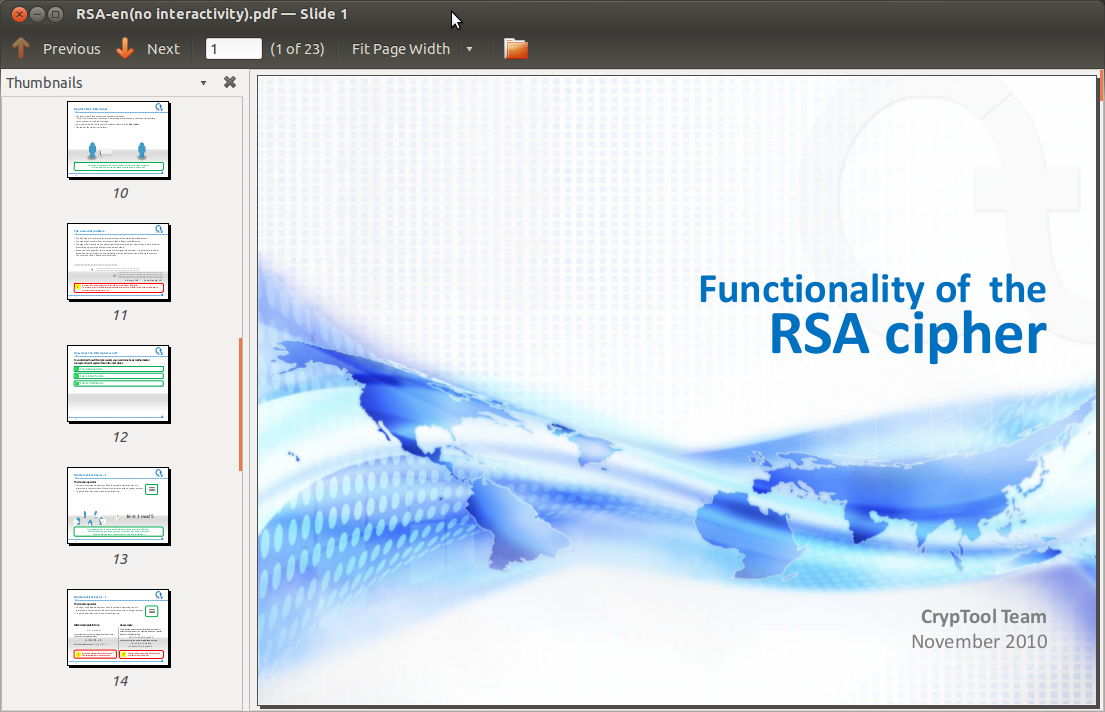
\includegraphics[scale=0.4]{figures/Interactive_RSA_Presentation_E.png}
\caption{Screenshot RSA Presentation (PDF)} 
\label{l_Interactive_RSA_Presentation}
\end{center}
\end{figure}



% ++++++++++++++++++++++++++++++++++++++++++++++++++++++++++++++++++++++++++
\newpage
\hypertarget{NumberTheory_Appendix_E}{}
\section{Appendix: Examples using Sage}
\label{NumberTheory_Appendix_E}{}
\index{Sage}
\index{Sage!Code examples}

\begin{ctsquote}
``She would never be able to tell her parents ... about any of this. She couldn't tell them about her code-breaking work. About her near death at the hands of the Daemon. About the shadowy entities pulling the strings of her government.''
\caption[Daniel Suarez]{Daniel Suarez\footnotemark}\index{Suarez, Daniel}
\end{ctsquote}
\addtocounter{footnote}{0}\footnotetext{Daniel Suarez, ``Freedom'',
  Dutton Adult, 2010, Chapter 19, ``Crossroad'', p. 229, Philips.}


\noindent Below you can find Sage source code related to contents of the
chapter~\ref{Chapter_ElementaryNT} (``\nameref{Chapter_ElementaryNT}''). 


% ---------------------------------------------------------------------------
\hypertarget{nt:AppArith1}{}
\subsection{Multiplication table modulo m}     % $ removed at $m$
\label{nt:AppArith1}{}

The multiplication table~\ref{mulmod17} (from page \pageref{SrcArith1a})
for $a \times i \pmod{m}$, where
$m = 17$, $a=5$ and $a=6$, and $i$ ranges over all integers from $0$ to $16$
can be computed using Sage as follows:

\begin{sagecode}
\begin{Verbatim}%
[fontsize=\footnotesize,fontshape=tt]
sage: m = 17; a = 5; b = 6
sage: [mod(a * i, m).lift() for i in xrange(m)]
[0, 5, 10, 15, 3, 8, 13, 1, 6, 11, 16, 4, 9, 14, 2, 7, 12]
sage: [mod(b * i, m).lift() for i in xrange(m)]
[0, 6, 12, 1, 7, 13, 2, 8, 14, 3, 9, 15, 4, 10, 16, 5, 11]
\end{Verbatim}
\caption{Multiplication tables for $a \times i \pmod{m}$ with $m = 17$, $a=5$ and $a=6$}
\end{sagecode}

\noindent The function \verb!mod()! returns an object that represents
integers modulo $m$ (in our case $m = 17$).
From the {\tt Mod} object you can get its single components either with the function
\texttt{component} or with the function \texttt{lift}.
We use the method \verb!lift()! to convert that object to an integer representation.

The other multiplication table examples modulo $13$ (table~\ref{mulmod13})
and modulo $12$ (table~\ref{mulmod12}) on page
\pageref{SrcArith1b} can similarly be computed by replacing {\tt m = 17}
with {\tt m = 13} and {\tt m = 12} respectively.


% ---------------------------------------------------------------------------
\vskip +25 pt
\hypertarget{nt:AppArith2}{}
\subsection{Fast exponentiation}
\label{nt:AppArith2}{}

The fast exponentiation modulo $m$ can be computed using the Sage
function \verb!power_mod()!. The result of this function is an
integer. We can compute the exponentiation in the example in chapter
``\nameref{hohpot}'' on page \pageref{SrcArith2} as follows:

\begin{sagecode}
\begin{Verbatim}%
[fontsize=\footnotesize,fontshape=tt]
sage: a = 87; m = 103
sage: exp = [2, 4, 8, 16, 32, 43]
sage: [power_mod(a, e, m) for e in exp]
[50, 28, 63, 55, 38, 85]
\end{Verbatim}
\caption{Fast exponentiation mod $m = 103$}
\end{sagecode}


% ---------------------------------------------------------------------------
\newpage
\hypertarget{nt:AppArith3a1}{}
\subsection{Multiplicative order}
\label{nt:AppArith3a1}{}

\noindent The order $\text{ord}_m(a)$ of a number $a$ in the multiplicative
group $\mathbf{Z}_m^{\ast}$ is the smallest number $i \geq 1$ such that
$a^i \equiv 1 \pmod{m}$ holds
(see chapter~\ref{MultOrdPrimitveRoot}, ``\nameref{MultOrdPrimitveRoot}'').
To create table~\ref{expmod11} on page~\pageref{SrcArith3a} we can print
all exponentiation $a^i \pmod{11}$ as follows:

\begin{sagecode}
\begin{Verbatim}%
[fontsize=\footnotesize,fontshape=tt]
sage: m = 11
sage: for a in xrange(1, m):
....:     print [power_mod(a, i, m) for i in xrange(1, m)]
....:
[1, 1, 1, 1, 1, 1, 1, 1, 1, 1]
[2, 4, 8, 5, 10, 9, 7, 3, 6, 1]
[3, 9, 5, 4, 1, 3, 9, 5, 4, 1]
[4, 5, 9, 3, 1, 4, 5, 9, 3, 1]
[5, 3, 4, 9, 1, 5, 3, 4, 9, 1]
[6, 3, 7, 9, 10, 5, 8, 4, 2, 1]
[7, 5, 2, 3, 10, 4, 6, 9, 8, 1]
[8, 9, 6, 4, 10, 3, 2, 5, 7, 1]
[9, 4, 3, 5, 1, 9, 4, 3, 5, 1]
[10, 1, 10, 1, 10, 1, 10, 1, 10, 1]

and including the last column with the order of each a mod (11)

sage: m = 11
sage: for a in xrange(1, m):
....:     lst= [power_mod(a, i, m) for i in xrange(1, m)]
....:     lst.append(multiplicative_order(mod(a,m)))
....:     print lst
....:
[1, 1, 1, 1, 1, 1, 1, 1, 1, 1, 1]
[2, 4, 8, 5, 10, 9, 7, 3, 6, 1, 10]
[3, 9, 5, 4, 1, 3, 9, 5, 4, 1, 5]
[4, 5, 9, 3, 1, 4, 5, 9, 3, 1, 5]
[5, 3, 4, 9, 1, 5, 3, 4, 9, 1, 5]
[6, 3, 7, 9, 10, 5, 8, 4, 2, 1, 10]
[7, 5, 2, 3, 10, 4, 6, 9, 8, 1, 10]
[8, 9, 6, 4, 10, 3, 2, 5, 7, 1, 10]
[9, 4, 3, 5, 1, 9, 4, 3, 5, 1, 5]
[10, 1, 10, 1, 10, 1, 10, 1, 10, 1, 2]
\end{Verbatim}
\caption{Table with all powers $a^i \pmod{m}$ for $m=11$, $a=1,...,10$}
\label{nt_Sage-code_MultOrder_expmod11}%Creates table with label expmod11
\end{sagecode}


\newpage
\hypertarget{nt:AppArith3b}{}
\label{nt:AppArith3b}{}

\noindent Table~\ref{expmod45} on page~\pageref{SrcArith3b} gives examples for the order modulo
45 $\text{ord}_{45}(a)$ and the Euler number $J(45)$.

\noindent The following Sage code constructs a table similar to that on page~\pageref{SrcArith3b}.

\begin{sagecode}
\begin{Verbatim}%
[fontsize=\footnotesize,fontshape=tt]
sage: m = 45
sage: for a in xrange(1, 13):
....:     lst = [power_mod(a, i, m) for i in xrange(1, 13)]
....:     try:
....:         lst.append(multiplicative_order(mod(a, m)))
....:     except:
....:         lst.append("None")
....:     lst.append(euler_phi(m))
....:     print lst
....:
[1, 1, 1, 1, 1, 1, 1, 1, 1, 1, 1, 1, 1, 24]
[2, 4, 8, 16, 32, 19, 38, 31, 17, 34, 23, 1, 12, 24]
[3, 9, 27, 36, 18, 9, 27, 36, 18, 9, 27, 36, 'None', 24]
[4, 16, 19, 31, 34, 1, 4, 16, 19, 31, 34, 1, 6, 24]
[5, 25, 35, 40, 20, 10, 5, 25, 35, 40, 20, 10, 'None', 24]
[6, 36, 36, 36, 36, 36, 36, 36, 36, 36, 36, 36, 'None', 24]
[7, 4, 28, 16, 22, 19, 43, 31, 37, 34, 13, 1, 12, 24]
[8, 19, 17, 1, 8, 19, 17, 1, 8, 19, 17, 1, 4, 24]
[9, 36, 9, 36, 9, 36, 9, 36, 9, 36, 9, 36, 'None', 24]
[10, 10, 10, 10, 10, 10, 10, 10, 10, 10, 10, 10, 'None', 24]
[11, 31, 26, 16, 41, 1, 11, 31, 26, 16, 41, 1, 6, 24]
[12, 9, 18, 36, 27, 9, 18, 36, 27, 9, 18, 36, 'None', 24]
\end{Verbatim}
\caption{Table with all powers $a^i \pmod{45}$ for $a=1,...,12$ plus the order of a}
\label{nt_Sage-code_MultOrder_expmod45}
\end{sagecode}

The number $\text{ord}_m(a)$ only exists if $a$ is relatively prime
\index{Number!co-prime} to $m$, which can be checked with \verb!gcd(a, m)!.

In the above code example, we put the calculation of the multiplicative order
within a \verb!try!-\verb!except! block. This allows Sage to catch any
exceptions or errors raised by the function \verb!multiplicative_order()!.
If an exception or error is raised in the \verb!try! block, then we know
that $\text{ord}_m(a)$ does not exist for that particular value of $a$,
hence in the \verb!except! block we append the string \verb!"None"! to
the row as represented by the object \verb!lst!.


\newpage
\hypertarget{nt:AppArith3c}{}
\label{nt:AppArith3c}{}

\noindent Table~\ref{expmod46} on page~\pageref{SrcArith3c} displays exponentiation
$a^i \pmod{46}$ as well as the order $\text{ord}_{46}(a)$.

\noindent Sage can create that table as follows:

\begin{sagecode}
\begin{Verbatim}%
[fontsize=\footnotesize,fontshape=tt]
sage: m = 46
sage: euler_phi(m)
22
sage: for a in xrange(1, 24):
....:     lst = [power_mod(a, i, m) for i in xrange(1, 24)]
....:     try:
....:         lst.append(multiplicative_order(mod(a, m)))
....:     except:
....:         lst.append("None")
....:     print lst
....:
[1, 1, 1, 1, 1, 1, 1, 1, 1, 1, 1, 1, 1, 1, 1, 1, 1, 1, 1, 1, 1, 1, 1, 1]
[2, 4, 8, 16, 32, 18, 36, 26, 6, 12, 24, 2, 4, 8, 16, 32, 18, 36, 26, 6, 12, 24, 2, 'None']
[3, 9, 27, 35, 13, 39, 25, 29, 41, 31, 1, 3, 9, 27, 35, 13, 39, 25, 29, 41, 31, 1, 3, 11]
[4, 16, 18, 26, 12, 2, 8, 32, 36, 6, 24, 4, 16, 18, 26, 12, 2, 8, 32, 36, 6, 24, 4, 'None']
[5, 25, 33, 27, 43, 31, 17, 39, 11, 9, 45, 41, 21, 13, 19, 3, 15, 29, 7, 35, 37, 1, 5, 22]
[6, 36, 32, 8, 2, 12, 26, 18, 16, 4, 24, 6, 36, 32, 8, 2, 12, 26, 18, 16, 4, 24, 6, 'None']
[7, 3, 21, 9, 17, 27, 5, 35, 15, 13, 45, 39, 43, 25, 37, 29, 19, 41, 11, 31, 33, 1, 7, 22]
[8, 18, 6, 2, 16, 36, 12, 4, 32, 26, 24, 8, 18, 6, 2, 16, 36, 12, 4, 32, 26, 24, 8, 'None']
[9, 35, 39, 29, 31, 3, 27, 13, 25, 41, 1, 9, 35, 39, 29, 31, 3, 27, 13, 25, 41, 1, 9, 11]
[10, 8, 34, 18, 42, 6, 14, 2, 20, 16, 22, 36, 38, 12, 28, 4, 40, 32, 44, 26, 30, 24, 10, 'None']
[11, 29, 43, 13, 5, 9, 7, 31, 19, 25, 45, 35, 17, 3, 33, 41, 37, 39, 15, 27, 21, 1, 11, 22]
[12, 6, 26, 36, 18, 32, 16, 8, 4, 2, 24, 12, 6, 26, 36, 18, 32, 16, 8, 4, 2, 24, 12, 'None']
[13, 31, 35, 41, 27, 29, 9, 25, 3, 39, 1, 13, 31, 35, 41, 27, 29, 9, 25, 3, 39, 1, 13, 11]
[14, 12, 30, 6, 38, 26, 42, 36, 44, 18, 22, 32, 34, 16, 40, 8, 20, 4, 10, 2, 28, 24, 14, 'None']
[15, 41, 17, 25, 7, 13, 11, 27, 37, 3, 45, 31, 5, 29, 21, 39, 33, 35, 19, 9, 43, 1, 15, 22]
[16, 26, 2, 32, 6, 4, 18, 12, 8, 36, 24, 16, 26, 2, 32, 6, 4, 18, 12, 8, 36, 24, 16, 'None']
[17, 13, 37, 31, 21, 35, 43, 41, 7, 27, 45, 29, 33, 9, 15, 25, 11, 3, 5, 39, 19, 1, 17, 22]
[18, 2, 36, 4, 26, 8, 6, 16, 12, 32, 24, 18, 2, 36, 4, 26, 8, 6, 16, 12, 32, 24, 18, 'None']
[19, 39, 5, 3, 11, 25, 15, 9, 33, 29, 45, 27, 7, 41, 43, 35, 21, 31, 37, 13, 17, 1, 19, 22]
[20, 32, 42, 12, 10, 16, 44, 6, 28, 8, 22, 26, 14, 4, 34, 36, 30, 2, 40, 18, 38, 24, 20, 'None']
[21, 27, 15, 39, 37, 41, 33, 3, 17, 35, 45, 25, 19, 31, 7, 9, 5, 13, 43, 29, 11, 1, 21, 22]
[22, 24, 22, 24, 22, 24, 22, 24, 22, 24, 22, 24, 22, 24, 22, 24, 22, 24, 22, 24, 22, 24, 22, 'None']
[23, 23, 23, 23, 23, 23, 23, 23, 23, 23, 23, 23, 23, 23, 23, 23, 23, 23, 23, 23, 23, 23, 23, 'None']
\end{Verbatim}
\caption{Table with all powers $a^i \pmod{46}$ for $a=1,...,23$ plus the order of a}
\label{nt_Sage-code_MultOrder_expmod46}
\end{sagecode}



\newpage
\hypertarget{nt:AppArith3d}{}
\label{nt:AppArith3d}{}
The following code for generating the tables~\ref{expmod14} and~\ref{expmod22}
at page~\pageref{expmod14} f. also delivers the result in a way, that in can be
easily processed in LaTeX. The prerequisite is that all content is assigned to
one Sage object (here a matrix).\footnote{%
        Remark about the Sage program, especially the Sage
        indices\index{Sage}\index{Sage!latex()}:
        \begin{compactitem}
         \item for x in xrange(2, 5) delivers 2,3,4.
         \item m = matrix(ZZ, 2, 5) has 2 rows and 5 columns.\\
               The cells are named m(0,0) to m(1,4).
         \item All elements of the matrix have to be numerical,
               so ``0'' instead of ``None'' as in the tables before.
         \item The output of matrices can be controlled in Sage with:
\begin{Verbatim}
               sage: from sage.matrix.matrix0 import set_max_cols, set_max_rows
               sage: set_max_cols(100)
               sage: set_max_rows(100)
\end{Verbatim}
         \item The length of the cycle in the last column of the tables~\ref{expmod14}
               and~\ref{expmod22} was added manually.
        \end{compactitem}
        \vspace{-\baselineskip} % Here its necessary, so that all fit to one page!
        }

\begin{sagecode}
\begin{Verbatim}%
[fontsize=\footnotesize,fontshape=tt]
def power_mod_order_matrix(m, max_a, max_i):
    r = matrix(ZZ, max_a+1, max_i+3)
    for a in xrange(0, max_a+1):
        r[a, 0] = a
        for i in xrange(1, max_i+1):
            if a==0:
                r[a,i] = i
            else:
                r[a, i] = power_mod(a, i, m)
        try:
            r[a, max_i+1] = multiplicative_order(mod(a, m))
        except:
            r[a, max_i+1] = 0
        r[a, max_i+2] = euler_phi(m)
    return r

print "\n1: m=45;max_i=13;max_a=13";m=45;max_i=13;max_a=13
r = power_mod_order_matrix(m, max_a, max_i);print r;print latex(r)

print "\n2: m=46;max_i=25;max_a=25";m=46;max_i=25;max_a=25
r = power_mod_order_matrix(m, max_a, max_i);print r.str();print latex(r)

print "\n3: m=14;max_i=13;max_a=16";m=14;max_i=13;max_a=16
r = power_mod_order_matrix(m, max_a, max_i);print r;print latex(r)

print "\n4: m=22;max_i=21;max_a=25";m=22;max_i=21;max_a=25
r = power_mod_order_matrix(m, max_a, max_i);print r.str();print latex(r)
...
3: m=14;max_i=13;max_a=16
[ 0  1  2  3  4  5  6  7  8  9 10 11 12 13  0  6]
[ 1  1  1  1  1  1  1  1  1  1  1  1  1  1  1  6]
[ 2  2  4  8  2  4  8  2  4  8  2  4  8  2  0  6]
[ 3  3  9 13 11  5  1  3  9 13 11  5  1  3  6  6]
...
\left(\begin{array}{rrrrrrrrrrrrrrrr}
0 & 1 & 2 & 3 & 4 & 5 & 6 & 7 & 8 & 9 & 10 & 11 & 12 & 13 & 0 & 6 \\
1 & 1 & 1 & 1 & 1 & 1 & 1 & 1 & 1 & 1 & 1 & 1 & 1 & 1 & 1 & 6 \\
2 & 2 & 4 & 8 & 2 & 4 & 8 & 2 & 4 & 8 & 2 & 4 & 8 & 2 & 0 & 6 \\
3 & 3 & 9 & 13 & 11 & 5 & 1 & 3 & 9 & 13 & 11 & 5 & 1 & 3 & 6 & 6 \\
...
\end{Verbatim}
\caption{Code for tables with all powers $a^i \pmod{m}$ for variable $a$ and $i$ plus order of a and Eulerphi of m}
\end{sagecode}




% ---------------------------------------------------------------------------
\newpage
\hypertarget{nt:AppArith3a2}{}
\subsection{Primitive roots}
\label{nt:AppArith3a2}
\label{primitive-roots-with-sage}
\index{Primitive root}

Computing a primitive root (see chapter~\ref{MultOrdPrimitveRoot},
``\nameref{MultOrdPrimitveRoot}'')
in Sage is very straightforward. If \verb!n! is an integer, the command
\verb!primitive_root(n)! computes \textit{one} primitive root of the multiplicative group
$(\mathbf{Z} / n \mathbf{Z})^{\ast}$, if one exists.
Where $n$ is prime, then this is the same as calculating a primitive root of
$\mathbf{Z} / n \mathbf{Z}$.

\noindent Here, we calculate some primitive roots of a few integers.

\begin{sagecode}
\begin{Verbatim}%
[fontsize=\footnotesize,fontshape=tt]
sage: primitive_root(4)
3
sage: primitive_root(22)
13
sage: for p in primes(1, 50):
....:     print p, primitive_root(p)
....:     
2 1
3 2
5 2
7 3
11 2
13 2
17 3
19 2
23 5
29 2
31 3
37 2
41 6
43 3
47 5
\end{Verbatim}
\caption{Calculating one primitive root for a given prime}
\end{sagecode}

\noindent If $p$ is prime, then $\mathbf{Z} / p \mathbf{Z}$ has at least one
primitive root.



\newpage
\noindent Sometimes we want to compute \texttt{all} the primitive roots
of $\mathbf{Z} / p \mathbf{Z}$, not just any primitive root of
$\mathbf{Z} / p \mathbf{Z}$.
The following function can do this%
\footnote{This code was developed in a Sage script file and
executed non-interactively. That is why you don't see "sage:" and "....:"
at the beginning of the lines like in the Sage samples before.}.

\begin{sagecode}
\begin{Verbatim}%
[fontsize=\footnotesize,fontshape=tt]
def enum_PrimitiveRoots_of_an_Integer(M):
    r"""
    Return all the primitive roots of the integer M (if possible).
    """
    try:
        g = primitive_root(M)
    except:
        return None
    targetOrder = euler_phi(M)
    L=[]
    # Stepping through all odd integers from 1 up to M, not including
    # M. So this loop only considers values of i where 1 <= i < M.
    for i in xrange(1,M,2):
            testGen = Mod(g^i,M)
            if testGen.multiplicative_order() == targetOrder:
                L.append(testGen.lift())
    # removing duplicates
    return Set(L)

# AA_Start -- Testcases for enum_PrimitiveRoots_of_an_Integer(M)
print "AA_Start -- Testcases for enum_PrimitiveRoots_of_an_Integer(M)"
M=10; print "1-----------Testcase: M = %s" % M
LL = enum_PrimitiveRoots_of_an_Integer(M)
if LL==None:
    print M
else:
    print LL
M=8; print "2-----------Testcase: M = %s" % M
# M=8 hat keine primitive root mod m. Checke, ob per try - except abgefangen.
LL = enum_PrimitiveRoots_of_an_Integer(M)
if LL==None:
    print M
else:
    print LL
M=17; print "3-----------Testcase: M = %s" % M
LL = enum_PrimitiveRoots_of_an_Integer(M)
if LL==None:
    print M
else:
    print LL
# AA_End -- Testcases

OUTPUT:
AA_Start -- Testcases for enum_PrimitiveRoots_of_an_Integer(M)
1-----------Testcase: M = 10
{3, 7}
2-----------Testcase: M = 8
8
3-----------Testcase: M = 17
{3, 5, 6, 7, 10, 11, 12, 14}
\end{Verbatim}
\caption{Function ``enum\_PrimitiveRoots\_of\_an\_Integer'' to calculate all primitive
roots for a given number}
\end{sagecode}



\newpage
\noindent For example, here is a list of all primitive roots of the prime 541.

\begin{sagecode}
\begin{Verbatim}%
[fontsize=\footnotesize,fontshape=tt]
sage: L=enum_PrimitiveRoots_of_an_Integer(541); L
{2, 517, 10, 523, 13, 14, 527, 528, 18, 531, 24, 539, 30, 37, 40, 51,
54, 55, 59, 62, 65, 67, 68, 72, 73, 77, 83, 86, 87, 91, 94, 96, 98,
99, 107, 113, 114, 116, 117, 126, 127, 128, 131, 132, 138, 150, 152,
153, 156, 158, 163, 176, 181, 183, 184, 195, 197, 199, 206, 208,
210, 213, 218, 220, 223, 224, 244, 248, 250, 257, 258, 259, 260,
261, 263, 267, 269, 270, 271, 272, 274, 278, 280, 281, 282, 283,
284, 291, 293, 297, 317, 318, 321, 323, 328, 331, 333, 335, 342,
344, 346, 357, 358, 360, 365, 378, 383, 385, 388, 389, 391, 403,
409, 410, 413, 414, 415, 424, 425, 427, 428, 434, 442, 443, 445,
447, 450, 454, 455, 458, 464, 468, 469, 473, 474, 476, 479, 482,
486, 487, 490, 501, 504, 511}
sage: len(L)
144
\end{Verbatim}
\caption{Table with all primitive roots for the given prime 541}
\end{sagecode}



\newpage
\noindent With a little bit of programming, we can count how many primitive roots
are in a given range of integers. We can check this for all numbers or only for the
primes within this range.

\begin{sagecode}
\begin{Verbatim}%
[fontsize=\footnotesize,fontshape=tt]
def count_PrimitiveRoots_of_an_IntegerRange(start, end, bPrimesOnly=True):
	r"""
	Compute all primitive roots of all numbers between start and end,
	inclusive, and count them.
	If the flag bPrimesOnly is True, it performs primality tests, so it
	allows us to count the number of primes from start to end, inclusive.
        If the flag bPrimesOnly is false, it additionally counts these even
	numbers which have no primitive root.
	"""
	nCheckedNumb = 0
	nCheckedNumb_WithoutPrimitivRoots = 0
	nPrimitiveRoots = 0
	for n in xrange(start, end+1):
		if bPrimesOnly:
			if is_prime(n):
				nCheckedNumb += 1
				L = enum_PrimitiveRoots_of_an_Integer(n)
				nPrimitiveRoots += len(L)
		else:
			nCheckedNumb += 1
			L = enum_PrimitiveRoots_of_an_Integer(n)
			if L==None:
				nCheckedNumb_WithoutPrimitivRoots += 1
			else:
				nPrimitiveRoots += len(L)

	if bPrimesOnly:
		print "Found all %s" % nPrimitiveRoots + \
		      " primitive roots of %s primes." % nCheckedNumb
	else:
		if nCheckedNumb_WithoutPrimitivRoots == 0:
			print "Found all %s " % nPrimitiveRoots + \
			      "primitive roots of %s numbers." % nCheckedNumb
		else:
			print "Found all %s " % nPrimitiveRoots + \
			      "primitive roots of %s numbers." % \
			          (nCheckedNumb - nCheckedNumb_WithoutPrimitivRoots)
			print "(Total of numbers checked: %s, " % nCheckedNumb + \
			      "Amount of numbers without primitive roots: %s)" % \
			          nCheckedNumb_WithoutPrimitivRoots
\end{Verbatim}
\caption{Function ``count\_PrimitiveRoots\_of\_an\_IntegerRange'' to calculate all
primitive roots for a given range of integers}
\end{sagecode}


\newpage
\noindent Using the Sage command \verb!time!, we can also find out how long it takes on
our computer.

\begin{sagecode}
\begin{Verbatim}%
[fontsize=\footnotesize,fontshape=tt]
# BB_Start -- Testcases for count_PrimitiveRoots_of_an_IntegerRange(start, end, bPrimesOnly=True)
print "\n\nBB_Start -- Testcases for count_PrimitiveRoots_of_an_IntegerRange(start, end, True)"

print "\n1-----------Testcase: (1, 500)"
time count_PrimitiveRoots_of_an_IntegerRange(1, 500)

print "\n2-----------Testcase: (5, 6, False)"
time count_PrimitiveRoots_of_an_IntegerRange(5, 6, False)

print "\n3-----------Testcase: (1, 500, False)"
time count_PrimitiveRoots_of_an_IntegerRange(1, 500, False)
# BB_End -- Testcases

OUTPUT:
BB_Start -- Testcases for count_PrimitiveRoots_of_an_IntegerRange(start, end, bPrimesOnly=True)

1-----------Testcase: (1, 500)
Found all 8070 primitive roots of 95 primes.
Time: CPU 0.94 s, Wall: 0.97 s

2-----------Testcase: (5, 6, False)
Found all 3 primitive roots of 2 numbers.
Time: CPU 0.00 s, Wall: 0.00 s

3-----------Testcase: (1, 500, False)
Found all 11010 primitive roots of 170 numbers.
(Total of numbers checked: 500, Amount of numbers without primitive roots: 330)
Time: CPU 1.52 s, Wall: 1.59 s
\end{Verbatim}
\caption{Function ``count\_PrimitiveRoots\_of\_an\_IntegerRange'': testcases and output}
\end{sagecode}




\newpage
\noindent Using our custom-defined function \verb!enum_PrimitiveRoots_of_an_Integer!,
we can find all primitive roots of one prime integer $p$.

The following function counts how many primes are in a given range
and enumerate all their primitive roots.

From this list of primitive roots, we can determine the smallest and largest
primitive root for $\mathbf{Z} / p \mathbf{Z}$, as well as count the number
of primitive roots of $\mathbf{Z} / p \mathbf{Z}$.

\begin{sagecode}
\begin{Verbatim}%
[fontsize=\footnotesize,fontshape=tt]
def count_PrimitiveRoots_of_a_PrimesRange(start, end):
      r"""
      Compute all primitive roots of all primes between start and end,
      inclusive. This uses a primes iterator.
      """
      nPrimes = 0
      nPrimitiveRoots = 0
      for p in primes(start, end+1):
          L = enum_PrimitiveRoots_of_an_Integer(p)
	  print p, len(L)
          nPrimes += 1
          nPrimitiveRoots += len(L)
      print "Found all %s" % nPrimitiveRoots + " primitive roots of %s primes." % nPrimes

# CC_Start -- Testcases for count_PrimitiveRoots_of_a_PrimesRange(start, end)
print "\n\nBB_Start -- Testcases for count_PrimitiveRoots_of_a_PrimesRange(start, end)"
print "-----------Testcase: (1, 1500)"
time count_PrimitiveRoots_of_a_PrimesRange(1, 1500)
# CC_End -- Testcases

OUTPUT:
CC_Start -- Testcases for count_PrimitiveRoots_of_a_PrimesRange(start, end)
-----------Testcase: (1, 1500)
2 1
3 1
5 2
7 2
11 4
13 4
17 8
19 6
23 10
29 12
31 8
37 12
...
1483 432
1487 742
1489 480
1493 744
1499 636
Found all 62044 primitive roots of 239 primes.
Time: CPU 7.55 s, Wall: 7.85 s
\end{Verbatim}
\caption{Function ``count\_PrimitiveRoots\_of\_a\_PrimesRange'' to calculate the number
of primitive roots for a given range of primes}
\end{sagecode}



\newpage
\noindent A slightly modified version of our function
\verb!count_PrimitiveRoots_of_a_PrimesRange!, was used to generate
a database of all primitive roots of all primes between 1 and 100,000.

\begin{sagecode}
\begin{Verbatim}%
[fontsize=\footnotesize,fontshape=tt]
start = 1
end = 10^5
fileName = "/scratch/mvngu/primroots.dat"
file = open(fileName, "w")
for p in primes(start, end+1):
    L = enum_PrimitiveRoots_of_an_Integer(p)
    print p, len(L)
    # Output to a file. The format is:
    # (1) the prime number p under consideration
    # (2) the number of primitive roots of Z/pZ
    # (3) all the primitive roots of Z/pZ
    file.write(str(p) + " " + str(len(L)) + " " + str(L) + "\n")
    file.flush()
file.close()
\end{Verbatim}
\caption{Code to generate the database with all primitive roots for all primes between
1 and 100,000}
\end{sagecode}

It took about one day on the machine sage.math to generate the
file ``primroots.dat'' (done in July 2009 by Minh Van Nguyen).

This code and the function \verb!enum_PrimitiveRoots_of_an_Integer!
was put in a Sage script file and executed non-interactively.

The file ``primroots.dat'' is a database of all primitive roots of all primes
between 1 and 100,000 inclusive. It is a very large file (about 1 GB
uncompressed, and 285 MB compressed with bzip2). You can find the file
at {\url{http://sage.math.washington.edu/home/mvngu/doc/primitive-roots/primroots.dat.bz2}}.



\newpage
\noindent This database file ``primroots.dat'' was used then to create three graphics using the following code.

\begin{sagecode}
\begin{Verbatim}%
[fontsize=\footnotesize,fontshape=tt]
sage: # open a database file on primitive roots from 1 to 100,000
sage: file = open("/scratch/mvngu/primroots.dat", "r")
sage: plist = []    # list of all primes from 1 to 100,000
sage: nlist = []    # number of primitive roots modulo prime p
sage: minlist = []  # smallest primitive root modulo prime p
sage: maxlist = []  # largest primitive root modulo prime p
sage: for line in file:
....:     # get a line from the database file and tokenize it for processing
....:     line = line.strip().split(" ", 2)
....:     # extract the prime number p in question
....:     plist.append(Integer(line[0]))
....:     # extract the number of primitive roots modulo p
....:     nlist.append(Integer(line[1]))
....:     # extract the list of all primitive roots modulo p
....:     line = line[-1]
....:     line = line.replace("{", "")
....:     line = line.replace("}", "")
....:     line = line.split(", ")
....:     # sort the list in non-decreasing order
....:     line = [Integer(s) for s in line]
....:     line.sort()
....:     # get the smallest primitive root modulo p
....:     minlist.append(line[0])
....:     # get the largest primitive root modulo p
....:     maxlist.append(line[-1])
....:
sage: file.close()  # close the database file
sage: # plot of number of primitive roots modulo p
sage: nplot = point2d(zip(plist, nlist), pointsize=1)
sage: nplot.axes_labels(["x", "y"])
sage: nplot
sage: # plot of smallest primitive root modulo prime p
sage: minplot = point2d(zip(plist, minlist), pointsize=1)
sage: minplot.axes_labels(["x", "y"])
sage: minplot
sage: # plot of largest primitive root modulo prime p
sage: maxplot = point2d(zip(plist, maxlist), pointsize=1)
sage: maxplot.axes_labels(["x", "y"])
sage: maxplot
\end{Verbatim}
\caption{Code to generate the graphics about the primitive roots}
\end{sagecode}




\newpage
Figure~\ref{fig:primitive_roots_all} graphs the number of primitive
roots for each prime between 1 and 100,000. The $x$-axis represents
primes between 1 and 100,000, while the $y$-axis counts the number of
primitive roots for each prime within that interval.

\begin{figure}[!htbp]
\centering
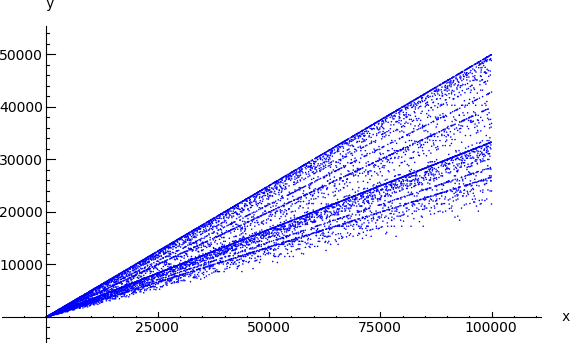
\includegraphics{figures/primitive-roots-all}
\caption{The number of primitive roots of all primes between 1 and 100,000.}
\label{fig:primitive_roots_all}
\end{figure}

\vskip +50 pt
Figure~\ref{fig:primitive_roots_smallest} graphs the smallest
primitive roots of all primes between 1 and 100,000. The $x$-axis
represents primes between 1 and 100,000. The $y$-axis represents the
smallest primitive root of each prime within that
interval.

\vskip +25 pt
Figure~\ref{fig:primitive_roots_largest} shows a
corresponding graph for the largest primitive root of each prime
within the above interval.

\begin{figure}[!htbp]
\centering
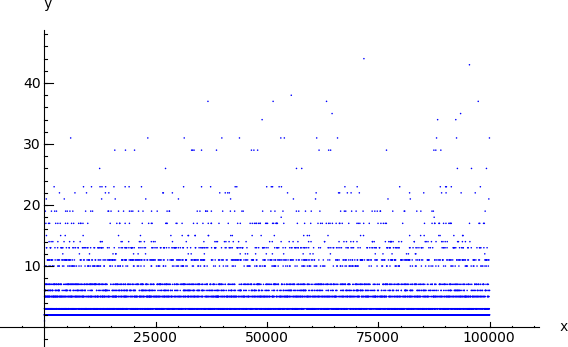
\includegraphics{figures/primitive-roots-smallest}
\caption{The smallest primitive roots of all primes between 1 and 100,000.}
\label{fig:primitive_roots_smallest}
\end{figure}

\begin{figure}[!htbp]
\centering
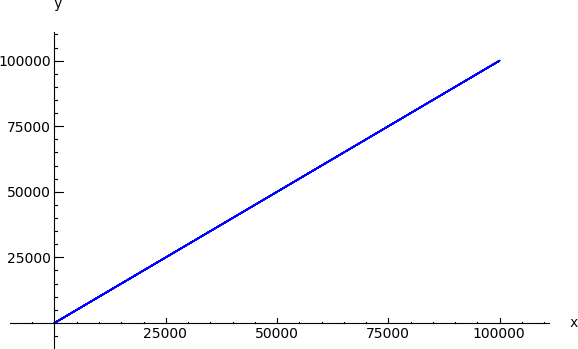
\includegraphics{figures/primitive-roots-largest}
\caption{The largest primitive roots of all primes between 1 and 100,000.}
\label{fig:primitive_roots_largest}
\end{figure}




% ---------------------------------------------------------------------------
\newpage
\hypertarget{NumberTheory_Sage_RSA sample}{}
\subsection{RSA examples with Sage}
\label{l:NumberTheory_Sage_RSA sample}{}

\noindent Below is Sage source code for the simple RSA examples in
section~\ref{rsaconcrete} (``\nameref{rsaconcrete}''). 

\vskip +10 pt 
\hypertarget{nt:AppArith4a}{%
\noindent \textbf{Example on page~\pageref{SrcArith4a}:}}
\label{nt:AppArith4a}\\
The RSA exponentiation $M^{37} \pmod{3713}$ on message $M = 120$ can be
calculated in Sage as follows:

\begin{Verbatim}%
[fontsize=\footnotesize,fontshape=tt]
sage: power_mod(120, 37, 3713)
1404
\end{Verbatim}


\vskip +10 pt 
\hypertarget{nt:AppArith4b}{%
\noindent {\bf Example on page~\pageref{SrcArith4b}:}}
\label{nt:AppArith4b}\\
The factorization of $J(256027) = 255016 = 2^3 * 127 * 251$ can be
calculated using Sage as follows:

\begin{sagecode}
\begin{Verbatim}%
[fontsize=\footnotesize,fontshape=tt]
sage: factor(255016)
2^3 * 127 * 251
\end{Verbatim}
\caption{Factoring a number}
\end{sagecode}


\vskip +10 pt 
\hypertarget{nt:AppArith4c}{%
\noindent {\bf Example on page~\pageref{SrcArith4c}:}}
\label{nt:AppArith4c}\\
Sage can do RSA encryption as follows:

\begin{sagecode}
\begin{Verbatim}%
[fontsize=\footnotesize,fontshape=tt]
sage: A = [82, 83, 65, 32, 119, 111, 114, 107, 115, 33]
sage: e = 65537; m = 256027
sage: [power_mod(a, e, m) for a in A]
[212984, 25546, 104529, 31692, 248407, 100412, 54196, 100184, 58179, 227433]
\end{Verbatim}
\caption{RSA encryption by modular exponentiation of a number (used as message)}
\end{sagecode}


\vskip +10 pt 
\hypertarget{nt:AppArith4d}{%
\noindent {\bf Example on page~\pageref{SrcArith4d}:}}
\label{nt:AppArith4d}\\
RSA encryption using Sage:

\begin{Verbatim}%
[fontsize=\footnotesize,fontshape=tt]
sage: A = [21075, 16672, 30575, 29291, 29473]
sage: e = 65537; m = 256027
sage: [power_mod(a, e, m) for a in A]
[158721, 137346, 37358, 240130, 112898]
\end{Verbatim}


\vskip +10 pt 
\hypertarget{nt:AppArith4e}{%
\noindent {\bf Example on page~\pageref{SrcArith4e}:}}
\label{nt:AppArith4e}\\
RSA encryption using Sage:

\begin{Verbatim}%
[fontsize=\footnotesize,fontshape=tt]
sage: A = [82083, 65032, 119111, 114107, 115033]
sage: e = 65537; m = 256027
sage: [power_mod(a, e, m) for a in A]
[198967, 51405, 254571, 115318, 14251]
\end{Verbatim}




% ---------------------------------------------------------------------------
\newpage
\hypertarget{NumberTheory_Sage_Number-of-RSA-keys}{}
\subsection{How many private RSA keys $d$ exist within a given modulo range?}
\label{l:NumberTheory_Sage_Number-of-RSA-keys}{}

The RSA encryption procedure was described in section \ref{RSA} (``\nameref{RSA}'').
Steps 1 to 3 constitute key generation, steps 4 and 5 are the encryption:
\begin{itemize}
  \item[{\bf 1.}] Select two distinct random prime numbers $p$ and $q$
                  and calculate $n = p*q$.\\
                  The value $n$ is called the RSA modulus.

  \item[{\bf 2.}] Select an arbitrary $e \in \{2, \cdots, n-1\}$ such that: \\
                  $e$ is relatively prime
                  \index{Prime number!relative prime}\index{Number!relative prime}
                  to $J(n) = (p-1)*(q-1)$. \\
                  We can then ``throw away'' $p$ and $q$.

  \item[{\bf 3.}] Select $d \in \{1, \cdots, n-1\}$ with $e*d \equiv 1  
                  {\rm ~(mod~} J(n))$,\\
		  i.e. $d$ is the multiplicative inverse of $e$ modulo $J(n)$.
		  We can then ``throw away'' $J(n)$.
    \begin{compactitem}
        \item[] $\rightarrow (n, e)$ is the public key $P$.
        \item[] $\rightarrow (n, d)$ is the private key $S$ (only $d$ must be kept secret).
    \end{compactitem}

  \item[{\bf 4.}] For encryption, the message represented as a (binary) number
                  is divided into parts such that each part of 
                  the number represents a number less than $n$.

  \item[{\bf 5.}] Encryption of the plaintext (or the parts of it) $M \in \{1, \cdots, n-1\}$:
                  $$C = E ( (n, e); M ) := M^e {\rm ~(mod~} n).$$
\end{itemize}

The default way to crack a given RSA ciphertext $C$ would be to use the public key
of the recipient and to try to factorize $n$. Then you can go through the steps 2 and 3
and generate the private key $e$, which is normally used to decrypt a ciphertext.

According to the ``prime number theorem''\footnote{%
See section \ref{thm-pz-pi-x} (``\nameref{l_Primes_Distrib-of-Primes}'').
}
the number of prime numbers $PI(x)$ is asymptotic to  $x / ln(x)$.
%% So in a given range $[x,y]$ there are about $ (y / ln(y)) - (x / ln(x))$ primes.
Between $1$ and a given $n$ there are about $n / ln(n)$ different primes.
%% (not considering the more specific requirements for selecting
%%  appropriate values for $p$ as described above).

\noindent If you don't want to use factorization but ask the question like in classic
encryption, you may want to find out:
How many possible private keys $(n, d)$ are there for a given key size range
$n \in [a, b]$?\footnote{%
Chapter~\ref{L_nt_Num-of-d-mod-26} (``\nameref{L_nt_Num-of-d-mod-26}''),
p.~\pageref{L_nt_Num-of-d-mod-26} deals with the special case $n=26$.}
%% (this means, only a part of each public key $(n, e)$ is known).

\noindent Sage source code~\ref{nt_sagesample_Count_RSA_Keys} below defining the
function \verb#count_Number_of_RSA_Keys# can answer this question concretely
(if the modulus is not too big).\footnote{%
%\begin{compactitem}
\newlength{\saveleftmargini}
\setlength{\saveleftmargini}{\leftmargini}
\setlength{\leftmargini}{0em}% for example to outdent verse
\settowidth{\versewidth}{xxxxx xxxxx xxxxx xxxxx xxxxx xxxxx xxxxx xxxxx xxxxx xxxxx xxxxx xxxxx xxxxx xxxxx xxxxx xxxxx xxxxx xxxxx}
\vspace{-\baselineskip} % TODO: Geht das nicht anders?
\begin{verse}[\versewidth]
 a) Calling \verb#sage: count_Number_of_RSA_Keys(100, 1000)# means to consider the interval
$[100, 1000]$ for $n$.
\verselinebreak $n$ is defined by the two primes $p, q: n = p*q$.
\verselinebreak So here one prime can have the maximal value $500$ because $2 * 500 =1000$
(while then the other prime will have the smallest possible prime value $2$).\\
\vin The number of possible combinations of primes is $comb = 258$.\\
\vin The number of primes in the given range is $143$.\\
\vin The number of private keys is $34,816$.
\end{verse}
%\noindent %       \item
\begin{verse}[\versewidth]
 b) Calling \verb#sage: count_Number_of_RSA_Keys(100, 100, True)# has the
following output:\\
\vin    - Number of private keys for modulus in a given range: 0\\
\vin    - Number of primes in a given range: 0\\
\vin    The reason for that is, that with this call only $n=100$ is considered,
   and the function investigates only\\
\vin semiprime $n$: $100$ is not semi prime\index{Prime number!semi
   prime}\index{Prime number!half prime},
   this means $100$ is not the product of only two primes.
\end{verse}
\setlength{\leftmargini}{\saveleftmargini}% restore original value%\end{compactitem}
}


\begin{sagecode}
\begin{Verbatim}%
[fontsize=\footnotesize,fontshape=tt]
def count_Number_of_RSA_Keys(start, end, Verbose=False):
      r"""
      How many private RSA keys (n,d) exist, if only modulus N is given, and start <= N <= end?
        (prime_range(u,o) delivers all primes >=u und < o).
      """
      a = start
      b = end
      s = 0
      comb = 0
      for p in prime_range(1, b/2+1):
          for q in prime_range(p + 1, b/2+1):
              if a <= p * q and p * q <= b:
                  comb = comb +1
                  s = s + (euler_phi(euler_phi(p * q))-1)
                  if Verbose:
                      print "p=%s, " % p + "q=%s, " % q + "s=%s" % s
      print "Number of private keys d for modulus in a given range: %s" % s + " (comb=%s), " % comb

      # Just for comparison: How many primes are in this range?
      s = 0
      for p in prime_range(a, b+1):
          if Verbose:
              print "a=%s, " % a + "b=%s, " % b + "p=%s" % p
          s = s + 1
      print "Number of primes in a given range: %s" % s

print "\n\nDD_Start -- Testcases for count_Number_of_RSA_Keys(start, end)"
print "\n-----------Testcase: (100, 1000) [Should deliver 34.816]"
time count_Number_of_RSA_Keys(100, 1000)
print "\n-----------Testcase: (100, 107, True) [Should deliver 23]"
time count_Number_of_RSA_Keys(100, 107, True)
u = 10^3; o = 10^4;
print "\n-----------Testcase: (%s, " % u + "%s) [Should deliver 3.260.044]" % o
time count_Number_of_RSA_Keys(u, o)

OUTPUT:
DD_Start -- Testcases for count_Number_of_RSA_Keys(start, end)

-----------Testcase: (100, 1000) [Should deliver 34.816]
Number of private keys d for modulus in a given range: 34816 (comb=258),
Number of primes in a given range: 143
Time: CPU 0.03 s, Wall: 0.04 s

-----------Testcase: (100, 107, True) [Should deliver 23]
p=2, q=53, s=23
Number of private keys d for modulus in a given range: 23 (comb=1),
a=100, b=107, p=101
a=100, b=107, p=103
a=100, b=107, p=107
Number of primes in a given range: 3
Time: CPU 0.00 s, Wall: 0.00 s

-----------Testcase: (1000, 10000) [Should deliver 3,260,044]
Number of private keys d for modulus in a given range: 3260044 (comb=2312),
Number of primes in a given range: 1061
Time: CPU 0.63 s, Wall: 0.66 s
\end{Verbatim}
\caption{How many private RSA keys d are there if you know a range for the public key n?}
\label{nt_sagesample_Count_RSA_Keys}
\end{sagecode}

\noindent As there are many more private keys $(n, d)$ within a
bigger range of values for $n$, even brute-force factoring
is much more efficient as brute-force trying all the keys.




% ---------------------------------------------------------------------------
\clearpage
\newpage
\hypertarget{NumberTheory_Sage_Number-of-RSA-FixedPoints}{}
\subsection
    [RSA fixed points \texorpdfstring{}{m = m\^{}e}]
    {RSA fixed points $ m^e = m \bmod n $ mit $m \in \{1,...,n-1\}$ }
\label{l:NumberTheory_Sage_Number-of-RSA-FixedPoints}{}
\index{Fixpoint}\index{RSA!fixpoint}
%%% xxx111222xxx-beg

Also encryption methods can have fixed -- cleartext messages where the
according ciphertext matches the original. In mathematics, variables
mapped by the algorithm (function) onto themselves are called fixed points.
In cryptography the according messages are called ``unconcealed messages''.

Generally speaking: The more fixed points an encryption algorithm contains,
the easier it is to break it.

With the RSA procedure: $n=pq$ is the product of two different prime numbers,
and there exists $e$ where $gcd(e,(p-1)(q-1))=1$. The encription is then
$c = m^e \mod n$. 
A fixed point in the RSA procedure is a message $m$, where: 
$m = m^e \mod n$. 
The result of the encryption is the given message.

When the size of $n$ is sufficiently big, the probability of the occurance of
fixed points in RSA is very small -- as illustrated in Figure
\ref{fig:NumberFixpointsGrowingN}: In average, we found not more than 40 fixed
points.

Students often presume the occurence of fixed points high, because they counter
a ``relatively'' large number of examples when experimenting with \textbf{small}
prime numbers, as m = 0, 1 and n-1 are also always fixed points.

In practice, where large prime numbers are chosen, fixed points have no
significance for the security of RSA. Therefore, this paragraph refers more
to the mathematical questions.\footnote{%
Thanks to Taras Shevchenko for gathering parts of the content of this chapter
and to Volker Simon for writing the Sage program
\ref{nt_sagesample_Calculate_RSA-Fixpoints} ``Getfixpoints''.}


% ----------------------------------------------------
\subsubsection{The number of RSA fixed points}

In this section we show how many RSA fixed points there are for $m \in \{1,...,n-1\} $.\\

\begin{theorem}\label{nt-number-of-fixpoints-1-to-n-1}
The number of the fixed points $ m^e = m \bmod n$ with $m \in \{1,...,n-1\} $ is \\$ gcd(p-1, e-1) \cdot gcd(q-1, e-1) $.
\end{theorem}
\begin{proof}
Given $m^e = m \bmod n.$
According to the CRT\index{CRT}\footnote{%
CRT = Chinese Remainder Theorem.
\url{http://en.wikipedia.org/wiki/Chinese_Remainder_Theorem}
}, the following statements are equivalent:\\
$$ [ m^e = m \bmod n ]  \Leftrightarrow [ m^{e} = m \bmod p \text{  and  } m^{e} = m \bmod q ] $$
% STH: consider using 'analysis' instead of 'decomposition'
%      be: Kl�ren, denn es ist auch keine �quivalenz! xxxxxxxxxxxxxxxxxxxxxxxxxxxxxxxxx
This decomposition is equivalent to:
$$m^{e-1} = 1 \bmod p \text{  and  } m^{e-1} = 1 \bmod q. $$

\noindent We consider  $m^{e-1} = 1 \bmod p$ and search all $(e-1)$
roots of unity\index{RootOfUnity}\footnote{%
- In mathematics, a \textbf{root of unity} is a number $x$ that equals 1 when raised to some integer power $n$.

\noindent- An $n$-th root of unity $x$ is \textbf{primitive} if it is not a $k$-th root of unity for all integers $k$ smaller than $n$:
 $$x^{n} = 1  \text{ and }    x^{k} \neq 1 ~~~(k = 1,2, 3, ..., n-1)$$

\noindent-
If $F$ is a finite field and $n$ is a positive integer, then a $n$th-root of unity in $F$ is a solution of the equation $$ x^{n}-1 = 0 \text{ in } F $$
}
in $\mathbb{Z}_p^{*}.$\\
It holds: $\mathbb{Z}_p^{*}$ for p prime is cyclic.~~$\Rightarrow $~~
A generator $g$ exists which produces $\mathbb{Z}_p^{*}$: $\mathbb{Z}_p^{*}=<g>$.\\

\noindent The following theorem from \cite[Pg. 69]{nt:Katzenbeisser2001}\index{Katzenbeisser 2001} characterizes all $(e-1)$-th roots of unity in $\mathbb{Z}_p^{*}$:
\begin{theorem}\label{nt-katzenbeisser-Anzahl-Einheitswurzeln}
$g^{\alpha}$ is exactly then $(e-1)$-th root of unity in $\mathbb{Z}_p^{*}$,
when $(e-1)\alpha = 0\bmod p-1.$ There are $gcd(p-1, e-1)$ of these.
\end{theorem}
\begin{proof} 
The first thesis results directly from the small theorem from Fermat:
\[g^{\alpha (e-1)}= 1 \bmod p  ~~\Rightarrow~~ \alpha (e-1) = 0\bmod p-1 \]
Let $\delta =gcd(p-1, e-1)$.  $\alpha (e-1) = 0\bmod p-1$ implies $\frac{\alpha (e-1)}{\delta}= 0 \bmod \frac{p-1}{\delta}$. \\
Since $\frac {e-1}{\delta}$ and $\frac{p-1}{\delta}$ are coprime (each was 
reduced by the gcd of their corresponding numerator),
$\alpha$ must be a multiple of $\frac{p-1}{\delta}$.

\[ \alpha \frac{p-1}{\delta} ~~ \text{with} ~~ \alpha = 1,...,\delta
\]\\
These $\delta$ different powers then correspond to the 
$(e-1)$-th roots of unity $g^{\alpha \frac{p-1}{\delta}} \bmod p$ in $\mathbb{Z}_p^{*}$.
\end{proof}

\noindent Analog for $q$: For $m^{e-1} = 1 \bmod q $ we then have $ gcd(q-1, e-1) $ many of $(e-1)$-th roots of unity.\\

\noindent The number of combinations of the $(e-1)$-th root of unity in $\mathbb{Z}_p^{*}$ and
$\mathbb{Z}_q^{*}$ gives the total quantity of RSA fixed points:
$ m^e = m \bmod n$ with $ m \in \{1,...,n-1\}$:\\
 $gcd(p-1, e-1) \cdot gcd(q-1, e-1) $\\

\noindent Adding $m=0$ to the above, results in the theorem \ref{nt-thm-Anzahl-RSA-Fixpunkte}:
\begin{theorem}\label{nt-thm-Anzahl-RSA-Fixpunkte}
If $ m \in \{0,...,n-1\}$, then the quantity of the RSA fixed points is:
          \[ (gcd(p-1, e-1)+1) \cdot (gcd(q-1, e-1)+1) \]
\end{theorem}
\end{proof}
\vspace{15pt}



% ----------------------------------------------------
\subsubsection{Lower bound for the quantity of RSA fixed points}
In the following section, we show that there is a lower bound for the quantity of RSA fixed points. This lower bound $6$ exists when the two different RSA prime numbers are the smallest possible values (2 and 3).\\

\noindent\textbf{Thesis 1: $p = 2, q = 3$}\\
The quantity of RSA fixed points for $p=2$ and $q=3$ is\\
$(\underbrace{gcd(p-1, e-1)}_{=1}+1) \cdot (\underbrace{gcd(q-1, e-1)}_{=2}+1)=2 \cdot 3=6$ \\

\noindent\textbf{Thesis 2: $p \neq q; p > 2, q > 2$}\\
The quantity of RSA fixed points for $p \neq q; p,q > 2$ is $\geq 9$.

\begin{proof}
Since $p$ and $q$ are prime, $(p-1)$ and $(q-1)$ for $ p,q > 2 $ are even.\\
The RSA algorithm requires to choose e so that $1 < e < \phi(n)=(p-1)(q-1)$ and \\
$gcd(e,(p-1)(q-1))=1$\\
Since $(p-1)$ and $(q-1)$ are even, e is odd $ \Rightarrow e-1$ is even.\\
Since $(p-1)$ and $(e-1)$ are even, then:\\
$gcd(p-1, e-1) \geq 2$ \\
$\Rightarrow (gcd(p-1, e-1)+1) \geq 3$ and $(gcd(q-1, e-1)+1) \geq 3$\\
$\Rightarrow (gcd(p-1, e-1)+1) \cdot (gcd(q-1, e-1)+1) \geq 9$
\end{proof}

\noindent Samples:\\
For $(e,n)=(17,6)$, all six possible messages \{0,1,2,3,4,5\} are
fixed points (for $n=6$, it is independent from the value of $e$).\\
For $(e,n)=(17,10)$, all 10 possible messages are fixed points.\\
For $(e,n)=(19,10)$, only 6 of the 10 possible messages are fixed points.


% ----------------------------------------------------
\vspace{15pt}
%\subsubsection{Unfortunate choice of $e$ }
\subsubsection{Unfortunate choice of \texorpdfstring{$e$}{e} }
In this section, we show that with $e=1+lcm(p-1,q-1)$ each encryption results in a fixed
point (independently of the size of p,q, or n); and then we broaden this to all unfortunate
choices of $e$.\\

\noindent If $e=1$, then for all $ m$: $ c = m^e = m$. This is the trivial case.\\

\noindent\textbf{Thesis 1: $p,q > 2$}\\
If $e=1+lcm(p-1,q-1)$, then for all $ m \in \{1,...,n-1\}$: $ m^e = m \bmod n$.

\begin{proof}~\\
Given:\\
-~~~ $ ~~~ e\cdot d=1 \mod \phi(n)$ ~or~ $e\cdot d=1 \mod lcm(p-1,q-1) $\\
-~~~ $ ~~~ m^{x} \mod n = m^{x \mod \phi(n)} \mod n $\\

\noindent Encryption of messages: \\
 $~~~c=m^e \mod n$, where c is the ciphertext and m is the plaintext.

\noindent Decryption of messages:\\
 $~~~m'=c^d \mod n$, where d is the multiplicative inverse of e.\\

\noindent We will show: $c=m \mod n$ for the chosen e.

$~~~c = m^e \mod n$

$~~~c = m^{1+lcm(p-1,q-1)} \mod n$

$~~~c = m^1 \cdot m^{k \cdot (p-1) \cdot (q-1)} \mod n$

$~~~c = m^1 \cdot m^{[k \cdot \phi(n)] \mod \phi(n)} \mod n$

$~~~c = m^1 \cdot m^{0} = m \mod n $
\end{proof}

\newpage
% ~\\
\noindent\textbf{Example: Fixed point property for all m:}\\
Given $n=p\cdot q= 13\cdot 37=481\\
\Rightarrow \phi(n)=(p-1)(q-1)=12\cdot 36=432$\\
$\Rightarrow e=lcm(p-1,q-1)+1=lcm(12,36)+1=36+1=37$.\\
With $m \in \{4,6,7,480\}$ we get in $m^{e} \mod n$ as:\\
$~~4^{37} \mod 481=~~4 $\\
$~~6^{37} \mod 481=~~6 $ \\
$~~7^{37} \mod 481=~~7 $ \\
$480^{37} \mod 481=480 $ \\   % be-xxxxxxxx Testen aller m-Werte auch mit 1 + 2*36 = 37+36= 73 !!!!!!!!!!!!!

~\\  
\noindent There is not just the one single $e$ (see above), where all
$ m \in \{1,...,n-1\}$ have the fixed point property
$ m^e = m \bmod n$.\footnote{%
  Sometimes these $e$, which make any message to a fixed point, are called
  ``weak keys'' $(e,n)$ of the RSA algorithm\index{Key!weak}.
  This notation is different to the ``weak keys'' $k$ in DES\index{DES}, where
  \textbf{every} message $m$ relates to itself if the \textbf{en}cryption is
  done twice.
  To my knowledge, for larger $n$ the RSA procedure does not have weaks in this
  meaning: $(m^e)^e = m$.\\
  In JCT\index{JCrypTool} you can find weak DES keys in the default perspective
  via the menu item {\bf Visuals \textbackslash{} Inner States of the Data
  Encryption Standard (DES)}.
}

\begin{theorem}\label{nt-thm-complete-fixed-point-property-values-of-e}
The complete fixed point property of all $m$ is valid for every
$e=j\cdot lcm(p-1,q-1)+1$, where $j=0,1,2,3,4, ... $ to $e \leq \phi(n)$.
\end{theorem}

~\\ % 
\noindent\textbf{Example: Further values for $e$ with fixed point properties:}\\
Given
$n=p\cdot q= 13\cdot 37=481$ with $lcm(p-1,q-1)=lcm(12,36)=36$.\\
Then, $e$ can have the following values: $e=j\cdot lcm(p-1,q-1)+1$ for $j=0,1,2,...,11$:\\
$\Rightarrow e \in \left\{ 1, 37,73,109,145,181,217, 253, 289, 325, 361,397\right\}$.\\

\noindent Starting $j=12$, the following is valid:
$ e=12\cdot lcm(12,36)+1=432+1=433 > 432=\phi(n)$.\\

\noindent Checking the four values above for $m$ with $e=217$, the results are:\\
$~~4^{217} \mod 481=~~4 $\\
$~~6^{217} \mod 481=~~6 $ \\
$~~7^{217} \mod 481=~~7 $ \\
$480^{217} \mod 481=480 $ \\

\begin{theorem}\label{nt-thm-complete-fixed-point-property-number-of-e}
The number of possible values for $e\text{ with } m^e = m \bmod n$
may be computed with the following:
\[\left[ \text{Quantity }e \right]=\left\lfloor \frac{\phi(n)}{lcm(p-1,q-1)+1}\right\rfloor+1 =\frac{\phi(n)}{lcm(p-1,q-1)}
\]
\end{theorem}

\noindent In our example, this results in $\frac{432}{lcm(12,36)}=12 $
different values for $e$, where $m^e = m \bmod n$ for all $m$ in $\mathbb{Z}_{481}$.\\
~\\ % Zeilenumbruch erzwingen 


% ----------------------------------------------------
\newpage
\subsubsection{An empirical estimate of the quantity of fixed points for growing moduli}
In this section, we make an empirical estimate of the quantity of fixed
points for growing moduli (and $e$ not weak).  

\noindent For this, we randomly choose $p $ and $ q$ from the six following ranges
each characterized by its lower and upper bound:
$(2^2, 2^{10}), (2^{10}, 2^{20}), (2^{20}, 2^{40}), (2^{40}, 2^{80}),
 (2^{80}, 2^{160}), (2^{160}, 2^{320})$.\\
10 attempts were made for each range. For the exponent $e$, the standard value
$e=2^{16}+1$ was always chosen. The quantity of fixed points for all 60 attempts
was computed with the program \ref{nt_sagesample_Calculate_RSA-Fixpoints} ``Getfixpoints.sage''.

\noindent The following five sets contain the randomly chosen value pairs (p,q) of the first five ranges.

\begin{equation*}
  \begin{split}
From (2^2, 2^{10}): (p,q)~\in~ & \{ (127,947),(349,809),(47,461),(587,151),(19,23),\\ 
                              & (709,509),(653,11),(859,523),(823,811),(83,331)\} \\
\\
From (2^{10}, 2^{20}): (p,q)~\in~
            & \{ (447401,526283),(474223,973757),(100829,126757),\\
            &    (35803,116933), (577751,598783),(558121,607337),\\
            &    (950233,248167),(451103,73009),(235787,164429),\\
            &    (433267,287939)\}\\
  \end{split}
\end{equation*}

\begin{equation*}
  \begin{split}
From (2^{20},2^{40}): (p,q)~\in~
            & \{ (58569604997,321367332149),(286573447351,636576727223),\\
            &    (134703821971,134220414529),(161234614601,711682765579), \\
            &    (19367840881, 804790726361),(932891507377,521129503333),\\
            &    (337186437739,426034644493),(986529569219,604515928397),\\
            &    (276825557171,654134442649),(639276602353,1069979301731) \}\\
  \end{split}
\end{equation*}

\begin{equation*}
  \begin{split}
From (2^{40}, 2^{80}): (p,q)~\in~
            & \{ (667530919106151273090539,287940270633610590682889),\\
            &    (437090557112369481760661,590040807609821698387141),\\
            &    (1131921188937480863054851,813935599673320990215139)\\
            &    (874130181777177966406673,632270193935624953596331),\\
            &    (599303355925474677078809,717005631177936134003029),\\
            &    (752829320004631398659063,714134510643836818718761),\\
            &    (1046313315092743492917349,835721729660755006973833),\\
            &    (877161707568112212806617,42831503328261105793649),\\
            &    (575464819450637793425803, 5425832051159043433027),\\
            &    (321404337099945148592363,992663778486687980443879) \} \\
  \end{split}
\end{equation*}

\begin{equation*}
  \begin{split}
From (2^{80}, 2^{160}): (p,q)~\in~
   & \{ (838952969674957834783403492645269831354775774659,\\
   &     694309130163549038783972189350416942879771871411),\\
   &    (981985107290629501374187748859961786804311564643,\\
   &     178616495258601001174141825667078950281544628693),\\
   &    (614446632627716919862227545890890553330513965359,\\
   &     761232454374959264696945191327265643178491649141),\\
   &    (1421756952722008095585945863962560425554707936337,\\ 
   &     986781711714138924140285492105143175328486228197),\\
   &    (862346475785474165539441761205023498091366178341,\\ 
   &     438589995804600940885415547506719456975478582911),\\
   &    (1034081318899669345416602574034081247538053001533,\\
   &     1207032778571434704618111297072774884748706223447),\\
   &    (308083812465705343620096534684980088954958466893,\\ 
   &     350597371862294596793629011464584694618569736021),\\
   &    (830376326124356299120963861338027196931951857769,\\ 
   &     924874232653136669722297184352059466357375363191),\\
   &    (85600581120154590810189237569820706006659829231, \\
   &     297064381842806596646150718828138629443319259829),\\
   &    (1358984492013516052055790129324581847590275909129,\\
   &     609402294805414245544586792657989060761523960427) \} \\
  \end{split}
\end{equation*}


\begin{figure}[!htb]  %[htbp]
  \centering
   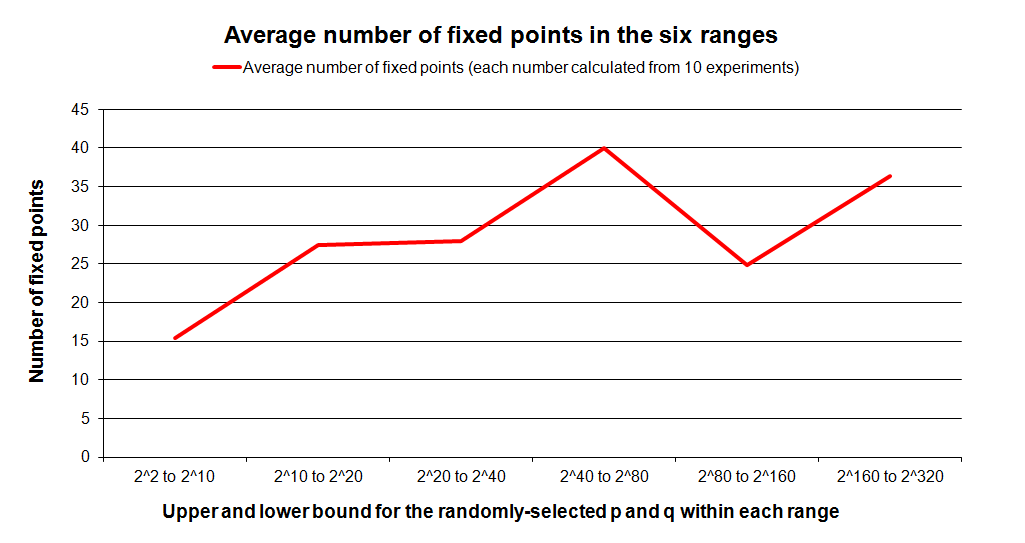
\includegraphics[width=0.92\textwidth]{figures/MAF.png}
  \caption{An empirical estimate of the quantity of fixed points for growing moduli}
  \label{fig:NumberFixpointsGrowingN}
  %\vskip +45pt
\end{figure}

Figure \ref{fig:NumberFixpointsGrowingN} shows that within the six ranges of size,
the average number of fixed points was not higher than 40.
% Unfortunately, we were unable to test the moduli for even higher ranges because 
% our Sage Program \ref{nt_sagesample_Calculate_RSA-Fixpoints}  "`Getfixpoints"'
% was too slow in ranges with $(p,q) > 2^{320}$.\\



\vspace{15pt}
% ----------------------------------------------------
\subsubsection{Example: Determining all fixed points for a specific public RSA key}

The exercise is to determine all fixed points for (n, e) = (866959, 17).\\

\noindent \textbf{Solution:} \\
We start by factoring $n$:  $ 866959 = 811 \cdot 1069$.\\

\noindent The quantity of RSA fixed points results from the theorem
\ref{nt-thm-Anzahl-RSA-Fixpunkte}:\\
$ (gcd(  p-1,  e-1)+1) \cdot (gcd(   q-1,  e-1)+1) =
  (gcd(811-1, 17-1)+1) \cdot (gcd(1069-1, 17-1)+1) = (2+1) \cdot (4+1) = 15 $\\

\noindent Sage program \ref{nt_sagesample_Calculate_RSA-Fixpoints} ``Getfixpoints''
returns the following 15 fixed points for $ (n,e) = (866959, 17)$:
\begin{table}[ht]
\begin{center}
{\tt 
\begin{tabular}{llllllll}
     0 &      1 &  23518 &  23519 &  47037 \\
188964 & 212482 & 236000 & 654477 & 843440 \\
843441 & 630959 & 677995 & 819922 & 866958 
\end{tabular} } % tt
\end{center}
\end{table}

\noindent \textbf{Example:} \\
Using $ 843441$ as a sample for validation:~~
$843441^{17} \mod 866959 = 843441$\\
So $ m = 843441$ is actually a fixed point for the given $(n,e)$.\\

\begin{sagecode}
\begin{Verbatim}%
[fontsize=\footnotesize,fontshape=tt]
import numpy

print "--- Search for fixpoints in Textbook-RSA given p, q, e ---";
fp=numpy.array([0])
fq=numpy.array([0])

#Edit e,p,q here
###EDIT BEGIN###
e=17;
p=811;
q=1069;
###EDIT END###

n=p*q;
print "Prime p: ",p;
print "Prime q: ",q;
print "Modul n: ",n;
print "Public exponent e: ", e;

r=Integers(p)
gen_f_p = r.multiplicative_generator(); print "\nGenerator of f_p: ",gen_f_p;
s=Integers(q)
gen_f_q = s.multiplicative_generator(); print "Generator of f_q: ",gen_f_q;

gcd_p = gcd(e-1,p-1)
gcd_q = gcd(e-1,q-1)
print "\ngcd(e-1,p-1): ", gcd_p;
print "gcd(e-1,q-1): ", gcd_q;

print "\nNumber of fixpoints: ",(gcd_p+1)*(gcd_q+1);
#Calculating fixpoints modulo F_p
#run i from 0 until gcd(e-1,p-1):
#g^( i*(p-1) / (gcd(e-1,p-1)) ) mod p

print "\nFixpoints modulo p";
print "0 (trivial fixpoint added manually)";
i=0;
for i in range(gcd_p):
                fix_p = power_mod(gen_f_p,Integer(i*(p-1)/gcd_p),p); print fix_p;
                fp = numpy.append(fp,fix_p)

print "\nFixpoints modulo q";
print "0 (trivial fixpoint added manually)";
j=0;
for j in range(gcd_q):
                fix_q = power_mod(gen_f_q,Integer(j*(q-1)/gcd_q),q); print fix_q;
                fq = numpy.append(fq,fix_q);

print "\nFixpoints for the public RSA key (n,e) = (", n, ",", e, ")"
for r in fp:
       for s in fq:
               print crt(Integer(r),Integer(s),Integer(p),Integer(q))

print "\nRemark: You can verify each fixpoint with power_mod(m,e,n).";
\end{Verbatim}
\caption{Determining all fixed points for a specific public RSA key}
\label{nt_sagesample_Calculate_RSA-Fixpoints}
\end{sagecode}
%#print "        Here done for the last found fixpoint:";
%#m = crt(Integer(r),Integer(s),Integer(p),Integer(q))
%#print "        m = ", m, ",", "power_mod = ", power_mod(m,e,n)
%#if (m != power_mod(m,e,n)):
%#                print "Verification failed !!!";


\vspace{60pt}
\noindent \textbf{Meaning of the Variables in the Sage Code
                  \ref{nt_sagesample_Calculate_RSA-Fixpoints}:}
\begin{Verbatim}%
[fontsize=\footnotesize,fontshape=tt]
- gen_f_p = r.multiplicative_generator()
  r is a residue class ring modulo p and multiplicative_generator() returns
  a generator element that was created by the ring modulo p.
- power_mod(gen_f_p,Integer(i*(p-1)/gcd_p),p)
  The power_mod function raises a number m to the power of e and returns the results modulo n.
  E.g.: power_mod(m, e, n) := m^e modulo n
- numpy.append(fp,power_mod(gen_f_p,Integer(i*(p-1)/gcd_p),p))
  The append function extends an array (fp) by an additional element.
- crt(Integer(r),Integer(s),Integer(p),Integer(q))
  CRT is the acronym for Chinese Remainder Theorem. crt(r, s, p, q) solves
  the congruences x = r mod p and x = s mod q with the help of the Chinese Remainder Theorem.
\end{Verbatim}

%%% xxx111222xxx-end




% ++++++++++++++++++++++++++++++++++++++++++++++++++++++++++++++++++++++++++
\newpage
\hypertarget{NumberTheory_Appendix_F}{}  %\hypertarget{AppendixListAndDef}{}
\section{Appendix: List of the definitions and theorems formulated in this chapter}
\label{l:NumberTheory_Appendix_F}{}  %\label{l:AppendixListAndDef}{}

\begin{center}
\begin{tabular}{|l|l|l|}\hline
 & Short description ~~ & Page \\ \hline

Definition~\ref{def-zth-prime} & prime numbers &  \pageref{def-zth-prime} \\
Definition~\ref{def-zth-composite} & composite numbers & \pageref{def-zth-composite}  \\ \hline

Theorem~\ref{thm-zth-cnum} & factors of composite numbers~~~~~~~ & \pageref{thm-zth-cnum}\\
Theorem~\ref{thm-zth-mthm} &  1st fundamental theorem of number theory &  \pageref{thm-zth-mthm} \\  \hline

Definition~\ref{def-zth-divisibility} & divisibility & \pageref{def-zth-divisibility} \\
Definition~\ref{def-zth-remainder} & remainder class $r$ modulo $m$ & \pageref{def-zth-remainder} \\
Definition~\ref{def-zth-congruence} & congruent & \pageref{def-zth-congruence} \\ \hline

Theorem~\ref{thm-zth-div} & congruence with difference  & \pageref{thm-zth-div} \\
Theorem~\ref{thm-zth-multinv} & multiplicative inverse (existence) & \pageref{thm-zth-multinv}  \\
Theorem~\ref{thm-zth-exhperm} & exhaustive permutation & \pageref{thm-zth-exhperm} \\
Theorem~\ref{thm-zth-pot} & power mod $m$ & \pageref{thm-zth-pot} \\ \hline

Definition~\ref{def-zth-zn} & $\mathbb{Z}_n$  & \pageref{def-zth-zn}\\
Definition~\ref{def-zth-znmult} &   $\mathbb{Z}_n^*$ & \pageref{def-zth-znmult} \\ \hline

Theorem~\ref{thm-zth-znmult} & multiplicative inverse in $\mathbb{Z}_n^*$& \pageref{thm-zth-znmult} \\ \hline

Definition~\ref{def-zth-phiofn} & Euler function $J(n)$ & \pageref{def-zth-phiofn} \\
Theorem~\ref{thm-zth-phiprime} & $J(p)$ &  \pageref{thm-zth-phiprime}\\
Theorem~\ref{thm-zth-phipq} & $J(p*q)$ &  \pageref{thm-zth-phipq}\\
Theorem~\ref{thm-zth-phimultprime} & $J(p_1 * \cdots *p_k)$ & \pageref{thm-zth-phimultprime} \\
Theorem~\ref{thm-zth-phinum} & $J(p_1^{e_1} * \cdots *p_k^{e_k})$ & \pageref{thm-zth-phinum} \\
Theorem~\ref{thm-zth-fermat1} & little Fermat  &  \pageref{thm-zth-fermat1}\\
Theorem~\ref{thm-zth-fermateuler} & Euler-Fermat theorem & \pageref{thm-zth-fermateuler} \\ \hline

Definition~\ref{def-zth-ordn} & multiplicative order $ {\rm ord}_{m} (a)$ & \pageref{def-zth-ordn} \\
Definition~\ref{def-zth-primitiveroot} & primitive root of $m$ &  \pageref{def-zth-primitiveroot}\\
Theorem~\ref{thm-zth-ordp} & exhausting of all possible values & \pageref{thm-zth-ordp} \\ \hline

Theorem~\ref{nt-thm-Anzahl-RSA-Fixpunkte} & number of RSA fixed points & \pageref{nt-thm-Anzahl-RSA-Fixpunkte} \\ \hline

\end{tabular}
\end{center}
\vskip +6 pt





% ++++++++++++++++++++++++++++++++++++++++++++++++++++++++++++++++++++++++++
% ++++++++++++++++++++++++++++++++++++++++++++++++++++++++++++++++++++++++++
\newpage
\begin{thebibliography}{99999}
\addcontentsline{toc}{section}{Bibliography}

\bibitem[Agrawal2002]{nt:Agrawal2002}  \index{Agrawal 2002} 
    M. Agrawal, N. Kayal, N. Saxena, \\
    {\em PRIMES in P}, August 2002, revised paper: \\
       \url{http://www.cse.iitk.ac.in/~manindra/algebra/primality_v6.pdf}\\
    See also the website "The AKS "PRIMES in P" Algorithm Resource":\\
       \url{http://fatphil.org/maths/AKS/}.
 
\bibitem[Bartholome1996]{nt:3Bartholome1996}  \index{Bartholome 1996} 
    A. Bartholome, J. Rung, H. Kern, \\
    {\em Zahlentheorie f\"ur Einsteiger}, Vieweg 1995, 2nd edition 1996.

\bibitem[Bauer1995]{nt:Bauer1995} \index{Bauer 1995}
    Friedrich L. Bauer, \\
    {\em Entzifferte Geheimnisse}, Springer, 1995.

\bibitem[Bauer2000]{nt:Bauer2000} \index{Bauer 2000}
    Friedrich L. Bauer, \\
    {\em Decrypted Secrets}, Springer 1997, 2nd edition 2000.

\bibitem[Bernstein2001]{nt:Bernstein2001} \index{Bernstein 2001}
    D.~J. Bernstein, \\
    {\em Circuits for integer factorization: a proposal},\\ 
    \url{http://cr.yp.to/papers/nfscircuit.ps} \\
    \url{http://cr.yp.to/djb.html}.

\bibitem[Bernstein2005]{nt:Bernstein2005} \index{ Bernstein 2005}
	Daniel J. Bernstein, \\
	{\em Factoring into coprimes in essentially linear time}, \\
	In Journal of Algorithms 54 (2005), 2005,
	\url{http://cr.yp.to/lineartime/dcba-20040404.pdf}.

\bibitem[Beutelspacher1996]{nt:Beutelspacher1996} \index{Beutelspacher 1996}
    Albrecht Beutelspacher, \\
    {\em Kryptologie}, Vieweg 1987, 5th edition 1996.

\bibitem[Bourseau2002]{nt:Bourseau2002} \index{Bourseau 2002} \index{Fox 2002}
    F. Bourseau, D. Fox, C. Thiel, \\
    {\em Vorz\"uge und Grenzen des RSA-Verfahrens},\\
    In: Datenschutz und Datensicherheit (DuD) 26/2002, pp~84-89 (see www.dud.de),\\
    \url{http://www.secorvo.de/publikationen/rsa-grenzen-fox-2002.pdf}.

\bibitem[Brands2002]{nt:Brands2002} \index{Brands 2002}
    Gilbert Brands, \\
    {\em Verschl\"usselungsalgorithmen -- Angewandte Zahlentheorie 
    rund um Sicherheitsprotokolle}, Vieweg, 2002.

\bibitem[Buchmann2004]{nt:Buchmann2004} \index{Buchmann 2004}
    Johannes Buchmann, \\
    {\em Introduction to Cryptography}, Springer, 2nd edition, 2004.

\bibitem[Buhler1993]{nt:Buhler1993} \index{Buhler 1993} 
    J.P. Buhler, H.W. Lenstra, C. Pomerance, \\
    {\em Factoring integers with the number field sieve}, \\
    In: A.K. Lenstra, H.W. Lenstra (Hrsg.): The Development of the 
    Number Field Sieve, Lecture Notes in Mathematics, vol.~1554, 
    Springer, Heidelberg 1993, pp~50$-$94.

\bibitem[Eckert2003]{nt:Eckert2003} \index{Eckert 2003}
    Claudia Eckert, \\
    {\em IT-Sicherheit: Konzepte-Verfahren-Protokolle}, 
    Oldenbourg 2001, 2nd edition 2003.

\bibitem[Ertel2001]{nt:Ertel2001} \index{Ertel 2001} 
    Wolfgang Ertel, \\
    {\em Angewandte Kryptographie}, 
    Fachbuchverlag Leipzig FV 2001.

\bibitem[Esslinger2012]{nt:Esslinger2012} \index{ Esslinger 2012}
	Esslinger, Schneider, and Simon, \\
	{\em RSA -- Sicherheit in der Praxis }, \\
	in KES -- Zeitschrift f�r Informationssicherheit,
	April 2012.


\bibitem[GISA2012]{nt:GISA2012} \index{GISA 2012}
    GISA (German Information Security Agency), \\
    {\em Recommendation for key length selection}, \\
    \url{https://www.bsi.bund.de/DE/Themen/weitereThemen/ElektronischeSignatur/TechnischeRealisierung/Kryptoalgorithmen/kryptoalgorithmen_node.html}

    BNetzA (Federal Network Agency),\\
    {\em Anually published document about algorithms and their parameters
         in the area of electronic signatures}\\
    \url{http://www.bundesnetzagentur.de/DE/Sachgebiete/QES/Veroeffentlichungen/Algorithmen/algorithmen_node.html}

    A statement on these recommendations: \\
    % \hspace*{1cm}
    \url{http://www.secorvo.de/publikationen/stellungnahme-algorithmenempfehlung-020307.pdf}.


\bibitem[Graham1994]{nt:Graham1994} \index{Graham 1994}
    Graham, Knuth, Patashnik, \\
    {\em Concrete Mathemathics, a Foundation of Computer Science}, \\
    Addison Wesley 1989, 6th printing 1994.

\bibitem[Heninger2012]{nt:Heninger2012} \index{ Heninger 2012}
	Nadia Heninger, Zakir Durumeric, Eric Wustrow, and J. Alex Halderman, \\
	{\em Mining Your Ps and Qs: Detection of Widespread Weak Keys in
        Network Devices }, \\
	August 2012, \url{https://factorable.net/paper.html}.

\bibitem[Katzenbeisser2001]{nt:Katzenbeisser2001} \index{Katzenbeisser 2001}
     Stefan Katzenbeisser, \\
     {\em Recent Advances in RSA Cryptography}, \\
     Springer 2001.

\bibitem[Kippenhahn1997]{nt:Kippenhahn1997} \index{Kippenhahn 1997}
    Rudolph Kippenhahn, \\
    {\em Verschl\"usselte Botschaften -- Geheimschrift, Enigma und Chipkarte}, 
    Rowohlt, 1997.

\bibitem[Kippenhahn1999]{nt:Kippenhahn1999} \index{Kippenhahn 1999}
    Rudolph Kippenhahn, \\
    {\em Code Breaking -- A History and Exploration}, 
    Constable, 1999.
 
\bibitem[Kleinjung2010]{nt:Kleinjung2010} \index{Kleinjung 2010}
    Thorsten Kleinjung et al.\\
    {\em Factorization of a 768-bit RSA modulus},\\
    \url{http://eprint.iacr.org/2010/006.pdf}.

\bibitem[Knuth1998]{nt:Knuth1998} \index{Knuth 1998}
    Donald E. Knuth, \\
    {\em The Art of Computer Programming, vol 2: Seminumerical Algorithms}, \\
    Addison-Wesley, 2nd edition 1998.
    % wann war erste Edition ?

\bibitem[Lenstra1993]{nt:Lenstra1993} \index{Lenstra 1993}
     A. Lenstra, H. Lenstra: \\ 
     {\em The development of the Number Field Sieve}, \\
     Lecture Notes in Mathematics 1554, Springer, New York 1993

\bibitem[Lenstra1999]{nt:Lenstra1999} Arjen K. Lenstra, Eric R. Verheul
     \index{Lenstra/Verheul 1999} \\
     {\em Selecting Cryptographic Key Sizes (1999)},\\
     Journal of Cryptology: the journal of the International 
     Association for Cryptologic Research, \\
     \url{http://www.cryptosavvy.com/cryptosizes.pdf}.
 
\bibitem[Lenstra2002]{nt:Lenstra2002} \index{Lenstra 2002}
    Arjen K. Lenstra, Adi Shamir, Jim Tomlinson, Eran Tromer,\\
    {\em Analysis of Bernstein's Factorization Circuit},\\
    \url{http://www.cryptosavvy.com/mesh.pdf}.

\bibitem[Lenstra2012]{nt:Lenstra2012} \index{ Lenstra 2012}
	Arjen K. Lenstra, James P. Hughes, Maxime Augier, Joppe W. Bos,
        Thorsten Kleinjung and Christophe Wachter, \\
	{\em Ron was wrong, Whit is right, A Sanity Check of Public Keys
             Collected on the Web}, \\
	February 2012,
	\url{http://eprint.iacr.org/2012/064.pdf}.

\bibitem[Menezes2001]{nt:Menezes2001} \index{Menezes 2001}
    Alfred J. Menezes, Paul C. van Oorschot, Scott A. Vanstone \\
    {\em Handbook of Applied Cryptography}, 
    CRC Press 1997, 5th printing 2001,\\
    \url{http://www.cacr.math.uwaterloo.ca/hac/} (Errata last updated July 24, 2011).

\bibitem[Oechslin2003]{nt:Oechslin2003} \index{ Oechslin 2003}
	Philippe Oechslin,\\
	{\em Making a Faster Cryptanalytic Time-Memory Trade-Off},\\
	At Crypto 2003, 2003,\\
	\url{http://lasecwww.epfl.ch/pub/lasec/doc/Oech03.pdf}.

\bibitem[Pfleeger1997]{nt:Pfleeger1997} \index{Pfleeger 1997}
    Charles P. Pfleeger, \\
    {\em Security in Computing}, Prentice-Hall, 2nd edition 1997.
    % im Buch stand nicht, wann die 1. Edition rauskam.

\bibitem[Pomerance1984]{nt:Pomerance1984} \index{Pomerance 1984} 
    C. Pomerance, \\
    {\em The quadratic sieve factoring algorithm}, \\
    In: G.R. Blakley, D. Chaum (Hrsg.): Proceedings of Crypto '84, 
    LNCS 196, Springer Berlin 1995, pp~169-182.

\bibitem[RSA Security 2002]{nt:RSA Security 2002} \index{RSA Security 2002} 
    RSA Security, \\
    {\em Has the RSA algorithm been compromised as a result 
    of Bernstein's Paper?}, \\
    April 8th, 2002, \\
    \url{http://www.rsasecurity.com/}.
     
\bibitem[SchneiderM2004]{nt:SchneiderM2004} \index{SchneiderM 2004} 
    Matthias Schneider, \\
    {\em Analyse der Sicherheit des RSA-Algorithmus. \\
     M\"ogliche Angriffe, deren Einfluss auf sichere Implementierungen und \"okonomische Konsequenzen}, \\
    Diploma thesis at the University of Siegen, Germany, 2004.

\bibitem[Schneier1996]{nt:Schneier1996nt} \index{Schneier 1996} 
    Bruce Schneier, \\
    {\em Applied Cryptography, Protocols, Algorithms, and Source Code in C}, \\
    Wiley and Sons, 2nd edition 1996.

\bibitem[Schulz2010]{nt:Schulz2010} \index{Schulz 2010}%\index{Time experiments}
    R.-H. Schulz, Helmut Witten, \\
    {\em Zeitexperimente zur Faktorisierung. Ein Beitrag zur Didaktik
         der Kryptographie}, 
    LogIn, no. 166/167, 2010, pp~113-120\\
    \url{http://bscw.schule.de/pub/bscw.cgi/d864899/Schulz_Witten_Zeit-Experimente.pdf}.

\bibitem[Schwenk2002]{nt:Schwenk2002}\index{Schwenk 2002}
    J\"org Schwenk, \\
    {\em Sicherheit und Kryptographie im Internet}, 
    Vieweg 2002.

\bibitem[Sedgewick1990]{nt:Sedgewick1990} \index{Sedgewick 1990}
    Robert Sedgewick,\\
    {\em Algorithms in C}, Addison-Wesley, 1990.

\bibitem[Shamir2003]{nt:Shamir2003} \index{Shamir 2003} \index{TWIRL device} 
    Adi Shamir, Eran Tromer, \\
    {\em Factoring Large Numbers with the TWIRL Device}, 
    Januar 2003, \\
    \url{http://www.wisdom.weizmann.ac.il/~tromer/}.

\bibitem[Shamir2003a]{nt:Shamir2003a} \index{Shamir 2003a} \index{TWIRL device} 
    Adi Shamir, Eran Tromer, \\
    {\em On the Cost of Factoring RSA-1024}, 
    RSA Laboratories CryptoBytes volume 6, no. 2, Summer 2003, pp~11-20, \\
    \url{http://www.rsasecurity.com/rsalabs/cryptobytes/CryptoBytes_August_2003.pdf}

\bibitem[Silverman2000]{nt:Silverman2000} \index{Silverman 2000}
     Robert D. Silverman: \\ 
     {\em A Cost-Based Security Analysis of Symmetric and Asymmetric 
          Key Lengths} \\
     In: RSA Laboratories Bulletin, no. 13, April 2000, pp~1-22

\bibitem[Stinson1995]{nt:Stinson1995} \index{Stinson 1995}
    Douglas R. Stinson,\\
    {\em Cryptography - Theory and Practice}, CRC Press, 1995.

\bibitem[Weis2003]{nt:Weis2003} \index{Weis 2003} \index{Lucks 2003} \index{Bogk 2003}
    R\"udiger Weis, Stefan Lucks, Andreas Bogk, \\
    {\em Sicherheit von 1024 bit RSA-Schl\"usseln gef\"ahrdet},\\
    In: Datenschutz und Datensicherheit (DuD) 6/2003, pp~360-362 (see www.dud.de)\\
    The article explains details about the TWIRL device\index{TWIRL device}.

\bibitem[Welschenbach2001]{nt:Welschenbach2001} \index{Welschenbach 2001}
    Welschenbach, Michael, \\
    {\em Kryptographie in C und C++}, Springer 2001.
    
\bibitem[Wiles1994]{nt:Wiles1994} \index{Wiles, Andrew}
    Wiles, Andrew, \\
    {\em Modular elliptic curves and Fermat's Last Theorem}, 
    \index{Fermat!last theorem} \\
    In: Annals of Mathematics 141 (1995).

\bibitem[Wolfenstetter1998]{nt:Wolfenstetter1998} \index{Wolfenstetter 1998}
    Albrecht Beutelspacher, J\"org Schwenk, Klaus-Dieter Wolfenstetter, \\
    {\em Moderne Verfahren in der Kryptographie}, 
    Vieweg 1995, 2nd edition 1998.

\bibitem[Yan2000]{nt:Yan2000} \index{Yan 2000} 
    Song Y. Yan, \\
    {\em Number Theory for Computing}, Springer, 2000.
\end{thebibliography}



% ++++++++++++++++++++++++++++++++++++++++++++++++++++++++++++++++++++++++++
\newpage
\section*{Web links}
\addcontentsline{toc}{section}{Web links}

\begin{enumerate}
   \item \hypertarget{knott}{}  \index{Knott, Ron}
         Ron Knott's Fibonacci \index{Fibonacci} page, \\
         Here, everything revolves around Fibonacci numbers.\\
          \url{http://www.mcs.surrey.ac.uk/personal/R.Knott/Fibonacci/fib.html}
          
   \item CrypTool, \index{CrypTool} \\
         Open source e-learning software to illustrate cryptography and
         cryptanalysis\\
          \url{http://www.cryptool.de}, \\
          \url{http://www.cryptool.org},\\ 
          \url{http://www.cryptool.com}
          
   \item Mathematica, \index{Mathematica} \\
         Commercial mathematics package \\
         \url{http://www.wolfram.com}
          
   \item LiDIA, \index{LiDIA} \\
         Extensive library containing number-theory functions and the
         LC interpreter. Maintenance stopped. \\
          \url{http://www.informatik.tu-darmstadt.de/TI/LiDIA}
          
   \item BC, \index{BC} \\
         Interpreter with number-theory functions \\
         \url{http://www.gnu.org/software/bc/bc.html}
          
   \item Pari-GP, \index{Pari-GP} \\
         Excellent, fast, free interpreter with number theoretical functions.\\
         \url{http://pari.math.u-bordeaux.fr/} \\
         \url{http://en.wikipedia.org/wiki/PARI/GP} \\
         Resources for PARI/GP at Karim Belabas's website:\\
         \url{http://www.math.u-bordeaux.fr/~belabas/pari/}
           
   \item \index{Munchenbach@M\"unchenbach, Carsten}
         Only after I had completed this article, did I come across the
         website of Mr.\ M\"unchenbach, which interactively and didactically
         uses elementary number theory to provide a sophisticated
         description of the fundamental mathematical thought processes. 
         It was created for a teaching project in the 11th grade of the
         technical grammar school (unfortunately only available in German): \\
         \url{http://www.hydrargyrum.de/kryptographie}
                      
   \item Web site of Mr.~Wagner, who is responsible for the development
	 of the curriculum of computer science in one of the German federal 
         states (L\"ander). Here you can get hold of a collection of texts
	 and (Java-)\discretionary{}{}{}programs (available only in German):\\
         \url{http://www.saar.de/~awa/kryptolo.htm}
          
   \item GISA, \index{GISA} \\
         German Information Security Agency \\
         \url{http://www.bsi.bund.de}

   \item Factorization records and challenges\index{Factorization!factoring records},\\
         \url{http://www.crypto-world.com/} \\
         \url{http://www.crypto-world.com/FactorWorld.html}, Webseite von Scott Contini \\
         \url{http://www.loria.fr/~zimmerma/records/factor.html} \\

         \url{http://www.tutorgig.com/ed/RSA\_number} \\

         \url{http://www.uni-bonn.de/Aktuelles/Pressemitteilungen/pm02/pm035-02.html} \\
         \url{http://www.ercim.org/publication/Ercim\_News/enw49/franke.html} \\ %2002-01
         \url{http://www.loria.fr/~zimmerma/records/rsa160} \\

         \url{http://www.rsa.com/rsalabs/node.asp?id=2092}
	 

   \item The Cunningham Project, \index{Cunningham project}\\ 
         \url{http://www.cerias.purdue.edu/homes/ssw/cun/}


   \item Sage, \index{Sage} \\
         Excellent, open source computer algebra system with Python as script
         language, used to build the code samples in this chapter.
	 See the introduction in chapter~\ref{s:appendix-using-sage}.\\
         \url{http://www.sagemath.org/} \\
         \url{http://en.wikipedia.org/wiki/Sage_%28mathematics_software%29}

\end{enumerate}



% ++++++++++++++++++++++++++++++++++++++++++++++++++++++++++++++++++++++++++
\vskip +20 pt
\section*{Acknowledgments}
\addcontentsline{toc}{section}{Acknowledgments}

I would like to take this opportunity to thank 
\begin{itemize}

  \item {Henrik Koy for making many very useful suggestions, 
         for the very constructive proof-reading of the first version of
	 this article, and for helping with TeX.}

  \item {J\"org Cornelius Schneider for his enthusiastic TeX support and for the
         many cases where he helped when facing programming or design problems.}
  
  \item {Dr.\ Georg Illies for pointing me to Pari-GP\index{Pari-GP}.}
  
  \item {Lars Fischer for his help with fast Pari-GP\index{Pari-GP} code for
        primitive roots.}
  
  \item {Minh Van Nguyen from Australia for his always fast, professional and exhaustive
         help with the first Sage\index{Sage} code samples in this chapter.}

\end{itemize}



% Local Variables:
% TeX-master: "../script-en.tex"
% End:

\renewcommand{\CTBChapName}{(Chap ModernCrypto)}  % $Id$
\setcounter{satz}{0}
\setcounter{definition}{0}

\newcommand{\NT}{\vspace*{0.2\baselineskip}\\}
\newcommand{\HZ}{\vspace*{0.5\baselineskip}}
\newcommand{\R}{\text{I}\!\text{R}}
\newcommand{\N}{\text{I}\!\text{N}}
\newcommand{\Q}{\text{Q}\!\!\!\text{l}\,\,}
\newcommand{\C}{\text{C}\!\!\!\text{l}\,\,}
\newcommand{\K}{\text{I}\!\text{K}}
\newcommand{\Z}{\mathbf{\mathbb{Z}}}
%--------------------------------------- matheScript-Zeichen definieren
\newcommand{\fs}{\mathscr{F}}  
\newcommand{\es}{\mathscr{E}}  
\newcommand{\cs}{\mathscr{C}}  
\newcommand{\gs}{\mathscr{G}}
\newcommand{\is}{\mathscr{I}}
\newcommand{\os}{\mathscr{O}}
\newcommand{\ks}{\mathscr{K}}
\newcommand{\qs}{\mathscr{Q}}
\newcommand{\us}{\mathscr{U}}
\newcommand{\hs}{\mathscr{H}}
\newcommand{\ps}{\mathscr{P}}
\newcommand{\as}{\mathscr{A}}
\newcommand{\rs}{\mathscr{R}}
\newcommand{\bs}{\mathscr{B}}
%-------------------------------------
\newcommand{\PG}{\text{I}\!\text{P}}
\newcommand{\carre}{\square}
\newcommand{\ncarre}{/\negthickspace\negthickspace\square}
\newcommand{\ncarreq}{{\ncarre}_q}
\newcommand{\ncarree}{/\negthickspace\negthickspace\negthickspace\square}
\newcommand{\ncarrepi}{{\ncarre}_{p^i}}
\newcommand{\mc}[1]{{\cal #1}}
\newcommand{\Char}{\text{char}}
\newcommand{\Aut}{\text{Aut}}
\newcommand{\Fix}{\text{Fix}}
\newcommand{\Syl}{\text{Syl}}
\newcommand{\Bild}{\text{Bild}}
\newcommand{\ggt}{\text{ggT}}
\newcommand{\kgv}{\text{kgV}}
\newcommand{\Id}{\text{Id}}
\newcommand{\nqcarre}{{\ncarre}_{q^2}}

\setlength{\fboxrule}{.4pt}
\setlength{\fboxsep}{4pt}


\newpage
%********************************************************************
\hypertarget{Chapter_ModernCryptography}{}
\chapter[Die mathematischen Ideen hinter der modernen Kryptographie]
        {Die mathematischen Ideen hinter der modernen Kryptographie\footnotemark}
\footnotetext{%
    \index{ZT, Lernprogramm Zahlentheorie}%
    \index{Lernprogramm ZT}%
    Mit dem Lernprogramm {\bf ZT} k�nnen Sie spielerisch einige der hier
    besprochenen Verfahren (RSA, Rabin, DH, ElGamal) nachvollziehen
    (siehe Lern-Kapitel 4.2 und 4.3, Seiten 9-17/17).\\
    ZT k�nnen Sie in CrypTool\index{CrypTool} �ber das Men�
    {\bf Einzelverfahren \textbackslash{} Zahlentheorie 
    interaktiv \textbackslash{} Lernprogramm f�r Zahlentheorie} aufrufen.
    Siehe Anhang \ref{s:appendix-Learn-NT}.
}
\label{Chapter_ModernCryptography}
%********************************************************************
(Oyono R./ Esslinger B./ Schneider J., Sep. 2000;
           Updates Nov. 2000, Feb. 2003, Apr. 2007, M�rz 2010)


\vskip +30 pt

\begin{center}
\fbox{\parbox{15cm}{
   {\em Georg Christoph Lichtenberg\footnotemark:}\\
   Ich wei� nicht, ob es besser wird, wenn wir es �ndern,\\
   aber ich wei�, dass wir es �ndern m�ssen, wenn es besser werden soll.\\

   {\em Anmerkung von Unbekannt (Radio) dazu:}\\
   Und Gott gebe den Akteuren bei der notwendigen Umsetzung\\
   das Wissen, die Weisheit und das Verantwortungsbewusstsein,\\
   zwischen Aktionismus, Selbstdarstellung und planvollem Handeln\\
   zu unterscheiden -- und ihr Wissen auch anzuwenden.
}}
\end{center}
\footnotetext{%
  Georg Christoph Lichtenberg\index{Lichtenberg, Georg Christoph}, 
  deutscher Schriftsteller und Physiker (1742-1799),\\ 
  (siehe auch: \href{http://de.wikipedia.org/wiki/Georg\_Christoph\_Lichtenberg}
                {\tt http://de.wikipedia.org/wiki/Georg\_Christoph\_Lichtenberg})
}

%--------------------------------------------------------------------
\hypertarget{OneWayFunktion1}{}
\section{Einwegfunktionen mit Fallt�r und Komplexit�tsklassen}
\label{OneWayFunktion1}
%--------------------------------------------------------------------
\index{Kryptographie!moderne} \index{Einwegfunktion}
Eine {\bf Einwegfunktion} ist eine effizient zu 
berechnende Funktion, deren Umkehrung jedoch nur mit 
extrem hohem Rechenaufwand -- jedoch praktisch unm�glich -- zu berechnen ist.\par

Etwas genauer formuliert:  Eine Einwegfunktion ist eine Abbildung $ f $ einer Menge $ X $ in eine Menge $ Y, $ so dass $ f(x) $ f�r jedes Element $ x $ von $ X $ leicht zu berechnen ist, w�hrend es f�r (fast) jedes $ y $ aus $ Y $  praktisch unm�glich ist, ein Urbild $ x $ (d.h. ein $ x $ mit $ f(x)=y $) zu finden.\par

Ein allt�gliches Beispiel f�r eine Einwegfunktion ist ein Telefonbuch: die auszuf�hrende Funktion ist die, einem Namen die entsprechende Telefonnummer zuzuordnen. Da die Namen alphabetisch geordnet sind, ist diese Zuordnung einfach auszuf�hren. Aber ihre Invertierung, also die Zuordnung eines Namens zu einer gegebenen Nummer, ist offensichtlich schwierig, wenn man nur ein Telefonbuch zur Verf�gung hat. \par

Einwegfunktionen spielen in der Kryptographie eine entscheidende Rolle. Fast alle kryptographischen Begriffe kann man durch Verwendung des Begriffs Einwegfunktion umformulieren. Als Beispiel betrachten wir die Public-Key-Verschl�sselung \index{Verschl�sselung!Public-Key} (asymmetrische Kryptographie):\par

Jedem Teilnehmer $ T $ des Systems wird ein privater \index{Schl�ssel!privat}
\index{Schl�ssel!�ffentlich} Schl�ssel $d_T$~\mbox{und} ein sogenannter �ffentlicher Schl�ssel $ e_T $   zugeordnet. Dabei muss die folgende Eigenschaft (Public-Key-Eigen"-schaft) gelten:\\
F�r einen Gegner, der den �ffentlichen Schl�ssel $ e_T $  kennt, ist es praktisch unm�glich, den privaten Schl�ssel  $ d_T $ zu bestimmen.\par

Zur Konstruktion n�tzlicher Public-Key-Verfahren sucht man also eine Einwegfunktion, die in einer Richtung \glqq einfach\grqq {} zu berechnen, die in der anderen Richtung jedoch \glqq schwer\grqq {} (praktisch unm�glich) zu berechnen ist, solange eine bestimmte zus�tzliche Information \index{Einwegfunktion!mit Fallt�r} (Fallt�r) nicht zur Verf�gung steht. Mit der zus�tzlichen Information kann die Umkehrung effizient gel�st werden. Solche Funktionen nennt man {\bf Einwegfunktionen mit Fallt�r} (trapdoor one-way function). Im obigen Fall ist $ d_T $ die Fallt�r-In"-for"-ma"-tion. \par

Dabei bezeichnet man ein Problem als \glqq einfach\grqq, wenn es in \index{Laufzeit!polynomial} \index{Polynom} polynomialer Zeit als Funktion der L�nge der Eingabe l�sbar ist, d.h. wenn es so gel�st werden kann, dass der Zeitaufwand sich als polynomiale Funktion in Abh�ngigkeit der L�nge der Eingabe darstellen l�sst. 
Wenn die L�nge der Eingabe $ n $ Bits betr�gt, so ist die Zeit der Berechnung der Funktion proportional zu $ n^{a}, $ wobei $ a $  eine Konstante ist. Man sagt, dass die \index{Komplexit�t} Komplexit�t solcher Probleme $ O(n^{a}) $ betr�gt (Landau- oder Big-O-Notation). 

Vergleicht man 2 Funktionen  $ 2^n $  und   $ n^{a} $, wobei $ a $  
eine Konstante ist, dann gibt es immer einen Wert f�r  $ n $, ab dem
f�r alle weiteren $ n $ gilt: $ n^{a}  <  2^n $. 
Die Funktion  $ n^{a} $  hat eine geringere Komplexit�t.
Z.B. f�r $ a=5 $ gilt: ab der L�nge $ n=23 $ ist 
$ 2^n > n^5 $ ~\mbox{und} danach w�chst $ 2^n $ auch deutlich 
schneller \
[($ 2^{22}= 4.194.304 $, $ 22^5= 5.153.632 $), \
 ($ 2^{23}= 8.388.608 $, $ 23^5= 6.436.343 $), \
 ($ 2^{24}=16.777.216 $, $ 24^5= 7.962.624 $)].\par 
% "\mbox" nur, weil bei Ausdruck bei be die Blanks stets falsch sa�en:
%  "n^5un d"

Der Begriff \glqq praktisch unm�glich\grqq {} ist etwas schwammiger. 
Allgemein kann man sagen, ein Problem ist \index{Laufzeit!effizient}
nicht effizient l�sbar, wenn der zu seiner L�sung ben�tigte Aufwand
schneller w�chst als die polynomiale \index{Polynom} Zeit als Funktion der Gr��e der
Eingabe. Wenn beispielsweise die L�nge der Eingabe $ n $  Bits betr�gt
und die Zeit zur Berechnung der Funktion proportional zu $ 2^n $ ist, 
so gilt gegenw�rtig: die Funktion ist f�r $n > 80$ praktisch nicht zu 
berechnen.

Die Entwicklung eines praktisch einsetzbaren Public-Key-Verfahrens h�ngt daher von der Entdeckung einer geeigneten Einwegfunktion mit Fallt�r ab.\par

Um Ordnung in die verwirrende Vielfalt von m�glichen Problemen und ihre Komplexit�ten zu bringen, fasst man Probleme mit �hnlicher Komplexit�t zu Klassen zusammen.

Die wichtigsten Komplexit�tsklassen  sind die Klassen \textbf{P} und \textbf{NP}: 

\begin{itemize}

    \item Die Klasse \textbf{P}: Zu dieser Klasse geh�ren diejenigen Probleme, die mit polynomialem \index{Polynom} Zeitaufwand l�sbar sind.
    
    \item Die Klasse \textbf{NP}: Bei der Definition dieser Klasse betrachten wir nicht den Aufwand zur L�sung eines Problems, sondern den Aufwand zur Verifizierung einer gegebenen L�sung. Die Klasse \textbf{NP} besteht aus denjenigen Problemen, bei denen die Verifizierung einer gegebenen L�sung mit polynomialem Zeitaufwand m�glich ist. Dabei bedeutet der Begriff \textbf{NP} \glqq nichtdeterministisch\grqq {} polynomial \index{Polynom} und bezieht sich auf ein Berechnungsmodell, d.h. auf einen nur in der Theorie existierenden Computer, der richtige L�sungen nichtdeterministisch \glqq raten\grqq {} und dies dann in polynomialer Zeit verifizieren kann.

\end{itemize}

Die Klasse \textbf{P} ist in der Klasse \textbf{NP} enthalten. Ein ber�hmtes offenes Problem ist die Frage, ob $ \textbf{P} \neq \textbf{NP} $ gilt oder nicht, d.h. ob \textbf{P} eine echte Teilmenge ist oder nicht. Eine wichtige Eigenschaft der Klasse \textbf{NP} ist, dass sie auch sogenannte \glqq \textbf{NP}-vollst�ndige\grqq {} Probleme enth�lt. Dies sind Probleme, welche die Klasse \textbf{NP} im Folgenden Sinne vollst�ndig repr�sentieren: Wenn es einen \glqq guten\grqq {} Algorithmus f�r ein solches Problem gibt, dann existieren f�r alle Probleme aus \textbf{NP} \glqq gute\grqq {} Algorithmen. Insbesondere gilt: wenn auch nur ein vollst�ndiges Problem in \textbf{P} l�ge, d.h. wenn es einen polynomialen \index{Polynom} L�sungsalgorithmus f�r dieses Problem g�be, so w�re \textbf{P}=\textbf{NP}. In diesem Sinn sind die \textbf{NP}-vollst�ndigen Probleme die schwierigsten Probleme in \textbf{NP}.

Viele kryptographische Protokolle sind so gemacht, dass die \glqq guten\grqq {} Teilnehmer nur Probleme aus \textbf{P} l�sen m�ssen, w�hrend sich ein Angreifer vor Probleme aus \textbf{NP} gestellt sieht.

Man wei� leider bis heute nicht, ob es Einwegfunktionen �berhaupt gibt. Man kann aber zeigen, dass Einwegfunktionen genau dann existieren, wenn $ \textbf{P} \neq \textbf{NP} $ gilt \cite[S.63]{mc:Balcazar1988}.
\vskip +5pt

Immer wieder behauptete jemand, er habe die �quivalenz bewiesen
(z.B.  \cite{mc:Hesselink2001}), %%Hinweis wegen geocities per he.pa, 16.2.2010
aber bisher erwiesen sich diese Aussagen stets als falsch.

Es wurden eine Reihe von Algorithmen f�r Public-Key-Verfahren vorgeschlagen. Einige davon erwiesen sich, obwohl sie zun�chst vielversprechend erschienen, als polynomial \index{Polynom} l�sbar. Der ber�hmteste durchgefallene Bewerber ist der von Ralph Merkle \cite{mc:Merkle1978} vorgeschlagene Knapsack mit Fallt�r.


%\newpage
\vskip +20 pt
%--------------------------------------------------------------------
\section{Knapsackproblem als Basis f�r Public-Key-Verfahren}
\index{Kryptographie!Public-Key}
%--------------------------------------------------------------------

%--------------------------------------------------------------------
\subsection{Knapsackproblem} \index{Knapsack}

Gegeben $ n $ Gegenst�nde $ G_1, \dots, G_n $ mit den Gewichten $ g_1, \dots g_n $ und den Werten $w_1, \cdots, w_n. $ Man soll wertm��ig so viel wie m�glich unter Beachtung einer oberen Gewichtsschranke $ g $ davontragen. Gesucht ist also eine Teilmenge von $ \{ G_1, \cdots,G_n\}, $ etwa $ \{G_{i_1}, \dots ,G_{i_k} \}, $ so dass  $ w_{i_1}+ \cdots +w_{i_k} $ maximal wird unter der Bedingung $  g_{i_1}+ \cdots +g_{i_k} \leq g. $ \par
Derartige Fragen sind sogenannte {\bf NP}-vollst�ndige Probleme (nicht \index{Laufzeit!nicht polynomial NP} deterministisch polynomial\index{Polynom}), die aufwendig zu berechnen sind.\index{Knapsack}

Ein Spezialfall des Knapsackproblems ist:\\
Gegeben sind die nat�rlichen Zahlen $ a_1, \dots, a_n $   und $ g .$
Gesucht sind  $ x_1, \dots, x_n \in \{ 0,1\} $  mit $ g = \sum_{i=1}^{n}x_i a_i $  (wo also $ g_i = a_i = w_i $ gew�hlt ist).
Dieses Problem hei�t auch  {\bf 0-1-Knapsackprob"-lem} und wird mit $ K(a_1, \dots, a_n;g) $  bezeichnet.\\

Zwei 0-1-Knapsackprobleme  $ K(a_1, \dots, a_n;g) $   und
$ K(a'_1, \dots, a'_n;g') $  hei�en kongruent, falls es zwei
teilerfremde\index{Zahlen!teilerfremde (co-prime)} Zahlen $ w $ und $ m $
gibt, so dass
\begin{enumerate}
    \item $ m > \max \{ \sum_{i=1}^n a_i , \sum_{i=1}^n a'_i \}, $

    \item $ g \equiv wg' \mod m, $

    \item $ a_i \equiv w a'_i \mod m $ f�r alle $ i=1, \dots, n.$

\end{enumerate}
 
\begin{remark}{:}\\
Kongruente 0-1-Knapsackprobleme haben dieselben L�sungen.
Ein schneller Algorithmus zur Kl�rung der Frage, ob zwei 0-1-Knapsackprobleme kongruent sind, ist nicht bekannt.
\end{remark}

Das L�sen eines 0-1-Knapsackproblems kann durch Probieren der $ 2^n $   M�glichkeiten f�r $ x_1, \dots, x_n $   erfolgen. Die beste Methode erfordert $ O(2^{n/2}) $  Operationen, was f�r $ n=100 $  mit $ 2^{100} \approx 1,27 \cdot 10^{30} $  und  $ 2^{n/2} \approx 1,13 \cdot 10^{15} $ f�r Computer eine un�berwindbare H�rde darstellt.
Allerdings ist die L�sung f�r spezielle $ a_1, \dots, a_n $   recht einfach zu finden, etwa f�r $ a_i = 2^{i-1}. $  Die bin�re Darstellung von $ g $ liefert unmittelbar $ x_1, \dots, x_n$. Allgemein ist die L�sung des 0-1-Knapsackproblems leicht zu finden, falls eine \index{Permutation} Permutation\footnote{Eine Permutation\index{Permutation} $\pi$ der Zahlen $1, \dots, n$ ist die Vertauschung der Reihenfolge, in der
diese Zahlen aufgez�hlt werden. Beispielsweise ist eine Permutation $\pi$ von $(1,2,3)$ gleich $(3,1,2),$ also $\pi(1) = 3$, $\pi(2) =1$ 
und $\pi(3) = 2$.} 
$ \pi $  von $ 1, \dots, n $  mit $ a_{\pi (j)} > \sum_{i=1}^{j-1} a_{\pi(i)} $  existiert. Ist zus�tzlich $ \pi $ die Identit�t, d.h. $ \pi(i)=i $ f�r $ i=1,2,\dots,n, $ so hei�t die Folge $ a_1, \dots , a_n $ superwachsend.
Das Verfahren \ref{knapsackalgo} l�st das Knapsackproblem mit superwachsender Folge im Zeitraum von $ O(n). $
\begin{cryptoprocedure}
\begin{tabbing}
\hspace*{0.5cm} \= \hspace*{0.5cm} \= \hspace*{0.5cm} \= \kill
\>{\bf for} $ i=n $ {\bf to} 1 {\bf do} \\
\>\> {\bf if} $ T\geq a_i $ {\bf then}\\
\>\> \> $ T:=T-s_i $ \\
\>\>\> $ x_i:=1 $ \\
\>\> {\bf else} \\
\>\>\> $ x_i:=0 $\\
\>{\bf if} $ T=0 $ {\bf then} \\
\>\> $ X:=(x_1, \dots, x_n) $ ist die L�sung. \\
\>{\bf else} \\
\>\> Es gibt keine L�sung.
\end{tabbing}
\caption{L�sen von Knapsackproblemen mit superwachsenden Gewichten}
\label{knapsackalgo}
\end{cryptoprocedure}


%--------------------------------------------------------------------
\subsection{Merkle-Hellman Knapsack-Verschl�sselung}
\index{Hellman, Martin} \index{Merkle, Ralph} 

1978 gaben Merkle und Hellman \cite{mc:Merkle1978} \index{Verschl�sselung!Merkle-Hellman} ein Public-Key-Verschl�sselungs-Verfahren an, das darauf beruht, das leichte 0-1-Knapsackproblem mit einer superwachsenden Folge in ein kongruentes mit einer nicht superwachsenden Folge zu \glqq verfremden\grqq. Es ist eine Blockchiffrierung, die bei jedem Durchgang einen $n$ Bit langen Klartext chiffriert, siehe Krypto-Verfahren \ref{merklehellmanproc}.
\index{Knapsack!Merkle-Hellman}

\begin{cryptoprocedure}
Es sei $ (a_1, \dots, a_n) $ superwachsend. Seien $ m $ und $ w $ zwei
teilerfremde\index{Zahlen!teilerfremde (co-prime)} Zahlen mit $ m >
\sum_{i=1}^{n} a_i $ und $ 1\leq w \leq m-1. $
W�hle $\bar{w} $ mit $ w \bar{w} \equiv 1 \mod m $ die modulare Inverse
von $ w $ und setze $ b_i:= wa_i \mod m, $ $ 0\leq b_i < m $ f�r $ i=1,
\dots ,n, $ und pr�fe, ob die Folge $ b_1, \dots b_n $ nicht superwachsend
ist. Danach wird eine Permutation $ b_{\pi (1)}, \dots , b_{\pi(n)} $
von $ b_1, \dots , b_n $ publiziert und insgeheim die zu $ \pi $ inverse
Permutation $ \mu $ festgehalten. Ein Sender schreibt seine Nachricht
in Bl�cke $ (x_1^{(j)}, \dots, x_n^{(j)}) $ von Bin�rzahlen der L�nge
$ n $ und bildet \[ g^{(j)}:= \sum_{i=1}^n x_{i}^{(j)} b_{\pi(i)} \]
und sendet $ g^{(j)}, (j=1,2, \dots). $\par
Der Schl�sselinhaber bildet
\[ G^{(j)}:=\bar{w} g^{(j)} \mod m ,\quad 0 \leq G^{(j)} < m \]
und verschafft sich die $ x_{\mu(i)}^{(j)} \in \{ 0,1\} $ (und somit auch die $ x_i^{(j)} $) aus
\begin{eqnarray*}
G^{(j)} & \equiv & \bar{w} g^{(j)} = \sum_{i=1}^n x_i^{(j)} b_{\pi (i)} \bar{w} \equiv \sum_{i=1}^n x_i^{(j)} a_{\pi (i)} \mod m \\
& = & \sum_{i=1}^n x_{\mu (i)}^{(j)} a_{\pi (\mu (i))} = \sum _{i=1}^n x_{\mu (i)}^{(j)} a_i \mod m, 
\end{eqnarray*}
indem er die leichten 0-1-Knapsackprobleme $ K(a_1,\dots,a_n;G^{(j)}) $ mit superwachsender Folge $ a_1, \dots,a_n $ l�st.
\caption{Merkle-Hellman (auf Knapsackproblemen basierend)}
\label{merklehellmanproc}
\end{cryptoprocedure}



1982 gab \index{Shamir, Adi} Shamir \cite{mc:Shamir1982} einen Algorithmus zum
Brechen des Systems in polynomialer \index{Polynom} Zeit an, ohne das allgemeine
Knapsackproblem zu l�sen. Len \index{Adleman, Leonard} Adleman
\cite{mc:Adleman1982} und Jeff Lagarias \index{Lagarias, Jeff}
\cite{mc:Lagarias1983} gaben einen Algorithmus zum Brechen des 2-fachen
iterierten Merkle-Hellman Knapsack-Verschl�sselungsver"-fah"-rens in
polynomialer Zeit an. Ernst Brickell \index{Brickell, Ernst}
\cite{mc:Brickell1985} gab schlie�lich einen Algorithmus zum Brechen des
mehrfachen iterierten Merkle-Hellman Knapsack-Verschl�sselungs"-ver"-fah"-ren in
polynomialer Zeit an. Damit war dieses Verfahren als
Verschl�sse"-lungs"-ver"-fah"-ren ungeeignet. Dieses Verfahren liefert also eine
Einwegfunktion, deren Fallt�r-In"-for"-ma"-tion (Verfremden des
0-1-Knapsackproblems) durch einen Gegner entdeckt werden k�nnte.


%---------------------------------------------------------------------
\section{Primfaktorzerlegung als Basis f�r Public-Key-Verfahren}
\index{Primfaktor!Zerlegung}
%--------------------------------------------------------------------

%--------------------------------------------------------------------
\hypertarget{RSAVerfahren}{}
\subsection[Das RSA-Verfahren]
{Das RSA-Verfahren\footnote{%
Vergleiche auch die Kapitel \ref{rsabeweis}, ff.
}$^,$\footnote{%
Mit CrypTool\index{CrypTool} k�nnen Sie praktische Erfahrungen
mit dem RSA-Verfahren sammeln: per Men� {\bf Einzelverfahren 
\textbackslash{} RSA-Kryptosystem \textbackslash{} RSA-Demo}.
}}
\index{RSA} \label{rsaverfahren}

Bereits 1978 stellten R. \index{Rivest, Ronald} Rivest,
\index{Shamir, Adi} A. Shamir,  \index{Adleman, Leonard} L. Adleman
\cite{mc:RSA1978} das bis heute wichtigste 
asymmetrische Kryptographie-Verfahren vor (Krypto-Verfahren~\ref{rsaproc}).

\index{Faktorisierung!Faktorisierungsproblem}
\index{Eulersche Phi-Funktion}
\begin{cryptoprocedure}
\textbf{Schl�sselgenerierung:}

Seien $p$ und $q$ zwei verschiedene Primzahlen und $N=pq.$ Sei $e$ eine frei w�hlbare, zu $ \phi (N) $ \index{Primzahl!relative} relative Primzahl, d.h. $ \ggt (e,\phi (N))=1. $ Mit dem Euklidschen Algorithmus berechnet man die nat�rliche Zahl  $ d < \phi (N), $ so dass gilt

\[ ed \equiv 1 \mod \phi (N). \]
Dabei ist $ \phi $ die {\bf Eulersche Phi-Funktion}. 

Der Ausgangstext wird in Bl�cke zerlegt und verschl�sselt, wobei jeder Block einen bin�ren Wert $ x^{(j)} \leq N $ hat. \vskip + 5 pt

\textbf{�ffentlicher Schl�ssel:}
\[ N,e. \]
\textbf{Privater Schl�ssel:}
\[ d. \]
\textbf{Verschl�sselung:}
\[ y= e_{T} (x) = x^{e} \mod N.\]
\textbf{Entschl�sselung:}
\[ d_{T} (y) = y^d \mod N \]
\caption{RSA (auf dem Faktorisierungsproblem basierend)}
\label{rsaproc}
\end{cryptoprocedure}

\begin{remark}{:}\\
Die Eulersche Phi-Funktion ist definiert duch:
$ \phi (N)$ ist die Anzahl der zu $ N $ {} teilerfremden nat�rlichen
Zahlen $ x \leq N. $ Zwei nat�rliche Zahlen $ a $ und $ b $ sind
teilerfremd\index{Zahlen!teilerfremde (co-prime)}, falls $ \ggt (a,b)=1. $

F�r die Eulersche Phi-Funktion gilt: 
\[ \phi (1)=1,~\phi(2)=1,
~\phi(3)=2, ~\phi (4)=2, ~\phi(6)=2, ~\phi (10)= 4, ~\phi (15)=8.
\]
Zum Beispiel ist $ \phi (24)=8, $ weil 
\[
|\{ x <24 : \ggt (x,24) =1 \}| =|\{1,5,7,11,13,17,19,23\}|.
\]
Ist  $ p $ eine Primzahl, so gilt $ \phi (p)= p-1. $\\
Kennt man die verschiedenen Primfaktoren  $ p_1, \dots , p_k $ von $ N, $ so ist 
\[
\phi (N) = N \cdot (1-\frac{1}{p_1}) \,
\cdots \, (1-\frac{1}{p_k}).\footnote{%
Weitere Formeln zur Eulerschen Phi-Funktionfinden sich in \ref{L-Euler-Function}.}
\]
Tabelle~\ref{phi15} zeigt die Werte bis $15$. Im Spezialfall $ N=pq $ gilt
\[
\phi (N)= pq(1-1/p)(1-1/q) = p(1-1/p)q(1-1/q)=(p-1)(q-1).
\]
\end{remark}
\begin{table}[ht]
\begin{center}
\begin{tabular}{|l|l|l|}\hline
$n$ & $\phi (n) $ & Die zu $ n $ teilerfremden\index{Zahlen!teilerfremde
(co-prime)} nat�rlichen Zahlen kleiner $ n. $ \\ \hline
1 & 1 & 1  \\
2 & 1 & 1 \\
3 &  2 & 1, 2 \\ 
4 &  2 & 1, 3 \\ 
5 &  4 & 1, 2, 3, 4 \\ 
6 &  2 & 1, 5 \\ 
7 &  6 & 1, 2, 3, 4, 5, 6 \\ 
8 &  4 & 1, 3, 5, 7 \\ 
9 &  6 & 1, 2, 4, 5, 7, 8 \\ 
10 &  4 & 1, 3, 7, 9 \\ 
15 &  8 & 1, 2, 4, 7, 8, 11, 13, 14 \\ \hline
\end{tabular}
\end{center}
\caption{Eulersche Phi-Funktion}
\label{phi15}
\end{table}

Die Funktion $ e_T $  ist eine Einwegfunktion, deren Fallt�r-Information die Primfaktorzerlegung von $ N $ ist.

Zur Zeit ist kein Algorithmus bekannt, der das Produkt zweier Primzahlen bei sehr gro�en Werten geeignet schnell
zerlegen kann (z.B. bei mehreren hundert Dezimalstellen). Die heute schnellsten bekannten Algorithmen \cite{mc:Stinson1995} zerlegen eine 
zusammengesetzte ganze Zahl $ N $ in einem Zeitraum proportional zu  
$ L(N)= e^{\sqrt{\ln (N) \ln (\ln (N))}}. $ Einige Beispielwerte finden sich in Tabelle~\ref{lnvalues}.
\begin{table}[ht]
\begin{center}
\begin{tabular}{|l||l|l|l|l|l|l|}\hline
$N$ & $ 10^{50} $ & $ 10^{100} $ & $ 10^{150} $ & $ 10^{200} $ & $ 10^{250} $ & $ 10^{300} $ \\ \hline
$L(N)$ & $ 1,42 \cdot 10^{10} $ &  $ 2,34  \cdot 10^{15} $ &  $ 3,26 \cdot 10^{19} $ &  $ 1,20 \cdot 10^{23} $ &  $ 1,86 \cdot 10^{26} $ &  $ 1,53 \cdot 10^{29} $ \\ \hline
\end{tabular}
\end{center}
\caption{Wertetabelle $L(N)$}
\label{lnvalues}
\end{table}

Bewiesen ist bis heute nicht, dass das Problem, RSA zu brechen, �quivalent zum
Faktorisierungsproblem \index{Faktorisierung!Faktorisierungsproblem} ist. Es ist
aber klar, dass wenn das Faktorisierungsproblem \glqq gel�st\grqq {} ist, dass
dann das RSA-Verfahren nicht mehr sicher ist.\footnote{%
Im Jahre 2000 waren die Autoren der Ansicht, dass Werte der
Gr��enordnung $ 100 $ bis $ 200 $ Dezimalstellen sicher sind. Sie sch�tzten,
dass mit der aktuellen Computertechnik eine Zahl mit $100$
Dezimalstellen bei vertretbaren Kosten in etwa zwei Wochen zerlegt werden
k�nnte, dass mit einer teuren Konfiguration (z.B. im Bereich von 10 Millionen
US-Dollar) eine Zahl mit $150$ Dezimalstellen in etwa einem Jahr zerlegt
werden k�nnte und dass eine $200$-stellige Zahl noch f�r eine sehr lange Zeit
unzerlegbar bleiben d�rfte, falls es zu keinem mathematischen Durchbruch kommt.
Dass es aber nicht doch schon morgen zu einem mathematischen Durchbruch kommt,
kann man nie ausschlie�en.\\
Wie leicht man sich versch�tzen kann, zeigt die
\hyperlink{RSA-200-chap3}{Faktorisierung von RSA-200} 
(siehe Kapitel \ref{nt:NoteFactorisation}) -- ganz ohne \glqq mathematische
Durchbr�che''.}



%--------------------------------------------------------------------
\subsection{Rabin-Public-Key-Verfahren (1979)}

F�r \index{Rabin, Michael O.} \index{Rabin!Public-Key-Verfahren} 
dieses Verfahren (\ref{rabinproc}) konnte gezeigt werden, dass es �quivalent zum Brechen
des Faktorisierungsproblems ist. Leider ist dieses Verfahren anf�llig
gegen Chosen-Ciphertext-Angriffe.
\index{Angriff!Chosen-Ciphertext}
\begin{cryptoprocedure}
Seien $ p $ und $ q $ zwei verschiedene Primzahlen mit $ p,q\equiv 3 \mod 4 $ und $ n = pq.$ Sei $ 0\leq B \leq n-1.$ \\
\textbf{�ffentlicher Schl�ssel:}
\[ e=(n,B). \]
\textbf{Privater Schl�ssel:}
\[ d=(p,q). \]
\textbf{Verschl�sselung:}
\[ y= e_{T} (x) = x(x+B) \mod n.\]
\textbf{Entschl�sselung:}
\[ d_{T} (y) = \sqrt{y + B^2/4} -B/2 \mod n. \]
\caption{Rabin (auf dem Faktorisierungsproblem basierend)}
\label{rabinproc}
\end{cryptoprocedure}

Vorsicht:
Wegen $ p,q \equiv 3 \mod 4 $  ist die Verschl�sselung (mit Kenntnis des Schl�ssels) leicht  zu berechnen. Dies ist nicht der Fall f�r $ p \equiv 1 \mod 4. $ Au�erdem ist die Verschl�sselungsfunkti"-on nicht injektiv: Es gibt genau vier verschiedene Quellcodes, die $ e_T(x) $  als Urbild besitzen $ x,-x-B,\omega (x+B/2)-B/2, -\omega(x+B/2)-B/2, $ dabei ist  $ \omega $  eine der vier Einheitswurzeln. Es muss also eine  Redundanz der Quellcodes geben, damit die Entschl�sselung trotzdem eindeutig bleibt!

Hintert�r-Information ist die Primfaktorzerlegung von $ n = pq. $ 



\vskip +20 pt
%--------------------------------------------------------------------
\hypertarget{HT-Discrete-Logarithm-as-Basis}{}
\section[Der diskrete Logarithmus als Basis f�r Public-Key-Verfahren]
           {Der diskrete Logarithmus als Basis f�r Public-Key-Verfah"-ren\footnotemark}
\footnotetext{%
    \index{ZT, Lernprogramm Zahlentheorie}%
    \index{Lernprogramm ZT}%
    In dem Lernprogramm {\bf ZT} k�nnen Sie mit der Verteilung des diskreten
    Logarithmus experimentieren und Shanks Babystep-Giantstep-Methode
    anwenden:
    Siehe Lern-Kapitel 6.1-6.3, Seiten 1-6/6.\\
    ZT k�nnen Sie in CrypTool\index{CrypTool} �ber das Men�
    {\bf Einzelverfahren \textbackslash{} Zahlentheorie
    interaktiv \textbackslash{} Lernprogramm f�r Zahlentheorie} aufrufen.
    Siehe Anhang \ref{s:appendix-Learn-NT}.
}
\label{L-Discrete-Logarithm-as-Basis}
\index{DL-Problem}\index{Logarithmusproblem!diskret}
\index{Diskreter Logarithmus}
Diskrete Logarithmen sind die Grundlage f�r eine gro�e Anzahl von
Algorithmen von Public-Key-Verfahren.

%--------------------------------------------------------------------
\subsection{Der diskrete Logarithmus in \texorpdfstring{$ \Z_p^* $}{Zp*}}
\label{L_Discrete_Logarithm}  %Die Kapitelnr von \label wird per per \ref geholt.

Sei $ p $ eine Primzahl, und sei $g$ ein Erzeuger der zyklischen multiplikativen Gruppe $ \Z_p^\ast=\{1,\ldots,p-1\} $. Dann ist die diskrete Exponentialfunktion zur Basis $ g $  definiert durch
\[ e_g : k \longrightarrow y:=g^k \mod p, \quad 1\leq k \leq p-1. \]
Die Umkehrfunktion wird diskrete Logarithmusfunktion $ \log_g $ genannt; es gilt
\[ \log_g (g^k) =k. \]
\index{Exponentialfunktion!diskrete} Unter dem Problem des diskreten Logarithmus (in $ \Z_p^\ast$) versteht man das folgende:
\[ \text{Gegeben } p,g \text{~(ein Erzeuger der Gruppe } \Z_p^* \text{) und } y, \text{ bestimme } k \text{ so, dass } y=g^k \mod p \text{ gilt.}\]
Die Berechnung des diskreten Logarithmus ist viel schwieriger als die Auswertung der diskreten Exponentialfunktion (siehe Kapitel \ref{MultOrdPrimitveRoot}).
Tabelle~\ref{dlogprocs} listet verschiedene Verfahren zur Berechnung des diskreten Logarithmus \cite{mc:Stinson1995} und ihre Komplexit�t.
\begin{table}[ht]
\begin{center}
\begin{tabular}{|l|l|}\hline
Name                 &        Komplexit�t \\ \hline \hline
Babystep-Giantstep   &         $ O(\sqrt{p}) $ \\ \hline
Silver-Pohlig-Hellman &    polynomial in $ q, $ dem gr��ten \\
&  Primteiler von $ p-1. $ \\ \hline
Index-Calculus &             $ O(e^{(1+o(1)) \sqrt{\ln (p) \ln (\ln (p))}}) $ \\ \hline
\end{tabular}
\end{center}
\index{Silver} \index{Pohlig, S. C.} \index{Hellman, Martin}
\index{Babystep-Giantstep}
\caption{Verfahren zur Berechnung des diskreten Logarithmus in $ \Z_p^\ast$}
\label{dlogprocs}
\end{table}

Der aktuelle Rekord\index{Logarithmusproblem!Rekord} (Stand April 2007) f�r die Berechnung des diskreten
Logarithmus wurde im Februar 2007 von der Gruppe Kleinjung, Franke und Bahr an
der Universit�t Bonn aufgestellt.\footnote{%
   \href{http://www.nabble.com/Discrete-logarithms-in-GF(p)-----160-digits-t3175622.html}
{\texttt{http://www.nabble.com/Discrete-logarithms-in-GF(p)-----160-digits-t3175622.html}}}
Kleinjung berechnete den diskreten
Logarithmus modulo einer 160-stelligen Primzahl $p$ und Erzeuger $g$: 
$$
\begin{array}{r@{\:}c@{\:}l}
p & = & \lfloor 10^{159}\pi\rfloor + 119849 \\
  & = & 314159265358979323846264338327950288419716939937510582097494 \\
  &   & 459230781640628620899862803482534211706798214808651328230664 \\
  &   & 7093844609550582231725359408128481237299\\
g & = & 2
\end{array}
$$
Konkret wurde der diskrete Logarithmus $k$ von folgender Zahl $y$
berechnet:\footnote{Die Zahl $y$ ergab sich aus den ersten 159 Stellen der
Eulerschen Zahl $e$.}
$$
\begin{array}{r@{\:}c@{\:}l}
y & = & \lfloor 10^{159}e\rfloor \\
  & = & 271828182845904523536028747135266249775724709369995957496696 \\
  &   & 762772407663035354759457138217852516642742746639193200305992 \\
  &   & 1817413596629043572900334295260595630738 \\
k & = & \log_g(y)\mod p\\
  & = & 829897164650348970518646802640757844024961469323126472198531 \\
&   & 845186895984026448342666252850466126881437617381653942624307 \\
&   & 537679319636711561053526082423513665596
\end{array}
$$
Die Suche wurde mit der GNFS-Methode (General Number Field Sieve,
Index-Calculus) \index{General Number Field Sieve (GNFS)} durchgef�hrt und
ben�tigte ca.~17 CPU-Jahre auf 3.2 GHz Xeon Maschinen.

%--------------------------------------------------------------------
\subsection[Diffie-Hellman-Schl�sselvereinbarung]
{Diffie-Hellman-Schl�sselvereinbarung\footnotemark}
\footnotetext{%
In CrypTool\index{CrypTool} ist dieses Austauschprotokoll visualisiert:
Sie k�nnen die einzelnen Schritte mit konkreten Zahlen nachvollziehen 
per Men� {\bf Einzelverfahren \textbackslash{} Protokolle \textbackslash{} Diffie-Hellman-Demo}.
}

\index{Schl�sselaustausch!Diffie-Hellman} 
\index{Diffie, Whitfield} 
\index{Hellman, Martin} 
\index{Diffie-Hellman}
\hypertarget{DH-KeyExch}{} \label{DH-KeyExch}

Die Mechanismen und Algorithmen der klassischen Kryptographie greifen erst dann, wenn die Teilnehmer bereits den geheimen Schl�ssel ausgetauscht haben. Im Rahmen der klassischen Kryptographie  f�hrt kein Weg daran vorbei, dass Geheimnisse kryptographisch ungesichert ausgetauscht werden m�ssen. Die Sicherheit der �bertragung muss hier durch nicht-kryptographische Methoden erreicht werden. Man sagt dazu, dass man zum Austausch der Geheimnisse einen geheimen Kanal braucht; dieser kann physikalisch oder organisatorisch realisiert sein. \\
Das Revolution�re der modernen Kryptographie ist unter anderem, dass man keine geheimen Kan�le mehr braucht: Man kann geheime Schl�ssel �ber nicht-geheime, also �ffentliche Kan�le vereinbaren. \\
Ein Protokoll, das dieses Problem l�st, ist das von Diffie und Hellman (Krypto-Verfahren~\ref{diffiehellmanproc}).

\begin{cryptoprocedure}
Zwei Teilnehmer $ A $ und $ B $ wollen einen gemeinsamen geheimen Schl�ssel vereinbaren. \par    
Sei $ p $ eine Primzahl und $ g $ eine nat�rliche Zahl. Diese beide Zahlen m�ssen nicht geheim sein. \\
Zun�chst w�hlen sich die beiden Teilnehmer je eine geheime Zahl $ a $ bzw. $ b. $ Daraus bilden sie die Werte $ \alpha = g^{a}\mod p $ und $ \beta = g^b \mod p. $ Dann werden die Zahlen $ \alpha $ und $ \beta $ ausgetauscht. Schlie�lich potenziert jeder den erhaltenen Wert mit seiner geheimen Zahl und erh�lt $ \beta^{a} \mod p $ bzw. $ \alpha^b \mod p. $\\
Damit gilt
\[ \beta^{a} \equiv (g^b)^{a} \equiv g^{ba} \equiv g^{ab} \equiv (g^{a})^b \equiv \alpha^b \mod p \]
\caption{Diffie-Hellman-Schl�sselvereinbarung}
\label{diffiehellmanproc}
\end{cryptoprocedure}

Die Sicherheit des {\bf Diffie-Hellman-Protokolls} h�ngt eng mit der Berechnung der diskreten Logarithmus modulo $p$ zusammen. Es wird sogar vermutet, dass diese Probleme �quivalent sind.


%--------------------------------------------------------------------
\subsection{ElGamal-Public-Key-Verschl�sselungsverfahren in \texorpdfstring{$ \Z_p^\ast$}{Zp*}}
\index{ElGamal!Public-Key}
\index{Verschl�sselung!ElGamal-Public-Key} 

Indem man das Diffie-Hellman Schl�sselvereinbarungsprotokoll\index{Diffie-Hellman} 
leicht variiert, kann man einen asymmetrischen Verschl�sselungsalgorithmus
erhalten (Krypto-Verfahren~\ref{elgamalproc}). Diese Beobachtung geht auf Taher ElGamal zur�ck.
\begin{cryptoprocedure}
Sei $p$ eine Primzahl, so dass der diskrete Logarithmus in $\Z_p$ schwierig zu berechnen ist. 
Sei $ \alpha \in \Z_p^\ast $ ein primitives Element. Sei $a \in \N$ eine nat�rliche Zahl und $ \beta = \alpha^{a}  \mod p. $\\
\textbf{�ffentlicher Schl�ssel:}
\[ p,\alpha,\beta. \]
\textbf{Privater Schl�ssel:}
\[a. \]
Sei $ k \in \Z_{p-1} $ eine zuf�llige Zahl und $ x \in \Z_p^{\ast} $ der Klartext. \\
\textbf{Verschl�sselung:}
\[ e_T(x,k)=(y_1,y_2), \]
wobei
\[ y_1=\alpha^k \mod p,\]
und
\[ y_2 = x\beta^k \mod p.\]
\textbf{Entschl�sselung:}
\[ d_T(y_1,y_2)= y_2 (y_1^{a})^{-1} \mod p. \]
\caption{ElGamal (auf dem diskreten Logarithmusproblem basierend)}
\label{elgamalproc}
\end{cryptoprocedure}


%--------------------------------------------------------------------
\subsection{Verallgemeinertes ElGamal-Public-Key-Verschl�sselungsverfahren }

Den diskreten Logarithmus kann man in beliebigen endlichen \index{Gruppen} Gruppen $ (G, \circ) $ verallgemeinern. Im Folgenden geben wir einige Eigenschaften �ber die Gruppe $G$ an, damit das diskrete Logarithmusproblem schwierig wird. \\
\index{Exponentialfunktion!Berechnung}
\paragraph{Berechnung der diskreten Exponentialfunktion}
Sei $ G $ eine Gruppe mit der Operation $ \circ $ und $ g \in G. $ Die (diskrete) Exponentialfunktion  zur Basis $ g $ ist definiert durch
\[e_g: k \longmapsto g^k, \quad \text{ f�r alle } k \in \N. \]
Dabei definiert man
 \[ \ g^{k}:=\underbrace{g \circ \ldots \circ g}_{k \text{ mal}}.\]
Die Exponentialfunktion ist leicht zu berechnen:

\vskip +10 pt \noindent
{\bf Lemma}\par
\nopagebreak[4]
{\em
\noindent Die Potenz $ g^k $ kann in h�chstens $ 2 \log_2 k $ Gruppenoperationen
berechnet werden.
}

\vskip +10 pt
\begin{Beweis}{}
Sei $ k=2^n + k_{n-1} 2^{n-1} + \cdots + k_1 2 + k_0 $ die Bin�rdarstellung von $k. $ Dann ist $ n \leq \log_2 (k), $  denn $ 2^n \leq k < 2^{n+1}. $ $ k $ kann in der Form $ k=2k' + k_0 $ mit $ k'= 2^{n-1} + k_{n-1} 2^{n-2} + \cdots + k_1 $ geschrieben werden. Es folgt 
\[ g^k = g^{2k'+k_0}= (g^{k'})^2 g^{k_0} .\]
Man erh�lt also $ g^k $ aus $ g^{k'} $ indem man einmal quadriert und eventuell mit $ g $ multipliziert. Damit folgt die Behauptung durch Induktion nach $ n. $
\end{Beweis}

\vskip +10 pt
\noindent {\bf Problem \index{Logarithmusproblem!diskret} des diskreten Logarithmus'}
\begin{center}
\fbox{\parbox{12cm}{ 
Sei $ G $ eine endliche Gruppe mit der Operation $ \circ. $ Sei $ \alpha \in G $ und $ \beta \in H=\{ \alpha^{i}: i\geq 0\}. $ \\
Gesucht ist der eindeutige $ a \in \N $ mit $ 0 \leq a \leq |H| -1 $ und $ \beta = \alpha^{a}. $ \\       
Wir bezeichnen $ a $ mit $ \log_\alpha (\beta). $
}}
\end{center}

\paragraph{Berechung des diskreten Logarithmus'}
Ein einfaches Verfahren zur Berechnung des diskreten Logarithmus' eines Gruppenelements, das wesentlich effizienter ist als das blo�e Durchprobieren aller m�glichen Werte f�r $ k, $ ist der \index{Babystep-Giantstep} Babystep-Giantstep-Algorithmus.
\begin{satz}[Babystep-Giantstep-Algorithmus]\label{thm-cry-bsgs}
Sei $ G $ eine Gruppe  und $ g \in G. $ Sei $ n $ die kleinste nat�rliche Zahl mit $ |G|\leq n^2. $ Dann kann der diskrete Logarithmus eines Elements $ h 
\in G $ zur Basis $ g $ berechnet werden, indem man zwei Listen mit jeweils $ n $ Elementen erzeugt und diese Listen vergleicht.\\
Zur Berechnung dieser Listen braucht man $ 2n $ Gruppenoperationen.
\end{satz}

\begin{Beweis}{}
Zuerst bilde man die zwei Listen \\
Giantstep-Liste: $ \{1,g^n,g^{2n}, \ldots, g^{n \cdot n}\}, $\\
Babystep-Liste: $ \{ hg^{-1} , hg^{-2} , \ldots , hg^{-n} \}. $ \par
Falls $ g^{jn} = hg^{-i}, $ also $ h = g^{i+jn}, $ so ist das Problem gel�st. Falls die Listen disjunkt sind, so ist $ h $ nicht als $ g^{i + jn}, i, j\leq n,$ darstellbar. Da dadurch alle Potenzen von $ g $ erfasst werden, hat das Logarithmusproblem keine L�sung.
\end{Beweis}

Man kann sich mit Hilfe des Babystep-Giantstep-Algorithmus klar machen, dass die Berechnung des diskreten Logarithmus' sehr viel schwieriger ist als die Berechnung der diskreten Exponentialfunktion. Wenn die auftretenden Zahlen etwa 1000 Bit L�nge haben, so ben�tigt man zur Berechnung von $ g^k $ nur etwa 2000 Multiplikationen, zur Berechnung des diskreten Logarithmus' mit dem Babystep-Giantstep-Algorithmus aber etwa $ 2^{500} \approx 10^{150} $ Operationen. \\
Neben dem Babystep-Giantstep-Algorithmus gibt es noch zahlreiche andere Verfahren zur Berechnung des diskreten Logarithmus' \cite{mc:Stinson1995}.

\paragraph{Der Satz von Silver-Pohlig-Hellman}
In endlichen abelschen Gruppen l�sst sich das  diskrete Logarithmusproblem in Gruppen kleinerer Ordnung reduzieren.
\begin{satz}[Silver-Pohlig-Hellman]\label{thm-cry-pohe}
Sei $ G $ eine endliche abelsche Gruppe mit $ |G|= p_1^{a_1} p_2^{a_2} \cdot \ldots \cdot p_s^{a_s}. $ Dann l�sst sich das diskrete Logarithmusproblem in $ G $ auf das L�sen von Logarithmenproblemen in Gruppen der Ordnung $ p_1, \ldots , p_s $ zur�ckf�hren.
\end{satz}

\noindent Enth�lt $ |G| $ einen \glqq dominanten\grqq {} Primteiler $ p ,$ so ist die Komplexit�t \index{Komplexit�t} des Logarithmusproblems ungef�hr
\[ O(\sqrt{p}). \]

\noindent Wenn also das Logarithmusproblem schwer sein soll, so muss die Ordnung der verwendeten Gruppe $ G $ einen gro�en Primteiler haben. Insbesondere gilt, wenn die diskrete Exponentialfunktion in der Gruppe $ \Z_p^{\ast} $ eine Einwegfunktion sein soll, so muss $ p -1 $ einen gro�en Primteiler haben. In diesem Fall kann man ein verallgemeinertes ElGamal-Verfahren definieren (Krypto-Verfahren~\ref{genelgamalproc}).
\begin{cryptoprocedure}
Sei $ G $ eine endliche Gruppe  mit Operation $  \circ, $ und sei $ \alpha \in G, $ so dass der diskrete Logarithmus in $ H =\{ \alpha^{i}: i \geq 0 \} $ schwer ist. Sei $ a $ mit $   0 \leq a \leq |H| -1 $ und sei $ \beta = \alpha^{a}. $\\
\textbf{�ffentlicher Schl�ssel:}
\[ \alpha,\beta. \]
\textbf{Privater Schl�ssel:}
\[a. \]
Sei $ k \in \Z_{|H|} $ eine zuf�llige Zahl und $ x \in G $ ein Klartext. \\
\textbf{Verschl�sselung:}
\[ e_T(x,k)=(y_1,y_2), \]
wobei
\[ y_1=\alpha^k, \]
und
\[ y_2 = x\circ \beta^k .\]
\textbf{Entschl�sselung:}
\[ d_T(y_1,y_2)= y_2\circ (y_1^{a})^{-1}.  \]
\caption{Verallgemeinertes ElGamal (auf dem diskreten Logarithmusproblem basierend)}
\label{genelgamalproc}
\end{cryptoprocedure}

\noindent \hyperlink{ellcurve}{Elliptische Kurven}{} liefern n�tzliche Gruppen f�r Public-Key-Verschl�sselungsverfahren.



%--------------------------------------------------------------------
\newpage
\begin{thebibliography}{99}
\addcontentsline{toc}{section}{Literaturverzeichnis}

   \bibitem[Adleman1982]{mc:Adleman1982} \index{Adleman 1982}
       Adleman L.: \\ 
       \emph{On breaking the iterated Merkle-Hellman public key 
             Cryptosystem.} \\ 
       Advances in Cryptologie, Proceedings of Crypto 82, 
       Plenum Press 1983, 303-308.

   \bibitem[Balcazar1988]{mc:Balcazar1988} \index{Balcazar 1988} 
       Balcazar J.L., Daaz J., Gabarr J.: \\ 
       \emph{Structural Complexity I.} \\ 
       Springer Verlag, pp 63.
           
    \bibitem[Brickell1985]{mc:Brickell1985} \index{Brickell 1985}
       Brickell E.F.: \\
       \emph{Breaking Iterated Knapsacks.}  \\
       Advances in Cryptology: Proc. CRYPTO'84, 
       Lecture Notes in Computer Science, vol. 196, 
       Springer Verlag, New York, 1985, pp. 342-358.

    \bibitem[Hesselink2001]{mc:Hesselink2001} \index{Hesselink 2001} 
       Hesselink Wim H.: \\
       \emph{The borderline between P and NP.} \\
       \url{http://www.cs.rug.nl/~wim/pub/whh237.pdf},\\
       Februar 12, 2001.

    \bibitem[Lagarias1983]{mc:Lagarias1983} \index{Lagarias 1983} 
       Lagarias J.C.: \\
       \emph{Knapsack public key Cryptosystems and diophantine
             Approximation.} \\
       Advances in Cryptology, Proseedings of Crypto 83, Plenum Press.

    \bibitem[Merkle1978]{mc:Merkle1978} \index{Merkle 1978} 
       Merkle R. and Hellman M.: \\
       \emph{Hiding information and signatures in trapdoor knapsacks.} \\
       IEEE Trans. Information Theory, IT-24, 1978.

    \bibitem[RSA1978]{mc:RSA1978} \index{RSA 1978}
       Rivest R.L., Shamir A. and Adleman L.: \\
       \emph{A Method for Obtaining Digital Signatures and 
             Public Key Cryptosystems.} \\
       Commun. ACM, vol 21, April 1978, pp. 120-126.

    \bibitem[Shamir1982]{mc:Shamir1982} \index{Shamir 1982}
       Shamir A.: \\
       \emph{A polynomial time algorithm for breaking the basic 
             Merkle-Hellman Cryptosystem.} \\
       Symposium on Foundations of Computer Science (1982), 145-152.
           
    \bibitem[Stinson1995]{mc:Stinson1995} \index{Stinson 1995}
       Stinson D.R.: \\
       \emph{Cryptography.} \\
       CRC Press, Boca Raton, London, Tokyo, 1995.

\end{thebibliography}


%--------------------------------------------------------------------
%\newpage
%\chapter*{Web-Links}
%
%\addcontentsline{toc}{section}{Web-Links}
%\begin{enumerate}
%   \item \url{http://www.geocities.com/st_busygin/clipat.html}
%\end{enumerate}

% Local Variables:
% TeX-master: "../script-de.tex"
% End:

\renewcommand{\CTBChapName}{(Chap DigSig)}        % $Id$
% ...........................................................................
%                  D I G I T A L E  S I G N A T U R E N
% ...........................................................................

\newpage
% --------------------------------------------------------------------------
\hypertarget{Chapter_Hashes-and-Digital-Signatures}{}
\chapter{Hashfunktionen und Digitale Signaturen}
\label{Chapter_Hashes-and-Digital-Signatures}
\index{Signatur!digitale}
(Schneider J. / Esslinger B. / Koy H., Juni 2002; 
Updates: Feb. 2003, Juni 2005, Juli 2009)

\vspace{12pt}
Ziel der digitalen Signatur ist es, folgende zwei Punkte zu gew�hrleisten:
\begin{itemize}
 \item Benutzerauthentizit�t:\index{Authentizit�t!Benutzer-}  \\
      Es kann �berpr�ft werden, ob eine Nachricht tats�chlich
      von einer bestimmten Person stammt.
 \item Nachrichtenintegrit�t:\index{Nachrichtenintegrit�t}  \\
      Es kann �berpr�ft werden, ob die Nachricht (unterwegs) 
      ver�ndert wurde.
\end{itemize}


Zum Einsatz kommt wieder eine asymmetrische Technik (siehe 
Verschl�sselungsverfahren).
Ein Teilnehmer, der eine digitale Signatur f�r ein Dokument erzeugen will,
muss ein Schl�ssel"-paar besitzen. Er benutzt seinen geheimen Schl�ssel,
um Signaturen zu erzeugen, und der Empf�nger benutzt den �ffentlichen
Schl�ssel des Absenders, um die Richtigkeit der Signatur zu �berpr�fen.
Es darf wiederum nicht m�glich sein, aus dem �ffentlichen den geheimen
Schl�ssel abzuleiten\footnote{%
Mit CrypTool\index{CrypTool} k�nnen Sie ebenfalls digitale Signaturen
erzeugen und pr�fen: \\
in den Untermen�s des Hauptmen�punktes 
{\bf Digitale Signaturen / PKI} oder \\
per 
{\bf Einzelverfahren \textbackslash{} RSA-Kryptosystem \textbackslash{}
Signaturdemo (Signaturerzeugung)}.
}.

Im Detail sieht ein \index{Signaturverfahren} {\em Signaturverfahren} 
folgenderma�en aus: \\
Der Absender berechnet aus seiner Nachricht und seinem geheimen Schl�ssel
die digitale Signatur der Nachricht. Im Vergleich zur handschriftlichen
Unterschrift hat die digitale Signatur den Vorteil, dass die 
Unterschrift auch vom unterschriebenen Dokument abh�ngt. Die Unterschriften
ein und desselben Teilnehmers sind verschieden, sofern die unterzeichneten
Dokumente nicht vollkommen �bereinstimmen. Selbst das Einf�gen eines
Leerzeichens in den Text w�rde zu einer anderen Signatur f�hren. Eine
Verletzung der Nachrichtenintegrit�t wird also vom Empf�nger der 
Nachricht erkannt, da in diesem Falle die Signatur nicht mehr zum Dokument
passt und sich bei der �berpr�fung als unkorrekt erweist.

Das Dokument wird samt Signatur an den Empf�nger verschickt. Dieser kann
mit Hilfe des �ffentlichen Schl�ssels des Absenders, des Dokuments und
der Signatur feststellen, ob die Signatur korrekt ist.
Da eine Signatur circa so lange ist wie der unmittelbar zu signierende 
Datenstrom, hat das gerade beschriebene Verfahren in der Praxis jedoch einen
entscheidenden Nachteil: Die Signatur ist ungef�hr genauso lang wie das
eigentliche Dokument. Um den Datenverkehr nicht unn�tig anwachsen zu
lassen und aus Performance-Gr�nden\index{Performance} wendet -- man vor
dem Signieren -- auf das Dokument eine kryptographische 
Hashfunktion\footnote{%
Hashfunktionen\index{Hashfunktion} sind in CrypTool\index{CrypTool}
an mehreren Stellen implementiert.\\
In den Men�s {\bf Einzelverfahren \textbackslash{} Hashverfahren} bzw.
              {\bf Analyse \textbackslash{} Hashverfahren}
haben Sie die M�glichkeit
% hier die items nicht einr�cken!
\begin{list}{\textbullet}{\leftmargin10pt\addtolength{\itemsep}{-1.0\baselineskip}}
%\begin{itemize}\addtolength{\itemsep}{-1.0\baselineskip}
\item 6 Hashfunktionen auf den Inhalt des aktiven Fensters anzuwenden, \\
\item f�r eine Datei den Hashwert zu berechnen, \\
\item in der Hash-Demo die Auswirkung von Text�nderungen auf den
      Hashwert zu testen,\\
\item aus einem Passwort gem�� dem PKCS\#5-Standard\index{PKCS\#5}
      einen Schl�ssel zu berechnen, \\
\item aus einem Text und einem geheimen Schl�ssel HMACs zu berechnen, und\\
\item aufgrund von gezielt gesuchten Hashwertkollisionen\index{Kollision}
      einen Angriff auf digitale Signaturen zu simulieren.
\end{list}
} an. Deren Output wird dann signiert.



%\newpage
\begin{center}
\fbox{\parbox{15cm}{{\em Stanislaw Lem\index{Lem, Stanislaw}\footnotemark:}\newline 
Wir k�nnen alles aus dieser Welt machen, nur nicht eine Welt, in der die
Menschen in einigen zigtausend Jahren �berlegen k�nnten: 'So, es ist nun
genug. So soll es von nun an f�r immer bleiben. Ver�ndern wir nichts,
erfinden wir nichts, weil es besser nicht sein kann, und wenn doch, dann
wollen wir es nicht.'
}}
\end{center}
\addtocounter{footnote}{0}\footnotetext{Antwort von Stanislaw Lem auf
die Kritik an seinem philosophischen Hauptwerk ~\glqq Summa Technologiae'',
1964, in der er die evolution�re M�glichkeit einer Entstehung der
k�nstlichen Intelligenz ausf�hrte.\\}

% --------------------------------------------------------------------------
\vskip + 15pt
\hypertarget{Hash-functions-ht}{}
\section{Hashfunktionen}
\index{Hashfunktion}
Eine {\em Hashfunktion}\footnote{%
Hashverfahren berechnen eine komprimierte Repr�sentation 
elektronischer Daten (Message).
Die Verarbeitung dieser Message durch das Hashverfahren ergibt als Output
einen sogenannten Message Digest. Message Digests sind typischerweise
zwischen 128 und 512 Bit lang -- abh�ngig vom Algorithmus. 
Sichere Hashverfahren werden typischerweise mit anderen kryptographischen
Algorithmen kombiniert, wie z.B. Digitale-Signatur-Algorithmen,
Keyed-Hash Message Authentication Codes, oder bei der Erzeugung von
Zufallszahlen (Bits) benutzt.
}
bildet eine Nachricht beliebiger L�nge auf eine Zeichenfolge mit
konstanter Gr��e, den \index{Hashwert}
Hashwert, ab. 



% --------------------------------------------------------------------------
\vskip + 15pt
\subsection{Anforderungen an Hashfunktionen}

Kryptographisch sichere Hashfunktionen erf�llen folgende Anforderungen
(Reihenfolge so, dass die Anforderungen ansteigen):
\begin{itemize}
 \item Standhaftigkeit gegen 1st-Pre-Image-Attacks:
      \index{Pre-Image-Attack!1st}  \\
      Es sollte praktisch unm�glich sein, zu einer gegebenen Zahl eine
      Nachricht zu finden, die genau diese Zahl als Hashwert hat. \\
      Gegeben (fix): Hashwert H', \\
      Gesucht: Nachricht m, so dass gilt: H(m) = H'.
 \item Standhaftigkeit gegen 2nd-Pre-Image-Attacks:
      \index{Pre-Image-Attack!2nd}  \\
      Es sollte praktisch unm�glich sein, zu einer gegebenen Nachricht
      eine zweite Nachricht zu finden, die genau denselben Hashwert hat. \\
      Gegeben (fix): Nachricht m1 [und damit der Hashwert H1 = H(m1)], \\
      Gesucht: Nachricht m2, so dass gilt: H(m2) = H1.
 \item Standhaftigkeit gegen Kollisionsangriffe:
      \index{Angriff!Kollisionsangriff}  \\
      Es sollte es praktisch unm�glich sein, zwei (beliebige) Nachrichten
      mit demselben Hashwert (welcher ist egal) zu finden. \\
      Gesucht: 2 Nachrichten m1 und m2, so dass gilt: H(m1) = H(m2).
\end{itemize}




% --------------------------------------------------------------------------
\vskip + 15pt
\subsection{Aktuelle Angriffe gegen Hashfunktionen wie SHA-1}
\label{collision-attacks-against-sha-1}

Bisher konnte die Existenz von perfekt sicheren kryptographischen
Hashfunktionen nicht formal bewiesen werden. 

�ber mehrere Jahre gab es keine neuen Attacken gegen Hashverfahren,
und allgemein wurde den Kandidaten, die in der Praxis bislang keine
Schw�chen in ihrer Struktur gezeigt hatten 
(zum Beispiel \index{SHA-1} SHA-1\footnote{%
  SHA-1 \index{SHA-1} ist eine in den Standards FIPS 180-1 (durch die
  US-Beh�rde NIST), ANSI X9.30 Part 2 und
  \cite{ds:FIPS186} spezifizierte 160-Bit Hashfunktion.\\
  SHA bedeutet ``Secure Hash Algorithm'' und wird h�ufig benutzt, z.B. 
  mit DSA, RSA oder ECDSA.\\
  Der aktuelle Standard \cite{ds:FIPS180-3} definiert vier sichere Hashverfahren
  -- SHA-1, SHA-256, SHA-384 und SHA-512.
  F�r diese Hashalgorithmen sind in der Testsuite FIPS 140-2 auch
  Validierungstests definiert.

  Die Ausgabel�nge der SHA-Algorithmen wurde vergr��ert aufgrund der
  M�glichkeit von Geburtstagsangriffen:
  \index{Angriff!Geburtstagsangriff} \index{Kollision}
  diese machen -- grob gesprochen -- den n-Bit AES und ein 2n-bit 
  Hashverfahren �quivalent: \\
  - 128-bit AES -- SHA-256 \\
  - 192-bit AES -- SHA-384 \\
  - 256-bit AES -- SHA-512.

  Mit CrypTool\index{CrypTool} k�nnen Sie den Geburtstagsangriff
  \index{Angriff!Geburtstagsangriff} auf digitale Signaturen 
  nachvollziehen: \\
  �ber das Men� {\bf Analyse \textbackslash{} Hashverfahren
  \textbackslash{} Angriff auf den Hashwert der digitalen Signatur}.
  } 
oder \index{RIPEMD-160} RIPEMD-160\footnote{%
  RIPEMD-160, RIPEMD-128 und die optionale Erweiterung RIPEMD-256 haben
  Object Identifier, definiert von der ISO-identifizierten Organisation
  TeleTrusT, sowohl f�r Hashverfahren als auch in Kombination mit RSA.
  RIPEMD-160 ist Teil des internationalen ISO/IEC-Standards 
  ISO/IEC 10118-3:1998 f�r dedizierte Hashfunktionen, zusammen mit
  RIPEMD-128 and SHA-1. Weitere Details: \\
- \href{http://www.esat.kuleuven.ac.be/~bosselae/ripemd160.html}
   {\tt http://www.esat.kuleuven.ac.be/\~{}bosselae/ripemd160.html}\\
- \href{http://www.ietf.org/rfc/rfc2857.txt}
   {\tt http://www.ietf.org/rfc/rfc2857.txt} (``The Use of HMAC-RIPEMD-160-96
   within ESP and AH'').
  }%
) vertraut.

Auf der Crypto 2004 (August 2004)\footnote{%
    \href{http://www.iacr.org/conferences/crypto2004/}
 {\texttt{http://www.iacr.org/conferences/crypto2004/}} }
wurde dieses Sicherheitsgef�hl jedoch stark in Zweifel gezogen: 
Chinesische Wissenschaftler ver�ffentlichten
Kollisionsangriffe gegen MD4, SHA-0 und Teile von SHA-1, die
weltweit zu einer starken Besch�ftigung mit neuen Hash-Angriffen
f�hrte.

Die zun�chst ver�ffentlichten Resultate reduzierten den erwarteten Aufwand f�r
die Suche nach einer SHA-1 Kollision von $2^{80}$ (brute force) auf $2^{69}$
\cite{ds:Wang2005}.  In der Folge wurden Verfahren angek�ndigt, die den Aufwand
weiter auf $2^{63}$ \cite{ds:Wang2005b} und $2^{52}$ \cite{ds:McDonald2009} reduzieren
sollen.  Damit w�re der Kollisionsangriff in den Bereich des praktisch m�glichen
ger�ckt, denn �hnliche Aufw�nde wurde in der Vergangenheit schon realisiert (s.\
\ref{Brute-force-gegen-Symmetr}).

Die Sicherheit bereits erstellter Signaturen wird durch den geschilderten
Kollisionsangriff aber nicht gef�hrdet. 

% be_2005_UPDATEN_if-hash-attacks-make-progress
Nach dem aktuellen Kenntnisstand ist keine Panik angesagt, aber f�r
digitale Signaturen sollten zumindest in Zukunft l�ngere Hashwerte und/oder
andere Verfahren benutzt werden.

Das U.S. National Institute of Standards and Technology (NIST)\index{NIST} hat
schon vor Bekanntwerden der neuen Ergebnisse angek�ndigt, SHA-1 in den
n�ch"-sten Jahren auslaufen zu lassen. Es ist daher zu empfehlen, f�r neue
Produkte zur Erstellung von Sig"-naturen SHA-1 nicht mehr zu verwenden. Die
SHA-2 Familie \cite{ds:FIPS180-3} bietet st�rkere Verfahren.  Um den neuen
Erkenntnissen in der Kryptoanalyse von Hashfunktionen Rechnung zu tragen, hat
das NIST 2008 einen Wettbewerb gestartet, in dem eine neue Hashfunktion
``SHA-3'' ausgew�hlt werden soll.\footnote{%
\url{http://csrc.nist.gov/groups/ST/hash/sha-3/}} Der Wettbewerb soll im Jahr
2012 enden.

Weitere Informationen zu diesem Thema finden sich z.B. in dem Artikel
\glqq Hash mich -- Konsequenzen der erfolgreichen Angriffe auf SHA-1\grqq\
von Reinhard Wobst und J�rgen Schmidt\footnote{% 
      \href{http://www.heise.de/security/artikel/56555}
   {\texttt{http://www.heise.de/security/artikel/56555}}. \\
  Weitere Quellen sind z.B.: \\
      \href{http://www.bsi.bund.de/esig/basics/techbas/krypto/index.htm}
   {\texttt{http://www.bsi.bund.de/esig/basics/techbas/krypto/index.htm}} \\
      \href{http://csrc.nist.gov/CryptoToolkit/tkhash.html}
   {\texttt{http://csrc.nist.gov/CryptoToolkit/tkhash.html}}.
}
  von Heise Security.




% --------------------------------------------------------------------------
\vskip + 15pt
\subsection{Signieren mit Hilfe von Hashfunktionen}
Das Signatur-Verfahren mit Hashfunktion (ohne den oben genannten Nachteil)
sieht folgenderma�en aus:\footnote{% 
Vergleiche auch:\\
      \href{http://de.wikipedia.org/wiki/Digitale\_Signatur}
   {\texttt{http://de.wikipedia.org/wiki/Digitale\_Signatur}},\\
      \href{http://en.wikipedia.org/wiki/Digital\_signature}
   {\texttt{http://en.wikipedia.org/wiki/Digital\_signature}}.
} \\
Anstatt das eigentliche Dokument zu signieren,
berechnet der Absender nun zuerst den Hashwert der Nachricht und signiert
diesen. Der Empf�nger bildet ebenfalls den Hashwert der Nachricht (der
benutzte Algorithmus muss bekannt sein). Er �berpr�ft dann, ob die
mitgeschickte Signatur eine korrekte Signatur des Hashwertes ist. Ist dies der
Fall, so wurde die Signatur korrekt verifiziert. Die Authentizit�t der
Nachricht ist damit gegeben, da wir angenommen hatten, dass aus der Kenntnis
des �ffentlichen Schl�ssels nicht der geheime Schl�ssel abgeleitet werden
kann. Dieser geheime Schl�ssel w�re jedoch notwendig, um Nachrichten in einem
fremden Namen zu signieren.

Einige digitale Signaturverfahren basieren auf asymmetrischer
Verschl�sselung, das bekannteste Beispiel dieser Gattung ist RSA. F�r die
RSA-Signatur verwendet man die gleiche mathematische Operation wie zum
Entschl�sseln, nur wird sie auf den Hash-Wert des zu unterschreibenden
Dokuments angewendet.

Andere Systeme der digitalen Signatur wurden, wie DSA (Digital Signature
Algorithm), ausschlie�lich zu diesem Zweck entwickelt, und stehen in
keiner direkten Verbindung zu einem entsprechenden
Verschl�sselungsverfahren.

Beide Signaturverfahren, RSA und DSA, werden in den folgenden beiden
Abschnitten n�her beleuchtet. Anschlie�end gehen wir einen Schritt weiter
und zeigen, wie basierend auf der elektronischen Unterschrift das digitale
Pendant zum Personalausweis entwickelt wurde. Dieses Verfahren nennt man
Public-Key-Zertifizierung.


% --------------------------------------------------------------------------
\vskip + 15pt
\section{RSA-Signatur}
\index{Signatur!digitale}
\index{Signatur!RSA}
\index{RSA!Signatur}

\def\Mod#1{\ (\mbox{mod }#1)}

Wie im Kommentar am Ende von \hyperlink{RSAproof}{Abschnitt
\ref{RSAproof}} bemerkt, ist es m�glich, die RSA-Operati"-onen mit dem
privaten und �ffentlichen Schl�ssel in umgekehrter Reihenfolge auszuf�hren,
d.~h.\ $M$ hoch $d$ hoch $e \Mod{N}$ ergibt wieder $M$. Wegen dieser
simplen Tatsache ist es m�glich, RSA als Signaturverfahren zu
verwenden. 

Eine RSA-Signatur $S$ zur die Nachricht $M$ wird durch folgende Operation
mit dem privaten Schl�ssel erzeugt:
$$ S \equiv M^d \Mod{N} $$
Zur Verifikation wird die korrespondierende Public-Key-Operation auf der
Signatur $S$ ausgef�hrt und das Ergebnis mit der Nachricht $M$ verglichen:
$$
S^e \equiv (M^d)^e \equiv (M^e)^d \equiv M \Mod{N}$$
Wenn das Ergebnis
$S^e$ mit der Nachricht $M$ �bereinstimmt, dann akzeptiert der Pr�fer die
Sig"-natur, andernfalls ist die Nachricht entweder ver�ndert worden, oder
sie wurde nicht vom Inhaber von $d$ unterschrieben.

Wie weiter oben erkl�rt, werden Signaturen in der Praxis nie direkt auf der
Nachricht ausf�hrt, sondern auf einem kryptographischen Hashwert davon. Um
verschiedene Attacken auf das Sig"-naturverfahren (und seine Kombination mit
Verschl�sselung) auszuschlie�en, ist es n�tig, den Hashwert vor der
Exponentiation auf spezielle Weise zu formatieren, wie in PKCS\#1 (Public
Key Cryptography Standard \#1 \cite{ds:PKCS1})\index{PKCS\#1} beschrieben. 
Der Tatsache, dass
dieser Standard nach mehreren Jahren Einsatz revidiert werden musste, kann
als Beispiel daf�r dienen, wie schwer es ist, kryptographische Details
richtig zu definieren.


% --------------------------------------------------------------------------
\vskip + 15pt
\section{DSA-Signatur}
\index{Signatur!digitale}
\index{Signatur!DSA}
\index{DSA-Signatur}

Im August 1991 hat das U.S. National Institute of Standards and Technology
(NIST)\index{NIST} einen digitalen Signaturalgorithmus (DSA, Digital Signature
Algorithm) vorgestellt, der sp�ter zum U.S. Federal Information Processing
Standard (FIPS 186 \cite{ds:FIPS186}) wurde.

Der Algorithmus ist eine Variante des ElGamal-Verfahrens. Seine Sicherheit
beruht auf dem Diskreten Logarithmus
Problem\index{Logarithmusproblem!diskret}. Die Bestandteile des privaten
und �ffentlichen DSA-Schl�ssels, sowie die Verfahren zur Signatur und
Verifikation sind in Krypto-Verfahren~\ref{dsasigproc} zusammengefasst.
\begin{cryptoprocedure}
\paragraph{�ffentlicher Schl�ssel}\strut\\
\begin{tabular}{l@{ }l}
$p$ & prim \\
$q$ & 160-Bit Primfaktor von $p - 1$ \\
$g$ & $ = h^{(p-1)/q}  \mbox{ mod } p$, wobei $h < p - 1$ und
$h^{(p-1)/q} > 1  \Mod{p}$ \\
$y$ & $\strut \equiv  g^x  \mbox{ mod } p$ 
\end{tabular}

\begin{remark}{:} Die Parameter $p,q$ und $g$ k�nnen von einer Gruppe von
Benutzern gemeinsam genutzt werden.
\end{remark}

\paragraph{Privater Schl�ssel}\strut\\
\begin{tabular}{l@{ }l}
$x < q$ (160-Bit Zahl) 
\end{tabular}

\paragraph{Signatur}\strut\\
\begin{tabular}{l@{ }l}
$m$ & zu signierende Nachricht\\
$k$ & zuf�llig\index{Zufall} gew�hlte Primzahl, kleiner als $q$\\
$r$ & $= (g^k \; \mbox{ mod } p) \mbox{ mod } q$\\
$s$ & $= (k^{-1}(\mbox{SHA-1}(m) + xr)) \mbox{ mod } q$
\end{tabular}

\begin{remark}{:}
\begin{itemize}
\item $(s,r)$ ist die Signatur.
\item Die Sicherheit der Signatur h�ngt nicht nur von der Mathematik ab,
sondern auch von der Verf�gbarkeit einer guten Zufallsquelle\index{Zufall}
f�r $k$.
\item SHA-1 \index{SHA-1} ist eine 160-Bit Hashfunktion.
\end{itemize}
\end{remark}
\paragraph{Verifikation}\strut\\
\begin{tabular}{l@{ }l}
$w$ & $= s^{-1} \;  \mbox{ mod } q$\\
$u_1$ & $= (\mbox{SHA-1}(m)w) \mbox{ mod } q$\\
$u_2$ & $= (rw)  \mbox{ mod } q$\\
$v$ & $= (g^{u_1}y^{u_2}) \mbox{ mod } p)  \mbox{ mod } q$\\

\end{tabular}

\begin{remark}{:} Wenn $v = r$, dann ist die Signatur g�ltig.
\end{remark}
\caption{DSA-Signatur}
\label{dsasigproc}
\end{cryptoprocedure}

Obwohl DSA unabh�ngig von einem Verschl�sselungsverfahren so spezifiziert
wurde, dass es aus L�nder exportiert werden kann, die den Export von
kryptographischer Hard- und Software einschr�nken (wie die USA zum
Zeitpunkt der Spezifikation), wurde festgestellt
\cite[S.~490]{ds:Schneier1996}, dass die Operationen des DSA dazu geeignet
sind, nach RSA bzw. ElGamal zu verschl�sseln.



% --------------------------------------------------------------------------
\vskip + 15pt
\section{Public-Key-Zertifizierung}
\index{Zertifizierung!Public-Key}
\index{PKI}
Ziel der Public-Key-Zertifizierung ist es, die Bindung eines 
�ffentlichen Schl�ssels an einen Benutzers zu garantieren und nach au�en
nachvollziehbar zu machen. In F�llen, in denen nicht sichergestellt werden
kann, dass ein �ffentlicher Schl�ssel auch wirklich zu einer bestimmten
Person geh�rt, sind viele Protokolle nicht mehr sicher, selbst wenn die
einzelnen kryptographischen Bausteine nicht geknackt werden k�nnen.



% --------------------------------------------------------------------------
\vskip + 15pt
\subsection{Die Impersonalisierungsattacke} 
\index{Impersonalisierungsattacke} \label{Impersonalisierungsattacke}

Angenommen Charlie hat zwei Schl�sselpaare (PK1, SK1) und (PK2, SK2). 
Hierbei bezeichnet SK den geheimen Schl�ssel (secret key) und PK den
�ffentlichen Schl�ssel (public key). Weiter angenommen, es gelingt ihm,
Alice PK1 als �ffentlichen Schl�ssel von Bob und Bob PK2 als
�ffentlichen Schl�ssel von Alice \glqq unterzujubeln\grqq (etwa indem
er ein �ffentliches Schl�sselverzeich"-nis f�lscht).

Dann ist folgender Angriff m�glich:
\begin{itemize}
    \item Alice m�chte eine Nachricht an Bob senden. Sie verschl�sselt diese
          mit PK1, da sie denkt, dies sei Bobs �ffentlicher Schl�ssel.
          Anschlie�end signiert sie die Nachricht mit ihrem geheimen
         Schl�ssel und schickt sie ab.
    \item Charlie f�ngt die Nachricht ab, entfernt die Signatur und
          entschl�sselt die Nachricht mit SK1. Wenn er m�chte, kann er die
          Nachricht anschlie�end nach Belieben ver�ndern. Dann
          verschl�sselt er sie wieder, aber diesmal mit dem echten
          �ffentlichen Schl�ssel von Bob, den er sich aus einem
          �ffentlichen Schl�sselverzeichnis geholt hat, signiert sie mit
          SK2 und schickt die Nachricht weiter an Bob.
    \item Bob �berpr�ft die Signatur mit PK2 und wird zu dem Ergebnis
          kommen, dass die Signatur in Ordnung ist. Dann entschl�sselt er
          die Nachricht mit seinem geheimen Schl�ssel.
\end{itemize}

Charlie ist so in der Lage, die Kommunikation zwischen Alice und Bob
abzuh�ren und die ausgetauschten Nachrichten zu ver�ndern, ohne dass dies
von den beteiligten Personen bemerkt wird. Der Angriff funktioniert
auch, wenn Charlie nur ein Schl�sselpaar hat.

Ein anderer Name f�r diese Art von Angriffen ist 
\index{Angriff!Man-in-the-Middle-Attack}
\glqq Man-in-the-Middle-Attack\grqq. Hilfe gegen diese Art von Angriffen
verspricht die Public-Key-Zertifizierung, die die \index{Authentizit�t}
Authentizit�t �ffentlicher Schl�ssel garantieren kann. Die am weitesten
verbreitete Zertifizierungsmethode ist der X.509-Standard.

% --------------------------------------------------------------------------
\vskip + 15pt
\subsection{X.509-Zertifikat}
\index{X.509}
Jeder Teilnehmer, der sich per X.509-Zertifikat \cite{ds:X.509}
die Zugeh�rigkeit seines �ffentlichen Schl�ssels zu seiner realen Person
best�tigen lassen m�chte, wendet sich an eine sogenannte
\index{Certification Authority (CA)} Certification Authority (CA)\footnote{%
Oft auch Trustcenter oder im deutschen Signaturgesetz
\glqq Zertifizierungsdiensteanbieter\grqq\ genannt, wenn die Zertifikate nicht
nur einer geschlossenen Benutzergruppe angeboten werden.
}.
Dieser beweist er seine Identit�t (etwa durch Vorlage seines 
Personalausweises). Anschlie�end stellt die CA ihm ein elektronisches
Dokument (Zertifikat) aus, in dem im wesentlichen der Name des 
Zertifikatnehmers und der Name der CA, der �ffentliche Schl�ssel des 
Zertifikatnehmers und der G�ltigkeitszeitraum des Zertifikats vermerkt
sind. Die CA unterzeichnet das Zertifikat anschlie�end mit ihrem geheimen
Schl�ssel.
  
Jeder kann nun anhand des �ffentlichen Schl�ssels der CA �berpr�fen, ob
das Zertifikat unverf�lscht ist. Die CA garantiert also die Zugeh�rigkeit
von Benutzer und �ffentlichem Schl�ssel.

Dieses Verfahren ist nur so lange sicher, wie die Richtigkeit des
�ffentlichen Schl�ssels der CA sichergestellt ist. Aus diesem Grund l�sst
jede CA ihren �ffentlichen Schl�ssel bei einer anderen CA zertifizieren,
die in der Hierarchie �ber ihr steht. In der obersten Hierarchieebene
(Wurzelinstanz) gibt es in der Regel nur eine CA, die dann nat�rlich keine
M�glichkeit mehr hat, sich ihren Schl�ssel bei einer anderen CA
zertifizieren zu lassen. Sie ist also darauf angewiesen, ihren Schl�ssel
auf andere Art und Weise gesichert zu �bermitteln. Bei vielen
Software-Produkten, die mit Zertifikaten arbeiten (zum Beispiel den
Webbrowsern von Microsoft und Netscape) sind die Zertifikate dieser
Wurzel-CAs schon von Anfang an fest in das Programm eingebettet und k�nnen
auch vom Benutzer nachtr�glich nicht mehr ge�ndert werden. Aber auch durch
�ffentliche Bekanntgabe in Zeitungen k�nnen (�ffentliche) CA-Schl�ssel
gesichert �bermittelt werden.


\newpage
\begin{thebibliography}{99999}
\addcontentsline{toc}{section}{Literaturverzeichnis}

\bibitem[FIPS180-3]{ds:FIPS180-3} U.S. Department of Commerce/N.I.S.T. ,
    \index{FIPS180-3} \\
    {\em Secure Hash Standard (SHS)}, \\
    October 2008.\\
    (FIPS 180-3 supersedes FIPS 180-2.)

\bibitem[FIPS186]{ds:FIPS186} U.S. Department of Commerce/N.I.S.T. ,
    \index{FIPS186} \\
    {\em Entity authentication using public key cryptography}, \\
    Februar 18, 1997.\\
    Nicht mehr g�ltig.

\bibitem[FIPS186-2]{ds:FIPS186-2} U.S. Department of Commerce/N.I.S.T. ,
    \index{FIPS186-2} \\
    {\em Digital Signature Standard (DSS)}, \\
    Januar 27, 2000. Change Note: Oktober 5, 2001.\\
  \href{http://csrc.nist.gov/publications/fips/fips186-2/fips186-2-change1.pdf}
   {\tt http://csrc.nist.gov/publications/fips/fips186-2/fips186-2-change1.pdf}

\bibitem[McDonald2009]{ds:McDonald2009} Cameron McDonald, Philip Hawkes, Josef Pieprzyk, 
    \index{McDonald 2009} \\
    {\em Differential Path for SHA-1 with complexity $O(2^{52})$}, \\
    \url{http://eprint.iacr.org/2009/259}

\bibitem[PKCS1]{ds:PKCS1} RSA Laboratories,  
    \index{PKCS\#1} \index{RSA Laboratories} \\
    {\em PKCS \#1 v2.1 Draft 3: RSA Cryptography Standard}, \\
    April 19, 2002.

\bibitem[Schneier1996]{ds:Schneier1996} \index{Schneier 1996} 
    Bruce Schneier, \\
    {\em Applied Cryptography, Protocols, Algorithms, and Source Code in C}, \\
    Wiley, 2nd edition, 1996.

\bibitem[Wang2005]{ds:Wang2005} Xiaoyun Wang, Yiqun Yin, Hongbo Yu, 
    \index{Wang 2005} \\
    {\em Finding Collisions in the Full SHA-1}, \\
    Advances in Cryptology-Crypto 2005, LNCS 3621: 17-36, 2005.

\bibitem[Wang2005b]{ds:Wang2005b}  Xiaoyun Wang, Andrew Yao and Frances Yao, 
    \index{Wang 2005} \\
    {\em New Collision Search for SHA-1}, \\
    Crypto 2005 Rump Session \\
    \url{http://www.iacr.org/conferences/crypto2005/rumpSchedule.html}

\bibitem[Wobst2005]{ds:Wobst2005} \index{Wobst 2005} 
    Reinhard Wobst, \\
    {\em New Attacks Against Hash Functions}, \\
    Information Security Bulletin, April 2005.

\bibitem[X.509]{ds:X.509} ITU-T,
    \index{X.509} \\
    {\em ITU-T Recommendation X.509 (1997 E): Information Technology -- 
    Open Systems Interconnection -- The Directory: Authentication Framework},\\
    Juni 1997.

\bibitem[X.509v3]{ds:X.509v3} ITU-T, 
    \index{X.509} \index{ITU-T} \index{ISO/IEC 9594-8} \\
    {\em X.509 (1993) Amendment 1: Certificate Extensions, The Directory
    Authentication Framework},\\ 
    International Telecommunication Union, Geneva, Switzerland, July 1995\\
    (equivalent to amendment 1 to ISO/IEC 9594-8).

\end{thebibliography}
                                                          


% Local Variables:
% TeX-master: "../script-de.tex"
% End:

\renewcommand{\CTBChapName}{(Chap EllCurves)}     % ...........................................................................
%                  E L L I P T I S C H E  K U R V E N
% ~~~~~~~~~~~~~~~~~~~~~~~~~~~~~~~~~~~~~~~~~~~~~~~~~~~~~~~~~~~~~~~~~~~~~~~~~~~

\newpage
\section{Elliptic Curves}
\index{Elliptic curves}
\hypertarget{ellcurve}{}
(Filipovics B. / Esslinger B. / Oyono R., April 2000, Updates: Dec. 2001,
June 2002)

\subsection{Elliptic curve cryptography --- a high-performance substitute for RSA?}\index{Performance}\label{ECAlternative}

In many business sectors secure and efficient data transfer is essential.
In particular, the RSA algorithm is used in many applications. Although the
security of RSA is beyond doubt, the evolution in computing power has
caused a growth in the necessary key length.  Today, 1024-bit RSA keys are
standard, but the GISA\index{GISA} (German Information Security Agency)
recommends the usage of 2048-bit keys from 2006 on (compare
section~\ref{SecurityRSA}).  The fact that most chips on smart cards cannot
process keys extending 1024 bit shows that there is a need for
alternatives. Elliptic curve cryptography (ECC) can be such an
alternative in the field of asymmetric cryptography.

The efficiency of a cryptographic algorithm depends on the key length and
the calculation effort that is necessary to provide a prescribed level of
security. The major advantage of ECC compared to RSA is that it requires
much shorter key lengths. If we assume that the computing power increases
by Moore�s law (i.~e.\ it doubles every 18 months), then the evolution of
the key lengths for secure communication will be as
figure~\ref{RSAKeylength} (source: Arjen Lenstra und Eric
Verheul:
\href{http://cryptosavvy.com/table.htm}{\texttt{http://cryptosavvy.com/table.htm}}).

% -> Figure 1
\begin{figure}[h]
\begin{center}
\vspace{1.5cm}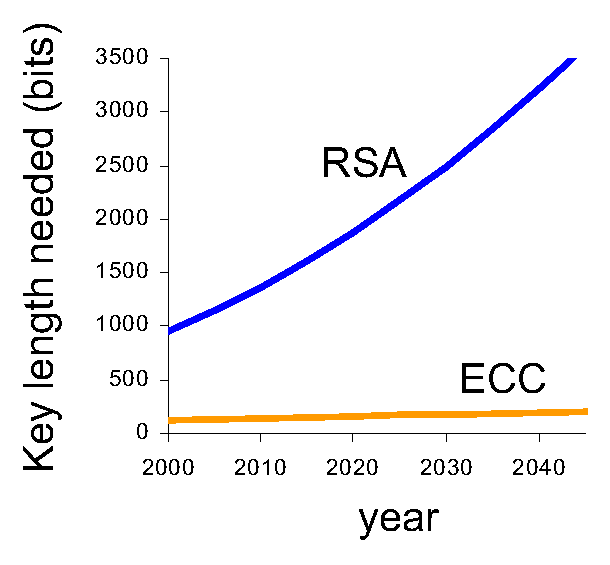
\includegraphics[scale=0.75]{figures/RSAKeylength}
\caption{Prognosis of the key lengths to be regarded safe for RSA and
  Elliptic Curves\vspace{1ex}} 
\label{RSAKeylength}
\end{center}
\end{figure}

In addition, a digital signature can be processed 10-times faster with ECC
than with RSA.  However, verification of a given signature is still more
efficient with RSA than with ECC. Refer to
figure~\ref{ThousandBitMultiplications} (source: Dr.~J.\ Merkle, Elliptic
Curve Cryptography Workshop, 2001) for a comparison.  The reason is that
RSA public keys can be chosen relatively small as long as the secret key is
sufficiently long.

% -> Figure 2
\begin{figure}[h]
\begin{center}
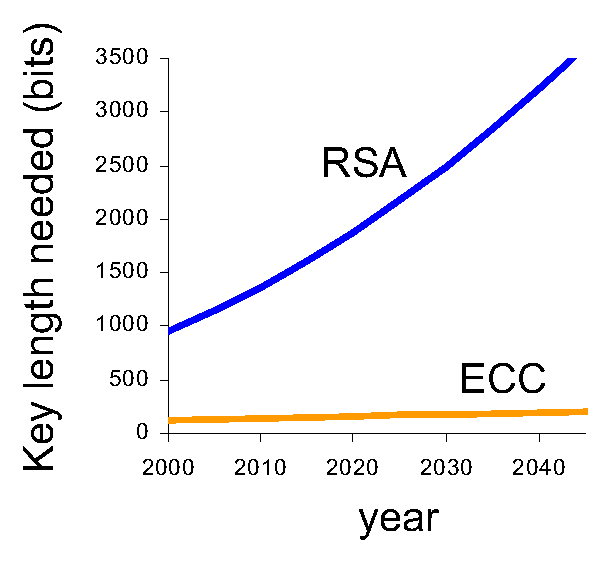
\includegraphics[scale=0.75]{figures/ThousandBitMultiplications}
\caption{Comparison of signing and verification time for RSA and Elliptic Curves} 
\label{ThousandBitMultiplications}
\end{center}
\end{figure}

Nevertheless, thin clients like smart cards usually have to store the (long) secret key
and have to process a digital signature rather than to verify one. Therefore, there is
a clear advantage for ECC in terms of efficiency.
\par
\smallskip
Today, the major problem with ECC-implementations is the lack of standardization.
There is only one way to implement RSA, but there are many ways for ECC: One can work with
different sets of numbers, different (elliptic) curves described by up to 6 parameters,
and a variety of representations of the elements on the curve. Each choice has its
advantages and disadvantages, and one can certainly construct the most efficient for
each application. However, this causes problems in interoperability. But if all
ECC-tools should be able to communicate with each other, they will have to support
all different algorithms, which might put the advantage of efficient computation and
the need of less storage capacity to the contrary.

Therefore, international standardization organizations like IEEE (P1363),
ASC (ANSI X9.62, X9.63), ISO/IEC as well as major players like RSA labs or
Certicom have recently started standardization initiatives. While the IEEE
only describes the different implementations, the ASC has explicitly stated
10 elliptic curves and recommends their usage. The advantage of the ASC
approach is that one needs only a single byte to indicate which curve is
meant. However, it is not clear yet whether the ASC-curves will become a de
facto standard.

Although we see no need to replace RSA in any application today, one should
take the usage of ECC-based tools into consideration whenever a new system
is set up --- in particular, when the tool should be available beyond 2005.


\subsection{Elliptic curves --- history}

Mathematicians have been researching elliptic curves for over 100 years. In the
course of time, many lengthy and mathematically complex results have been found
and published in connection with elliptic curves. A mathematician would say that
elliptic curves (or the mathematics behind them) are widely understood. This
research was originally purely mathematical. That is to say, elliptic curves
were investigated, for example, in the mathematical areas of number theory and
algebraic geometry, which are generally highly abstract. Even in the recent
past, elliptic curves played an important role in pure mathematics. In 1993 and
1994, Andrew Wiles\index{Wiles} published mathematical works that triggered enthusiasm far
beyond the specialist audience. In these works, he proved a conjecture put
forward in the 1960's. To put it short, this conjecture was concerned with the
connection between elliptic curves and what are called module forms. That which
is interesting for most people is that the works of Wiles also proved the famous
second theorem of Fermat. Mathematicians had spent centuries (Fermat lived from
1601 to 1665) trying to find a strict proof of this theorem. Understandably,
therefore, Wiles' proof got a good response. Fermat formulated his theorem as
follows (written in the border of a book):

\begin{quote} {\em
Cubum autem in duos cubos, aut quadratoquadratum in duos quadratoquadratos, et
generaliter nullam in infinitum ultra quadratum potestatem in duos ejusdem
nominis fas est dividere: cujus rei demonstrationem mirabilem sane detexi. Hanc
marginis exiguitas non caperet.
} \end{quote}

Translated freely, using the denotation of modern mathematics, this means: \\
No positive whole numbers $x, y$ and $z$ greater than zero exist such that $x^n +
y^n = z^n$ for $n>2$. I have found an amazing proof of this fact, but there is
too little space in the border [of the book] to write it down.

This is truly amazing: A statement that is relatively simple to understand (we
are referring to Fermat's second theorem here) could only be proved after such a
long period of time, although Fermat himself claimed to have found a proof.
What's more, the proof found by Wiles is extremely extensive (all of Wiles
publications connected with the proof made up a book in themselves). This should
therefore make it obvious that elliptic curves are generally based on highly
complex mathematics.

Enough about the role of elliptic curves in pure mathematics. In 1985 Neal
Koblitz and Victor Miller independently suggested using elliptic curves in
cryptography. Elliptic curves have thus also found a concrete practical
application. Another interesting field of application for elliptic curves is for
factorising whole numbers. (For example the RSA cryptography system is based on
the \index{Complexity} difficulty/complexity of finding prime factors of an
extremely large number.) In this area, procedures based on elliptic curves have
been investigated and partially used since 1987 (a study by H.W. Lenstra). There
are also prime number tests\index{Prime number!test} based on elliptic curves.

Elliptic curves are used differently in the various areas. Encryption procedures
based on elliptic curves are based on the difficulty of a problem known as
elliptic curve discrete logarithm\index{Logarithm problem!discrete}. The factorisation of whole numbers uses the
fact that a large number of elliptic curves can be generated for a natural
composite number $n$ with several prime factors; however, these curves are not
then groups for composite $n$. \hyperlink{faktell}{More information about this
can be found under Factorisation using elliptic curves.}

\subsection{Elliptic curves --- mathematical basics}

This section provides information about \index{Group} {\em groups} and
\index{Field} {\em fields}.

\subsubsection{Groups}

Because the term {\em group} is used differently in everyday language than in
mathematics, we will, for reasons of completeness, begin by introducing the
essential statement of the formal definition of a group:
\begin{itemize}
   \item A group is a non-empty set $G$ and an operation $+.$ The set $G$ is
closed under the operation $+.$ Regardless of which two elements $a, b$ from $G$
are taken, performing the operation on them gives an element in $G$ (i.e.
$a+b=c$, and $c$ lies in $G$).
   \item For all elements $a, b$ and $c$ in $G$: $(a+b)+c = a+(b+c)$.
   \item There exists an element $e$ in $G$ that behaves neutrally with respect
to the operation $+$. That means that for all a in the set $G: ~a+e = e+a = a.$
   \item For each element $a$ in $G$ there exists a so-called inverse element $-a$
($-a$ also lies in $G$) such that: $a+(-a) = (-a)+a = e$.
\end{itemize}
If also $a+b = b+a$ for all $a, b$ in $G$ then we call the group an {\em
Abelian} group. An operation denoted as $+$ indicates an {\em additive} group;
if the operation is denoted as $\cdot$, we speak of a {\em multiplicative}
group.

The simplest example of an (Abelian) group is the group of whole numbers under
the standard operation of addition. The set of whole numbers is denoted as
${\mathbb Z}$. ${\mathbb Z}$ has an infinite number of elements, because
${\mathbb Z} = \{ \cdots, -4, -3, -2, -1, 0, 1, 2, 3, 4, \cdots\}$. For example, the
operation of $1+2$ lies in ${\mathbb Z}$, for $1+2 = 3$ and $3$ lies in
${\mathbb Z}$. The neutral element in the group ${\mathbb Z}$ is $0$. The
inverse element of $3$ is $-3$, for $3+(-3) = 0$.

There are also {\em finite} groups. This means that these exists a set
$\mathcal{M}$ with a fixed number of elements and an operation $+$ such that the
above conditions are fulfilled. One example of this is any set ${\mathbb Z}_n$
where ${\mathbb Z}_n = \{0, 1, 2, 3, \cdots, n-1\}, n$ is a positive whole number
and the operation is addition mod $n$, i.e. $a$ and $b$ in ${\mathbb Z}_n$ are
subject to the operation $a+b \;{\rm mod~} n$.

\paragraph{Cyclic groups}
Cyclic groups\index{Group!cyclic} are those groups $G'$ that possess an element $g$
from which the group operation can be used to generate all other
elements in the group. This means that for each element $a$ in
$G'$ there exists a positive whole number $i$ such that if $g$ is
subject to the operation $i$ times (i.e. ``$g \cdot i$''),
$g+g+\cdots+g = a$ (additive group) or $g^i = g\cdot g \cdots g = a$
(multiplicative group). The element $g$ is the {\em generator} of
the cyclic group --- each element in $G�$ can be generated using
$g$ and the operation.

Now to the order of an element of the group: Let $a$ be in $G$. The smallest
positive whole number $r$ for which $a$ subject to the operation with itself $r$
times is the neutral element of the group $G�$ (i.e.: $r \cdot a = a+a+\cdots+a =
e$ bzw.\ $a^r = e$), is called the {\em order} of $a$.

The order of the group is the number of elements in the set $G$.

\subsubsection{Fields}

In mathematics, a field is understood to be a set $K$ with two operations
(denoted as $+$ and $\cdot$) which fulfils the following conditions:
\begin{itemize}
   \item The set $K$ forms an Abelian group together with the operation $+$
(addition), where $0$ is the neutral element of the operation $s$.
   \item The set $K$ (without the element 0) also forms an Abelian group
together with the operation $\cdot$ (multiplication).
   \item For all elements $a, b$ and $n$ in $K$, $n\cdot (a+b) = n \cdot a + n
\cdot b$ and $(a+b) \cdot n = a \cdot n + b \cdot n$.
\end{itemize}

There are {\em infinite} fields, i.e. the set on which the field is based
contains an infinite number of elements (e.g.: the field of real numbers). And
there are also finite fields, such as ${\mathbb Z}_p = \{0, 1, 2, 3, \cdots, p-1\}$
, where $p$ is a prime. ${\mathbb Z}_p$ with addition mod $p$ and multiplication
mod $p$ is a finite field.
\index{Field!Characteristic}
\paragraph{Characteristic of a field}
Let $K$ be a field and $1$ be the neutral element of $K$ with
respect to the multiplicative operation ``$\cdot$''. For positive
natural numbers $n$, let us understand $n_1$ to be $n_1 = 1 + 1 +
\cdots + 1$ ($n$ summands and $n_1$ is an element in $K$). If $n_1$
is then unequal to $0$ for all $n>0$, then we call $K$ a field
with characteristic zero. Otherwise, the characteristic of $K$ is
defined to be the smallest positive natural number $p$ for which
$p_1 = 0$ (note: $p$ is then a prime). Comment: The field of real
numbers has the characteristic $0$; the field ${\mathbb Z}_p$ has
the characteristic $p$.

\subsection{Elliptic curves in cryptography}

An elliptic curve is described by an equation. In order to keep it simple, we
restrict our explanation to elliptic curves over $${\mathbb Z}_p = \{0, 1, 2, 3,
\cdots, p-1\}$$ where $p$ is a prime greater than $3$. ${\mathbb Z}_p$ with
addition mod $p$ and multiplication mod $p$ is a finite field. However, we must
mention that elliptic curves can be defined over any (finite) field. In
particular, elliptic curves over fields with characteristic $2$ are extremely
interesting from a practical point of view because computers can be used to
represent the elements from these fields as bit strings. This leads to an
efficient implementation of the arithmetic in such fields, which means that a
computer can perform the operations of the field particularly quickly.

Because these points actually refer to the same thing, it is seldom necessary to distinguish between exact meanings.

An elliptic curve over ${\mathbb Z}_p$ is defined by an equation of the following form:
$$ y^2 \; ({\rm mod} \; p) = x^3 + ax + b ({\rm mod} \; p) $$
(thus: equality in the field ${\mathbb Z}_p$), where $a, b$ are in ${\mathbb Z}_p$ and $4a^3 + 27b^2$ mod $p$ is
not equal to zero. For fixed chosen numbers $a$ and $b$ in ${\mathbb Z}_p$, this equation has the pair of solutions
$$ {\bf E} = \left\{(x,y) \left| \begin{array}{c} x {\rm ~and~} y {\rm ~are~in~} {\mathbb Z}_p {\rm ~and~} \\
y^2  \equiv x^3 + ax + b \;({\rm mod~} p) {\rm ~and~} \\ 4a^3 + 27b^2 \not\equiv 0 \;
({\rm mod~} p)\end{array} \right. \right\}, $$ i.e. the set ${\bf E}$ consists of all pairs $x$ and $y$ that are a solution
(in ${\mathbb Z}_p$) of the above equation. It must be noted that the numbers $a, b$ and $p$ determine which pairs $(x,y)$
lie in the set ${\bf E}$. This means that $a, b$ and $p$ specify this set. The elements $(x,y)$ in ${\bf E}$ are called
points on the elliptic curve. In addition, ${\bf E}$ has one more element $O$ (the so-called point in infinity).
The set ${\bf E}$ is usually called an elliptic curve. 

We can now define an operation\footnote{A animated addition of elliptic curve points can be
found at the web page of Certicom\index{Certicom}:
\href{http://www.certicom.com/resources/ecc_tutorial/ecc_tutorial.html}{\tt http://www.certicom.com/resources/ecc\_tutorial/ecc\_tutorial.html}.}
(also denoted as $+$, although it is
not the standard/usual addition of real numbers) on two elements in ${\bf E}$ such that the operation delivers an element
that also lies in ${\bf E}$. The set ${\bf E}$ is therefore closed under the operation $+$. We can show
that ${\bf E}$ is a group. The neutral element of the group ${\bf E}$ is the point in infinity $O$. Thus, for every two
points $(x_1,y_1)$ and $(x_2,y_2)$ on the elliptic curve ${\bf E}$, there exists a point $(x_3,y_3)$ on ${\bf E}$ such that
the operation $+$ complies with the following: $(x_1,y_1) + (x_2,y_2) = (x_3,y_3)$. Under certain circumstances, these points
may also be equal to the point in infinity. Thus, when we speak of a point $P$ on an elliptic curve ${\bf E}$,
we mean that $P = (x,y)$ and $(x,y)$ lies in the set ${\bf E}$. Any two points on an elliptic curve specified by $a, b$ and $p$
can therefore be added and the result is a point that also lies on the same elliptic curve.

% \newpage
\begin{figure}[htbp]
\subsubsection*{Adding of two points on an elliptic curve}
The following two figures show an elliptic curve in the affine plane and
shows how points on an elliptic curve are added. Note that the point in infinity $O$ cannot be represented in
the affine plane.
\begin{center}
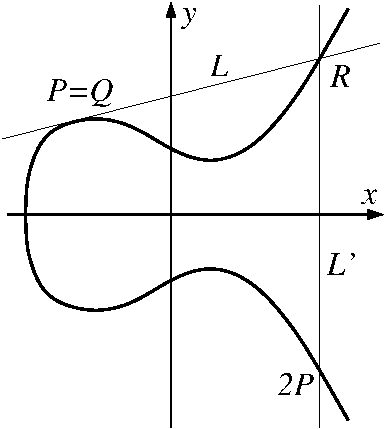
\includegraphics[scale=1.08]{figures/ec-mult2}
\caption{Doubling the point P} \vspace{\floatsep} \vskip +20 pt
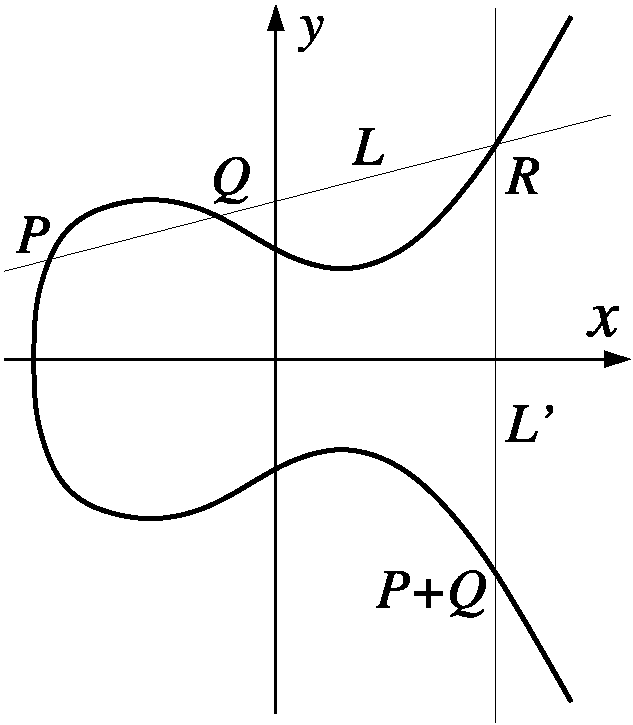
\includegraphics[scale=0.65]{figures/ec-add}
\caption{ Adding distinct points P and Q} % \footnotemark}
\end{center}
\end{figure}
% \addtocounter{footnote}{0}\footnotetext{The point $O$ cannot be represented in the affine plane.}
\enlargethispage{+20pt}

\newpage
We must note that ${\bf E}$ can have the following meanings:
\begin{itemize}
   \item the set ${\bf E}$ of solutions pairs $(x,y)$ for an equation including the point $O$
   \item the group ${\bf E}$ (with the operation ``addition of $(x_1,y_1)$ and $(x_2,y_2)$'')
   \item the elliptic curve ${\bf E}$ (which is actually the same as the group ${\bf E}$)
\end{itemize}
For cryptography, the important fact is that, for very large numbers, it appears to be extremely difficult to use a
given point $Q$ on an elliptic curve to determine which two points have to be added to obtain $Q$.

For large numbers $a, b$ and $p$ ($p$, for example, has a length of more than $160$ bits), the computer can easily add
the point $P$  $m$ times after another, i.e. to determine the point $P + P + \cdots + P = Q$ in an incredibly short space
of time (in a few fractions of a second) ($m$ summands $P$). Rather than $P + P + \cdots + P = Q$ ($m$ summands $P$)
we also write $mP = Q$. If we have a point $P$ and a point $Q$, which both lie on the same elliptic curve, no procedure
is known that enables us --- within an acceptable space of time --- to determine the number $m$ (assuming it actually exists)
for which $mP = Q$. This is referred to as the ``elliptic curve discrete logarithm problem'' (abbreviated to ECDLP)\index{ECDLP}.

We must note that not all elliptic curves are equally secure. This
means that we must choose the parameters $a$ and $b$ carefully
when defining a curve. For certain classes of elliptic curves, it
is possible to solve the ECDLP easier than in the general case.
Cryptographically unsuitable elliptic curves are called {\em abnormal}
curves (these are curves over ${\mathbb Z}_p$ for which the set
${\bf E}$ has precisely $p$ elements) and the {\em supersingular} curves
(the curves for which we can reduce the calculation of the ECDLP
to calculating the ``standard'' discrete logarithm in other finite
fields, i.e. simplify the calculation). There are therefore
cryptographically good and bad curves. However, for given
parameters $a$ and $b$ we can, with some difficulty, establish
whether or not the resulting elliptic curve is useful for
cryptographic purposes. The curves used in cryptography are
usually provided by experts. They ensure that the elliptic curves
they classify as secure satisfy the current security requirements.

For secure curves, the parameter $p$ determines how long it takes
to solve the ECDLP on this curve. The larger the parameter $p$,
the longer it takes to solve the problem. Experts recommend a bit
length of over $200$ bits for the parameter $p$. This makes it
clear why elliptic curves are so interesting for cryptography.
Because the parameter $p$ also determines the time required to
perform the signature/encryption procedure when using elliptic
curves in cryptography. The time taken to generate a pair of keys
also depends on $p$. Thus, small values (few bits) are desirable
here (in order to minimise the run times for the procedures);
however, the required security must still be maintained. For
example, with a length of $200$ bits for $p$, a {\em good}
elliptic curve is just as secure as an \index{RSA!module} RSA
module of over $1024$ bits in length (at least according to the
current state of research). The reason for this is that the
quickest algorithms for solving the {\em elliptic curve discrete
logarithm} problem have an exponential run time --- unlike the
sub-exponential run times that the best factorisation algorithms
currently have (number sieve, quadratic sieve or factorisation
with elliptic curves). Therefore, the parameters for cryptographic
procedures based on the problem of {\em factorising whole numbers}
must be greater than the parameters for cryptographic procedures
based on the ECDLP problem.

\subsubsection{Digital signatures using elliptic curves}

The {\em elliptic curve discrete logarithm problem} (ECDLP) \index{ECDLP} forms the basis for
elliptic-curve cryptography. Various signature procedures are based on this.
What they have in common is how they use the public parameters and how these
parameters are used to generate secret and public keys:
\begin{itemize}
    \item The parameters of the elliptic curve E, i.e. a prime number $p$ that
determines over which field ${\mathbb Z}_p$ the elliptic curve ${\bf E}$ is
defined, as well as the two numbers $a$ and $b$ in ${\mathbb Z}_p$.
    \item A point $G=(x,y)$ that lies on the elliptic curve ${\bf E}$.
    \item A prime number $r < p$ for which $rG=O$ (i.e. $G$ added $r$ times
gives the neutral element of the group ${\bf E}$) and $r$ is a factor of $\#{\bf
E}$ (where $\# {\bf E}$ is the number of elements in the set ${\bf E}$). The
point $G$ therefore has the order $r$ and is the generator of a cyclic subgroup
of ${\bf E}$ with the order $r$.
    \item The number $k = \#{\bf E}/r$ ($k$ is called the {\em cofactor}).
\end{itemize}
The parameters $a, b, p, G, r$ and $k$ listed above are called
{\em domain parameters}.\index{Domain parameters} They determine on which elliptic curve ${\bf
E}$ and in which cyclic subgroup of ${\bf E}$ a signature
procedure has been ``used''.

The secret key $s$ of the signature generator is a (random) whole number $s$ in
the interval $[1, r-1]$. The public key of the signature generator is a point
$W=(x,y)$ on the elliptic curve ${\bf E}$. The public key $W$ and secret key $s$
are interrelated as follows: $W = sG$. This means that the domain parameters
(particularly $G$) and the secret key $s$ are used to calculate the public key
$W$ (by adding $G$ $s$ times on ${\bf E}$). The ECDLP is obviously used here: If
$W$ and $G$ (as well as the other domain parameters used) are known, then it is
difficult to use these to calculate $s$. (If the parameters are chosen
correctly, this currently appears to be practically impossible).

In order to verify a signature, the recipient of the signature must know the
following:
\begin{enumerate}
   \item The signature procedure used,
   \item The hash function used,
   \item The domain parameters used to generate the signature
   \item The public key $W$ of the signature generator.
\end{enumerate}


\subsubsection{Factorisation using elliptic curves}

\hypertarget{faktell}{}

There are factorisation algorithms based on elliptic curves
\footnote{In 1987 H.W. Lenstra published
a factorisation algorithm, based on elliptic curves (see \cite{Lenstra1987}).
The biggest compound number currently factorised with elliptic curves is 
the number $ 628^{59}-1, $ which has 55 decimal digits. It was
found Oct. 6th, 2001 by M. Izumi 
(See \hyperlink{Lenstra2}{ECMNET}\index{ECMNET}).
}. 
More precisely, these procedures exploit the fact that elliptic curves can
be defined over ${\mathbb Z}_n$ ($n$ composite number). Elliptic curves 
over ${\mathbb Z}_n$ do not form a group, because not every point on such 
an elliptic curve has an inverse point. This is connected with the fact 
that - if $n$ is a composite
number - there exist elements in ${\mathbb Z}_n$ that do not have an inverse
with respect to multiplication mod $n$. In order to add two points on an
elliptic curve over ${\mathbb Z}_n$, we can calculate in the same way as on
elliptic curves over ${\mathbb Z}_p$. Addition of two points (on an elliptic
curve over ${\mathbb Z}_n$), however, fails if and only if a factor of $n$ has
been found. The reason for this is that the procedure for adding points on
elliptic curves gives elements in ${\mathbb Z}_n$ and calculates the inverse
elements for these (with respect to multiplication mod $n$) in ${\mathbb Z}_n$.
The extended \index{Euclidean algorithm} Euclidean algorithm is used here. If
the addition of two points (that lie of an elliptic curve over ${\mathbb Z}_n$)
gives an element in ${\mathbb Z}_n$ that does not have an inverse element in
${\mathbb Z}_n$, then the extended Euclidean algorithm delivers a genuine factor
of $n$.

Factorisation using elliptic curves thus principally works as follows: You
select random curves over ${\mathbb Z}_n$, as well as random points (that lie on
this curve) and add them; you thus obtain points that also lie on the curve or
find a factor of $n$. Factorisation algorithms based on elliptic curves
therefore work probabilistically. The opportunity of defining large number of
elliptic curves over ${\mathbb Z}_n$ allows you to increase the probability of
finding two points which you can add to obtain a factor of $n$. These procedures
are therefore highly suitable for parallelisation.

\subsection{Implementing elliptic curves}

CrypTool\index{CrypTool} uses elliptic curves for the digital signature function.

It implements the basic algorithms for group operations, for generating elliptic
curves, for importing and exporting parameters for elliptic curves over finite
fields with $p$ ($p$ prime) elements. The algorithms have been implemented in
ANSI C and comply with draft no. 8 of the IEEE P1363 work group {\em Standard
Specifications for Public Key Cryptography}

{\href{http://grouper.ieee.org/groups/1363}{\tt
http://grouper.ieee.org/groups/1363}}.

The procedure implements the cryptographic primitives for generating and
verifying signatures for the variations of Nyberg-Rueppel signatures and
\index{DSA} DAS signatures based on elliptic curves (in accordance with draft
no. 8 of the IEEE P1363 work group). This was done in collaboration with the
Secude GmbH --- using the above library and the Secude SDK.
\index{Secude}

\newpage
%\addcontentsline{toc}{subsection}{Literaturverzeichnis}
\begin{thebibliography}{99999}
\addcontentsline{toc}{subsection}{Bibliography}
        \bibitem[Lenstra1987]{Lenstra1987} H.W. Lenstra\\ \index{Lenstra 1987}
                Factoring integers with elliptic curves, Annals of Mathematics 126, pp. 649-673, 1987.
\end{thebibliography}
%\newpage

\section*{Web links}\addcontentsline{toc}{subsection}{Web links}

\begin{enumerate}
   \item Certicom Online Tutorial, \index{Certicom}\\
                \href{http://www.certicom.com/resources/ecc_tutorial/ecc_tutorial.html}{\texttt{http://www.certicom.com/resources/ecc\_tutorial/ecc\_tutorial.html}}
        \item IEEE P1363

                \href{http://grouper.ieee.org/groups/1363}{\texttt{http://grouper.ieee.org/groups/1363}}
        \item  \hypertarget{Lenstra2}{}
An informative web page about factorisation with elliptic curves.

\href{http://www.loria.fr/~zimmerma/records/ecmnet.html}{\texttt{http://www.loria.fr/\~{}zimmerma/records/ecmnet.html}}

There, one finds literature to the topic factorisation with elliptic curves as well as links to other web page. 

\end{enumerate}


% Local Variables:
% TeX-master: "../script-en.tex"
% End:

\renewcommand{\CTBChapName}{(Chap BitCiphers)}    % $Id: cryptomethods.tex 3712 2016-03-22 23:36:46Z xesslinger $
% !Mode:: "TeX:DE"    % Setting document mode and submode for WinEdt
% ..............................................................................
% B i t b l o c k -  u n d  B i t s t r o m - V e r s c h l � s s e l u n g
% ~~~~~~~~~~~~~~~~~~~~~~~~~~~~~~~~~~~~~~~~~~~~~~~~~~~~~~~~~~~~~~~~~~~~~~~~~~~~~~

\begin{bibunit}[babalpha] %% alpha: Chapter bibliography shows authors abbreviation


%BERM0 Changed when bc becoming part of the CT book.
%BERM1 Transformed to comment when bc becoming part of the CT book: There it already was in script-en.tex.
%BERM2 Transformed to comment when bc becoming part of the CT book: Added there to script-en.tex.
%BERM3 Redefined new commands already existing in moderncryptography.tex when bc becoming part of the CT book
%BERM3 (see http://tex.stackexchange.com/questions/36175/what-do-newcommand-renewcommand-and-providecommand-do-and-how-do-they-differ).

%BERM1 \documentclass[11pt,a4paper,leqno]{report}
%BERM1 \usepackage[latin1]{inputenc}
%BERM1 \usepackage[T1]{fontenc}
%BERM1 \usepackage{german}
%BERM1 \usepackage{amsmath,amssymb,amscd,latexsym}
%BERM1 \usepackage{color}
%BERM1 \usepackage{hyperref}
%BERM1 \usepackage{makeidx}
%BERM1 \usepackage[pdftex]{graphicx}
%BERM1 \usepackage{float}

% ++++++++++++++++++++++++++++++++++++++++++++++++++++++++++++++++++++++++++
% Pommerenings Spezialit�ten
% ~~~~~~~~~~~~~~~~~~~~~~~~~~~~~~~~~~~~~~~~~~~~~~~~~~~~~~~~~~~~~~~~~~~~~~~~~~
\newcommand*{\F}{\mathbb{F}}
\newcommand*{\M}{\mathbb{M}}

%% yyyyyyyyycccc 3.8.16 Side effect of using \begin{bibunit} with 5 renews: The commands
%% are no more known from before and so cannot be renewed (so still to be newly defined)
%% \renewcommand*{\C}{\mathbb{C}}   %BERM3
%% \renewcommand*{\N}{\mathbb{N}}   %BERM3
%% \renewcommand*{\Q}{\mathbb{Q}}   %BERM3
%% \renewcommand*{\R}{\mathbb{R}}   %BERM3
%% \renewcommand*{\Z}{\mathbb{Z}}   %BERM3
\newcommand*{\C}{\mathbb{C}}
\newcommand*{\N}{\mathbb{N}}
\newcommand*{\Q}{\mathbb{Q}}
\newcommand*{\R}{\mathbb{R}}
\newcommand*{\Z}{\mathbb{Z}}

\newcommand*{\lsb}{\operatorname{lsb}}
\newcommand*{\Oh}{\operatorname{O}}

% ++++++++++++++++++++++++++++++++++++++++++++++++++++++++++++++++++++++++++
% CrypTool-Spezialit�ten
% ~~~~~~~~~~~~~~~~~~~~~~~~~~~~~~~~~~~~~~~~~~~~~~~~~~~~~~~~~~~~~~~~~~~~~~~~~~
%BERM1 \newtheorem{definition}{Definition}[section]
%BERM1 \newtheorem{satz}{Satz}[section]
%BERM1 \newenvironment{Beweis}[1]{\noindent\textbf{Beweis #1} \\}{\hfill$\Box$\par}
%BERM1 \newenvironment{example}[1]{\noindent\textbf{Beispiel#1}}{}
%BERM1 \newenvironment{remark}[1]{\noindent\textbf{Bemerkung#1}}{}
%BERM1 \setcounter{secnumdepth}{4} % Nummerierung auch bei subsubsection
%BERM1 \floatstyle{ruled}
%BERM1 \newfloat{sagecode}{!ht}{loc}[chapter]
%BERM1 \floatname{sagecode}{SageMath-Beispiel}

\sloppy
\frenchspacing
%BERM1 \makeindex
%BERM1 \begin{document}

%BERM0 \setcounter{chapter}{98}  % ====> Dummy - beim Einf�gen ins CT-Skript l�schen <=====
\setcounter{satz}{0}
\setcounter{definition}{0}


\newpage %BERM0
\hypertarget{Chapter_BitCiphers}{}   %BERM0
\chapter{Einf�hrung in die Bitblock- und Bitstrom-Verschl�sselung}
\label{Chapter_BitCiphers}
(\hyperlink{author_Klaus-Pommerening}{Klaus Pommerening},
 Januar--Juni 2015; Updates: Jan. 2016, Apr. 2016) \\

\noindent
W�hrend asymmetrische Verschl�sselung meistens zahlentheoretische Methoden
verwendet, beruhen die heutigen symmetrischen
Verschl�sselungsverfahren\index{Verschl�sselung!symmetrisch}
in der Regel auf Boolescher Algebra\index{Boolesche Algebra}\index{Algebra!Boolesche},
d.\,h., auf Manipulationen von Bits.
Das ist eine ganz andere Art von Mathematik, f�r Einsteiger vielleicht
ungewohnt, so dass dieses Kapitel eine sanfte Einf�hrung in dieses mathematische
Gebiet sein soll. Vorkenntnisse aus einem Grundkurs Mathematik am Gymnasium
sollen ausreichen. Ohne weitere Erkl�rung als bekannt
angenommen werden die Begriffe "`Variable"' und "`Funktion"', auch f�r Argumente
und Werte in anderen Mengen als den reellen Zahlen.

Beginnen wir also mit der Beschreibung, wie Bits interpretiert, verkn�pft
und durch Funktionen, sogenannte Boolesche
Funktionen\index{Boolesche Funktion}\index{Funktion!Boolesche}, verarbeitet werden.
Namenspatron dieses Fachgebiets ist
George Boole\index{Boole, George}\footnote{%
  George Boole, englischer Mathematiker, Logiker und Philosoph,
  2.11.1815--8.12.1864.
},
der durch die Einf�hrung der elementaren logischen Operationen die Logik
mathematisch formalisierte ("`Logikkalk�l\index{Logikkalk�l}"').
Moderne symmetrische Verschl�sselungsverfahren, wie auch
Hash-Funktionen\index{Hashfunktion},
werden durch Systeme von Booleschen Funktionen beschrieben.

Der Schwerpunkt dieses Kapitels liegt in der Einf�hrung in die
mathematischen Grundlagen der Verschl�sselungstechniken, die auf
Bits operieren. Konkrete Verfahren werden nicht detailliert beschrieben;
hierf�r sei auf die B�cher von
Menezes/Orschot/Vanstone \cite{Menezes2001},
Oppliger \cite{Oppliger2011},
Paar und Pelzl \cite{PaPe2009},
Schmeh \cite{Schm2003, Schm2016}
und Stamp \cite{Stamp2007} verwiesen.

Noch ein Wort zur Nomenklatur: Die Verfahren werden in der Literatur
meist als "`Blockchiffren\index{Blockchiffre}"' oder
"`Stromchiffren\index{Stromchiffre}"' bezeichnet, ohne
das Pr�fix "`Bit-"'. Das ist manchmal missverst�ndlich, da -- besonders
bei Stromchiffren -- auch andere Zeichens�tze (Alphabete, Buchstaben)
als kleinste Einheiten verwendet werden. Der Deutlichkeit halber
sollte man im Zweifelsfall also die "`Bits"' mit in die Bezeichnung
aufnehmen.

Das Thema dieses Kapitels ist also mit anderen Worten

%\begin{quote}
   {\bf Symmetrische Verschl�sselung von mit Bits dargestellten Informationen}.
%\end{quote}

\noindent Die mathematischen Grundlagen und Methoden geh�ren zu den Gebieten

   {\bf Boolesche Algebra\index{Boolesche Algebra}\index{Algebra!Boolesche}
   und endliche K�rper\index{endlicher K�rper}\index{K�rper!endlich}}.


% ++++++++++++++++++++++++++++++++++++++++++++++++++++++++++++++++++++++++++
\newpage
\section{Boolesche Funktionen}\label{s-bool-fct}
\subsection{Bits und ihre Verkn�pfung}\label{s-bool-bit}

Die Objekte, mit denen Computer auf der untersten Software-Ebene operieren,
sind Bits\index{Bit} oder Gruppen von Bits (z.\,B. Bytes\index{Byte},
die meist aus 8 Bits bestehen,
oder "`W�rter\index{Wort}"', je nach Computer-Architektur meist 32 oder 64 Bits).
Der Umgang mit den Bits $0$ und $1$ und mit den elementaren
logischen Operationen wie "`und"' (AND), "`oder"' (OR),
"`nicht"' (NOT) und "`exklusives oder"' (XOR) ist zwar den meisten
vertraut, soll aber hier kurz beschrieben werden, auch um die verwendete
Terminologie einzuf�hren.

Bits k�nnen logisch interpretiert werden als die
Wahrheitswerte\index{Wahrheitswert} "`wahr"'
(True, T) und "`falsch"' (False, F). Sie k�nnen auch algebraisch interpretiert
werden als die Werte $0$ (entspricht F) und $1$ (entspricht T). Mathematisch
gesprochen sind sie dann Elemente der zweielementigen Menge $\{0, 1\}$,
die wir hinfort in diesem Kapitel mit $\F_2$ bezeichnen werden; warum,
wird gleich erkl�rt:

Betrachtet man n�mlich den Restklassenring von $\Z$ modulo $2$, so
hat dieser zwei Elemente und ist ein K�rper\index{K�rper},
da $2$ eine Primzahl ist. Die Addition in diesem K�rper
entspricht genau der logischen Verkn�pfung XOR\index{XOR},
die Multiplikation der logischen Verkn�pfung AND\index{AND},
wie man in Tabelle~\ref{t-bool-xor} sieht. Tabelle~\ref{t-bool-trf}
listet die Umrechnungsformeln zwischen den elementaren logischen
und algebraischen Operationen auf.

\begin{table}[h]
\begin{center}
\begin{tabular}{|cc|ccc||cc|cc|} \hline
   \multicolumn{5}{|c||}{\bf logisch} & \multicolumn{4}{c|}{\bf algebraisch} \\ \hline
   \multicolumn{2}{|c|}{Bits} & \multicolumn{3}{|c||}{Verkn�pfung} &
        \multicolumn{2}{|c|}{Bits} & \multicolumn{2}{|c|}{Verkn�pfung} \\ \hline
   $x$ & $y$ & OR & AND & XOR & $x$ & $y$ & + & $\cdot$ \\ \hline
    F  &  F  & F  &  F  &  F  &  0  &  0  &  0  &  0    \\
    F  &  T  & T  &  F  &  T  &  0  &  1  &  1  &  0    \\
    T  &  F  & T  &  F  &  T  &  1  &  0  &  1  &  0    \\
    T  &  T  & T  &  T  &  F  &  1  &  1  &  0  &  1    \\
   \hline
\end{tabular}
\end{center}
\caption{Die wichtigsten Verkn�pfungen von Bits\index{Bit}. Dabei ist das logische
  XOR\index{XOR} identisch mit dem algebraischen +, das logische AND\index{AND} mit dem
  algebraischen $\cdot$ (Multiplikation).}\label{t-bool-xor}
\end{table}

\begin{table}[h]
\begin{center}
\begin{tabular}{|rcl|} \hline
   \multicolumn{3}{|c|}{\bf algebraisch nach logisch}          \\ \hline
   $x + y$      & = & $(x \vee y) \wedge (\neg x \vee \neg y)$ \\
   $x \cdot y$  & = & $x \wedge y$                             \\ \hline \hline
   \multicolumn{3}{|c|}{\bf logisch nach algebraisch}          \\ \hline
   $x \vee y$   & = & $x + y + x\cdot y$                       \\
   $x \wedge y$ & = & $x \cdot y$                              \\
   $\neg x$     & = & $1 + x$                                  \\ \hline
\end{tabular}
\end{center}
\caption{Umrechnung der algebraischen Operationen in logische und umgekehrt}\label{t-bool-trf}
\end{table}

Da die algebraische Struktur als K�rper\index{K�rper} f�r die Kryptographie
eine herausragende Rolle spielt, wird hier die in der Algebra �bliche
Bezeichnung f�r endliche K�rper\index{K�rper!endlich} $\F_q$ (oft
auch $\text{GF}(q)$ f�r "`Galois\index{Galois, �variste}\footnote{%
  �variste Galois, franz�sischer Mathematiker,
  25.10.1811--31.5.1832.
}
Field"', dabei ist $q$ die Anzahl der Elemente) �bernommen\footnote{%
  Auch SageMath verwendet die Bezeichnung $\text{GF}(q)$.
}.
In diesem Kontext ist es sinnvoll, f�r die
Verkn�pfungen die algebraischen Symbole $+$ (f�r XOR) und
$\cdot$ (f�r AND) zu verwenden, wobei der Multiplikationspunkt wie
auch sonst in der Mathematik oft weggelassen wird. Kryptographen benutzen
gerne auch die Symbole $\oplus$ und $\otimes$, die allerdings in der
Mathematik mit ganz anderen Bedeutungen\footnote{%
  direkte Summe und Tensorprodukt von Vektorr�umen
}
belegt sind und daher in diesem Text -- abgesehen von Diagrammen --
meist vermieden werden.

Zur Verdeutlichung sei noch explizit auf einige Besonderheiten des
algebraischen Rechnens im bin�ren Fall (d.\,h., in Charakteristik $2$)
hingewiesen:
\begin{itemize}
   \item In einer Summe heben sich zwei gleiche Summanden gegenseitig
      weg, d.\,h., sie ergeben zusammen $0$. Allgemeine Regel: $x + x = 0$
      oder $2x = 0$.
   \item Allgemeiner ergibt eine gerade Anzahl gleicher Summanden immer $0$,
      w�hrend eine ungerade Anzahl gleicher Summanden genau diesen Summanden
      ergibt. Allgemeine Regel:
\[
         m \, x := \underbrace{x + \cdots + x}_m \quad = \quad
            \begin{cases}
               0 & \text{f�r gerades } m \\ x & \text{f�r ungerades } m.
            \end{cases}
\]
   \item Bei algebraischen Umformungen ist eine Subtraktion dasselbe wie
      eine Addition; man kann Plus- und Minuszeichen beliebig gegeneinander
      austauschen. Allgemeine Regel: $x + y = x - y$.
   \item Alle drei binomischen Formeln, also f�r $(x + y)^2$, $(x - y)^2$,
      $(x + y)(x - y)$, fallen zu einer einzigen zusammen:
\[
         (x + y)^2 = x^2 + y^2.
\]
      Denn das doppelte Produkt ist $0$.
\end{itemize}


\subsection{Beschreibung Boolescher Funktionen}\label{ss-bool-descr}

Definieren wir zun�chst ganz naiv: Eine {\bf Boolesche
Funktion}\index{Boolesche Funktion}\index{Funktion!Boolesche} ist eine
Vorschrift (oder eine Rechenregel oder ein Algorithmus), die aus einer
bestimmten Anzahl von Bits ein neues Bit erzeugt. Bevor wir diese
Definition mathematisch pr�zise fassen (siehe Definition~\ref{def-bool-fkt}),
soll sie zun�chst etwas anschaulicher gemacht werden.

F�r eine vertiefte Darstellung sei auf \cite{CuSt2009} oder \cite{Pomm2008, Pomm2014}
sowie die beiden Artikel von Claude Carlet\footnote{%
  siehe auch dessen Publikationsverzeichnis unter
  %BERM \url statt \href
  % \href{http://www.math.univ-paris13.fr/~carlet/pubs.html}{\tt http://www.math.univ-paris13.fr/$\sim$carlet/pubs.html}
  \url{http://www.math.univ-paris13.fr/~carlet/pubs.html}
} in \cite{CrHa2010}\footnote{%
  online zu finden unter
  \url{http://www.math.univ-paris13.fr/~carlet/chap-fcts-Bool-corr.pdf}  und
  \url{http://www.math.univ-paris13.fr/~carlet/chap-vectorial-fcts-corr.pdf}
} verwiesen.

Als ganz einfaches Musterbeispiel dient die Funktion AND\index{AND}: Sie nimmt zwei Bits
entgegen und erzeugt daraus ein neues Bit nach der bekannten Verkn�pfungsregel
des logischen "`und"', siehe Tabelle~\ref{t-bool-xor}.

Als etwas komplizierteres Beispiel m�ge die Funktion $f_0$ dienen, die aus drei Bits
$x_1$, $x_2$ und $x_3$ den Wert
\begin{equation}\label{bc_sample-fct-f0-with-3-vars}
   f_0(x_1, x_2, x_3) = x_1\: \text{AND}\: (x_2\: \text{OR}\: x_3)
\end{equation}
% Hier equation statt  \[...\]  oder  $$...$$, die wohl �qivalent sind. Vorher war:
%  \[
%     f_0(x_1, x_2, x_3) = x_1\: \text{AND}\: (x_2\: \text{OR}\: x_3)
%  \]
berechnet.

Veranschaulichen kann man sich eine Boolesche Funktion durch eine
"`Black Box\index{Black Box}"':
\begin{center}
\begin{picture}(140,60)
   \put(20,25){\colorbox{black}{XgXXXXXXXXXX}}
%   \put(20,20){\framebox(100,20){$f$}}
   \put(25,35){\line(0,1){10}}
   \put(35,35){\line(0,1){10}}
   \put(45,35){\line(0,1){10}}
   \put(65,40){\ldots}
   \put(95,35){\line(0,1){10}}
   \put(105,35){\line(0,1){10}}
   \put(115,35){\line(0,1){10}}
   \put(70,20){\line(0,-1){10}}
   \put(48,50){\sf Input-Bits}
   \put(48,0){\sf Output-Bit}
\end{picture}
\end{center}

\noindent Was innerhalb dieser "`Black Box"' passiert, kann man auf verschiedene
Arten beschreiben:
\begin{itemize}
   \item {\bf mathematisch} durch eine Formel,
   \item {\bf informatisch} durch einen Algorithmus,
   \item {\bf technisch} durch ein Schaltnetz\index{Schaltnetz}
      (oder Schaltdiagramm),
   \item {\bf pragmatisch} durch eine Wahrheitstafel\index{Wahrheitstafel}
      (das ist die Wertetabelle).
\end{itemize}
Die Beispielfunktion $f_0$ ist mathematisch definiert in der
Gleichung~(\ref{bc_sample-fct-f0-with-3-vars}). Der entsprechende Algorithmus
wird hier am besten ebenfalls durch diese Formel beschrieben, da keinerlei
Verzweigungen oder bedingte Anweisungen n�tig sind. Als Schaltnetz kann man
$f_0$ etwa wie in Abbildung~\ref{fig-bool-circuit} visualisieren.
Die Wahrheitstafel gibt zu jedem Input-Tripel einfach den Wert von $f_0$ an,
siehe Tabelle~\ref{tab-bool-wt}.

\begin{figure}[h]
\begin{center}
\begin{picture}(130,90)
   \put(58,30){AND}
   \put(70,29){\vector(0,-1){20}}
   \put(45,0){$f_0(x_1,x_2,x_3)$}
   \put(22,80){$x_1$}
   \put(67,80){$x_2$}
   \put(109,80){$x_3$}
   \put(88,55){OR}
   \put(90,51){\vector(-1,-1){10}}
   \put(110,75){\vector(-1,-1){10}}
   \put(78,75){\vector(1,-1){10}}
   \put(30,75){\vector(1,-1){34}}
\end{picture}
\end{center}
\caption{Beispiel eines Schaltnetzes}\label{fig-bool-circuit}
\end{figure}

\begin{table}[hbpt]
\begin{center}
\begin{tabular}{|ccc|c|} \hline
   $x_1$ & $x_2$ & $x_3$ & $f_0(x_1,x_2,x_3)$ \\ \hline
      0  &   0   &   0   &  0  \\
      0  &   0   &   1   &  0  \\
      0  &   1   &   0   &  0  \\
      0  &   1   &   1   &  0  \\
      1  &   0   &   0   &  0  \\
      1  &   0   &   1   &  1  \\
      1  &   1   &   0   &  1  \\
      1  &   1   &   1   &  1  \\
   \hline
\end{tabular}
\end{center}
\caption{Beispiel einer Wahrheitstafel}\label{tab-bool-wt}
\end{table}

Die Bezeichnung "`Wahrheitstafel\index{Wahrheitstafel}"' kommt von der Interpretation der
Bits im Logikkalk�l\index{Logikkalk�l}: 0 (= F) bedeutet "`falsch"', 1 (= T) bedeutet "`wahr"'.
Der Wert $f(x_1,\ldots,x_n)$ einer Booleschen Funktion $f$ sagt dann,
ob der gesamte Ausdruck wahr oder falsch ist, wenn die einzelnen Input-Bits
$x_1,\ldots,x_n$ die angegebenen Wahrheitswerte haben.

Die Verbindung zur Technik, also die Beziehung zwischen Logikkalk�l
und elektrischen Schaltungen, wurde im Wesentlichen von
Shannon\index{Shannon, Claude}\footnote{%
  Claude Elwood Shannon, amerikanischer Mathematiker und Elektrotechniker,
  30.4.1916--24.2.2001.
}
entwickelt.

\subsection{Die Anzahl Boolescher Funktionen}\label{ss-bool-enum}

Die obige Wahrheitstafel f�r $f_0$ suggeriert eine einfache Abz�hlung aller
Booleschen Funktionen:
Bei drei Variablen gibt es $8 = 2^3$ verschiedene Input-Tripel, denn jedes
einzelne Input-Bit kann unabh�ngig von den beiden anderen Bits die Werte $0$ oder $1$
annehmen. Eine Boolesche Funktion $f$ wiederum kann f�r jedes Input-Tripel
unabh�ngig von den sieben anderen Tripeln $0$ oder $1$ werden, das
sind $8$ unabh�ngige M�glichkeiten f�r $0$ oder $1$, also insgesamt $2^8$.
Also gibt es $256 = 2^8$ Boolesche Funktionen von drei Variablen.

Im allgemeinen Fall haben wir $N = 2^n$ verschiedene Besetzungen f�r
die $n$ Input-Variablen, und f�r jeden dieser $N$ Inputs kann die
Funktion $0$ oder $1$ werden, das macht $2^N$ verschiedene
M�glichkeiten. Die allgemeine Formel ist also:

\begin{satz}\label{thm-bool-enum}
   Es gibt genau $2^{2^n}$ verschiedene Boolesche Funktionen von
   $n$ Variablen.
\end{satz}

Bei vier Variablen sind das schon $2^{16} = 65536$ St�ck, und die Formel
sagt, dass die Anzahl superexponenziell\index{superexponenziell} anw�chst: Der Exponent w�chst
ja selbst schon exponenziell.

Alle 16 Booleschen Funktionen von zwei Variablen sind im
Abschnitt~\ref{ss-bool-2}, Tabelle~\ref{tab-bool-2}, aufgelistet.

\subsection{Bitbl�cke und Boolesche Funktionen}\label{ss-bool-blck}

F�r Gruppierungen von Bits gibt es je nach Kontext verschiedene
Bezeichnungen\footnote{%
   Begrifflich beschreiben sie das gleiche. In Python\index{Python} bzw. SageMath
   entsprechen den verschiedenen Bezeichnungen aber z.\,T. unterschiedliche
   Typen.
}:
Vektoren\index{Vektor}, Listen\index{Liste}, ($n$-) Tupel\index{Tupel},
\ldots, bei bestimmten Gr��en auch spezielle Bezeichnungen wie Bytes\index{Byte}
(f�r 8 Bits), W�rter\index{Wort} (f�r 32 oder
64 Bytes, je nach Prozessorarchitektur) \ldots\
In diesem Kapitel wird �berwiegend
die in der Kryptographie g�ngige Bezeichnung "`Bitbl�cke\index{Bitblock}"' verwendet.
Ein {\bf Bitblock} der L�nge $n$ ist also eine Liste $(x_1, \ldots, x_n)$ von
Bits. Hierbei kommt es auf die Reihenfolge an. Es gibt acht
verschiedene Bitbl�cke der L�nge $3$. Dies sind sie:
\[
   (0,0,0), (0,0,1), (0,1,0), (0,1,1), (1,0,0), (1,0,1), (1,1,0), (1,1,1).
\]
Gelegentlich werden sie, wenn dadurch kein Missverst�ndnis zu bef�rchten ist, auch
ohne Klammern und Kommas als Bitketten\index{Bitkette} geschrieben\footnote{%
   Manchmal werden sie auch in Spaltenform, als $n \times 1$-Matrizen,
   geschrieben, wenn die Interpretation als Vektor\index{Vektor} im Vordergrund steht.
}:
\[
   000, 001, 010, 011, 100, 101, 110, 111.
\]

Oft wird die abgek�rzte Schreibweise $x$ f�r $(x_1, \ldots, x_n)$ verwendet,
die ausdr�ckt, dass
Bitbl�cke\index{Bitblock} Objekte "`eigenen Rechts"' sind. Die $2^n$ verschiedenen
Bitbl�cke der L�nge $n$ sind genau die Elemente des kartesischen Produkts
$\F_2^n = \F_2 \times \cdots \times \F_2$. Dieses kartesische Produkt
hat eine "`nat�rliche"' Vektorraum-Struktur\index{Vektorraum} -- man kann Bitbl�cke
$x$ und $y \in \F_2^n$ addieren und mit Skalaren $a \in \F_2$ multiplizieren:
\[
   (x_1, \ldots, x_n) + (y_1, \ldots, y_n) =  (x_1 + y_1, \ldots, x_n + y_n),
\]
\[
   a \cdot (x_1, \ldots, x_n) = (a \cdot x_1, \ldots, a \cdot x_n).
\]

Damit k�nnen wir nun die mathematisch exakte Definition formulieren:

\begin{definition}\label{def-bool-fkt}\index{Boolesche Funktion}\index{Funktion!Boolesche}
  Eine {\bf Boolesche Funktion von $n$ Variablen} ist eine Abbildung
\[
     f\!\!: \F_2^n \longrightarrow \F_2.
\]
\end{definition}
Eine solche nimmt als Argument also einen Bitblock\index{Bitblock} der L�nge $n$
und produziert daraus ein Bit.

Die Menge aller Booleschen Funktionen auf $\F_2^n$ wird im Folgenden gelegentlich
mit $\mathcal{F}_n$ bezeichnet. Nach Satz~\ref{thm-bool-enum} hat sie
$2^{2^n}$ Elemente.

\begin{description}
   \item[Konvention:] Beschreibt man eine Boolesche Funktion durch ihre
      Wahrheitstafel, so ordnet man diese, wie auch oben im Beispiel
      schon gesehen, in der Regel lexikographisch\index{lexikographisch}\footnote{%
        Bei einer lexikographischen Ordnung\index{Ordnung!lexikographisch}
        werden die zu ordnenden
        Zeichenketten (wie in einem Lexikon) nach der Gr��e des ersten
        Zeichens -- hier $0$ oder $1$ mit $0 < 1$ -- geordnet.
        Falls dieses gleich ist, nach der Ordnung des zweiten Zeichens
        usw. Lexikographisch geordnet ist die Folge $011,100,101$. Nicht
        lexikographisch geordnet die Folge $100,101,011$, weil hier die
        dritte Zeichenkette mit einer $0$ beginnt, die kleiner ist als das
        Anfangszeichen der davor stehenden Zeichenkette. Die zu Beginn
        von \ref{ss-bool-blck} aufgeschriebene Reihenfolge der acht
        Bitbl�cke der L�nge $3$ folgt der lexikographischen Ordnung.
      } nach $x \in \F_2^n$;
      diese Ordnung ist, anders ausgedr�ckt, die nat�rliche Ordnung der
      Zahlen $a = 0, \ldots, 2^n-1$, wenn diese bin�r als
\[
     a = x_1\cdot 2^{n-1} + \cdots + x_{n-1}\cdot 2 + x_n
\]
      dargestellt und auf diese Weise den Bitbl�cken\index{Bitblock}
      $(x_1,\ldots,x_n) \in \F_2^n$ zugeordnet werden.
\end{description}

\subsection{Logische Ausdr�cke und disjunktive Normalform}\label{ss-bool-dnf}

F�r die mathematische Beschreibung Boolescher Funktionen, also wie
oben gesagt die Beschreibung durch eine Formel, sind im wesentlichen
au�er der Wahrheitstafel zwei Ans�tze gebr�uchlich:
\begin{itemize}
   \item In der Logik werden Boolesche Funktionen durch Disjunktionen\index{Disjunktion}
      (die Operation OR\index{OR}, auch $\vee$ geschrieben), Konjunktionen\index{Konjunktion}
      (die Operation AND\index{AND}, auch $\wedge$ geschrieben) und Negationen
      (die Operation NOT\index{NOT}, auch $\neg$ geschrieben) ausgedr�ckt.
      Zusammensetzungen dieser Operationen hei�en {\bf logische
      Ausdr�cke}\index{logischer Ausdruck}\index{Ausdruck!logisch}.
   \item In der Algebra werden Boolesche Funktionen durch die
      Addition $+$ und die Multiplikation $\cdot$ des K�rpers $\F_2$
      ausgedr�ckt. Zusammensetzungen dieser Operationen hei�en
      {\bf (bin�re) polynomiale
      Ausdr�cke\index{polynomialer Ausdruck}\index{Ausdruck!polynomial}}\footnote{%
        Nicht polynomial w�ren Ausdr�cke, in denen andere Verkn�pfungen
        vorkommen. Bei Zahlen k�nnte man hier auch daran denken,
        Inputvariablen als Exponenten zu verwenden, das ergibt bei den
        Booleschen Variablen $0$ und $1$ allerdings keinen rechten Sinn.
      }.
\end{itemize}
Wir werden bald sehen, dass man auf beide Weisen alle Booleschen
Funktionen\index{Boolesche Funktion}\index{Funktion!Boolesche}
beschreiben kann und dass dabei sogar zus�tzliche Anforderungen
an die Gestalt der Formeln, sogenannte Normalformen, gestellt werden
k�nnen. Selbstverst�ndlich kann man auch f�r jede Boolesche Funktion
zwischen den drei Darstellungsarten Wahrheitstafel, logischer Ausdruck
und bin�rer polynomialer Ausdruck hin- und herwechseln. Dass die
Algorithmen daf�r bei gro�er Zahl $n$ von Variablen effizient sind,
ist aber nicht zu erwarten, denn schon allein das Aufschreiben einer
Wahrheitstafel\index{Wahrheitstafel} erfordert $2^n$ Bits. F�r die algorithmische Behandlung
Boolescher Funktionen in SageMath siehe auch Anhang~\ref{a-bool-sage}.

Die algebraische Form scheint f�r kryptologische Zwecke aufgrund ihrer
(noch zu erkundenden)
Strukturiertheit etwas besser zu handhaben sein. Die logische Form f�hrt
dagegen einfacher zu einer Hardware-Realisierung durch ein Schaltnetz\index{Schaltnetz},
weil die elementaren Booleschen Operationen direkte Entsprechungen
in Schaltelementen ("`Gatter\index{Gatter}"') haben.

Da die logische Form im Folgenden eine geringere Rolle spielt, wird
das Ergebnis hier ohne weitere Begr�ndung angegeben; die blo�e M�glichkeit
der Darstellung durch die logischen Operationen (ohne Normalisierung)
folgt im Abschnitt~\ref{ss-bool-2} noch einmal als Nebenergebnis,
siehe Satz~\ref{thm-bool-log}.

\begin{satz}\label{thm-bool-disj}
   Jede Boolesche Funktion von $n$ Variablen $x_1, \ldots, x_n$ l�sst
   sich mit einem geeigneten $r$ in der Form (Konjunktion\index{Konjunktion})
\[
     f(x) = s_1(x) \wedge \ldots \wedge s_r(x)
\]
   schreiben, wobei die $s_j(x)$ f�r $j = 1, \ldots, r$ jeweils die
   Gestalt (Disjunktionen\index{Disjunktion})
\[
     s_j(x) = t_{j1}(x) \vee \ldots \vee t_{jn_j}(x)
\]
   mit einer Anzahl $n_j$ von Termen $t_{jk}(x)$ ($j = 1, \ldots, r$
   und $k = 1, \ldots, n_j$) haben, die selbst jeweils
   von der Gestalt $x_i$ (Input-Bit) oder
   $\neg x_i$ (negiertes Input-Bit) f�r jeweils einen Index $i$
   sind\footnote{%
   Insbesondere ist $n_j \leq n$ f�r $j = 1, \ldots,r$.
   Ein einzelnes Input-Bit $x_i$ kommt in jedem der $t_{jk}(x)$
   entweder direkt oder negiert oder gar nicht vor.}.
\end{satz}
Mit anderen Worten: Man kann jede Boolesche
Funktion\index{Boolesche Funktion}\index{Funktion!Boolesche} aufbauen, indem
man einige Ausdr�cke (die $s_j(x)$) durch OR\index{OR}-Verkn�pfung von einigen der
Input-Bits oder deren Negation bildet, und diese Ausdr�cke dann
mit AND\index{AND} verbindet ("`Konjunktion von Disjunktionen"'). Die AND- und
OR-Verkn�pfungen sind in dieser "`Normalform"' also sauber
in zwei Schichten getrennt, eine weitere Vermischung kommt nicht vor.
Die Beispielfunktion $f_0$ aus Abschnitt~\ref{ss-bool-descr} hat
die Definitionsgleichung
\[
     f_0(x_1,x_2,x_3)
     = \underbrace{x_1}_{s_1(x)}
     \wedge \underbrace{(x_2 \vee x_3)}_{s_2(x)}.
\]
Diese hat schon die gew�nschte "`konjunktive"' Form aus
Satz~\ref{thm-bool-disj} mit
\[
     n_1 = 1, \:\: s_1(x) = t_{11}(x) = x_1, \quad
     n_2 = 2, \:\: t_{21}(x) = x_2, \:\: t_{22}(x) = x_3.
\]
Das gilt nicht mehr, wenn man sie in expandiert:
\[
     f_0(x) = (x_1 \wedge x_2) \vee (x_1 \wedge x_3).
\]
Negierte Input-Bits kommen in diesem Beispiel nicht vor. Solche sieht
man aber in Tabelle~\ref{tab-bool-2} recht h�ufig.

Die Gestalt einer Booleschen Funktion nach Satz~\ref{thm-bool-disj}
hei�t {\bf konjunktive Normalform\index{konjunktive Normalform}\index{Normalform!konjunktiv}
(CNF\index{CNF})}. Sie ist nicht eindeutig\footnote{%
  Z.\,B. k�nnte man der Normalform von $f_0$ noch die Terme
  $\wedge\: (x_1 \vee x_2) \wedge (x_1 \vee x_3)$ hinzuf�gen.
}$^,$\footnote{%
  Die Umwandlung eines logischen Ausdrucks in die CNF wird von der Funktion
  {\tt convert\_cnf()} in der mitgelieferten SageMath-Klasse
  {\tt sage.logic.boolformula.BooleanFormula} geleistet, die
  Bestimmung der zugeh�rigen Wahrheitstafel durch die Funktion
  {\tt truthtable()} dieser Klasse.
}.
Ohne weitere Erkl�rung sei vermerkt, dass man sie weiter zu einer "`kanonischen
CNF"' vereinfachen kann und damit eine gewisse Eindeutigkeit erh�lt.
Auch eine analoge disjunktive Normalform\index{disjunktive Normalform}\index{Normalform!disjunktiv}
({\bf DNF\index{DNF}}) ist m�glich ("`Disjunktion von Konjunktionen"').

\subsection{Polynomiale Ausdr�cke und algebraische Normalform}\label{ss-bool-anf}

Betrachten wir (bin�re) polynomiale\index{polynomialer Ausdruck}\index{Ausdruck!polynomial}
Ausdr�cke in den Variablen $x_1, \ldots, x_n$,
wie etwa $x_1^2 x_2 + x_2 x_3 + x_3^2$, so verwenden wir als Koeffizienten,
da wir im K�rper $\F_2$ rechnen, nur die Konstanten $0$ und $1$, und diese
brauchen in einem solchen Ausdruck gar nicht explizit hingeschrieben zu werden.
Eine weitere Vereinfachung beruht auf der Beobachtung, dass $a^2 = a$ f�r alle
Elemente $a \in \F_2$ (denn $0^2 = 0$ und $1^2 = 1$). Daher gilt sogar stets
$a^e = a$ f�r alle Exponenten $e \geq 1$. F�r bin�re polynomiale Ausdr�cke
bedeutet das, dass wir die Variablen $x_1, \ldots, x_n$ nur h�chstens in
der ersten Potenz zu ber�cksichtigen brauchen. Den Beispielausdruck k�nnen
wir also auch als $x_1 x_2 + x_2 x_3 + x_3$ schreiben.
Ein anderes Beispiel: $x_1^3 x_2 + x_1 x_2^2 = x_1 x_2 + x_1 x_2 = 0$.

Allgemein hat ein {\bf monomialer Ausdruck\index{monomialer Ausdruck}\index{Ausdruck!monomial}}
(oder einfach nur "`Monom\index{Monom}"') die Gestalt
\[
    x^I := \prod_{i \in I} x_i
     \quad\text{mit einer Teilmenge } I \subseteq \{1, \ldots, n\},
\]
d.\,h., er ist ein Produkt aus einigen der Variablen, wobei die Teilmenge
$I$ die Auswahl der "`einigen"' angibt. Ein Beispiel mit $n = 3$
soll das illustrieren:
\[
      I = \{2, 3\} \Longrightarrow x^I = x_2 x_3.
\]
Solche monomialen
Ausdr�cke gibt es also genau $2^n$ St�ck, n�mlich so viele, wie man
Teilmengen aus einer $n$-elementigen Mengen bzw.
Teilprodukte aus $n$ potenziellen Faktoren bilden kann -- die leere
Menge entspricht dem Produkt aus $0$ Faktoren, und das wird hier, wie
auch sonst �blich, gleich $1$ gesetzt\footnote{%
  w�hrend man "`leere"' Summen �blicherweise gleich $0$ setzt.
}.
Also:
\[
      I = \emptyset \Longrightarrow x^I = 1.
\]
Einen monomialen Ausdruck kann man direkt als Boolesche
Funktion\index{Boolesche Funktion}\index{Funktion!Boolesche}
interpretieren. Ob diese Funktionen alle verschieden
sind, wissen wir noch nicht, werden es aber gleich sehen.

Ein polynomialer\index{polynomialer Ausdruck}\index{Ausdruck!polynomial}
Ausdruck ist eine Summe von monomialen Ausdr�cken
(die Koeffizienten k�nnen hier im bin�ren Fall ja nur $0$ oder $1$
sein). Der allgemeinst m�gliche (bin�re) polynomiale Ausdruck
hat also die Gestalt
\[
     \sum_{I \subseteq \{1,\ldots,n\}} a_I x^I,
\]
wobei die Koeffizienten $a_I$ alle $0$ oder $1$ sind. D.\,h., es wird
eine Teilmenge aller $2^n$ m�glichen monomialen Ausdr�cke aufaddiert, und
daf�r gibt es $2^{2^n}$ M�glichkeiten. Die dadurch beschriebenen
Booleschen Funktionen sind alle verschieden, aber das m�ssen wir
erst noch zeigen. Zun�chst wird bewiesen, dass sich jede Boolesche
Funktion so ausdr�cken l�sst.

\begin{satz}[ANF]\label{thm-bool-anf1}
  F�r jede Boolesche\index{Boolesche Funktion}\index{Funktion!Boolesche}
  Funktion $f\!: \F_2^n \longrightarrow \F_2$
  gibt es Koeffizienten $a_I \in \F_2$ (also $= 0$ oder $1$),
  wobei $I$ alle Teilmengen von $\{1, \ldots, n\}$ durchl�uft, so dass
  $f$ sich als polynomialer\index{polynomialer Ausdruck}\index{Ausdruck!polynomial}
  Ausdruck in $n$ Variablen so schreiben l�sst:
\begin{equation}\label{eq-bool-anf}
  f(x_1,\ldots,x_n) = \sum_{I \subseteq \{1,\ldots,n\}} a_I x^I.
\end{equation}
\end{satz}
\begin{Beweis}~
   (Induktion �ber $n$) Nehmen wir $n = 1$ als Induktionsanfang\footnote{%
   Eine "`typische mathematische Spitzfindigkeit"', aber dennoch korrekt,
   w�re es auch, den Trivialfall $n = 0$ als Induktionsanfang zu nehmen --
   die beiden konstanten polynomialen Ausdr�cke $0$ und $1$ entsprechen
   den beiden konstanten Funktionen von $0$ Variablen.
   }.
   Die vier m�glichen Booleschen Funktionen von einer Variablen $x$ sind die
   Konstanten $0$ und $1$ sowie $x$ und $1+x$ (= die Negation von $x$).
   Sie haben alle die behauptete Form.

   Sei also jetzt $n \geq 1$. Ist $x = (x_1,\ldots,x_n) \in \F_2^n$, so
   wird im Folgenden abgek�rzt: $x' = (x_2,\ldots,x_n) \in \F_2^{n-1}$.
   Man kann dann auch $x = (x_1, x')$ statt $x = (x_1, \ldots, x_n)$
   schreiben.

   Sei nun eine Funktion $f \in \mathcal{F}_n$ gegeben. F�r jeden festen
   Wert $b$ an Stelle der ersten Variablen $x_1$, also $b = 0$ oder $1$,
   betrachten wir die Funktion $x' \mapsto f(b,x')$ von den $n-1$ Variablen,
   die in $x'$ stecken. F�r diese ist aufgrund der Induktionsannahme
   (sowohl f�r $b = 0$ als auch f�r $b = 1$) jeweils
\[
      f(b,x') = p_b(x') \qquad \textrm{f�r alle } x' \in \F_2^{n-1}
\]
   mit polynomialen Ausdr�cken $p_0, p_1$ in $x'$ von der behaupteten
   Form, also
\[
     p_0(x') = \sum_{J \subseteq \{2,\ldots,n\}} b_J x^J, \qquad
     p_1(x') = \sum_{J \subseteq \{2,\ldots,n\}} c_J x^J.
\]
   Damit ist
\[
     f(x_1,x') = \begin{cases}
              p_0(x'), & \text{wenn } x_1 = 0, \\
              p_1(x'), & \text{wenn } x_1 = 1,
           \end{cases}
       \qquad \textrm{f�r alle } x = (x_1, x') \in \F_2^n,
\]
   da $x_1$ ja nur $0$ oder $1$ sein kann. Das kann man auch als
\begin{equation}\label{eq-bool-rek}
     f(x_1,x') = (1 + x_1) p_0(x') + x_1 p_1(x') \qquad
                       \textrm{f�r alle } x \in \F_2^n,
\end{equation}
   schreiben, wie man sofort sieht, wenn man in (\ref{eq-bool-rek}) $x_1 = 0$
   bzw. \mbox{$x_1 = 1$} einsetzt. Durch Ausmultiplizieren und Entfernen doppelt
   vorkommender Monome erh�lt man somit wieder einen polynomialen Ausdruck in $x$
   von der behaupteten Form:
\begin{eqnarray*}
     f(x_1,x') & = & p_0(x') + x_1 (p_0(x') + p_1(x'))\\
     & = & \underbrace{\sum_{J \subseteq \{2,\ldots,n\}} b_J x^J}_{\text{alle Monome ohne } x_1}
     + \underbrace{\sum_{J \subseteq \{2,\ldots,n\}} (b_J + c_J) x_1 x^J.}_{\text{alle Monome mit } x_1}
\end{eqnarray*}
\end{Beweis}

Die mathematisch kompakte Formulierung dieses Satzes wird durch die
zweite Spalte der Tabelle~\ref{tab-bool-2} veranschaulicht,
wobei die Variablen dort $x$ und $y$ statt $x_1$ und $x_2$ hei�en
und die Koeffizienten $a$, $b$, $c$ und $d$ statt $a_{\emptyset}$,
$a_{\{1\}}$, $a_{\{2\}}$ und $a_{\{1, 2\}}$. Jede Zeile der Tabelle
beschreibt eine Boolesche Funktion in zwei Variablen, und diese
ist die Summe derjenigen der Terme $1$, $x$, $y$, $xy$,
die in der Darstellung nach Gleichung~(\ref{eq-bool-anf}) den
Koeffizienten $1$ haben, w�hrend man Terme mit Koeffizienten $0$
nat�rlich nicht hinzuschreiben braucht.

Die durch Satz~\ref{thm-bool-anf1} garantierte Darstellung einer
Booleschen Funktion als polynomialer Ausdruck\index{polynomialer Ausdruck}\index{Ausdruck!polynomial}
hei�t {\bf algebraische\index{algebraische Normalform}\index{Normalform!algebraisch}
Normalform (ANF\index{ANF})}\footnote{%
   Die Umwandlung zwischen ANF und Wahrheitstafel
   wird von der (internen) Funktion {\tt \_\_convert()} der Klasse
   {\tt BoolF()} geleistet, siehe das SageMath-Beispiel~\ref{Sage-code-bool-boolF}.
   Das in SageMath enthaltene Modul {\tt sage.crypto.boolean\_function}
   bietet ebenfalls die Initialisierung durch eine Wahrheitstafel
   oder durch ein Boolesches Polynom sowie Funktionen
   {\tt algebraic\_normal\_form()}
   und {\tt truth\_table()} zur Umwandlung.
}. Bemerkenswert ist, dass diese sogar eindeutig ist:
Da es $2^{2^n}$ polynomiale Ausdr�cke gibt und diese alle $2^{2^n}$
verschiedenen Booleschen Funktionen darstellen, m�ssen erstens diese
polynomialen Ausdr�cke als Funktionen alle verschieden sein, und
zweitens muss diese Darstellung einer Booleschen Funktion als
polynomialer Ausdruck eindeutig sein. Damit ist gezeigt:

\begin{satz}\label{thm-bool-anf2}
   Die Darstellung einer Booleschen Funktion in algebraischer
   \index{algebraische Normalform}\index{Normalform!algebraisch} Normalform
   ist eindeutig.
\end{satz}

\begin{definition}
   Der Grad einer Booleschen\index{Boolesche Funktion}\index{Funktion!Boolesche}
   Funktion $f \in \mathcal{F}_n$ als
   polynomialer Ausdruck in algebraischer Normalform,
\[
  \deg f = \max\{\#I \:|\: a_I \neq 0\},
\]
   wird als {\bf (algebraischer) Grad\index{Grad!algebraisch}} von $f$
   bezeichnet. Er ist stets $\leq n$.
\end{definition}

Der Grad gibt also an, wie viele verschiedene Variablen in einem
Monom\index{Monom} der ANF
maximal miteinander multipliziert werden.

\begin{description}
   \item[Beispiel:] Es gibt (unabh�ngig von der Variablenzahl) genau
      zwei Boolesche Funktionen vom Grad $0$: die beiden Booleschen
      Konstanten $0$ und $1$.
\end{description}
Funktionen vom Grad $\leq 1$ werden auch als affine\index{affin}
Funktionen\index{Funktion!affin} bezeichnet; sie sind die Summe einer
Konstanten und einer
Booleschen Linearform, siehe dazu Abschnitt~\ref{ss-bool-lin}.
Ist der Grad $> 1$, spricht man auch von nicht-linearen
Funktionen\index{Funktion!nicht-linear},
obwohl die Bezeichnung "`nicht-affin"' korrekt w�re.
\begin{description}
   \item[Beispiel:] Die durch $x \mapsto x_1 x_2 + x_2 x_3 + x_3$
      gegebene Boolesche Funktion hat den Grad $2$.
   \item[Bemerkung:] Ein hoher Grad von Booleschen Funktionen wird also
      nicht durch h�here Potenzen von Variablen, sondern "`nur"' durch
      Produkte verschiedener Variablen erreicht. Jede einzelne
      Variable kommt in jedem Monom der ANF stets nur maximal in der
      ersten Potenz vor. Man sagt auch, s�mtliche partiellen
      Grade\index{partieller Grad}\index{Grad!partiell} --
      das sind die Grade in den einzelnen Variablen $x_i$ ohne
      Ber�cksichtigung der anderen Variablen -- seien $\leq 1$.
\end{description}

\subsection{Boolesche Funktionen von zwei Variablen}\label{ss-bool-2}

Die $2^4 = 16$ Booleschen Funktionen in zwei Variablen $x$ und $y$
sind alle in Tabelle~\ref{tab-bool-2} aufgez�hlt. Sie werden
als polynomiale Ausdr�cke in algebraischer Normalform $a + bx + cy + dxy$
sowie als logische Ausdr�cke beschrieben. Die in Satz~\ref{thm-bool-anf1}
verwendeten Parameter $a_I$ sind hier
$a = a_{\emptyset}$, $ b = a_{\{1\}}$, $c = a_{\{2\}}$, $ d = a_{\{1,2\}}$,
die Inputvariablen $x = x_1$, $y = x_2$.

\begin{table}[hbpt]
\begin{center}
  \begin{tabular}{|cccc|l|ll|l|} \hline
    $a$&$b$&$c$&$d$& ANF        & \multicolumn{2}{l|}{logische Operation} & CNF               \\ \hline\hline
     0 & 0 & 0 & 0 & $0$        & False     & Konstante                   & $x \wedge \neg x$ \\ \hline
     1 & 0 & 0 & 0 & $1$        & True      & Konstante                   & $x \vee \neg x$   \\ \hline
     0 & 1 & 0 & 0 & $x$        & $x$       & Projektion                  & $x$               \\ \hline
     1 & 1 & 0 & 0 & $1+x$      & $\neg x$  & Negation                    & $\neg x$          \\ \hline\hline
     0 & 0 & 1 & 0 & $y$        & $y$       & Projektion                  & $y$               \\ \hline
     1 & 0 & 1 & 0 & $1+y$      & $\neg y$  & Negation                    & $\neg y$          \\ \hline
     0 & 1 & 1 & 0 & $x+y$      & $x$ XOR $y$ & XOR & $(x \vee y) \wedge (\neg x \vee \neg y)$ \\ \hline
     1 & 1 & 1 & 0 & $1+x+y$    &$x\Longleftrightarrow y$& �quivalenz &$(\neg x\vee y)\wedge(x\vee\neg y)$\\ \hline\hline
     0 & 0 & 0 & 1 & $xy$       & $x\wedge y$ & AND                       & $x\wedge y$       \\ \hline
     1 & 0 & 0 & 1 & $1+xy$     & $\neg(x\wedge y)$ & NAND                & $(\neg x)\vee(\neg y)$\\ \hline
     0 & 1 & 0 & 1 & $x+xy$     & $x\wedge(\neg y)$ &                     & $x\wedge(\neg y)$ \\ \hline
     1 & 1 & 0 & 1 & $1+x+xy$   & $x\Longrightarrow y$& Implikation       & $(\neg x)\vee y$  \\ \hline\hline
     0 & 0 & 1 & 1 & $y+xy$     & $(\neg x)\wedge y$ &                    & $(\neg x)\wedge y$\\ \hline
     1 & 0 & 1 & 1 & $1+y+xy$   & $x\Longleftarrow y$&  Implikation       & $x \vee (\neg y)$ \\ \hline
     0 & 1 & 1 & 1 & $x+y+xy$   & $x \vee y$ & OR                         & $x \vee y$        \\ \hline
     1 & 1 & 1 & 1 & $1+x+y+xy$ & $\neg(x\vee y)$& NOR              & $(\neg x)\wedge(\neg y)$\\ \hline
  \end{tabular}
\end{center}
\caption{Die 16 zweistelligen Bitoperationen (= Boolesche Funktionen von 2 Variablen)
   unter Benutzung von Tabelle~\ref{t-bool-trf} (Die Anordnung in der ersten Spalte ist
   lexikographisch, wenn man die Reihenfolge $a$, $b$, $c$, $d$ umkehrt.)}\label{tab-bool-2}
\end{table}

Wir haben bereits gesehen, dass sich jede Boolesche Funktion in beliebig
vielen Variablen als polynomialer\index{polynomialer Ausdruck}\index{Ausdruck!polynomial}
Ausdruck schreiben l�sst.
Um die Darstellbarkeit aller Booleschen Funktionen als
logische\index{logischer Ausdruck}\index{Ausdruck!logisch} Ausdr�cke
zu beweisen, muss man sich nur noch vergewissern, dass die algebraischen
Operationen $+$ und $\cdot$ durch die logischen Operationen $\vee$, $\wedge$
und $\neg$ ausgedr�ckt werden k�nnen. Das liest man aus den entsprechenden
Zeilen von Tabelle~\ref{tab-bool-2} ab. Damit ist auch (als schwache Form
des hier unbewiesenen Satzes~\ref{thm-bool-disj}) gezeigt:

\begin{satz}\label{thm-bool-log}
   Jede Boolesche Funktion l�sst sich durch einen logischen Ausdruck,
   d.\,h. als Formel in den logischen Operationen $\vee$, $\wedge$ und
   $\neg$ darstellen.
\end{satz}

\begin{description}
   \item[Hinweis.] Die logische Verneinung $\neg$ entspricht in der
      algebraischen Interpretation der Addition von $1$.
   \item[Bemerkung.] Analog kann man die ANF einer Booleschen Funktion von
      drei Variablen $x, y, z$ in der Gestalt
\[
     (x, y, z) \mapsto a + b x + c y + d z + e xy + f xz+ g yz + h xyz
\]
      schreiben\footnote{%
      In dieser Formel hat der Buchstabe $f$ -- abweichend vom
      sonst �blichen Gebrauch in diesem Text -- die Bedeutung eines
      Koeffizienten, nicht einer Funktion. In der Mathematik werden
      Buchstaben als Symbole fast immer relativ zum Kontext und nur ganz
      selten in absoluter Bedeutung gebraucht. Solche Ausnahmen sind
      etwa die Zahlen $e$, $i$ und $\pi$. Aber auch $i$ wird
      oft, wenn im Kontext keine komplexen Zahlen vorkommen,
      anders, z.\,B. als Summationsindex, verwendet. Oder $e$ als
      Exponent oder Koeffizient.
      }. Hier kommen also $8$ Koeffizienten $a, \ldots, h$
      vor. Das passt zu der Erkenntnis, dass
   \begin{itemize}
      \item eine Boolesche Funktion von drei Variablen bis zu $8 = 2^3$
         Monome enthalten kann
      \item und es $2^{2^3} = 2^8 = 256$ solche Funktionen gibt.
   \end{itemize}
   \item[Beispiel.] Wie sieht die ANF der Funktion $f_0$ aus
      Abschnitt~\ref{ss-bool-descr}, hier mit
      den Variablen $x, y, z$ als $f_0(x, y, z) = x \wedge (y \vee z)$
      geschrieben, aus? Nach Tabelle~\ref{tab-bool-2} ist
      $(y \vee z) = y + z + yz$, w�hrend die AND-Verkn�pfung $\wedge$
      einfach nur das Produkt im K�rper $\F_2$ ist. Daher ist
\[
     f_0(x, y, z) = x \cdot (y + z + yz) = xy + xz + xyz,
\]
      und daran sieht man, dass $f_0$ den Grad $3$ hat.
   \item[Bemerkung.] Aus der Tabelle~\ref{tab-bool-2} kann man direkt
      einen naiven Algorithmus zur Umwandlung von logischen Ausdr�cken
      in (bin�re) polynomiale und umgekehrt ablesen.
\end{description}

\subsection{Boolesche Abbildungen}\label{ss-bool-abb}

In der Kryptographie braucht man meistens Prozesse, die nicht nur ein
Bit, sondern gleich mehrere produzieren. Dies wird durch das Konzept
einer {\bf Booleschen Abbildung\index{Boolesche Abbildung}\index{Abbildung!Boolesche}}
abstrakt beschrieben, also als Abbildung\footnote{%
   Die begriffliche Unterscheidung zwischen "`Funktion"' und "`Abbildung"'
   ist etwas willk�rlich, wird aber in der Mathematik oft so wie hier
   getroffen, um auszudr�cken, ob ein Wertebereich ein- oder evtl.
   mehrdimensional ist. Boolesche Abbildungen werden in Form von
   Systemen Boolescher Funktionen oft auch als
   "`vektorwertige Boolesche Funktionen"', englisch "`Vectorial Boolean
   Functions"' (VBF) bezeichnet.
}
\[
     f\!: \F_2^n \longrightarrow \F_2^q
\]
mit nat�rlichen Zahlen $n$ und $q$, illustriert durch die folgende Grafik
\begin{center}
\begin{picture}(140,60)
   \put(20,25){\colorbox{black}{XgXXXXXXXXXX}}
%   \put(20,20){\framebox(100,20){$f$}}
   \put(25,35){\line(0,1){10}}
   \put(35,35){\line(0,1){10}}
   \put(45,35){\line(0,1){10}}
   \put(65,40){\ldots}
   \put(95,35){\line(0,1){10}}
   \put(105,35){\line(0,1){10}}
   \put(115,35){\line(0,1){10}}
   \put(30,20){\line(0,-1){10}}
   \put(40,20){\line(0,-1){10}}
   \put(50,20){\line(0,-1){10}}
   \put(65,12){\ldots}
   \put(90,20){\line(0,-1){10}}
   \put(100,20){\line(0,-1){10}}
   \put(110,20){\line(0,-1){10}}
   \put(40,50){$n$ {\sf Input-Bits}}
   \put(40,0){$q$ {\sf Output-Bits}}
\end{picture}
\end{center}

Die Bilder von $f$ sind also Bitbl�cke der L�nge $q$. Zerlegt man diese
in ihre Komponenten,
\[
     f(x) = (f_1(x), \ldots, f_q(x)) \in \F_2^q,
\]
so sieht man, dass eine Boolesche Abbildung nach $\F_2^q$ auch einfach als
$q$-Tupel (oder System) von Booleschen Funktionen
\[
     f_1, \ldots, f_q\!: \F_2^n \longrightarrow \F_2
\]
beschrieben werden kann.

\begin{definition}
   Der {\bf (algebraische) Grad\index{algebraischer Grad}\index{Grad!algebraisch}}
   einer Booleschen Abbildung
   $f\!\!: \F_2^n \longrightarrow \F_2^q$ ist das Maximum der algebraischen
   Grade ihrer Komponenten,
\[
  \deg f = \max\{\deg f_i \:|\: i = 1, \ldots, q\}.
\]
\end{definition}

\begin{satz}\label{thm-bool-anf3}
  Jede Boolesche Abbildung $f\!\!: \F_2^n \longrightarrow \F_2^q$ hat
  eine eindeutige Darstellung als
\[
  f(x_1,\ldots,x_n) = \sum_{I \subseteq \{1,\ldots,n\}} x^I a_I
\]
  mit $a_I \in \F_2^q$ und Monomen $x^I$ wie in Satz~\ref{thm-bool-anf1}.
\end{satz}
Diese Darstellung einer Booleschen\index{Boolesche Abbildung}\index{Abbildung!Boolesche}
Abbildung wird nat�rlich ebenfalls
{\bf algebraische Normalform\index{algebraische Normalform}\index{Normalform!algebraisch}}
genannt.
Sie entsteht aus der Zusammenfassung der algebraischen Normalformen
der Komponentenfunktionen $f_1, \ldots, f_q$.
Im Vergleich zu Satz~\ref{thm-bool-anf1} sind die $x^I$ und $a_I$
in umgekehrter Reihenfolge geschrieben,
weil man per Konvention meistens die "`Skalare"' (hier $x^I \in \F_2$)
vor die "`Vektoren"' (hier $a_I \in \F_2^q$) schreibt.
Die $a_I$ sind einfach die Zusammenfassungen der jeweiligen Koeffizienten
der Komponentenfunktionen.

\subsubsection*{Beispiel}

Eine Boolesche Abbildung $g\!\!: \F_2^3 \longrightarrow \F_2^2$ sei
durch ein Paar von logischen Ausdr�cken in drei Variablen $x, y, z$
definiert:
\[
     g(x,y,z) := \begin{pmatrix}
                    x \wedge (y \vee z) \\
                    x \wedge z
                 \end{pmatrix},
\]
wobei die Komponenten �bersichtlich untereinander, also in
Spaltenform geschrieben sind.
In der ersten Komponente erkennen wir die Funktion $f_0$ wieder,
in der zweiten das Produkt $x \cdot z$. Die ANF von $g$ ist also
\[
     g(x,y,z) = \begin{pmatrix} xy + xz + xyz \\ xz \end{pmatrix}
              = xy \cdot \begin{pmatrix} 1 \\ 0 \end{pmatrix}
              + xz \cdot \begin{pmatrix} 1 \\ 1 \end{pmatrix}
              + xyz \cdot \begin{pmatrix} 1 \\ 0 \end{pmatrix}.
\]
Der algebraische Grad ist $3$, und die Wertetabelle steht in
Tabelle~\ref{tab-bool-wta}. Die Werte $g(x,y,z) \in \F_2^2$
von $g$ sind dabei als Bitketten der L�nge $2$ geschrieben\footnote{%
  Die verschiedenen Schreibweisen von Bitbl�cken\index{Bitblock},
  hier einmal untereinander
  zwischen Klammern -- als Spaltenvektoren -- und einmal nebeneinander als
  Zeichenketten der L�nge 2, sollen nicht die Verwirrung bef�rdern,
  sondern darauf hinweisen, dass verschiedene Schreibweisen m�glich
  und �blich sind, die in unterschiedlichen Situationen je nach
  Zweckm��igkeit gew�hlt werden.
}.

\begin{table}[hbpt]
\begin{center}
\begin{tabular}{|ccc|c|} \hline
   $x$ & $y$ & $z$ & $g(x,y,z)$ \\ \hline
    0  &  0  &  0  &  00  \\
    0  &  0  &  1  &  00  \\
    0  &  1  &  0  &  00  \\
    0  &  1  &  1  &  00  \\
    1  &  0  &  0  &  00  \\
    1  &  0  &  1  &  11  \\
    1  &  1  &  0  &  10  \\
    1  &  1  &  1  &  11  \\
   \hline
\end{tabular}
\end{center}
\caption{Beispiel der Wertetabelle einer Booleschen Abbildung}\label{tab-bool-wta}
\end{table}

\subsection{Linearformen und lineare Abbildungen}\label{ss-bool-lin}

Eine Boolesche Funktion $f\!\!: \F_2^n \longrightarrow \F_2$ hei�t
{\bf Linearform\index{Linearform}}, wenn sie vom Grad $1$ und ihr absolutes Glied $0$ ist.
Insbesondere kommen in ihrer algebraischen Normalform nur lineare
Terme vor, d.\,h., sie hat die Gestalt
\[
  f(x) = \sum_{i=1}^n s_i x_i \qquad\textrm{f�r alle }
  x = (x_1,\ldots,x_n) \in \F_2^n
\]
mit $s_i \in \F_2$ f�r $i = 1, \ldots, n$. Da alle $s_i$ nur $0$ oder $1$
sein k�nnen, hat jede Linearform also die Gestalt einer Teilsumme
\[
  \alpha_I(x) = \sum_{i\in I} x_i \qquad\textrm{f�r alle }
  x = (x_1,\ldots,x_n) \in \F_2^n
\]
�ber eine Teilmenge $I \subseteq \{1,\ldots,n\}$
der Menge aller Indizes, n�mlich
\[
     I = \{i \:|\: s_i = 1\}.
\]
Es gibt also genau $2^n$ Boolesche
Linearformen in $n$ Variablen, und diese entsprechen auf nat�rliche
Weise genau der Potenzmenge $\mathfrak{P}(\{1,\ldots,n\})$.

Andere �bliche Schreibweisen sind f�r $I = \{i_1,\ldots,i_r\}$:
\[
  \alpha_I(x) = x[I] = x[i_1,\ldots,i_r] = x_{i_1} + \cdots + x_{i_r}.
\]

Der folgende Satz sagt, dass die Linearformen genau dem in der
Linearen Algebra �blichen Begriff entsprechen:

\begin{satz}\label{thm-bool-linf}
   Eine Boolesche Funktion $f\!\!: \F_2^n \longrightarrow \F_2$
   ist genau dann Linearform, wenn folgende beiden Bedingungen
   erf�llt sind:

   {\rm (i)} $f(x+y) = f(x) + f(y)$ f�r alle $x, y \in \F_2^n$.

   {\rm (ii)} $f(ax) = af(x)$ f�r alle $a \in \F_2$ und alle $x \in \F_2^n$.
\end{satz}
\begin{Beweis}~
   Dass jede Linearform diese beiden Bedingungen erf�llt, folgt direkt
   aus der Darstellung als Teilsumme.

   Sei nun umgekehrt $f$ eine Boolesche Funktion, die (i) und (ii) erf�llt.
   Seien $e_1 = (1,0,\ldots,0)$, \ldots, $e_n = (0,\ldots, 1)$ die
   "`kanonischen Einheitsvektoren"'. Jedes $x = (x_1, \ldots, x_n) \in \F_2^n$
   l�sst sich dann als Summe
\[
     x = x_1 e_1 + \cdots + x_n e_n
\]
   schreiben. Damit ist
\[
     f(x) = f(x_1 e_1) + \cdots + f(x_n e_n)
          = x_1 f(e_1) + \cdots + x_n f(e_n)
\]
   die Teilsumme der $x_i$ �ber die Indexmenge derjenigen $i$, f�r die der
   konstante Wert $f(e_i)$ nicht $0$, also $1$ ist. Also ist $f$ eine
   Linearform im Sinne der obigen Definition.
\end{Beweis}

Eine Boolesche Abbildung $f\!\!: \F_2^n \longrightarrow \F_2^q$ hei�t
linear\index{lineare Abbildung}\index{Abbildung!linear},
wenn alle ihre Komponentenfunktionen $f_1, \ldots, f_q$
Linearformen\index{Linearform} sind. Genau wie im Fall $q = 1$ zeigt man:

\begin{satz}\label{thm-bool-lina0}
   Eine Boolesche Abbildung $f\!\!: \F_2^n \longrightarrow \F_2^q$
   ist genau dann linear, wenn folgende beiden Bedingungen
   erf�llt sind:

   {\rm (i)} $f(x+y) = f(x) + f(y)$ f�r alle $x, y \in \F_2^n$.

   {\rm (ii)} $f(ax) = af(x)$ f�r alle $a \in \F_2$ und alle $x \in \F_2^n$.
\end{satz}

\begin{satz}\label{thm-bool-lina1}
   Eine Boolesche Abbildung $f\!\!: \F_2^n \longrightarrow \F_2^q$
   ist genau dann linear, wenn sie die Gestalt
\[
     f(x) = \sum_{i=1}^n x_i s_i
\]
   mit $s_i \in \F_2^q$ hat.
\end{satz}
(Hier sind $x_i$ und $s_i$ wieder in umgekehrter Reihenfolge geschrieben.)

{\bf Affine\index{affin} (Boolesche) Abbildungen} sind solche, deren algebraischer Grad
$\leq 1$ ist. Das sind genau die, die sich durch Addition einer linearen
Abbildung und einer Konstanten bilden lassen.

Im Fall $q = 1$, also bei Funktionen, gibt es als m�gliche Konstanten nur $0$
und $1$. Die Addition der Konstanten $1$ entspricht genau der logischen
Negation, d.\,h. dem "`Umkippen"' aller Bits. Daher kann man auch sagen:
{\em Die affinen Booleschen Funktionen\index{Funktion!affin} sind genau die Linearformen und
deren Negationen.}

\subsection{Boolesche lineare Gleichungssysteme}\label{ss-bool-lgl}

Die Algebra �ber dem K�rper $\F_2$ ist so einfach, dass manche Komplikation,
die man aus anderen mathematischen Fachgebieten kennt, hier in sich zusammenf�llt.
Das gilt auch f�r das L�sen linearer
Gleichungssysteme\index{lineares Gleichungssystem}\index{Gleichungssystem!linear}.
Ein solches hat die Gestalt
\[
\begin{matrix}
     a_{11} x_1 & + & \cdots & + & a_{1n} x_n & = & b_1 \\
     \vdots     &   &        &   & \vdots     &   & \vdots \\
     a_{m1} x_1 & + & \cdots & + & a_{mn} x_n & = & b_m
\end{matrix}
\]
mit gegebenen $a_{ij}$ und $b_i \in \F_2$ und unbekannten $x_j$, f�r
die eine L�sung gefunden werden soll. In Matrix-Schreibweise dr�ckt
man das eleganter durch die Gleichung
\[
     A x = b
\]
aus, wobei hier $x$ und $b$ wieder als Spaltenvektoren, also als
$(n \times 1)$- bzw. $(m \times 1)$-Matrizen gedacht werden.

\subsubsection*{Lineare Gleichungssysteme in SageMath}

Um die Verbindung mit der "`gew�hnlichen"' Linearen
Algebra\index{lineare Algebra}\index{Algebra!lineare} herzustellen,
betrachten wir ein Beispiel �ber den rationalen Zahlen, das
Gleichungssystem\index{lineares Gleichungssystem}\index{Gleichungssystem!linear}
\[
\begin{matrix}
            x_1 & + & 2 x_2 & + & 3 x_3 & = &  0 \\
          3 x_1 & + & 2 x_2 & + &   x_3 & = & -4 \\
            x_1 & + &   x_2 & + &   x_3 & = & -1
\end{matrix}
\]
und sehen, wie man das in SageMath behandeln kann; die fertige L�sung steht
im SageMath-Beispiel~\ref{Sage-code-bool-lin-equ-Q}. Die einzelnen Schritte
sind:
\begin{enumerate}
   \item Wir definieren die "`Koeffizienten-Matrix"'
         $A = \begin{pmatrix} 1 & 2 & 3 \\ 3 & 2 & 1 \\ 1 & 1 & 1 \end{pmatrix}$.
   \item Wir definieren den "`Bildvektor"' $b = (0, -4, 1)$.
   \item Wir lassen SageMath einen "`L�sungsvektor"' $x$ ausrechnen. Da wir
         die linke Seite des Gleichungssystems als Matrix-Produkt $A x$
         geschrieben haben, m�ssen wir die Methode {\tt solve\_right()}
         verwenden.
   \item Das lineare Gleichungssystem k�nnte noch weitere L�sungen haben.
         Diese findet man, indem man das zugeh�rige "`homogene"'\footnote{%
         d.\,h., die rechte Seite $b$ wird gleich $0$ gesetzt}
         Gleichungssystem $A z = 0$ l�st; ist $z$ eine L�sung davon,
         so ist $A \cdot (x+z) = A x + A z = b + 0 = b$, also $x+z$
         eine weitere L�sung des urspr�nglichen ("`inhomogenen"')
         Gleichungssystems. Auf diese Weise erh�lt man alle L�sungen,
         denn ist $A x = b$ und $A y = b$, so $A \cdot (y - x) = 0$,
         also die Differenz $y - x$ L�sung des homogenen Systems.
         Die L�sung des homogenen Systems bestimmt man mit der SageMath-Methode
         {\tt right\_kernel()}.
   \item Die etwas kryptische Ausgabe besagt, dass alle L�sungen des
         homogenen Systems Vielfache des Vektors $z = (1,-2,1)$ sind\footnote{%
         Da alle Koeffizienten ganzzahlig waren, hat SageMath sogar in $\Z$
         (= {\tt Integer Ring}) gerechnet.
         }.
   \item Zur Probe pr�fen wir, ob $y = x - 4z$ tats�chlich L�sung ist,
         d.\,h., ob $A y = b$.
\end{enumerate}

\begin{sagecode}
\begin{verbatim}

sage: A = Matrix([[1,2,3],[3,2,1],[1,1,1]])
sage: b = vector([0,-4,-1])
sage: x = A.solve_right(b); x
(-2, 1, 0)
sage: K = A.right_kernel(); K
Free module of degree 3 and rank 1 over Integer Ring
Echelon basis matrix:
[ 1 -2  1]
sage: y = x - 4*vector([1,-2,1]); y
(-6, 9, -4)
sage: A*y
(0, -4, -1)
\end{verbatim}
\caption{Aufl�sung eines linearen
  Gleichungssystems\index{lineares Gleichungssystem}\index{Gleichungssystem!linear}
  �ber $\Q$}
\label{Sage-code-bool-lin-equ-Q}
\end{sagecode}

\subsubsection*{Lineare Gleichungssysteme im Booleschen Fall}

Im allgemeinen Fall (�ber einem beliebigen K�rper) findet man die
L�sung eines linearen Gleichungssystems
durch Gau�sche\footnote{%
  Johann Carl Friedrich Gau�\index{Gauss, Carl Friedrich},
  deutscher Mathematiker, Astronom, Geod�t und Physiker, 30.4.1777--23.2.1855
} Elimination; dieser Algorithmus steckt nat�rlich auch in
der SageMath-Methode {\tt solve\_right()}.

Im Booleschen Fall (�ber dem K�rper $\F_2$) ist die L�sung
linearer\index{lineares Gleichungssystem}\index{Gleichungssystem!linear}
Gleichungssysteme mit Gau�scher Elimination\index{Elimination} extrem einfach, da nur
Koeffizienten $0$ und $1$ vorkommen und Multiplikationen oder
Divisionen v�llig entfallen; auch komplizierte Koeffizienten (wie
Br�che �ber $\Q$) oder ungenaue Koeffizienten (wie Gleitkommazahlen �ber
$\R$) gibt es hier nicht. Die Methode ist so einfach, dass selbst f�r sechs
Unbekannte das Rechnen per "`Papier und Bleistift"' fast noch schneller
geht, als dem zugeh�rigen SageMath-Progr�mmchen die richtigen Werte zu
�bergeben. Dies wird durch ein Beispiel illustriert.

Die Startidee der
Elimination ist die Reduktion auf ein Gleichungssystem mit nur $n-1$
Unbekannten -- eine Unbekannte wird "`eliminiert"'.
\begin{description}
   \item[1. Fall:] $x_n$ kommt nur mit Koeffizienten $a_{in} = 0$ f�r
      $i = 1, \ldots, m$, d.\,h.,
      de facto gar nicht vor. Dann ist das System schon reduziert.
   \item[2. Fall:] $x_n$ kommt in einer der Gleichungen mit Koeffizient $1$
      vor. Dann wird diese\footnote{%
         Wenn es mehrere gibt, ist es egal, welche man nimmt -- im
         Gegensatz zur Situation �ber anderen Grundk�rpern, wo die
         Suche nach einem geeigneten "`Pivotelement"' ein wesentlicher
         Bestandteil des Verfahrens ist.
      } nach $x_n$ aufgel�st und der resultierende Wert f�r $x_n$
      in die �brigen \mbox{$m-1$} Gleichungen eingesetzt, die dann h�chstens noch die
      Unbekannten $x_1, \ldots, x_{n-1}$ enthalten:
\end{description}
\[
     x_n = a_{i1} x_1 + \cdots a_{i,n-1} x_{n-1} + b_i.
\]
Das wird rekursiv fortgesetzt, bis nur noch eine Unbekannte oder eine
Gleichung �brig ist. Jetzt zu dem Beispiel, das zeigt, wie einfach es geht.

\subsubsection*{Beispiel:}

\[
   \begin{matrix}
     x_1 &           & + x_3 &       &       & + x_6 & = & 1 \\
     x_1 & + x_2     &       & + x_4 &       & + x_6 & = & 0 \\
         & \quad x_2 & + x_3 &       & + x_5 & + x_6 & = & 0 \\
     x_1 &           &       & + x_4 & + x_5 &       & = & 1 \\
         & \quad x_2 &       & + x_4 & + x_5 &       & = & 1
   \end{matrix}
\]
Aus der ersten Gleichung folgt $x_6 = x_1 + x_3 + 1$ (unter Verwendung der Regel, dass
Plus und Minus dasselbe bedeuten). Elimination\index{Elimination} ergibt als
Restsystem aus den Gleichungen 2 bis 5 (da z.\,B. $x_1 + x_1 = 0$ usw.):
\[
   \begin{matrix}
         & \quad x_2 & + x_3 & + x_4 &       & = & 1 \\
     x_1 &     + x_2 &       &       & + x_5 & = & 1 \\
     x_1 &           &       & + x_4 & + x_5 & = & 1 \\
         & \quad x_2 &       & + x_4 & + x_5 & = & 1
   \end{matrix}
\]
Wird die zweite Gleichung des Restsystems nach $x_5 = x_1 + x_2 + 1$
aufgel�st und das in die �brigen eingesetzt, so bleibt
\[
   \begin{matrix}
         & \quad x_2 & + x_3 & + x_4 & = & 1 \\
         & \quad x_2 &       & + x_4 & = & 0 \\
     x_1 &           &       & + x_4 & = & 0
   \end{matrix}
\]
Die beiden letzten Gleichungen ergeben $x_4 = x_2 = x_1$ und die erste dann
noch $x_3 = 1$. Damit ist die komplette L�sung
\[
     x_1 = x_2 = x_4 = x_6 = a \quad\text{mit } a \in \F_2 \text{ beliebig,}
     \quad x_3 = 1, \quad x_5 = 1.
\]
Da $a$ die Werte $0$ und $1$ annehmen kann, sind das also insgesamt
genau zwei L�sungen: $(0,0,1,0,1,0)$ und $(1,1,1,1,1,1)$.

\subsubsection*{Das Beispiel in SageMath}

Das Gleiche ist im SageMath-Beispiel~\ref{Sage-code-bool-lin-equ}
zu finden. Die SageMath-Methode {\tt solve\_right()} liefert nur eine
L�sung $(0,0,1,0,1,0)$. Um alle L�sungen zu erhalten, muss man noch
die L�sung der homogenen Gleichung, bestimmen: Das sind alle Vielfachen
des Vektors $v = (1,1,0,1,0,1)$, also die beiden Vektoren $(0,0,0,0,0,0) = 0 \cdot v$
und $(1,1,0,1,0,1) = 1 \cdot v$. Die zweite L�sung ist dann
$(0,0,1,0,1,0) + (1,1,0,1,0,1) = (1,1,1,1,1,1)$.

\begin{sagecode}
\begin{verbatim}

sage: M = MatrixSpace(GF(2), 5, 6) # GF(2) = field with two elements
sage: A = M([[1,0,1,0,0,1],[1,1,0,1,0,1],[0,1,1,0,1,1],[1,0,0,1,1,0],\
      [0,1,0,1,1,0]]); A
[1 0 1 0 0 1]
[1 1 0 1 0 1]
[0 1 1 0 1 1]
[1 0 0 1 1 0]
[0 1 0 1 1 0]
sage: b = vector(GF(2),[1,0,0,1,1])
sage: x = A.solve_right(b); x
(0, 0, 1, 0, 1, 0)
sage: K = A.right_kernel(); K
Vector space of degree 6 and dimension 1 over Finite Field of size 2
Basis matrix:
[1 1 0 1 0 1]
\end{verbatim}
\caption{Aufl�sung eines Booleschen linearen Gleichungssystems}
\label{Sage-code-bool-lin-equ}
\end{sagecode}

\subsubsection*{Aufwandsabsch�tzung}

Was kann man allgemein �ber den Aufwand zur L�sung eines Booleschen
linearen Gleichungssystems sagen? Betrachten wir $m$ Gleichungen
f�r $n$ Unbekannte, also eine Koeffizientenmatrix $A$ der Gr��e
$m \times n$ bzw. die erweiterte Matrix $(A,b)$ der Gr��e $m \times (n+1)$.

Da es hier nur auf eine grobe Absch�tzung ankommt, machen wir uns
�ber Optimierungen des Ablaufs keine weiteren Gedanken und nehmen
auch o.\,B.\,d.\,A. an, dass $m = n$; im Fall $m > n$ w�rden wir
�berz�hlige Gleichungen ignorieren\footnote{%
  Man muss dann allerdings nachpr�fen, ob die gefundenen L�sungen
  auch die �berz�hligen Gleichungen erf�llen.
}, im Fall $m < n$ "`Null-Gleichungen"'
(der Art $0\cdot x_1 + \cdots + 0\cdot x_n = 0$) anf�gen.

Der Eliminationsschritt, also die Reduktion der Problemgr��e von $n$
auf $n-1$, bedeutet genau einen Durchlauf durch alle $n$ Zeilen der
{\em erweiterten} Matrix:
\begin{itemize}
   \item Zun�chst wird in der Spalte $n$, also bei den Koeffizienten
      von $x_n$ der erste Eintrag $1$ gesucht. Dazu ist jeweils ein
      Bit-Vergleich n�tig.
   \item Danach wird die gefundene Zeile (die mit dem ersten Eintrag $1$
      in Spalte $n$) auf alle diejenigen unter ihr folgenden Zeilen
      aufaddiert, die ebenfalls eine $1$ in Spalte $n$ haben. Das
      bedeutet jeweils wieder einen Bit-Vergleich und gegebenenfalls
      $n$ Bit-Additionen -- den $n$-ten Eintrag k�nnen wir dabei
      �bergehen, da schon klar ist, dass dort eine $0$ hinkommt.
\end{itemize}
Insgesamt haben wir dazu $n$ Bit-Vergleiche und h�chstens $n\cdot (n-1)$
Bit-Additionen auszuf�hren, zusammen also h�chstens $n^2$ solcher
Bit-Operationen. Bezeichnen wir die Anzahl der n�tigen derartigen
Operationen, die wir bis zur v�lligen Aufl�sung des Gleichungssystems
brauchen, mit $N(n)$, so gilt also folgende Ungleichung:
\[
     N(n) \leq n^2 + N(n-1) \quad \text{f�r alle } n \geq 2.
\]
Nun ist $N(1) = 1$: Wir pr�fen den einen Koeffizienten der einen
Unbekannten, ob er $0$ oder $1$ ist; das f�hrt zur Entscheidung,
ob die Gleichung eine eindeutige L�sung hat (Koeffizient $1$),
oder ob sie f�r keinen oder f�r beliebige Werte der Unbekannten erf�llt
ist (Koeffizient $0$, rechte Seite $b = 1$ oder $0$).

Damit folgt dann $N(2) \leq 2^2 + 1$, $N(3) \leq 3^2 + 2^2 + 1$ usw.
Mit vollst�ndiger Induktion ergibt sich daraus sofort
\[
     N(n) \leq \sum_{i=1}^n i^2.
\]
Der explizite Wert dieser Summe ist bekannt, und wir haben bewiesen:

\begin{satz}\label{thm-bool-lin}
   Die Anzahl $N(n)$ der n�tigen Bit-Vergleiche und Bit-Additionen
   zur L�sung eines Booleschen linearen Gleichungssystems aus $n$
   Gleichungen mit $n$ Unbekannten wird abgesch�tzt durch
\[
     N(n) \leq \frac{1}{6} \cdot n \cdot (n+1) \cdot (2n+1).
\]
\end{satz}

Etwas vergr�bernd sagt man dazu, der Aufwand sei $\Oh(n^3)$. Auf jeden
Fall ist er "`polynomial von kleinem Grad"' in Abh�ngigkeit von der
Gr��e $n$ des Problems.

\begin{description}
   \item[Bemerkung:] Die $\Oh$-Notation verschleiert den Unterschied zum
      Aufwand �ber anderen K�rpern, der ebenfalls mit $\Oh(n^3)$ abgesch�tzt
      wird. Die "`gef�hlt"' wesentlich h�here Effizienz im Booleschen Fall
      begr�ndet sich zum ersten durch die genaue Absch�tzung im
      Satz~\ref{thm-bool-lin}, die selbst im schlechtesten Fall nur
      unwesentlich gr��er als $\frac{1}{3} \cdot n^3$ ist. Zum zweiten
      handelt es sich dabei um Bit-Operationen, nicht etwa um deutlich
      kompliziertere arithmetische oder gar Gleitkomma-Operationen.
\end{description}

\subsection{Die Repr�sentation Boolescher Funktionen und Abbildungen}\label{ss-bool-repr}

\subsubsection*{Verschiedene Interpretationen von Bitbl�cken}

Ein Bitblock\index{Bitblock} $b = (b_1, \ldots, b_n) \in \F_2^n$ hat uns bis jetzt zur
Beschreibung ganz unterschiedlicher Objekte gedient. Er beschreibt:
\begin{itemize}
   \item einen Bitblock (oder Vektor\index{Vektor}) $b \in \F_2^n$ (also sich selbst,
      in Zeilen- oder Spaltenform geschrieben),
   \item ein Argument einer Booleschen Funktion oder Abbildung, z.\,B. als
      Zeilenschl�ssel in einer Wertetabelle (Wahrheitstafel\index{Wahrheitstafel}),
   \item eine Bitkette\index{Bitkette} (Bitstring\index{Bitstring}) der L�nge $n$,
   \item eine Teilmenge $I \subseteq \{1, \ldots, n\}$, die definiert ist
      durch $b$ als Indikator: $i \in I \Leftrightarrow b_i = 1$,
   \item eine Linearform\index{Linearform} auf $\F_2^n$, ausgedr�ckt als
      Summe der Variablen $x_i$, f�r die $b_i = 1$ ist,
   \item ein Monom\index{Monom} in $n$ Variablen $x_1, \ldots, x_n$ mit allen partiellen
      Graden $\leq 1$; hier gibt $b_i$ den Exponenten $0$ oder $1$ der Variablen
      $x_i$ an,
   \item eine ganze Zahl zwischen $0$ und $2^n - 1$ in Bin�rdarstellung (also
      im Dual- oder Zweiersystem); die Folge der bin�ren "`Ziffern"' (= Bits)
      stimmt genau mit der entsprechenden Bitkette �berein\footnote{%
      Die SageMath-Methode {\tt binary()} wandelt eine Zahl in eine Bitkette um,
      wobei f�hrende Nullen unterdr�ckt werden. Beispiel: {\tt 10.binary()}
      ergibt {\tt '1010'}.
      }. Umgekehrt entspricht
      die Zahl dem Index (beginnend ab 0) der Bitkette, wenn diese aufsteigend
      alphabetisch angeordnet werden.
\end{itemize}
Nat�rlich sind auch noch andere Interpretationen m�glich -- schlie�lich l�sst
sich ja jede Information bin�r codieren. Die Bitbl�cke im Beispiel $n = 3$
sind in Tabelle~\ref{tab-bool-3} aufgelistet. Einige Umwandlungsroutinen
stehen im SageMath-Beispiel~\ref{ss-bool-conv}.

\begin{table}[hbpt]
\begin{center}
  \begin{tabular}{|c|c|c|c|c|} \hline
    Zahl & Bitkette & Teilmenge   & Linearform    & Monom       \\ \hline
    $0$  &   000    & $\emptyset$ &    $0$        &  $1$        \\
    $1$  &   001    & $\{3\}$     &    $x_3$      &  $x_3$      \\
    $2$  &   010    & $\{2\}$     &    $x_2$      &  $x_2$      \\
    $3$  &   011    & $\{2,3\}$   &  $x_2+x_3$    &  $x_2x_3$   \\
    $4$  &   100    & $\{1\}$     &    $x_1$      &  $x_1$      \\
    $5$  &   101    & $\{1,3\}$   &  $x_1+x_3$    &  $x_1x_3$   \\
    $6$  &   110    & $\{1,2\}$   &  $x_1+x_2$    &  $x_1x_2$   \\
    $7$  &   111    & $\{1,2,3\}$ & $x_1+x_2+x_3$ & $x_1x_2x_3$ \\ \hline
  \end{tabular}
\end{center}
\caption{Interpretationen der Bitbl�cke der L�nge $3$}\label{tab-bool-3}
\end{table}


\subsubsection*{Repr�sentation der Wahrheitstafel einer Booleschen Funktion}

\begin{table}[hbpt]
\begin{center}
\begin{tabular}{|ccc|c|c|} \hline
   $x_1$ & $x_2$ & $x_3$ & $i(x)$ & $f_0(x_1,x_2,x_3)$ \\ \hline
      0  &   0   &   0   &   0    &  0  \\
      0  &   0   &   1   &   1    &  0  \\
      0  &   1   &   0   &   2    &  0  \\
      0  &   1   &   1   &   3    &  0  \\
      1  &   0   &   0   &   4    &  0  \\
      1  &   0   &   1   &   5    &  1  \\
      1  &   1   &   0   &   6    &  1  \\
      1  &   1   &   1   &   7    &  1  \\
   \hline
\end{tabular}
\end{center}
\caption{Erweiterte Wahrheitstafel\index{Wahrheitstafel} [f�r
   $f_0(x_1,x_2,x_3) = x_1 \wedge (x_2 \vee x_3)$]
   mit $n = 3$ und $2^n = 8$}\label{tab-bool-wt2}
\end{table}

Wie im vorigen Unterabschnitt beschrieben und in Tabelle~\ref{tab-bool-3}
f�r das Beispiel der Blockl�nge $n = 3$ exemplarisch dargestellt, k�nnen
wir alle Bitbl�cke $x = (x_1, \ldots, x_n)$ der L�nge $n$
als bin�r dargestellte ganze Zahlen $i(x) = 0, 1, \ldots, 2^n-1$ interpretieren.
Das Beispiel in Tabelle~\ref{tab-bool-wt2} legt dann nahe, wie man
die Wahrheitstafel\index{Wahrheitstafel} einer Booleschen
Funktion $f\!: \F_2^n \longrightarrow \F_2$ sehr sparsam durch einen Bitblock
$b = (b_0, \ldots, b_{2^n-1})$ der L�nge $2^n$ beschreiben kann:
Man liest dazu einfach die letzte Spalte in der Reihenfolge
der Indizes $i(x)$ ab. Die allgemeine Prozedur bei beliebigem $n$ l�uft dann
so ab:
\begin{align*}
     b_{i(x)} = f(x), \quad & \text{wobei }
     i(x) = x_1 \cdot 2^{n-1} + \cdots + x_{n-1} \cdot 2 + x_n \\
     & \text{f�r }\quad x = (x_1, \ldots, x_n) \in \F_2^n.
\end{align*}
Das sieht vielleicht kompliziert aus, bedeutet aber einfach: "`Deute $x$ als
Bin�rdarstellung einer ganzen Zahl $i(x)$ und suche aus dem Bitblock $b$ das
Bit heraus, das an der Stelle $i(x)$ steht"'. Eine zus�tzliche Spalte f�r
$i(x)$ in der Wahrheitstafel der Funktion $f_0$ ($f_0$ wurde definiert in
Gleichung~\ref{bc_sample-fct-f0-with-3-vars}) % Tabelle~\ref{tab-bool-wt}
%% BE_Done-by-will: Da eh in Klammern Gleichungsnr. nicht nochmal geklammert.
macht das beispielhaft deutlich -- siehe Tabelle~\ref{tab-bool-wt2}. Die
letzte Spalte dieser Tabelle, zeilenweise geschrieben, ist dann der
Bitblock $b$.

Die Wahrheitstafel von $f_0$ kann also einfach durch den Bitblock
$(0,0,0,0,0,1,1,1)$ oder noch sparsamer durch die Bitkette
\[
     00000111
\]
der L�nge $2^3 = 8$ vollst�ndig beschrieben werden.\footnote{%
  Bitbl�cke werden in Python/SageMath\index{Python} als Liste\index{Liste} implementiert.
}


\subsubsection*{Repr�sentation der algebraischen Normalform}

Die algebraische Normalform\index{algebraische Normalform}\index{Normalform!algebraisch}
(ANF\index{ANF}) wird ebenfalls durch $2^n$ Bits beschrieben,
n�mlich durch die Koeffizienten der $2^n$ verschiedenen Monome\footnote{%
  Die ANF ist eine Summe von Monomen. Jedes Monom\index{Monom} ist Produkt einer Teilmenge
  von $\{x_1, \ldots, x_n \}$ und kann also, wie eben gesehen, durch eine
  ganze Zahl zwischen $0$ und $2^n-1$ repr�sentiert werden.
}
(siehe Satz~\ref{thm-bool-anf1}, Seite~\pageref{thm-bool-anf1}). Auch diese
Monome kamen als Interpretation von Bitbl�cken in der obigen Liste vor.
Daher k�nnen wir einen Bitblock $a = (a_0, \ldots, a_{2^n-1})$ als Repr�sentation
der ANF einer Booleschen Funktion
$f\!: \F_2^n \longrightarrow \F_2$ ansehen:
\begin{align*}
     f(x) = \sum_{i=0}^{2^n-1} a_i x_1^{e_1(i)} \cdots x_n^{e_n(i)}, \quad & \text{wobei }
     i = e_1(i) \cdot 2^{n-1} + \cdots + e_n(i) \\
     & \text{mit }\quad e_1(i), \ldots, e_n(i) = 0 \text{ oder } 1.
\end{align*}
Verbal beschrieben hei�t das: "`Interpretiere das $n$-Tupel $e$ der Exponenten
eines Monoms als Bin�rdarstellung einer ganzen Zahl $i$. An der Stelle $i$ steht im
Bitblock $a$, ob das Monom in der ANF von $f$ vorkommt oder nicht."'

F�r das Beispiel $f_0$ haben wir schon gesehen (oder pr�fen durch Einsetzen
leicht nach\footnote{%
   Nicht vergessen: $f(1,1,1) = 1 + 1 + 1 = 1$, da $\bmod\,2$ gerechnet wird.
}), dass die ANF durch
\[
     f_0(x) = x_1 x_3 + x_1 x_2 + x_1 x_2 x_3
\]
gegeben ist. Es kommen also genau die Monome mit den Exponenten-Tripeln
$101, 110, 111$ vor, entsprechend den ganzen Zahlen $5, 6, 7$.
Setzt man also die Bits an den Stellen $5, 6, 7$ auf $1$ und die �brigen
auf $0$, erh�lt man die sparsame Darstellung der ANF durch eine Bitkette:
\[
     00000111.
\]

\begin{description}
   \item[Achtung:] Dass das die gleiche Bitkette wie f�r die Wahrheitstafel
      ist, ist {\em Zufall} -- eine spezielle Eigenschaft der Funktion $f_0$!
      Die Funktion $f(x_1,x_2) = x_1$ hat die Wahrheitstafel $0011$ (sie hat genau
      dann den Wert $1$, wenn $x_1 = 1$ bzw. $x = (x_1,\text{beliebig})$) und
      die ANF $0010$ (weil genau das Monom $x_1$ mit Koeffizient $1$ auftritt).
\end{description}

F�r die Bestimmung der ANF im Allgemeinen kann man die SageMath-Klasse
{\tt BoolF()} verwenden, die im folgenden Unterabschnitt und im
Anhang~\ref{a-bool-sage} beschrieben wird\footnote{%
  Diese Transformation, die eine Bitkette der L�nge $2^n$ -- die Wahrheitstafel
  -- in eine andere Bitkette der L�nge $2^n$ -- die Liste der Koeffizienten
  der ANF -- umwandelt, wird gelegentlich als
  Reed-Muller-Transformation\index{Reed-Muller-Transformation}
  oder als bin�re M�bius-Transformation bezeichnet.
}, zusammen mit einer Anleitung zur Nutzung. Die Anwendung auf $f_0$
wird im SageMath-Beispiel~\ref{Sage-code-bool-anf} demonstriert.

\begin{sagecode}
\begin{verbatim}

sage: bits = "00000111"
sage: x = str2bbl(bits); x
[0, 0, 0, 0, 0, 1, 1, 1]
sage: f = BoolF(x)
sage: y = f.getTT(); y
[0, 0, 0, 0, 0, 1, 1, 1]
sage: z = f.getANF(); z
[0, 0, 0, 0, 0, 1, 1, 1]
\end{verbatim}
\caption{Boolesche Funktion mit Wahrheitstafel und ANF}
\label{Sage-code-bool-anf}
\end{sagecode}

\begin{description}
   \item[Bemerkung:] Die naive Auswertung einer Booleschen Funktion $f$
      an allen Stellen $x \in \F_2^n$ bedeutet $2^n$ Auswertungen $f(x)$ mit je maximal
      $2^n$ Summanden � maximal $n-1$ Multiplikationen. Der Aufwand liegt also
      in der Gr��enordnung $n\cdot 2^n \cdot 2^n$. Fairerweise muss man den Aufwand
      aber auf die Gr��e des Inputs beziehen, die hier
      $N = 2^n$ ist. So gesehen ist der Aufwand im wesentlichen quadratisch:
      $N^2\cdot \log_2(N)$. Wie so oft f�hrt auch hier eine
      bin�re Rekursion\index{bin�re Rekursion}\index{Rekursion!bin�r},
      also eine Aufteilung in zwei Teilprobleme von halber Inputgr��e zu einem
      wesentlich effizienteren Algorithmus. Hierzu startet man mit der
      Gleichung~(\ref{eq-bool-rek}) und ben�tigt im Endeffekt nur noch den
      fast linearen Aufwand $3N\cdot \log_2 N$. Dieser Algorithmus\footnote{%
      auch als schnelle bin�re M�bius-Transformation bezeichnet
      } ist in der Klasse {\tt BoolF()} implementiert, siehe Abschnitt~\ref{ss-bool-class}.
\end{description}

\subsubsection*{Objektorientierte Implementation}

F�r eine Implementation von Booleschen Funktionen in SageMath (bzw. Python\index{Python}) siehe
den Anhang~\ref{ss-bool-class} (Klasse {\tt BoolF()}).
SageMath selbst bringt schon eine Klasse
{\tt sage.crypto.boolean\_function} mit, die viele der ben�tigten Methoden,
auch die Umwandlung von Wahrheitstafel\index{Wahrheitstafel} in ANF,
enth�lt. Die folgende Implementation ist davon unabh�ngig.

Allgemein kann man in einer objektorientierten Programmiersprache eine Klasse definieren,
die die Struktur eines Objekts "`Boolesche Funktion\index{Boolesche Funktion}\index{Funktion!Boolesche}"'
abstrahiert:

\begin{description}
   \item[Klasse {\tt BoolF}:] ~
      \begin{description}
         \item[Attribute:] ~
            \begin{itemize}
               \item {\tt blist}: Wahrheitstafel\index{Wahrheitstafel} als Liste
                  der Bits (= Bitblock in der "`nat�rlichen"' Reihenfolge wie in
                  Abschnitt~\ref{ss-bool-blck} beschrieben);
                  diese wird als interne Repr�sentation der Booleschen Funktion
                  verwendet.
               \item {\tt dim}: die Dimension des Urbildraums
            \end{itemize}
         \item[Methoden:] ~
            \begin{itemize}
               \item {\tt setTT}: Besetzung der Wahrheitstafel mit einem Bitblock
                  ("`TT"' f�r Truth Table = Wahrheitstafel)
               \item {\tt setANF}: Eingabe der ANF und interne Umwandlung in
                  eine Wahrheitstafel
               \item {\tt setDim}: Eingabe der Dimension des Urbildraums
               \item {\tt getTT}: Ausgabe der Wahrheitstafel als Bitblock
               \item {\tt valueAt}: Wert der Booleschen Funktion f�r ein gegebenes Argument
               \item {\tt getDim}: Ausgabe der Dimension des Urbildraums
               \item {\tt getANF}: Ausgabe der algebraischen Normalform (ANF\index{ANF}) als
                  Bitblock (in der "`nat�rlichen"' Reihenfolge wie oben beschrieben)
               \item {\tt deg}: Ausgabe des algebraischen
                  Grades\index{algebraischer Grad}\index{Grad!algebraisch}
            \end{itemize}
      \end{description}
\end{description}
Die ersten drei davon, die "`{\tt set}-Methoden"', werden nur implizit bei
der Initialisierung ben�tigt. F�r eine leicht "`menschenlesbare"' Ausgabe
f�gen wir noch die Methoden {\tt printTT} und {\tt printANF} hinzu.

Die n�tigen Funktionen zur Umwandlung von Bitlisten in Zahlen oder Bitketten
und umgekehrt stehen im Anhang~\ref{ss-bool-conv}.

Die Implementation Boolescher
Abbildungen\index{Boolesche Abbildung}\index{Abbildung!Boolesche} leitet
sich daraus ab: Man definiert
eine Klasse {\tt BoolMap} als Liste von Objekten der Klasse {\tt BoolF} mit
(mindestens) den analogen Methoden. Einige davon sind auch im SageMath-eigenen Modul
{\tt sage.crypto.mq.sbox}\footnote{%
  In der Kryptographie werden Boolesche Abbildungen bei kleiner Dimension
  oft "`S-Boxen\index{S-Box}"' genannt.
} zu finden.


% ++++++++++++++++++++++++++++++++++++++++++++++++++++++++++++++++++++++++++
\newpage
\section{Bitblock-Chiffren}\label{s-bool-bitbl}

In der klassischen Kryptographie wurde die Schw�che der einfachen
monoalphabetischen Substitution auf zwei Arten behoben: einmal durch
polygraphische
Substitutionen\index{polygraphische Substitution}\index{Substitution!polygraphisch},
bei denen Gruppen von Buchstaben
gemeinsam verschl�sselt werden, zum zweiten durch polyalphabetische
Substitutionen\index{polyalphabetische Substitution}\index{Substitution!polyalphabetisch},
bei denen sich das Substitutionsalphabet mit der Position im Text �ndert.

Geht man von Buchstaben zu Bits �ber, so sind monoalphabetische
Substitutionen kryptographisch unbrauchbar, da es nur zwei
M�glichkeiten gibt: entweder alle Bits unver�ndert lassen oder alle
Bits invertieren. Das �ndert den Klartext gar nicht oder nur
unwesentlich. Aber die beiden Prinzipien zur Verst�rkung der
monoalphabetischen Substitution f�hren zu zwei Klassen von brauchbaren
Verschl�sselungsverfahren f�r Informationen, die als Ketten von Bits
repr�sentiert werden:
\begin{itemize}
   \item Bei Bitblock-Verschl�sselung\index{Bitblock-Verschl�sselung}
      werden die Bitketten\index{Bitkette} in Bl�cke
      fester L�nge eingeteilt, die jeweils als Ganzes substituiert
      werden.
   \item Bei Bitstrom-Verschl�sselung\index{Bitstrom-Verschl�sselung}
      wird der Reihe nach jedes Bit
      nach einer anderen Vorschrift verschl�sselt (d.\,h., entweder
      unge�ndert gelassen oder negiert).
\end{itemize}

Ein mathematisch vollst�ndiger Sicherheitsbeweis f�r Bitblock- oder
Bitstrom-Chiffren
existiert genausowenig wie f�r asymmetrische Verfahren. Im Gegenteil
kommt dort die Reduktion auf die Schwierigkeit gut untersuchter
mathematischer Probleme einem glaubhaften Sicherheitsbeweis sogar
wesentlich n�her. Ein symmetrisches Bitblock-Verschl�sselungsverfahren
wird als {\em nach menschlichem Ermessen} sicher angesehen, wenn keine
der bekannten Angriffsmethoden wesentlich effizienter ist als die
vollst�ndige Exhaustion\index{Exhaustion} des Schl�sselraums
("`Brute-Force-Attacke\index{Brute-Force}"')\footnote{%
  Dabei w�rde man einen Faktor von unter $10$ noch nicht als
  "`wesentlich effizienter"' ansehen.
}.

\subsection{Allgemeine Beschreibung}\label{ss-bool-bbdesc}

Bitblock-Chiffren transformieren Bl�cke fester L�nge $n$ l�ngentreu
in Bitbl�cke gleicher L�nge in Abh�ngigkeit von einem Schl�ssel, der
seinerseits als Bitblock einer bestimmten L�nge $l$ gegeben ist\footnote{%
  Die Fortsetzung auf Bitketten beliebiger L�nge ist Thema des
  Abschnitts~\ref{ss-bool-modi} und k�mmert uns vorl�ufig nicht, ebensowenig
  wie die Frage, wie man zu kurze Bl�cke auff�llt ("`Padding"').
}.

Eine solche Chiffre\index{Bitblock-Chiffre} wird also beschrieben durch eine Boolesche
Abbildung\index{Boolesche Abbildung}\index{Abbildung!Boolesche}
\[
    F\!: \F_2^n \times \F_2^l \longrightarrow \F_2^n
\]
bzw. als Familie $(F_k)_{k \in K}$ von Booleschen Abbildungen
\[
    F_k\!: \F_2^n \longrightarrow \F_2^n \quad \text{f�r alle } k \in K = \F_2^l
\]
mit $F_k(a) = F(a,k)$.

\subsubsection*{Wahl der Schl�ssell�nge}

F�r die Schl�ssell�nge\index{Schl�ssell�nge} $l$ gibt es ein
sehr einleuchtendes Kriterium: Sie soll so gro� sein, dass eine
Exhaustion\index{Exhaustion} des Schl�sselraums, also
eine "`Brute-Force-Attacke\index{Brute-Force}"', aussichtslos ist.
Da der Schl�sselraum
die Menge $\F_2^l$ bildet, gibt es $2^l$ verschiedene Schl�ssel. Die
Wahrscheinlichkeit, einen bestimmten Schl�ssel zu w�hlen, sollte f�r
alle Schl�ssel gleich, also $= 1/2^l$ sein. D.\,h. wir nehmen eine
Schl�sselauswahl nach reinem Zufall an.

Unter diesen Voraussetzungen gilt eine Schl�ssell�nge von etwa $80$
Bits heute als gerade noch sicher \cite{LeVe2000}. Mit der meistens
gew�hlten Schl�ssell�nge von $128$ Bits ist man auf der sicheren Seite.
Das �berholte, lange Jahre als Standard geltende DES-Verfahren hat
nur einen 56-Bit-Schl�ssel und ist daher heute durch Exhaustion
recht schnell zu brechen.

\subsubsection*{Wahl der Blockl�nge}

Die Blockl�nge $n$ soll gro� genug sein, um Muster- und H�ufigkeitsanalysen
unm�glich zu machen; noch besser ist es, jede Art von Informationspreisgabe
�ber den Klartext, z.\,B. jede Wiederholung, im Geheimtext zu vermeiden.

Falls die Gegnerin ca. $2^{n/2}$ Geheimtexte von zuf�lligen
Klartextbl�cken zum gleichen Schl�ssel beobachten kann, ist die
Wahrscheinlichkeit einer
"`Kollision\index{Kollision}"'\footnote{%
  nach dem "`Geburtstagsph�nomen\index{Geburtstagsph�nomen}"'
} schon etwa $\frac{1}{2}$.
Daher sollte diese Zahl $2^{n/2}$ die Zahl der verf�gbaren
Speicherpl�tze �berschreiten; und auch Schl�ssel sollten oft genug gewechselt
werden -- deutlich vor dieser Anzahl verschl�sselter Bl�cke.

Die bisher meist verwendete Blockl�nge $64$ ist so gesehen also schon bedenklich;
sie ist allenfalls noch bei h�ufigem Schl�sselwechsel zu rechtfertigen,
und auch nur, wenn der Klartext nicht �berdurchschnittlich viele Wiederholungen
enth�lt\footnote{%
  Durch die "`Betriebsarten"' werden diese vermieden, siehe
  Abschnitt~\ref{ss-bool-modi}.
}. Besser ist eine Blockl�nge von $128$ Bit, wie sie auch im neuen
Standard AES vorgesehen ist.

Die �berlegungen zur Schl�ssel- und Blockl�nge sind typische Beispiele
f�r die Sicherheitsabw�gungen in der
modernen Kryptographie: Es wird mit breiten Sicherheitsabst�nden gearbeitet;
erkennbare Schw�chen werden vermieden, selbst wenn sie noch weit von einer
praktischen Auswertbarkeit f�r die Gegnerin entfernt sind. Da es
aber tats�chlich gute und schnelle Verschl�sselungsverfahren gibt,
die diese Sicherheitsabst�nde einhalten, besteht �berhaupt keine
Notwendigkeit, weniger starke ("`�bertrieben strenge"') Verfahren
einzusetzen.

\subsection{Algebraische Kryptoanalyse}
\label{ss-bool-algca}\index{algebraische Kryptoanalyse}\index{Kryptoanalyse!algebraisch}

\subsubsection*{Der Angriff mit bekanntem\index{bekannter Klartext}\index{Klartext!bekannt}
  Klartext\footnote{%
  Bei einem Angriff mit bekanntem Klartext nimmt man an, dass die
  Angreiferin ein kleines St�ck Klartext kennt oder vermutet,
  und dann daraus den Schl�ssel oder weiteren, ihr bisher
  unbekannten Klartext ermitteln will. In diesem Abschnitt nehmen
  wir an, dass der bekannte Klartext ein ganzer Bitblock ist.}}

Sei eine Bitblock-Chiffre\index{Bitblock-Chiffre} durch eine
Boolesche Abbildung\index{Boolesche Abbildung}\index{Abbildung!Boolesche}
\[
  F\!: \F_2^n \times \F_2^l \longrightarrow \F_2^n
\]
beschrieben. Dann ist $F$ nach Satz~\ref{thm-bool-anf3} ein $n$-Tupel
$F = (F_1, \ldots F_n)$ von polynomialen Ausdr�cken in $n+l$ Variablen, deren
s�mtliche partiellen Grade $\leq 1$ sind.

Ein Angriff mit bekanntem Klartext\index{bekannter
Klartext}\index{Klartext!bekannt} $a \in \F_2^n$ und zugeh�rigem
Geheimtext $c \in \F_2^n$ ergibt ein Gleichungssystem
\[
    F(a,x) = c
\]
von $n$ Polynomgleichungen\index{Polynomgleichung} f�r den unbekannten
Schl�ssel $x \in \F_2^l$.

Solche Gleichungssysteme (�ber beliebigen K�rpern)
sind Gegenstand der Algebraischen Geometrie\index{algebraische Geometrie}.
Die allgemeine Theorie hierzu ist hochkompliziert, insbesondere, wenn man
konkrete L�sungsverfahren haben will.
Aber vielleicht hilft die Beobachtung, dass man nur
partielle Grade\index{partieller Grad}\index{Grad!partiell}
$\leq 1$ ben�tigt?

\begin{description}
\item[Beispiel 1,] Linearit�t: Ist $F$ eine {\em lineare}
Abbildung\index{lineare Abbildung}\index{Abbildung!linear},
so ist das Gleichungssystem mit den Methoden der
Linearen Algebra\index{lineare Algebra}\index{Algebra!lineare} effizient
l�sbar, siehe \ref{ss-bool-lgl} ($n$ lineare Gleichungen in $l$ Unbekannten
-- ist $l < n$, braucht man nat�rlich mehrere bekannte Klartextbl�cke, oder
man f�hrt eine Exhaustion �ber die verbliebenen $n - l$ Schl�sselbits
durch). Es reicht dazu schon, wenn $F$ linear in $x$ ist.

\item[Beispiel 2,] nichtlinear in $x$: Sei $n = l = 2$,
\[
    F(a_1,a_2,x_1,x_2) = (a_1+a_2x_1, a_2+a_1x_2+x_1x_2),
\]
   $a = (0,1)$, $c = (1,1) \in \F_2^2$. Dann sieht das Gleichungssystem
   f�r den Schl�ssel $(x_1,x_2) \in \F_2^2$ so aus:
\[
   \begin{pmatrix} 1 \\ 1 \end{pmatrix} =
   \begin{pmatrix} 0+x_1 \\ 1+0+x_1x_2 \end{pmatrix},
\]
   die L�sung ist offensichtlich $x_1 = 1$, $x_2 = 0$.

\item[Beispiel 3,] Substitution\index{Substitution}: Dass man
   Polynomgleichungen nicht immer auf den ersten
   Blick ihre Komplexit�t ansieht, zeigt das Beispiel (�ber $\F_2$)
\[
    x_1x_2x_3 + x_1x_2 + x_1x_3 + x_2x_3 + x_2 + x_3 = 0.
\]
   Es geht durch die Substitutionen\index{Substitution} $x_i = z_i + 1$ �ber in
\[
   z_1z_2z_3 + z_1 = 0
\]
   (umgekehrt sieht man das leichter) mit der L�sungsmenge
\[
   z_1 = 0,\: z_2, z_3 \;\text{beliebig {\em oder} } z_1 = z_2 = z_3 = 1.
\]
   Die vollst�ndige L�sung der urspr�nglichen Gleichung ist also
\[
   x_1 = 1,\: x_2, x_3 \;\text{beliebig {\em oder} } x_1 = x_2 = x_3 = 0.
\]
\end{description}

Als allgemeine L�sungsmethoden f�r Gleichungssysteme �ber $\F_2$
stehen zur Verf�gung
\begin{itemize}
   \item SAT-Solver\index{SAT-Solver} \cite{GaJo1979}\footnote{%
      Mit SAT wird das Erf�llbarkeitsproblem\index{Erf�llbarkeitsproblem}
      der Aussagenlogik bezeichnet.
      Man betrachtet einen logischen Ausdruck in Booleschen Variablen
      $x_1, \ldots, x_n$ und fragt, ob es Werte f�r die Variablen gibt,
      die den Ausdruck "`wahr"' machen. Anders ausgedr�ckt betrachtet
      man eine Boolesche Funktion\index{Boolesche Funktion}\index{Funktion!Boolesche}
      $f$ und fragt, ob sie den Wert $1$ annimmt.
      Ein {\bf SAT-Solver} ist ein Algorithmus, der einen solchen logischen
      Ausdruck\index{logischer Ausdruck}\index{Ausdruck!logisch} in
      CNF\index{CNF} nimmt und die Erf�llbarkeit entscheidet, indem er
      eine L�sung f�r $x$ findet oder eben nicht. Das naive
      Verfahren ist die Aufstellung der Wahrheitstafel\index{Wahrheitstafel}
      f�r alle m�glichen $2^n$ Argumente. Es gibt allerdings deutlich
      effizientere Verfahren, die g�ngigsten sind der
      DPLL-Algorithmus\index{DPLL-Algorithmus} (nach Davis, Putnam, Logemann
      und Loveland) und BDD-basierte\index{BDD} Verfahren (Binary Decision Diagram).
      Einiges davon findet man in den SageMath-Modulen {\tt sage.sat.solvers}
      und {\tt sage.sat.boolean\_polynomials}.
      },
   \item Elimination\index{Elimination}, am effizientesten mit Hilfe von
      Gr�bner-Basen\index{Gr�bner-Basis} \cite{Bric2010}\footnote{%
      Zum Einstieg in dieses Gebiet eignen sich die Lehrb�cher
      \cite{Bard2009,CLOS2007,GaGe1999} sowie das Skript \cite{Sege2004} und der
      Artikel \cite{Laza1983}.
      }.
\end{itemize}
Beide Methoden funktionieren gut, wenn die Zahl der Unbekannten klein
ist. Sie sto�en mit wachsender Zahl von Unbekannten aber bald an
Komplexit�tsgrenzen\footnote{%
  In der Tat ist SAT\index{SAT} das historisch erste Problem, f�r das die
  {\bf NP}-Vollst�ndigkeit\index{NP-vollst�ndig} gezeigt wurde.
}.
Nat�rlich lassen sich die L�sungen immer durch Aufstellen der kompletten
Wertetabelle finden, aber das ist sehr ineffizient (exponenziell
in der Zahl der Unbekannten, und damit sp�testens f�r 80 Unbekannte hoffnungslos).
Aber auch der Aufwand von SAT-Solvern und Gr�bner-Basis-Methoden ist
immer noch im wesentlichen exponenziell in der Zahl der Unbekannten.
Selbst die Tatsache, dass man nur partielle Grade
$\leq 1$ ber�cksichtigen muss, hilft da nicht weiter.

\subsubsection*{Die Komplexit�t des algebraischen Angriffs}

Die theoretische Analyse des Aufwands f�r das Finden einer L�sung f�hrt
auf einen der zentralen Begriffe der Komplexit�tstheorie, die
{\bf NP}-Vollst�ndigkeit\index{NP-vollst�ndig}.

\begin{satz}[Garey/Johnson]
  Das Problem, eine L�sung eines Systems von Polynomgleichungen �ber $\F_2$
  zu finden, ist {\bf NP}-vollst�ndig\index{NP-vollst�ndig}.
\end{satz}
F�r den Beweis siehe das Buch von Garey/Johnson~\cite{GaJo1979}.\footnote{%
   Ein neuerer Artikel �ber die Schwierigkeit, Systeme von Polynom-Gleichungen zu l�sen
   ist \cite{CGHM2003}.
}

Der Begriff "`{\bf NP}-vollst�ndig\index{NP-vollst�ndig}"' wird hier nicht erkl�rt.
Er bedeutet nach der bisher unbewiesenen "`{\bf P} $\neq$ {\bf NP}"'-Vermutung,
dass ein Problem algorithmisch nicht effizient l�sbar ist, also dass kein
L�sungsalgorithmus bekannt ist, dessen Zeitbedarf h�chstens polynomial
mit der Anzahl $n$ der Input-Variablen w�chst.

Diesen Satz deutet man gerne so: Bei g�nstig gew�hlter Blockverschl�sselungsabbildung
\mbox{$F\!: \F_2^n \times \F_2^l \longrightarrow \F_2^n$} ist ein Angriff mit
bekanntem Klartext\index{bekannter Klartext}\index{Klartext!bekannt}
(auf den Schl�ssel $k \in \F_2^l$) nicht effizient durchf�hrbar. Mathematisch streng
genommen besagt der Satz f�r die praktische Anwendung aber {\em gar nichts}:

\begin{enumerate}
\item Er bezieht sich nur auf den Fall eines Algorithmus f�r {\em beliebige}
    Polynomgleichungen\index{Polynomgleichung} (�ber $\F_2$).
    Er macht keine Aussage f�r spezielle
    Klassen von Polynomen oder gar f�r ein bestimmtes Polynomsystem.
\item Er ist ein reiner (Nicht-) Existenzbeweis und liefert kein konkretes Beispiel
    eines "`schwierigen"' Polynomsystems. Einzelne konkrete Systeme sind ja
    durchaus leicht zu l�sen.
\item Und selbst wenn man konkrete Beispiele f�r "`schwierige"' Systeme kennte,
    w�rde der Satz doch nichts dar�ber sagen, ob nur einzelne, wenige
    Instanzen schwierig sind oder -- was der Kryptologe eigentlich
    braucht -- fast alle. Es k�nnte ja immer noch einen Algorithmus geben,
    der ein Polynomsystem f�r fast alle Tupel von Unbekannten effizient
    l�st und nur an wenigen Tupeln scheitert.
\end{enumerate}
Dennoch beruht auf diesem Satz die Hoffnung, dass es "`sichere"'
Bitblock-Verfahren gibt, und die Konstruktion von
Bitblock-Chiffren\index{Bitblock-Chiffre} folgt der
\begin{description}
   \item[Faustregel:] {\em Lineare
      Gleichungssysteme\index{lineares Gleichungssystem}\index{Gleichungssystem!linear}
      f�r Bits sind sehr effizient l�sbar, nichtlineare
      Gleichungssysteme\index{nichtlineares Gleichungssystem}\index{Gleichungssystem!nichtlinear}
      f�r Bits sind dagegen in so gut wie allen F�llen nicht effizient l�sbar.}
\end{description}

\subsection{Aufbau von Bitblock-Chiffren}\label{ss-bool-bbconstr}

Mangels einer konkreten, allgemein anwendbaren Sicherheitsaussage hat sich
f�r die Konstruktion von Bitblock-Chiffren\index{Bitblock-Chiffre} ein
Aufbau eingeb�rgert, der zwar nicht zwingend ist, aber in der Praxis z.\,Z.
der beste bekannte Weg ist, um plausible Sicherheit zu erreichen.
Auch die anerkannten Standard-Verschl�sselungsverfahren
DES\index{DES} und AES\index{AES} wurden so konstruiert.

Ideal w�re, wenn man Sicherheitseigenschaften von Booleschen
Abbildungen\index{Boolesche Abbildung}\index{Abbildung!Boolesche}
\[
     F\!: \F_2^n \times \F_2^l \longrightarrow \F_2^n
\]
f�r realistische Werte der Blockl�nge $n$ und der
Schl�ssell�nge\index{Schl�ssell�nge} $l$ leicht messen k�nnte,
etwa f�r $n$ und $l$ in der Gr��enordnung von $128$ oder mehr.

Nun gibt es tats�chlich solche Ma�e f�r die Sicherheit -- wie das lineare
Potenzial\index{lineares Potenzial}\index{Potenzial!linear} und das
differenzielle Potenzial\index{differenzielles Potenzial}\index{Potenzial!differenziell},
die die Abweichung von der Linearit�t beschreiben; ferner die algebraische
Immunit�t\index{algebraische Immunit�t}\index{Immunit�t!algebraisch} und andere.
Diese sind allerdings nur f�r kleine Blockl�ngen $n$, etwa in der
Gr��enordnung bis $8$, effizient bestimmbar und liefern nur notwendige,
nicht aber hinreichende Bedingungen f�r die Sicherheit.

Daher beginnt man die Konstruktion mit Booleschen Abbildungen kleiner
Blockl�nge und baut diese schrittweise bis zu den gew�nschten Blockl�ngen
aus. Die Schritte dahin sind:
\begin{enumerate}
   \item Definition von einer oder mehreren Booleschen Abbildungen in kleiner
      Dimension $q$ (= Blockl�nge des Definitionsbereichs),
      etwa $4$, $6$ oder $8$, die bez�glich aller bekannten und
      messbaren Sicherheitseigenschaften hinreichend gut sind. Diese werden
      {\bf S-Boxen}\index{S-Box} genannt und bilden die elementaren Bausteine des
      Verschl�sselungsverfahrens. ("`S"' steht f�r Substitution\index{Substitution}.)
   \item Nach "`Einmischen"' einiger Schl�sselbits wird durch
      parallele Anwendung der S-Boxen (oft wird auch dieselbe
      S-Box parallel angewendet) eine Abbildung auf der gew�nschten
      Input-Breite erzeugt.
   \item Dann wird der gesamte Bitblock auf voller Breite permutiert.
   \item Diese Schritte zusammen bilden eine {\bf "`Runde\index{Runde}"'} des gesamten
      Schemas. Die Schw�chen dieser Runde, die haupts�chlich aus der zu
      niedrigen Dimension der S-Boxen resultieren, werden analysiert.
      Durch Iteration �ber mehrere gleichartige Runden -- mit wechselnder
      Auswahl der jeweiligen Schl�sselbits -- werden diese
      Schw�chen in (halbwegs) kontrollierter Weise sukzessive abgebaut.
   \item Hat man die gew�nschte Sicherheit erreicht, legt man als
      Sicherheitsreserve noch ein paar Runden drauf.
\end{enumerate}
In Abbildung~\ref{fig-bool-round} ist das Schema f�r eine Runde skizziert.

\begin{figure}
\begin{center}
\begin{picture}(350,165)
% Input
   \put(100,155){\sf Runden-Input ($n$ Bits)}
   \put(30,150){\vector(0,-1){20}}
   \put(40,150){\vector(0,-1){20}}
   \put(50,150){\vector(0,-1){20}}
   \put(70,142){\ldots}
   \put(220,142){\ldots}
   \put(250,150){\vector(0,-1){20}}
   \put(260,150){\vector(0,-1){20}}
   \put(270,150){\vector(0,-1){20}}

% Add key
   \put(298,134){\sf Schl�ssel}
   \put(317,117){$k$}
   \put(290,100){\sf ($q$ von $l$ Bits)}
   \put(320,120){\circle{20}}
   \put(310,120){\vector(-1,0){30}}
   \put(20,110){\framebox(260,20){\sf [$\oplus$ oder andere Verkn�pfung]}}
   \put(25,110){\vector(0,-1){20}}
   \put(30,97){\ldots}
   \put(45,110){\vector(0,-1){20}}
   \put(70,97){\ldots}
   \put(220,97){\ldots}
   \put(255,110){\vector(0,-1){20}}
   \put(260,97){\ldots}
   \put(275,110){\vector(0,-1){20}}

% S boxes
   \put(20,70){\framebox(30,20){$S$}}
   \put(25,70){\vector(0,-1){20}}
   \put(30,57){\ldots}
   \put(45,70){\vector(0,-1){20}}
   \put(70,77){\ldots}
   \put(220,77){\ldots}
   \put(70,57){\ldots}
   \put(220,57){\ldots}
   \put(250,70){\framebox(30,20){$S$}}
   \put(255,70){\vector(0,-1){20}}
   \put(260,57){\ldots}
   \put(275,70){\vector(0,-1){20}}

% Permutation
   \put(20,30){\framebox(260,20){$P$}}
   \put(30,30){\vector(0,-1){20}}
   \put(40,30){\vector(0,-1){20}}
   \put(50,30){\vector(0,-1){20}}
   \put(70,17){\ldots}
   \put(220,17){\ldots}
   \put(250,30){\vector(0,-1){20}}
   \put(260,30){\vector(0,-1){20}}
   \put(270,30){\vector(0,-1){20}}

% Output
   \put(100,0){\sf Runden-Output ($n$ Bits)}
\end{picture}
\end{center}
\caption{Eine Runde\index{Runde} eines Bitblock-Verfahrens
         ($S$ ist je eine, evtl. unterschiedliche, S-Box\index{S-Box},
         $P$ eine Permutation\index{Permutation},
         $k$ der Schl�ssel)}\label{fig-bool-round}
\end{figure}

Das gesamte Schema ist eine Version eines etwas allgemeineren Ansatzes,
der auf Shannon\index{Shannon, Claude} zur�ckgeht. Nach Shannon sollen
Blockchiffren\index{Blockchiffre} folgendes leisten:
\begin{description}
\item[Diffusion] (Durchmischung\index{Diffusion}): Die Bits des Klartextblocks werden
    �ber den gesamten Block "`verschmiert"'.
    Grundbausteine zur Erreichung von Diffusion sind Permutationen\index{Permutation}
    (Transpositionen\index{Transposition}).

\item[Konfusion] (Komplexit�t\index{Konfusion} des Zusammenhangs): Die Beziehung
    zwischen Klartextblock und Sch�ssel einerseits sowie Geheimtextblock
    andererseits soll m�glichst kompliziert sein
    (insbesondere hochgradig nichtlinear\index{nichtlinear}).
    Grundbausteine hierf�r sind vor allem Substitutionen\index{Substitution}.
\end{description}
Beides zusammen soll insbesondere bewirken, dass sich bei �nderung
eines Schl�sselbits m�glichst viele Geheimtextbits �ndern, und zwar
m�glichst unvorhersagbar.
\begin{quote}
   {\em Es soll f�r die Angreiferin unm�glich sein zu erkennen,
   dass sie einen Schl�ssel "`fast"' richtig geraten hat.}
\end{quote}
Shannon\index{Shannon, Claude} schlug daher als Konstruktionsprinzip
f�r starke Blockchiffren vor,
diese aus einer wechselnden Folge von {\bf S}ubstitutionen und
{\bf P}ermutationen zu bilden -- sogenannte {\bf SP-Netze}\index{SP-Netz}.
Das sieht so aus:
\begin{align*}
    \F_2^n \stackrel{S_1(\bullet,k)}{\longrightarrow} \F_2^n &
       \stackrel{P_1(\bullet,k)}{\longrightarrow}
       \F_2^n \longrightarrow \ldots \\
    \ldots &\longrightarrow
       \F_2^n \stackrel{S_r(\bullet,k)}{\longrightarrow}
       \F_2^n \stackrel{P_r(\bullet,k)}{\longrightarrow} \F_2^n
\end{align*}
abh�ngig von einem Schl�ssel $k \in \F_2^l$. Dabei ist
\begin{align*}
    S_i & = \text{$i$-te Substitution,} \\
    P_i & = \text{$i$-te Permutation,} \\
    P_i \circ S_i & = \text{$i$-te {\bf Runde},}
\end{align*}
wobei insgesamt $r$ Runden nacheinander ausgef�hrt werden.

Die Permutationen\index{Permutation} sind spezielle lineare
Abbildungen\index{lineare Abbildung}\index{Abbildung!linear}
$P\!: \F_2^n \longrightarrow \F_2^n$. In neueren Bitblock-Chiffren
wie AES\index{AES} werden sie oft durch allgemeinere lineare
Abbildungen ersetzt, die eine noch bessere Diffusion bewirken.
Der pasende Begriff {\bf "`LP-Netz"'}\index{LP-Netz} hat sich
bisher aber nicht eingeb�rgert.

\subsection{Betriebsarten}\label{ss-bool-modi}\index{Betriebsart}\index{Modus}

Eine Blockverschl�sselungsfunktion $f\!\!: \F_2^n \longrightarrow \F_2^n$
soll auch auf l�ngere (oder k�rzere) Bitfolgen angewendet werden k�nnen.
(Die Abh�ngigkeit vom Schl�ssel spielt in diesem Abschnitt keine Rolle und wird
daher in der Notation weggelassen.) Das erfordert zwei Ma�nahmen:
\begin{enumerate}
   \item Die Bitfolge $a$ wird in $n$-Bit-Bl�cke $a_1$, \ldots, $a_r$ aufgespalten.
   \item Der letzte Block $a_r$ wird bei Bedarf auf die L�nge $n$ aufgef�llt
      ("`padding\index{Padding}"') mit
   \begin{itemize}
      \item Nullen oder
      \item Zufallswerten oder
      \item Strukturinformationen.
   \end{itemize}
\end{enumerate}
Das n�chstliegende Verfahren ist dann, jeden Block der Reihe nach
einzeln zu verschl�sseln. Das nennt man ECB-Modus\index{ECB} (f�r "`Electronic
Code Book"') oder -Betriebsart. Das Verfahren sieht also so aus:

\begin{center}
\begin{picture}(100,100)
  \put(5,80){\framebox(20,15){$a_1$}}
  \put(30,87){\vector(1,0){50}}
  \put(50,87){$f$}
  \put(85,80){\framebox(20,15){$c_1$}}
  \put(5,60){\framebox(20,15){$a_2$}}
  \put(30,67){\vector(1,0){50}}
  \put(50,67){$f$}
  \put(85,60){\framebox(20,15){$c_2$}}

  \put(12,35){$\vdots$}
  \put(92,35){$\vdots$}

  \put(5,5){\framebox(20,15){$a_r$}}
  \put(30,12){\vector(1,0){50}}
  \put(50,12){$f$}
  \put(85,5){\framebox(20,15){$c_r$}}
\end{picture}
\end{center}

Man kann das als monoalphabetische Substitution interpretieren, wenn man
die Bitbl�cke aus $\F_2^n$ als "`Buchstaben"' ansieht.
Falls $n$ sehr gro� ist, wirkt das zun�chst hinreichend sicher.
Nachteilig ist aber, dass Information �ber identische
Bl�cke preisgegeben wird. Bei manchen Dateien kommt das durchaus vor,
z.\,B. enthalten MS-Word-Dateien lange Ketten aus den Bytes {\tt 00000000}
und {\tt 00000001}. Es geht aber
auch krasser: Bilddateien aus grafischen Darstellungen mit gro�en
einfarbigen Fl�chen enthalten so viele identische Bl�cke, dass die
Struktur des Bildes im Geheimtext durchscheinen kann. Ein deutliches
Beispiel findet man im Wikipedia-Artikel
"`\href{http://de.wikipedia.org/wiki/Electronic_Code_Book_Mode}{Electronic
Code Book Mode}"'.

Besser ist es daher, eine Diffusion\index{Diffusion} �ber die
Klartextbl�cke hinweg zu erzeugen. Ein einfacher, aber wirksamer
Ansatz dazu ist die Betriebsart CBC\index{CBC}
(= Cipher Block Chaining).
Mit einem zuf�llig gew�hltem Startwert $c_0$ (auch IV =
"`Initialisierungsvektor"' genannt) sieht das Verfahren so aus:

\begin{center}
\begin{picture}(150,120)
  \put(135,100){\framebox(20,15){$c_0$}}
  \put(130,103){\vector(-4,-1){40}}

  \put(5,80){\framebox(20,15){$a_1$}}
  \put(30,87){\vector(1,0){40}}
  \put(74,83){\LARGE $\oplus$}
  \put(90,87){\vector(1,0){40}}
  \put(115,89){$f$}
  \put(135,80){\framebox(20,15){$c_1$}}
  \put(130,83){\vector(-4,-1){40}}
  \put(5,60){\framebox(20,15){$a_2$}}
  \put(30,67){\vector(1,0){40}}
  \put(74,63){\LARGE $\oplus$}
  \put(90,67){\vector(1,0){40}}
  \put(115,69){$f$}
  \put(135,60){\framebox(20,15){$c_2$}}

  \put(12,35){$\vdots$}
  \put(142,35){$\vdots$}

  \put(130,28){\vector(-4,-1){40}}
  \put(5,5){\framebox(20,15){$a_r$}}
  \put(30,12){\vector(1,0){40}}
  \put(74,8){\LARGE $\oplus$}
  \put(90,12){\vector(1,0){40}}
  \put(115,14){$f$}
  \put(135,5){\framebox(20,15){$c_r$}}
\end{picture}
\end{center}

Beim CBC-Modus wird also nach folgender Formel verschl�sselt:
\begin{align*}
    c_i & := f(a_i + c_{i-1}) \quad\text{f�r } i = 1, \ldots, r \\
        & \:\: = f(a_i + f(a_{i-1} + \cdots f(a_1 + c_0)\ldots)).
\end{align*}
Hier h�ngt nun jeder Geheimtextblock von {\em allen vorhergehenden}
Klartextbl�cken ab (Diffusion), und gleiche Klartextbl�cke werden
im allgemeinen verschieden chiffriert.

Die Formel f�r die Entschl�sselung ist
\[
    a_i = f^{-1}(c_i) + c_{i-1} \quad \text{f�r } i = 1, \ldots, r.
\]

\begin{description}
  \item[Frage:] {\em Kann der Startwert $c_0$ bei Geheimhaltung als zus�tzlicher Schl�ssel
     dienen?} (Das w�ren im Beispiel DES 56 Bits des eigentlichen Schl�ssels plus 64 Bits
     des Startwerts, also insgesamt 120 Bits.)

  \item[Antwort:] Nein!

  \item[Begr�ndung:] Nur $a_1$ h�ngt beim Entschl�sseln von $c_0$ ab,
     d.\,h., es wird lediglich bekannter\index{bekannter Klartext}\index{Klartext!bekannt}
     Klartext am Anfang etwas besser
     verschleiert, wenn $c_0$ geheim bleibt. Ist der zweite oder ein
     sp�terer Klartextblock bekannt, kann die Angreiferin wie bei ECB den
     Schl�ssel bestimmen (durch vollst�ndige Suche oder einen weiteren
     Angriff mit bekanntem Klartext).
\end{description}

F�r weitere Betriebsarten kann man den Wikipedia-Eintrag
"`\href{http://de.wikipedia.org/wiki/Betriebsmodus_(Kryptographie)}{Betriebsmodus
(Kryptographie)}"' nachlesen. Erw�hnt werden soll noch, dass die
Betriebsarten OFB\index{OFB} (= Output Feedback) und CTR\index{CTR}
(= Counter) aus einer
Bitblock-Verschl�sselung eine Bitstrom-Verschl�sselung machen.

\subsection{Statistische Analysen}\label{ss-bool-bbstat}

F�r die Kryptoanalyse von Bitblock-Chiffren sind folgende allgemeine Ans�tze
bekannt:
\begin{enumerate}
\item Exhaustion\index{Exhaustion} = vollst�ndige Schl�sselsuche
\item algebraischer Angriff\index{algebraischer Angriff}\index{Angriff!algebraisch},
    siehe Abschnitt~\ref{ss-bool-algca}
\item statistische Angriffe\index{statistischer Angriff}\index{Angriff!statistisch}
    auf versteckte Linearit�t\index{Linearit�t}:
    \begin{enumerate}
    \item Lineare Kryptoanalyse\index{lineare Kryptoanalyse}\index{Kryptoanalyse!linear}
        (Matsui\index{Matsui, Mitsuru}/Yamagishi 1992).
        Sie ist das Thema der Abschnitte~\ref{ss-bool-lka} ff.
    \item Differenzielle
         Kryptoanalyse\index{differenzielle Kryptoanalyse}\index{Kryptoanalyse!differenziell}
        (Murphy\index{Murphy, Sean},
        Shamir\index{Shamir, Adi}, Biham\index{Biham, Eli} 1990
        -- bei IBM\index{IBM} und NSA\index{NSA} schon 1974 bekannt).
    \item Verallgemeinerungen und Mischformen der Ans�tze (a) und (b).
    \end{enumerate}
\end{enumerate}

Die statistischen Angriffe sind allerdings kaum konkret zum Brechen
einer Chiffre im Sinne der klassischen Kryptoanalyse geeignet.
Sie setzen meist so viele bekannte
Klartexte\index{bekannter Klartext}\index{Klartext!bekannt} voraus,
wie man in
realistischen Situationen kaum je erhalten kann. Daher sollte man
tats�chlich eher von Analysen als von Angriffen sprechen. Ihr Sinn liegt
vor allem darin, sinnvolle Ma�e f�r Teilaspekte der Sicherheit von
Bitblock-Chiffren zu gewinnen. Ein solches Sicherheitsma� ist
z.\,B. die Anzahl bekannter Klartextbl�cke, die man f�r einen
Angriff ben�tigt. Chiffren, die selbst unter
unrealistischen Annahmen �ber die Kenntnisse der Angreiferin sicher sind,
k�nnen als in der Praxis besonders sicher gelten.

Bei SP-Netzen\index{SP-Netz} startet man die Analyse bei den nichtlinearen
Bestandteilen der einzelnen Runden, insbesondere bei den S-Boxen\index{S-Box},
und versucht, einen potenziellen Angriff �ber mehrere Runden auszudehnen.
Dabei sieht man oft, wie die Schwierigkeit des Angriffs mit der Rundenzahl
zunimmt. So erh�lt man Kriterien, ab wievielen Runden eine Chiffre
"`sicher"' ist -- zumindest vor diesem speziellen Angriff.


\subsubsection*{Kriterien f�r Bitblock-Chiffren}

Zur Vermeidung der Angriffe sollten Bitblock-Chiffren\index{Bitblock-Chiffre} bzw. deren
Runden-Abbildungen oder deren nichtlineare Bausteine, die S-Boxen\index{S-Box},
einige Kriterien erf�llen.

\begin{itemize}
\item {\bf Balanciertheit\index{Balanciertheit}:} Alle Urbildmengen
    sind gleich gro�, d.\,h., die Werte
    der Abbildung sind gleichm��ig verteilt. Unregelm��igkeiten in der Verteilung
    w�rden einen Ansatz zu statistischen Auswertungen bieten.
\item {\bf Diffusion\index{Diffusion}/Lawineneffekt\index{Lawineneffekt}:}
    Bei �nderung eines Klartextbits �ndern sich sehr viele, am besten
    ca. 50\%, der Geheimtextbits. Hierdurch soll die �hnlichkeit von Klartexten
    (und Schl�sseln) verschleiert werden, d.\,h., die Angreiferin soll nicht
    erkennen, wenn sie den Klartext (oder Schl�ssel) fast richtig geraten hat.
\item {\bf Algebraische Komplexit�t:} Die Bestimmung von Urbildern oder Teilen
    davon soll auf m�glichst schwer l�sbare Gleichungen f�hren. Diese Forderung
    h�ngt mit der Nichtlinearit�t\index{Nichtlinearit�t} der Abbildung zusammen.
    Eine genauere Untersuchung f�hrt auf den Begriff der algebraischen
    Immunit�t\index{algebraische Immunit�t}\index{Immunit�t!algebraisch}.
\item {\bf Nichtlinearit�t:} Hier gibt es Kriterien, die auch "`versteckte"'
    Nichtlinearit�t\index{Nichtlinearit�t} messen und vergleichsweise leicht
    zu beschreiben und handzuhaben
    sind; sie zeigen u.\,a., ob die Abbildungen anf�llig f�r
    lineare\index{lineare Kryptoanalyse}\index{Kryptoanalyse!linear}
    oder differenzielle\index{differenzielle Kryptoanalyse}\index{Kryptoanalyse!differenziell}
    Kryptoanalyse sind \cite{Pomm2008}.
    \begin{itemize}
    \item Das lineare Potenzial\index{lineares Potenzial}\index{Potenzial!linear}
        soll m�glichst gering, das
        lineare Profil\index{lineares Profil}\index{Profil!linear} m�glichst
        ausgeglichen sein.
    \item Das differenzielle
        Potenzial\index{differenzielles Potenzial}\index{Potenzial!differenziell}
        soll m�glichst gering, das
        Differenzenprofil\index{Differenzenprofil} m�glichst ausgeglichen sein.
    \end{itemize}
\end{itemize}
Einige dieser Kriterien lassen sich gleichzeitig erf�llen, andere
widersprechen sich teilweise, so dass das Design einer
Bitblock-Chiffre\index{Bitblock-Chiffre}
insbesondere eine Abw�gung der verschiedenen Kriterien erfordert;
statt der Optimierung nach einem Kriterium ist ein m�glichst
gleichm��ig hohes Niveau bez�glich aller Kriterien anzustreben.

\subsection{Die Idee der linearen Kryptoanalyse}\label{ss-bool-lka}

Die genauere Beschreibung der statistischen Angriffe w�rde jeweils
umfangreiche Extra-""Kapitel erfordern. Am leichtesten zug�nglich
ist die lineare Kryptoanalyse\index{lineare Kryptoanalyse}\index{Kryptoanalyse!linear},
deren Anfangsgr�nde wir wenigstens exemplarisch etwas n�her ansehen wollen.

Wir betrachten eine Bitblock-Chiffre\index{Bitblock-Chiffre} $F$
mit Blockl�nge $n$ und Schl�ssell�nge $l$,
\[
   F\!: \F_2^n \times \F_2^l \longrightarrow \F_2^n,
\]
und stellen uns die Argumente von $F$ als Klartexte $a \in \F_2^n$
und Schl�ssel $k \in \F_2^l$, die Werte von $F$ als Geheimtexte
$c \in \F_2^n$ vor. Eine
{\bf lineare Relation}\index{lineare Relation}\index{Relation!linear}
zwischen Klartext
$a \in \F_2^n$, Schl�ssel $k \in \F_2^l$ und Geheimtext
$c = F(a,k) \in \F_2^n$ kann man durch drei Linearformen\index{Linearform}
\[
   \alpha\!: \F_2^n \longrightarrow \F_2, \quad
   \beta\!: \F_2^n  \longrightarrow \F_2 \quad \text{und}
   \quad \kappa\!: \F_2^l \longrightarrow \F_2
\]
als
\begin{equation}\label{eq-bool-linrel}
   \kappa(k) = \alpha(a) + \beta(c)
\end{equation}
beschreiben. Im einfachsten Fall w�rden $\alpha$, $\beta$ und $\kappa$
jeweils ein bestimmtes Bit aus den jeweiligen Bitbl�cken herauspicken, und
Gleichung~(\ref{eq-bool-linrel}) w�rde ein Bit des Schl�ssels als Summe
bestimmter Bits von Klartext und Geheimtext ausdr�cken. Im allgemeinen
Fall werden nicht einzelne Bits herausgepickt, sondern es wird jeweils
eine Summe �ber mehrere Bits gebildet. Sei $I = (i_1, \ldots, i_r)$ die
Indexmenge, die der Linearform\index{Linearform} $\kappa$ entspricht, d.\,h.
$\kappa(k) = k_{i_1} +  \cdots + k_{i_r}$. Dann erhalten wir,
ausf�hrlich geschrieben, aus (\ref{eq-bool-linrel})
eine Gleichung f�r die Summe dieser Schl�sselbits $k_{i_1}, \ldots, k_{i_r}$:
\[
     k_{i_1} + \cdots + k_{i_r} = \alpha(a) + \beta(c),
\]
und m�ssten f�r einen algebraischen
Angriff\index{algebraischer Angriff}\index{Angriff!algebraisch} bei
bekanntem Klartext\index{bekannter Klartext}\index{Klartext!bekannt}
$a$ nach Elimination\index{Elimination} eines dieser
Bits nur noch $l-1$ unbekannte Schl�sselbits bestimmen.

Nun ist im Allgemeinen die Chance, dass die Relation~(\ref{eq-bool-linrel})
f�r konkrete zuf�llige Werte von $k$, $a$ und $c$ gilt, ungef�hr
$\frac{1}{2}$ -- auf beiden Seiten steht ja nach Auswertung jeweils
$0$ oder $1$. Das Beste, was man mit Blick auf die Sicherheit
erwarten kann, ist, dass eine solche Relation bei festem zu
bestimmenden Schl�ssel $k$ f�r ziemlich genau die H�lfte aller
Klartexte $a$ gilt (mit zugeh�rigen Geheimtexten $c = F(a,k)$),
weil das dem Zufall entspr�che. Ist die {\bf Wahrscheinlichkeit}
der Relation,
\[
   p_{F,\alpha,\beta,\kappa}(k) := \frac{1}{2^n} \cdot
      \#\{a \in \F_2^n \:|\:
           \kappa(k) = \alpha(a) + \beta(F(a,k)) \},
\]
deutlich gr��er als $\frac{1}{2}$, gilt die Relation �berzuf�llig oft.
Das erg�be eine auff�llige Wahrscheinlichkeit f�r die Werte der
Bits von $k$ und w�rde f�r die Kryptoanalyse einen kleinen Vorteil
mit sich bringen. Ist die Wahrscheinlichkeit andererseits deutlich
kleiner als $\frac{1}{2}$, gilt die komplement�re Relation
$\kappa(k) = \alpha(a) + \beta(c) + 1$ �berzuf�llig oft -- das w�re
ein ebenso ausn�tzbares Ungleichgewicht.
Weil die Situation hinsichtlich der Abweichung der Wahrscheinlichkeit
vom Idealwert $\frac{1}{2}$ also symmetrisch ist\footnote{%
   und weil I/O-Korrelation\index{I/O-Korrelation} und
   Potenzial\index{Potenzial} eine multiplikative Eigenschaft haben,
   siehe Satz~\ref{thm-bool-2rnd}.
}, ist es oft zweckm��ig, symmetrische Gr��en zu verwenden\footnote{%
   Diese kommen in der Literatur meist ohne explizite Namensgebung vor,
   so z.\,B. in den Originalarbeiten von Matsui\index{Matsui, Mitsuru}.
},
die {\bf Input-Output-Korrelation}\footnote{%
   Das ist die Korrelation\index{Korrelation} zwischen zwei Booleschen Funktionen auf
   $\F_2^n$, n�mlich $\alpha + \kappa(k)$ und $\beta \circ F_k$.
   (Bei festem $k$ ist $\kappa(k)$ eine Konstante, also $0$ oder $1$).
   Die erstere Funktion pickt Input-Bits heraus, die letztere Output-Bits.
   Allgemein bezeichnet man als Korrelation zweier Boolescher Funktionen
   $f, g\!:\F_2^n \longrightarrow \F_2$ die Differenz
\[
     c(f,g) := \frac{1}{2^n} \cdot \left[ \#\{x \in \F_2^n \:|\: f(x) = g(x)\}
                          - \#\{x \in \F_2^n \:|\: f(x) \neq g(x)\} \right]
\]
}:
\[
   \tau_{F,\alpha,\beta,\kappa}(k) := 2 p_{F,\alpha,\beta,\kappa}(k) - 1
\]
(kurz: I/O-Korrelation\index{I/O-Korrelation}) und das
{\bf Potenzial\index{Potenzial}}
der linearen\index{lineare Relation}\index{Relation!linear} Relation\footnote{%
   F�r diese Bezeichnung (\glqq potential\grqq) ist der �lteste bekannte
   Nachweis der Beitrag von Kaisa Nyberg\index{Nyberg, Kaisa} auf der {\sc EuroCrypt} 1994.
   Mathematisch weniger elegant, aber oft verwendet, ist der
   "`Bias\index{Bias}"' $\left| p - \frac{1}{2} \right| = \sqrt{\lambda}/2$.
}:
\[
   \lambda_{F,\alpha,\beta,\kappa}(k) := \tau_{F,\alpha,\beta,\kappa}(k)^2.
\]
Die I/O-Korrelation\index{I/O-Korrelation} liegt zwischen $-1$ und $1$.
Das Potenzial\index{Potenzial} liegt zwischen $0$ und $1$ und misst die Abweichung
der Wahrscheinlichkeit vom Wert $\frac{1}{2}$. Es ist im guten
Fall $0$, im schlechten Fall $1$. Dieser "`schlechte"' Extremfall
w�rde eine exakte und direkt nutzbare Relation f�r die Schl�sselbits
implizieren. Abbildung~\ref{fig-bool-pot} zeigt den Zusammenhang.
Sie wurde mit dem SageMath-Beispiel~\ref{Sage-code-bool-pot} erzeugt.

\begin{figure}[htbp]
\begin{center}
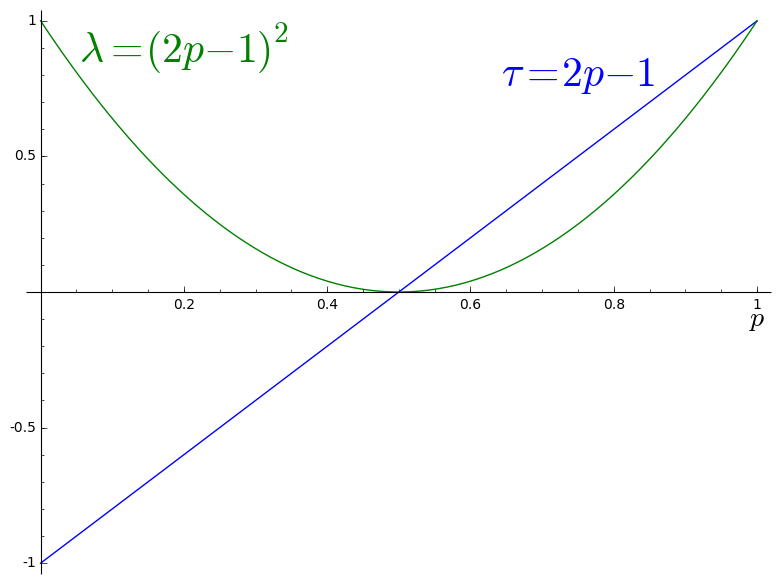
\includegraphics[scale=0.5]{figures/BC_Potenzial2.png}
\end{center}
\caption{Zusammenhang zwischen Wahrscheinlichkeit $p$,
   I/O-Korrela\-tion\index{I/O-Korrelation} $\tau$ und
   Potenzial\index{Potenzial} $\lambda$}\label{fig-bool-pot}
\end{figure}

\begin{sagecode}
\begin{verbatim}

sage: plot1 = plot(2*x-1, (x,0,1))
sage: plot2 = plot((2*x - 1)**2, (x,0,1), color = 'green')
sage: xlabel = text('$p$', (1.0, -0.1), fontsize = 20, color = 'black')
sage: legend1 = text('$\tau = 2p - 1$', (0.75,0.8), fontsize = 30)
sage: legend2 = text('$\lambda = (2p - 1)^2$', (0.2,0.9), fontsize = 30,\\
        color = 'green')
sage: show(plot1 + plot2 + xlabel + legend1 + legend2)
\end{verbatim}
\caption{Plot von I/O-Korrelation\index{I/O-Korrelation} und
   Potenzial\index{Potenzial}}\label{Sage-code-bool-pot}
\end{sagecode}

Der Schl�ssel $k$ ist allerdings das Ziel des Angriffs und die
Wahrscheinlichkeit $p_{F,\alpha,\beta,\kappa}(k)$ in der
Angriffssituation unbekannt. F�r die Kryptoanalyse ist es daher
angebracht, die Wahrscheinlichkeit einer linearen Relation noch
�ber alle Schl�ssel zu mitteln:
\begin{equation}\label{eq-bool-avrg}
   p_{F,\alpha,\beta,\kappa} := \frac{1}{2^{n+l}}
      \#\{(a,k) \in \F_2^n \times \F_2^l \:|\:
           \kappa(k) = \alpha(a) + \beta(F(a,k)) \}.
\end{equation}
Diese Gr��e ist, zumindest theoretisch, wenn man die Effizienzfrage
au�er Acht l�sst, allein aus der Definition der Chiffre $F$ bestimmbar.
Ihre Bestimmung l�uft allerdings auf eine Exhaustion aller Klartexte
und Schl�ssel hinaus und ist daher bei einer realen Chiffre mit
gen�gend gro�en Blockl�ngen oft wirklich nur theoretisch.
Auch hierf�r werden  I/O-Korrelation\index{I/O-Korrelation} und
Potenzial\index{Potenzial} definiert:
\[
   \tau_{F,\alpha,\beta,\kappa} := 2 p_{F,\alpha,\beta,\kappa} - 1,
\]
\[
   \lambda_{F,\alpha,\beta,\kappa} := \tau_{F,\alpha,\beta,\kappa}^2.
\]

Shamir\index{Shamir, Adi}\footnote{%
  Adi Shamir, israelischer Kryptologe, Miterfinder des RSA-Verfahrens,
  $~^{\ast}$6.7.1952.
}
bemerkte schon 1985, dass es �berzuf�llige lineare
Relationen\index{lineare Relation}\index{Relation!linear}
f�r die S-Boxen des DES\index{DES}-Verfahrens gibt. Es dauerte allerdings weitere
sieben Jahre, bis es Matsui\index{Matsui, Mitsuru}\footnote{%
  Mitsuru Matsui, japanischer Kryptologe, $~^{\ast}$16.9.1961.
}
(nach ersten Versuchen von Gilbert und Chass� 1990 mit der Chiffre FEAL)
gelang, diese Beobachtung systematisch
auszunutzen. Er ging zur Sch�tzung\index{Maximum-Likelihood-Sch�tzung}\footnote{%
   Das ist eine sogenannte Maximum-Likelihood-Sch�tzung, d.\,h.,
   man entscheidet sich f�r diejenige von mehreren Hypothesen (hier
   sind es nur zwei), unter deren Annahme das Beobachtungsergebnis
   die h�chste Wahrscheinlichkeit hat.
} von $\kappa(k)$ wie folgt vor
(im Fall $p_{F,\alpha,\beta,\kappa} > \frac{1}{2}$, sonst muss man
bei der Entscheidung die Werte $0$ und $1$ vertauschen\footnote{%
  Im Fall $p_{F,\alpha,\beta,\kappa} = \frac{1}{2}$ ist die
  Methode in dieser Form unbrauchbar.
}):
\begin{enumerate}
	\item {\bf [Sammelphase]} Man sammelt $N$ Klartext-Geheimtextpaare
	  $(a_1,c_1), \ldots, (a_N,c_N)$.

	\item {\bf [Ausz�hlung]} Man bestimmt die Anzahl
\[
    t := \# \{i = 1, \ldots, N \:|\: \alpha(a_i) + \beta(c_i) = 0\}.
\]

	\item {\bf [Mehrheitsentscheidung]} aufgrund von $t$:
	  \begin{itemize}
	    \item Ist $t > \frac{N}{2}$, sch�tzt man $\kappa(k) = 0$.
	    \item Ist $t < \frac{N}{2}$, sch�tzt man $\kappa(k) = 1$.
	  \end{itemize}
\end{enumerate}
Der Fall $t = \frac{N}{2}$ ist unergiebig, kommt aber selten vor -- man
entscheidet zuf�llig zwischen $0$ und $1$ oder gibt eine entsprechende
R�ckmeldung\footnote{%
   am besten beides wie im SageMath-Beispiel~\ref{Sage-code-bool-mats}
}. Im SageMath-Beispiel~\ref{Sage-code-bool-mats}
steht der Programmcode, eine konkrete Anwendung folgt gleich als Beispiel
im n�chsten Unterabschnitt.

\begin{sagecode}
\begin{verbatim}

def Matsui_Test(a, b, pc, compl = False):
  """Matsui's test for linear cryptanalysis"""
  N = len(pc)
  results = []
  for pair in pc:
    ax = binScPr(a,pair[0])
    by = binScPr(b,pair[1])
    result = (ax + by) % 2
    results.append(result)
  t = 0
  for bb in results:
    if bb == 0:
      t = t + 1
  if 2*t > N:
    if compl:
      return [t,1,True]
    else:
      return [t,0,True]
  elif 2*t_0 < N:
    if compl:
      return [t,0,True]
    else:
      return [t,1,True]
  else:
    return [t,randint(0,1),False]
\end{verbatim}
\caption{Matsui-Test\index{Matsui-Test}. Die Linearformen sind {\tt a} f�r $\alpha$ und
   {\tt b} f�r $\beta$. Die Liste {\tt pc} enth�lt {\tt N} Paare von Klartext
   und Geheimtext. Der Boolesche Wert {\tt compl} gibt an, ob das
   als Ergebnis gesch�tzte Bit invertiert werden soll. Die Ausgabe
   ist ein Tripel aus der Anzahl {\tt t} der gez�hlten Nullen,
   dem gesch�tzten Bit und einem Booleschen Wert, der angibt, ob das
   Bit deterministisch bestimmt ({\tt True}) oder im Grenzfall
   zuf�llig bestimmt ({\tt False}) wurde. Verwendet wird die Funktion
   {\tt binScPr} aus dem SageMath-Beispiel~\ref{Sage-code-bool-div-bbl}
   im Anhang~\ref{ss-bool-conv}.}\label{Sage-code-bool-mats}
\end{sagecode}

Wenn man eine lineare Relation\index{lineare Relation}\index{Relation!linear}
mit hinreichend gro�em Potenzial\index{Potenzial}, d.\,h.
hinreichend weit von $\frac{1}{2}$ abweichender Wahrscheinlichkeit, erwischt hat,
wird die Erfolgswahrscheinlichkeit dieses Verfahrens bei hinreichend
gro�em $N$ gut sein. Das erlaubt dann, die Anzahl der unbekannten
Schl�sselbits durch Elimination\index{Elimination} um 1 zu verringern.

Als theoretisches Ergebnis aus diesen �berlegungen
werden wir einen Zusammenhang zwischen der Anzahl $N$ von
ben�tigten Klartextbl�cken und der Erfolgswahrscheinlichkeit erhalten,
siehe Tabelle~\ref{tab-bool-N}.

Je mehr solcher linearen Relationen die Angreiferin mit gen�gend hoher
Gewissheit findet, desto st�rker kann sie die Gr��e des Schl�sselraums
einschr�nken, bis schlie�lich eine Exhaustion\index{Exhaustion} �ber die noch in Frage
kommenden Schl�ssel in den Bereich des Machbaren r�ckt. Ein konkretes
Beispiel in Abschnitt~\ref{ss-bool-mini} wird dies illustrieren.

\subsubsection*{Beispiel}

F�r ein konkretes Beispiel mit $n = l = 4$ betrachten wir die
Boolesche Abbildung\footnote{%
   $f$ ist nebenbei bemerkt die S-Box\index{S-Box} $\mathrm{S}_0$
   von {\sc Lucifer}\index{Lucifer},
   das um 1970 als Vorg�nger-Verfahren von DES\index{DES} entwickelt wurde.
} $f$, die durch die Wertetabelle~\ref{tab-bool-A1}
gegeben ist, und bilden damit die Bitblock-Chiffre
(s.\,a. Abbildung~\ref{fig-bool-bsp0})
\[
    F\!: \F_2^4 \times \F_2^4 \longrightarrow \F_2^4, \quad
    F(a,k) := f(a + k).
\]
Das SageMath-Beispiel~\ref{Sage-code-Luc-S0} definiert diese Boolesche
Abbildung $f$ unter dem Namen {\tt S0}
und verwendet die Klassen {\tt BoolF} und {\tt BoolMap} aus dem
Anhang~\ref{ss-bool-class}. Dabei geben die Spalten der (impliziten)
definierenden Matrix genau die Werte der Abbildung an, wie man sie auch
in Tabelle~\ref{tab-bool-A1} in der Spalte $y = f(x)$ wiederfindet.
(D.\,h., das SageMath-Beispiel~\ref{Sage-code-Luc-S0} und die
Tabelle~\ref{tab-bool-A1} enthalten �quivalente Definitionen der
Abbildung $f$.)
Eine exemplarische Evaluation illustriert das (f�r die dritte Spalte,
entsprechend dem Argument {\tt 0010}).

\begin{sagecode}
\begin{verbatim}

f1 = BoolF([1,1,0,1,1,1,1,0,0,0,0,0,1,0,0,1])
f2 = BoolF([1,1,1,0,1,1,0,0,0,1,0,0,0,1,1,0])
f3 = BoolF([0,1,1,1,1,0,1,0,1,1,1,0,0,0,0,0])
f4 = BoolF([0,1,1,0,0,1,1,0,0,0,1,1,1,0,1,0])
S0 = BoolMap([f1,f2,f3,f4])
# Sample evaluation
sage: S0.valueAt([0,0,1,0])
[0, 1, 1, 1]
\end{verbatim}
\caption{Eine Boolesche Abbildung (S-Box $\mathrm{S}_0$ von
   {\sc Lucifer})}\label{Sage-code-Luc-S0}
\end{sagecode}

Wir verschl�sseln mit dem Schl�ssel $k =$ \verb:1000:, den wir sp�ter zur
Probe angreifen wollen. F�r eine lineare Relation betrachten wir die
Linearformen
\[
     \alpha(a) = a_4, \quad \beta(c) = c_1 + c_2 + c_4, \quad \kappa(k) = k_4;
\]
wir werden in Abschnitt~\ref{ss-bool-bsp1} sehen, dass mit diesen
Linearformen die Relation
$\kappa(k) = \alpha(a) + \beta(c)$ f�r $F$ eine Wahrscheinlichkeit
deutlich $> \frac{1}{2}$ hat. Tabelle~\ref{tab-bool-mats} zeigt die
Verschl�sselung dreier Klartexte $a$, die wir sp�ter als bekannte
Klartexte annehmen wollen. Die Werte f�r $c$ wurden aus der
Wertetabelle~\ref{tab-bool-A1} abgelesen. Die Anzahl $t$ der
beobachteten Werte $0$ von $\alpha(a)$ + $\beta(c)$ ist $t = 2$.
Die Mehrheitsentscheidung f�hrt also zu der Sch�tzung $k_4 = 0$
(von der wir wissen, dass sie korrekt ist).

\begin{table}
\begin{center}
\begin{tabular}{|c|c|c|c|} \hline
       $x$   & $y=f(x)$& $\alpha(x) = x_4$ & $\beta(y) = y_1+y_2+y_4$ \\ \hline
     0 0 0 0 & 1 1 0 0 &   0   &  0  \\
     0 0 0 1 & 1 1 1 1 &   1   &  1  \\
     0 0 1 0 & 0 1 1 1 &   0   &  0  \\
     0 0 1 1 & 1 0 1 0 &   1   &  1  \\
     0 1 0 0 & 1 1 1 0 &   0   &  0  \\
     0 1 0 1 & 1 1 0 1 &   1   &  1  \\
     0 1 1 0 & 1 0 1 1 &   0   &  0  \\
     0 1 1 1 & 0 0 0 0 &   1   &  0  \\
     1 0 0 0 & 0 0 1 0 &   0   &  0  \\
     1 0 0 1 & 0 1 1 0 &   1   &  1  \\
     1 0 1 0 & 0 0 1 1 &   0   &  1  \\
     1 0 1 1 & 0 0 0 1 &   1   &  1  \\
     1 1 0 0 & 1 0 0 1 &   0   &  0  \\
     1 1 0 1 & 0 1 0 0 &   1   &  1  \\
     1 1 1 0 & 0 1 0 1 &   0   &  0  \\
     1 1 1 1 & 1 0 0 0 &   1   &  1  \\ \hline
\end{tabular}
\end{center}
\caption{Wertetabelle einer Booleschen Abbildung
  $f\!: \F_2^4 \longrightarrow \F_2^4$ und zwei Linearformen}\label{tab-bool-A1}
\end{table}

\begin{table}
\begin{center}
\begin{tabular}{|c|c|c||ccc|}\hline
   $a$  & $a+k$ & $c$  & $\alpha(a)$ & $\beta(c)$ & $\alpha(a)$ + $\beta(c)$ \\
   \hline
   0010 & 1010  & 0011 &     0       &      1     &             1            \\
   0101 & 1101  & 0100 &     1       &      1     &             0            \\
   1010 & 0010  & 0111 &     0       &      0     &             0            \\
   \hline
\end{tabular}
\end{center}
\caption{Sch�tzung eines Schl�sselbits nach Matsui unter Verwendung von drei
   bekannten Klartexten}\label{tab-bool-mats}
\end{table}

Das war mit dem Bleistift auf Papier ganz leicht auszuz�hlen. Dennoch
ist der Nachvollzug in SageMath im Hinblick auf kompliziertere Beispiele
instruktiv. Das geschieht im SageMath-Beispiel~\ref{Sage-code-Mats-Expl}.
Dabei wird die Funktion {\tt xor}\index{XOR} aus dem
SageMath-Beispiel~\ref{Sage-code-bool-div-bbl} im Anhang~\ref{ss-bool-conv}
sowie die im SageMath-Beispiel~\ref{Sage-code-Luc-S0}
definierte Abbildung {\tt S0} verwendet. Das Ergebnis \mbox{\tt [2, 0, True]}
besagt, dass $2$ Nullen unter den ausgez�hlten Werten waren, was zur
Mehrheitsentscheidung $0$ f�hrt, die (wegen {\tt True}) nicht durch
zuf�llige Auslosung bei Gleichstand ermittelt wurde.

\begin{sagecode}
\begin{verbatim}

sage: k = [1,0,0,0]
sage: alpha = [0,0,0,1]
sage: beta = [1,1,0,1]
sage: plist = [[0,0,1,0],[0,1,0,1],[1,0,1,0]]
sage: xlist = []
sage: xclist = []
sage: pclist = []
sage: for i in range(0,len(plist)):
....:     x = xor(plist[i],k)
....:     xlist.append(x)
....:
sage: xlist
[[1, 0, 1, 0], [1, 1, 0, 1], [0, 0, 1, 0]]
sage: for i in range(0,len(plist)):
....:     val = S0.valueAt(xlist[i])
....:     xclist.append([xlist[i],val])
....:     pclist.append([plist[i],val])
....:
sage: Matsui_Test(alpha,beta,pclist,False)
[2, 0, True]
\end{verbatim}
\caption{Ein Beispiel f�r den Matsui-Test\index{Matsui-Test}}\label{Sage-code-Mats-Expl}
\end{sagecode}

\noindent Damit das Verfahren im allgemeinen Fall Erfolg verspricht, sind
folgende Fragen zu kl�ren:
\begin{enumerate}
	\item Wie findet man lineare
        Relationen\index{lineare Relation}\index{Relation!linear}
        von m�glichst auff�lliger
        Wahrscheinlichkeit? Insbesondere im Hinblick darauf, dass die
        Auswertung der Formel~(\ref{eq-bool-avrg}) am Effizienzproblem
        scheitert.
     \item Da Bitblock-Chiffren\index{Bitblock-Chiffre} meistens aus
        vielen Runden\index{Runde} zusammengesetzt sind, fragt man weiter:
	\begin{enumerate}
	  \item Wie findet man bei einer iterierten Bitblock-Chiffre
	    brauchbare lineare Relationen f�r die Rundenfunktion?
	  \item Wie setzt man diese �ber die Runden hinweg zu linearen Relationen
	    f�r die ganze Chiffre zusammen?
	  \item Wie bestimmt man die Wahrscheinlichkeit einer zusammengesetzten
	    linearen Relation f�r die ganze Chiffre aus der f�r die einzelnen
	    Runden?
	\end{enumerate}
\end{enumerate}

\noindent Die Antwort auf die erste Frage und Teil (a) der zweiten hei�t:
Aus dem linearen Profil\index{lineares Profil}\index{Profil!linear},
siehe Abschnitt~\ref{ss-bool-lpr}. Die anschlie�enden
Teilfragen f�hren zur Untersuchung von linearen
Pfaden\index{linearer Pfad}\index{Pfad!linear},
siehe Abschnitt~\ref{ss-bool-path}, und zur Kumulation von
Wahrscheinlichkeiten, siehe Satz~\ref{thm-bool-rrnd}. F�r (c) kommt
dabei letztendlich eine brauchbare Faustregel heraus.

\subsection{Beispiel A: Eine Einrunden-Chiffre}\label{ss-bool-bsp1}

Es werden Beispiele betrachtet, die als ernsthafte Blockchiffren viel
zu einfach sind, aber das Prinzip der linearen
Kryptoanalyse\index{lineare Kryptoanalyse}\index{Kryptoanalyse!linear}
anschaulich und nachvollziehbar demonstrieren. Dabei werden stets
Rundenfunktionen der Gestalt $f(a+k)$ betrachtet, d.\,h., der Schl�ssel
bzw. ein $n$-bittiger Teil davon wird vor der Anwendung einer bijektiven
S-Box $f\!: \F_2^n \longrightarrow \F_2^n$ bin�r auf den Klartext
aufaddiert\footnote{%
   Das ist zwar eine sehr spezielle Art, den Schl�ssel in das Verfahren
   einzubringen, aber dennoch realistisch. Die paradigmatischen
   Beispiel-Chiffren {\sc Lucifer}\index{Lucifer}, DES\index{DES}
   und AES\index{AES} verfahren so.
   Bei AES \cite{DaRi2002} hei�t das \glqq key-alternating cipher structure\grqq.
}. Das einfachste denkbare Modell, die Verschl�sselung nach der
Vorschrift
\[
   c = f(a+k)
\]
wie im Beispiel des Abschnitts~\ref{ss-bool-lka},
siehe Abbildung~\ref{fig-bool-bsp0}\footnote{%
  In den grafischen Darstellungen hier und sp�ter wird die Abbildung
  $f$ auf der elementweisen Ebene durch die S-Box S repr�sentiert.
},
ist dabei witzlos, da bei bekanntem\index{bekannter Klartext}\index{Klartext!bekannt}
Klartext die Gleichung nach dem
Schl�ssel $k$ aufl�sbar ist\footnote{%
  Die Umkehrabbildung $f^{-1}$ wird hier als der Angreiferin
  bekannt angenommen. Sie ist ja Teil des Algorithmus zur Entschl�sselung.
  Einweg-Verschl�sselungen\index{Einweg-Verschl�sselung},
  bei denen $f^{-1}$ aus $f$ nicht effizient
  herleitbar ist, bilden ein anderes Kapitel der Kryptographie.
}:
\[
   k = f^{-1}(c) + a.
\]

\begin{figure}
\begin{center}
\begin{picture}(268,68)(0,0)
% Mengen
   \put(11,14){$\F_2^n$}
   \put(28,17){\vector(1,0){34}}
   \put(66,14){$\F_2^n$}
   \put(54,26){$\bigoplus$}
   \put(66,54){$\F_2^n$}
   \put(71,51){\vector(0,-1){28}}
   \put(83,17){\vector(1,0){34}}
   \put(94,20){$f$}
   \put(123,14){$\F_2^n$}

% Elemente
   \put(154,14){$a$}
   \put(165,17){\vector(1,0){28}}
   \put(165,14){\line(0,1){6}}
   \put(197,14){$b$}
   \put(197,54){$k$}
   \put(199,51){\vector(0,-1){28}}
   \put(197,51){\line(1,0){6}}
   \put(205,17){\vector(1,0){40}}
   \put(205,14){\line(0,1){6}}
   \put(214,14){\fcolorbox{black}{yellow}{S}}
   \put(251,14){$c$}

% Rahmen
   \put(0,0){\line(1,0){268}}
   \put(0,68){\line(1,0){268}}
   \put(0,0){\line(0,1){68}}
   \put(268,0){\line(0,1){68}}
\end{picture}
\end{center}
\caption{Ein (viel) zu einfaches Beispiel}\label{fig-bool-bsp0}
\end{figure}

\begin{figure}
\begin{center}
\begin{picture}(208,137)(0,0)
% Mengen
   \put(11,83){$\F_2^n$}
   \put(28,85){\vector(1,0){34}}
   \put(66,83){$\F_2^n$}
   \put(54,94){$\bigoplus$}
   \put(66,124){$\F_2^n$}
   \put(71,120){\vector(0,-1){28}}
   \put(83,85){\vector(1,0){34}}
   \put(94,88){$f$}
   \put(125,83){$\F_2^n$}
   \put(140,85){\vector(1,0){34}}
   \put(179,124){$\F_2^n$}
   \put(185,120){\vector(0,-1){28}}
   \put(168,94){$\bigoplus$}
   \put(179,83){$\F_2^n$}

% Elemente
   \put(23,14){$a$}
   \put(34,17){\vector(1,0){28}}
   \put(34,14){\line(0,1){6}}
   \put(71,14){$b$}
   \put(68,54){$k^{(0)}$}
   \put(74,51){\vector(0,-1){28}}
   \put(71,51){\line(1,0){6}}
   \put(80,17){\vector(1,0){40}}
   \put(80,14){\line(0,1){6}}
   \put(91,14){\fcolorbox{black}{yellow}{S}}
   \put(128,14){$b'$}
   \put(179,54){$k^{(1)}$}
   \put(185,51){\vector(0,-1){28}}
   \put(182,51){\line(1,0){6}}
   \put(142,17){\vector(1,0){28}}
   \put(142,14){\line(0,1){6}}
   \put(182,14){$c$}

% Rahmen
   \put(0,0){\line(1,0){208}}
   \put(0,137){\line(1,0){208}}
   \put(0,0){\line(0,1){137}}
   \put(208,0){\line(0,1){137}}
\end{picture}
\end{center}
\caption{Beispiel A: Eine Einrunden-Chiffre}\label{fig-bool-bspA}
\end{figure}

\begin{figure}
\begin{center}
\begin{picture}(85,68)(0,0)
   \put(6,48){$\F_2^n$}
   \put(23,51){\vector(1,0){40}}
   \put(40,54){$f$}
   \put(68,48){$\F_2^n$}
   \put(40,9){$\F_2$}
   \put(17,43){\vector(1,-1){23}}
   \put(17,26){$\alpha$}
   \put(68,43){\vector(-1,-1){23}}
   \put(60,26){$\beta$}
   \put(38,31){$\stackrel{p}{\approx}$}

% Rahmen
   \put(0,0){\line(1,0){85}}
   \put(0,68){\line(1,0){85}}
   \put(0,0){\line(0,1){68}}
   \put(85,0){\line(0,1){68}}
\end{picture}
\end{center}
\caption{Diagramm f�r eine "`approximative"' lineare
   Relation\index{lineare Relation}\index{Relation!linear}}\label{fig-bool-appr}
\end{figure}

Dieser einfache Angriff wird bei dem etwas komplizierteren Beispiel A mit
\[
   c = f(a+k^{(0)}) + k^{(1)}
\]
verhindert (siehe Abbildung~\ref{fig-bool-bspA}); hier ist der Ansatz der linearen
Kryptoanalyse\index{lineare Kryptoanalyse}\index{Kryptoanalyse!linear}
bereits sinnvoll: Sei $(\alpha,\beta)$ ein Paar von Linearformen\index{Linearform}
mit
\begin{equation}\label{eq-bool-prob}
     \beta\circ f(x) \stackrel{p}{\approx} \alpha(x),
\end{equation}
wobei das Symbol $\stackrel{p}{\approx}$ zu lesen ist als
"`gleich mit Wahrscheinlichkeit $p$"', also
\[
     p = p_{f,\alpha,\beta} :=
     \frac{1}{2^{n}} \cdot \#\{x \in \F_2^n \:|\: \beta\circ f(x) = \alpha(x) \}.
\]
Repr�sentiert wird die Formel~(\ref{eq-bool-prob}) durch das Diagramm in
Abbildung~\ref{fig-bool-appr}. Die Linearform $\kappa$ der
allgemeinen Theorie tritt hier nicht explizit auf: Da die
Schl�sselbits auf Klartext und ("`intermedi�ren"') Geheimtext einfach
aufaddiert werden, ist $\kappa = \alpha$ f�r $k^{(0)}$ und $\kappa = \beta$
f�r $k^{(1)}$, also $\kappa(k^{(0)}, k^{(1)}) = \alpha(k^{(0)}) + \beta(k^{(1)})$.

Wie h�ngt das mit der allgemeinen Situation aus Abschnitt~\ref{ss-bool-lka}
zusammen? F�r das Beispiel~A ist
\begin{itemize}
   \item die Schl�ssell�nge $l = 2n$, der Schl�sselraum ist $\F_2^{2n}$, und
      Schl�ssel haben die Gestalt $k = (k^{(0)},k^{(1)})$ mit $k^{(0)}, k^{(1)} \in \F_2^n$.
   \item Die Chiffre ist durch die Abbildung
\[
     F\!: \F_2^n \times \F_2^n \times \F_2^n \longrightarrow \F_2^n,
     \quad (a, k^{(0)}, k^{(1)}) \mapsto f(a + k^{(0)}) + k^{(1)},
\]
      definiert.
   \item Die Linearform $\kappa\!: \F_2^n \times \F_2^n \longrightarrow \F_2$
      ist durch $\kappa(k^{(0)},k^{(1)}) = \alpha(k^{(0)}) + \beta(k^{(1)})$ gegeben.
\end{itemize}
Die Wahrscheinlichkeit einer linearen Relation f�r einen festen
Schl�ssel \mbox{$k = (k^{(0)},k^{(1)})$} ist damit
\begin{eqnarray*}
    p_{F,\alpha,\beta,\kappa}(k) & = & \frac{1}{2^n} \cdot
      \#\{a \in \F_2^n \:|\: \kappa(k) = \alpha(a) + \beta(F(a,k)) \} \\
     & = & \frac{1}{2^n} \cdot
      \#\{a \in \F_2^n \:|\: \alpha(k^{(0)}) + \beta(k^{(1)}) = \alpha(a) + \beta(f(a + k^{(0)}) + k^{(1)}) \} \\
     & = & \frac{1}{2^n} \cdot
      \#\{a \in \F_2^n \:|\: \alpha(k^{(0)}) = \alpha(a) + \beta(f(a + k^{(0)})) \},
\end{eqnarray*}
da $\beta(k^{(1)})$ auf beiden Seiten der Gleichung innerhalb der Mengenklammern
vorkommt und daher einfach weggelassen werden kann.

Dieser Ausdruck ist unabh�ngig von $k^{(1)}$, und an der leicht umgeformten
Gleichung
\[
     p_{F,\alpha,\beta,\kappa}(k) = \frac{1}{2^n} \cdot
      \#\{a \in \F_2^n \:|\: \alpha(a + k^{(0)}) = \beta(f(a + k^{(0)})) \}
\]
sieht man, dass er f�r alle $k^{(0)}$ den gleichen Wert hat, da bei festem
$k^{(0)}$ mit $a$ auch $a + k^{(0)}$ ganz $\F_2^n$ durchl�uft. Dieser Wert
muss daher mit dem Mittelwert �ber alle $k$ �bereinstimmen:
\[
     p_{F,\alpha,\beta,\kappa}(k) = p_{F,\alpha,\beta,\kappa} = \frac{1}{2^n} \cdot
      \#\{x \in \F_2^n \:|\: \alpha(x) = \beta(f(x)) \} = p.
\]
Mit dieser �berlegung ist gezeigt:

\begin{satz}
    In der Situation des Beispiels~A nimmt die Wahrscheinlichkeit $p_{F,\alpha,\beta,\kappa}(k)$
    f�r jeden Schl�ssel $k \in \F_2^{2n}$ den gleichen Wert
\[
     p = \frac{1}{2^n} \cdot \#\{x \in \F_2^n \:|\: \alpha(x) = \beta(f(x)) \}
\]
   an, insbesondere ist $p$ auch der Mittelwert nach Gleichung~(\ref{eq-bool-avrg}).
\end{satz}

Mit den Bezeichnungen aus Abbildung~\ref{fig-bool-bspA} gilt nun
\begin{align*}
   \beta(c) & = \beta(b' + k^{(1)}) = \beta(b') + \beta(k^{(1)}) \\
            & \stackrel{p}{\approx} \alpha(b) + \beta(k^{(1)})
                   = \alpha(a + k^{(0)}) + \beta(k^{(1)})
                        = \alpha(a) + \alpha(k^{(0)}) + \beta(k^{(1)}).
\end{align*}
Als lineare Relation\index{lineare Relation}\index{Relation!linear}
f�r die Bits des Schl�ssels $k = (k^{(0)},k^{(1)})$ erhalten wir
\[
   \alpha(k^{(0)}) + \beta(k^{(1)}) \stackrel{p}{\approx} \alpha(a) + \beta(c).
\]
Ein analoger Schluss l�sst sich f�r die komplement�re Relation
\[
   \beta\circ f(x) \stackrel{1-p}{\approx} \alpha(x) + 1
\]
durchf�hren. Insgesamt ist damit gezeigt:

\begin{satz}
  Im Beispiel~A sei $(\alpha,\beta)$ ein Paar von Linearformen\index{Linearform} f�r $f$
  mit der Wahrscheinlichkeit $p$ wie in Formel~(\ref{eq-bool-prob}).
  Dann ist $\hat{p} =$ \mbox{$\max\{p, 1-p\}$} die Erfolgswahrscheinlichkeit f�r
  die Bestimmung eines Schl�sselbits aus {\em einem} bekannten
  Klartext\index{bekannter Klartext}\index{Klartext!bekannt}
  durch diese lineare Relation\index{lineare Relation}\index{Relation!linear}.
\end{satz}

\subsubsection*{Beispiel}

Nehmen wir als konkretes Beispiel $n = 4$ und f�r $f$ wieder die S-Box
$\mathrm{S}_0$ von {\sc Lucifer}\index{Lucifer}. Die beiden rechten Spalten der
Tabelle~\ref{tab-bool-A1} zeigen, dass die durch $(\alpha,\beta)$ mit $\alpha(x) = x_4$
und $\beta(y) = y_1+y_2+y_4$ definierte lineare Relation die Wahrscheinlichkeit
$p_{f,\alpha,\beta} = \frac{14}{16} = \frac{7}{8}$ hat\footnote{%
  Deren Gr��e ist ein starkes Indiz daf�r, dass die Designer von
  {\sc Lucifer}\index{Lucifer} die lineare
  Kryptoanalyse\index{lineare Kryptoanalyse}\index{Kryptoanalyse!linear}
  noch nicht kannten.
}.

Die konkreten Rundenschl�ssel\index{Rundenschl�ssel} seien
$k^{(0)} =$ \verb:1000: und $k^{(1)} =$ \verb:0001:.
Die Tabelle~\ref{tab-bool-linrel} �ber alle $16$ m�glichen
Klartexte zeigt, dass $\alpha(a)+\beta(c)$ den Wert $1 =\alpha(k^{(0)}) + \beta(k^{(1)})$
f�r die Summe der Schl�sselbits genau $14$-mal annimmt, wie es sein soll.

\begin{table}
\begin{center}
\begin{tabular}{|cccc|c|} \hline
  $a$  & $b$  & $b'$ & $c$  & $\alpha(a)+\beta(c) = a_4 + c_1 + c_2 + c_4$ \\ \hline
  0000 & 1000 & 0010 & 0011 & 1 \\
  0001 & 1001 & 0110 & 0111 & 1 \\
  0010 & 1010 & 0011 & 0010 & 0 \\
  0011 & 1011 & 0001 & 0000 & 1 \\
  0100 & 1100 & 1001 & 1000 & 1 \\
  0101 & 1101 & 0100 & 0101 & 1 \\
  0110 & 1110 & 0101 & 0100 & 1 \\
  0111 & 1111 & 1000 & 1001 & 1 \\
  1000 & 0000 & 1100 & 1101 & 1 \\
  1001 & 0001 & 1111 & 1110 & 1 \\
  1010 & 0010 & 0111 & 0110 & 1 \\
  1011 & 0011 & 1010 & 1011 & 1 \\
  1100 & 0100 & 1110 & 1111 & 1 \\
  1101 & 0101 & 1101 & 1100 & 1 \\
  1110 & 0110 & 1011 & 1010 & 1 \\
  1111 & 0111 & 0000 & 0001 & 0 \\
  \hline
\end{tabular}
\end{center}
\caption{Eine lineare Relation f�r die Schl�sselbits ($b$ entsteht aus $a$ durch Addition
   von $k^{(0)}$, also ``Umkippen'' des ersten Bits, $b'$ aus $b$ durch Anwendung
   von $f$, $c$ aus $b'$ durch Addition von $k^{(1)}$.}\label{tab-bool-linrel}
\end{table}

Wie gro� ist nun die Erfolgswahrscheinlichkeit $p_N$ daf�r, diesen Wert
richtig zu sch�tzen, wenn man $N = 1, 2, \ldots$ zuf�llige bekannte
Klartexte\index{bekannter Klartext}\index{Klartext!bekannt}
aus der Menge der $2^n$ m�glichen zur Verf�gung hat (zu gegebenen festen
Linearformen $\alpha$ und $\beta$ mit $p = p_{f,\alpha,\beta}$)? Das ist genau
eine konkrete Einkleidung der Fragestellung der hypergeometrischen Verteilung,
und daher gilt
(ohne Beweis und ohne Erkl�rung der hypergeometrischen
Verteilung\index{hypergeometrische Verteilung}\index{Verteilung!hypergeometrisch}):

\begin{satz}
  Im Beispiel A sei $(\alpha,\beta)$ ein Paar von Linearformen, das
  eine lineare Relation f�r $f$ mit der Wahrscheinlichkeit $p$ definiert.
  Dann ist die Erfolgswahrscheinlichkeit f�r die Bestimmung eines
  Schl�sselbits aus $N$ bekannten Klartexten durch diese lineare
  Relation\index{lineare Relation}\index{Relation!linear}
  gerade die kumulierte Wahrscheinlichkeit $p_N = p_N^{(s)}$ der
  hypergeometrischen Verteilung zu den Parametern $2^n$, $s = \hat{p}\cdot 2^n$
  und $N$ mit $\hat{p} = \max\{p, 1-p\}$.
\end{satz}

Verl�sst man die exakte Mathematik und geht, wie oft in der angewandten Statistik,
zu asymptotischen N�herungsformeln �ber, so kann man unter den (sehr vage
formulierten) Voraussetzungen
"`$p$ nicht zu weit von $\frac{1}{2}$ entfernt, $N \ll 2^n$, aber $N$ nicht
zu klein,"' die hypergeometrische Verteilung\index{hypergeometrische
Verteilung}\index{Verteilung!hypergeometrisch} durch die
Normalverteilung\index{Normalverteilung} approximieren und erh�lt
\begin{equation}\label{equ-bool-N}
  p_N \approx \frac{1}{\sqrt{2\pi}} \cdot
                      \int_{-\infty}^{\sqrt{N\lambda}} e^{-t^2/2}\,dt,
\end{equation}
wobei $\lambda = (2p - 1)^2$ das Potenzial\index{Potenzial} der linearen Relation ist.
Zusammen mit den bekannten Werten f�r die Normalverteilung\footnote{%
   Man kann statt mit der Approximation durch die Normalverteilung auch direkt
   mit der hypergeometrischen
   Verteilung\index{hypergeometrische Verteilung}\index{Verteilung!hypergeometrisch}
   rechnen. Dann erh�lt man,
   besonders bei kleinem $N$, einen genaueren Wert, aber keine so
   einfache geschlossene Formel wie (\ref{equ-bool-N}).
} ergibt das die
Tabelle~\ref{tab-bool-N}. D.\,h., um eine Erfolgswahrscheinlichkeit von etwa
$95\%$ zu erreichen, braucht man $N \approx \frac{3}{\lambda}$ bekannte
Klartexte\index{bekannter Klartext}\index{Klartext!bekannt}.
Im obigen konkreten Beispiel war $p = \frac{7}{8}$, also $\lambda = \frac{9}{16}$,
und die Zahl der n�tigen bekannten Klartexte f�r die $95$-prozentige
Erfolgswahrscheinlichkeit ist nach der Formel $N \approx 5$. Wir waren,
siehe Tabelle~\ref{tab-bool-mats}, schon mit $N = 3$ erfolgreich gewesen;
das ist nicht sehr �berraschend, denn wie wir jetzt sehen, war
die Erfolgswahrscheinlichkeit daf�r immerhin knapp 90\% (hier ist n�mlich
$N\lambda = \frac{27}{16} \approx 1,68\ldots$)\footnote{%
   Hier wird man die Voraussetzung "`$N$ nicht zu klein"' der Approximation
   durch die Normalverteilung\index{Normalverteilung} zu Recht anzweifeln m�ssen.
   In der Tat kann man leicht die exakten Werte f�r die hypergeometrische
   Verteilung\index{hypergeometrische Verteilung}\index{Verteilung!hypergeometrisch}
   bestimmen:
   Zieht man aus einer Urne mit $16$ Kugeln, von denen $14$ schwarz und
   $2$ wei� sind, zuf�llig $3$ Kugeln, so werden diese mit Wahrscheinlichkeit
   $\frac{26}{40}$ alle drei schwarz sein, und mit Wahrscheinlichkeit
   $\frac{13}{40}$ zwei davon schwarz und eine wei�, also mit Wahrscheinlichkeit
   $\frac{39}{40} = 97,5\%$ mindestens zwei schwarz. Das ist also deutlich
   mehr als die aus der Approximationsformel~(\ref{equ-bool-N}) bestimmten 90\%.
   Die �brigen Wahrscheinlichkeiten sind $\frac{1}{40}$ f�r genau eine schwarze
   Kugel und $0$ f�r drei wei�e.
}.

\begin{table}
\begin{center}
  \begin{tabular}{|c|ccccccc|} \hline
		$N\lambda$ & $1$ & $2$ & $3$ & $4$ & \ldots & $8$ & $9$ \\
		$p_N$ & $84,1\%$ & $92,1\%$ & $95,8\%$ & $97,7\%$ & \ldots &
		                      $99,8\%$ & $99,9\%$ \\ \hline
  \end{tabular}
\end{center}
\caption{Zusammenhang zwischen der Anzahl der bekannten
   Klartexte\index{bekannter Klartext}\index{Klartext!bekannt}
   und der Erfolgs\-wahr\-schein\-lich\-keit}\label{tab-bool-N}
\end{table}

\subsection{Approximationstabelle\index{Approximationstabelle},
   Korrelationsmatrix\index{Korrelationsmatrix} und lineares
   Profil\index{lineares Profil}\index{Profil!linear}}\label{ss-bool-lpr}

Die H�ufigkeiten, mit denen lineare
Relationen\index{lineare Relation}\index{Relation!linear} f�r eine Boolesche
Abbildung\index{Boolesche Abbildung}\index{Abbildung!Boolesche}
(oder S-Box\index{S-Box}) $f\!: \F_2^n \longrightarrow \F_2^q$ gelten, werden
in einer $2^n \times 2^q$-Matrix zusammengefasst, die zu
jedem Paar von Linearformen\index{Linearform} $(\alpha,\beta)$
die Anzahl der Argumente $x$ mit $\beta\circ f(x) = \alpha(x)$ angibt und
{\bf Approximationstabelle\index{Approximationstabelle}}
genannt wird\footnote{%
   Vorsicht mit den Literatur-Referenzen: Oft wird von allen Eintr�gen
   noch der Wert $2^{n-1}$ abgezogen, so z.\,B. bei der SageMath-Funktion
   {\tt linear\_approximation\_matrix()}.
}\label{fn-lin-appr}.
F�r die oben verwendete S-Box $\mathrm{S}_0$ von {\sc Lucifer}\index{Lucifer}
ist sie in Tabelle~\ref{tab-bool-s0} wiedergegeben. Der Eintrag $16$ in
der linken oberen Ecke besagt, dass die Relation $0 = 0$ immer, also
in allen $16$ F�llen gilt, und ist gleichzeitig der Hauptnenner, durch
den man alle Eintr�ge teilen muss, um die Wahrscheinlichkeiten zu
erhalten; im allgemeinen Fall w�rde dort $2^n$ stehen. Die �brigen Eintr�ge
in der ersten Spalte (entsprechend $\beta = 0$) sind $8$, weil jede von Null
verschiedene Linearform\index{Linearform} $\alpha$ den Wert $0$ in genau der
H�lfte aller F�lle, hier also $8$-mal, annimmt\footnote{%
   In der Sprache der Linearen Algebra\index{lineare Algebra}\index{Algebra!lineare}:
   Der Kern einer Linearform\index{Linearform} $\neq 0$
   ist ein $(n-1)$-dimensionaler Unterraum.
}. F�r die erste Zeile gilt das analoge
Argument -- vorausgesetzt, $f$ ist bijektiv\footnote{%
   Im allgemeinen Fall, wo $q \neq n$ sein kann, m�sste man hier
   "`balanciert\index{balanciert}"' sagen, d.\,h., alle Urbildmengen sind gleich gro�.
   Das geht nat�rlich nur im Fall $q \leq n$ wirklich.
}.

\begin{table}
\begin{center}
\begin{tabular}{|c|cccccccccccccccc|} \hline
     & 0 & 1 & 2 & 3 & 4 & 5 & 6 & 7 & 8 & 9 &10 &11 &12 &13 &14 &15 \\ \hline
   0 &16 & 8 & 8 & 8 & 8 & 8 & 8 & 8 & 8 & 8 & 8 & 8 & 8 & 8 & 8 & 8 \\
   1 & 8 & 6 & 6 & 8 & 8 & 6 & 6 & 8 & 8 & 6 & 6 & 8 & 8 &14 & 6 & 8 \\
   2 & 8 &10 & 8 & 6 & 4 & 6 & 8 & 6 & 6 &12 & 6 & 8 &10 & 8 & 6 & 8 \\
   3 & 8 &12 &10 & 6 &12 & 8 &10 & 6 & 6 & 6 & 8 & 8 &10 &10 & 8 & 8 \\
   4 & 8 & 8 & 4 & 8 & 8 & 8 & 8 & 4 &10 & 6 & 6 & 6 &10 & 6 &10 &10 \\
   5 & 8 &10 &10 &12 & 8 &10 & 6 & 8 &10 & 8 & 4 &10 &10 & 8 & 8 & 6 \\
   6 & 8 &10 & 8 &10 & 8 &10 & 8 &10 & 8 &10 & 8 & 2 & 8 &10 & 8 &10 \\
   7 & 8 & 8 &10 & 6 & 8 & 8 & 2 & 6 & 8 & 8 &10 & 6 & 8 & 8 &10 & 6 \\
   8 & 8 & 8 & 6 &10 & 6 &10 & 8 & 8 & 4 & 8 &10 &10 &10 &10 &12 & 8 \\
   9 & 8 &10 & 8 &10 & 6 & 4 &10 & 8 & 8 & 6 & 8 & 6 & 6 & 8 &10 & 4 \\
  10 & 8 & 6 &10 & 8 & 6 & 8 & 8 &10 & 6 & 4 & 8 & 6 &12 & 6 & 6 & 8 \\
  11 & 8 &12 & 8 & 8 & 6 & 6 & 6 &10 &10 & 6 &10 &10 & 8 & 8 & 8 &12 \\
  12 & 8 & 8 &10 &10 & 6 &10 & 8 & 4 & 6 & 6 & 8 & 8 & 4 & 8 & 6 &10 \\
  13 & 8 & 6 &12 & 6 & 6 & 8 &10 & 8 &10 & 8 & 6 & 8 & 8 &10 &12 & 8 \\
  14 & 8 & 6 &10 &12 &10 & 4 & 8 & 6 & 8 &10 &10 & 8 &10 & 8 & 8 &10 \\
  15 & 8 & 8 & 8 & 8 &10 & 6 & 6 &10 & 4 & 8 & 4 & 8 & 6 & 6 &10 &10 \\ \hline
\end{tabular}
\end{center}
\caption{Approximationstabelle der S-Box $\mathrm{S}_0$ von {\sc Lucifer}\index{Lucifer} --
   Zeilen- und Spaltenindizes sind durch Zahlen repr�sentierte Linearformen,
   siehe Abschnitt~\ref{ss-bool-repr}.
   Die Wahrscheinlichkeiten erh�lt man nach Division durch 16.}\label{tab-bool-s0}
\end{table}

\begin{table}
\begin{center}
\begin{tabular}{|c|cccccccccccccccc|} \hline
     & 0 & 1 & 2 & 3 & 4 & 5 & 6 & 7 & 8 & 9 &10 &11 &12 &13 &14 &15 \\ \hline
   0 & 1 & 0 & 0 & 0 & 0 & 0 & 0 & 0 & 0 & 0 & 0 & 0 & 0 & 0 & 0 & 0 \\
   1 & 0 &$-\frac{1}{4}$&$-\frac{1}{4}$& 0 & 0 &$-\frac{1}{4}$&$-\frac{1}{4}$& 0 & 0 &$-\frac{1}{4}$&$-\frac{1}{4}$& 0 & 0 &$\frac{3}{4}$&$-\frac{1}{4}$& 0 \\
   2 & 0 &$\frac{1}{4}$& 0 & $-\frac{1}{4}$ &$-\frac{1}{2}$& $-\frac{1}{4}$ & 0 & $-\frac{1}{4}$ & $-\frac{1}{4}$ &$\frac{1}{2}$& $-\frac{1}{4}$ & 0 &$\frac{1}{4}$& 0 & $-\frac{1}{4}$ & 0 \\
   3 & 0 &$\frac{1}{2}$&$\frac{1}{4}$& $-\frac{1}{4}$ &$\frac{1}{2}$& 0 &$\frac{1}{4}$& $-\frac{1}{4}$ & $-\frac{1}{4}$ & $-\frac{1}{4}$ & 0 & 0 &$\frac{1}{4}$&$\frac{1}{4}$& 0 & 0 \\
   4 & 0 & 0 &$-\frac{1}{2}$& 0 & 0 & 0 & 0 &$-\frac{1}{2}$&$\frac{1}{4}$& $-\frac{1}{4}$ & $-\frac{1}{4}$ & $-\frac{1}{4}$ &$\frac{1}{4}$& $-\frac{1}{4}$ &$\frac{1}{4}$&$\frac{1}{4}$\\
   5 & 0 &$\frac{1}{4}$&$\frac{1}{4}$&$\frac{1}{2}$& 0 &$\frac{1}{4}$& $-\frac{1}{4}$ & 0 &$\frac{1}{4}$& 0 &$-\frac{1}{2}$&$\frac{1}{4}$&$\frac{1}{4}$& 0 & 0 & $-\frac{1}{4}$ \\
   6 & 0 &$\frac{1}{4}$& 0 &$\frac{1}{4}$& 0 &$\frac{1}{4}$& 0 &$\frac{1}{4}$& 0 &$\frac{1}{4}$& 0 & $-\frac{3}{4}$ & 0 &$\frac{1}{4}$& 0 &$\frac{1}{4}$\\
   7 & 0 & 0 &$\frac{1}{4}$& $-\frac{1}{4}$ & 0 & 0 & $-\frac{3}{4}$ & $-\frac{1}{4}$ & 0 & 0 &$\frac{1}{4}$& $-\frac{1}{4}$ & 0 & 0 &$\frac{1}{4}$& $-\frac{1}{4}$ \\
   8 & 0 & 0 & $-\frac{1}{4}$ &$\frac{1}{4}$& $-\frac{1}{4}$ &$\frac{1}{4}$& 0 & 0 &$-\frac{1}{2}$& 0 &$\frac{1}{4}$&$\frac{1}{4}$&$\frac{1}{4}$&$\frac{1}{4}$&$\frac{1}{2}$& 0 \\
   9 & 0 &$\frac{1}{4}$& 0 &$\frac{1}{4}$& $-\frac{1}{4}$ &$-\frac{1}{2}$&$\frac{1}{4}$& 0 & 0 & $-\frac{1}{4}$ & 0 & $-\frac{1}{4}$ & $-\frac{1}{4}$ & 0 &$\frac{1}{4}$&$-\frac{1}{2}$\\
  10 & 0 & $-\frac{1}{4}$ &$\frac{1}{4}$& 0 & $-\frac{1}{4}$ & 0 & 0 &$\frac{1}{4}$& $-\frac{1}{4}$ &$-\frac{1}{2}$& 0 & $-\frac{1}{4}$ &$\frac{1}{2}$& $-\frac{1}{4}$ & $-\frac{1}{4}$ & 0 \\
  11 & 0 &$\frac{1}{2}$& 0 & 0 & $-\frac{1}{4}$ & $-\frac{1}{4}$ & $-\frac{1}{4}$ &$\frac{1}{4}$&$\frac{1}{4}$& $-\frac{1}{4}$ &$\frac{1}{4}$&$\frac{1}{4}$& 0 & 0 & 0 &$\frac{1}{2}$\\
  12 & 0 & 0 &$\frac{1}{4}$&$\frac{1}{4}$& $-\frac{1}{4}$ &$\frac{1}{4}$& 0 &$-\frac{1}{2}$& $-\frac{1}{4}$ & $-\frac{1}{4}$ & 0 & 0 &$-\frac{1}{2}$& 0 & $-\frac{1}{4}$ &$\frac{1}{4}$\\
  13 & 0 & $-\frac{1}{4}$ &$\frac{1}{2}$& $-\frac{1}{4}$ & $-\frac{1}{4}$ & 0 &$\frac{1}{4}$& 0 &$\frac{1}{4}$& 0 & $-\frac{1}{4}$ & 0 & 0 &$\frac{1}{4}$&$\frac{1}{2}$& 0 \\
  14 & 0 & $-\frac{1}{4}$ &$\frac{1}{4}$&$\frac{1}{2}$&$\frac{1}{4}$&$-\frac{1}{2}$& 0 & $-\frac{1}{4}$ & 0 &$\frac{1}{4}$&$\frac{1}{4}$& 0 &$\frac{1}{4}$& 0 & 0 &$\frac{1}{4}$\\
  15 & 0 & 0 & 0 & 0 &$\frac{1}{4}$& $-\frac{1}{4}$ & $-\frac{1}{4}$ &$\frac{1}{4}$&$-\frac{1}{2}$& 0 &$-\frac{1}{2}$& 0 & $-\frac{1}{4}$ & $-\frac{1}{4}$ &$\frac{1}{4}$&$\frac{1}{4}$\\ \hline
\end{tabular}
\end{center}\caption{Korrelationsmatrix der S-Box $\mathrm{S}_0$ von {\sc Lucifer}\index{Lucifer} --
   Zeilen- und Spaltenindizes sind durch Zahlen repr�sentierte Linearformen.}\label{tab-bool-corr}
\end{table}

\begin{table}
\begin{center}
\begin{tabular}{|c|cccccccccccccccc|} \hline
  &0& 1            & 2            & 3            & 4            & 5            & 6            & 7
     & 8            & 9            &10            &11            &12            &13            &14            &15            \\
\hline
 0&1& 0            & 0            & 0            & 0            & 0            & 0            & 0
     & 0            & 0            & 0            & 0            & 0            & 0            & 0            & 0            \\
 1&0&$\frac{1}{16}$&$\frac{1}{16}$& 0            & 0            &$\frac{1}{16}$&$\frac{1}{16}$& 0
     & 0            &$\frac{1}{16}$&$\frac{1}{16}$& 0            & 0            &$\frac{9}{16}$&$\frac{1}{16}$& 0            \\
 2&0&$\frac{1}{16}$& 0            &$\frac{1}{16}$&$\frac{1}{4}$ &$\frac{1}{16}$& 0            &$\frac{1}{16}$&$\frac{1}{16}$
     &$\frac{1}{4}$ &$\frac{1}{16}$& 0            &$\frac{1}{16}$& 0            &$\frac{1}{16}$& 0            \\
 3&0&$\frac{1}{4}$ &$\frac{1}{16}$&$\frac{1}{16}$&$\frac{1}{4}$ & 0            &$\frac{1}{16}$&$\frac{1}{16}$&$\frac{1}{16}$
     &$\frac{1}{16}$& 0            & 0            &$\frac{1}{16}$&$\frac{1}{16}$& 0            & 0            \\
 4&0& 0            &$\frac{1}{4}$ & 0            & 0            & 0            & 0            &$\frac{1}{4}$ &$\frac{1}{16}$
     &$\frac{1}{16}$&$\frac{1}{16}$&$\frac{1}{16}$&$\frac{1}{16}$&$\frac{1}{16}$&$\frac{1}{16}$&$\frac{1}{16}$\\
 5&0&$\frac{1}{16}$&$\frac{1}{16}$&$\frac{1}{4}$ & 0            &$\frac{1}{16}$&$\frac{1}{16}$& 0            &$\frac{1}{16}$
     & 0            &$\frac{1}{4}$ &$\frac{1}{16}$&$\frac{1}{16}$& 0            & 0            &$\frac{1}{16}$\\
 6&0&$\frac{1}{16}$& 0            &$\frac{1}{16}$& 0            &$\frac{1}{16}$& 0            &$\frac{1}{16}$& 0
     &$\frac{1}{16}$& 0            &$\frac{9}{16}$& 0            &$\frac{1}{16}$& 0            &$\frac{1}{16}$\\
 7&0& 0            &$\frac{1}{16}$&$\frac{1}{16}$& 0            & 0            &$\frac{9}{16}$&$\frac{1}{16}$& 0
     & 0            &$\frac{1}{16}$&$\frac{1}{16}$& 0            & 0            &$\frac{1}{16}$&$\frac{1}{16}$\\
 8&0& 0            &$\frac{1}{16}$&$\frac{1}{16}$&$\frac{1}{16}$&$\frac{1}{16}$& 0            & 0            &$\frac{1}{4}$
     & 0            &$\frac{1}{16}$&$\frac{1}{16}$&$\frac{1}{16}$&$\frac{1}{16}$&$\frac{1}{4}$ & 0            \\
 9&0&$\frac{1}{16}$& 0            &$\frac{1}{16}$&$\frac{1}{16}$&$\frac{1}{4}$&$\frac{1}{16}$& 0            & 0
     &$\frac{1}{16}$& 0            &$\frac{1}{16}$&$\frac{1}{16}$& 0            &$\frac{1}{16}$&$\frac{1}{4}$ \\
10&0&$\frac{1}{16}$&$\frac{1}{16}$& 0            &$\frac{1}{16}$& 0            & 0            &$\frac{1}{16}$&$\frac{1}{16}$
     &$\frac{1}{4}$ & 0            &$\frac{1}{16}$&$\frac{1}{4}$ &$\frac{1}{16}$&$\frac{1}{16}$& 0            \\
11&0&$\frac{1}{4}$ & 0            & 0            &$\frac{1}{16}$&$\frac{1}{16}$&$\frac{1}{16}$&$\frac{1}{16}$&$\frac{1}{16}$
     &$\frac{1}{16}$&$\frac{1}{16}$&$\frac{1}{16}$& 0            & 0            & 0            &$\frac{1}{4}$ \\
12&0& 0            &$\frac{1}{16}$&$\frac{1}{16}$&$\frac{1}{16}$&$\frac{1}{16}$& 0            &$\frac{1}{4}$ &$\frac{1}{16}$
     &$\frac{1}{16}$& 0            & 0            &$\frac{1}{4}$ & 0            &$\frac{1}{16}$&$\frac{1}{16}$\\
13&0&$\frac{1}{16}$&$\frac{1}{4}$&$\frac{1}{16}$&$\frac{1}{16}$& 0            &$\frac{1}{16}$& 0            &$\frac{1}{16}$
     & 0            &$\frac{1}{16}$& 0            & 0            &$\frac{1}{16}$&$\frac{1}{4}$ &$0$\\
14&0&$\frac{1}{16}$&$\frac{1}{16}$&$\frac{1}{4}$ &$\frac{1}{16}$&$\frac{1}{4}$ & 0            &$\frac{1}{16}$& 0
     &$\frac{1}{16}$&$\frac{1}{16}$& 0            &$\frac{1}{16}$& 0            & 0            &$\frac{1}{16}$\\
15&0& 0            & 0            & 0            &$\frac{1}{16}$&$\frac{1}{16}$&$\frac{1}{16}$&$\frac{1}{16}$&$\frac{1}{4}$
     & 0            &$\frac{1}{4}$ & 0            &$\frac{1}{16}$&$\frac{1}{16}$&$\frac{1}{16}$&$\frac{1}{16}$\\
\hline
\end{tabular}
\end{center}\caption{Lineares Profil der S-Box $\mathrm{S}_0$ von {\sc Lucifer}\index{Lucifer} --
   Zeilen- und Spaltenindizes sind durch Zahlen repr�sentierte Linearformen.}\label{tab-bool-lp0}
\end{table}

Die {\bf Korrelationsmatrix}\index{Korrelationsmatrix} und das
{\bf lineare Profil}\index{lineares Profil}\index{Profil!linear}\footnote{%
   oder auch Linearit�tsprofil\index{Linearit�tsprofil}; nicht zu verwechseln
   mit dem linearen
   Komplexit�tsprofil\index{lineares Komplexit�tsprofil}\index{Komplexit�tsprofil!linear} einer
   Bitfolge, das mit Hilfe von linearen Schieberegistern
   definiert wird und auch oft Linearit�tsprofil genannt wird.
   }
sind die entsprechenden Matrizen, deren Eintr�ge
jeweils die I/O-Korrelation\index{I/O-Korrelation} bzw. das
Potenzial\index{Potenzial} der linearen Relation enthalten.
Man erh�lt die Korrelationsmatrix\index{Korrelationsmatrix} aus der
Approximationstabelle\index{Approximationstabelle}, indem man erst
die Eintr�ge durch $2^n$ dividiert, um die jeweiligen Wahrscheinlichkeiten $p$
zu erhalten; dann muss man noch die Wahrscheinlichkeiten nach der Formel
$\tau = 2p - 1$ in I/O-Korrelationen\index{I/O-Korrelation} umrechnen.
Das lineare Profil\index{lineares Profil}\index{Profil!linear}
entsteht dann, indem man die Eintr�ge der
Korrelationsmatrix\index{Korrelationsmatrix} einzeln quadriert.

F�r $\mathrm{S}_0$ ist die Korrelationsmatrix\index{Korrelationsmatrix}
in Tabelle~\ref{tab-bool-corr} und
das lineare Profil\index{lineares Profil}\index{Profil!linear}
in Tabelle~\ref{tab-bool-lp0} wiedergegeben. Auch hier sind
die erste Zeile und die erste Spalte auff�llig; die Nullen besagen, dass
eine lineare Relation\index{lineare Relation}\index{Relation!linear},
an der die Linearform $0$ beteiligt ist, das
Potenzial $0$ hat, also nutzlos ist. Die $1$ links oben in der Ecke
dr�ckt aus, dass die Relation $0 = 0$ immer gilt, ist aber ebenso nutzlos.
Das oben herausgepickte
Paar $(\alpha,\beta)$ mit $\alpha(x) = x_4$ (repr�sentiert durch \verb:0001: $\hat{=}\, 1$)
und $\beta(y) = y_1+y_2+y_4$ (repr�sentiert durch \verb:1101: $\hat{=}\, 13$) in Zeile 1,
Spalte 13, hat den Maximalwert\footnote{%
  Der eigentliche Maximalwert $1$ in der linken oberen Ecke wird
  ignoriert, da er nutzlos ist.
} $\frac{9}{16}$ f�r das Potenzial, der aber auch noch
an den Stellen $(6,11)$ und $(7,6)$ des linearen Profils vorkommt.

\subsubsection*{Effiziente Berechnung per Fourier-Transformation}

Man kann die Approximationstabelle "`naiv"' durch Ausz�hlen gewinnen
und daraus die Korrelationsmatrix und das lineare Profil durch
einfache (elementweise) Umrechnung herleiten. Ein effizienterer
Algorithmus verwendet die Fourier\footnote{%
   Joseph Fourier\index{Fourier, Joseph}, franz�sischer Mathematiker und Physiker,
   21.3.1768--16.5.1830
}-Transformation\index{Fourier-Transformation}, die im uns betreffenden
bin�ren Fall besonders einfach ist und wegen historisch unabh�ngiger
Erfindungen hier auch Hadamard\footnote{%
   Jacques Hadamard\index{Hadamard, Jacques}, franz�sischer Mathematiker, 8.12.1865--17.10.1963
}-Transformation\index{Hadamard-Transformation} oder Walsh\footnote{%
   Joseph L. Walsh\index{Walsh, Joseph L.}, US-amerikanischer Mathematiker, 21.9.1895--6.12.1973
}-Transformation\index{Walsh-Transformation}
genannt wird. Diese Transformation wandelt eine {\em reellwertige} (!)
Funktion $\varphi\!: \F_2^m \longrightarrow \R$ wieder in eine
reellwertige Funktion $\hat{\varphi}\!: \F_2^m \longrightarrow \R$
um, die durch
\[
  \hat{\varphi}(u) := \sum_{x \in \F_2^m} \varphi(x)\cdot (-1)^{u\cdot x}.
\]
definiert ist\footnote{%
   Das ist ein Spezialfall der diskreten
   Fourier-Transformation\index{Fourier-Transformation!diskret}. Im
   allgemeinen Fall w�rde man statt $-1$ die komplexe $N$-te
   Einheitswurzel\index{Einheitswurzel}
   $\zeta = e^{2\pi i/N}$ verwenden und komplexwertige Funktionen �ber
   dem Ring $\Z/N\Z$ statt �ber $\F_2 = \Z/2\Z$ transformieren -- oder
   Funktionen auf $\Z^m$, die in jeder Variablen die Periode $N$ haben.
   Im bin�ren Fall ist $N = 2$, und weil die zweite Einheitswurzel $-1$
   reell ist, reicht es hier, die Diskussion auf reellwertige Funktionen
   zu beschr�nken.
}. Dabei ist $u\cdot x$ das kanonische Skalarprodukt\index{Skalarprodukt}
in $\F_2^m$. Der Exponent ist also ein Bit, aber das passt schon,
da �ber der Basis $-1$ f�r jeden ganzzahligen Exponenten nur die
Restklasse modulo $2$ relevant ist.

Wir betrachten nun eine Boolesche
Abbildung\index{Boolesche Abbildung}\index{Abbildung!Boolesche}
$f\!: \F_2^n \longrightarrow \F_2^q$ und ihre
{\bf Indikatorfunktion}\index{Indikatorfunktion}
$\vartheta_f: \F_2^n \times \F_2^q \longrightarrow \R$,
\[
  \vartheta_f(x,y) := \left\{ \begin{array}{ll}
                     1, & \textrm{wenn } y = f(x), \\
                     0  & \textrm{sonst.}
                   \end{array} \right.
\]
Bestimmen wir die Fourier-Transformation\index{Fourier-Transformation}
davon (mit $m = n+q$, wobei die
Variablen auf Bl�cke der L�ngen $n$ und $q$ verteilt werden):
\begin{eqnarray*}
  \hat{\vartheta}_f(u,v) & = & \sum_{x \in \F_2^n} \sum_{y \in \F_2^q}
                            \vartheta_f(x,y) (-1)^{u\cdot x + v\cdot y} \\
    & = & \sum_{x \in \F_2^n} (-1)^{u\cdot x + v\cdot f(x)}.
\end{eqnarray*}
Im Exponenten stehen die Linearformen\index{Linearform} $x \mapsto u \cdot x$ auf $\F_2^n$,
die wir mit $\alpha$ bezeichnen wollen, und $y \mapsto v \cdot y$ auf $\F_2^q$,
der wir den Namen $\beta$ geben. Dann ist $u$ die Bitblock-Interpretation
von $\alpha$ und $v$ die von $\beta$, und wir sehen im Exponenten etwas Bekanntes,
das uns an die lineare
Kryptoanalyse\index{lineare Kryptoanalyse}\index{Kryptoanalyse!linear} erinnert:
\[
     \alpha(x) + \beta \circ f(x).
\]
Ist $\alpha(x) = \beta \circ f(x)$, so ist der Exponent $0$, der
Summand also $1$. Andernfalls ist der Exponent $1$ und der Summand $-1$.
Es werden also $2^n \cdot p_{f,\alpha,\beta}$ Einsen und
$2^n - 2^n \cdot p_{f,\alpha,\beta}$ "`Minus-Einsen"' aufsummiert, d.\,h.,
die Summe ist
\[
     2^n \cdot [p_{f,\alpha,\beta} - (1 - p_{f,\alpha,\beta})]
     = 2^n \cdot \tau_{f,\alpha,\beta}.
\]
Somit ist $\hat{\vartheta}_f$ bis auf den Normierungsfaktor $2^n$ die
I/O-Korrelation\index{I/O-Korrelation} von $(\alpha, \beta)$.

Die Fourier-Transformierte der Indikatorfunktion\index{Indikatorfunktion}
einer Booleschen Abbildung\index{Boolesche Abbildung}\index{Abbildung!Boolesche}
$f\!\!: \F_2^n \longrightarrow \F_2^q$, also
$\hat{\vartheta_f}\!\!: \F_2^n \times \F_2^q \longrightarrow \R$,
wird oft das (Walsh-) {\bf Spektrum}\index{Spektrum}\index{Walsh-Spektrum}
von $f$ genannt. Wir haben also gezeigt:

\begin{satz}\label{hwtchar}
  F�r eine Boolesche Abbildung $f\!:\F_2^n \longrightarrow \F_2^q$
  ist das Spektrum\index{Spektrum} genau das $2^n$-fache der
  Korrelationsmatrix\index{Korrelationsmatrix}.
\end{satz}

Dieser Satz hat gro�e theoretische und praktische Bedeutung:
\begin{itemize}
   \item Auf der theoretischen Seite f�hrt er zu sehr eleganten und
      knappen Beweisen von Aussagen �ber die
      Korrelationsmatrix\index{Korrelationsmatrix} und
      die mit ihr verwandten Objekte \cite{Pomm2008}.
   \item Auf der praktischen Seite erm�glicht er die Berechnung der
      Korrelationsmatrix (und damit auch der
      Approximationstabelle\index{Approximationstabelle} und
      des lineren Profils\index{lineares Profil}\index{Profil!linear})
      durch die {\em schnelle\index{Fourier-Transformation}
      Fourier-Transformation\index{Fourier-Transformation!schnell}}\footnote{%
         englisch: Fast Fourier Transformation\index{FFT},
         abgek�rzt FFT\index{FFT}
      }, die mithilfe bin�rer Rekursion\index{bin�re Rekursion}\index{Rekursion!bin�r}
      den Aufwand (fast) um einen Faktor $2^n$ dr�ckt.
\end{itemize}
Wie effizient ist das? Der Einfachheit halber beschr�nken wir uns
auf den wichtigsten Fall $n = q$. Der naive Aufwand erfordert zur
Bestimmung von $p_{f,\alpha,\beta}$ (und damit auch von
$\tau_{f,\alpha,\beta}$) bei festen $\alpha$ und $\beta$ das
Durchz�hlen von $2^n$ Argumenten, wenn die Abbildung durch
die Wertetabelle gegeben ist. Der gesamte Aufwand daf�r ist also
$2^n \cdot 2^n \cdot 2^n$.

Die Erkl�rung der schnellen Fourier-Transformation w�rde hier zu
weit f�hren (siehe dazu \cite{Pomm2008}). Sie steckt in der Funktion
\verb:wtr(): aus dem Anhang~\ref{ss-bool-walsh}. Ohne Beweis
sei vermerkt, dass die schnelle Fourier-Transformation\index{Fourier-Transformation!schnell}
einer reellwertigen Funktion $\F_2^m \longrightarrow \R$ insgesamt
$3m \cdot 2^m$ einfache reelle Operationen erfordert, die man
f�r Funktionen mit Werten in $\{-1, 1\}$ naiv z�hlen kann,
denn es kommen nur ganze Zahlen vor, die nicht allzu gro�
werden. Das macht hier also $3 \cdot 2n \cdot 2^{2n}$ Operationen.

Eigentlich sollte man den Aufwand eines Algorithmus aber durch die
Gr��e $N$ des Inputs beschreiben. Dieser besteht hier aus der
Wertetabelle\index{Wertetabelle} einer Booleschen
Abbildung\index{Boolesche Abbildung}\index{Abbildung!Boolesche}
$\F_2^n \longrightarrow \F_2^n$,
also ist $N = n \cdot 2^n$ -- es m�ssen $n$ Komponentenfunktionen
f�r je $2^n$ Argumente definiert werden. So gesehen ist der naive
Aufwand (fast) kubisch, der Aufwand des schnellen Algorithmus nur
noch (im wesentlichen) quadratisch.

F�r den Kryptographen ist allerdings die Blockl�nge der relevante
Parameter. Unter diesem Gesichtspunkt w�chst der Aufwand so oder
so mehr oder weniger stark exponenziell. Immerhin ist die
Berechnung f�r "`kleine"' S-Boxen, mindestens bis zur Blockl�nge $8$,
algorithmisch sehr effizient.

Die Berechnung von Korrelationsmatrix\index{Korrelationsmatrix},
Approximationstabelle\index{Approximationstabelle}\footnote{%
  Zur Berechnung der Approximationstabelle kann man auch die Funktion
  {\tt S0.linear\_approximation\_matrix()}
  der SageMath-Klasse {\tt sage.crypto.mq.sbox.SBox} verwenden, wenn man
  zuvor {\tt S0 = mq.SBox(12,15,7,10,14,13,11,0,2,6,3,1,9,4,5,8)}
  definiert. Achtung: siehe Fu�note auf Seite~\pageref{fn-lin-appr}.
} und linearem Profil\index{lineares Profil}\index{Profil!linear}
von $\mathrm{S}_0$ wird im
SageMath-Beispiel~\ref{Sage-code-bool-lpr} wiedergegeben. (Die Eintr�ge der
Ergebnismatrix \verb:Spec: sind durch $16$, die von \verb:linProf:
durch $256$ zu dividieren.)

\begin{sagecode}
\begin{verbatim}

sage: Spec = S0.wspec()
sage: ApprT = S0.linApprTable()
sage: linProf = S0.linProf()
\end{verbatim}
\caption{Korrelationsmatrix\index{Korrelationsmatrix},
   Approximationstabelle\index{Approximationstabelle} und lineares
   Profil\index{lineares Profil}\index{Profil!linear}
   der S-Box $\mathrm{S}_0$}\label{Sage-code-bool-lpr}
\end{sagecode}

Wird die Methode {\tt linProf()} mit dem zus�tzlichen Parameter
{\tt extended=True} aufgerufen, siehe SageMath-Beispiel~\ref{Sage-code-bool-lprext},
gibt sie auch den maximalen Eintrag aus,
zusammen mit allen Index-Paaren, bei denen dieser auftritt. In der
Approximationstabelle\index{Approximationstabelle} oder der
Korrelationsmatrix\index{Korrelationsmatrix} kann man dann nachsehen,
ob die entsprechende
Relation eine Wahrscheinlichkeit gr��er oder kleiner als $\frac{1}{2}$
hat, ob also bei der Sch�tzung eines Bits nach Matsui das Komplement
zu w�hlen ist.

\begin{sagecode}
\begin{verbatim}

sage: lProf = S0.linProf(extended=True)
sage: lProf[0]
[...]
sage: print("Maximum entry:", lProf[1], "| with denominator:", lProf[2])
('Maximum entry:', 144, '| with denominator:', 256)
sage: print("at indices:", lProf[3])
('at indices:', [[1, 13], [6, 11], [7, 6]])
sage: Spec = S0.wspec()
sage: for coord in lProf[3]:
....:     if (Spec[coord[0]][coord[1]] < 0):
....:         print ("For relation at", coord, "take complement.")
....:
('For relation at', [6, 11], 'take complement.')
('For relation at', [7, 6], 'take complement.')
\end{verbatim}
\caption{Lineares Profil\index{lineares Profil}\index{Profil!linear}
   der S-Box $\mathrm{S}_0$ mit Auswertung}\label{Sage-code-bool-lprext}
\end{sagecode}

\subsection{Beispiel B: Eine Zweirunden-Chiffre}\label{ss-bool-2rd}

Die Rundenabbildung
\[
   f\!: \F_2^n \times \F_2^q \longrightarrow \F_2^n
\]
einer Bitblock-Chiffre wird jetzt �ber zwei Runden iteriert mit
Rundenschl�sseln\index{Rundenschl�ssel} $k^{(i)} \in \F_2^q$
wie in Abbildung~\ref{fig-bool-2rd} grafisch dargestellt\footnote{%
  Im Grunde genommen war das Beispiel~A schon eine Zweirunden-Chiffre:
  Man k�nnte in Abbildung~\ref{fig-bool-bspA} am Ende noch eine
  weitere S-Box anf�gen; diese w�re kryptologisch irrelevant, da
  sie als nicht-geheimer Teil des Algorithmus der Kryptoanalytikerin
  bekannt w�re und einfach "`abgestreift"' (d.\,h., ihre Inverse
  auf den Geheimtext angewendet) werden k�nnte. Dem entspricht,
  dass in Beispiel~A ja zwei Teilschl�ssel verwendet werden.
  Analog ist das Beispiel~B in diesem Abschnitt auch schon als
  Dreirunden-Chiffre interpretierbar. Wir schlie�en uns hier
  aber der �blichen Rundenz�hlung an.
}.

\begin{figure}
\begin{center}
\begin{picture}(350,230)(0,0)
   \put(51,208){$a =$}
   \put(88,205){\framebox(23,17){$c^{(0)}$}}
   \put(100,202){\vector(0,-1){28}}
   \put(97,162){$f$}
   \put(100,165){\circle{17}}
   \put(142,165){\vector(-1,0){31}}
   \put(145,157){\framebox(23,17){$k^{(1)}$}}
   \put(100,154){\vector(0,-1){28}}
   \put(20,108){$f(c^{(0)},k^{(1)}) =$}
   \put(88,105){\framebox(23,17){$c^{(1)}$}}
   \put(100,103){\vector(0,-1){28}}
   \put(97,63){$f$}
   \put(100,66){\circle{17}}
   \put(142,66){\vector(-1,0){31}}
   \put(145,57){\framebox(23,17){$k^{(2)}$}}
   \put(100,57){\vector(0,-1){28}}
   \put(2,12){$c = f(c^{(1)},k^{(2)}) =$}
   \put(88,9){\framebox(23,17){$c^{(2)}$}}
% Formeln
   \put(194,171){\sf Lineare Relation $(\alpha_1,\beta_1,\kappa_1)$}
   \put(194,151){\sf mit $\kappa_1(k^{(1)}) \stackrel{p_1}{\approx}
                                           \alpha_1(c^{(0)}) + \beta_1(c^{(1)})$}
   \put(194,71){\sf Lineare Relation $(\alpha_2,\beta_2,\kappa_2)$}
   \put(194,51){\sf mit $\kappa_2(k^{(2)}) \stackrel{p_2}{\approx}
                                           \alpha_2(c^{(1)}) + \beta_2(c^{(2)})$}
% Rahmen
   \put(0,0){\line(1,0){350}}
   \put(0,230){\line(1,0){350}}
   \put(0,0){\line(0,1){230}}
   \put(350,0){\line(0,1){230}}
\end{picture}
\end{center}
\caption{Allgemeine Zweirunden-Chiffre}\label{fig-bool-2rd}
\end{figure}

Es gelten also die linearen Relationen
\[
   \kappa_1(k^{(1)}) \stackrel{p_1}{\approx} \alpha_1(c^{(0)}) + \beta_1(c^{(1)})
\]
mit Wahrscheinlichkeit $p_1$, I/O-Korrelation $\tau_1 = 2p_1 - 1$ und
Potenzial $\lambda_1 = \tau_1^2$ und
\[
   \kappa_2(k^{(2)}) \stackrel{p_2}{\approx} \alpha_2(c^{(1)}) + \beta_2(c^{(2)})
\]
mit Wahrscheinlichkeit $p_2$, I/O-Korrelation $\tau_2 = 2p_2 - 1$ und
Potenzial $\lambda_2 = \tau_2^2$.
Die beiden linearen Relationen sind {\bf kombinierbar}, wenn $\alpha_2 = \beta_1$.
Dann gilt eine lineare Relation f�r Schl�sselbits, ausgedr�ckt durch
den (bekannten) Klartext $c^{(0)} = a$ und den Geheimtext $c^{(2)} = c$:
\[
   \kappa_1(k^{(1)}) + \kappa_2(k^{(2)}) \stackrel{p}{\approx}
      \alpha_1(c^{(0)}) + \beta_2(c^{(2)})
\]
mit einer gewissen Wahrscheinlichkeit $p$, einer I/O-Korrelation\index{I/O-Korrelation}
$\tau$ und einem Potenzial\index{Potenzial} $\lambda$,
die im Allgemeinen von $k = (k^{(1)},k^{(2)})$ abh�ngen und nicht leicht zu
bestimmen sind. Daher betrachten wir wieder
ein vereinfachtes Beispiel, das Beispiel B aus Abbildung~\ref{fig-bool-bspB}.
Die Verschl�sselung geschieht also sukzessive nach den Formeln
\[
   b^{(0)} = a+k^{(0)},\: a^{(1)} = f_1(b^{(0)}),\: b^{(1)} = a^{(1)}+k^{(1)},\:
   a^{(2)} = f_2(b^{(1)}),\: c = a^{(2)}+k^{(2)}.
\]
(Dabei wird $f_1$ durch die S-Box $\mathrm{S}_0$ und $f_2$ durch die S-Box
$\mathrm{S}_1$ beschrieben, die auch mit $\mathrm{S}_0$ identisch sein
kann\footnote{%
   D.\,h., wir lassen hier zu, dass die Rundenfunktionen der verschiedenen
   Runden unterschiedlich sind. Das hat den Grund, dass in den praktisch
   wichtigen Chiffren die Rundenfunktion aus mehreren parallelen S-Boxen
   besteht und wegen der zwischengeschalteten Permutationen ein Input-Bit
   auf seinem Weg durch die Runden durch verschiedene S-Boxen geleitet
   werden kann, s. Abschnitt~\ref{ss-bool-mini}.
}.) Auch hier verhindert das zus�tzliche Aufaddieren
von Schl�sselbits nach der letzten Runde, dass diese, also $f_2$, einfach
"`abgestreift"' werden kann, wie schon bei Beispiel A.

Im Vergleich zur allgemeinen Situation aus Abschnitt~\ref{ss-bool-lka}
gilt im Beispiel~B:
\begin{itemize}
   \item Die Schl�ssell�nge ist $l = 3n$, der Schl�sselraum ist $\F_2^{3n}$, und
      Schl�ssel haben die Gestalt $k = (k^{(0)},k^{(1)},k^{(2)})$ mit
      $k^{(0)}, k^{(1)}, k^{(2)} \in \F_2^n$.
   \item Die Chiffre ist durch die Abbildung
\[
     F\!: \F_2^n \times \F_2^n \times \F_2^n \times \F_2^n \longrightarrow \F_2^n,
     \quad (a, k^{(0)}, k^{(1)}, k^{(2)}) \mapsto f_2(f_1(a + k^{(0)}) + k^{(1)}) + k^{(2)},
\]
      definiert.
   \item Die Linearform $\kappa\!\!: \F_2^n \times \F_2^n \times \F_2^n \longrightarrow \F_2$
      ist durch
      $\kappa(k^{(0)},k^{(1)},k^{(2)}) = \alpha(k^{(0)}) + \beta(k^{(1)}) + \gamma(k^{(2)})$
      gegeben.
\end{itemize}
Dabei ist $(\alpha,\beta)$ eine lineare Relation f�r $f_1$ mit Wahrscheinlichkeit
$p_1$, I/O-Korrelation $\tau_1$ und Potenzial $\lambda_1$
und $(\beta,\gamma)$ eine f�r $f_2$ mit
Wahrscheinlichkeit $p_2$, I/O-Korrelation $\tau_2$ und Potenzial $\lambda_2$
(das gleiche $\beta$, d.\,h., die linearen Relationen sind kombinierbar), und
\begin{eqnarray*}
     p_1 & = & \frac{1}{2^n}\cdot \#\{x \in \F_2^n \:|\: \beta \circ f_1(x) = \alpha(x) \} \\
     p_2 & = & \frac{1}{2^n}\cdot \#\{y \in \F_2^n \:|\: \gamma \circ f_2(y) = \beta(y) \}
\end{eqnarray*}

\begin{figure}
\begin{center}
\begin{picture}(320,170)(0,0)
% Mengen
   \put(11,111){$\F_2^n$}
   \put(28,114){\vector(1,0){34}}
   \put(66,111){$\F_2^n$}
   \put(54,123){$\bigoplus$}
   \put(66,151){$\F_2^n$}
   \put(71,148){\vector(0,-1){28}}
   \put(83,114){\vector(1,0){34}}
   \put(94,117){$f_1$}
   \put(123,111){$\F_2^n$}
   \put(140,114){\vector(1,0){34}}
   \put(179,151){$\F_2^n$}
   \put(185,148){\vector(0,-1){28}}
   \put(168,123){$\bigoplus$}
   \put(179,111){$\F_2^n$}
   \put(197,114){\vector(1,0){34}}
   \put(208,117){$f_2$}
   \put(236,111){$\F_2^n$}
   \put(254,114){\vector(1,0){34}}
   \put(293,151){$\F_2^n$}
   \put(299,148){\vector(0,-1){28}}
   \put(282,123){$\bigoplus$}
   \put(293,111){$\F_2^n$}

   \put(97,71){$\F_2$}
   \put(74,105){\vector(1,-1){23}}
   \put(74,88){$\alpha$}
   \put(125,105){\vector(-1,-1){23}}
   \put(117,88){$\beta$}
   \put(94,94){$\stackrel{p_1}{\approx}$}
   \put(211,71){$\F_2$}
   \put(188,105){\vector(1,-1){23}}
   \put(188,88){$\beta$}
   \put(239,105){\vector(-1,-1){23}}
   \put(231,88){$\gamma$}
   \put(208,94){$\stackrel{p_2}{\approx}$}

% Elemente
   \put(23,14){$a$}
   \put(34,17){\vector(1,0){28}}
   \put(34,14){\line(0,1){6}}
   \put(67,14){$b^{(0)}$}
   \put(68,54){$k^{(0)}$}
   \put(74,51){\vector(0,-1){28}}
   \put(71,51){\line(1,0){6}}
   \put(83,17){\vector(1,0){40}}
   \put(83,14){\line(0,1){6}}
   \put(91,14){\fcolorbox{black}{yellow}{$\mathrm{S}_0$}}
   \put(125,14){$a^{(1)}$}
   \put(179,54){$k^{(1)}$}
   \put(185,51){\vector(0,-1){28}}
   \put(182,51){\line(1,0){6}}
   \put(142,17){\vector(1,0){28}}
   \put(142,14){\line(0,1){6}}
   \put(180,14){$b^{(1)}$}

   \put(197,17){\vector(1,0){40}}
   \put(197,14){\line(0,1){6}}
   \put(205,14){\fcolorbox{black}{yellow}{$\mathrm{S}_1$}}
   \put(239,14){$a^{(2)}$}
   \put(293,54){$k^{(2)}$}
   \put(299,51){\vector(0,-1){28}}
   \put(296,51){\line(1,0){6}}
   \put(256,17){\vector(1,0){28}}
   \put(256,14){\line(0,1){6}}
   \put(296,14){$c$}

% Rahmen
   \put(0,0){\line(1,0){320}}
   \put(0,170){\line(1,0){320}}
   \put(0,0){\line(0,1){170}}
   \put(320,0){\line(0,1){170}}
\end{picture}
\end{center}
\caption{Beispiel B: Eine Zweirunden-Chiffre}\label{fig-bool-bspB}
\end{figure}

Dann gilt mit den Bezeichnungen aus Abbildung~\ref{fig-bool-bspB}
\begin{align*}
   \gamma(c) & = \gamma(a^{(2)}) + \gamma(k^{(2)})
                   \stackrel{p_2}{\approx} \beta(b^{(1)}) + \gamma(k^{(2)})
                   = \beta(a^{(1)}) + \beta(k^{(1)}) + \gamma(k^{(2)}) \\
             & \stackrel{p_1}{\approx} \alpha(b^{(0)}) + \beta(k^{(1)}) + \gamma(k^{(2)})
                   = \alpha(a) + \alpha(k^{(0)}) + \beta(k^{(1)}) + \gamma(k^{(2)})
\end{align*}
Wir erhalten also eine lineare Relation f�r die Schl�sselbits als Spezialfall
von Gleichung~(\ref{eq-bool-linrel}) in der Form
\[
   \alpha(k^{(0)}) + \beta(k^{(1)}) + \gamma(k^{(2)}) \stackrel{p}{\approx}
      \alpha(a) + \gamma(c)
\]
mit einer gewissen Wahrscheinlichkeit $p$, die durch die folgende
Formel gegeben ist:
\begin{eqnarray*}
     p & = & p_{F,\alpha,\beta,\gamma}(k) \\
       & = & \frac{1}{2^n}\cdot \#\{a \in \F_2^n \:|\:
        \alpha(k^{(0)}) + \beta(k^{(1)}) + \gamma(k^{(2)}) = \alpha(a) + \gamma(F(a,k))\}.
\end{eqnarray*}
Wir versuchen, in diesem vereinfachten Fall $p$ explizit zu bestimmen.
Wie im Einrunden-Fall fragen wir zun�chst, wie weit $p$ von $k$ abh�ngt.
Wird in der definierenden Gleichung in der Mengenklammer die Definition
von $F(a,k)$ eingesetzt, so hebt sich $\gamma(k^{(2)})$ weg, und es bleibt
\[
   p_{F,\alpha,\beta,\gamma}(k) =
     \frac{1}{2^n}\cdot \#\{a \in \F_2^n \:|\:
        \alpha(k^{(0)} + a) + \beta(k^{(1)}) = \gamma(f_2(k^{(1)} + f_1(k^{(0)} + a)))\}.
\]
Dies ist von $k^{(2)}$ unabh�ngig und hat f�r alle $k^{(0)}$ den gleichen
Wert
\[
   p_{F,\alpha,\beta,\gamma}(k) =
     \frac{1}{2^n}\cdot \#\{x \in \F_2^n \:|\:
        \alpha(x) = \beta(k^{(1)}) + \gamma(f_2(k^{(1)} + f_1(x)))\},
\]
denn mit $a$ durchl�uft auch $x = k^{(0)} + a$ ganz $\F_2^n$. Dieser Wert
h�ngt also tats�chlich noch von $k$, aber immerhin nur von der mittleren
Komponente $k^{(1)}$ ab. Was geschieht, wenn wir den Mittelwert
$\bar{p} := p_{F,\alpha,\beta,\gamma}$ �ber die m�glichen Schl�ssel bilden,
also
\[
   \bar{p} =
     \frac{1}{2^{2n}}\cdot \#\{(x,k^{(1)}) \in \F_2^{2n} \:|\:
        \alpha(x) = \beta(k^{(1)}) + \gamma(f_2(k^{(1)} + f_1(x)))\}?
\]
In der Mengenklammer tritt der Ausdruck $\gamma(f_2(k^{(1)} + f_1(x)))$ auf.
�ber diesen wissen wir:
\[
     \gamma(f_2(k^{(1)} + f_1(x))) = \begin{cases}
           \beta(k^{(1)} + f_1(x))     & \text{mit Wahrscheinlichkeit } p_2, \\
           1 + \beta(k^{(1)} + f_1(x)) & \text{mit Wahrscheinlichkeit } 1 - p_2.
        \end{cases}
\]
Dabei bedeutet etwa "`Wahrscheinlichkeit $p_2$"', dass die Aussage in
$p_2 \cdot 2^{2n}$ von allen m�glichen F�llen $(x,k^{(1)}) \in \F_2^{2n}$
gilt. Setzen wir das ein, so erhalten wir
\[
     \bar{p} = \frac{1}{2^{2n}}\cdot \left[
        p_2 \cdot \#\{(x,k^{(1)}) \in \F_2^{2n} \:|\: \alpha(x) = \beta(f_1(x))\} \right.
\]\[
     \left. + (1 -p_2) \cdot \#\{(x,k^{(1)}) \in \F_2^{2n} \:|\: \alpha(x) \neq \beta(f_1(x))\}
     \right]
\]
wobei jetzt die definierenden Gleichungen beider Mengen auch von $k^{(1)}$ unabh�ngig sind.
Und wir erkennen die Definition von $p_1$ wieder und setzen sie ein:
\[
     \bar{p} = p_1 p_2 + (1-p_1)(1-p_2) = 2 p_1 p_2 - p_1 - p_2 + 1.
\]
Eing�ngiger wird diese Formel, wenn man sie durch die
I/O-Korrelationen\index{I/O-Korrelation}
$\bar{\tau} = 2 \bar{p} - 1$ und $\tau_i = 2p_i-1$ f�r $i = 1$ und $2$
ausdr�ckt:
\[
     \bar{\tau} = 2 \bar{p} - 1 = 4 p_1 p_2 - 2p_1 - 2p_2 + 1
      = (2p_1-1)(2p_2-1) = \tau_1 \tau_2.
\]
Zusammengefasst:
\begin{satz}\label{thm-bool-2rnd}
   In der Situation des Beispiels~B gilt:

   {\rm (i)} Die Wahrscheinlichkeit $p_{F,\alpha,\beta,\gamma}(k)$
   h�ngt nur von der mittleren Komponente $k^{(1)}$ des Schl�ssels
   $k = (k^{(0)},k^{(1)},k^{(2)}) \in \F_2^n \times \F_2^n \times \F_2^n$ ab.

   {\rm (ii)} Der Mittelwert dieser Wahrscheinlichkeiten �ber alle Schl�ssel
   $k$ ist $p_{F,\alpha,\beta,\gamma} = \bar{p} = 2 p_1 p_2 - p_1 - p_2 + 1$.

   {\rm (iii)} F�r die I/O-Korrelation\index{I/O-Korrelation} und das
   Potenzial\index{Potenzial} gelten die multiplikativen Formeln
\[
     \tau_{F,\alpha,\beta,\gamma} = \tau_1 \tau_2 \quad \text{und} \quad
     \lambda_{F,\alpha,\beta,\gamma} = \lambda_1 \lambda_2.
\]
\end{satz}
\begin{Beweis} ~
   Das alles ist schon bewiesen.
\end{Beweis}

Bei der Entscheidung im Matsui-Test\index{Matsui-Test}, ob die
lineare Relation\index{lineare Relation}\index{Relation!linear} selbst oder
ihre Negation zur Sch�tzung des Bits verwendet werden sollte, greift man
dann, da der Schl�ssel ja noch unbekannt ist, auf diesen Mittelwert
$p_{F,\alpha,\beta,\gamma}$
zur�ck. Dabei kann man nat�rlich einen Fehler machen, weil f�r den
konkreten gesuchten Schl�ssel $k$ die tats�chliche Wahrscheinlichkeit
$p_{F,\alpha,\beta,\gamma}(k)$ auf der anderen Seite von $\frac{1}{2}$
liegen kann als der verwendete Mittelwert.

\begin{table}
\begin{center}
\begin{tabular}{|cccccc|c|c|c|} \hline
  $a$  &$b^{(0)}$& $a^{(1)}$& $b^{(1)}$&$a^{(2)}$&$c$&$\beta(b^{(1)})$&$\gamma(a^{(2)})$&
                                                           $\alpha(a)+\gamma(c)$ \\ \hline
  0000 & 1000  & 0010  & 0011  & 1001  & 1111 &      1       &      1        & 0 \\
  0001 & 1001  & 0110  & 0111  & 0100  & 0010 &      0       &      1        & 1 \\
  0010 & 1010  & 0011  & 0010  & 1110  & 1000 &      0       &      0        & 1 \\
  0011 & 1011  & 0001  & 0000  & 0111  & 0001 &      0       &      1        & 1 \\
  0100 & 1100  & 1001  & 1000  & 1100  & 1010 &      1       &      0        & 1 \\
  0101 & 1101  & 0100  & 0101  & 1011  & 1101 &      0       &      1        & 1 \\
  0110 & 1110  & 0101  & 0100  & 0011  & 0101 &      1       &      0        & 1 \\
  0111 & 1111  & 1000  & 1001  & 1101  & 1011 &      0       &      0        & 0 \\
  1000 & 0000  & 1100  & 1101  & 1111  & 1001 &      1       &      0        & 1 \\
  1001 & 0001  & 1111  & 1110  & 1000  & 1110 &      0       &      1        & 1 \\
  1010 & 0010  & 0111  & 0110  & 0000  & 0110 &      1       &      0        & 1 \\
  1011 & 0011  & 1010  & 1011  & 1010  & 1100 &      0       &      1        & 1 \\
  1100 & 0100  & 1110  & 1111  & 0101  & 0011 &      1       &      1        & 0 \\
  1101 & 0101  & 1101  & 1100  & 0110  & 0000 &      0       &      1        & 1 \\
  1110 & 0110  & 1011  & 1010  & 0001  & 0111 &      1       &      0        & 1 \\
  1111 & 0111  & 0000  & 0001  & 0010  & 0100 &      1       &      0        & 0 \\
  \hline
\end{tabular}
\end{center}
\caption{Der Datenfluss f�r das konkrete Beispiel zu B und einige Linearformen}\label{tab-bool-B}
\end{table}

\begin{sagecode}
\begin{verbatim}

g1 = BoolF([0,0,1,1,0,1,0,0,1,1,0,1,0,1,1,0])
g2 = BoolF([1,0,1,0,0,0,0,1,1,1,0,0,1,1,0,1])
g3 = BoolF([1,1,1,0,1,1,0,0,0,0,0,1,1,1,0,0])
g4 = BoolF([1,0,0,1,1,1,0,0,0,1,1,0,0,1,0,1])
S1 = BoolMap([g1,g2,g3,g4])
\end{verbatim}
\caption{Eine Boolesche Abbildung (S-Box $\mathrm{S}_1$ von
   {\sc Lucifer}\index{Lucifer})}\label{Sage-code-Luc-S1}
\end{sagecode}


\subsubsection*{Beispiel}

Betrachten wir das folgende konkrete Beispiel:
Es sei $n = 4$, $\mathrm{S_0}$ sei wie in \ref{ss-bool-bsp1} gew�hlt
und $\mathrm{S_1}$ so, wie es im SageMath-Beispiel~\ref{Sage-code-Luc-S1}
definiert\footnote{%
  Das ist �brigens die zweite S-Box von Lucifer\index{Lucifer}.
} ist und wie man es in Tabelle~\ref{tab-bool-B} in umgeordneter Form als
�bergang von $b^{(1)}$ nach $a^{(2)}$ sieht. (Diese Tabelle kann man leicht von
Hand berechnen oder mit dem SageMath-Beispiel~\ref{Sage-code-2rds1}.)
Die Linearformen $\alpha \:\hat{=}$ \verb:0001: und $\beta \:\hat{=}$ \verb:1101:
seien wie in Abschnitt~\ref{ss-bool-bsp1} definiert, also $p_1 = \frac{7}{8}$,
$\tau_1 = \frac{3}{4}$, $\lambda_1 = \frac{9}{16}$. Ferner sei
$\gamma \:\hat{=}$ \verb:1100:, so dass die zum Paar
$(\beta,\gamma)$ geh�rige lineare Relation f�r $f_2$ (nach
Tabelle~\ref{tab-bool-s1}, Zeilenindex 13 und Spaltenindex 12)
die Wahrscheinlichkeit $p_2 = \frac{1}{4}$, die I/O-Korrelation
$\tau_2 = -\frac{1}{2}$ und das Potenzial
$\lambda_2 = \frac{1}{4}$ hat, was nach Tabelle~\ref{tab-bool-lp1}
der maximal m�gliche Wert ist\footnote{%
   Das lineare Profil von $\mathrm{S}_1$ ist deutlich ausgeglichener
   als das von $\mathrm{S}_0$.
}.

\begin{sagecode}
\begin{verbatim}

sage: n = 4
sage: alpha = [0,0,0,1]; beta = [1,1,0,1]; gamma = [1,1,0,0]
sage: k0 = [1,0,0,0]; k1 = [0,0,0,1]; k2 = [0,1,1,0]
sage: for i in range(0,2**n):
....:     a = int2bbl(i,n); b0 = xor(a,k0); a1 = S0.valueAt(b0)
....:     b1 = xor(k1,a1); a2 = S1.valueAt(b1); c = xor(a2,k2)
....:     bit1 = binScPr(beta,b1); bit2 = binScPr(gamma,a2)
....:     bit3 = (binScPr(alpha,a) + binScPr(gamma,c)) % 2
....:     print(a, b0, a1, b1, a2, c, bit1, bit2, bit3)
\end{verbatim}
\caption{Beispiel-Berechnungen f�r das Beispiel B (Zweirunden-Chiffre)}\label{Sage-code-2rds1}
\end{sagecode}

Die konkreten Rundenschl�ssel\index{Rundenschl�ssel} seien
$k^{(0)} =$ \verb:1000:, $k^{(1)} =$ \verb:0001: -- wie
schon in Abschnitt~\ref{ss-bool-bsp1} -- und $k^{(2)} =$ \verb:0110:. Wir wollen
das Bit $\alpha(k^{(0)}) + \beta(k^{(1)}) + \gamma(k^{(2)})$ finden (dessen Wert
$0$ wir im "`Cheat-Modus"' ja schon kennen). Da $\tau_1 \tau_2 < 0$,
sollte der dazu verwendete Wert $\alpha(a) + \gamma(c)$ in der
Mehrzahl der F�lle das komplement�re Bit $1$ ergeben. Die
Tabelle~\ref{tab-bool-B} sagt, dass dies in $12$ von $16$ F�llen
korrekt geschieht. Also ist $1 - p = \frac{3}{4}$, $p = \frac{1}{4}$,
$\tau = -\frac{1}{2}$,
$\lambda =  \frac{1}{4}$. Wir erinnern uns aber, dass dieser Wert
von der Schl�sselkomponente $k^{(1)}$ abh�ngt. Tats�chlich stimmt er
nicht ganz mit dem Mittelwert
\[
    \bar{p} =
      2 \cdot \frac{7}{8} \cdot \frac{1}{4} - \frac{7}{8} - \frac{1}{4} +1
      =  \frac{7}{16} - \frac{14}{16} - \frac{4}{16} + \frac{16}{16}
      = \frac{5}{16}
\]
�berein; das zu diesem Mittelwert geh�rige Potenzial w�re
$\frac{9}{16} \cdot \frac{1}{4} = \frac{9}{64}$.

\begin{table}
\begin{center}
\begin{tabular}{|c|cccccccccccccccc|} \hline
     & 0 & 1 & 2 & 3 & 4 & 5 & 6 & 7 & 8 & 9 &10 &11 &12 &13 &14 &15 \\ \hline
   0 &16 & 8 & 8 & 8 & 8 & 8 & 8 & 8 & 8 & 8 & 8 & 8 & 8 & 8 & 8 & 8 \\
   1 & 8 &10 & 8 &10 & 8 & 6 &12 &10 &10 & 4 & 6 & 8 &10 & 8 &10 & 8 \\
   2 & 8 & 6 & 4 &10 & 6 & 8 & 6 & 8 & 8 &10 & 4 & 6 &10 & 8 &10 & 8 \\
   3 & 8 & 8 & 8 & 8 & 6 & 6 & 6 & 6 &10 & 6 & 6 &10 & 4 & 8 & 8 &12 \\
   4 & 8 & 8 & 8 & 4 & 8 & 8 & 8 & 4 & 6 & 6 & 6 &10 &10 &10 &10 & 6 \\
   5 & 8 & 6 & 8 &10 & 4 & 6 & 8 & 6 & 8 & 6 &12 & 6 & 8 &10 & 8 & 6 \\
   6 & 8 &10 &12 &10 & 6 &12 & 6 & 8 &10 & 8 & 6 & 8 & 8 &10 & 8 & 6 \\
   7 & 8 & 8 & 8 &12 &10 &10 &10 & 6 & 4 & 8 & 8 & 8 & 6 &10 &10 &10 \\
   8 & 8 & 8 & 6 &10 &10 & 6 & 8 & 8 &10 &10 & 8 &12 & 8 &12 & 6 & 6 \\
   9 & 8 & 6 & 6 & 8 & 6 &12 & 8 &10 & 8 & 6 &10 &12 &10 & 8 & 8 &10 \\
  10 & 8 & 6 & 6 & 8 &12 &10 & 6 & 8 &10 & 4 & 8 & 6 & 6 & 8 & 8 & 6 \\
  11 & 8 & 4 &10 &10 & 8 & 8 &10 & 6 & 8 & 8 & 6 &10 & 8 & 4 & 6 & 6 \\
  12 & 8 & 8 & 6 & 6 & 6 &10 &12 & 8 & 8 & 8 & 6 & 6 & 6 &10 & 4 & 8 \\
  13 & 8 &10 & 6 & 8 & 6 & 8 & 8 &10 & 6 & 8 & 8 &10 & 4 & 6 &10 & 4 \\
  14 & 8 &10 & 6 & 8 & 8 &10 &10 & 4 &12 &10 &10 & 8 & 8 & 6 &10 & 8 \\
  15 & 8 & 4 &10 & 6 & 8 & 8 &10 &10 &10 &10 & 8 & 8 & 6 &10 &12 & 8 \\ \hline
\end{tabular}
\end{center}
\caption{Approximationstabelle der S-Box $\mathrm{S}_1$ von {\sc Lucifer}\index{Lucifer} --
   Zeilen- und Spaltenindizes sind durch Zahlen repr�sentierte Linearformen,
   siehe Abschnitt~\ref{ss-bool-repr}.
   Die Wahrscheinlichkeiten erh�lt man nach Division durch 16.}\label{tab-bool-s1}
\end{table}

\begin{table}
\begin{center}
\begin{tabular}{|c|cccccccccccccccc|} \hline
 &0&1&2&3&4&5&6&7&8&9&10&11&12&13&14&15\\
\hline
 0&1&0&0&0&0&0&0&0&0&0&0&0&0&0&0&0\\
 1&0&$\frac{1}{16}$&0&$\frac{1}{16}$&0&$\frac{1}{16}$&$\frac{1}{4}$&$\frac{1}{16}$&$\frac{1}{16}$&$\frac{1}{4}$&$\frac{1}{16}$&0&$\frac{1}{16}$&0&$\frac{1}{16}$&0\\
 2&0&$\frac{1}{16}$&$\frac{1}{4}$&$\frac{1}{16}$&$\frac{1}{16}$&0&$\frac{1}{16}$&0&0&$\frac{1}{16}$&$\frac{1}{4}$&$\frac{1}{16}$&$\frac{1}{16}$&0&$\frac{1}{16}$&0\\
 3&0&0&0&0&$\frac{1}{16}$&$\frac{1}{16}$&$\frac{1}{16}$&$\frac{1}{16}$&$\frac{1}{16}$&$\frac{1}{16}$&$\frac{1}{16}$&$\frac{1}{16}$&$\frac{1}{4}$&0&0&$\frac{1}{4}$\\
 4&0&0&0&$\frac{1}{4}$&0&0&0&$\frac{1}{4}$&$\frac{1}{16}$&$\frac{1}{16}$&$\frac{1}{16}$&$\frac{1}{16}$&$\frac{1}{16}$&$\frac{1}{16}$&$\frac{1}{16}$&$\frac{1}{16}$\\
 5&0&$\frac{1}{16}$&0&$\frac{1}{16}$&$\frac{1}{4}$&$\frac{1}{16}$&0&$\frac{1}{16}$&0&$\frac{1}{16}$&$\frac{1}{4}$&$\frac{1}{16}$&0&$\frac{1}{16}$&0&$\frac{1}{16}$\\
 6&0&$\frac{1}{16}$&$\frac{1}{4}$&$\frac{1}{16}$&$\frac{1}{16}$&$\frac{1}{4}$&$\frac{1}{16}$&0&$\frac{1}{16}$&0&$\frac{1}{16}$&0&0&$\frac{1}{16}$&0&$\frac{1}{16}$\\
 7&0&0&0&$\frac{1}{4}$&$\frac{1}{16}$&$\frac{1}{16}$&$\frac{1}{16}$&$\frac{1}{16}$&$\frac{1}{4}$&0&0&0&$\frac{1}{16}$&$\frac{1}{16}$&$\frac{1}{16}$&$\frac{1}{16}$\\
 8&0&0&$\frac{1}{16}$&$\frac{1}{16}$&$\frac{1}{16}$&$\frac{1}{16}$&0&0&$\frac{1}{16}$&$\frac{1}{16}$&0&$\frac{1}{4}$&0&$\frac{1}{4}$&$\frac{1}{16}$&$\frac{1}{16}$\\
 9&0&$\frac{1}{16}$&$\frac{1}{16}$&0&$\frac{1}{16}$&$\frac{1}{4}$&0&$\frac{1}{16}$&0&$\frac{1}{16}$&$\frac{1}{16}$&$\frac{1}{4}$&$\frac{1}{16}$&0&0&$\frac{1}{16}$\\
10&0&$\frac{1}{16}$&$\frac{1}{16}$&0&$\frac{1}{4}$&$\frac{1}{16}$&$\frac{1}{16}$&0&$\frac{1}{16}$&$\frac{1}{4}$&0&$\frac{1}{16}$&$\frac{1}{16}$&0&0&$\frac{1}{16}$\\
11&0&$\frac{1}{4}$&$\frac{1}{16}$&$\frac{1}{16}$&0&0&$\frac{1}{16}$&$\frac{1}{16}$&0&0&$\frac{1}{16}$&$\frac{1}{16}$&0&$\frac{1}{4}$&$\frac{1}{16}$&$\frac{1}{16}$\\
12&0&0&$\frac{1}{16}$&$\frac{1}{16}$&$\frac{1}{16}$&$\frac{1}{16}$&$\frac{1}{4}$&0&0&0&$\frac{1}{16}$&$\frac{1}{16}$&$\frac{1}{16}$&$\frac{1}{16}$&$\frac{1}{4}$&0\\
13&0&$\frac{1}{16}$&$\frac{1}{16}$&0&$\frac{1}{16}$&0&0&$\frac{1}{16}$&$\frac{1}{16}$&0&0&$\frac{1}{16}$&$\frac{1}{4}$&$\frac{1}{16}$&$\frac{1}{16}$&$\frac{1}{4}$\\
14&0&$\frac{1}{16}$&$\frac{1}{16}$&0&0&$\frac{1}{16}$&$\frac{1}{16}$&$\frac{1}{4}$&$\frac{1}{4}$&$\frac{1}{16}$&$\frac{1}{16}$&0&0&$\frac{1}{16}$&$\frac{1}{16}$&0\\
15&0&$\frac{1}{4}$&$\frac{1}{16}$&$\frac{1}{16}$&0&0&$\frac{1}{16}$&$\frac{1}{16}$&$\frac{1}{16}$&$\frac{1}{16}$&0&0&$\frac{1}{16}$&$\frac{1}{16}$&$\frac{1}{4}$&0\\
\hline
\end{tabular}
\end{center}\caption{Lineares Profil der S-Box $\mathrm{S}_1$ von {\sc Lucifer}\index{Lucifer} --
   Zeilen- und Spaltenindizes sind durch Zahlen repr�sentierte Linearformen.}\label{tab-bool-lp1}
\end{table}

Die Variation der Wahrscheinlichkeit in Abh�ngigkeit vom Teilschl�ssel
$k^{(1)}$ wird mit dem SageMath-Beispiel~\ref{Sage-code-2rds2} ermittelt. Im
Ergebnis erscheinen je 8-mal die Wahrscheinlichkeiten $\frac{1}{4}$
und $\frac{3}{8}$, alle auf der gleichen Seite von $\frac{1}{2}$ und
mit dem korrekten Mittelwert $\frac{5}{16}$.

\begin{sagecode}
\begin{verbatim}

sage: n = 4; NN = 2**n
sage: alpha = [0,0,0,1]; beta = [1,1,0,1]; gamma = [1,1,0,0]
sage: reslist = []
sage: sum = 0
sage: for j in range(0,NN):
....:     k1 = int2bbl(j,n)
....:     ctr = 0
....:     for i in range(0,NN):
....:         x = int2bbl(i,n)
....:         u = S0.valueAt(x); y = xor(k1,u); z = S1.valueAt(y)
....:         bit1 = binScPr(alpha,x)
....:         bit2 = binScPr(beta,k1); bit3 = binScPr(gamma,z)
....:         if (bit1 == (bit2 + bit3) % 2):
....:             ctr += 1
....:     prob = ctr/NN
....:     reslist.append([k1, ctr, prob])
....:     sum += ctr
....:
sage: reslist
[[[0, 0, 0, 0], 4, 1/4],
 [[0, 0, 0, 1], 4, 1/4],
 [[0, 0, 1, 0], 4, 1/4],
 [[0, 0, 1, 1], 4, 1/4],
 [[0, 1, 0, 0], 6, 3/8],
 [[0, 1, 0, 1], 6, 3/8],
 [[0, 1, 1, 0], 6, 3/8],
 [[0, 1, 1, 1], 6, 3/8],
 [[1, 0, 0, 0], 6, 3/8],
 [[1, 0, 0, 1], 4, 1/4],
 [[1, 0, 1, 0], 4, 1/4],
 [[1, 0, 1, 1], 6, 3/8],
 [[1, 1, 0, 0], 4, 1/4],
 [[1, 1, 0, 1], 6, 3/8],
 [[1, 1, 1, 0], 6, 3/8],
 [[1, 1, 1, 1], 4, 1/4]]
sage: meanprob = sum/(NN*NN)
sage: print("Sum of counters:", sum, "| Mean probability:", meanprob)
('Sum of counters:', 80, '| Mean probability:', 5/16)
\end{verbatim}
\caption{Abh�ngigkeit der Wahrscheinlichkeit vom Schl�ssel}\label{Sage-code-2rds2}
\end{sagecode}

Es gibt auch andere "`Pfade"' von $\alpha$ nach $\gamma$, man kann ja jedes
$\beta$ dazwischen schieben. Die durchschnittlichen Wahrscheinlichkeiten
(die man in SageMath mit einer zus�tzlichen Programmschleife ermitteln kann)
sind au�er der schon bekannten $\frac{5}{16}$ dreimal die $\frac{15}{32}$,
elfmal genau $\frac{1}{2}$ und einmal sogar $\frac{17}{32}$, also auf der
"`falschen"' Seite von $\frac{1}{2}$. Wirklich gut ist also nur der eine
optimale Fall, den wir ausf�hrlich behandelt haben.

Als konkretes anderes Beispiel nehmen
wir $\beta \:\hat{=}$ \verb:0001:. Daf�r ist $\lambda_1 = \frac{1}{16}$,
$p_1 = \frac{3}{8}$, $\tau_1 = -\frac{1}{4}$ und
$\lambda_2 = \frac{1}{16}$, $p_2 = \frac{5}{8}$, $\tau_2 = \frac{1}{4}$.
Also ist $\tau = -\frac{1}{16}$ und $p = \frac{15}{32}$.
Hier wird versucht, das Bit $\alpha(k^{(0)}) + \beta(k^{(1)}) + \gamma(k^{(2)}) + 1 = 1$
zu finden, und die Erfolgswahrscheinlichkeit daf�r ist $1 - p = \frac{17}{32}$.
Der Mittelwert von $p$ f�r dieses $\beta$
�ber alle Schl�ssel ist $\frac{15}{32}$, also mit dem
schl�sselspezifischen Wert in �bereinstimmung.

\subsection{Lineare Pfade}\label{ss-bool-path}

Betrachten wir nun den allgemeinen Fall, in dem die Rundenabbildung
\mbox{$f\!: \F_2^n \times \F_2^q \longrightarrow \F_2^n$} �ber mehrere Runden
iteriert wird mit Rundenschl�sseln\index{Rundenschl�ssel} $k^{(i)} \in \F_2^q$
analog zu Abbildung~\ref{fig-bool-2rd}.
Um den begrifflichen Rahmen zu pr�zisieren, definiert man: Gegeben sei eine
�ber $r$ Runden iterierte Bitblock-Chiffre\index{Bitblock-Chiffre}.
Sei $(\alpha_i,\beta_i,\kappa_i)$ eine lineare
Relation\index{lineare Relation}\index{Relation!linear} f�r die $i$-te
Runde. Es sei $\alpha_i = \beta_{i-1}$ f�r $i = 2, \ldots, r$. Sei
$\beta_0 := \alpha_1$. Dann hei�t die Kette
$\beta = (\beta_0, \ldots, \beta_r)$ ein
{\bf linearer Pfad}\index{linearer Pfad}\index{Pfad!linear} f�r die Chiffre.

Auch hier l�sst sich in einem vereinfachten Szenario, nennen wir es
Beispiel~C -- als Verallgemeinerung von Beispiel~B --, eine n�tzliche
Aussage �ber die Wahrscheinlichkeiten herleiten. Wir betrachten also
wieder den speziellen, aber praktisch relevanten Fall, in dem die
Rundenschl�ssel\index{Rundenschl�ssel} nur additiv ins Verfahren
eingebracht werden, siehe Abbildung~\ref{fig-bool-bspC}.

\begin{figure}
\begin{center}
\begin{picture}(350,110)(0,0)
% Mengen
   \put(11,51){$\F_2^n$}
   \put(28,54){\vector(1,0){34}}
   \put(66,51){$\F_2^n$}
   \put(54,63){$\bigoplus$}
   \put(66,91){$\F_2^n$}
   \put(71,88){\vector(0,-1){28}}
   \put(83,54){\vector(1,0){34}}
   \put(94,57){$f_1$}
   \put(123,51){$\F_2^n$}
   \put(140,54){\vector(1,0){20}}

   \put(165,53){\ldots}

   \put(184,54){\vector(1,0){20}}
   \put(209,91){$\F_2^n$}
   \put(215,88){\vector(0,-1){28}}
   \put(198,63){$\bigoplus$}
   \put(209,51){$\F_2^n$}
   \put(227,54){\vector(1,0){34}}
   \put(238,57){$f_r$}
   \put(266,51){$\F_2^n$}
   \put(284,54){\vector(1,0){34}}
   \put(323,91){$\F_2^n$}
   \put(329,88){\vector(0,-1){28}}
   \put(312,63){$\bigoplus$}
   \put(323,51){$\F_2^n$}

% Relationen
   \put(97,11){$\F_2$}
   \put(74,45){\vector(1,-1){23}}
   \put(74,28){$\beta_0$}
   \put(125,45){\vector(-1,-1){23}}
   \put(117,28){$\beta_1$}
   \put(95,34){$\stackrel{p_1}{\approx}$}

   \put(241,11){$\F_2$}
   \put(218,45){\vector(1,-1){23}}
   \put(209,28){$\beta_{r-1}$}
   \put(269,45){\vector(-1,-1){23}}
   \put(261,28){$\beta_r$}
   \put(240,34){$\stackrel{p_r}{\approx}$}

% Rahmen
   \put(0,0){\line(1,0){350}}
   \put(0,110){\line(1,0){350}}
   \put(0,0){\line(0,1){110}}
   \put(350,0){\line(0,1){110}}
\end{picture}
\end{center}
\caption{Beispiel C: Mehrere Runden, Schl�ssel kommen additiv in den Algorithmus}\label{fig-bool-bspC}
\end{figure}

F�r einen Schl�ssel $k = (k^{(0)}, \ldots, k^{(r)}) \in \F_2^{n\cdot(r+1)}$
bilden wir die Verschl�sselungsfunktion $F$ sukzessive �ber die Zwischenergebnisse
\[
     a^{(0)} = a \:|\: b^{(0)} = a^{(0)}+k^{(0)} \:|\: a^{(1)} = f_1(b^{(0)}) \:|\:
     b^{(1)} = a^{(1)}+k^{(1)} \:|\: \ldots
\]
\[
     b^{(r-1)} = a^{(r-1)}+k^{(r-1)} \:|\: a^{(r)} = f_r(b^{(r-1)}) \:|\:
     b^{(r)} = a^{(r)}+k^{(r)} = c =: F(a,k)
\]
Die allgemeine Formel ist also
\[
     b^{(i)} = a^{(i)} + k^{(i)} \:\:\text{f�r } i = 0, \ldots, r,
\]
\[
     a^{(0)} = a \:\: \text{und} \:\: a^{(i)} = f_i(b^{(i-1)}) \:\:
       \text{f�r } i = 1, \ldots, r.
\]
Zielobjekt ist die lineare Relation
\[
     \kappa(k) \stackrel{p}{\approx} \beta_0(a) + \beta_r(c),
\]
wobei
\[
     \kappa(k) = \beta_0(k^{(0)}) + \cdots + \beta_r(k^{(r)})
\]
und $p$ die vom Schl�ssel $k$ abh�ngige Wahrscheinlichkeit
\[
     p_{F,\beta}(k) = \frac{1}{2^n} \cdot \#\{a \in \F_2^n \:|\:
      \sum_{i=0}^r \beta_i(k^{(i)}) = \beta_0(a) + \beta_r(F(a,k))\}
\]
ist. Den Mittelwert dieser Wahrscheinlichkeiten �ber alle $k$ bezeichnen wir
hier mit $q_r$; er h�ngt von $(f_1, \ldots, f_r)$ und vom linearen Pfad
$\beta = (\beta_0, \ldots, \beta_r)$ ab:
\[
     q_r := \frac{1}{2^{n\cdot(r+2)}} \cdot \#\{a, k^{(0)}, \ldots, k^{(r)} \in \F_2^n \:|\:
      \sum_{i=0}^r \beta_i(k^{(i)}) = \beta_0(a) + \beta_r(F(a,k))\}.
\]
Setzen wir in der definierenden Gleichung dieser Menge
$F(a,k) = a^{(r)} + k^{(r)} = f_r(b^{(r-1)}) + k^{(r)}$ ein:
\[
  \beta_0(k^{(0)}) + \cdots + \beta_r(k^{(r)}) = \beta_0(a) + \beta_r(f_r(b^{(r-1)})) + \beta_r(k^{(r)}),
\]
so k�rzt sich $\beta_r(k^{(r)})$ heraus, und wir sehen, dass die Z�hlung von $k^{(r)}$
unabh�ngig ist; es bleibt also
\[
     q_r = \frac{1}{2^{n\cdot(r+1)}} \cdot \#\{a, k^{(0)}, \ldots, k^{(r-1)} \in \F_2^n \:|\:
      \sum_{i=0}^{r-1} \beta_i(k^{(i)}) = \beta_0(a) + \beta_r(f_r(b^{(r-1)}))\}.
\]
Hierin steckt die Wahrscheinlichkeit $p_r$: Es ist
\[
     \beta_r(f_r(b^{(r-1)})) = \begin{cases}
            \beta_{r-1}(b^{(r-1)})     & \text{mit Wahrscheinlichkeit } p_r, \\
            1 + \beta_{r-1}(b^{(r-1)}) & \text{mit Wahrscheinlichkeit } 1 - p_r,
        \end{cases}
\]
wobei "`mit Wahrscheinlichkeit $p_r$"' hier bedeutet: in $p_r \cdot 2^{n\cdot(r+1)}$
von allen $2^{n\cdot(r+1)}$ m�glichen F�llen. Also folgt
\begin{eqnarray*}
     q_r & = & \frac{1}{2^{n\cdot(r+1)}} \cdot \left[
            p_r \cdot \#\{a, k^{(0)}, \ldots, k^{(r-1)} \: |\:
               \sum_{i=0}^{r-1} \beta_i(k^{(i)}) = \beta_0(a) + \beta_{r-1}(b^{(r-1)})\} \right. \\
        & & \left. + (1 - p_r) \cdot \#\{a, k^{(0)}, \ldots, k^{(r-1)} \:|\:
             \sum_{i=0}^{r-1} \beta_i(k^{(i)}) = 1 + \beta_0(a) + \beta_{r-1}(b^{(r-1)})\} \right] \\
        & = & p_r \cdot q_{r-1} + (1 - p_r) \cdot (1 - q_{r-1}),
\end{eqnarray*}
denn die �brig gebliebenen Mengenz�hlungen entsprechen genau den analog
gebildeten Wahrscheinlichkeiten �ber die reduzierte Rundenzahl $r-1$.

Damit haben wir den perfekten Ansatz f�r eine vollst�ndige Induktion,
um zu beweisen:

\begin{satz}[Matsuis\index{Matsui, Mitsuru} Piling-Up-Theorem\index{Piling-Up}]\label{thm-bool-rrnd}
   In der Situation des Beispiels~C gilt f�r den Mittelwert $p_{F,\beta}$
   der Wahrscheinlichkeiten $p_{F,\beta}(k)$ �ber alle Schl�ssel
   $k\in \F_2^{n(r+1)}$
\[
     2 p_{F,\beta} - 1 = \prod_{i=1}^r\: (2 p_i -1).
\]
   Insbesondere multiplizieren sich die I/O-Korrelationen\index{I/O-Korrelation}
   und die Potenziale\index{Potenzial}.
\end{satz}
\begin{Beweis} ~
   Der Induktionsanfang $r = 1$ ist trivial\footnote{%
     Im Satz~\ref{thm-bool-2rnd} steht der Fall $r = 2$, der hier noch
     einmal mit erledigt wird. Trotzdem war die separate Behandlung n�tzlich
     zur Vorbereitung und zur Motivation.
   }.

   Aus der Vorbetrachtung folgt
\[
     2 q_r - 1 = 4 p_r q_{r-1} - 2p_r - 2q_{r-1} + 1 = (2p_r-1)(2q_{r-1}-1),
\]
   und daraus die Behauptung durch Induktion.
\end{Beweis}

Bei der Anwendung auf reale Verschl�sselungsverfahren sind
im Allgemeinen die Rundenschl�ssel\index{Rundenschl�ssel} nicht
unabh�ngig, sondern werden
aus einem "`Generalschl�ssel"' nach einem Schl�sselauswahlverfahren
abgeleitet. In der Praxis macht das aber kaum etwas aus.
Die Methode der linearen
Kryptoanalyse\index{lineare Kryptoanalyse}\index{Kryptoanalyse!linear}
beruht also auf der Faustregel:
\begin{quote}
  {\em Entlang eines linearen Pfades\index{linearer Pfad}\index{Pfad!linear}
  multiplizieren sich die Potenziale\index{Potenzial}.}
\end{quote}

Satz~\ref{thm-bool-rrnd}, obwohl nur eine spezielle Situation
betreffend und in der konkreten Anwendung nicht unbedingt genau,
vermittelt doch eine gute Vorstellung davon, wie der kryptoanalytische Nutzen
(also das Potenzial) von linearen Approximationen mit jeder Runde weiter abnimmt,
d.\,h., wie die Sicherheit der Chiffre vor linearer
Kryptoanalyse\index{lineare Kryptoanalyse}\index{Kryptoanalyse!linear} mit
zunehmender Rundenzahl steigt, denn das Produkt von Zahlen kleiner 1
(und gr��er 0) wird ja mit zunehmender L�nge immer kleiner.
Die ungef�hre Anzahl $N$ ben�tigter bekannter\index{bekannter Klartext}\index{Klartext!bekannt}
Klartexte ergibt sich aus der Formel~(\ref{equ-bool-N}) f�r $p_N$.

\subsection{Parallelschaltung von S-Boxen}\label{ss-bool-par}

F�r die Rundenabbildung eines SP-Netzes\index{SP-Netz} werden in
der Praxis mehrere "`kleine"' S-Boxen\index{S-Box} parallel
betrieben. Zur Analyse dieser Situation
betrachten wir wieder ein einfaches Beispiel, Beispiel~D, siehe
Abbildung~\ref{fig-bool-par}.

\begin{figure}
\begin{center}
\begin{picture}(350,245)
% Input
   \put(112,235){\sf ($n = m\cdot q$ Bits)}
   \put(20,210){\framebox(260,20){$a$}}
   \put(30,210){\vector(0,-1){20}}
   \put(40,210){\vector(0,-1){20}}
   \put(50,210){\vector(0,-1){20}}
   \put(70,202){\ldots}
   \put(220,202){\ldots}
   \put(250,210){\vector(0,-1){20}}
   \put(260,210){\vector(0,-1){20}}
   \put(270,210){\vector(0,-1){20}}

% Add key
   \put(295,194){\sf Teilschl�ssel}
   \put(313,175){$k^{(0)}$}
   \put(303,160){\sf ($n$ Bits)}
   \put(320,180){\circle{20}}
   \put(310,180){\vector(-1,0){30}}
   \put(20,170){\framebox(260,20){$b = a + k^{(0)}$}}
   \put(20,150){\framebox(260,20){~}}
   \put(20,150){\framebox(30,20){$b_1$}}
   \put(70,157){\ldots}
   \put(220,157){\ldots}
   \put(250,150){\framebox(30,20){$b_m$}}

% S boxes
   \put(25,150){\vector(0,-1){20}}
   \put(30,137){\ldots}
   \put(45,150){\vector(0,-1){20}}
   \put(70,137){\ldots}
   \put(220,137){\ldots}
   \put(255,150){\vector(0,-1){20}}
   \put(260,137){\ldots}
   \put(275,150){\vector(0,-1){20}}
%   \put(20,110){\fcolorbox{yellow}{yellow}{\framebox(30,20){$\mathrm{S}_1$}}}
   \put(20,110){\framebox(30,20){\fcolorbox{yellow}{yellow}{$\mathrm{S}_1$}}}
%   \put(20,110){\framebox(30,20){$\textrm{S}_1$}}
   \put(25,110){\vector(0,-1){20}}
   \put(30,97){\ldots}
   \put(45,110){\vector(0,-1){20}}
   \put(70,117){\ldots}
   \put(220,117){\ldots}
   \put(70,97){\ldots}
   \put(220,97){\ldots}
   \put(250,110){\framebox(30,20){\fcolorbox{yellow}{yellow}{$\mathrm{S}_m$}}}
   \put(255,110){\vector(0,-1){20}}
   \put(260,97){\ldots}
   \put(275,110){\vector(0,-1){20}}

   \put(20,70){\framebox(260,20){~}}
   \put(20,70){\framebox(30,20){$b'_1$}}
   \put(70,77){\ldots}
   \put(220,77){\ldots}
   \put(250,70){\framebox(30,20){$b'_m$}}
   \put(20,50){\framebox(260,20){$b'$}}
% Add key
   \put(20,10){\framebox(260,20){$c = b' + k^{(1)}$}}
   \put(295,34){\sf Teilschl�ssel}
   \put(313,16){$k^{(1)}$}
   \put(303,0){\sf ($n$ Bits)}
   \put(320,20){\circle{20}}
   \put(310,20){\vector(-1,0){30}}
   \put(30,50){\vector(0,-1){20}}
   \put(40,50){\vector(0,-1){20}}
   \put(50,50){\vector(0,-1){20}}
   \put(70,37){\ldots}
   \put(220,37){\ldots}
   \put(250,50){\vector(0,-1){20}}
   \put(260,50){\vector(0,-1){20}}
   \put(270,50){\vector(0,-1){20}}
\end{picture}
\end{center}
\caption{Beispiel D: Parallelbetrieb von $m$ S-Boxen $\textrm{S}_1$, \ldots,
   $\textrm{S}_m$ der Breite $q$}\label{fig-bool-par}
\end{figure}

\begin{satz}\label{thm-bool-parallel}
   Seien $\textrm{S}_1, \ldots, \textrm{S}_m\!: \F_2^q \longrightarrow \F_2^q$
   Boolesche Abbildungen, $n = m\cdot q$ und $f$ die Boolesche Abbildung
\[
     f\!: \F_2^n \longrightarrow \F_2^n,
     \quad f(x_1, \ldots, x_m) = (\textrm{S}_1(x_1), \ldots, \textrm{S}_m(x_m))
     \: \text{f�r } x_1, \ldots, x_m \in \F_2^q.
\]
   Sei $(\alpha_i, \beta_i)$ f�r $i = 1, \ldots, m$ je eine
   lineare Relation\index{lineare Relation}\index{Relation!linear}
   f�r $\textrm{S}_i$ mit Wahrscheinlichkeit $p_i$. Dann ist $(\alpha, \beta)$
   mit
\begin{eqnarray*}
     \alpha(x_1, \ldots, x_m) & = & \alpha_1(x_1) + \cdots + \alpha_m(x_m) \\
     \beta(y_1, \ldots, y_m) & = & \beta_1(y_1) + \cdots + \beta_m(y_m)
\end{eqnarray*}
   eine lineare Relation f�r $f$ mit einer Wahrscheinlichkeit $p$, die
   gegeben ist durch
\[
     2p - 1 = (2p_1 - 1) \cdots (2p_m - 1).
\]
\end{satz}
\begin{Beweis} ~
   Wir beschr�nken uns auf den Fall $m = 2$; der allgemeine Fall folgt
   durch eine einfache Induktion wie beim Satz~\ref{thm-bool-rrnd}.

   Im Fall $m = 2$ ist $\beta \circ f(x_1,x_2) = \alpha(x_1,x_2)$ genau dann,
   wenn
\begin{itemize}
   \item {\em entweder} $\beta_1 \circ \textrm{S}_1(x_1) = \alpha_1(x_1)$
      und $\beta_2 \circ \textrm{S}_2(x_2) = \alpha_2(x_2)$
   \item {\em oder} $\beta_1 \circ \textrm{S}_1(x_1) = 1 + \alpha_1(x_1)$
      und $\beta_2 \circ \textrm{S}_2(x_2) = 1 +\alpha_2(x_2)$.
\end{itemize}
   Also ist $p = p_1p_2 + (1 - p_1)(1 - p_2)$, und daraus folgt die Behauptung
   wie bei Satz~\ref{thm-bool-2rnd}.
\end{Beweis}

Also verhalten sich die I/O-Korrelationen\index{I/O-Korrelation}
und die Potenziale\index{Potenzial} bei Parallelschaltung ebenfalls
multiplikativ. Das sieht auf den ersten Blick aus, als ob dadurch eine
Verst�rkung der Sicherheit gegeben w�re, dieser Schein tr�gt aber etwas!
Niemand kann die Angreiferin hindern, alle Linearformen au�er der "`besten"'
als Null zu w�hlen, also mit Wahrscheinlichkeit $p_i = 1$ und Potenzial $1$.
Sie sucht also das Paar $(\alpha_j, \beta_j)$ mit dem maximalen Potenzial
und w�hlt $\alpha(x_1, \ldots, x_m) = \alpha_j(x_j)$ und
$\beta(y_1, \ldots, y_m) = \beta_j(y_j)$. In gewisser Weise
werden die anderen S-Boxen au�er $S_j$ also "`inaktiv"' gesetzt.
Dann hat die gesamte lineare Relation genau die Wahrscheinlichkeit und das
Potenzial der "`aktiven"' S-Box\index{S-Box!aktive} $S_j$.

\subsubsection*{Beispiel}

Auch hierzu wieder ein konkretes Rechenbeispiel mit $m = 2$ und $q = 4$,
also $n = 8$. Als S-Boxen nehmen wir die beiden von {\sc Lucifer}, $\textrm{S}_0$
links und $\textrm{S}_1$ rechts (vergleiche Abbildung~\ref{fig-bool-par}).
F�r die linke S-Box $\textrm{S}_0$ nehmen wir wieder die lineare Relation
mit $\alpha \:\hat{=}$ \verb:0001: und $\beta \:\hat{=}$ \verb:1101:,
von der wir wissen, dass sie die
Wahrscheinlichkeit $p_1 = \frac{7}{8}$ hat. F�r die rechte S-Box $\textrm{S}_1$
nehmen wir die Relation $(0,0)$, wo also beide beteiligten Linearformen $0$ sind;
da $0 = 0$ immer gilt, ist ihre Wahrscheinlichkeit $1$. Die zusammengesetzte lineare
Relation f�r $f = (\textrm{S}_0,\textrm{S}_1)$ hat dann nach Satz~\ref{thm-bool-parallel}
ebenfalls die
Wahrscheinlichkeit $p = \frac{7}{8}$ und das Potenzial $\lambda = \frac{9}{16}$,
und wir wissen, dass die lineare Kryptoanalyse mit $N = 5$ Klartext-Geheimtext-Paaren
schon eine (mehr als) 95-prozentige Erfolgswahrscheinlichkeit erreicht. Wir zerlegen
alle relevanten Bitbl�cke in Bits:
\begin{description}
   \item[Klartext:] $a = (a_0, \ldots, a_7) \in \F_2^8$,
   \item[Geheimtext:] $c = (c_0, \ldots, c_7) \in \F_2^8$,
   \item[Schl�ssel:] $k = (k_0, \ldots, k_{15}) \in \F_2^{16}$, davon
      $(k_0, \ldots, k_7)$ als "`Eingangsschl�ssel"' (entspricht dem
      $k^{(0)}$ in Abbildung~\ref{fig-bool-par}) und $(k_8, \ldots, k_{15})$
      als "`Ausgangsschl�ssel"' (entspricht $k^{(1)}$).
\end{description}
Dann ist $\alpha(a) = a_3$, $\beta(c) = c_0 + c_1 + c_3$ und
$\kappa(k) = \alpha(k_0, \ldots, k_7) + \beta(k_8, \ldots, k_{15}) = k_3 + k_8 + k_9 + k_{11}$.
Die anzugreifende Relation ist also
\[
     k_3 + k_8 + k_9 + k_{11} = a_3 + c_0 + c_1 + c_3.
\]
Wir w�hlen jetzt konkret den Schl�ssel $k =$ \verb:1001011000101110:, dessen zu
sch�tzendes Bit also $k_3 + k_8 + k_9 + k_{11} = 1$ ist. Damit erzeugen wir
f�nf zuf�llige Klartext-Geheimtext-Paare\footnote{%
   D.\,h., wir simulieren eine Angreiferin, die f�nf Klartext-Geheimtextpaare
   aufgefangen hat, indem wir (zuf�llig, willk�rlich) f�nf solche erzeugen und
   verwenden. Damit haben wir eine gute Chance, das gesuchte Schl�sselbit richtig
   zu bestimmen.
}, siehe Tabelle~\ref{tab-bool-BspC},
und stellen fest, dass in diesem konkreten Fall das fragliche Schl�sselbit
durch den Matsui-Algorithmus einstimmig ohne Gegenstimme korrekt gesch�tzt wird.

\begin{table}
\begin{center}
\begin{tabular}{|c|c|c|c|c|} \hline
     $a$   & $a_3$ &    $c$   & $c_0 + c_1 + c_3$ & Sch�tzung \\ \hline
  00011110 &   1   & 00000010 &         0         &     1     \\
  00101100 &   0   & 00111111 &         1         &     1     \\
  10110010 &   1   & 01011101 &         0         &     1     \\
  10110100 &   1   & 01010000 &         0         &     1     \\
  10110101 &   1   & 01010111 &         0         &     1     \\ \hline
\end{tabular}
\end{center}
\caption{Rechenbeispiel zu Beispiel~D (Parallelbetrieb von $m$ S-Boxen)}\label{tab-bool-BspC}
\end{table}



\subsection{Mini-Lucifer}\label{ss-bool-mini}

Im n�chsten Schritt soll die �berlegung aus dem vorigen Abschnitt �ber
mehrere Runden ausgedehnt werden. Dazu definieren wir eine Spiel-Chiffre
unter dem Namen "`Mini-Lucifer\index{Mini-Lucifer}"', die die S-Boxen
und eine Permutation von Lucifer\index{Lucifer} verwendet. Wir bauen
sie wie folgt auf:
\begin{itemize}
   \item Vor und nach jeder Runden-Abbildung wird ein Teilsch�ssel
      aufaddiert. Wir verwenden abwechselnd die Schl�ssel $k^{(0)}$ und $k^{(1)}$
      (d.\,h., die ersten oder letzten 8 Bits des 16-bittigen Gesamtschl�ssels).
      Insbesondere sind die Rundenschl�ssel\index{Rundenschl�ssel} dann
      nicht mehr unabh�ngig.
   \item Die Rundenfunktion besteht aus der Parallelschaltung der beiden
      S-Boxen wie im Beispiel des Abschnitts~\ref{ss-bool-par}, gefolgt
      von der Permutation $\textrm{P}$.
   \item Die Permutation $\textrm{P}$ permutiert ein Byte (Oktett) in sich und
      ist im SageMath-Beispiel~\ref{Sage-code-LucP} definiert. Sie wird in der
      letzten Runde, wie bei SP-Netzen �blich, weggelassen.
\end{itemize}
Das gesamte Schema ist in Abbildung~\ref{fig-bool-miniLuc} veranschaulicht,
das SageMath-Beipiel~\ref{Sage-code-miniLuc} enth�lt den SageMath/Python-Code\index{Python} daf�r.

\begin{sagecode}
\begin{verbatim}

def P(b):
  """Lucifer's permutation"""
  pb = [b[2],b[5],b[4],b[0],b[3],b[1],b[7],b[6]]
  return pb
\end{verbatim}
\caption{Die Bit-Permutation $P$ von {\sc Lucifer}\index{Lucifer}}\label{Sage-code-LucP}
\end{sagecode}

\begin{sagecode}
\begin{verbatim}

def miniLuc(a,k,r):
  """Mini-Lucifer, encrypts 8-bit a with 16-bit key k over r rounds."""
  k0 = k[0:8]          # split into subkeys
  k1 = k[8:16]
  aa = a               # round input
  # --- begin round
  for i in range(0,r): # round number is i+1
    if (i % 2 == 0):   # select round key
      rndkey = k0
    else:
      rndkey = k1
    b = xor(aa,rndkey)      # add round key
    bleft = b[0:4]         # begin substitution
    bright = b[4:8]
    bbleft = S0.valueAt(bleft)
    bbright = S1.valueAt(bright)
    bb = bbleft + bbright  # end substitution
    if (i+1 == r):         # omit permutation in last round
      aa = bb
    else:
      aa = P(bb)
  # --- end round
  if (r % 2 == 0):         # add subkey after last round
    finkey = k0
  else:
    finkey = k1
  c = xor(aa,finkey)
  return c
\end{verbatim}
\caption{Mini-Lucifer �ber r Runden\index{Mini-Lucifer}}\label{Sage-code-miniLuc}
\end{sagecode}

\begin{figure}
\begin{center}
\begin{picture}(320,350)
% Add key
   \put(20,330){\framebox(120,20){$a$}}
   \put(80,330){\vector(0,-1){20}}
   \put(74,302){$\bigoplus$}
   \put(80,300){\vector(0,-1){20}}
   \put(170,320){\sf Rundenschl�ssel}
   \put(150,295){\framebox(120,20){$k^{(i)} = k^{(0)}$ {\sf oder} $k^{(1)}$}}
   \put(150,305){\vector(-1,0){64}}
   \put(20,260){\framebox(120,20){$b = a + k^{(i)}$}}

% S boxes
   \put(20,240){\framebox(60,20){$b_{\textrm{li}}$}}
   \put(80,240){\framebox(60,20){$b_{\textrm{re}}$}}
   \put(50,240){\vector(0,-1){20}}
   \put(45,210){$\textrm{S}_0$}
   \put(50,212){\circle{15}}
   \put(50,205){\vector(0,-1){15}}
   \put(110,240){\vector(0,-1){20}}
   \put(105,210){$\textrm{S}_1$}
   \put(110,212){\circle{15}}
   \put(110,205){\vector(0,-1){15}}
   \put(20,170){\framebox(60,20){$b'_{\textrm{li}}$}}
   \put(80,170){\framebox(60,20){$b'_{\textrm{re}}$}}

% Permutation
   \put(20,150){\framebox(120,20){$b'$}}
   \put(80,150){\vector(0,-1){20}}
   \put(77,118){$\textrm{P}$}
   \put(80,122){\circle{15}}
   \put(150,118){\sf \ldots\ au�er in der letzten Runde}
   \put(80,115){\vector(0,-1){15}}
   \put(20,80){\framebox(120,20){$a'$}}

% Loop
   \put(20,90){\line(-1,0){15}}
   \put(5,340){\vector(1,0){15}}
   \multiput(5,90)(0,8){31}{\line(0,1){4}}
   \put(5,338){\line(0,1){2}}

% Add key
   \put(80,80){\vector(0,-1){20}}
   \put(74,52){$\bigoplus$}
   \put(80,50){\vector(0,-1){20}}
   \put(20,10){\framebox(120,20){$c = a' + k^{(r)}$}}
   \put(150,45){\framebox(120,20){$k^{(r)} = k^{(0)}$ {\sf oder} $k^{(1)}$}}
   \put(150,55){\vector(-1,0){64}}
\end{picture}
\end{center}
\caption{Mini-Lucifer �ber r Runden\index{Mini-Lucifer}}\label{fig-bool-miniLuc}
\end{figure}

Bisher hatten wir bei der linearen
Kryptoanalyse\index{lineare Kryptoanalyse}\index{Kryptoanalyse!linear}
nicht mit Permutationen\index{Permutation}
zu tun. K�nnen diese das Vorgehen beeintr�chtigen?

Nun, sei $f$ eine Boolesche Abbildung, $(\alpha, \beta)$ eine
lineare Relation\index{lineare Relation}\index{Relation!linear}
f�r $f$ mit Wahrscheinlichkeit $p$ und $\textrm{P}$
eine Permutation im Bildbereich von $f$. Dann setzen wir
$\beta' = \beta \circ \textrm{P}^{-1}$
und sehen sofort, dass $(\beta', \alpha)$ eine lineare Relation
f�r $\textrm{P} \circ f$ mit der gleichen Wahrscheinlichkeit $p$ ist:
\begin{eqnarray*}
     p & = & \frac{1}{2^n} \cdot \# \{x \in \F_2^n \:|\: \beta(f(x)) = \alpha(x)\} \\
       & = & \frac{1}{2^n} \cdot \# \{x \in \F_2^n \:|\:
          (\beta \circ \textrm{P}^{-1})(\textrm{P} \circ f(x)) = \alpha(x)\}.
\end{eqnarray*}
Die Zuordnung $\beta \mapsto \beta'$ ist einfach eine Permutation
der Linearformen\index{Linearform} $\beta$. D.\,h., durch das Anf�gen einer Permutation
werden in der Approximationstabelle und im linearen Profil von $f$
einfach nur die Spalten permutiert\footnote{%
   Das gilt �brigens genauso, wenn
   man statt einer Permutation allgemeiner eine bijektive lineare Abbildung
   anf�gt.
}.
\begin{quote}
   {\em Das Einschieben der Permutationen\index{Permutation}
   in die Rundenfunktion eines SP-Netzes beeintr�chtigt
   die lineare Kryptoanalyse nicht wesentlich.}
\end{quote}
Wir werden das gleich am konkreten Beispiel nachvollziehen und dabei auch
sehen, was "`nicht wesentlich"' bedeutet.

\subsubsection*{Beispiel}

\begin{figure}
\begin{center}
\begin{picture}(360,240)
   \put(10,220){\framebox(120,20){$a$}}
   \put(70,220){\vector(0,-1){10}}
   \put(10,190){\framebox(120,20){$b = a + k^{(0)}$}}
   \put(50,190){\vector(0,-1){20}}
   \put(35,176){$\textrm{S}_0$}
   \put(90,190){\vector(0,-1){20}}
   \put(95,176){$\textrm{S}_1$}
   \put(10,150){\framebox(120,20){$b'$}}
   \put(70,150){\vector(0,-1){20}}
   \put(75,136){$\textrm{P}$}
   \put(10,110){\framebox(120,20){$a'$}}
   \put(70,110){\vector(0,-1){10}}
   \put(10,80){\framebox(120,20){$a' + k^{(1)}$}}
   \put(50,80){\vector(0,-1){20}}
   \put(35,66){$\textrm{S}_0$}
   \put(90,80){\vector(0,-1){20}}
   \put(95,66){$\textrm{S}_1$}
   \put(10,40){\framebox(120,20){$b''$}}
   \put(70,40){\vector(0,-1){10}}
   \put(10,10){\framebox(120,20){$c = b'' + k^{(0)}$}}

   \put(150,228){$a_0,a_1,a_2,a_3,a_4,a_5,a_6,a_7$}
   \put(150,198){$b_0 = a_0 + k_0$, \ldots, $b_7 = a_7 + k_7$}
   \put(150,155){\color{red} $1$}
   \put(153,158){\color{red} \circle{15}}
   \put(165,155){\color{red} $b'_0 + b'_1 + b'_3 \stackrel{p_1}{\approx} a_3 + k_3$}
   \put(150,135){$a'_0 = b'_2$, $a'_1 = b'_5$, $a'_2 = b'_4$, $a'_3 = b'_0$}
   \put(150,120){$a'_4 = b'_3$, $a'_5 = b'_1$, $a'_6 = b'_7$, $a'_7 = b'_6$}
   \put(150,100){\color{red} $2$}
   \put(153,103){\color{red} \circle{15}}
   \put(165,100){\color{red} $a'_3 + a'_4 + a'_5 \stackrel{p_1}{\approx} a_3 + k_3$}
   \put(150,45){\color{red} $3$}
   \put(153,48){\color{red} \circle{15}}
   \put(165,52){\color{red} $b''_0 + b''_1 + b''_3 + b''_5 + b''_6 \stackrel{p_2}{\approx}$}
   \put(195,40){\color{red} $a'_3 + a'_4 + a'_5 + k_{11} + k_{12} + k_{13}$}
   \put(150,15){\color{red} $4$}
   \put(153,18){\color{red} \circle{15}}
   \put(165,22){\color{red} $c_0 + c_1 + c_3 + c_5 + c_6 \stackrel{p}{\approx}$}
   \put(175,10){\color{red} $a_3 + k_0 + k_1 + k_5 + k_6 + k_{11} + k_{12} + k_{13}$}
\end{picture}
\end{center}
\caption{Mini-Lucifer mit 2 Runden}\label{fig-bool-mLuc2}
\end{figure}

Das konkrete Beispiel (als Fortsetzung des Beispiels in \ref{ss-bool-par})
ist in Abbildung~\ref{fig-bool-mLuc2} beschrieben.
Die Relation {\color{red} 1}, n�mlich
\[
     \beta(b') \stackrel{p_1}{\approx} \alpha(a + k^{(0)}) \quad \text{oder explizit} \quad
     b'_0 + b'_1 + b'_3 \stackrel{p_1}{\approx} a_3 + k_3
\]
besteht zwischen $\alpha \:\hat{=}$ \verb:0001: und
$\beta \:\hat{=}$ \verb:1101: mit Wahrscheinlichkeit $p_1 = \frac{7}{8}$. Die
Permutation $\textrm{P}$ macht daraus die Relation {\color{red} 2}, n�mlich
\[
     \beta \circ \textrm{P}^{-1}(a') \stackrel{p_1}{\approx}
        \alpha(a + k^{(0)}) = \alpha(a) + \alpha(k^{(0)}), \quad
     \text{explizit} \quad a'_3 + a'_4 + a'_5 \stackrel{p_1}{\approx} a_3 + k_3.
\]
Sie verteilt aber auch die Bits auf der linken Seite der Relation
auf die beiden S-Boxen der n�chsten Runde. Der kryptoanalytische Trick,
pro Runde nur eine S-Box aktiv werden zu lassen, beschr�nkt sich also
im Wesentlichen auf die erste Runde.
\begin{quote}
   {\em Das Einschieben der Permutationen\index{Permutation} in die
   Rundenfunktion eines SP-Netzes\index{SP-Netz} sorgt daf�r, dass
   bei der linearen Kryptoanalyse in sp�teren Runden mehrere parallele
   S-Boxen\index{S-Box!aktive} aktiv sind.}
\end{quote}
Wie wir gleich im Beispiel sehen werden, wird das Potenzial\index{Potenzial} dadurch
verringert. Die relevanten Bits $a'_3$, $a'_4$, $a'_5$, bzw. nach
Schl�sseladdition $a'_3 + k_{11}$, $a'_4 + k_{12}$, $a'_5 + k_{13}$,
werden als Input auf die linke S-Box $\textrm{S}_0$ der
zweiten Runde (n�mlich $a'_3 + k_{11}$) und auf die rechte,
$\textrm{S}_1$, (n�mlich $a'_4 + k_{12}$ und $a'_5 + k_{13}$) aufgeteilt.
Auf der linken Seite, f�r $\textrm{S}_0$, ist die Linearform f�r
den Input $\beta_1' \:\hat{=}$ \verb:0001: $\hat{=}\: 1$, auf der rechten Seite, f�r
$\textrm{S}_1$, m�ssen wir $\beta_2' \:\hat{=}$ {\tt 1100} $\hat{=}\: 12$ setzen.
Aus dem linearen Profil von $\textrm{S}_0$ sehen wir,
dass wir bei $\beta_1'$ das Potenzial $\lambda_2' = \frac{9}{16}$
mit $p_2' = \frac{7}{8}$ f�r $\gamma_1 \:\hat{=}\: 13 \:\hat{=}$
\verb:1101: erreichen k�nnen. Bei $\beta_2'$ erreichen wir maximal das
Potenzial $\lambda_2'' = \frac{1}{4}$. Daf�r gibt es zwei M�glichkeiten;
wir w�hlen etwa $\gamma_2 \:\hat{=}\: 6 \:\hat{=}$ \verb:0110:
mit Wahrscheinlichkeit $p_2'' = \frac{3}{4}$.
Die kombinierte lineare Relation mit
$\beta'(x) = \beta_1'(x_0,\ldots, x_3) + \beta_2'(x_4,\ldots, x_7)$
und auf der Output-Seite
$\gamma(y) = \gamma_1(y_0,\ldots, y_3) + \gamma_2(y_4,\ldots, y_7)$
hat dann nach Satz~\ref{thm-bool-parallel} die I/O-Korrelation
$2 p_2 - 1 = (2 p'_2 - 1)(2 p''_2 - 1) = \frac{3}{8}$,
also $p_2 = \frac{11}{16}$, $\lambda_2 = \frac{9}{64}$.

Die Relation zwischen $\beta'(a' + k^{(1)})$ und $\gamma(b'')$ ist
die in Abbildung~\ref{fig-bool-mLuc2} mit {\color{red} 3} markierte
und explizit ausgeschriebene, n�mlich
\[
     \gamma(b'') \stackrel{p_2}{\approx} \beta'(a' + k^{(1)})
       = \beta'(a') + \beta'(k^{(1)}).
\]
Die Kombination von {\color{red} 2} und {\color{red} 3} ergibt (nach
K�rzung von $k_3$) die Relation
\[
     \gamma(c) + \gamma(k^{(0)}) = \gamma(c + k^{(0)}) = \gamma(b'')
        \stackrel{p}{\approx} \alpha(a) + \alpha(k^{(0)}) + \beta'(k^{(1)}),
\]
in der Abbildung mit {\color{red} 4} markiert und explizit ausgeschrieben,
deren Wahrscheinlichkeit $p$ nach Satz~\ref{thm-bool-rrnd} bestimmt
werden kann, da die beiden verwendeten Rundenschl�ssel\index{Rundenschl�ssel}
unabh�ngig sind. Es ergibt sich
$2 p - 1 = (2 p_1 - 1)(2 p_2 - 1) = \frac{3}{4}\cdot \frac{3}{8} = \frac{9}{32}$,
also $p = \frac{41}{64}$. Das zugeh�rige Potenzial ist
$\lambda = \frac{81}{1024}$.

Die Anzahl $N$ der f�r 95-prozentige Erfolgswahrscheinlichkeit
ben�tigten Klartexte erhalten wir nach der N�herungsformel aus
Tabelle~\ref{tab-bool-N} als
\[
     N = \frac{3}{\lambda} = \frac{1024}{27} \approx 38
\]
(von $256$ �berhaupt m�glichen).

Im Beispiel ergab sich die Erfolgswahrscheinlichkeit durch
Multiplikation der I/O-Korrelationen\index{I/O-Korrelation}
(oder der Potenziale\index{Potenzial}) aller aktiven
S-Boxen\index{S-Box!aktive}. Wir hatten das Gl�ck, dass hier die
jeweils verwendeten Teilschl�ssel unabh�ngig waren. Im Allgemeinen
wird das nicht der Fall sein. Dass man mit dieser Unabh�ngigkeitsannahme
trotzdem arbeiten kann, ist nur empirisch belegt, und daraus folgt die
Faustregel:
\begin{quote}
   {\em Die Erfolgswahrscheinlichkeit der linearen Kryptoanalyse bestimmt
   sich (ungef�hr) durch die Multiplikativit�t der
   I/O-Korrelationen\index{I/O-Korrelation} (oder der
   Potenziale\index{Potenzial}) aller entlang des betrachteten Pfades (samt
   seiner Verzweigungen) aktiven S-Boxen\index{S-Box!aktive}.}
\end{quote}
Die Einschr�nkung in dieser Faustregel betrifft aber nicht das {\em Vorgehen}
bei der linearen Kryptoanalyse, sondern nur die {\em Erfolgswahrscheinlichkeit}.
Die Kryptoanalytikerin hat genau dann Recht, wenn sie Erfolg hat, egal ob
ihre Methode in allen Details mathematisch exakt begr�ndet war oder nicht.

Wir haben jetzt ein Bit bestimmt. Und was nun?
Wir finden nat�rlich weitere Relationen und k�nnen
damit weitere Schl�sselbits aufdecken, aber wir m�ssen dabei immer
geringere Potenziale\index{Potenzial} zulassen und laufen auch zunehmend in die
Gefahr, dass die Wahrscheinlichkeit f�r den konkreten (gesuchten)
Schl�ssel auf der "`falschen"' Seite von $\frac{1}{2}$ liegt.
Au�erdem werden nat�rlich die Erfolgswahrscheinlichkeiten durch
Multiplikation immer kleiner. Und drittens
laufen wir zunehmend in das Problem des multiplen
Testens\index{multipler Test}\index{Test!multiple}, wenn wir immer
wieder die gleichen bekannten\index{bekannter Klartext}\index{Klartext!bekannt}
Klartexte verwenden, was eine weitere
Korrektur der Erfolgswahrscheinlichkeit nach unten bewirkt.

\subsubsection*{Die systematische Suche nach linearen Relationen}

Das Finden nutzbarer linearer
Relationen\index{lineare Relation}\index{Relation!linear} �ber
mehrere Runden\index{Runde} ist
algorithmisch im Allgemeinen nicht elegant l�sbar; in den publizierten
Beispielen werden oft mehr oder weniger zuf�llig gefundene
lineare Pfade\index{linearer Pfad}\index{Pfad!linear} verwendet,
ohne dass klar ist, ob es nicht wesentlich besser geeignete gibt.

Ist $n$ die Blockl�nge der Chiffre und $r$ die Zahl der Runden, so
hat man in jeder Runde $2^n$ Linearformen zur Auswahl, insgesamt also
$2^{n(r+1)}$. Diesen Aufwand muss man treiben, wenn man gute
Relationen durch vollst�ndige Suche bestimmen will. Es gibt
Vereinfachungen, die aber die Gr��enordnung des Gesamtaufwands
nicht wesentlich verringern:
\begin{itemize}
   \item Man kann sich in der ersten Runde auf Linearformen beschr�nken,
      die nur eine S-Box\index{S-Box!aktive} aktivieren.
   \item Und dann kann man die n�chste Linearform so w�hlen, dass sie
      m�glichst wenige weitere S-Boxen\index{S-Box!aktive} aktiviert
      (bei hohem, wenn auch vielleicht nicht maximalem Potenzial).
   \item Hat eine der Relationen in einem linearen Pfad die Wahrscheinlichkeit
      $\frac{1}{2}$, also die I/O-Korrelation $0$, so ist die Gesamtkorrelation
      wegen der Multiplikativit�t ebenfalls $0$, der Pfad kann also
      ignoriert werden. Das gilt auch komponentenweise, wenn die
      betrachteten Linearformen auf die einzelnen S-Boxen der Runde
      aufgesplittert werden. Allerdings k�nnen in dieser Vernachl�ssigung
      auch Schw�chen liegen, da wir ja immer mit den durchschnittlichen
      Wahrscheinlichkeiten rechnen, aber eigentlich die schl�sselabh�ngigen
      br�uchten.
\end{itemize}

F�r unser 2-Runden-Beispiel mit Mini-Lucifer\index{Mini-Lucifer}
ist die systematische Suche
noch leicht durchf�hrbar; selbstverst�ndlich kann man sich dabei auch
mit SageMath (oder einem Python-Programm\index{Python}) behelfen, das soll hier aber nicht
ausgewalzt werden. Das obige Beispiel hatte folgende Kenngr��en:
\begin{itemize}
   \item $\alpha = (\alpha_1,\alpha_2)$\footnote{%
      Oben war $\alpha_1$ als $\alpha$ bezeichnet worden. Hier werden jetzt der
      Einheitlichkeit halber bei allen Linearformen beide Komponenten
      aufgef�hrt und mit $1$ und $2$ indiziert.
      } mit $\alpha_1 \:\hat{=}\: 1 \:\hat{=}$ \verb:0001: und
      $\alpha_2 \:\hat{=}\: 0 \:\hat{=}$ \verb:0000:
   \item $\beta = (\beta_1,\beta_2)$ mit $\beta_1 \:\hat{=}\: 13 \:\hat{=}$
      \verb:1101: und $\beta_2 \:\hat{=}\: 0 \:\hat{=}$ \verb:0000:
   \item $\beta' = (\beta_1',\beta_2')$ mit $\beta_1' \:\hat{=}\: 1\:\hat{=}$
      \verb:0001:, $\beta_2' \:\hat{=}\: 12 \:\hat{=}$ {\tt 1100}
   \item $\gamma = (\gamma_1,\gamma_2)$ mit $\gamma_1 \:\hat{=}\: 13 \:\hat{=}$
       \verb:1101:, $\gamma_2 \:\hat{=}\: 6 \:\hat{=}$ \verb:0110:
   \item $\tau_1 = \frac{3}{4}$, $\tau_2' = \frac{3}{4}$,
      $\tau_2'' = \frac{1}{2}$, $\tau_2 = \frac{3}{8}$,
      $\tau = \frac{9}{32}$, $p = \frac{41}{64} = 0,640625$
   \item $c_0 + c_1 + c_3 + c_5 + c_6 \stackrel{p}{\approx}
      a_3 + k_0 + k_1 + k_5 + k_6 + k_{11} + k_{12} + k_{13}$
\end{itemize}
F�r $\gamma_2$ h�tten wir noch die M�glichkeit $\gamma_2 \:\hat{=}\: 14 \:\hat{=}$
\verb:1110: gehabt; das ergibt einen linearen Pfad mit den Kenngr��en
\begin{itemize}
   \item $\alpha \:\hat{=}\: (1,0)$, $\beta \:\hat{=}\: (13,0)$, $\beta' \:\hat{=}\: (1,12)$,
      $\gamma \:\hat{=}\: (13,14)$
   \begin{itemize}
      \item wobei $\tau = -\frac{9}{32}$, $p = \frac{23}{64} = 0,359375$
      \item $c_0 + c_1 + c_3 + c_4 + c_5 + c_6 \stackrel{p}{\approx}
         a_3 + k_0 + k_1 + k_4 + k_5 + k_6 + k_{11} + k_{12} + k_{13}$
   \end{itemize}
\end{itemize}
Die systematische Suche ergibt zwei noch "`bessere"' lineare Pfade,
charakterisiert durch
\begin{itemize}
   \item $\alpha \:\hat{=}\: (8,0)$, $\beta \:\hat{=}\: (8,0)$, $\beta' \:\hat{=}\: (1,0)$,
      $\gamma \:\hat{=}\: (13,0)$
   \begin{itemize}
      \item wobei $\tau = -\frac{3}{8}$, $p = \frac{5}{16} = 0,3125$
      \item $c_0 + c_1 + c_3 \stackrel{p}{\approx} a_0 + k_1 + k_3 + k_{11}$
   \end{itemize}
   \item $\alpha \:\hat{=}\: (15,0)$, $\beta \:\hat{=}\: (8,0)$, $\beta' \:\hat{=}\: (1,0)$,
      $\gamma \:\hat{=}\: (13,0)$
   \begin{itemize}
      \item wobei $\tau = -\frac{3}{8}$, $p = \frac{5}{16} = 0,3125$
      \item $c_0 + c_1 + c_3 \stackrel{p}{\approx} a_0 + a_1 + a_2 + a_3 + k_2 + k_{11}$
   \end{itemize}
\end{itemize}
die zwar das Potenzial der einzelnen S-Boxen nicht voll aussch�pfen, aber
daf�r jeweils nur eine S-Box der zweiten Runde aktivieren und damit insgesamt
das h�here Potenzial $\lambda = \frac{9}{64}$ erreichen. Dieses f�hrt zu einer
95-prozentigen Erfolgswahrscheinlichkeit schon mit
\[
     N = \frac{3}{\lambda} = \frac{64}{3} \approx 21
\]
bekannten\index{bekannter Klartext}\index{Klartext!bekannt} Klartexten
zur Bestimmung eines Bits.

Umgekehrt wird der Designer einer Chiffre darauf achten, dass die
Permutation in jeder Runde die aktiven Bits auf m�glichst viele S-Boxen
verteilt; die Erfinder von AES\index{AES}, Daemen\index{Daemen, Joan}\footnote{%
   Joan Daemen, belgischer Kryptologe, Miterfinder des AES-Verfahrens, *1965
} und Rijmen\index{Rijmen, Vincent}\footnote{%
   Vincent Rijmen, belgischer Kryptologe, Miterfinder des AES-Verfahrens, *1970
}, nennen diesen
Konstruktionsansatz die "`Wide-Trail"'-Strategie\index{Wide-Trail-Strategie}\footnote{%
   Dieser Effekt wird bei AES noch dadurch verst�rkt, dass das "`P"'
   des SP-Netzes zu einem "`L"' verallgemeinert wird, n�mlich zu einer
   linearen Abbildung.
}.
Abbildung~\ref{fig-bool-trail} zeigt ein Beispiel eines solchen verzweigten
linearen Pfades\index{linearer Pfad}\index{Pfad!linear}.

\subsubsection*{Beispiel (Fortsetzung)}

Zur Illustration des konkreten Vorgehens erzeugen wir $25$ Paare von
bekanntem Klartext und zugeh�rigem Geheimtext mit dem Schl�ssel
$k \:\hat{=}\:$ \verb:1001011000101110:. Das geschieht im ersten
Teil des SageMath-Beispiels~\ref{Sage-code-miniLuc2}. Die dabei verwendete
Funktion \verb:randsel(): steht im SageMath-Beispiel~\ref{Sage-code-sample}.
Sie liefert \verb:NN: verschiedene ganze Zahlen
im Intervall $[0,255]$. Die Klartext-Geheimtext-Paare eines
Beispiel-Laufes sind im SageMath-Beispiel~\ref{Sage-code-miniLucKP}
wiedergegeben.

\begin{sagecode}
\begin{verbatim}

def randsel(max,NN):
  """Generates NN different random integers between 0 and max."""
  rndlist = []
  while (len(rndlist) < NN):
    new = randint(0,max)
    if (not(new in rndlist)):
      rndlist.append(new)
  rndlist.sort()
  return rndlist
\end{verbatim}
\caption{Erzeugung {\em verschiedener} Zufallszahlen}\label{Sage-code-sample}
\end{sagecode}


%BERM0 Ohne T1 waren 3 Zeilen etwas zu lang, was zu schw. Balken f�hrte.
%BERM0 Weder \begin{sloppypar} noch \mbox{} wirken bei verbatim.
%BERM0 Had to dimisher the font a bit via /small
\begin{sagecode}
{\small
\begin{verbatim}
sage: key = str2bbl("1001011000101110")
sage: bit = [0,0,0,0]
sage: bit[0] = (key[0]+key[1]+key[5]+key[6]+key[11]+key[12]+key[13]) % 2
sage: bit[1] = (key[0]+key[1]+key[4]+key[5]+key[6]+key[11]+key[12]+key[13])%2
sage: bit[2] = (key[1]+key[3]+key[11]) % 2
sage: bit[3] = (key[2]+key[11]) % 2
sage: NN = 25
sage: plist = randsel(255,NN)
sage: klist = [[], [], [], []]
sage: for i in range (0,NN):
....:     plain = int2bbl(plist[i],8)
....:     ciph = miniLuc(plain,key,2)
....:     print("pc pair nr", i+1, "is", plain, ciph)
....:     kbit = (plain[3]+ciph[0]+ciph[1]+ciph[3]+ciph[5]+ciph[6]) % 2
....:     klist[0].append(kbit)
....:     kbit = (1+plain[3]+ciph[0]+ciph[1]+ciph[3]+ciph[4]+ciph[5]+ciph[6])%2
....:     klist[1].append(kbit)
....:     kbit = (1+plain[0]+ciph[0]+ciph[1]+ciph[3]) % 2
....:     klist[2].append(kbit)
....:     kbit=(1+plain[0]+plain[1]+plain[2]+plain[3]+ciph[0]+ciph[1]+ciph[3])%2
....:     klist[3].append(kbit)
....:
[...]
sage: for j in range(0,4):
....:     sum = 0
....:     for jj in range(0,NN):
....:         sum += klist[j][jj]
....:     if (bit[j] == 0):
....:         sum = NN - sum
....:     print("True bit:", bit[j], klist[j])
....:     print("    Relation", j+1, ":", sum, "of", NN ,"guesses are correct.")
....:
[...]
\end{verbatim}
}
\caption{Lineare Kryptoanalyse von Mini-Lucifer �ber 2 Runden}\label{Sage-code-miniLuc2}
\end{sagecode}


\begin{sagecode}
\begin{verbatim}
pc pair nr  1 is [0,0,0,0,1,1,1,1] [0,0,0,0,1,0,1,0]
pc pair nr  2 is [0,0,0,1,0,0,0,1] [1,1,0,0,1,1,1,0]
pc pair nr  3 is [0,0,0,1,0,1,1,0] [1,1,0,0,1,0,0,1]
pc pair nr  4 is [0,0,1,1,1,1,0,1] [1,0,1,1,0,0,1,0]
pc pair nr  5 is [0,1,0,0,0,0,0,0] [1,1,1,0,0,1,1,1]
pc pair nr  6 is [0,1,0,0,1,0,0,0] [0,1,0,1,0,1,1,1]
pc pair nr  7 is [0,1,0,0,1,1,0,0] [1,1,1,0,1,0,1,0]
pc pair nr  8 is [0,1,0,0,1,1,0,1] [0,1,0,1,1,1,0,0]
pc pair nr  9 is [0,1,0,0,1,1,1,1] [0,1,1,1,1,0,1,0]
pc pair nr 10 is [0,1,1,0,0,1,1,1] [0,0,1,1,0,0,1,1]
pc pair nr 11 is [1,0,0,0,0,0,1,1] [1,1,1,1,0,1,0,0]
pc pair nr 12 is [1,0,0,1,0,0,1,1] [0,1,1,0,1,0,1,1]
pc pair nr 13 is [1,0,0,1,1,0,0,0] [0,1,1,0,0,1,1,1]
pc pair nr 14 is [1,0,1,0,1,0,1,1] [1,1,0,1,1,0,0,1]
pc pair nr 15 is [1,0,1,1,0,0,0,1] [1,1,0,0,1,0,0,0]
pc pair nr 16 is [1,0,1,1,0,0,1,0] [1,0,1,0,0,1,0,0]
pc pair nr 17 is [1,0,1,1,0,1,1,0] [1,1,0,0,0,1,0,0]
pc pair nr 18 is [1,0,1,1,1,0,0,1] [1,1,0,0,0,0,0,1]
pc pair nr 19 is [1,0,1,1,1,1,0,1] [1,0,1,1,1,1,1,1]
pc pair nr 20 is [1,1,0,0,0,1,0,0] [0,1,0,0,1,1,1,1]
pc pair nr 21 is [1,1,0,0,0,1,1,1] [0,0,1,1,1,1,1,1]
pc pair nr 22 is [1,1,0,1,1,1,1,1] [1,1,0,1,1,0,1,0]
pc pair nr 23 is [1,1,1,0,0,0,0,0] [1,1,1,0,1,1,1,0]
pc pair nr 24 is [1,1,1,0,0,1,0,0] [0,1,1,1,0,0,1,1]
pc pair nr 25 is [1,1,1,1,0,1,0,1] [1,1,1,1,0,1,0,1]
\end{verbatim}
\caption{25 Klartext-Geheimtext-Paare von Mini-Lucifer �ber 2 Runden}\label{Sage-code-miniLucKP}
\end{sagecode}

Die zu bestimmenden Schl�ssel-Bits, die wir im Cheat-Modus kennen, sind
\verb:bit[j]: f�r $j = 0, 1, 2, 3$ -- wir verwenden alle vier oben
identifizierten Relationen gleichzeitig ohne Furcht vor der eventuell
verringerten Erfolgswahrscheinlichkeit. Diese Relationen behaupten die
wahrscheinliche Gleichheit der Bits \verb:bit[j]: mit den in den
Zeilen \verb:kbit: angegebenen Summen von Klartext- und Geheimtextbits.
Die letzten drei dieser Summen sind zu komplementieren, da die entsprechende
I/O-Korrelation negativ (bzw. die Wahrscheinlichkeit $< \frac{1}{2}$)
ist; das geschieht durch die zus�tzliche Addition des Bits \verb:1:.

Das Ergebnis der Analyse steht im SageMath-Beispiel~\ref{Sage-code-miniLucRes}.
Wir sehen, dass wir alle vier Bits richtig gesch�tzt haben\footnote{%
   Wir haben die Funktion {\tt Matsui\_Test()} nicht verwendet, weil wir
   etwas Einblick in die Zwischenergebnisse haben wollten.
}.

\begin{sagecode}
\begin{verbatim}

True bit: 1 [1,1,1,0,0,0,1,1,1,0,0,1,0,1,1,1,0,1,1,1,1,1,0,1,1]
    Relation 1 : 17 of 25 guesses are correct.
True bit: 1 [1,1,1,1,1,1,1,1,1,1,1,1,1,1,1,0,1,0,1,1,1,1,0,0,0]
    Relation 2 : 20 of 25 guesses are correct.
True bit: 1 [1,1,1,1,1,1,1,1,1,0,1,1,1,1,0,1,0,0,0,1,1,1,0,0,1]
    Relation 3 : 18 of 25 guesses are correct.
True bit: 0 [1,0,0,1,0,0,0,0,0,0,1,0,0,0,0,1,0,0,0,0,0,1,0,0,0]
    Relation 4 : 20 of 25 guesses are correct.
\end{verbatim}
\caption{Lineare Kryptoanalyse von Mini-Lucifer �ber 2 Runden}\label{Sage-code-miniLucRes}
\end{sagecode}
\clearpage

Als Folge dieser Analyse haben wir ein lineares Gleichungssystem aus
vier Gleichungen f�r die 16 unbekannten Schl�sselbits:
\begin{eqnarray*}
     1 & = & k_0 + k_1 + k_5 + k_6 + k_{11} + k_{12} + k_{13} \\
     1 & = & k_0 + k_1 + k_4 + k_5 + k_6 + k_{11} + k_{12} + k_{13} \\
     1 & = & k_1 + k_3 + k_{11} \\
     0 & = & k_2 + k_{11}
\end{eqnarray*}
wodurch die Anzahl der bei einer Exhaustion zu probierenden Schl�ssel von
$2^{16} = 65536$ auf $2^{12} = 4096$ reduziert wird. Zwei direkte
Vereinfachungen sind $k_{11} = k_2$ aus der letzten Gleichung und
$k_4 = 0$ aus den beiden ersten. Vier weitere Simulationsl�ufe ergeben
\begin{itemize}
   \item $15, 16, 19, 16$
   \item $15, 16, 13, 17$
   \item $15, 20, 19, 17$
   \item $19, 19, 20, 18$
\end{itemize}
korrekte Sch�tzungen, also stets korrekte Ergebnisse. In unserer Simulation
ergab erst der zehnte Lauf ein falsches Bit (das zweite):
\begin{itemize}
   \item $17, 12, 14, 17$
\end{itemize}
danach erst wieder der 25. Lauf. Der empirische Eindruck ist also, dass
die Erfolgswahrscheinlichkeit in dieser Situation �ber 90\% liegt.

\subsubsection*{Analyse �ber vier Runden}

Wir wollen uns nun vergewissern, wie eine Erh�hung der Rundenzahl die
lineare Kryptoanalyse\index{lineare Kryptoanalyse}\index{Kryptoanalyse!linear}
entscheidend behindert.

Dazu betrachten wir unsere Spiel-Chiffre Mini-Lucifer\index{Mini-Lucifer}
�ber vier Runden. Die Suche nach einem optimalen linearen
Pfad\index{linearer Pfad}\index{Pfad!linear} �ber vier Runden ist
schon etwas aufwendig, wir begn�gen uns daher exemplarisch mit der
Ausdehnung des besten Beispiels f�r zwei Runden, n�mlich des obigen
dritten, �ber weitere zwei Runden. Mit einer auf die jetzige
Situation angepassten Bezeichnung haben wir:
\begin{itemize}
   \item f�r die erste Runde $\beta_0 = \alpha \:\hat{=}\: (8,0)$ und
      $\beta_1 \:\hat{=}\: (8,0)$ (das "`alte"' $\beta$)
      mit $\tau_1 = -\frac{1}{2}$,
   \item f�r die zweite Runde (die Permutation P auf $\beta_1$ angewendet)
      $\beta_1' \:\hat{=}\: (1,0)$ und $\beta_2 \:\hat{=}\: (13,0)$
      (das "`alte"' $\gamma$) mit $\tau_2 = \frac{3}{4}$,
   \item f�r die dritte Runde $\beta_2' \:\hat{=}\: (1,12)$ und
      $\beta_3 \:\hat{=}\: (13,6)$ mit $\tau_3 = \frac{3}{8}$,
   \item f�r die vierte Runde $\beta_3' \:\hat{=}\: (5,13)$ und
      $\beta = \beta_4 \:\hat{=}\: (3,12)$ (das "`neue"' $\beta$)
      mit $\tau_4 = -\frac{1}{4}$.
\end{itemize}
Dieser lineare Pfad mit seinen Verzweigungen ist in
Abbildung~\ref{fig-bool-trail} skizziert.

Da wir Rundenschl�ssel\index{Rundenschl�ssel} wiederholt haben,
sind diese nicht unabh�ngig. Die Multiplikativit�t der
I/O-Korrelationen\index{I/O-Korrelation} ist also nur durch die
Faustregel begr�ndet. Sie ergibt daher f�r die I/O-Korrelation der
linearen Relation $(\alpha, \beta)$ �ber die gesamten vier Runden
nur einen ungef�hren Wert
\[
     \tau \approx \frac{1}{2} \cdot \frac{3}{4} \cdot \frac{3}{8} \cdot \frac{1}{4}
     = \frac{9}{256} \approx 0,035.
\]
Die �brigen Kennzahlen sind
\[
     p \approx \frac{265}{512} \approx 0,518, \quad
     \lambda \approx \frac{81}{65536} \approx 0,0012, \quad
     N \approx \frac{65536}{27} \approx 2427,
\]
letzteres als die Zahl der f�r den 95-prozentigen Erfolg ben�tigten bekannten
Klartexte\index{bekannter Klartext}\index{Klartext!bekannt}.

Das w�re im Aufwand immer noch geringer als die Exhaustion �ber alle
$65536$ m�glichen Schl�ssel -- aber es gibt ja insgesamt nur $256$
verschiedene m�gliche Klartexte, so dass wir gar keinen Ansatzpunkt
f�r die Analyse finden -- die lineare
Kryptoanalyse\index{lineare Kryptoanalyse}\index{Kryptoanalyse!linear}
hat durch die Erh�hung der Rundenzahl ihren Sinn verloren.

\begin{figure}
\begin{center}
\begin{picture}(260,370)
   \put(10,350){\framebox(60,20){\tt 1 0 0 0}}
   \put(80,350){\framebox(60,20){\tt 0 0 0 0}}
   \put(170,355){$\alpha = \beta_0 \:\hat{=}\: (8,0)$}

   \put(150,350){\vector(0,-1){30}}
   \put(156,330){S}
   \put(40,335){\color{red} \circle*{5}}
   \put(22,352){\color{red} \vector(1,-1){15}}
   \put(38,333){\color{red} \vector(-1,-1){15}}
   \put(110,335){\color{red} \circle*{5}}

   \put(10,300){\framebox(60,20){\tt 1 0 0 0}}
   \put(80,300){\framebox(60,20){\tt 0 0 0 0}}
   \put(170,305){$\beta_1 \:\hat{=}\: (8,0)$}

   \put(150,300){\vector(0,-1){30}}
   \put(156,280){P}
   \put(22,302){\color{red} \vector(1,-1){35}}

   \put(10,250){\framebox(60,20){\tt 0 0 0 1}}
   \put(80,250){\framebox(60,20){\tt 0 0 0 0}}
   \put(170,255){$\beta_1' \:\hat{=}\: (1,0)$}
   \put(150,250){\vector(0,-1){30}}
   \put(156,230){S}
   \put(57,252){\color{red} \vector(-1,-1){15}}
   \put(38,233){\color{red} \vector(-1,-1){15}}
   \put(39,234){\color{red} \vector(-1,-3){5.5}}
   \put(41,233){\color{red} \vector(1,-1){15}}
   \put(40,235){\color{red} \circle*{5}}
   \put(110,235){\color{red} \circle*{5}}

   \put(10,200){\framebox(60,20){\tt 1 1 0 1}}
   \put(80,200){\framebox(60,20){\tt 0 0 0 0}}
   \put(170,205){$\beta_2 \:\hat{=}\: (13,0)$}

   \put(150,200){\vector(0,-1){30}}
   \put(156,180){P}
   \put(22,202){\color{red} \vector(1,-1){35}}
   \put(34,202){\color{red} \vector(2,-1){69}}
   \put(58,202){\color{red} \vector(1,-1){35}}

   \put(10,150){\framebox(60,20){\tt 0 0 0 1}}
   \put(80,150){\framebox(60,20){\tt 1 1 0 0}}
   \put(170,155){$\beta_2' \:\hat{=}\: (1,12)$}

   \put(150,150){\vector(0,-1){30}}
   \put(156,130){S}
   \put(40,135){\color{red} \circle*{5}}
   \put(57,152){\color{red} \vector(-1,-1){15}}
   \put(38,133){\color{red} \vector(-1,-1){15}}
   \put(41,133){\color{red} \vector(1,-1){15}}
   \put(39.5,134){\color{red} \vector(-1,-3){5,5}}
   \put(110,135){\color{red} \circle*{5}}
   \put(92,152){\color{red} \vector(1,-1){15}}
   \put(104,152){\color{red} \vector(1,-3){5}}
   \put(110,134){\color{red} \vector(-1,-3){5.5}}
   \put(110,134){\color{red} \vector(1,-3){5.5}}

   \put(10,100){\framebox(60,20){\tt 1 1 0 1}}
   \put(80,100){\framebox(60,20){\tt 0 1 1 0}}
   \put(170,105){$\beta_3 \:\hat{=}\: (13,6)$}

   \put(150,100){\vector(0,-1){30}}
   \put(156,80){P}
   \put(22,102){\color{red} \vector(1,-1){35}}
   \put(34,102){\color{red} \vector(2,-1){69}}
   \put(58,102){\color{red} \vector(1,-1){35}}
   \put(103,102){\color{red} \vector(-2,-1){70}}
   \put(116,102){\color{red} \vector(1,-3){11}}

   \put(10,50){\framebox(60,20){\tt 0 1 0 1}}
   \put(80,50){\framebox(60,20){\tt 1 1 0 1}}
   \put(170,55){$\beta_3' \:\hat{=}\: (5,13)$}

   \put(150,50){\vector(0,-1){30}}
   \put(156,30){S}
   \put(40,35){\color{red} \circle*{5}}
   \put(34,52){\color{red} \vector(1,-3){5}}
   \put(57,52){\color{red} \vector(-1,-1){15}}
   \put(39,34){\color{red} \vector(1,-3){5.5}}
   \put(41,33){\color{red} \vector(1,-1){15}}
   \put(110,35){\color{red} \circle*{5}}
   \put(92,52){\color{red} \vector(1,-1){15}}
   \put(104,52){\color{red} \vector(1,-3){5}}
   \put(127,52){\color{red} \vector(-1,-1){15}}
   \put(108,33){\color{red} \vector(-1,-1){15}}
   \put(110,34){\color{red} \vector(-1,-3){5.5}}
   \put(10,0){\framebox(60,20){\tt 0 0 1 1}}

   \put(80,0){\framebox(60,20){\tt 1 1 0 0}}
   \put(170,5){$\beta = \beta_4 \:\hat{=}\: (3,12)$}
\end{picture}
\end{center}
\caption{Ein linearer Pfad\index{linearer Pfad}\index{Pfad!linear}
   mit Verzweigungen (\glqq Trail\grqq). Bei S wird
   die Linearform im Bild jeweils {\em gew�hlt} (anhand des Potenzials),
   angedeutet durch den roten Punkt;
   bei P entsteht die Linearform im Bild jeweils durch
   Transformation.}\label{fig-bool-trail}
\end{figure}

\subsection{Ausblick}\label{ss-bool-res}

Wir haben gesehen, dass die lineare
Kryptoanalyse\index{lineare Kryptoanalyse}\index{Kryptoanalyse!linear} Anhaltspunkte
f�r die Sicherheit einer Chiffre gibt, insbesondere f�r die Zunahme der
Sicherheit durch Erh�hung der Rundenzahl. Eine mathematisch befriedigende
Grundlage gibt es aber nur f�r einen Teil der Theorie. Die vorhandenen
Publikationen besch�ftigen sich meist mit ad-hoc-Analysen konkreter
Verschl�sselungsverfahren. So hat etwa Matsui\index{Matsui, Mitsuru}
gezeigt, wie man beim DES\index{DES}-Verfahren mit $2^{43}$ bekannten
Klartexten\index{bekannter Klartext}\index{Klartext!bekannt}
$14$ Schl�sselbits mit hoher Gewissheit bestimmen kann,
was die Exhaustion auf die �brigen $42 = 56 - 14$
Schl�sselbits reduzierte und somit auch praktisch durchf�hrbar war
(vorausgesetzt, man kennt so viele Klartexte).

Die Betrachtung der linearen Kryptoanalyse ist als Beispiel zu sehen.
F�r die differenzielle
Kryptoanalyse\index{differenzielle Kryptoanalyse}\index{Kryptoanalyse!differenziell}
sowie die verallgemeinerten und
gemischten Varianten laufen die �berlegungen einen analogen Gang.
Zum Weiterlesen sei das Buch \cite{Stin2006} empfohlen. Dort werden auch
die wichtigen Verfahren DES\index{DES} und AES\index{AES} beschrieben.

\begin{figure}
\begin{center}
\begin{picture}(300,250)
  \put(20,5){\framebox(260,20){\sf Geheimtextblock}}
  \put(150,44){\vector(0,-1){20}}
  \put(148,84){$\vdots$}
  \put(150,79){\vector(0,-1){20}}
  \put(144,47){$\bigoplus$}
  \put(150,118){\vector(0,-1){20}}
  \put(147,123){$f$}
  \put(160,126){\sf Runden-}
  \put(160,116){\sf funktion}
  \put(150,125){\circle{13}}
  \put(150,153){\vector(0,-1){20}}
  \put(148,193){$\vdots$}
  \put(150,188){\vector(0,-1){20}}
  \put(144,156){$\bigoplus$}
  \put(150,227){\vector(0,-1){20}}
  \put(20,227){\framebox(260,20){\sf Klartextblock}}

  \put(20,44){\framebox(20,164){~}}
  \put(26,94){\rotatebox{90}{\sf Schl�sselblock}}
  \put(40,159){\vector(1,0){102}}
  \put(55,162){\sf Teilschl�ssel $k^{(i-1)}$}
  \put(40,49){\vector(1,0){102}}
  \put(55,52){\sf Teilschl�ssel $k^{(r)}$}

  \put(230,164){\line(0,-1){70}}
  \put(220,164){\line(1,0){10}}
  \put(220,94){\line(1,0){10}}
  \put(235,124){\sf $i$-te Runde}
\end{picture}
\end{center}
\caption{Grobe Struktur des AES-Verfahrens}\label{fig-bool-aes1}
\end{figure}

\begin{figure}
\begin{center}
\begin{picture}(300,180)
% Input
   \put(32,180){\vector(0,-1){20}}
   \put(42,180){\vector(0,-1){20}}
   \put(52,180){\vector(0,-1){20}}
   \put(70,172){\ldots}
   \put(220,172){\ldots}
   \put(248,180){\vector(0,-1){20}}
   \put(258,180){\vector(0,-1){20}}
   \put(268,180){\vector(0,-1){20}}
   \put(20,140){\framebox(260,20){~}}
   \put(90,146){\sf Zerlegung in 8-Bit-Bl�cke}
   \put(50,140){\line(0,1){20}}
   \put(250,140){\line(0,1){20}}
   \put(25,140){\vector(0,-1){20}}
   \put(30,127){\ldots}
   \put(45,140){\vector(0,-1){20}}
   \put(70,127){\ldots}
   \put(220,127){\ldots}
   \put(255,140){\vector(0,-1){20}}
   \put(260,127){\ldots}
   \put(275,140){\vector(0,-1){20}}

% Permutation
   \put(20,60){\framebox(260,20){~}}
   \put(50,60){\line(0,1){20}}
   \put(250,60){\line(0,1){20}}
   \put(32,60){\vector(1,-1){20}}
   \put(42,60){\vector(0,-1){20}}
   \put(52,60){\vector(-1,-1){20}}
   \put(60,47){\ldots}
   \put(79,46){\sf Permutation / lineare Abbildung}
   \put(230,47){\ldots}
   \put(248,60){\vector(1,-1){20}}
   \put(258,60){\vector(0,-1){20}}
   \put(268,60){\vector(-1,-1){20}}
   \put(20,20){\framebox(260,20){~}}
   \put(32,20){\vector(0,-1){20}}
   \put(42,20){\vector(0,-1){20}}
   \put(52,20){\vector(0,-1){20}}
   \put(70,7){\ldots}
   \put(220,7){\ldots}
   \put(248,20){\vector(0,-1){20}}
   \put(258,20){\vector(0,-1){20}}
   \put(268,20){\vector(0,-1){20}}

% S boxes
   \put(20,100){\framebox(30,20){~}}
   \put(25,100){\vector(0,-1){20}}
   \put(30,87){\ldots}
   \put(45,100){\vector(0,-1){20}}
   \put(60,107){\ldots}
   \put(230,107){\ldots}
   \put(80,106){\sf Parallele Anwendung der S-Box}
   \put(70,87){\ldots}
   \put(220,87){\ldots}
   \put(250,100){\framebox(30,20){~}}
   \put(255,100){\vector(0,-1){20}}
   \put(260,87){\ldots}
   \put(275,100){\vector(0,-1){20}}
   \linethickness{20pt}
   \color{yellow}
   \put(17,110){\line(1,0){29}}
   \put(247,110){\line(1,0){29}}
   \color{black}
   \thinlines
   \put(29,106){$\mathrm{S}$}
   \put(259,106){$\mathrm{S}$}
\end{picture}
\end{center}
\caption{Die Rundenfunktion $f$ des AES-Verfahrens}\label{fig-bool-aes2}
\end{figure}
%\clearpage

\subsubsection*{AES}

Die Abbildungen~\ref{fig-bool-aes1} und \ref{fig-bool-aes2}
beschreiben grob den Aufbau des AES\index{AES}-Verfahrens\footnote{%
  In CrypTool~2 unter "`Moderne Verfahren"'/ "`AES"' zu finden.
} und zeigen, wie die hier
hergeleiteten Konstruktionsprinzipien dabei umgesetzt wurden.
\begin{itemize}
   \item Die Blockl�nge ist $n = 128$, die Schl�ssell�nge $l = 128$,
         $192$ oder $256$, die Zahl der Runden $r = 10$, $12$ oder $14$.
   \item Zu Beginn jeder Runde und am Ende des Verfahrens wird ein
         Teilschl�ssel auf den aktuellen Bitblock aufaddiert wie in
         den Beispielen A, B und C, Abbildungen~\ref{fig-bool-bspA},
         \ref{fig-bool-bspB} und \ref{fig-bool-bspC}, insgesamt also
         $r+1$ Teilschl�ssel.
   \item Die $128$-Bit-"`Teilschl�ssel"' $k^{(i)}$ sind nicht wirklich
         Teilschl�ssel, sondern werden aus dem Gesamtschl�ssel $k$
         nach einem etwas komplizierten Verfahren ("`Schl�sselauswahl"')
         extrahiert. Insbesondere sind sie nicht unabh�ngig.
   \item Zu Beginn jeder Runde wird der aktuelle $128$-Bitblock
         in $16$ Teilbl�cke zu $8$-Bit zerlegt. Auf jeden dieser Teilbl�cke
         wird die gleiche S-Box $\mathrm{S}\!: \F_2^8 \longrightarrow \F_2^8$
         angewendet. Diese hat eine mathematisch sehr elegante Beschreibung,
         f�r die aber einige zus�tzliche Kenntnisse in abstrakter Algebra
         n�tig sind, weshalb sie hier nicht gegeben wird.
         Das lineare Potenzial der S-Box von AES ist $\frac{1}{64}$.
         Dies kann man mit der Methode {\tt linProf()} der Klasse
         {\tt boolMap},
         SageMath-Beispiel~\ref{Sage-code-bool-bool-map2},
         explizit bestimmen, es gibt aber auch eine "`tiefliegende"'
         mathematische Herleitung davon\footnote{%
         bei der als mathematisches Wunder die Z�hlung von Punkten
         elliptischer Kurven\index{elliptische Kurve}\index{Kurve!elliptisch}
         �ber endlichen K�rpern\index{endlicher K�rper}\index{K�rper!endlich}
         der Charakteristik 2 vorkommt
         }.
   \item Der Permutationsschritt besteht aus einer Permutation gefolgt
         von einer linearen Abbildung. Dieser "`Diffusionsschritt"'
         ist also etwas komplexer als bei einem reinen SP-Netz\index{SP-Netz}
         nach Abbildung~\ref{fig-bool-round}.
\end{itemize}

Eine Bemerkung noch zur Schl�sselauswahl\index{Schl�sselauswahl}:
Werden die "`Rundenschl�ssel\index{Rundenschl�ssel}"',
die wir mit $k^{(i)}$ bezeichnet haben, nicht einfach durch
eine Teilauswahl von Bits bestimmt, sondern nach einem komplizierteren
Verfahren, so wird der "`wahre"' Schl�ssel verschleiert. Die kryptoanalytischen
Angriffe richten sich gegen den "`effektiven"' Schl�ssel, also gegen die
Rundenschl�ssel\index{Rundenschl�ssel} $k^{(i)}$. Diese reichen der
Kryptoanalytikerin, um die Chiffre zu brechen. Ein kompliziertes
Schl�sselauswahlverfahren kann aber verhindern, dass die Angreiferin
eine Abh�ngigkeit der verschiedenen Rundenschl�ssel\index{Rundenschl�ssel}
ausn�tzt, etwa wenn diese als �berlappende Teilbl�cke aus dem "`wahren"'
Schl�ssel gebildet werden.


% ++++++++++++++++++++++++++++++++++++++++++++++++++++++++++++++++++++++++++
\newpage
\section{Bitstrom-Chiffren}\label{s-bool-bitstr}

Bei einer Bitstrom-Chiffre\index{Bitstrom-Chiffre} wird der Reihe
nach jedes einzelne Bit einer Bitkette\index{Bitkette}
nach einer anderen Vorschrift verschl�sselt, entweder unver�ndert
gelassen oder negiert. Da man das Unver�ndert-Lassen als (algebraische)
Addition (also XOR\index{XOR}) von $0$, das Negieren als Addition von $1$
beschreiben kann, ist jede Bitstrom-Chiffre als XOR-Verschl�sselung
im Sinne des folgenden Abschnitts interpretierbar\footnote{%
  Der Schl�ssel w�re die "`Differenz"' zwischen Geheimtext und Klartext
  wie in Abbildung~\ref{fig-bool-otp}.
}. Allerdings macht
es einen Unterschied, ob der zu addierende Schl�sselstrom unabh�ngig
vom Klartext vorher festgelegt wird -- man spricht dann auch von einer
{\bf synchronen
Bitstrom-Chiffre}\index{synchrone Bitstrom-Chiffre}\index{Bitstrom-Chiffre!synchron}
--, oder ob er sich abh�ngig vom Klartext oder
anderen Kontext-Parametern �ndern kann -- dann handelt es sich um eine
{\bf asynchrone
Bitstrom-Chiffre}\index{asynchrone Bitstrom-Chiffre}\index{Bitstrom-Chiffre!asynchron}.

In diesem Abschnitt werden nur synchrone Bitstrom-Chiffren behandelt.
Auch Stromchiffren\index{Stromchiffre} f�r andere Zeichenvorr�te
als die Bits $0$, $1$ bleiben hier au�en vor.

\subsection{XOR-Verschl�sselung}\label{ss-bool-xor}

\begin{figure}[bhtp]
\begin{center}
\begin{picture}(340,120)
  \put(10,97){\sf Klartext-Bits}
  \put(10,80){\framebox[80pt][l]{$a_1 a_2 a_3 \ldots$}}
  \put(10,20){\framebox[80pt][l]{$k_1 k_2 k_3 \ldots$}}
  \put(10,3){\sf Schl�ssel-Bits}
  \put(250,50){\framebox[80pt][l]{$c_1 c_2 c_3 \ldots$}}
  \put(250,33){\sf Geheimtext-Bits}

  \put(90,78){\vector(3,-1){60}}
  \put(90,30){\vector(3,1){60}}
  \put(170,55){\circle{40}}
  \put(156,51){\bf XOR}
  \put(190,55){\vector(1,0){60}}
\end{picture}
\end{center}
\caption{Das Prinzip der XOR-Verschl�sselung}\label{fig-bool-xor}
\end{figure}

Die einfachste und g�ngigste Art von Bitstrom-Chiffren ist die
XOR-Verschl�sselung\index{XOR}\index{Verschl�sselung!XOR}. Hierbei wird der Klartext als Folge von Bits
aufgefasst\footnote{%
  "`Gew�hnliche"' Texte kann man etwa mit der SageMath-Methode
  {\tt ascii\_to\_bin()} aus dem Modul {\tt sage.crypto.util} in
  Bitketten\index{Bitkette} umwandeln. F�r den R�ckweg dient die Methode
  {\tt bin\_to\_ascii()}. Diese Bitketten geh�ren aber zur Klasse
  {\tt StringMonoidElement} und sind umst�ndlich weiter zu verarbeiten.
  Wir definieren daher im SageMath-Beispiel~\ref{Sage-code-bool-conv-bbl1}
  eine Funktion {\tt txt2bbl}, die ASCII-Texte als Bitbl�cke\index{Bitblock}
  wiedergibt.
  F�r die weitere Verwandlung in Bitketten kann man {\tt bbl2str}
  anschlie�en.
}.
Auch der Schl�ssel ist eine Folge von Bits, die {\bf Schl�sselstrom}\index{Schl�sselstrom}
genannt wird. Verschl�sselt wird, indem das jeweils n�chste Bit des Klartexts
mit dem n�chsten Bit des Schl�sselstroms bin�r addiert wird.
Abbildung~\ref{fig-bool-xor} illustriert dieses Vorgehen\footnote{%
  In CrypTool~2 unter "`Klassische Verfahren"'/ "`XOR"' zu finden,
  im Anhang~\ref{ss-bool-conv} als {\tt xor}, siehe
  SageMath-Beispiel~\ref{Sage-code-bool-div-bbl}.
},
Abbildung~\ref{fig-bool-xorbsp} zeigt ein Beispiel.

\begin{figure}[bhtp]
\begin{center}
\begin{minipage}[h]{5cm}
\begin{verbatim}
   a: 01000100011101 ...
   k: 10010110100101 ...
      ------------------
   c: 11010010111000 ...
\end{verbatim}
\end{minipage}
\end{center}
\caption{Ein Beispiel zur XOR-Verschl�sselung}\label{fig-bool-xorbsp}
\end{figure}

Historisch wurde die XOR-Verschl�sselung\index{XOR}\index{Verschl�sselung!XOR}
in den Zwanzigerjahren des 20. Jahrhunderts zur Verschl�sselung von
Fernschreiber\index{Fernschreiber}-Nachrichten eingesetzt. Solche
Nachrichten wurden auf Lochstreifen\index{Lochstreifen} gestanzt, jeweils 5 Bits
nebeneinander. Als Schl�ssel diente ein weiterer Lochstreifen. Die entsprechenden
Verschl�sselungsger�te hie�en Chiffrier-Fernschreiber und Schl�sselzus�tze.
Zum US-Patent angemeldet wurde das Verfahren 1918 von
Vernam\index{Vernam, Gilbert}\footnote{%
  Gilbert Vernam, US-amerikanischer Ingenieur,
  4.4.1890--7.2.1960.
},
zun�chst mit periodischem Schl�ssel, der aus einem an den Enden
zusammengeklebten Lochstreifen bestand. Dass man unbedingt einen nichtperiodischen
Schl�ssel verwenden sollte, wurde von Mauborgne\index{Mauborgne, Joseph}\footnote{%
  Joseph Mauborgne, US-amerikanischer Offizier,
  26.2.1881--7.7.1971.
},
einem Offizier und sp�teren Chief Signal Officer der US Army, bemerkt.

%BERM0: Kopierte es vom englischen bitciphers.tex
\begin{figure}[bhtp]
\begin{center}
\begin{picture}(135,50)
   \put(4,0){\line(1,0){130}}
   \put(4,40){\line(1,0){130}}
   \put(4,0){\line(1,1){10}}
   \put(14,10){\line(-1,1){10}}
   \put(4,20){\line(1,1){10}}
   \put(14,30){\line(-1,1){10}}
   \put(134,0){\line(-1,1){10}}
   \put(124,10){\line(1,1){10}}
   \put(134,20){\line(-1,1){10}}
   \put(124,30){\line(1,1){10}}

% T 10 101
   \put(20,4){\circle*{5}}
   \put(20,11){\circle{5}}
   \put(20,20){\circle*{5}}
   \put(20,27){\circle{5}}
   \put(20,34){\circle*{5}}

% E 00 010
   \put(30,4){\circle{5}}
   \put(30,11){\circle{5}}
   \put(30,20){\circle{5}}
   \put(30,27){\circle*{5}}
   \put(30,34){\circle{5}}

% L 11 110
   \put(40,4){\circle*{5}}
   \put(40,11){\circle*{5}}
   \put(40,20){\circle*{5}}
   \put(40,27){\circle*{5}}
   \put(40,34){\circle{5}}

% E 00 010
   \put(50,4){\circle{5}}
   \put(50,11){\circle{5}}
   \put(50,20){\circle{5}}
   \put(50,27){\circle*{5}}
   \put(50,34){\circle{5}}

% P 11 111
   \put(60,4){\circle*{5}}
   \put(60,11){\circle*{5}}
   \put(60,20){\circle*{5}}
   \put(60,27){\circle*{5}}
   \put(60,34){\circle*{5}}

% R 11 001
   \put(70,4){\circle*{5}}
   \put(70,11){\circle*{5}}
   \put(70,20){\circle{5}}
   \put(70,27){\circle{5}}
   \put(70,34){\circle*{5}}

% I 00 011
   \put(80,4){\circle{5}}
   \put(80,11){\circle{5}}
   \put(80,20){\circle{5}}
   \put(80,27){\circle*{5}}
   \put(80,34){\circle*{5}}

% N 11 011
   \put(90,4){\circle*{5}}
   \put(90,11){\circle*{5}}
   \put(90,20){\circle{5}}
   \put(90,27){\circle*{5}}
   \put(90,34){\circle*{5}}

% T 10 101
   \put(100,4){\circle*{5}}
   \put(100,11){\circle{5}}
   \put(100,20){\circle*{5}}
   \put(100,27){\circle{5}}
   \put(100,34){\circle*{5}}

% E 00 010
   \put(110,4){\circle{5}}
   \put(110,11){\circle{5}}
   \put(110,20){\circle{5}}
   \put(110,27){\circle*{5}}
   \put(110,34){\circle{5}}

% R 11 001
   \put(120,4){\circle*{5}}
   \put(120,11){\circle*{5}}
   \put(120,20){\circle{5}}
   \put(120,27){\circle{5}}
   \put(120,34){\circle*{5}}
\end{picture}
\end{center}
\caption{Lochstreifen (Punched tape) -- jede Spalte repr�sentiert ein 5-Bit-Zeichen}\label{fig-bool-ptape}
\end{figure}


Als One-Time-Pad (OTP)\index{OTP} lieferte die XOR-Chiffre sp�ter ein
Beispiel f�r perfekte Sicherheit im Sinne von Shannon\index{Shannon, Claude}.
Als Algorithmus A5\index{A5} bzw. $\mathrm{E}_0$\index{E0} wirkt sie mit,
die Mobil-Telefonie\index{Mobil-Telefonie} bzw. das
Bluetooth\index{Bluetooth}-Protokoll f�r Daten\-�ber\-tra\-gung per Funk scheinbar sicher
zu machen. Sie kommt als RC4\index{RC4} im SSL\index{SSL}-Protokoll vor, das die
Client-Server-Kommunikation im World Wide Web (gelegentlich) verschl�sselt, und
in der PKZIP\index{PKZIP}-Verschl�sselung. Viele weitere aktuelle Anwendungen kann man leicht
finden, und viele davon erf�llen nicht die erwarteten Sicherheitsanspr�che.
\begin{quote}
   {\em Die Spannweite der XOR-Verschl�sselung\index{XOR}\index{Verschl�sselung!XOR}
   reicht von trivial zu brechenden Verfahren bis hin zu unbrechbaren Chiffren.}
\end{quote}

\begin{description}
   \item[Vorteile] der XOR-Verschl�sselung:
      \begin{itemize}
         \item Der Verschl�sselungsalgorithmus und der
               Entschl�sselungsalgorithmus sind identisch: Da
               $c_i = a_i + k_i$, ist $a_i = c_i + k_i$, d.\,h. zur
               Entschl�sselung wird der Schl�sselstrom auf den Geheimtext
               addiert (elementweise bin�r).
         \item Das Verfahren ist extrem einfach zu verstehen und zu implementieren
               \ldots
         \item \ldots\, und sehr schnell -- vorausgesetzt, der
               Schl�sselstrom\index{Schl�sselstrom}
               ist schon vorhanden. F�r hohe Daten�bertragungsraten kann
               man den Schl�sselstrom auf beiden Seiten vorherberechnen.
         \item Bei gut gew�hltem Schl�sselstrom ist eine sehr hohe Sicherheit m�glich.
      \end{itemize}
   %   \item[Nachteile:] ~
   \item[Nachteile] der XOR-Verschl�sselung:
      \begin{itemize}
         \item Das Verfahren ist anf�llig gegen bekannten
               Klartext\index{bekannter Klartext}\index{Klartext!bekannt}; jedes
               erratene Klartextbit ergibt ein Schl�sselbit.
         \item Die Angreiferin kann bei bekanntem Klartextst�ck das
               entsprechende Schl�sselst�ck ermitteln und dann diesen
               Klartext beliebig austauschen -- z.\,B. "`ich liebe dich"'
               durch "`ich hasse dich"' ersetzen oder einen Geldbetrag
               von \EUR{1000} auf \EUR{9999} �ndern.
	       % Nutzung von \EUR{} oder \euro: http://www.theiling.de/eurosym.html
	       D.\,h., die Integrit�t\index{Integrit�t} der
               Nachricht ist unzureichend gesch�tzt\footnote{%
                 Die Nachrichten-Integrit�t ist durch zus�tzliche
		 Ma�nahmen zu sichern.
	       }.
         \item Es gibt keine Diffusion\index{Diffusion} im Sinne der Shannonschen Kriterien,
               da jedes Klartext-Bit nur das entsprechende Geheimtext-Bit beeinflusst\footnote{%
	         Bei Blockchiffren war die Diffusion eines der grundlegenden Kriterien.
	       }.
         \item Jegliche Wiederverwendung eines Teils der Schl�sselfolge
               (auch in Gestalt einer Periode) macht die betroffenen
               Geheimtexte angreifbar. Die historischen Erfolge beim
               Brechen von Strom-Chiffren beruhen meist auf diesem Effekt,
               so zum Beispiel bei Chiffrier-Fernschreibern und Schl�sselzus�tzen
               im zweiten Weltkrieg oder beim Projekt Venona\index{Venona}
               im Kalten Krieg.
      \end{itemize}
\end{description}

Im Zusammenhang mit dem ersten Nachteil, der Anf�lligkeit f�r Angriffe
mit bekanntem Klartext\index{bekannter Klartext}\index{Klartext!bekannt},
hat der gew�hnliche ISO-Zeichensatz\index{ISO-Zeichensatz}
f�r Texte eine systematische Schwachstelle: Die Kleinbuchstaben {\tt a..z}
beginnen im 8-Bit-Code alle mit {\tt 011}, die Gro�buchstaben {\tt A..Z}
alle mit {\tt 010}\footnote{%
  Das Auftreten vieler Nullen in den Leitbits der Bytes ist �brigens ein
  sehr wichtiges Erkennungsmerkmal f�r nat�rlichsprachigen Text in
  europ�ischen Sprachen.
}. Eine vermutete Folge von sechs Kleinbuchstaben (egal welche das sind)
enth�llt schon $6\cdot 3 = 18$ Schl�sselbits.

Mit anderen Worten: Dass die Angreiferin eine gute Portion Klartext
kennt oder erraten kann, ist bei einer XOR-Chiffre gar nicht zu vermeiden.
Die Sicherheit vor einem Angriff mit bekanntem Klartext ist hier noch
wichtiger als bei anderen kryptographischen Verfahren.

\subsection{Erzeugung des Schl�sselstroms}\label{ss-bool-keystream}

F�r die Erzeugung des Schl�sselstroms\index{Schl�sselstrom} sind
drei naive Methoden g�ngig:
\begin{itemize}
   \item periodische Bitfolge,
   \item Lauftext,
   \item "`echte"' Zufallsfolge\index{Zufallsfolge}.
\end{itemize}
Eine bessere Methode verwendet eine
\begin{itemize}
   \item Pseudozufallsfolge\index{Pseudozufallsfolge}
\end{itemize}
und f�hrt zu wirklich praktikablen Verfahren.
Hierbei ist allerdings die Qualit�t des Schl�sselstroms sehr kritisch.

\subsubsection*{Periodische Bitfolgen}

\begin{description}
\item[Beispiel:] Schl�sselfolge der Periode\index{Periode} $8$ mit $k =$ {\tt 10010110}.
   Die Buchstaben werden nach dem ISO-Zeichensatz\index{ISO-Zeichensatz}
   durch Bytes repr�sentiert.
\end{description}
\begin{verbatim}
         D    |   u    |        |   b    |   i    |   s    |
   a: 01000100|01110101|00100000|01100010|01101001|01110011|
   k: 10010110|10010110|10010110|10010110|10010110|10010110|
      -------- -------- -------- -------- -------- --------
   c: 11010010|11100011|10110110|11110100|11111111|11100101|

         t    |        |   d    |   o    |   o    |   f
      01110100|00100000|01100100|01101111|01101111|01100110
      10010110|10010110|10010110|10010110|10010110|10010110
      -------- -------- -------- -------- -------- --------
      11100010|10110110|11110010|11111001|11111001|11110000
\end{verbatim}
Das kann man leicht per Hand ausf�hren, aber auch mit dem
SageMath-Beispiel~\ref{Sage-code-bool-xor} nachvollziehen.

Werden in diesem Beispiel die Geheimtext-Bytes in Zeichen des
ISO-9960-1-Zeichensatzes zur�ckgewandelt, sieht der Geheimtext
so aus
\begin{quote}
   \`O \~a \P\ \^o \oe\ \r{a} \^a \P\ \`o \`u \`u \dh
\end{quote}
und kann Laien vielleicht beeindrucken. Einem Fachmann f�llt sofort auf, dass alle Zeichen
in der oberen H�lfte der m�glichen 256 Bytes liegen. Das legt die Vermutung
nahe, dass ein gew�hnlicher Text mit einem Schl�ssel behandelt wurde, dessen Leitbit
eine 1 ist. Versucht er, das auff�llig wiederholte Zeichen \P\ = {\tt 10110110} als
Leerzeichen {\tt 00100000} zu deuten, kann er sofort den Schl�ssel als Differenz
{\tt 10010110} bestimmen und hat die Verschl�sselung gebrochen.
\begin{quote}
   {\em Bekannter\index{bekannter Klartext}\index{Klartext!bekannt} oder
   vermuteter Klartext f�hrt leicht zu einem
   erfolgreichen Angriff auf die periodische XOR-Verschl�sselung.}
\end{quote}

\begin{sagecode}
\begin{verbatim}

sage: testtext = "Du bist doof"
sage: bintext = txt2bbl(testtext)
sage: binstr = bbl2str(bintext)
sage: binstr
'010001000111010100100000011000100110100101110011
011101000010000001100100011011110110111101100110'
sage: testkey = [1,0,0,1,0,1,1,0]
sage: keystr = bbl2str(testkey)
sage: keystr
'10010110'
sage: cipher = xor(bintext,testkey)
sage: ciphstr = bbl2str(cipher)
sage: ciphstr
'110100101110001110110110111101001111111111100101
111000101011011011110010111110011111100111110000'
\end{verbatim}
\caption{XOR-Verschl�sselung\index{XOR}\index{Verschl�sselung!XOR} in Python/SageMath\index{Python}}\label{Sage-code-bool-xor}
\end{sagecode}
% \clearpage


\subsubsection*{MS-Word und periodisches XOR}

Die folgende Tabelle (die man leicht selbst erzeugen kann) gibt
typische H�ufigkeiten an f�r die h�ufigsten Bytes
in MS-Word\index{MS-Word}-Dokumenten.
\begin{center}
\begin{tabular}{|l|l|l|} \hline
   {\bf Byte} (hexadezimal) & {\bf Bits} & {\bf H�ufigkeit} \\ \hline
   {\tt 00}                 & 00000000   & 7--70\%          \\
   {\tt 01}                 & 00000001   & 0.8--17\%        \\
   {\tt 20} (Leerzeichen)   & 00100000   & 0.8--12\%        \\
   {\tt 65} (e)             & 01100101   & 1--10\%          \\
   {\tt FF}                 & 11111111   & 1--10\%          \\ \hline
\end{tabular}
\end{center}
Die H�ufigkeiten h�ngen allerdings sehr stark von der Art des Dokuments ab und
�ndern sich mit jeder Version. Die Schwankungen sind sehr gro�, es gibt immer
wieder unerwartete Spitzen, und alle Bytes {\tt 00}--{\tt FF} k�nnen vorkommen.
Aber darauf kommt es hier gar nicht an. Jedenfalls beobachtet man:
\begin{quote}
   {\em Es gibt lange Ketten von {\tt 00}-Bytes.}
\end{quote}
Ist ein Word-Dokument XOR-verschl�sselt\index{XOR}\index{Verschl�sselung!XOR} mit periodisch wiederholtem Schl�ssel,
so ergibt sich aus der H�ufung von Nullen eine effiziente Analyse-Methode:
den Strom der Geheimtext-Bits in Bl�cke entsprechend der Periodenl�nge\footnote{%
  Falls die Periodenl�nge nicht schon bekannt ist, kann man sie oft mit
  den nach Kasiski, Friedman oder Sinkov benannten Methoden ermitteln,
  die in der klassischen Kryptoanalyse auf periodische polyalphabetische
  Chiffren angewendet werden. Ansonsten hilft Durchprobieren.
} einteilen
und die Bl�cke paarweise addieren. Besteht der eine Block im Klartext im wesentlichen
aus Nullen, entsteht als Summe lesbarer Klartext. Wir betrachten also
die Situation:
\begin{center}
\begin{tabular}{rc|ccc|c|ccc|c}
                     & $\ldots$ & \multicolumn{3}{c|}{Block 1} & $\ldots$ & \multicolumn{3}{c|}{Block 2} & $\ldots$ \\
\hline
   {\bf Klartext:}   & $\ldots$ & $a_1$ & $\ldots$ & $a_s$     & $\ldots$ & $0$    & $\ldots$ & $0$      & $\ldots$ \\
   {\bf Schl�ssel:}  & $\ldots$ & $k_1$ & $\ldots$ & $k_s$     & $\ldots$ & $k_1$  & $\ldots$ & $k_s$    & $\ldots$ \\
   {\bf Geheimtext:} & $\ldots$ & $c_1$ & $\ldots$ & $c_s$     & $\ldots$ & $c_1'$ & $\ldots$ & $c_s'$   & $\ldots$
\end{tabular}
\end{center}
mit $c_i = a_i + k_i$ und $c_i' = 0 + k_i = k_i$ f�r $i = 1, \ldots, s$.
D.\,h., der Schl�ssel scheint bei Block 2 durch, aber das muss die Angreiferin
erst mal merken. Bei der versuchsweisen paarweisen Addition aller Bl�cke
erh�lt sie unter anderem
\[
     c_i + c_i' = a_i + k_i + k_i = a_i \quad\text{f�r } i = 1, \ldots, s,
\]
also einen Klartextblock. Falls sie das erkennt (an typischen Strukturen),
hat sie auch den Schl�ssel $k_1, \ldots, k_s$.

Sollte aber bei der Addition zweier Geheimtextbl�cke sogar ein Nullblock herauskommen,
d.\,h., sind zwei Geheimtextbl�cke gleich, so waren auch beide Klartextbl�cke
gleich. Dann ist die Wahrscheinlichkeit gro�, dass beide Klartextbl�cke
nur aus Nullen bestanden. Auch in diesem Fall ist der Schl�ssel enth�llt.
Wir halten fest:
\begin{quote}
   {\em Die XOR-Verschl�sselung\index{XOR}\index{Verschl�sselung!XOR} mit periodischem Schl�ssel ist f�r
   Dateien mit bekannter Struktur ziemlich einfach zu brechen.}
\end{quote}
Das gilt auch bei einer gro�en Periode\index{Periode}, etwa von $512$ Bytes $= 4096$ Bits,
trotz des �berastronomisch riesigen Schl�sselraums aus $2^{4096}$ verschiedenen
potenziellen Schl�sseln.


\subsubsection*{Lauftext-Verschl�sselung}

Eine M�glichkeit, die Periodizit�t zu vermeiden, besteht darin, als Schl�ssel
eine Datei zu verwenden, die mindestens die gleiche L�nge wie der Klartext hat.
Die Bezeichnung als Lauftext-Verschl�sselung\index{Lauftext-Verschl�sselung}
entstand in der klassischen Kryptographie, weil als Schl�ssel oft der Text eines Buches ab
einer bestimmten Stelle gew�hlt wurde. Gebrochen wurden solche Verschl�sselungen
meistens dadurch, dass das Buch erraten wurde. Das ist auch der
offensichtlichste Schwachpunkt, wenn man diese Idee auf die XOR-Verschl�sselung
von Dateien �bertr�gt. Sobald die Quelle der Bits, etwa eine Datei oder eine
CD oder DVD, der Gegnerin bekannt ist, ist der Schl�sselraum viel zu klein --
das (lineare!) Durchprobieren von mehreren Gigabyte Daten, um die richtige
Anfangsstelle zu finden, ist mit Computer-Hilfe wenig aufwendig.

Aber auch wenn die Schl�sselquelle nicht erraten wird, ist die Kryptoanalyse
m�glich, da sowohl Klartext als auch Schl�ssel Strukturen haben, die
durch die Verschl�sselung nicht v�llig verschleiert werden. Darauf
soll hier aber nicht weiter eingegangen werden\footnote{%
   In JCrypTool ist unter "`Analysen"'/"`Viterbi-Analyse"' eine automatische
   Erkennung der beiden Klartexte zu finden, die nur das per
   Lauftext-Verschl�sselung erzeugte Chiffrat ben�tigt.
}. Festzuhalten ist jedenfalls:
\begin{quote}
   {\em Die XOR-Verschl�sselung\index{XOR}\index{Verschl�sselung!XOR} mit Lauftext ist f�r
   Dateien mit bekannter Struktur nicht allzu schwer zu brechen.}
\end{quote}


\subsubsection*{Echte Zufallsfolgen}\label{s-bool-bitstr-real-random}

Das andere Extrem ist, als Schl�sselstrom\index{Schl�sselstrom} eine
rein zuf�llige Folge von Bits zu verwenden. Dann hei�t das Verfahren
{\bf (bin�res) One-Time-Pad (OTP\index{OTP})}.
Insbesondere darf kein Teil des Schl�sselstroms irgendwann wiederholt
verwendet werden. Die Bezeichnung "`Pad"' r�hrt daher, dass man sich
die Bits wie auf einem Abrei�kalender vorstellt  -- jedes Blatt wird
nach Benutzung sofort vernichtet. Eine solche
Verschl�sselung kann nicht gebrochen werden, d.\,h., das Verfahren ist
perfekt sicher. Shannon\index{Shannon, Claude} hat das formal bewiesen,
siehe etwa \cite{Stin2006}.

Man kann die Sicherheit aber auch ohne mathematischen Formalismus wie
folgt begr�nden: Der Geheimtext gibt -- au�er der L�nge -- keinerlei
Informationen �ber den Klartext preis. Er kann aus {\em jedem beliebigen}
Klartext gleicher L�nge entstanden sein. Man muss nur die Differenz
zwischen dem Geheimtext und dem beliebigen Text als Schl�ssel verwenden:
Der Geheimtext sei $c = a + k$ mit dem Klartext $a$ und dem Schl�ssel
$k$, alles als Bitstr�me gedacht und Bit f�r Bit addiert wie in
Abbildung~\ref{fig-bool-xor}. F�r einen beliebigen anderen Klartext
$b$ ist dann $c = b + k'$ ebenfalls eine m�gliche g�ltige Verschl�sselung,
wenn man als Schl�ssel einfach $k' = b + c$ verwendet.

Diese Eigenschaft des OTP\index{OTP} kann man ausnutzen, um bei erzwungener
Entschl�sselung einen unverf�nglichen Klartext zu produzieren, wie
in Abbildung~\ref{fig-bool-otp} demonstriert.

\begin{figure}
\begin{center}
\begin{verbatim}
Plain bits and text:
01000100 01101001 01100101 01110011 01100101 01110010  Dieser
00100000 01010100 01100101 01111000 01110100 00100000   Text
01101001 01110011 01110100 00100000 01100010 01110010  ist br
01101001 01110011 01100001 01101110 01110100 00101110  isant.

Key bits:
11001000 11010110 00110011 11000000 00111011 10001110
00001000 11101111 01001001 11100101 10111100 10111001
00010010 11000110 01110011 11010111 11000100 01100000
11100110 00010111 01101010 10111011 00010101 11011000

Cipher bits:
10001100 10111111 01010110 10110011 01011110 11111100
00101000 10111011 00101100 10011101 11001000 10011001
01111011 10110101 00000111 11110111 10100110 00010010
10001111 01100100 00001011 11010101 01100001 11110110

Pseudokey bits:
11001000 11010110 00110011 11000000 00111011 10001110
00001000 11101111 01001001 11100101 10111100 10111001
00010010 11000110 01110011 11010111 11001110 01110011
11111101 00001001 01100111 10111010 00010010 11011000

Pseudodecrypted bits and text:
01000100 01101001 01100101 01110011 01100101 01110010  Dieser
00100000 01010100 01100101 01111000 01110100 00100000   Text
01101001 01110011 01110100 00100000 01101000 01100001  ist ha
01110010 01101101 01101100 01101111 01110011 00101110  rmlos.
\end{verbatim}
\end{center}
\caption{Eine XOR-Verschl�sselung und ein vorget�uschter passender
   Klartext}\label{fig-bool-otp}
\end{figure}

Wenn das One-Time-Pad\index{OTP} so perfekt ist -- warum wird es denn
nicht generell verwendet?
\begin{itemize}
\item Unhandliches Schl�ssel-Management:
      Die Vereinbarung eines Schl�s\-sels wird zum Problem -- er ist
      ja ebenso lang wie der Klartext und schwer zu merken. Die
      Kommunikationspartner m�ssen also im Voraus den Schl�sselstrom
      vereinbaren und aufzeichnen. Wollen sie die Schl�ssel erst bei
      Bedarf vereinbaren,
      ben�tigen sie dazu einen sicheren Kommunikationsweg,
      aber dann k�nnen sie den (auch nicht l�ngeren) Klartext
      gleich direkt verschicken.
\item Keine Eignung zur Massenanwendung:
      Das Verfahren ist bestenfalls zur Kommunikation zwischen
      {\em zwei} Partnern geeignet, wegen des Aufwands bei der
      Schl�sselverwaltung nicht f�r eine Mehr-Parteien-Kommunikation.
\item Das Problem der Nachrichtenintegrit�t besteht beim OTP\index{OTP} wie
      bei jeder XOR-Verschl�sselung\index{XOR}\index{Verschl�sselung!XOR}.
\end{itemize}

Ein weiteres praktisches Problem stellt sich bei der Verschl�sselung
am Computer: Woher erh�lt man "`echten Zufall"'? Als echter Zufall\index{Zufall}
gelten physikalische Ereignisse wie der radioaktive Zerfall oder
das Rauschen\index{Rauschen} auf einem optischen Sensor. Aber auch die vermeintlich
deterministische Maschine "`Computer"' produziert solchen Zufall.
Es gibt spezielle Chips, die auslesbares Rauschen produzieren; es
gibt aber auch unvorhersehbare Ereignisse, z.\,B. die genauen Mausbewegungen
eines Nutzers oder eingehende Netzpakete, die zwar nicht v�llig
zuf�llig sind, aus denen man aber zuf�llige
Anteile extrahieren und etwa auf Unix-Systemen von
\href{http://de.wikipedia.org/wiki//dev/random}{\tt /dev/random}
abrufen kann.

Solche wie "`echt"' auch immer erzeugten Zufallsbits\index{Zufallsbits}
sind aber zur direkten Verschl�sselung per OTP\index{OTP}
kaum brauchbar. Das Problem ist,
dass der Empf�nger sie nicht reproduzieren kann, also auf eine
explizite Schl�sselvereinbarung angewiesen ist. Dennoch hat auch
der "`echte"' Zufall wichtige kryptographische Anwendungen:
Schl�ssel f�r beliebige Verschl�sselungsverfahren sollen m�glichst
zuf�llig und damit f�r die Gegnerin nicht erratbar erzeugt werden.
Viele kryptographische Protokolle verwenden sogenannte Nonces\index{Nonce},
die au�er ihrer Zuf�lligkeit keine Bedeutung haben wie z.\,B. die
Initialisierungsvektoren der Betriebsarten bei Blockverschl�sselung
oder die "`Challenge"' bei einem starken Authentisierungsverfahren
("`Challenge-Response-Verfahren"').

F�r die XOR-Verschl�sselung als Approximation an das OTP sind dagegen
algorithmisch erzeugte Bitfolgen viel praktikabler. Diese sollen
aber f�r die Gegnerin nach M�glichkeit nicht von echt zuf�lligen
Folgen unterscheidbar sein. Man spricht dann von "`Pseudozufall"',
und die Erzeugung solcher Folgen ist von hoher kryptologischer
Relevanz.

\begin{quote}
   {\em Wenn die XOR-Verschl�sselung\index{XOR}\index{Verschl�sselung!XOR}
   statt mit einer Zufallsfolge mit einer Pseudozufallsfolge
   \index{Pseudozufallsfolge}\index{Zufallsgenerator}
   durchgef�hrt wird, geht die perfekte Sicherheit des One-Time-Pad\index{OTP}
   verloren. Wenn die Pseudozufallsfolge allerdings kryptographisch sicher ist
   (Abschnitt~\ref{ss-bool-rndperf}), hat die Gegnerin keine Chance, das auszunutzen.}
\end{quote}

\subsection{Pseudozufallsgeneratoren}\label{ss-bool-prg}

Man versucht, die idealen Eigenschaften des One-Time-Pad\index{OTP} zu
approximieren, indem man statt einer "`echten"' Zufallsfolge eine
von einem Algorithmus ("`Zufallsgenerator\index{Zufallsgenerator}"')
aus einem "`effektiven Schl�ssel"' (= kurzen Startwert) erzeugte
"`pseudozuf�llige"' Bitfolge verwendet. Ein wesentlicher Unterschied
zu einer echten Zufallsfolge
besteht also in der leichten Reproduzierbarkeit.
Dennoch ist sogar bei m��iger Qualit�t des Zufallsgenerators
der Geheimtext resistent gegen statistische
Analysen\index{statistische Analyse}\index{Analyse!statistisch}.
Es bleibt das Problem, die Sicherheit gegen einen Angriff mit
bekanntem Klartext\index{bekannter Klartext}\index{Klartext!bekannt}
in den Griff zu bekommen.

Die entscheidende Frage an eine Pseudozufallsfolge\index{Pseudozufallsfolge}
bzw. an den sie erzeugenden Zufallsgenerator\footnote{%
  Der Vorsatz "`Pseudo-"' wird beim Zufallsgenerator\index{Zufallsgenerator}
  meist weggelassen,
  wenn aus dem Kontext keine Missverst�ndnisse zu bef�rchten sind.
} ist:
\begin{quote}
   Kann man aus einem bekannten (auch fragmentierten) St�ck
   der Folge weitere Bits -- vorw�rts oder r�ckw�rts -- bestimmen?
\end{quote}
Die Antwort f�r die "`klassischen"', in statistischen Anwendungen
und Simulationen verwendeten Zufallsgeneratoren ist JA, siehe
etwa Abschnitt~\ref{ss-bool-alg2}. Wir
werden aber auch Zufallsgeneratoren kennen lernen, die in diesem
Sinne -- vermutlich -- kryptographisch sicher sind. Ein wesentliches
Problem ist dabei, einen akzeptablen Kompromiss zwischen der
Geschwindigkeit der Erzeugung und der Sicherheit zu finden.

Methodisch gibt es zwei ernsthaft praktizierte Hauptrichtungen zur Erzeugung
eines Schl�sselstroms:
\begin{itemize}
\item (r�ckgekoppelte) Schieberegister\index{Schieberegister} und Kombinationen
      davon als Anwendung der Booleschen Algebra,
\item perfekte Zufallsgeneratoren als Anwendung zahlentheoretischer
      Methoden.
\end{itemize}

Die schematische Funktionsweise eines Zufallsgenerators ist in
Abbildung~\ref{fig-bool-prg} skizziert. Er verbirgt einen Zustand,
der sich von Schritt zu Schritt nach einem vorgegebenen Algorithmus
�ndert. Dieser Algorithmus wird von Parametern gesteuert, die z.\,T.
"`�ffentlich"' bekannt sein k�nnen, z.\,T. als Komponente des Schl�ssels
geheim gehalten werden. Der Anfangszustand (= Startwert) wird echt
zuf�llig gew�hlt und ebenfalls geheim gehalten. In jedem Schritt gibt
der Zufallsgenerator\index{Zufallsgenerator}, abh�ngig von
seinem momentanen Zustand, einen Wert aus,
solange bis er durch externen Eingriff gestoppt wird.

\begin{figure}[htbp]
\begin{center}
\begin{picture}(360,160)
  \linethickness{3pt}
  \put(0,20){\line(1,0){270}}
  \put(270,20){\line(0,1){120}}
  \put(0,140){\line(1,0){270}}
  \put(0,20){\line(0,1){120}}
  \linethickness{1pt}
  \put(80,40){\line(1,0){180}}
  \put(260,40){\line(0,1){60}}
  \put(80,100){\line(1,0){180}}
  \put(80,40){\line(0,1){60}}
  \put(85,80){\bf \sf Zustand}
  \put(85,55){\sf Algorithmus zur Zustands�nderung}

  \put(10,150){\bf \sf Geheimer Teil ("`Black Box"')}
  \put(100,125){\sf interne Parameter (geheim)}
  \put(160,120){\vector(0,-1){20}}
  \put(4,70){\bf \sf Startwert}
  \put(4,57){\sf ("`kurze"' Folge)}
  \put(62,73){\vector(1,0){18}}
  \put(100,0){\sf externe Parameter (�ffentlich)}
  \put(160,10){\vector(0,1){30}}
  \put(260,73){\vector(1,0){100}}
  \put(275,80){\bf \sf Output}
  \put(275,58){\sf Pseudozufallsfolge}
  \put(275,45){\sf ("`lang"')}
\end{picture}
\caption{Das Prinzip des (Pseudo-)Zufallsgenerators
	 \index{Zufallsgenerator}\index{Black Box}}\label{fig-bool-prg}
\end{center}
\end{figure}

Der Zufallsgenerator wandelt also eine kurze, echt zuf�llige,
Bitfolge, den Startwert, in eine lange pseudozuf�llige Folge um.
Man nennt diesen Vorgang in der Kryptologie auch
"`Schl�sselexpansion\index{Schl�sselexpansion}"'.


\subsubsection*{R�ckgekoppelte Schieberegister}

Eine klassische und weit verbreitete Methode zur Erzeugung von
Pseudozufallsfolgen ist die Schieberegister\index{Schieberegister}-""Methode.
Im Englischen hei�en R�ckgekoppelte Schieberegister\index{Schieberegister!r�ckgekoppelt}
Feedback shift registers (FSR).
Diese Methode wurde von Golomb\index{Golomb, Solomon}\footnote{%
  Solomon W. Golomb, amerikanischer Mathematiker und Ingenieur,
  $~^{\ast}$30.5.1932.
} 1955 erstmals vorgeschlagen, wird aber oft nach Tausworthe
benannt, der die Idee 1965 in einer Arbeit aufgriff.
Sie ist besonders leicht in Hardware zu realisieren.

Hat das Register die L�nge $l$, wird es durch eine
Boolesche Funktion\index{Boolesche Funktion}\index{Funktion!Boolesche}
$f\!\!: \F_2^l \longrightarrow \F_2$, die
"`R�ckkopplungsfunktion\index{R�ckkopplungsfunktion}"',
repr�sentiert. Die Funktionsweise
ist in Abbildung~\ref{fig-bool-fsr} skizziert. Das rechte Bit $u_0$
wird ausgegeben, alle anderen Bits r�cken eine Zelle nach rechts,
und von links wird das Bit $u_l = f(u_{l-1}, \ldots, u_0)$ nachgeschoben.
Die gesamte Folge wird also nach der Rekursionsformel
\begin{equation}\label{eq-bool-fsr}
     u_n = f(u_{n-1}, \ldots, u_{n-l}) \quad \text{f�r } n \geq l
\end{equation}
berechnet. Das SageMath-Beispiel~\ref{Sage-code-bool-fsr} definiert ein
allgemeines r�ckgekoppeltes Schieberegister mit R�ckkopplungsfunktion
$f$. Im SageMath-Beispiel~\ref{Sage-code-bool-fsr1} wird es mit einer
konkreten exemplarischen R�ckkopplungsfunktion eingesetzt,
um eine Bitfolge zu erzeugen. Die Fortschaltung des Registers
in diesem konkreten Beispiel wird
in Tabelle~\ref{tab-bool-fsr2} veranschaulicht. Dass das Ergebnis nicht
besonders zuf�llig aussieht, ist ein Warnhinweis darauf, dass man
bei der Wahl der Parameter gr��ere Sorgfalt walten lassen sollte.

Die Bits $u_0$, \ldots, $u_{l-1}$ dienen als Startwerte.
Die Schl�sselexpansion besteht also darin, dass aus dem kurzen
Startwert $u = (u_0, \ldots, u_{l-1})$ als effektivem Schl�ssel der
L�nge $l$ ein beliebig langer Schl�sselstrom\index{Schl�sselstrom} $u_0, u_1, \ldots$
erzeugt wird. Allerdings kann man in diesem Kontext auch die
internen Parameter, das ist hier die R�ckkopplungsfunktion $f$
oder zumindest einige ihrer Parameter,
als Komponente des Schl�ssels ansehen, so dass die tats�chliche
effektive Schl�ssell�nge dann gr��er als $l$ ist.

Hierin unterscheidet sich eine Implementierung in Hardware von
einer in Software: In Hardware wird man nur mit zus�tzlichen
Schaltkreisen die R�ckkopplungsfunktion\index{R�ckkopplungsfunktion}
als ver�nderlich
implementieren k�nnen, so dass man sie hier in der Regel als
konstant und damit auch (zumindest langfristig) als der Gegnerin
bekannt annehmen muss. In Software dagegen ist die R�ckkopplungsfunktion
jederzeit leicht �nderbar und damit als Bestandteil des Schl�ssels
geeignet.

\begin{figure}[hbtp]
\begin{center}
\begin{picture}(342,114)(0,0)
   \put(122,31){\fbox{$u_{l-1}\:\ldots\:\ldots\:u_2\:u_1\:u_0$}}
   \put(146,26){\line(0,1){12}}
   \put(183,26){\line(0,1){12}}
   \put(196,26){\line(0,1){12}}
   \put(208,26){\line(0,1){12}}
   \put(71,34){\vector(1,0){50}}
   \put(71,34){\line(0,1){57}}
   \put(60,60){$u_l$}
   \put(225,34){\vector(1,0){43}}
   \put(271,31){$u_0$}
   \put(175,92){\oval(90,20)}
   \put(172,88){$f$}
   \put(135,39){\vector(0,1){44}}
   \put(188,39){\vector(0,1){42}}
   \put(201,39){\vector(0,1){42}}
   \put(214,39){\vector(0,1){44}}
   \put(150,55){$\ldots\:\ldots$}
   \put(129,91){\line(-1,0){58}}
% Rahmen
   \put(0,0){\line(1,0){342}}
   \put(0,114){\line(1,0){342}}
   \put(0,0){\line(0,1){114}}
   \put(342,0){\line(0,1){114}}
\end{picture}
\caption{Ein r�ckgekoppeltes Schieberegister (beim ersten Iterationsschritt). Die
   Boolesche Funktion $f$ berechnet aus dem aktuellen Zustand des Registers ein
   neues Bit, das von links nachgeschoben wird.}\label{fig-bool-fsr}
\end{center}
\end{figure}

\begin{sagecode}
\begin{verbatim}

def fsr(f,x,n):
  """Generate a feedback shift register sequence.
  Parameters: Boolean function f, start vector x,
  number n of output bits."""
  u = x
  outlist = []
  for i in range (0,n):
    b = f.valueAt(u)
    c = u.pop()
    u.insert(0,b)
    outlist.append(c)
  return outlist
\end{verbatim}
\caption{Ein r�ckgekoppeltes Schieberegister in Python/SageMath\index{Python}}\label{Sage-code-bool-fsr}
\end{sagecode}

\begin{sagecode}
\begin{verbatim}

sage: bits = "1000010111001001"
sage: x = str2bbl(bits)
sage: f = BoolF(x)
sage: start = [0,1,1,1]
sage: bitlist = fsr(f, start, 32)
sage: print(bbl2str(bitlist))
11101010101010101010101010101010
\end{verbatim}
\caption{Eine Pseudozufallsfolge\index{Pseudozufallsfolge} in Python/SageMath\index{Python}}\label{Sage-code-bool-fsr1}
\end{sagecode}
%\clearpage

\begin{table}
\begin{center}
\begin{tabular}{|cc|c|cc|} \hline
   R�ckkopplung  &                   & Zustand &                   & Output \\ \hline
   Start         &                   & $0111$  & $\longrightarrow$ & $1$    \\
   $f(0111) = 1$ & $\longrightarrow$ & $1011$  & $\longrightarrow$ & $1$    \\
   $f(1011) = 0$ & $\longrightarrow$ & $0101$  & $\longrightarrow$ & $1$    \\
   $f(0101) = 1$ & $\longrightarrow$ & $1010$  & $\longrightarrow$ & $0$    \\
   $f(1010) = 0$ & $\longrightarrow$ & $0101$  & ab hier           & periodisch \\
   \hline
\end{tabular}
\end{center}
\caption{Fortschaltung eines (r�ckgekoppelten) Schieberegisters}\label{tab-bool-fsr2}
\end{table}


\subsubsection*{Perioden endlicher Automaten}% Finite-State Machine

Ein r�ckgekoppeltes Schieberegister ist f�r den Informatiker ein Spezialfall eines
endlichen Zustandsautomaten\index{endlicher Zustandsautomat}\index{Zustandsautomat!endlich}.
Die Abfolge seiner Zust�nde ist periodisch oder zyklisch, d.h. er hat stets eine
Periode\index{Periode}. Das sieht man wie folgt.

Sei $M$ eine endliche Menge mit $m = \#M$ Elementen. Wir stellen uns $M$
als die Menge der m�glichen "`Zust�nde"' eines Automaten vor. Dazu sei eine
Abbildung ("`Zustands�nderung\index{Zustands�nderung}"') gegeben:
\[
    g\!: M \longrightarrow M.
\]
F�r jedes Element ("`Anfangszustand"') $x_0 \in M$ definieren wir eine Folge
$(x_i)_{i \geq 0}$ in $M$ durch die Rekursionsformel $x_i = g(x_{i-1})$
f�r $i \geq 1$. Nach einer Vorperiode\index{Periode!Vorperiode} der L�nge $\mu$ wird diese Folge
periodisch mit einer Periode\index{Periode} $\nu$, siehe Abbildung~\ref{fig-bool-P+VP},
die Erkl�rung folgt gleich.

\begin{figure}[htbp]
\begin{center}
\begin{picture}(342,99)
   \multiput(23,42)(54,0){5}{\framebox[28pt]{\rule{0pt}{11pt}}}
   \multiput(51,48)(54,0){5}{\vector(1,0){26}}
   \put(31,45){$x_0$}
   \put(85,45){$\ldots$}
   \put(134,45){$x_{\mu-1}$}
   \put(194,45){$x_{\mu}$}
   \put(202,31){$= x_{\mu+\nu}$}
   \put(248,45){$\ldots$}
   \put(293,42){\framebox[37pt]{\rule{0pt}{11pt}}}
   \put(296,45){$x_{\mu+\nu-1}$}
   \put(311,40){\line(0,-1){14}}
   \put(308,22){\line(-1,0){105}}
   \put(308,25){\oval(6,6)[br]}
   \put(202,25){\oval(6,6)[bl]}
   \put(199,25){\vector(0,1){14}}
% Sammelwischer
   \put(23,65){$\overbrace{\rule{137pt}{0pt}}$}
   \put(66,80){\sf Vorperiode}
   \put(185,65){$\overbrace{\rule{145pt}{0pt}}$}
   \put(239,80){\sf Periode}
% Rahmen
   \put(0,0){\line(1,0){342}}
   \put(0,99){\line(1,0){342}}
   \put(0,0){\line(0,1){99}}
   \put(342,0){\line(0,1){99}}
\end{picture}
\end{center}
\caption{Periode\index{Periode} und Vorperiode\index{Periode!Vorperiode}}\label{fig-bool-P+VP}
\end{figure}

Da die Menge $M$ der m�glichen Zust�nde endlich ist, m�ssen diese sich
irgendwann wiederholen. D.\,h., es gibt kleinste
ganze Zahlen $\mu \geq 0$ und $\nu \geq 1$, so dass
$x_{\mu+\nu} = x_{\mu}$: Um das zu sehen, nimmt man einfach als $\mu$
den kleinsten Index, f�r den das Element $x_{\mu}$ irgendwo in der
Folge noch einmal auftritt, und als $\mu+\nu$ den Index, bei dem diese
erste Wiederholung auftritt. Dann ist auch
\[
    x_{i+\nu} = x_i  \quad \text{f�r } i \geq \mu.
\]
Dabei ist $0 \leq \mu \leq m - 1$, $1 \leq \nu \leq m$,
$\mu + \nu \leq m$. Die Werte $x_0, \ldots, x_{\mu+\nu-1}$ sind alle
verschieden, und die Werte $x_0, \ldots, x_{\mu-1}$ erscheinen
niemals wieder in der Folge.

\begin{description}
   \item[Definition:] $\mu$ hei�t die (L�nge der) {\bf Vorperiode\index{Periode!Vorperiode}},
      $\nu$ die (L�nge der) {\bf Periode\index{Periode}}.
\end{description}

\begin{quote}
   {\em Pseudozufallsgeneratoren\index{Zufallsgenerator}
   im Sinne von Abbildung~\ref{fig-bool-prg}
   erzeugen immer periodische Folgen. Die Periode sollte aber so
   riesig sein, dass ihre Gr��enordnung in der praktischen
   Anwendung nie erreicht wird.}
\end{quote}


\subsubsection*{Lineare Schieberegister}

Der einfachste und am besten verstandene Spezialfall r�ckgekoppelter
Schieberegister sind die
linearen\index{lineares Schieberegister}\index{Schieberegister!linear}\footnote{%
   abgek�rzt LFSR f�r Linear Feedback Shift Register; im Deutschen wird
   der Zusatz "`r�ckgekoppelt"' meistens implizit angenommen.
}.
Hier ist die R�ckkopplungsfunktion\index{R�ckkopplungsfunktion}
$f$ linear, also nach \ref{ss-bool-lin} nichts anderes als eine Vorschrift,
aus einem $l$-Bit-Block eine Teilsumme zu bilden:
\begin{equation}\label{eq-bool-lfsr1}
    f(u_{n-1}, \ldots, u_{n-l}) = \sum_{j=1}^{l} s_j u_{n-j},
\end{equation}
wobei als Koeffizienten $s_j$ ja nur 0 oder 1 vorkommen.
Ist $I$ die Teilmenge der Indizes $j$ mit $s_j = 1$, so l�sst sich
die Iterationsformel~(\ref{eq-bool-fsr}) in der folgender Form schreiben:
\begin{equation}\label{eq-bool-lfsr2}
    u_n = \sum_{j \in I} u_{n-j}
\end{equation}

%BERM0: Satz analog dem englischen erg�nzt.
Eine einfache graphische Repr�sentation eines LFSR zeigt Abbildung~\ref{fig-bool-grnlfsr}.
Hier definiert die Teilmenge $I$ die Kontakte ("`Taps"'\index{Tap}), die die
entsprechenden Zellen der R�ckgabe-Summe definieren.

%BERM0: Verschoben an die richtige Stelle. Fehlte zuerst und war dann vor der subsubsection-�berschrift
\begin{figure}[h] % [htbp]
\begin{center}
\begin{picture}(320,50)
  \linethickness{2pt}
  \put(20,20){\line(1,0){260}}
  \put(20,20){\line(0,1){30}}
  \put(20,50){\line(1,0){260}}
  \put(280,20){\line(0,1){30}}

  \linethickness{1pt}
  \put(60,20){\line(0,1){30}}
  \put(100,20){\line(0,1){30}}
  \put(240,20){\line(0,1){30}}
  \put(200,20){\line(0,1){30}}
  \put(110,30){\ldots}
  \put(180,30){\ldots}

  \put(300,5){\sf taps}
  \put(280,5){$\dashleftarrow$}
  \put(40,20){\line(0,-1){20}}
  \put(80,20){\line(0,-1){20}}
  \put(220,20){\line(0,-1){20}}
  \put(260,20){\line(0,-1){20}}
  \put(260,0){\line(-1,0){260}}
  \put(0,0){\line(0,1){35}}
  \put(0,35){\vector(1,0){20}}
  \put(280,35){\vector(1,0){20}}
\end{picture}
\end{center}
\caption{Einfache graphische Repr�sentation eines LFSR}\label{fig-bool-grnlfsr}
\end{figure}

Bei geschickter Wahl der Parameter, die hier nicht weiter
behandelt wird, hat die Folge eine Periode\index{Periode} nahe $2^l$ -- der Anzahl der
m�glichen verschiedenen Zust�nde des Registers -- und ist durch statistische
Tests praktisch nicht von einer gleichverteilten Zufallsfolge zu
unterscheiden \cite{Golo1982} -- erstaunlich, dass man mit einem so
simplen Ansatz schon so guten Pseudozufall erzeugen kann! Den
Startblock $u = (0, \ldots, 0)$ sollte man nat�rlich vermeiden.
F�r einen Startblock $\neq 0$ ist die maximal m�gliche Periode $2^l - 1$.
Ohne das hier n�her auszuf�hren sei erw�hnt, dass diese Periode
leicht zu erreichen ist\footnote{%
  Genau dann, wenn das "`R�ckkopplungspolynom"'
  $1 + s_1 x + s_2 x^2 + \cdots + s_l x^l$ als Polynom �ber
  dem K�rper $\F_2$ primitiv ist, ist die Periode $2^l - 1$.
  Achtung: Nicht das R�ckkopplungspolynom mit der
  R�ckkopplungsfunktion verwechseln: Ersteres ist ein (formales)
  Polynom in einer Variablen, letztere eine Boolesche Linearform
  in $l$ Variablen.
}.

Bei der Anwendung f�r die Bitstrom-Verschl�sselung werden die
geheimen internen Parameter, also die Koeffizienten $s_1, \ldots, s_l$,
sowie die Startwerte $u_0, \ldots, u_{l-1}$ als Schl�ssel betrachtet.
Die L�nge $l$ des Registers wird dagegen meist als der Gegnerin bekannt
angenommen.

Das SageMath-Beispiel~\ref{Sage-code-bool-lfsr}, die Funktion {\tt lfsr()},
implementiert ein lineares
Schieberegister\index{lineares Schieberegister}\index{Schieberegister!linear}
in SageMath\footnote{%
  oder die Funktion {\tt sage.crypto.lfsr.lfsr\_sequence} von SageMath
}$^,$\footnote{%
  Im SageMath-Beispiel~\ref{Sage-code-bool-lfsr3}
  wird ein systematischerer Zugang durch Definition einer geeigneten
  Klasse {\tt LFSR} angeboten.
}; Ausgabe ist ein
pseudozuf�lliger Bitstrom. (Dabei ist {\tt binScPr()} aus dem
SageMath-Beispiel~\ref{Sage-code-bool-div-bbl} das "`Skalarprodukt\index{Skalarprodukt}"'
zweier bin�rer Vektoren, also die Auswertung der durch {\tt s}
definierten Linearform\index{Linearform} f�r den Bitblock {\tt u}.)
Ein exemplarischer Aufruf dieser Funktion mit einem Schieberegister der
L�nge 16, aus dem 1024 Bits erzeugt werden sollen, ist im
SageMath-Beispiel~\ref{Sage-code-bool-lfsr1} zu finden
und ergibt den Output in Tabelle~\ref{Sage-code-bool-psr}
(ohne Klammern und Kommata wiedergegeben).

Man k�nnte auf diesen Bitstrom jetzt eine Reihe statistischer
Tests\index{statistischer Test}\index{Test!statistisch}, z.\,B.
auf Gleichverteilung, anwenden und w�rde stets gute Ergebnisse sehen.
Statt dessen wird die Folge in Abbildung~\ref{fig-bool-lfsr2}
zur optischen Inspektion visualisiert -- was nat�rlich noch weniger beweist.
Man sieht aber, dass zumindest der �u�ere Eindruck der einer
ziemlich zuf�lligen Bitfolge ist. Die Grafik wurde mit dem
zweiten Teil des SageMath-Beispiels~\ref{Sage-code-bool-lfsr1} erzeugt.

An den 9 aufeinanderfolgenden (schwarzen) Einsen in der drittletzten
Zeile sollte man sich nicht st�ren: Die Wahrscheinlichkeit f�r 9 Einsen
bei 9 Bits ist
$(1/2)^9 = 1/512$. Bei einem zuf�lligen Bitstrom der L�nge $1024$ ist
ein solcher "`Run"' also mit hoher Wahrscheinlichkeit zu erwarten.

\begin{quote}
   {\em �ber die kryptographische Eignung einer Pseudozufallsfolge\index{Pseudozufallsfolge}
   sagen weder die �blichen statistischen Tests noch der visuelle Eindruck etwas
   aus.}
\end{quote}

\begin{table}[htbp]
\begin{verbatim}
              11001000110101100011001111000000
              00111011100011100000100011101111
              01001001111001011011110010111001
              00010010110001100111001111010111
              11000100011000001110011000010111
              01101010101110110001010111011000
              11110000010000100010111100011110
              10100111000001111000100001011000
              01010101000101111110110011011101
              11001001110111110001011000100010
              11100100101111110011011001010011
              00001100100001100110100011100100
              11101000100101110110011011001010
              11011100100110111001011100000011
              00100010111101111000110000010001
              01110100001110011111101000100101
              00111010001111000100000000110110
              10000101110101110001100000010001
              11011011011110111001000110101001
              10001111110110101010011111100001
              11101110111101011001010110001010
              00000100001001100110001110100110
              00010100101110100000010101100100
              10010110101011111110111111011101
              11001010010100010010110111111110
              10100101001111110110100100010001
              10111100011001111001011111010110
              01110111010100100010100101101111
              01100111011000000111011111010000
              11011101111111110000010001000100
              10010111111110101011101110111111
              01110010110000010001111001100111
\end{verbatim}
\caption{Eine pseudozuf�lligen Bitfolge aus einem
   linearen\index{lineares Schieberegister}\index{Schieberegister!linear}
	Schieberegister (LSFR)\index{LFSR}}\label{Sage-code-bool-psr}
\end{table}

\begin{sagecode}
\begin{verbatim}

def lfsr(s,x,n):
  """Generate a linear feedback shift register sequence.
  Parameters: Coefficient vector s, start vector x, number n of
  output bits."""
  l = len(s)
  assert l == len(x), "lfsr_Error: Bad length of start vector."
  u = x                           # in Python use u = x.copy()
  outlist = []
  for i in range (0,n):
    b = binScPr(s, u)
    c = u.pop()
    u.insert(0,b)
    outlist.append(c)
  return outlist
\end{verbatim}
\caption{Ein lineares\index{lineares Schieberegister}\index{Schieberegister!linear}
	Schieberegister (LSFR) in Python/SageMath\index{Python}}\label{Sage-code-bool-lfsr}
\end{sagecode}

\begin{sagecode}
\begin{verbatim}

sage: coeff = [0,1,1,0,1,0,0,0,0,0,0,0,0,0,0,1]
sage: start = [0,1,1,0,1,0,1,1,0,0,0,1,0,0,1,1]
sage: bitlist = lfsr(coeff, start, 1024)
sage: print(bitlist)
### Visualization
sage: m = matrix(GF(2),32,bitlist)
sage: row = [1]*32
sage: n = matrix(GF(2),32,row*32)  # All entries 1
sage: p = m+n                  # Toggle bits of m ---> 1 = black
sage: p.subdivide(range(0,33),range(0,33))
sage: matrix_plot(p, subdivisions=True)
\end{verbatim}
\caption{Eine Pseudozufallsfolge\index{Pseudozufallsfolge} in Python/SageMath\index{Python}}\label{Sage-code-bool-lfsr1}
\end{sagecode}

\begin{figure}[htbp]
\begin{center}
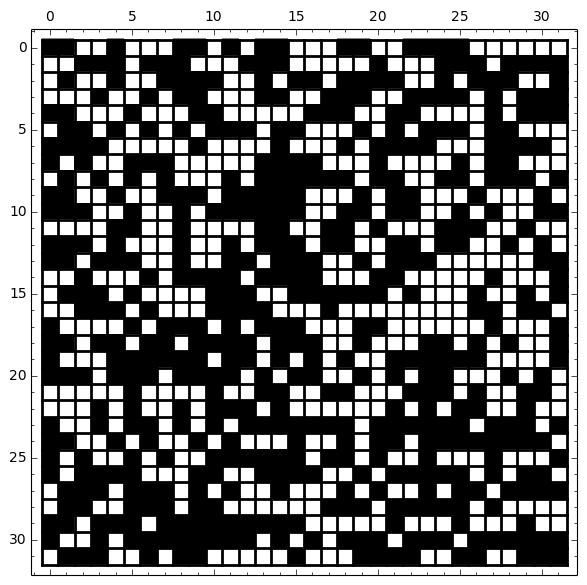
\includegraphics[scale=0.5]{figures/BC_lfsr_ex1.png}   %BERM0
\end{center}
\caption{Visualisierung der pseudozuf�lligen Bitfolge aus Abbildung~\ref{Sage-code-bool-psr},
   erzeugt mit dem SageMath-Beispiel~\ref{Sage-code-bool-psr}
   (1 = schwarz, 0 = wei�)}\label{fig-bool-lfsr2}
\end{figure}
\clearpage

\subsection{Algebraischer Angriff \index{algebraischer Angriff}\index{Angriff!algebraisch}
            auf lineare Schieberegister}\label{ss-bool-alg2}

Auch einfache Zufallsgeneratoren\index{Zufallsgenerator} wie die linearen
Schieberegister\index{lineares Schieberegister}\index{Schieberegister!linear} liefern,
wie gesehen, Bitfolgen, die mit statistischen Mitteln nicht ohne weiteres
von "`echtem"' Zufall unterschieden werden k�nnen und f�r statistische
Methoden der Kryptoanalyse keinen unmittelbar erfolgversprechenden
Ansatz bieten. Anders sieht es aus, wenn man
bekannten Klartext\index{bekannter Klartext}\index{Klartext!bekannt} annimmt
-- dann erh�lt man Gleichungen f�r die Schl�sselbits. Werden die
Schl�sselbits nach einem einfachen Algorithmus erzeugt, kann man
mit algebraischer
Kryptoanalyse\index{algebraische Kryptoanalyse}\index{Kryptoanalyse!algebraisch},
d.\,h. durch Aufl�sung dieser Gleichungen, auf Erfolg hoffen. Dies ist besonders
f�r lineare Schieberegister\footnote{%
  Die "`R�ckkopplung"' wird in der Bezeichnungsweise meistens weggelassen,
  wenn keine Missverst�ndnisse zu bef�rchten sind, ist hier aber implizit
  immer mit gemeint.
} der Fall.

Nehmen wir an, ein lineares
Schieberegister\index{lineares Schieberegister}\index{Schieberegister!linear}
hat den Schl�sselbitstrom $u_0, u_1, \ldots$ nach den
Formeln~(\ref{eq-bool-lfsr1}) und (\ref{eq-bool-lfsr2}) erzeugt.
Mit diesem Schl�sselstrom\index{Schl�sselstrom} wurde ein
Klartext $a$ per XOR\index{XOR}\index{Verschl�sselung!XOR}
zum Geheimtext $c$ verschl�sselt, $c_i = a_i + u_i$
f�r $i = 0, 1, \ldots$ Was kann die Gegnerin erreichen, wenn sie ein
St�ck vom Anfang des Klartexts kennt?

Nun, kennt sie die ersten $l+1$ Bits des Klartexts, so hat sie sofort
die entsprechenden Bits $u_0, \ldots, u_l$ des Schl�sselstroms,
insbesondere den Startwert. F�r die noch unbekannten Koeffizienten
$s_i$ kennt sie eine lineare Relation:
\[
     s_1 u_{l-1} + \cdots + s_l u_0 = u_l.
\]
Jedes weitere bekannte Bit des Klartexts liefert eine weitere Relation,
und mit $l$ solchen Relationen, also insgesamt $2l$ Bits an bekanntem
Klartext, liefert die sehr einfache Lineare
Algebra\index{lineare Algebra}\index{Algebra!lineare} �ber dem K�rper
$\F_2$ im allgemeinen eine eindeutige L�sung. Die
$l \times l$-Koeffizientenmatrix dieses linearen
Gleichungssystems\index{lineares Gleichungssystem}\index{Gleichungssystem!linear}
ist im Wesentlichen die Matrix $U$ des n�chsten Abschnitts. Ein
kleiner Umweg macht die L�sung noch ein wenig eleganter -- in den n�chsten,
etwas mehr Mathematik voraussetzenden Abschnitten wird bewiesen:

\begin{satz}\label{thm-bool-lfsr}
  Ein lineares Schieberegister\index{lineares Schieberegister}\index{Schieberegister!linear}
  der L�nge $l$ ist aus den ersten $2l$ Bits
  vorhersagbar. Der Aufwand dazu betr�gt ungef�hr $\frac{1}{3} \cdot l^3$
  Bitoperationen.
\end{satz}

\subsubsection*{Vorhersage linearer Schieberegister}

Nehmen wir an, wir kennen die ersten $2l$ Bits $u_0, \ldots, u_{2l-1}$
aus einem linearen Schieberegister\index{lineares Schieberegister}\index{Schieberegister!linear}
der L�nge $l$. Die Lineare Algebra l�sst
sich eleganter formulieren, wenn man die {\bf Zustandsvektoren\index{Zustandsvektor}}
\[
     u_{(i)} = (u_i, \ldots, u_{i+l-1}) \quad \text{f�r } i = 0, 1, \ldots
\]
verwendet. Dabei ist $u_{(i)}$ gerade der Inhalt des Registers beim Schritt
Nummer $i$ (in umgekehrter Reihenfolge) -- d.\,h., die Analyse konzentriert
sich nicht auf den Output, sondern setzt bei den Zust�nden an. Die
Rekursionsformel~(\ref{eq-bool-lfsr1}) kann man dann f�r $n \geq l$ in
Matrixform als
\[
     \begin{pmatrix} u_{n-l+1} \\ \vdots \\ u_{n-1} \\ u_{n} \end{pmatrix}
     =
     \begin{pmatrix} 0      & 1      & \ldots & 0      \\
                     \vdots & \vdots & \ddots & \vdots \\
                     0      & 0      & \ldots & 1      \\
                     s_l    & s_{l-1}    & \ldots & s_1 \end{pmatrix}
     \begin{pmatrix} u_{n-l} \\ \vdots \\ u_{n-2} \\ u_{n-1} \end{pmatrix}
\]
schreiben oder sehr knapp und �bersichtlich in der Form (mit substituierten Indizes
$m = n-l+1$)
\[
     u_{(m)} = S \cdot u_{(m-1)} \quad \text{f�r } m \geq 1\,,
\]
wobei $S$ die Koeffizientenmatrix ist. Noch einen Schritt weiter gehend
fasst man $l$ aufeinanderfolgende Zustandsvektoren
$u_{(i)}, \ldots, u_{(i+l-1)}$ zu einer Zustandsmatrix
\[
     U_{(i)} = \begin{pmatrix} u_i      & u_{i+1}      & \ldots & u_{i+l-1}      \\
                               u_{i+1} & u_{i+2} & \ldots & u_{i+l} \\
                               \vdots  & \vdots & \ddots & \vdots     \\
                     u_{i+l-1}    & u_{i+l} & \ldots & u_{2l-2} \end{pmatrix}
\]
zusammen, setzt $U = U_{(0)}$, $V = U_{(1)}$, und erh�lt damit die Formel
\[
     V  =  S \cdot U,
\]
die die unbekannten Koeffizienten $s_1, \ldots, s_l$ durch die bekannten
Klartextbits $u_0, \ldots, u_{2l-1}$ ausdr�ckt. Vor allem aber gestattet sie,
als Lohn f�r die Bem�hungen sofort die L�sung hinzuschreiben -- vorausgesetzt,
die Matrix $U$ ist invertierbar:
\[
     S  =  V \cdot U^{-1},
\]
denn aus der Matrix $S$ kann man ja die Koeffizienten $s_j$ auslesen.
Mehr zur Invertierbarkeit sp�ter.

\subsubsection*{Beispiel}

Wir haben einen Geheimtext vorliegen:
\begin{verbatim}
   10011100 10100100 01010110 10100110 01011101 10101110
   01100101 10000000 00111011 10000010 11011001 11010111
   00110010 11111110 01010011 10000010 10101100 00010010
   11000110 01010101 00001011 11010011 01111011 10110000
   10011111 00100100 00001111 01010011 11111101
\end{verbatim}
Wir vermuten, dass er XOR-chiffriert\index{XOR}\index{Verschl�sselung!XOR}
ist mit einem Schl�sselstrom, der
durch ein lineares Schieberegister der L�nge $l = 16$ erzeugt wurde.
Der Kontext l�sst vermuten, dass der Text mit dem Wort "`Treffpunkt"'
beginnt. Zum Brechen ben�tigen wir nach der Theorie 32 Bits, also
nur die ersten vier Buchstaben. Daraus ermitteln wir 32 Bits des
Schl�sselstroms:
\begin{verbatim}
    01010100 01110010 01100101 01100110 = T r e f
    10011100 10100100 01010110 10100110   cipher bits
    -------- -------- -------- --------
    11001000 11010110 00110011 11000000   key bits
\end{verbatim}
Im SageMath-Beispiel~\ref{Sage-code-bool-lfsr2} wird die Koeffizientenmatrix
bestimmt. Die letzte Zeile sagt uns, dass die $s_i = 0$ sind au�er
$s_{16} = s_5 = s_3 = s_2 = 1$.

Damit kennen wir das Schieberegister und den Startwert, k�nnen den
gesamten Schl�sselstrom berechnen -- ja, es ist der aus Abbildung~\ref{Sage-code-bool-psr}
-- und damit den Klartext herstellen
(der �brigens nicht ganz so beginnt wie vermutet).

\begin{sagecode}
\begin{verbatim}

sage: l = 16
sage: kbits =
      [1,1,0,0,1,0,0,0,1,1,0,1,0,1,1,0,0,0,1,1,0,0,1,1,1,1,0,0,0,0,0,0]
sage: ulist = []
sage: for i in range(0,l):
        state = kbits[i:(l+i)]
        ulist.append(state)
sage: U = matrix(GF(2),ulist)
sage: det(U)
1
sage: W = U.inverse()
sage: vlist = []
sage: for i in range(1,l+1):
        state = kbits[i:(l+i)]
        vlist.append(state)
sage: V = matrix(GF(2),vlist)
sage: S = V*W
sage: S
[0 1 0 0 0 0 0 0 0 0 0 0 0 0 0 0]
[0 0 1 0 0 0 0 0 0 0 0 0 0 0 0 0]
[0 0 0 1 0 0 0 0 0 0 0 0 0 0 0 0]
[0 0 0 0 1 0 0 0 0 0 0 0 0 0 0 0]
[0 0 0 0 0 1 0 0 0 0 0 0 0 0 0 0]
[0 0 0 0 0 0 1 0 0 0 0 0 0 0 0 0]
[0 0 0 0 0 0 0 1 0 0 0 0 0 0 0 0]
[0 0 0 0 0 0 0 0 1 0 0 0 0 0 0 0]
[0 0 0 0 0 0 0 0 0 1 0 0 0 0 0 0]
[0 0 0 0 0 0 0 0 0 0 1 0 0 0 0 0]
[0 0 0 0 0 0 0 0 0 0 0 1 0 0 0 0]
[0 0 0 0 0 0 0 0 0 0 0 0 1 0 0 0]
[0 0 0 0 0 0 0 0 0 0 0 0 0 1 0 0]
[0 0 0 0 0 0 0 0 0 0 0 0 0 0 1 0]
[0 0 0 0 0 0 0 0 0 0 0 0 0 0 0 1]
[1 0 0 0 0 0 0 0 0 0 0 1 0 1 1 0]
\end{verbatim}
\caption{Bestimmung einer Koeffizientenmatrix}\label{Sage-code-bool-lfsr2}
\end{sagecode}

\subsubsection*{Beweis des Satzes}

F�r den Fall, dass die Zustandsmatrix $U = U_{(0)}$ invertierbar ist,
haben wir oben schon gezeigt, dass die Koeffizienten eindeutig bestimmbar sind.
Insbesondere ist dann das Schieberegister bekannt und aller weitere Output
vorhersagbar. Wir m�ssen uns also noch mit der M�glichkeit auseinandersetzen,
dass die Matrix $U$ nicht invertierbar sein k�nnte.

Falls einer der ersten $l$ Zustandsvektoren (= Zeilen der Matrix $U$)
Null ist, sind auch alle weiteren Null, die Vorhersage ist also trivial.

Wir k�nnen also annehmen, dass diese Vektoren alle nicht Null, aber linear
abh�ngig sind. Dann gibt es einen kleinsten Index $k \geq 1$, so dass
$u_{(k)}$ in dem von $u_{(0)}, \ldots, u_{(k-1)}$ aufgespannten
Unterraum liegt. D.\,h., es gibt Koeffizienten $t_1, \ldots, t_k \in \F_2$ mit
\[
     u_{(k)}  =  t_1 u_{(k-1)} + \cdots + t_k u_{(0)}.
\]
Dann gilt aber auch $u_{(k+1)} = S\cdot u_{(k)} =
t_1 S\cdot u_{(k-1)} + \cdots + t_k S\cdot u_{(0)} =
t_1 u_{(k)} + \cdots + t_k u_{(1)}$ und weiter durch Induktion
\[
     u_{(n)}  =  t_1 u_{(n-1)} + \cdots + t_k u_{(n-k)}
     \quad \text{f�r alle } n \geq k.
\]
Durch diese Formel werden also auch alle weiteren Bits vorhergesagt.

Die Aussage �ber den Aufwand folgt aus Satz~\ref{thm-bool-lin}.

\begin{description}
   \item[Diskussion:] ~
      \begin{itemize}
         \item Diese �berlegung ergibt f�r den Fall einer nicht invertierbaren
            Zustandsmatrix ein k�rzeres lineares Schieberegisters (der L�nge
            $k < l$), das die gleiche Folge erzeugt. In diesem Fall werden
            die Koeffizienten des originalen Registers also nicht bestimmt,
            aber die weitere Folge trotzdem korrekt vorhergesagt.
         \item Wenn nicht die ersten Bits, sondern $2l$ zusammenh�ngende
            Bits an sp�terer Stelle bekannt sind, ergibt der Satz zun�chst
            nur eine Berechnung der sp�teren Bits. Im Regelfall, wo die
            Zustandsmatrix $U$ invertierbar ist, ist das Register aber
            dann v�llig bekannt und kann nat�rlich auch r�ckw�rts zur
            Bestimmung der Vorg�ngerbits eingesetzt werden. Ist die
            Zustandsmatrix nicht invertierbar, kann man das gleiche mit dem
            eben konstruierten k�rzeren linearen Schieberegister erreichen.
         \item Etwas komplizierter wird die Situation, wenn man zwar $2l$
            Bits des Schl�sselstroms kennt, diese aber nicht zusammenh�ngen.
            Auch dann erh�lt man lineare Relationen, in denen aber
            zus�tzlich unbekannte Zwischenbits vorkommen. Ist $m$ die Zahl
            der L�cken, so hat man dann insgesamt $l+m$ lineare Gleichungen
            f�r $l+m$ unbekannte Bits.
         \item Was aber, wenn auch die L�nge $l$ des Registers unbekannt ist?
            Das Durchprobieren aller Werte $l = 1, 2, 3, \ldots$ ist sicher
            l�stig, aber machbar. Es gibt aber auch den Algorithmus von
            Berlekamp-Massey\footnote{%
            in SageMath als {\tt sage.crypto.lfsr.berlekamp\_massey} enthalten,
            in CrypTool\,2 unter
            "`Kryptoanalyse"'/"`Generisch"'/"`Berlekamp-Massey-Algorithmus"'
            zu finden
            }, der ohne vorherige Kenntnis
            von $l$ sehr effizient ist. Dessen Behandlung w�rde aber hier
            zu weit f�hren.
      \end{itemize}
\end{description}

\subsubsection*{Fazit}

Kryptoanalyse bedeutet f�r Zufallsgeneratoren\index{Zufallsgenerator} wie in Abbildung~\ref{fig-bool-prg},
aus einem Teil ihres Outputs eine der folgenden Informationen zu bestimmen:
\begin{itemize}
\item die geheimen Parameter,
\item den Startwert,
\item weitere Teile des Outputs ("`Vorhersageproblem\index{Vorhersageproblem}"').
\end{itemize}
Wie wir bei den linearen
Schieberegistern\index{lineares Schieberegister}\index{Schieberegister!linear}
gesehen haben, ist es
realistisch, das Vorhersageproblem anzugehen, das auch l�sbar sein
kann, wenn die Bestimmung der internen Parameter nicht gelingt.
Wir halten fest:
\begin{quote}
   {\em Die Kryptoanalyse eines Zufallsgenerators bedeutet in erster Linie
   die L�sung des Vorhersageproblems. Ein Zufallsgenerator\index{Zufallsgenerator}
   ist kryptographisch
   sicher, wenn sein Vorhersageproblem nicht effizient l�sbar ist.}
\end{quote}

\begin{quote}
   {\em Lineare Schieberegister\index{lineares Schieberegister}\index{Schieberegister!linear}
   sind kryptographisch nicht sicher.}
\end{quote}

\subsection{Nichtlinearit�t\index{Nichtlinearit�t} f�r Schieberegister
   -- Ans�tze}\label{ss-bool-nlsr}

Lineare Schieberegister sind beliebt -- vor allem bei Elektro-Ingenieuren
und beim Milit�r -- denn sie sind
\begin{itemize}
	\item sehr einfach zu realisieren,
	\item extrem effizient in Hardware,
	\item als Zufallsgeneratoren f�r statistische Zwecke sehr gut geeignet,
	\item problemlos in gro�er Anzahl parallel zu betreiben,
	\item aber leider kryptologisch v�llig unsicher.
\end{itemize}
Um die positiven Eigenschaften zu nutzen und die kryptologische Schw�che
zu vermeiden, gibt es verschiedene Ans�tze.

\subsubsection*{Ansatz 1: Nichtlineare R�ckkopplung}

Die nichtlineare R�ckkopplung\index{R�ckkopplung}
folgt dem Schema aus Abbildung~\ref{fig-bool-fsr}
mit einer nichtlinearen Booleschen Funktion\index{Boolesche
Funktion}\index{Funktion!Boolesche} $f$.
Sie wird hier nicht weiter behandelt; ein ganz
einfaches, kryptographisch ungeeignetes Beispiel war das
SageMath-Beispiel~\ref{Sage-code-bool-fsr1}. Man kann aber auch
allgemein zeigen, dass solche nichtlinearen Schieberegister
(nonlinear feedback, NLFSR\footnote{%
   f�r Non-Linear Feedback Shift Register\index{Schieberegister!nichtlinear}
}
), f�r sich allein genommen, unter realistischen Annahmen
im praktischen Einsatz nicht kryptographisch
sicher sind \cite{Pom2016}.


\subsubsection*{Ansatz 2: Nichtlinearer Ausgabefilter}

Der nichtlineare Ausgabefilter\index{Ausgabefilter}
(Non-Linear Feedforward) folgt dem Schema
aus Abbildung~\ref{fig-bool-nlf}.
Das Schieberegister selbst ist linear. Der nichtlineare Ausgabefilter
ist ein Spezialfall des n�chsten Ansatzes.

\begin{figure}
\begin{center}
\begin{picture}(320,150)
  \linethickness{2pt}
  \put(20,20){\line(1,0){260}}
  \put(20,20){\line(0,1){30}}
  \put(20,50){\line(1,0){260}}
  \put(280,20){\line(0,1){30}}
  \put(260,120){\circle{30}}
  \put(256,117){$f$}

  \linethickness{1pt}
  \put(60,20){\line(0,1){30}}
  \put(100,20){\line(0,1){30}}
  \put(240,20){\line(0,1){30}}
  \put(200,20){\line(0,1){30}}
  \put(110,30){\ldots}
  \put(180,30){\ldots}

  \put(40,20){\line(0,-1){20}}
  \put(80,20){\line(0,-1){20}}
  \put(220,20){\line(0,-1){20}}
  \put(260,20){\line(0,-1){20}}
  \put(260,0){\line(-1,0){260}}
  \put(0,0){\line(0,1){35}}
  \put(0,35){\vector(1,0){20}}

  \put(260,50){\vector(0,1){53}}
  \put(220,50){\vector(1,2){29}}
  \put(80,50){\line(0,1){25}}
  \put(80,75){\vector(4,1){163}}
  \put(40,50){\line(0,1){70}}
  \put(40,120){\vector(1,0){203}}

  \put(277,120){\vector(1,0){43}}
\end{picture}
\end{center}
\caption{Nichtlinearer Ausgabefilter f�r ein lineares Schieberegister}\label{fig-bool-nlf}
\end{figure}

\subsubsection*{Ansatz 3: Nichtlinearer Kombinierer\index{Kombinierer}}

Hier wird eine "`Batterie"' aus $n$ linearen Schieberegistern -- die durchaus
unterschiedliche L�nge haben k�nnen und sollen -- parallel betrieben.
Ihre Outputfolgen werden in eine
Boolesche Funktion\index{Boolesche Funktion}\index{Funktion!Boolesche}
$f\!\!: \F_2^n \longrightarrow \F_2$ gef�ttert\footnote{%
   daher auch hierf�r gelegentlich die Bezeichnung Non-Linear Feedforward
}, siehe Abbildung~\ref{fig-bool-nlc}.
Ein Ansatz zur Analyse dieses Verfahrens folgt in Abschnitt~\ref{ss-bool-bsana}.

\begin{figure}
\begin{center}
\begin{picture}(350,200)
  \linethickness{2pt}
  \put(20,20){\line(1,0){260}}
  \put(20,20){\line(0,1){30}}
  \put(20,50){\line(1,0){260}}
  \put(280,20){\line(0,1){30}}

  \linethickness{1pt}
  \put(60,20){\line(0,1){30}}
  \put(100,20){\line(0,1){30}}
  \put(240,20){\line(0,1){30}}
  \put(200,20){\line(0,1){30}}
  \put(110,30){\ldots}
  \put(180,30){\ldots}

  \put(40,20){\line(0,-1){20}}
  \put(80,20){\line(0,-1){20}}
  \put(220,20){\line(0,-1){20}}
  \put(260,20){\line(0,-1){20}}
  \put(260,0){\line(-1,0){260}}
  \put(0,0){\line(0,1){35}}
  \put(0,35){\vector(1,0){20}}

  \linethickness{2pt}
  \put(20,150){\line(1,0){260}}
  \put(20,150){\line(0,1){30}}
  \put(20,180){\line(1,0){260}}
  \put(280,150){\line(0,1){30}}

  \linethickness{1pt}
  \put(60,150){\line(0,1){30}}
  \put(100,150){\line(0,1){30}}
  \put(240,150){\line(0,1){30}}
  \put(200,150){\line(0,1){30}}
  \put(110,160){\ldots}
  \put(180,160){\ldots}

  \put(40,150){\line(0,-1){20}}
  \put(80,150){\line(0,-1){20}}
  \put(220,150){\line(0,-1){20}}
  \put(260,150){\line(0,-1){20}}
  \put(260,130){\line(-1,0){260}}
  \put(0,130){\line(0,1){35}}
  \put(0,165){\vector(1,0){20}}

  \put(80,100){$\vdots$}
  \put(220,100){$\vdots$}
  \put(80,70){$\vdots$}
  \put(220,70){$\vdots$}

  \put(280,165){\vector(1,0){20}}
  \put(280,35){\vector(1,0){20}}
  \put(315,100){\oval(30,160)}
  \put(330,100){\vector(1,0){20}}
  \put(313,97){$f$}
\end{picture}
\end{center}
\caption{Nichtlinearer Kombinierer}\label{fig-bool-nlc}
\end{figure}

\subsubsection*{Ansatz 4: Auswahlsteuerung/Dezimierung/Taktung}

Weitere M�glichkeiten bestehen in verschiedenen Methoden zur Steuerung
einer Batterie von $n$ parallel betriebenen linearen Schieberegistern
durch ein weiteres lineares Schieberegister:
\begin{itemize}
	\item Bei der {\bf Auswahlsteuerung}\index{Auswahlsteuerung}
        wird je nach Zustand des "`Hilfsregisters"'
	   das aktuelle Output-Bit von genau einem der "`Batterie-Register"' als
	   Output des Zufallsgenerators ausgew�hlt. Allgemeiner kann man auch
	   eine Auswahl "`$r$ aus $n$"' treffen.
	\item Bei der {\bf Dezimierung}\index{Dezimierung} nimmt man
        im allgemeinen $n = 1$ an und gibt das
	   Output-Bit des einen Batterie-Registers nur dann aus, wenn das
	   Hilfsregister einen bestimmten Zustand hat. Diese Art der Dezimierung
	   kann man nat�rlich analog auf jede Bitfolge anwenden.
	\item Bei der {\bf Taktung}\index{Taktung} gibt der Zustand
        des Hilfsregisters an, welche
	   der Batterie-Register im aktuellen Taktzyklus weitergeschoben werden
	   (und um wieviele Positionen) und welche in ihrem momentanen Zustand bleiben.
	   Das ist vergleichbar mit der Steuerlogik von
        Rotor-Maschinen\index{Rotor-Maschine}.
\end{itemize}
Diese Ans�tze lassen sich oft bequem auch als nichtlineare Kombinierer schreiben,
so dass Ansatz 3 als der g�ngigste Ansatz zur Rettung der linearen
Schieberegister\index{lineares Schieberegister}\index{Schieberegister!linear}
angesehen werden kann.

Der Mobilfunk-Verschl�sselungsstandard
\href{http://de.wikipedia.org/wiki/A5\_(Algorithmus)}{A5/1}\index{A5} verwendet
drei leicht unterschiedlich getaktete lineare Schieberegister der L�ngen
19, 22 und 23 mit jeweils maximaler Periode, deren
Outputstr�me linear (n�mlich einfach durch bin�re Addition)
kombiniert werden. Bei A5/2 -- das noch schw�cher ist -- wird
die Taktung durch ein Hilfsregister geregelt. Beide Varianten
lassen sich auf handels�blichen PCs in Echtzeit brechen.

Der Bluetooth-Verschl�sselungsstandard $\mathrm{E}_0$\index{E0} verwendet vier
lineare Schieberegister, die nichtlinear kombiniert werden. Dieses Verfahren
ist etwas st�rker als A5, aber auch zu schwach f�r echte Sicherheit \cite{Schm2016}.

\subsubsection*{Beispiel: Der Geffe-Generator}

Das einfachste Beispiel f�r die Auswahlsteuerung ist der
Geffe-Generator\index{Geffe-Generator},
der durch das Schema in Abbildung~\ref{fig-bool-gef}
beschrieben wird. Die Ausgabe ist $x$, wenn $z = 0$, und $y$, wenn
$z = 1$. Das kann man so als Formel ausdr�cken:
\begin{eqnarray*}
   u & = & \begin{cases}
              x, & \text{wenn } z = 0, \\
              y, & \text{wenn } z = 1
           \end{cases} \\
      & = & (1 - z) x + zy = x + zx + zy.
\end{eqnarray*}
Also l�sst sich der Geffe-Generator auch durch einen nichtlinearen
Kombinierer mit einer Booleschen Funktion
$f\!\!: \F_2^3 \longrightarrow \F_2$ vom Grad 2 beschreiben. Diese
wird zur sp�teren Verwendung im SageMath-Beispiel~\ref{Sage-code-bool-gef}
erzeugt.

\begin{figure}
\begin{center}
\setlength{\unitlength}{1pt}
\begin{picture}(350,200)
  \linethickness{2pt}
  \put(20,20){\line(1,0){260}}
  \put(20,20){\line(0,1){30}}
  \put(20,50){\line(1,0){260}}
  \put(280,20){\line(0,1){30}}

  \linethickness{1pt}
  \put(60,20){\line(0,1){30}}
  \put(100,20){\line(0,1){30}}
  \put(240,20){\line(0,1){30}}
  \put(200,20){\line(0,1){30}}
  \put(110,30){\ldots}
  \put(180,30){\ldots}

  \put(40,20){\line(0,-1){20}}
  \put(80,20){\line(0,-1){20}}
  \put(220,20){\line(0,-1){20}}
  \put(260,20){\line(0,-1){20}}
  \put(260,0){\line(-1,0){260}}
  \put(0,0){\line(0,1){35}}
  \put(0,35){\vector(1,0){20}}

  \linethickness{2pt}
  \put(20,80){\line(1,0){260}}
  \put(20,80){\line(0,1){30}}
  \put(20,110){\line(1,0){260}}
  \put(280,80){\line(0,1){30}}

  \linethickness{1pt}
  \put(60,80){\line(0,1){30}}
  \put(100,80){\line(0,1){30}}
  \put(240,80){\line(0,1){30}}
  \put(200,80){\line(0,1){30}}
  \put(110,90){\ldots}
  \put(180,90){\ldots}

  \put(40,80){\line(0,-1){20}}
  \put(80,80){\line(0,-1){20}}
  \put(220,80){\line(0,-1){20}}
  \put(260,80){\line(0,-1){20}}
  \put(260,60){\line(-1,0){260}}
  \put(0,60){\line(0,1){35}}
  \put(0,95){\vector(1,0){20}}

  \linethickness{2pt}
  \put(50,160){\line(1,0){260}}
  \put(50,160){\line(0,1){30}}
  \put(50,190){\line(1,0){260}}
  \put(310,160){\line(0,1){30}}

  \linethickness{1pt}
  \put(90,160){\line(0,1){30}}
  \put(130,160){\line(0,1){30}}
  \put(270,160){\line(0,1){30}}
  \put(230,160){\line(0,1){30}}
  \put(140,170){\ldots}
  \put(210,170){\ldots}

  \put(70,160){\line(0,-1){20}}
  \put(110,160){\line(0,-1){20}}
  \put(250,160){\line(0,-1){20}}
  \put(290,160){\line(0,-1){20}}
  \put(290,140){\line(-1,0){260}}
  \put(30,140){\line(0,1){35}}
  \put(30,175){\vector(1,0){20}}

  \put(310,175){\line(1,0){20}}
  \put(330,175){\line(0,-1){40}}
  \put(333,152){$z$}
  \put(330,135){\line(-1,0){15}}
  \put(315,135){\vector(0,-1){25}}

  \put(280,95){\vector(1,0){20}}
  \put(288,97){$x$}
  \put(280,35){\vector(1,0){20}}
  \put(288,38){$y$}
  \put(315,65){\oval(30,90)}
  \put(330,65){\line(-1,-1){30}}
  \put(330,65){\vector(1,0){20}}
\end{picture}
\end{center}
\caption{Geffe-Generator}\label{fig-bool-gef}
\end{figure}

\begin{sagecode}
\begin{verbatim}

sage: geff = BoolF(str2bbl("00011100"),method="ANF")
sage: geff.printTT()
Value at 000 is 0
Value at 001 is 0
Value at 010 is 0
Value at 011 is 1
Value at 100 is 1
Value at 101 is 0
Value at 110 is 1
Value at 111 is 1
\end{verbatim}
\caption{Die Geffe-Funktion}\label{Sage-code-bool-gef}
\end{sagecode}

\subsection{Implementation eines nichtlinearen Kombinierers}\label{ss-bool-ncsr}

Ein nichtlinearer Kombinierer\index{Kombinierer} ben�tigt mehrere parallel betriebene
lineare Schieberegister. Dies legt nahe, diese als Objekte zu
implementieren, d.\,h., eine Klasse {\tt LFSR} zu definieren\footnote{%
   siehe auch in CrypTool\,2 unter "`Protokolle"'/"`LFSR"' bzw. "`NLFSR"'
}.

\begin{description}
   \item[Klasse {\tt LSFR}:] ~
      \begin{description}
         \item[Attribute:] ~
            \begin{itemize}
               \item {\tt length}: die L�nge des Registers
               \item {\tt taplist}: die Liste der Koeffizienten ("`Taps"'\footnote{%
                    auf deutsch etwa "`Abzweig"' oder "`Abgriff"', weil bei einer
                    Hardware-Implementierung genau an diesen Stellen die f�r die
                    R�ckkopplung verwendeten Bits abgegriffen werden
                  }), die die  r�ckzukoppelnden Bits definieren (konstant)
               \item {\tt state}: der Zustand des Registers (ver�nderbar)
            \end{itemize}
         \item[Methoden:] ~
            \begin{itemize}
               \item {\tt setLength}: Definition der L�nge (nur implizit bei
                  der Initialisierung verwendet)
               \item {\tt setTaps}: Besetzung der Tap- (= Koeffizienten-) Liste
                  (nur implizit bei der Initialisierung verwendet)
               \item {\tt setState}: Belegung des Registers mit einem Zustand
               \item {\tt getLength}: Ausgabe der L�nge
               \item {\tt nextBits}: Erzeugung einer vorgegebenen Anzahl von
                  Ausgabebits und kontinuierliche Weiterschaltung des Zustands
            \end{itemize}
      \end{description}
\end{description}
Dazu ist es zur �berwachung des Registers praktisch, noch eine Methode
(die in Python\index{Python} generisch {\tt \_\_str\_\_} hei�t) zu haben, die die
Attribute in lesbarer Form ausgibt.

F�r die Implementation siehe das SageMath-Beispiel~\ref{Sage-code-bool-lfsr3}
im Abschnitt~\ref{ss-bool-lfsrclass}.

\subsubsection*{Beispiel: Geffe-Generator\index{Geffe-Generator}}

Zun�chst w�hlen wir drei lineare Schieberegister der L�ngen 15, 16 und 17,
deren Perioden\footnote{%
  nach den Listen primitiver Polynome in \cite{Menezes2001}
} $2^{15} - 1 = 32767$, $2^{16} - 1 = 65535$ und
$2^{17} - 1 = 131071$ sind, und diese sind paarweise teilerfremd, siehe
SageMath-Beispiel~\ref{Sage-code-bool-per}.
Fasst man ihren Output in jedem Takt zu Bitbl�cken der L�nge $3$
zusammen, so hat diese Folge eine Periode der eindrucksvollen L�nge
$281459944554495$, also knapp $300 \times 10^{12}$ (300 Billionen\footnote{%
  europ�ische Billionen. Amerikanisch w�ren das 300 Trillionen.
}).
Die drei Register werden im SageMath-Beispiel~\ref{Sage-code-bool-regs}
definiert; die Rekursionsformel f�r das dritte davon, das
Steuerungsregister {\tt reg17}, ist z.\,B. $u_n = u_{n-3} + u_{n-17}$,
da genau die Taps 3 und 17 gesetzt sind.
Mit jedem von ihnen wird eine Folge der L�nge 100 erzeugt,
siehe SageMath-Beispiel~\ref{Sage-code-bool-seqs}. Diese werden im
SageMath-Beispiel~\ref{Sage-code-bool-gef-seq} mithilfe der
Geffe-Funktion kombiniert.

\begin{sagecode}
\begin{verbatim}

sage: n15 = 2**15 - 1; n15
32767
sage: n15.factor()
7 * 31 * 151
sage: n16 = 2**16 - 1; n16
65535
sage: n16.factor()
3 * 5 * 17 * 257
sage: n17 = 2**17 - 1; n17
131071
sage: n17.factor()
131071
sage: period = n15 * n16 * n17; period
281459944554495
\end{verbatim}
\caption{Eine Periodenberechnung}\label{Sage-code-bool-per}
\end{sagecode}

\begin{sagecode}
\begin{verbatim}

sage: reg15 = LFSR([1,0,0,0,0,0,0,0,0,0,0,0,0,0,1])
sage: reg15.setState([0,1,1,0,1,0,1,1,0,0,0,1,0,0,1])
sage: print(reg15)
Length: 15 | Taps: 100000000000001 | State: 011010110001001
sage: reg16 = LFSR([0,1,1,0,1,0,0,0,0,0,0,0,0,0,0,1])
sage: reg16.setState([0,1,1,0,1,0,1,1,0,0,0,1,0,0,1,1])
sage: print(reg16)
Length: 16 | Taps: 0110100000000001 | State: 0110101100010011
sage: reg17 = LFSR([0,0,1,0,0,0,0,0,0,0,0,0,0,0,0,0,1])
sage: reg17.setState([0,1,1,0,1,0,1,1,0,0,0,1,0,0,1,1,1])
sage: print(reg17)
Length: 17 | Taps: 00100000000000001 | State: 01101011000100111
\end{verbatim}
\caption{Drei lineare Schieberegister}\label{Sage-code-bool-regs}
\end{sagecode}

\begin{sagecode}
\begin{verbatim}

sage: nofBits = 100
sage: outlist15 = reg15.nextBits(nofBits)
sage: print(outlist15)
[1, 0, 0, 1, 0, 0, 0, 1, 1, 0, 1, 0, 1, 1, 0, 1, 1, 1, 0, 0,
 0, 0, 1, 0, 0, 1, 1, 0, 1, 1, 0, 1, 0, 0, 0, 0, 0, 1, 1, 1,
 0, 1, 1, 0, 1, 1, 0, 0, 0, 0, 0, 0, 1, 0, 1, 1, 0, 1, 1, 0,
 1, 1, 1, 1, 1, 1, 1, 0, 0, 1, 0, 0, 1, 0, 0, 1, 0, 1, 0, 1,
 0, 1, 1, 1, 0, 0, 0, 1, 1, 1, 0, 0, 1, 1, 0, 0, 1, 0, 1, 1]
sage: outlist16 = reg16.nextBits(nofBits)
sage: print(outlist16)
[1, 1, 0, 0, 1, 0, 0, 0, 1, 1, 0, 1, 0, 1, 1, 0, 0, 0, 1, 1,
 0, 0, 1, 1, 1, 1, 0, 0, 0, 0, 0, 0, 0, 0, 1, 1, 1, 0, 1, 1,
 1, 0, 0, 0, 1, 1, 1, 0, 0, 0, 0, 0, 1, 0, 0, 0, 1, 1, 1, 0,
 1, 1, 1, 1, 0, 1, 0, 0, 1, 0, 0, 1, 1, 1, 1, 0, 0, 1, 0, 1,
 1, 0, 1, 1, 1, 1, 0, 0, 1, 0, 1, 1, 1, 0, 0, 1, 0, 0, 0, 1]
sage: outlist17 = reg17.nextBits(nofBits)
sage: print(outlist17)
[1, 1, 1, 0, 0, 1, 0, 0, 0, 1, 1, 0, 1, 0, 1, 1, 0, 0, 0, 1,
 0, 0, 0, 0, 0, 0, 1, 1, 0, 0, 1, 1, 1, 1, 1, 1, 0, 1, 1, 0,
 1, 1, 0, 0, 0, 0, 0, 1, 1, 1, 0, 0, 0, 0, 1, 1, 0, 0, 0, 0,
 0, 0, 0, 0, 1, 1, 1, 1, 1, 1, 1, 0, 0, 1, 0, 0, 1, 0, 0, 1,
 0, 1, 0, 1, 0, 1, 0, 1, 1, 0, 0, 1, 0, 1, 1, 0, 0, 1, 1, 0]
\end{verbatim}
\caption{Drei LFSR-Folgen}\label{Sage-code-bool-seqs}
\end{sagecode}
\clearpage

\begin{sagecode}
\begin{verbatim}

sage: outlist = []
sage: for i in range(0,nofBits):
....:     x = [outlist15[i],outlist16[i],outlist17[i]]
....:     outlist.append(geff.valueAt(x))
....:
sage: print(outlist)
[1, 1, 0, 1, 0, 0, 0, 1, 1, 1, 0, 0, 0, 1, 1, 0, 1, 1, 0, 1,
 0, 0, 1, 0, 0, 1, 0, 0, 1, 1, 0, 0, 0, 0, 1, 1, 0, 0, 1, 1,
 1, 0, 1, 0, 1, 1, 0, 0, 0, 0, 0, 0, 1, 0, 0, 0, 0, 1, 1, 0,
 1, 1, 1, 1, 0, 1, 0, 0, 1, 0, 0, 0, 1, 1, 0, 1, 0, 1, 0, 1,
 0, 0, 1, 1, 0, 1, 0, 0, 1, 1, 0, 1, 1, 0, 0, 0, 1, 0, 0, 1]
\end{verbatim}
\caption{Die kombinierte Folge}\label{Sage-code-bool-gef-seq}
\end{sagecode}

\subsection{Korrelationsattacken\index{Korrelationsattacke}
    -- die Achillesferse der Kombinierer}\label{ss-bool-bsana}

Sei $f\!\!: \F_2^n \longrightarrow \F_2$ die Kombinierfunktion eines
nichtlinearen Kombinierers\index{Kombinierer}. Die Anzahl
\[
   K_f := \#\{ x = (x_1, \ldots, x_n) \in \F_2^n \:|\: f(x) = x_1 \}
\]
gibt an, wie oft der Funktionswert mit dem ersten Argument �bereinstimmt.
Ist sie $> 2^{n-1}$, so ist die Wahrscheinlichkeit f�r diese �bereinstimmung,
\[
   p = \frac{1}{2^n} \cdot K_f > \frac{1}{2},
\]
also �berdurchschnittlich. Die kombinierte Outputfolge "`korreliert"' also
st�rker mit dem Output des ersten linearen Schieberegisters, als zuf�llig
zu erwarten w�re. Ist $p < \frac{1}{2}$, so weicht die Korrelation nach
unten vom zuf�lligen Wert ab.

Diesen Effekt kann sich die Kryptoanalytikerin bei einem Angriff mit
bekanntem Klartext\index{bekannter Klartext}\index{Klartext!bekannt}
zunutze machen. Angenommen wird, dass ihr die
"`Hardware"', also die Rekursionsformeln f�r die Register (die Taps) und
auch die Kombinierfunktion $f$, bekannt ist. Gesucht sind die als Schl�ssel
betrachteten Startvektoren aller Register. Die Bits $k_0, \ldots, k_{r-1}$
des Schl�sselstroms\footnote{%
  der Einfachheit der Darstellung halber die ersten -- f�r irgendwelche $r$
  bekannten Schl�sselbits funktioniert die Argumentation genauso.
} seien bekannt. Mit einer Exhaustion �ber die $2^{l_1}$
Startvektoren des ersten Registers erzeugt man jedesmal die Folge
$u_0, \ldots, u_{r-1}$ und z�hlt die �bereinstimmungen. Zu erwarten ist
\[
   \frac{1}{r}\cdot \#\{i \:|\: u_i = k_i\} \approx
   \begin{cases}
      p & \text{beim richtigen Startvektor,} \\
      \frac{1}{2} & \text{sonst.}
   \end{cases}
\]
Falls $r$ gro� genug ist, kann man also den echten Startvektor des ersten
Registers mit einem Aufwand $\sim 2^{l_1}$ (mit hoher Wahrscheinlichkeit)
bestimmen. Macht man dann mit
den anderen Registern genauso weiter, gelingt die Identifikation des
gesamten Schl�ssels mit einem Aufwand $\sim 2^{l_1} + \cdots + 2^{l_n}$.
Das ist zwar exponenziell, aber wesentlich geringer als der Aufwand
$\sim 2^{l_1} \cdots 2^{l_n}$ f�r die naive vollst�ndige Schl�sselsuche.

In der Sprache der linearen
Kryptoanalyse\index{lineare Kryptoanalyse}\index{Kryptoanalyse!linear}
aus \ref{ss-bool-lka} haben
wir hier die lineare Relation\index{lineare Relation}\index{Relation!linear}
\[
     f(x_1, \ldots, x_n) \stackrel{p}{\approx} x_1
\]
f�r $f$ ausgenutzt. Klar ist, dass man analog jede lineare
Relation ausnutzen kann, um die Komplexit�t der vollst�ndigen Schl�sselsuche
zu reduzieren\footnote{%
  Eine genauere Analyse der Situation f�hrt auf den Begriff der
  Korrelationsimmunit�t\index{Korrelationsimmunit�t}, die mit dem linearen
  Potenzial\index{lineares Potenzial}\index{Potenzial!linear}
  verwandt ist.
}.

\subsubsection*{Korrelationen des Geffe-Generators}

F�r den Geffe-Generator\index{Geffe-Generator} kann man die Korrelationen aus
der Wahrheitstafel, Tabelle~\ref{tab-bool-gef-wt}, ablesen:
Als Wahrscheinlichkeit f�r die �bereinstimmung erh�lt man also
\[
   p = \begin{cases}
          \frac{3}{4} & \text{f�r das Register 1 ($x$),} \\
          \frac{3}{4} & \text{f�r das Register 2 ($y$),} \\
          \frac{1}{2} & \text{f�r das Register 3 ($z =$ Steuerung).}
       \end{cases}
\]
Daher lassen sich bei einer Korrelationsattacke die Startwerte f�r die
Register 1 und 2 -- die Batterieregister -- leicht schon aus kurzen
Outputfolgen bestimmen; den Startwert f�r Register 3, das Steuerungsregister,
findet man dann auch leicht durch Exhaustion.

\begin{table}
\begin{center}
  \begin{tabular}{|c|cccc|cccc|}\hline
      $x$    & $0$ & $0$ & $0$ & $0$ & $1$ & $1$ & $1$ & $1$ \\
      $y$    & $0$ & $0$ & $1$ & $1$ & $0$ & $0$ & $1$ & $1$ \\
      $z$    & $0$ & $1$ & $0$ & $1$ & $0$ & $1$ & $0$ & $1$ \\
    \hline
  $f(x,y,z)$ & $0$ & $0$ & $0$ & $1$ & $1$ & $0$ & $1$ & $1$ \\
    \hline
  \end{tabular}
\end{center}
\caption{Wahrheitstafel der Geffe-Funktion (waagerecht angeordnet)}\label{tab-bool-gef-wt}
\end{table}

Diese Schwachstelle des Geffe-Generators wird im
SageMath-Beispiel~\ref{Sage-code-bool-gef-lp} nachvollzogen, das als
Fortsetzung des SageMath-Beispiels~\ref{Sage-code-bool-gef} einzugeben ist.
Da wir das lineare Profil nur in der Klasse {\tt BoolMap} definiert
haben, m�ssen wir zuerst die Funktion {\tt geff} als Boolesche
Abbildung interpretieren -- also als Liste der L�nge 1 von Booleschen
Funktionen. Das lineare Profil wird als Matrix
mit 2 Spalten und 8 Zeilen gedacht. Die erste Spalte
{\tt [64, 0, 0, 0, 0, 0, 0, 0]} misst die �bereinstimmung mit der
Linearform 0 des Bildbereichs. Sie enth�lt also keine nennenswerte
Information, au�er dass alles durch $64$ zu dividieren ist. Die
zweite Spalte {\tt [0, 0, 16, 16, 16, 16, 0, 0]} wird
(nach dieser Division) in der Tabelle~\ref{tab-bool-gef-korr}
als Liste der Korrelationswahrscheinlichkeiten $p$ interpretiert.
Dabei wird die Formel
\[
     p = \frac{1}{2} \cdot (\pm \sqrt{\lambda} + 1)
\]
verwendet. Ist $\lambda = 0$, so $p = 1/2$. Ist  $\lambda = 1/4$,
so $p = 1/4$ oder $3/4$. Die Entscheidung zwischen diesen beiden
Werten f�r $p$ kann man anhand der Tabelle~\ref{tab-bool-gef-wt}
treffen.

\begin{table}
\begin{center}
\begin{tabular}{|l|cccccccc|} \hline
  Linearform     & $0$   &   $z$   &   $y$    &   $y+z$   &  $x$    &   $x+z$   &  $x+y$  & $x+y+z$ \\
  Repr�sentation & $000$ & $001$ & $010$ & $011$ & $100$ & $101$ & $110$ & $111$ \\ \hline
  Potenzial      & $0$   & $0$   & $1/4$ & $1/4$ & $1/4$ & $1/4$ & $0$   & $0$ \\
  Wahrsch. $p$   & $1/2$ & $1/2$ & $3/4$ & $1/4$ & $3/4$ & $3/4$ & $1/2$ & $1/2$ \\ \hline
\end{tabular}
\end{center}
\caption{Korrelationswahrscheinlichkeiten der Geffe-Funktion}\label{tab-bool-gef-korr}
\end{table}

\begin{sagecode}
\begin{verbatim}

sage: g = BoolMap([geff])
sage: linProf = g.linProf(); linProf
[[64, 0], [0, 0], [0, 16], [0, 16], [0, 16], [0, 16], [0, 0], [0, 0]]
\end{verbatim}
\caption{Lineares Profil der Geffe-Funktion}\label{Sage-code-bool-gef-lp}
\end{sagecode}

Im SageMath-Beispiel~\ref{Sage-code-bool-gef-coi} wird diese Erkenntnis auf
die mit dem Geffe-Generator erzeugte Folge der L�nge $100$ angewendet.
Zur Z�hlung der Koinzidenzen (= �bereinstimmungen) wird die Funktion {\tt coinc} aus dem
SageMath-Beispiel~\ref{Sage-code-bool-div-bbl} (im Anhang) verwendet. Mit dem ersten
Register gibt es $73$, mit dem zweiten $76$ Koinzidenzen, mit dem
dritten dagegen nur $41$. Das passt sehr gut zu den im Rahmen statistischer Schwankungen
theoretisch erwarteten Werten $75$, $75$, $50$.

\begin{sagecode}
\begin{verbatim}

sage: coinc(outlist15,outlist)
73
sage: coinc(outlist16,outlist)
76
sage: coinc(outlist17,outlist)
41
\end{verbatim}
\caption{Koinzidenzen des Geffe-Generators}\label{Sage-code-bool-gef-coi}
\end{sagecode}

\subsubsection*{Analyse des Geffe-Generators\index{Geffe-Generator}}

Diese deutlichen Ergebnisse legen nahe, dass die Analyse der beispielhaft
erzeugten Folge leicht sein sollte. F�r eine grobe Erfolgsabsch�tzung
kann man auf mathematische Strenge verzichten.

Betrachtet wird ein fest vorgegebener Bitblock $b \in \F_2^r$. Wir fragen
zun�chst, wie gro� die Wahrscheinlichkeit f�r einen zuf�lligen Bitblock
$u \in \F_2^r$ ist, an genau $t$ Stellen mit $b$ �bereinzustimmen,
also $t$ Koinzidenzen zu haben. Das ist genau die Fragestellung der
symmetrischen Binomialverteilung\index{Binomialverteilung}
(also mit $p = \frac{1}{2}$ als
Wahrscheinlichkeit einer einzelnen �bereinstimmung): Die
Wahrscheinlichkeit f�r genau $t$ Koinzidenzen ist
\[
     B_{r,\frac{1}{2}}(t)  =  \frac{\binom{r}{t}}{2^r}.
\]
Die Wahrscheinlichkeit f�r bis zu $T$ Koinzidenzen ist also
\[
     \sum_{t=0}^T B_{r,\frac{1}{2}}(t)
       =  \frac{1}{2^r} \cdot \sum_{t=0}^T \binom{r}{t}.
\]
Wenn $r$ nicht zu gro� ist, kann man diesen Wert f�r eine konkrete
Schranke $T$ explizit ausrechnen. Wenn $r$ nicht zu klein ist,
approximiert man ihn mithilfe der Normalverteilung\index{Normalverteilung}.
Dazu ben�tigt man den Erwartungswert f�r die
Anzahl der Koinzidenzen, der $r/2$ ist, die Varianz $r/4$ und die
Standardabweichung $\sqrt{r}/2$.

Wie auch immer man das macht, im Fall $r = 100$ ist (exemplarisch) die
Wahrscheinlichkeit, maximal $65$ Koinzidenzen zu finden, ziemlich
genau $0,999$, die �berschreitungswahrscheinlichkeit also
%%%  Da \textperthousand nicht funktionierte (auch nicht mit package textcomp), \permil genommen.
1\,\permil. Die Exhaustion der Startwerte des Registers 1
umfasst $2^{15} = 32786$ M�glichkeiten (den eigentlich ausgeschlossenen
Startwert $0 \in \F_2^{15}$ z�hlen wir gro�z�gig mit). Dabei
k�nnen wir also etwa $33$ "`Grenz�berschreitungen"' mit mindestens
66 Koinzidenzen erwarten. Darunter sollte der wahre Startwert
von Register 1 sein,
der etwa $75$ Koinzidenzen produzieren sollte und sich vielleicht
sogar durch das Maximum der Koinzidenzen verr�t.

Das SageMath-Beispiel~\ref{Sage-code-bool-gef-ana1} zeigt, dass das
tats�chlich so ist. Das Maximum der Koinzidenzen, $73$, ist im
Histogramm allerdings zweimal vertreten. Zum ersten Mal tritt
es beim Index $13705$, also beim Startwert $011010110001001$
auf, den wir damit korrekt identifiziert haben. Das zweite
Auftreten, im SageMath-Beispiel~\ref{Sage-code-bool-gef-ana1a}
ermittelt, liefert das falsche Ergebnis $111100110001011$, das
letztlich durch Ausprobieren ausgeschieden werden muss.

\begin{sagecode}
\begin{verbatim}

sage: clist = []
sage: histogr = [0] * (nofBits + 1)
sage: for i in range(0,2**15):
....:     start = int2bbl(i,15)
....:     reg15.setState(start)
....:     testlist = reg15.nextBits(nofBits)
....:     c = coinc(outlist,testlist)
....:     histogr[c] += 1
....:     clist.append(c)
....:
sage: print(histogr)
[0, 0, 0, 0, 0, 0, 0, 0, 0, 0, 0, 0, 0, 0, 0, 0, 0, 0, 0, 0, 0,
 0, 0, 0, 0, 0, 0, 0, 0, 0, 0, 0, 0, 4, 12, 12, 37, 78, 116, 216,
 329, 472, 722, 1003, 1369, 1746, 1976, 2266, 2472, 2531, 2600,
 2483, 2355, 2149, 1836, 1574, 1218, 928, 726, 521, 343, 228, 164,
 102, 60, 47, 36, 13, 8, 7, 4, 2, 1, 2, 0, 0, 0, 0, 0, 0, 0, 0, 0,
 0, 0, 0, 0, 0, 0, 0, 0, 0, 0, 0, 0, 0, 0, 0, 0, 0, 0]
sage: mm = max(clist)
sage: ix = clist.index(mm)
sage: block = int2bbl(ix,15)
sage: print "Maximum =", mm, "at index", ix, ", start value", block
Maximum = 73 at index 13705 , start value\
 [0, 1, 1, 0, 1, 0, 1, 1, 0, 0, 0, 1, 0, 0, 1]
\end{verbatim}
\caption{Analyse des Geffe-Generators -- Register 1}\label{Sage-code-bool-gef-ana1}
\end{sagecode}

\begin{sagecode}
\begin{verbatim}

sage: ix = clist.index(mm,13706); ix
31115
sage: print int2bbl(ix,15)
[1, 1, 1, 1, 0, 0, 1, 1, 0, 0, 0, 1, 0, 1, 1]
\end{verbatim}
\caption{Analyse des Geffe-Generators -- Fortsetzung}\label{Sage-code-bool-gef-ana1a}
\end{sagecode}
\clearpage

Die analoge Analyse von Register 2 wird im SageMath-Beispiel~\ref{Sage-code-bool-gef-ana2}
durchgef�hrt. Hier ist das Maximum der Koinzidenzen, $76$,
tats�chlich deutlich herausgehoben. Es tritt beim Index $27411$,
also beim Startwert $0110101100010011$ auf, den wir damit
ebenfalls korrekt identifiziert haben.

\begin{sagecode}
\begin{verbatim}

sage: clist = []
sage: histogr = [0] * (nofBits + 1)
sage: for i in range(0,2**16):
....:     start = int2bbl(i,16)
....:     reg16.setState(start)
....:     testlist = reg16.nextBits(nofBits)
....:     c = coinc(outlist,testlist)
....:     histogr[c] += 1
....:     clist.append(c)
....:
sage: print(histogr)
[0, 0, 0, 0, 0, 0, 0, 0, 0, 0, 0, 0, 0, 0, 0, 0, 0, 0, 0, 0,
 0, 0, 0, 0, 0, 0, 0, 1, 0, 2, 3, 4, 8, 17, 25, 51, 92, 171,
 309, 477, 750, 1014, 1423, 1977, 2578, 3174, 3721, 4452, 4821,
 5061, 5215, 5074, 4882, 4344, 3797, 3228, 2602, 1974, 1419,
 1054, 669, 434, 306, 174, 99, 62, 38, 19, 10, 3, 0, 1, 0, 0,
 0, 0, 1, 0, 0, 0, 0, 0, 0, 0, 0, 0, 0, 0, 0, 0, 0, 0, 0, 0,
 0, 0, 0, 0, 0, 0, 0]
sage: mm = max(clist)
sage: ix = clist.index(mm)
sage: block = int2bbl(ix,16)
sage: print "Maximum =", mm, "at index", ix, ", start value", block
Maximum = 76 at index 27411 , start value\
 [0, 1, 1, 0, 1, 0, 1, 1, 0, 0, 0, 1, 0, 0, 1, 1]
\end{verbatim}
\caption{Analyse des Geffe-Generators -- Register 2}\label{Sage-code-bool-gef-ana2}
\end{sagecode}
\clearpage

Zur vollst�ndigen Analyse ist jetzt noch der Startwert von Register 3,
dem Steuerungsregister, zu bestimmen. Das k�nnte durch Exhaustion �ber
die $2^{17}$ verschiedenen M�glichkeiten geschehen. Man kann das
deutlich verk�rzen, denn von den ersten 100 Bits des Steuerungsregisters
sind 51 bereits bekannt: Nur wenn die Werte von Register 1 und 2 �bereinstimmen,
ist das entsprechende Bit des (Steuerungs-) Registers 3 unbestimmt. Sind
sie aber verschieden, so ist das Bit 0, wenn der Gesamt-Output mit
Register 1 �bereinstimmt, und sonst 1.
\begin{verbatim}
Register 1: 10010001101011011100001001101101000001110110110000
Register 2: 11001000110101100011001111000000001110111000111000
Register 3: -1-00--0-1101-110001---00-1-00-1--1101--110---0---
Bitfolge:   11010001110001101101001001001100001100111010110000

        ... 00101101101111111001001001010101110001110011001011
        ... 00100011101111010010011110010110111100101110010001
        ... ----110-------1-1-11-0-100----01--01-1-001-1-00-1-
        ... 00100001101111010010001101010100110100110110001001
\end{verbatim}
Insbesondere sind 11 der 17 Bits des Startwerts schon bekannt und
daher nur noch $2^6 = 64$ M�glichkeiten durchzuprobieren.

Aber auch das geht noch einfacher, da zwischen den bekannten und
den unbekannten Bits lineare Relationen der Art $u_n = u_{n-3} + u_{n-17}$
bestehen. Unbekannt von der Startbelegung sind die Bits
$u_0$, $u_2$, $u_5$, $u_6$, $u_8$, $u_{13}$. Ihre Berechnung folgt
spaltenweise der Tabelle~\ref{tab-bool-gef_ana3}, in der schon
$u_0 = 1$, $u_2 = 1$ und $u_6 = 0$ abzulesen sind. Die �brigen
Ergebnisse liefern $u_8 = u_{22} = u_{39} = 0$,
$u_5 = u_{22} + 1 = u_8 + 1 = 1$ und $u_{13} = u_{30} + 1 = 0$.
Der Startwert des Steuerungsregisters ist also als
{\tt 01101011000100111} (und somit korrekt) bestimmt.
Eigentlich m�ssten wir jetzt noch die zweite m�gliche L�sung
f�r das Register 1 durchprobieren, aber da in der jetzt bestimmten
Konstellation die Folge korrekt reproduziert wird, ist das �berfl�ssig.

\begin{table}
\begin{center}
\begin{tabular}{c|c|c|c}
   $u_{17}=u_{14}+u_0$    & $0=1+u_0$              & $u_0=1$                &                   \\
   $u_{19}=u_{16}+u_2$    & $1=0+u_2$              & $u_2=1$                &                   \\
   $u_{20}=u_{17}+u_3$    & $u_{20}=0+0$           & $u_{20}=0$             &                   \\
   $u_{22}=u_{19}+u_5$    & $u_{22}=u_5+1$         & $u_5=u_{22}+1$         &                   \\
   $u_{23}=u_{20}+u_6$    & $0=u_{20}+u_6$         & $u_6=u_{20}$           & $u_6=0$           \\
   $u_{25}=u_{22}+u_8$    & $u_{25}=u_{22}+u_8$    & $u_8=u_{22}+u_{25}$    & $u_8=u_{22}$      \\
   $u_{27}=u_{24}+u_{10}$ & $u_{27}=0+1$           & $u_{27}=1$             &                   \\
   $u_{28}=u_{25}+u_{11}$ & $0=u_{25}+0$           & $u_{25}=0$             &                   \\
   $u_{30}=u_{27}+u_{13}$ & $u_{30}=u_{27}+u_{13}$ & $u_{13}=u_{27}+u_{30}$ & $u_{13}=u_{30}+1$ \\
   $u_{33}=u_{30}+u_{16}$ & $u_{33}=u_{30}+0$      & $u_{30}=u_{33}$        & $u_{30}=1$        \\
   $u_{36}=u_{33}+u_{19}$ & $0=u_{33}+1$           & $u_{33}=1$             &                   \\
   $u_{39}=u_{36}+u_{22}$ & $u_{39}=0+u_{22}$      & $u_{22}=u_{39}$        &                   \\
   $u_{42}=u_{39}+u_{25}$ & $0=u_{39}+u_{25}$      & $u_{39}=u_{25}$        & $u_{39}=0$
\end{tabular}
\end{center}
\caption{Bestimmung des Steuerungsregisters}\label{tab-bool-gef_ana3}
\end{table}

\subsection{Design-Kriterien f�r nichtlineare Kombinierer}

Aus der bisherigen Diskussion lassen sich als Design-Kriterien f�r
nichtlineare Kombinierer\index{Kombinierer} herleiten:
\begin{itemize}
	\item Die einzelnen Batterieregister m�ssen m�glichst lang sein.
	\item Die Kombinierfunktion $f$ soll ein m�glichst geringes lineares
        Potenzial\index{lineares Potenzial}\index{Potenzial!linear} haben.
\end{itemize}

Wie lang sollen die Batterieregister sein? Es gibt verschiedene Ans�tze zu
"`schnellen"' Korrelationsattacken, z.\,B. mit Hilfe der
Walsh-Transformation\index{Walsh-Transformation}, besonders gegen d�nn
besetzte lineare R�ckkopplungsfunktionen \cite{MeSt1989}.
Diese reduzieren zwar nicht die Komplexit�tsklasse des Angriffs
("`mindestens exponenziell in der L�nge des k�rzesten Registers"'), aber der
Aufwand wird um einen betr�chtlichen Proportionalit�tsfaktor verringert.
Auf diese Weise werden Register angreifbar, deren R�ckkopplungsfunktion
in der ANF weniger als 100 Monome mit Koeffizienten 1 enth�lt. Folgerung:
\begin{itemize}
	\item Die einzelnen linearen Schieberegister sollten mindestens 200 Bits
	   lang sein und eine "`dicht besetzte"' R�ckkopplung besitzen.
\end{itemize}
F�r die Anzahl $n$ der zu kombinierenden linearen Schieberegister muss man
beachten, dass die Kombinationsfunktion m�glichst "`korrelationsimmun"'
sein, insbesondere ein m�glichst geringes lineares Potenzial haben soll.
Hier sollte man mit einer Booleschen Funktion von $16$ Variablen
schon gut hinkommen\footnote{%
  Empfehlungen hierf�r aus der Literatur sind nicht bekannt.
}.

Ein eleganter Ausweg, der die Korrelationsattacke zusammenbrechen l�sst,
wurde von Rueppel vorgeschlagen: eine "`zeitabh�ngige"' Kombinierfunktion,
also eine Familie $(f_t)_{t \in \N}$ zu verwenden. D.\,h., zur Berechnung
des Bits $u_t$ des Schl�sselstroms wird die Kombinierfunktion $f_t$
verwendet. Die Sicherheit dieses Ansatzes wird hier nicht weiter
analysiert.

Man kann aber auch daran denken, dass die Korrelationsattacke darauf
angewiesen ist, dass die R�ckkopplungskoeffizienten, die Taps, bekannt sind.
Sind sie das nicht, so muss auch f�r sie eine Exhaustion durchgef�hrt
werden, was die Komplexit�t z.\,B. f�r das erste Schieberegister
um einen weiteren Faktor $2^{l_1}$ vergr��ert. In dieser Situation
kann man die Anforderungen an die L�nge der einzelnen Register
etwas abmildern. Es sei aber daran erinnert, dass bei einer
Hardware-Implementation die R�ckkopplungskoeffizienten eher als
Teil des Algorithmus und eher nicht als Teil des Schl�ssels anzusehen
sind, also im Sinne von Abbildung~\ref{fig-bool-prg} zu den
�ffentlich bekannten externen Parametern zu rechnen sind.

\subsubsection*{Effizienz}

Lineare Schieberegister\index{lineares Schieberegister}\index{Schieberegister!linear}
und nichtlineare Kombinierer\index{Kombinierer} lassen sich mit
speziell daf�r gefertigter Hardware effizient realisieren, so dass pro
Prozessortakt ein Bit herauspurzelt, durch Parallelisierung auch
mehrere. Eine Aufwandsabsch�tzung f�r einen g�ngigen PC-Prozessor
ist insofern etwas unfair. Hier m�sste man jedes der $16$ Register
� $\geq 200$ Bit auf 4 St�cke mit bis zu 64 Bit aufteilen, so dass
allein das Weiterschieben eines der Register schon mindestens 4 Takte
beansprucht, f�r $16$ Register also 64 Takte. Selbst wenn die
Kombinierfunktion ihre Aufgabe in einem Takt erledigt, h�tten wir
65 Takte pro Bit ben�tigt, w�rden auf einem 2-GHz-Prozessor also
bei maschinennaher Implementation und optimistischer Sch�tzung
maximal $2 \cdot 10^9 / 65 \approx 30$ Millionen Bits pro Sekunde
produzieren.

Als Fazit kann man festhalten:
\begin{quote}
  {\em Mit linearen Schieberegistern und nichtlinearen Kombinierern
  lassen sich brauchbare, ziemlich schnelle
  Pseudozufallsgeneratoren\index{Zufallsgenerator}
  aufbauen, besonders in Hardware.}
\end{quote}
F�r die kryptologische Sicherheit dieser Pseudozufallsgeneratoren gibt es
zwar keine umfassende befriedigende Theorie und schon gar keinen mathematischen
Beweis, aber durchaus eine plausible Absicherung, die -- �hnlich wie
bei Bitblock-Chiffren -- mit der Nichtlinearit�t\index{Nichtlinearit�t} Boolescher
Funktionen\index{Boolesche Funktion}\index{Funktion!Boolesche} zu tun hat.

\subsection{Perfekte Pseudozufallsgeneratoren}\label{ss-bool-rndperf}

Anfang der 1980er Jahre entwickelte sich im Umkreis der asymmetrischen
Kryptographie eine Vorstellung davon, wie man die Unvorhersagbarkeit eines
Zufallsgenerators\index{Zufallsgenerator} mathematisch modellieren k�nnte,
n�mlich im Rahmen der Komplexit�tstheorie\index{Komplexit�tstheorie}:
Die Vorhersage soll nicht effizient m�glich sein,
d.\,h., auf ein bekanntes "`hartes"' Problem zur�ckgef�hrt werden k�nnen.
Dadurch wurde ein neuer Qualit�tsstandard f�r Zufallsgeneratoren gesetzt,
der allerdings letztlich auf der mathematisch v�llig unbewiesenen
Grundlage aufbaut, dass es f�r gewisse zahlentheoretische Probleme wie
die Primzerlegung\index{Faktorisierung} oder den diskreten Logarithmus
\index{Logarithmusproblem!diskret} keine effizienten
Algorithmen gibt. -- Die Situation ist also die gleiche wie bei der
Sicherheit der asymmetrischen Verschl�sselung.

Interessanterweise stellte sich bald heraus, dass die scheinbar viel
st�rkere Forderung, die erzeugte Zufallsfolge solle sich durch
{\em �berhaupt keinen} effizienten Algorithmus von einer echten
Zufallsfolge unterscheiden lassen, zur
Unvorhersagbarkeit\index{Unvorhersagbarkeit} �quivalent
ist, siehe Satz~\ref{thm-bool-YaoTh} (Satz von Yao). Dadurch ist
die Bezeichnung "`perfekt\index{perfekt}"' f�r die entsprechenden Zufallsgeneratoren
gerechtfertigt. Insbesondere gibt es keinen effizienten
statistischen Test\index{statistischer Test}\index{Test!statistisch},
der in der Lage ist, eine Folge aus einem perfekten Zufallsgenerator
von einer echt zuf�lligen Folge zu unterscheiden.
Auf der theoretischen Seite ist damit ein sehr gutes Modell
f�r Zufallsgeneratoren vorhanden, die statistisch absolut einwandfrei und
kryptologisch unangreifbar sind. -- Also:
\begin{quote}
   {\em Perfekte\index{perfekt}
   Zufallsgeneratoren\index{perfekter Zufallsgenerator}\index{Zufallsgenerator!perfekt}
   sind kryptographisch sicher
   und statistisch nicht von echten Zufallsquellen zu unterscheiden.}
\end{quote}
\begin{quote}
   {\em Es gibt vermutlich perfekte Zufallsgeneratoren, aber ein
   vollst�ndiger mathematischer Beweis daf�r steht noch aus.}
\end{quote}

Die ersten konkreten Ans�tze, von denen der BBS- (= Blum\index{Blum, Lenore}\footnote{%
Lenore Blum, US-amerikanische Mathematikerin und Informatikerin, *18.12.1942
}-Blum\index{Blum, Manuel}\footnote{%
Manuel Blum, US-amerikanischer Mathematiker und Informatiker, *26.4.1938
}-Shub\index{Shub, Michael}\footnote{%
Michael Shub, US-amerikanischer Mathematiker, *17.8.1943
}-)
Generator der bekannteste ist, lieferten Zufallsgeneratoren, die f�r den
praktischen Einsatz (mit damaligen Prozessoren) meist zu langsam waren.
Modifizierte Ans�tze f�hrten aber bald zu einigerma�en schnellen und
trotzdem (vermutlich) kryptographisch sicheren Zufallsgeneratoren.

\subsection{Der BBS-Generator}\label{ss-bool-bbs}

Wie beim RSA\index{RSA}-Verfahren betrachtet man einen ganzzahligen Modul $m$, der
Produkt zweier gro�er Primzahlen ist. F�r den BBS-Generator\index{BBS-Generator} w�hlt man
-- aus technischen Gr�nden, die hier nicht weiter erl�utert werden --
{\bf Blum-Primzahlen}\index{Blum-Primzahl} $p$; das sind solche, die $\equiv 3 \bmod 4$
sind. Ein Produkt zweier Blum-Primzahlen hei�t {\bf Blum-Zahl}\index{Blum-Zahl}.

Der BBS-Generator\index{BBS-Generator} funktioniert dann so:
Als ersten Schritt bildet man eine gro�e Blum-Zahl $m$ als Produkt
zweier zuf�lliger Blum-Primzahlen $p$ und $q$.
Als zweites w�hlt man dann einen (zuf�lligen) ganzzahligen Ausgangswert
$s$ mit $1 \leq s \leq m-1$, der zu $m$
teilerfremd ist\footnote{%
  Falls man ein $s$ erwischt, das nicht zu $m$ teilerfremd ist, hat
  man $m$ per Zufall faktorisiert. Dass das vorkommt, ist �u�erst
  unwahrscheinlich, kann aber nat�rlich bei der Initialisierung
  abgefangen werden.
}\footnote{%
  Falls man $s$ im Bereich $< \sqrt{m}$ w�hlt, kann es passieren, dass
  man beim ganzzahligen Quadrieren eine Zeitlang die Grenze $m$ nicht
  �berschreitet. Dann sind die Ausgabebits so lange konstant, weil
  das Quadrat einer nat�rlichen Zahl dieselbe Parit�t hat wie
  die Zahl selbst. �hnlich sieht es f�r $s$ im Bereich ab
  $m - \sqrt{m}$ aus. Wird $s$ aber tats�chlich zuf�llig gew�hlt,
  so ist es extrem unwahrscheinlich, dass es in diesen
  Randbereichen liegt. Wenn man es ganz sicher vermeiden m�chte,
  kann man die Randbereiche nat�rlich schon bei der Wahl ausschlie�en.
}.

Nun kann man an die Erzeugung einer Zufallsfolge gehen: Man w�hlt
$x_0 = s^2 \bmod m$ als Startwert und bildet die Folge
$x_i = x_{i-1}^2 \bmod m$ f�r $i = 1, 2, 3, \ldots$ als Folge der
inneren Zust�nde des Zufallsgenerators. Ausgegeben wird nur das jeweils
letzte Bit der Bin�rdarstellung, n�mlich $u_i = x_i \bmod 2$ f�r
$i = 0, 1, 2, \ldots$, also die Parit�t von $x_i$.

\subsubsection*{Beispiel:}

Ein Beispiel mit ganz kleinen Zahlen ist nat�rlich nicht praxistauglich,
verdeutlicht aber das Vorgehen: $p = 7$, $q = 11$, $m = 77$,
$s = 53$. Dann ist $s^2 = 2809$, also
$x_0 = 37$ und $u_0 = 1$, da $x_0$ ungerade. Die Fortsetzung entnimmt
man dem ganz naiven SageMath-Beispiel~\ref{Sage-code-bool-BBStoy}:
\begin{center}
\begin{tabular}{|c|c|c|c|c|c|}
   \hline
   $i$   &  $0$ &  $1$ &  $2$ &  $3$ & $\ldots$ \\ \hline
   $x_i$ & $37$ & $60$ & $58$ & $53$ & $\ldots$ \\
   $u_i$ &  $1$ &  $0$ &  $0$ &  $1$ & $\ldots$ \\ \hline
\end{tabular}
\end{center}

\begin{sagecode}
\begin{verbatim}

sage: p = 7
sage: q = 11
sage: m = p*q; m
77
sage: s = 53
sage: x0 = (s^2) % m; x0
37
sage: x1 = (x0^2) % m; x1
60
sage: x2 = (x1^2) % m; x2
58
sage: x3 = (x2^2) % m; x3
53
\end{verbatim}
\caption{(Viel zu) einfaches Beispiel f�r BBS}\label{Sage-code-bool-BBStoy}
\end{sagecode}

Die Zahlen $p$ und $q$ werden nur zur Bildung von $m$ gebraucht und k�nnen
dann sogar vernichtet werden, da sie im Gegensatz zum RSA\index{RSA}-Verfahren
nicht weiter ben�tigt werden; insbesondere sind sie als Geheimnis des
Zufallsgenerators zu behandeln. Ebenso bleiben alle nicht ausgegebenen
Bits der Folgenglieder $x_i$, also des inneren Zustands, geheim.

Der BBS-Generator wird von SageMath schon in der Standard-Distribution
mitgebracht. Man ben�tigt die Prozeduren:
\begin{itemize}
   \item {\tt random\_blum\_prime()} aus dem Modul {\tt sage.crypto.util}. Um
      eine zuf�llige Blum-Primzahl $p$ mit einer vorgegebenen Zahl $k$ von
      Bits (= Stellen in der Bin�rdarstellung) zu erzeugen, ruft man
      sie in der Form {\tt p = random\_blum\_prime(2**(k-1), 2**k)} auf.
      Die Korrektheit des Algorithmus ist nur empirisch gesichert:
      Zwischen $2^{k-1}$ und $2^k$ gibt es zwar f�r $k \geq 2$ immer eine
      Primzahl\footnote{%
      Das ist ein Spezialfall des Bertrandschen Postulats, das 1850 von
      Tschebyschow bewiesen wurde: Zwischen $n$ und $2n$ gibt es stets
      eine Primzahl (wenn $n \geq 2$).
      }, aber das muss keine Blum-Primzahl sein. Die Empirie sagt
      aber, dass es sogar sehr viele solche gibt, n�mlich um die
      $2^k/(k \log(2))$, so dass eine Angreiferin mit vollst�ndiger Suche
      keinen Erfolg erwarten kann.
   \item {\tt blum\_blum\_shub()} aus {\tt sage.crypto.stream}.
      Um eine Folge von $r$ Pseudozufallsbits zu erzeugen, ruft man diese
      Prozedur
      in der Form {\tt blum\_blum\_shub(r,x\_0,p,q)} auf, nachdem man zuvor
      zwei zuf�llige Blum-Primzahlen $p$ und $q$ sowie einen Startwert
      $x_0 = s^2 \bmod pq$ erzeugt hat.
\end{itemize}
Das SageMath-Beispiel~\ref{Sage-code-bool-bbs} demonstriert das Vorgehen.
Die Zwischenergebnisse $p$, $q$ und $x_0$ sind in den Tabellen~\ref{tab-bool-bbs-p},
\ref{tab-bool-bbs-q} und \ref{tab-bool-bbs-x0} wiedergegeben,
das Ergebnis in der Tabelle~\ref{tab-bool-bits1000}.
Gem�� der Konvention sind $s$ und die Faktoren $p$ und $q$ geheim zu
halten, es gibt aber auch keinen Grund, das Produkt $m = pq$ herauszugeben.
Im Hinblick auf den Fortschritt der Faktorisierungsalgorithmen sollte
man allerdings lieber Blum-Zahlen\index{Blum-Zahl} in der Gr��enordnung ab 2048 Bit
verwenden\footnote{%
   mehr dazu im Abschnitt~\ref{ss-bool-perfqr}
}.
Und in jedem Fall sollte $s$ zuf�llig gew�hlt werden! Gegen diese
Pflicht haben wir im Beispiel versto�en, denn unser $s$ ist eine
reine Potenz.

\begin{sagecode}
\begin{verbatim}

sage: from sage.crypto.util import random_blum_prime
sage: from sage.crypto.stream import blum_blum_shub
sage: p = random_blum_prime(2^511, 2^512)
sage: q = random_blum_prime(2^511, 2^512)
sage: x0 = 11^248 % (p*q)             # s = 11^124 % (p*q)
sage: blum_blum_shub(1000,x0,p,q)
\end{verbatim}
\caption{Erzeugung einer Folge von BBS-Pseudozufallsbits}\label{Sage-code-bool-bbs}
\end{sagecode}

\begin{table}[hbtp]
\begin{verbatim}
    8 445 834 617 855 090 512 176 000 413 196 767 417 799 332
  626 936 992 170 472 089 385 128 414 279 550 732 184 808 226
  736 683 775 727 426 619 339 706 269 080 823 255 441 520 165
  438 397 334 657 231 839 251
\end{verbatim}
\caption{Eine Blum-Primzahl $p$ mit 512 Bits (154 Dezimalstellen)} \label{tab-bool-bbs-p}
\end{table}

\begin{table}[hbtp]
\begin{verbatim}
   12 580 605 326 957 495 732 854 671 722 855 802 182 952 894
  232 088 903 111 155 705 856 898 413 602 721 771 810 991 595
  365 229 641 230 483 180 760 744 910 366 324 916 344 823 400
  588 340 927 883 444 616 787
\end{verbatim}
\caption{Eine Blum-Primzahl $q$ mit 512 Bits (155 Dezimalstellen)} \label{tab-bool-bbs-q}
\end{table}

\begin{table}[hbtp]
\begin{verbatim}
    1 842 408 460 334 540 507 430 929 434 383 083 145 786 026
  412 146 359 363 362 017 837 922 966 741 162 861 257 645 571
  680 482 798 249 771 263 305 761 292 545 408 040 659 753 561
  970 871 645 393 254 757 072 936 076 922 069 587 163 804 708
  256 246 366 137 431 776 175 309 050 064 068 198 002 904 756
  218 898 942 856 431 647 438 473 529 312 261 281
\end{verbatim}
\caption{Ein Startwert $x_0$} \label{tab-bool-bbs-x0}
\end{table}

\begin{table}[hbtp]
\begin{verbatim}
  1010 0110 0011 0100 0000 0111 1111 0100 1111 0111 0010 1001
  0000 0100 1111 0000 0010 1010 1011 1111 1000 0101 1110 0011
  1110 1000 1001 1100 1000 1000 0110 0111 0011 0011 1010 0011
  1100 1111 0011 1000 1011 0110 1011 1110 0110 1110 0111 1000
  1101 0011 1101 0010 1000 1101 0000 1100 0100 1011 1110 0011
  0110 0010 1011 0000 1010 1001 0110 0000 0011 1010 0011 1111
  1010 0110 0101 1000 1011 0100 0100 1111 1010 1011 0001 1100
  0000 0011 1101 1001 0001 0000 1111 1010 1001 0111 0111 0111
  0000 1010 0101 0111 0111 0001 0110 1001 0011 1011 0000 0011
  1000 0000 0111 0110 0110 1010 0110 0011 0111 1100 0010 0110
  0011 1001 1010 1111 0001 0010 1111 0010 1100 1111 0110 0100
  0001 1000 0101 0011 0000 0101 1111 1100 0101 0000 0100 0100
  0100 0101 0010 1110 1010 1011 1011 0110 0101 1011 1111 1110
  1100 1001 1011 0110 1001 0111 0111 1110 0101 0111 0011 0100
  1101 1110 0011 1111 1101 0100 1111 1011 1010 0010 0111 1111
  1010 1000 1100 1001 1010 1001 1010 0111 0100 0100 1010 0110
  0011 0010 1110 0111 0101 0111 1101 0000 0110 0000 1110 1100
  0101 1010 0111 1000 0101 1111 0010 1101 0110 0100 0010 1101
  0000 1101 0111 1011 0010 1010 1000 0110 0100 0111 1100 0000
  1101 0000 1011 1111 0101 1011 0011 1110 0010 1110 1101 0001
  1110 1111 1000 0111 1010 0000 1100 0101 0110 0001
\end{verbatim}
\caption{1000 BBS-Pseudozufallsbits} \label{tab-bool-bits1000}
\end{table}
\clearpage

\subsection{Perfektheit und Faktorisierungsvermutung}\label{ss-bool-perfqr}

Informell definiert man einen {\bf Pseudozufallsgenerator}
(kurz: einen Zufallsgenerator\index{Zufallsgenerator})
als einen effizienten Algorithmus, der eine
"`kurze"' Bitkette $s \in \F_2^n$ in eine "`lange"' Bitkette\index{Bitkette}
$s \in \F_2^r$ umwandelt.

Mathematisch exakt kann man das in der Terminologie der
Komplexit�tstheorie\index{Komplexit�tstheorie}
formulieren, indem man parameterabh�ngige Familien
von Booleschen Abbildungen\index{Boolesche Abbildung}
\mbox{$G_n\!: \F_2^n \longrightarrow \F_2^{r(n)}$} betrachtet und den
Parameter $n$ gegen unendlich gehen l�sst. Damit ein solcher
Algorithmus -- repr�sentiert durch die Familie $(G_n)$ Boolescher
Abbildungen -- �berhaupt effizient sein kann, darf die "`Streckungsfunktion"'
$r\!: \N \longrightarrow \N$ h�chstens polynomial mit dem Parameter
$n$ wachsen, sonst w�re ja schon das Hinschreiben der Output-Folge
nicht mehr effizient m�glich. Dann misst man den
Aufwand in einer irgendwie sinnvollen Weise -- z.\,B. die Anzahl der
notwendigen Bit-Operationen -- und betrachtet dessen Asymptotik,
die eben auch ein h�chstens polynomiales Wachstum zeigen darf.
Auch der Aufwand von Algorithmen, die weitere Bits vorhersagen
oder sonstwie Schw�chen des Zufallsgenerators aufdecken sollen,
wird in Abh�ngigkeit von $n$ betrachtet. W�chst dieser Aufwand
st�rker als jedes Polynom, z.\,B. exponenziell, so gilt der
Angriff �ber einen solchen Algorithmus als nicht effizient.
Dieser Zugang liefert allerdings nur qualitative Aussagen und
ist daher nicht sehr befriedigend, ist aber wie auch sonst oft
in der Komplexit�tstheorie das Beste, was man beweisen kann.

Diesen Ansatz weiter zu verfolgen, w�rde hier bei weitem zu viel
zus�tzlichen Formalismus erfordern, zumal f�r kryptoanalytische
Angriffe auch probabilistische Algorithmen zuzulassen sind.
Es ist aber gut zu wissen,
dass man die intuitive Vorstellung von Effizienz mathematisch
korrekt formulieren kann. Es ist also durchaus sinnvoll mit dem
naiven Ansatz zu argumentieren. Das gilt auch f�r die folgende
Definition, die in dieser Form mathematisch nicht korrekt ist,
aber eben korrekt gemacht werden kann.

\begin{definition}\label{def-bool-prg-pred}\index{Vorhersageverfahren}
  Gegeben sei ein Pseudozufallsgenerator.
  Ein {\bf  Vorhersageverfahren}\footnote{%
    englisch: next bit predictor
  } ist ein Algorithmus, der aus einem
  Anfangsst�ck $u_0, \ldots, u_{r-1}$ der erzeugten Folge das n�chste
  Bit $u_r$ berechnet, ohne dabei auf die internen Parameter des
  Pseudozufallsgenerators zuzugreifen.

  Der Pseudozufallsgenerator {\bf besteht den
  Vorhersagetest\index{Vorhersagetest}}, wenn
  es kein effizientes Vorhersageverfahren gibt.
\end{definition}
Zum Beispiel bestehen
lineare Schieberegister\index{lineares Schieberegister}\index{Schieberegister!linear}
wegen des effizienten
Vorhersageverfahrens aus Satz~\ref{thm-bool-lfsr} den Vorhersagetest nicht.

\begin{definition}\label{def-bool-prg-perf}\index{perfekter Pseudozufallsgenerator}
  Gegeben sei ein Pseudozufallsgenerator.
  Ein {\bf  Unterscheidungsverfahren}\index{Unterscheidungsverfahren}\footnote{%
    englisch: distinguisher
  } ist ein Algorithmus, der, ohne dabei auf die internen Parameter des
  Pseudozufallsgenerators zuzugreifen, eine davon erzeugte Folge von
  einer echten Zufallsfolge\index{Zufallsfolge} unterscheiden kann.

  Der Pseudozufallsgenerator ist {\bf perfekt}\index{perfekt}, wenn
  es kein effizientes Unterscheidungsverfahren gibt.
\end{definition}
Ein perfekter Pseudozufallsgenerator ist insbesondere durch keinen
effizienten statistischen Test von einer echten Zufallsquelle zu
unterscheiden. �berraschenderweise reicht das Bestehen des
Vorhersagetests f�r die Perfektheit schon aus, d.\,h., der
Vorhersagetest ist "`universell"'.

\begin{satz} {\rm (Yaos Kriterium)}\label{thm-bool-YaoTh}
  F�r einen Pseudozufallsgenerator sind folgende Aussagen �quivalent:

   {\rm (i)} Er besteht den Vorhersagetest.

   {\rm (ii)} Er ist perfekt.
\end{satz}
Hier ohne Beweis.


\subsubsection*{Die (vermutete) Perfektheit des BBS-Generators}

Die {\bf Faktorisierungsvermutung}\index{Faktorisierung!Faktorisierungsvermutung}
besagt, dass sich gro�e nat�rliche
Zahlen nicht effizient in Primfaktoren zerlegen lassen. Diese
Vermutung ist die Begr�ndung f�r die Sicherheit des RSA-Verfahrens,
und auch, wie Satz~\ref{thm-bool-BBSperf} sagt, f�r die Perfektheit
des BBS-Generators\index{BBS-Generator}.

\begin{satz} {\rm (Blum/Blum/Shub/Vazirani/Vazirani)}\label{thm-bool-BBSperf}
   \index{Blum, Lenore}\index{Blum, Manuel}\index{Shub, Michael}\index{Vazirani, Umesh}\index{Vazirani, Vijay}
   Wenn die Fak\-to\-ri\-sie\-rungs\-vermutung richtig ist, ist der BBS-Generator
   perfekt.
\end{satz}

Der (ziemlich komplizierte) Beweis wird hier nicht ausgef�hrt.
Salopp kann man den Satz so formulieren:
\begin{quote}
   {\em Wer in der Lage ist, aus einer Teilfolge des BBS-Generators
   auch nur ein einziges weiteres Bit vorherzusagen, kann auch
   den Modul faktorisieren.}
\end{quote}
Das gilt freilich unter der Annahme, dass die Gegnerin den Modul $m$ des BBS-Generators
�berhaupt kennt. Dieser kann aber auch geheim gehalten, d.\,h., als Teil des
Schl�ssels behandelt werden. Unter dieser Annahme sollte die kryptographische
Sicherheit noch gr��er sein -- aber hierf�r scheint es keine Beweise, auch
keine heuristischen, zu geben.

\subsection{Beispiele und praktische �berlegungen}\label{ss-bool-perfbsp}

Der BBS-Generator ist also perfekt unter einer plausiblen, aber
unbewiesenen Annahme, n�mlich der Faktorisierungsvermutung. Wir wissen aber
nichts Konkretes, z.\,B., welche Parameter m�glicherweise schlecht sind.
So gibt es Startwerte, die eine Output-Folge von kurzer Periode erzeugen.
Daf�r kennt man zwar einige Kriterien, die aber weit von einer vollst�ndigen
Antwort entfernt sind.
Der Sicherheitsbeweis (relativ zur Faktorisierungsvermutung) erfordert allerdings
keine zus�tzlichen Annahmen. Man darf daher den BBS-Generator
getrost mit der pragmatischen Einstellung verwenden: Es ist bei zuf�lliger
Wahl der Parameter (Primfaktoren und Startwert) extrem unwahrscheinlich,
dass man schlechte Werte erwischt. Jedenfalls wesentlich unwahrscheinlicher
als das bekannte "`Gl�cksspiel kann s�chtig machen -- Chance auf einen Hauptgewinn
1 zu 140 Millionen"'.

Relevante Fragen f�r die Sicherheit des BBS-Generators\index{BBS-Generator}
sind aber jedenfalls:
\begin{itemize}
  \item Wie gro� muss man den Parameter $m$ w�hlen?
  \item Wieviele Bits am St�ck darf man verwenden bei gegebenem Modul und
    Startwert, ohne die Sicherheit zu gef�hrden?
\end{itemize}

Die beweisbaren Aussagen -- relativ zur Faktorisierungsvermutung -- sind qualitativ,
nicht quantitativ. Die Empfehlung, den Modul so gro� zu w�hlen, dass er
nicht mit den bekannten Methoden faktorisiert werden kann, basiert auch nur
auf heuristischen �berlegungen und ist nicht ganz zwingend, wenn der
Modul auch noch geheim gehalten wird. Die tats�chliche
Qualit�t der erzeugten Zufallsbits, sei es f�r statistische oder kryptographische
Anwendungen, kann bis auf weiteres nur empirisch beurteilt werden.
Man kann davon ausgehen, dass f�r Moduln, die sich den gegenw�rtigen
Faktorisierungsalgorithmen noch sicher entziehen, also etwa ab $2048$ Bit
L�nge, bei zuf�lliger Wahl des Moduls und des Startwerts die Gefahr extrem
gering, auf jeden Fall vernachl�ssigbar, ist, eine "`schlechte"' Bitfolge
zu erzeugen\footnote{%
  Auf �mile Borel geht die folgende informelle Abstufung der
  Vernachl�ssigbarkeit extrem kleiner Wahrscheinlichkeiten zur�ck:
  aus menschlicher Perspektive $\leq 10^{-6}$, aus irdischer Perspektive
  $\leq 10^{-15}$, aus kosmischer Perspektive $\leq 10^{-45}$. Diese
  Schranken werden bei gen�gend gro�er Wahl des Moduls $m$ f�r das
  BBS- (oder RSA-) Verfahren m�helos unterboten.
}.

F�r die L�nge der nutzbaren Folge gibt es nur die qualitative Aussage
"`h�chstens polynomial"', mit der man in der konkreten Anwendung nichts
anfangen kann. Aber selbst wenn man nur "`quadratisch viele"' Bits zul�sst,
kann man bei einem $\geq 2000$-Bit-Modul ohne weiteres 4 Millionen
erzeugte Bits verwenden; bei wesentlich h�herem Bedarf sollte man dann
irgendwann mit neuen Parametern weitermachen.

Als weitere Frage k�nnte man stellen: Darf man, um die praktische Verwertbarkeit
des Generators zu verbessern, in jedem Iterationsschritt mehr als nur ein Bit
des inneren Zustands ausgeben? Wenigstens 2? Diese Frage wurde durch
Vazirani\index{Vazirani, Umesh}\footnote{%
  Umesh Vazirani, indisch-US-amerikanischer Informatiker
}/Vazirani\index{Vazirani, Vijay}\footnote{%
  Vijay Vazirani, indisch-US-amerikanischer Informatiker, $~^{\ast}$20.4.1957
} und
unabh�ngig von ihnen durch Alexi/Chor/Gold\-reich\index{Goldreich, Oded}\footnote{%
  Oded Goldreich, israelischer Mathematiker und Informatiker, $~^{\ast}$4.2.1957
}/Schnorr\index{Schnorr, Claus-Peter}\footnote{%
  Claus-Peter Schnorr, deutscher Mathematiker und Informatiker, $~^{\ast}$4.8.1943
} teilweise, aber auch wieder
nur qualitativ, beantwortet: Wenigstens $\Oh(\log_2 \log_2 m)$ der niedrigsten
Bits sind "`sicher"'. Je nach Wahl der Konstanten, die in dem "`$\Oh$"' steckt,
muss man die Bitzahl des Moduls gen�gend gro� machen und auf empirische
Erfahrungen vertrauen. �blicherweise entscheidet man sich f�r genau
$\lfloor \log_2 \log_2 m \rfloor$ Bits.
Hat dann $m$ 2048 Bits, also etwa 600 Dezimalstellen, so kann man also in
jedem Schritt 11 Bits verwenden. Um $x^2 \bmod m$ zu berechnen, wenn $m$
eine $n$-Bit-Zahl ist, braucht man $(\frac{n}{64})^2$ Multiplikationen von
64-Bit-Zahlen und anschlie�end ebensoviele Divisionen "`128 Bit durch 64 Bit"'.
Bei $n = 2048$ sind das $2 \cdot (2^5)^2 = 2048$ solcher elementaren Operationen,
um 11 Bits zu erzeugen, also etwa 200 Operationen pro Bit.
Als g�ngige Faustregel kann man heute annehmen, dass ein Prozessor
eine Multiplikation pro Takt erledigt\footnote{%
  Es geht auch wesentlich schneller auf speziellen Prozessoren, etwa durch
  "`Pipelining"' und Parallelisierung.
}.
Auf einem 2-GHz-Prozessor mit 64-Bit-Architektur sind das dann
$2\cdot 10^9 / 200 \approx 10$ Millionen Bits pro Sekunde, allerdings nur
bei maschinennaher, optimierter Implementation. Der BBS-Generator ist
also mit der Software-Implementation eines hinreichend sicheren nichtlinearen
Kombinierers fast schon konkurrenzf�hig und auf heutigen Prozessoren f�r
viele Zwecke durchaus schnell genug.

In der Literatur werden einige weitere Pseudozufallsgeneratoren betrachtet, die
nach �hnlichen Prinzipien funktionieren wie der BBS-Generator\index{BBS-Generator}.
\begin{description}
  \item[Der RSA-Generator\index{RSA-Generator} (Shamir\index{Shamir, Adi}).]
     Man w�hlt einen zuf�lligen Modul
     $m$ der Stellenzahl $n$, der ein Produkt zweier gro�er Primzahlen $p, q$ ist,
     und einen Exponenten $d$, der teilerfremd zu $(p-1)(q-1)$ ist, ferner
     einen zuf�lligen Startwert $x = x_0$. Die
     interne Transformation ist $x \mapsto x^d \bmod m$.
     Man bildet also $x_i = x_{i-1}^d \bmod m$ und gibt das letzte Bit
     oder auch die letzten $\lfloor \log_2 \log_2 m \rfloor$ Bits aus. Wenn dieser
     Pseudozufallsgenerator nicht perfekt ist,
     dann gibt es einen effizienten Algorithmus zum Brechen
     der RSA-Verschl�sselung. Der Rechenaufwand ist gr��er als beim
     BBS-Generator in dem Ma�e, wie das Potenzieren
     mit $d$ aufwendiger als das Quadrieren ist; ist $d$ zuf�llig gew�hlt,
     so ist der Zeitbedarf pro Bit $\Oh(n^3)$, da das Potenzieren mit einer
     $n$-Bit-Zahl im Vergleich zum schlichten Quadrieren in jedem Schritt den
     Aufwand mit dem Faktor $n$ vergr��ert.
  \item[Der Index-Generator\index{Index-Generator}
     (Blum\index{Blum, Manuel}/Micali\index{Micali, Silvio}).]
     Man w�hlt als Modul zuf�llig
     eine gro�e Primzahl $p$ und bestimmt dazu eine
     Primitivwurzel\index{Primitivwurzel}\footnote{%
     Das ist eine Zahl, deren Potenzen alle Restklassen $\neq 0$ $\bmod\, p$
     durchlaufen, oder, algebraisch ausgedr�ckt, ein erzeugendes Element
     der multiplikativen Gruppe $\bmod\, p$.
     } $a$. Ferner
     w�hlt man einen zuf�lligen Startwert $x = x_0$, teilerfremd zu $p-1$.
     Dann bildet man $x_i = a^{x_{i-1}} \bmod p$ und gibt das erste oder die
     ersten $\lfloor \log_2 \log_2 p \rfloor$ Bits aus.
     Die Perfektheit dieses Pseudozufallsgenerators beruht auf der Vermutung,
     dass die Berechnung diskreter
     Logarithmen\index{diskreter Logarithmus}\index{Logarithmus!diskret}
     $\bmod p$ hart ist. Auch hier ist der Zeitbedarf pro Bit $\Oh(n^3)$.
  \item[Der elliptische Index-Generator (Kaliski).] Er funktioniert~wie
     der Index-""Generator, nur dass man die Gruppe der invertierbaren
     Elemente des K�rpers $\F_p$ durch eine
     elliptische Kurve\index{elliptische Kurve}\index{Kurve!elliptisch}
     �ber $\F_p$ ersetzt
     (eine solche Kurve ist auf kanonische Weise eine endliche Gruppe).
\end{description}

\subsection{Der Micali-Schnorr-Generator}\label{ss-bool-micsch}

Ein von Micali\index{Micali, Silvio}\footnote{%
  Silvio Micali, US-amerikanischer Informatiker, $~^{\ast}$13.10.1954
} und Schnorr vorgeschlagener Pseudozufallsgenerator ist
ein Abk�mmling des RSA-Generators. Sei dazu $d \geq 3$ ungerade. Als
Parametermenge dient die Menge aller Produkte $m$ von zwei Primzahlen
$p$ und $q$, die sich in ihrer Bitanzahl h�chstens um 1 unterscheiden und
f�r die $d$ zu $(p-1)(q-1)$ teilerfremd ist. Wenn $m$ eine
$n$-Bit-Zahl ist, sei $h(n) \approx \frac{2n}{d}$ ganzzahlig; die $d$-te Potenz
einer $h(n)$-Bit-Zahl ist dann (ungef�hr) eine $2n$-Bit-Zahl.

Im $i$-ten Schritt wird $z_i = x_{i-1}^d \bmod m$ gebildet; davon werden
die ersten $h(n)$ Bits, also $\lfloor z_i/2^{n-h(n)} \rfloor$, als $x_i$
genommen, die �brigen Bits, also $y_i = z_i \bmod 2^{n-h(n)}$ werden
ausgegeben. Bemerkenswert ist, dass die Bits auf zwei {\em disjunkte} Teile
verteilt werden: den Wert $x_i$ f�r den n�chsten Schritt und die Ausgabe
$y_i$. Die Abbildung~\ref{fig-bool-micsch} macht das deutlich.

\begin{figure}
\begin{center}
\setlength{\unitlength}{1pt}
\begin{picture}(350,175)
  \linethickness{2pt}
  \put(0,20){\line(1,0){260}}
  \put(0,20){\line(0,1){30}}
  \put(100,20){\line(0,1){15}}
  \put(0,35){\line(1,0){260}}
  \put(0,50){\line(1,0){260}}
  \put(260,20){\line(0,1){30}}

  \linethickness{1pt}
  \put(45,25){$x_2$}
  \put(175,25){$y_2$}
  \put(110,40){$x_1^d \bmod m$}
  \put(260,27){\vector(1,0){60}}
  \put(270,30){\sf Output}
  \put(330,25){$y_2$}
  \put(0,20){\line(0,-1){20}}
  \put(95,20){\line(4,-1){80}}

  \linethickness{2pt}
  \put(0,90){\line(1,0){260}}
  \put(0,90){\line(0,1){30}}
  \put(100,90){\line(0,1){15}}
  \put(0,105){\line(1,0){260}}
  \put(0,120){\line(1,0){260}}
  \put(260,90){\line(0,1){30}}

  \linethickness{1pt}
  \put(45,95){$x_1$}
  \put(175,95){$y_1$}
  \put(110,110){$x_0^d \bmod m$}
  \put(10,122){\sf --- --- --- $n$ Bits --- --- --- --- --- --- --- ---}
  \put(260,97){\vector(1,0){60}}
  \put(270,100){\sf Output}
  \put(330,95){$y_1$}
  \put(0,90){\line(0,-1){40}}
  \put(95,90){\line(4,-1){160}}

  \linethickness{2pt}
  \put(0,160){\line(1,0){100}}
  \put(0,160){\line(0,1){15}}
  \put(100,160){\line(0,1){15}}
  \put(0,175){\line(1,0){100}}

  \linethickness{1pt}
  \put(45,165){$x_0$}
  \put(10,150){\sf --- $2n/d$ Bits ---}
  \put(0,160){\line(0,-1){40}}
  \put(95,160){\line(4,-1){160}}
  \put(275,165){\sf $x_0$ hat $2n/d$ Bits.}
  \put(280,145){\sf $x_0^d$ hat $2n$ Bits.}
\end{picture}
\end{center}
\caption{Micali-Schnorr-Generator}\label{fig-bool-micsch}
\end{figure}

Mit welcher Rechtfertigung wird dieser Zufallsgenerator als perfekt vermutet?
Dazu wird folgendes angenommen: Kein effizienter Test kann
die Gleichverteilung auf $\{1, \ldots,m-1\}$ von der Verteilung
von $x^d \bmod m$ f�r gleichverteiltes $x \in \{1, \ldots, 2^{h(n)}\}$
unterscheiden. Ist diese Annahme richtig, so ist der
Micali-Schnorr-Generator\index{Micali-Schnorr-Generator} perfekt. Es gibt heuristische
�berlegungen, die die Annahme in enge Beziehung zur Sicherheit des
RSA-Verschl�sselungsverfahrens und zur Primzerlegung bringen,
man muss aber konstatieren, dass der "`Sicherheitsbeweis"' doch
deutlich d�nner als der f�r das BBS-Verfahren ist.

Wie schnell purzeln nun die Pseudozufallsbits aus der Maschine?
Als elementare Operationen gez�hlt werden sollen wieder die
Multiplikation zweier 64-Bit-Zahlen und die Division einer
128-Bit-Zahl durch eine 64-Bit-Zahl mit 64-Bit-Quotient.
Multipliziert und dividiert wird nach der klassischen Methode\footnote{%
  Die Multiplikation mithilfe der schnellen Fourier-Transformation bringt
  erst bei viel gr��eren Stellenzahlen Vorteile.
};
das Produkt von $s$ (64-Bit-)W�rtern mit $t$ W�rtern kostet also
$st$ elementare Operationen, bei der Division ist der Aufwand
das Produkt der Wortzahlen von Divisor und Quotient.

Die Erfinder machten nun einen konkreten Vorschlag\footnote{%
  Heute w�rde man $n$ wesentlich gr��er w�hlen.
}:
$d= 7$, $n = 512$. Ausgegeben werden jeweils 384 Bits,
zur�ckbehalten werden 128 Bits. Das bin�re Potenzieren
einer 128-Bit-Zahl $x$ mit 7 kostet eine Reihe elementarer
Operationen:
\begin{itemize}
    \item $x$ hat 128 Bits, also 2 W�rter.
    \item $x^2$ hat 256 Bits, also 4 W�rter, und
          kostet $2 \cdot 2 = 4$ elementare Operationen.
    \item $x^3$ hat 384 Bits, also 6 W�rter, und kostet
          $2 \cdot 4 = 8$ elementare Operationen.
    \item $x^4$ hat 512 Bits, also 8 W�rter, und kostet
          $4 \cdot 4 = 16$ elementare Operationen.
    \item $x^7$ hat 896 Bits, also 14 W�rter, und kostet
          $6 \cdot 8 = 48$ elementare Operationen.
    \item $x^7 \bmod m$ hat $\leq 512$ Bits und kostet
          ebenfalls $6 \cdot 8 = 48$ elementare Operationen.
\end{itemize}
Insgesamt braucht man also 124 elementare Operationen; es war
nur eine Reduktion $\bmod\,m$ n�tig. Die Belohnung besteht
aus 384 Bits. Man erh�lt also etwa 3 Bits pro elementarer
Operation, also nach der Annahme in Abschnitt~\ref{ss-bool-perfbsp}
etwa 6 Milliarden Bits pro Sekunde. Gegen�ber dem BBS-Generator\index{BBS-Generator}
ist das ein Faktor von fast 1000.

Eine fast beliebige Geschwindigkeitssteigerung ergibt sich
durch Parallelisierung: Der Micali-Schnorr-Generator\index{Micali-Schnorr-Generator}
ist vollst�ndig parallelisierbar; das bedeutet, dass eine Verteilung
der Arbeit auf $k$ Prozessoren einen Gewinn um den echten Faktor
$k$ bedeutet: Die Prozessoren k�nnen unabh�ngig voneinander
arbeiten ohne Notwendigkeit zur Kommunikation.

\subsection{Zusammenfassung und Ausblick}\label{ss-bool-prg-res}

Bitstrom-Chiffren\index{Bitstrom-Chiffre} brauchen kryptographisch
sichere Zufallsgeneratoren\index{Zufallsgenerator}. Diese scheint
es zu geben, auch wenn ihre Sicherheit -- wie die auch aller
anderen Verschl�sselungsverfahren -- mathematisch nicht vollst�ndig
bewiesen ist.

Ein guter Zufallsgenerator reicht aber nicht aus, um eine praxistaugliche
Bitstrom-Chiffre zu implementieren:
\begin{itemize}
   \item F�r die Nachrichten-Integrit�t\index{Integrit�t} sind zus�tzliche
      �berlegungen erforderlich, z.\,B. die Kombination mit einer kryptographischen
      Hash-Funktion\index{Hashfunktion}.
   \item Bei der Benutzung muss zuverl�ssig verhindert werden, dass der gleiche
      Schl�sselstrom\index{Schl�sselstrom} irgendwann noch einmal vorkommt,
      d.\,h., das Schl�sselmanagement\index{Schl�sselmanagement} erfordert
      zus�tzliche Sorgfalt. Ein m�glicher Ansatz\footnote{%
         Dies war der �bliche Ansatz bei den Verschl�sselungsmaschinen im zweiten Weltkrieg.
      } daf�r ist es, einen l�ngerfristig g�ltigen Schl�ssel aus internen
      Parametern des Zufallsgenerators zusammenzusetzen und die �brigen
      Parameter einschlie�lich Startwert als einmaligen Nachrichtenschl�ssel
      zu verwenden\index{Nachrichtenschl�ssel}\index{OTP}.
      % Ist der Startwert dann eine Art Initialisierungsvektor, der sogar
      % offen mit der Nachricht �bermittelt werden kann?
\end{itemize}

Im Gegensatz zu Bitblock-Chiffren mit ihrem akzeptierten Standard AES\index{AES}
(und davor dem Standard DES\index{DES}) gibt es f�r Bitstrom-Chiffren kein gleicherma�en
etabliertes Verfahren. Einer Standardisierung am n�chsten kommt
das \href{http://www.ecrypt.eu.org/stream/}{eSTREAM\index{eSTREAM}-Portfolio},
das von 2004 bis 2008 in einem europ�ischen Projekt erarbeitet
wurde und mehrere Verfahren empfiehlt \cite{Schm2016}.

Leider wurden gerade im Bereich der Bitstrom-Chiffren in der
Vergangenheit viele im Hinterzimmer entwickelte ("`propriet�re"')
Verfahren in sicherheitsrelevante Anwendungen eingebracht,
deren Funktionsweise geheim gehalten wurde, aber durch
"`Reverse Engineering"' ermittelt
werden konnte, und deren Sicherheit dann von Kryptologen leicht
zerpfl�ckt werden konnte. Daher schlie�t dieses Kapitel mit
dem guten Rat, der hier wie �berall in der Kryptographie gilt:

\begin{quote}
   {\em Traue keinem Zufallsgenerator\index{Zufallsgenerator}, dessen Algorithmus dir
   vorenthalten wird und f�r den es keine �ffentlich zug�nglichen
   Analyse-Informationen gibt. Statistische Analysen reichen als
   Sicherheitsnachweis nicht aus, ebensowenig wie eine gigantische
   Periode\index{Periode} oder eine riesige Auswahl an Startwerten.}
\end{quote}


% ++++++++++++++++++++++++++++++++++++++++++++++++++++++++++++++++++++++++++
\newpage
\section{Anhang: Boolesche Abbildungen in SageMath}\label{a-bool-sage}
\subsection{Was liefert SageMath mit?}

SageMath bietet einige Funktionen zur Behandlung von Bitbl�cken\index{Bitblock}
und Booleschen Funktionen\index{Boolesche Funktion}\index{Funktion!Boolesche}.
Diese sind allerdings etwas unsystematisch �ber unterschiedliche Module
verteilt und operieren mit unterschiedlichen Datentypen und Einschr�nkungen.
Man k�nnte sich damit behelfen. In diesem Text st�tzen wir uns allerdings
�berwiegend auf eine eigene unabh�ngige (freie) Implementation\footnote{%
   Man nennt das "`das Rad neu erfinden"'. Die angestrebte Einheitlichkeit
   und Vollst�ndigkeit m�gen es entschuldigen. Auch sollte das Durcharbeiten
   einen Lerneffekt mit sich bringen. Weiterer Aspekt:
   Die folgenden Module sind reines Python\index{Python} und deshalb auch ohne eine
   SageMath-Implementation verwendbar.
}.

\subsubsection*{Bitbl�cke\index{Bitblock}}

Die SageMath-Funktion \verb:binary(): wandelt Zahlen in
Bitketten\index{Bitkette} um. Anwendung \verb:123456789.binary():,
Ergebnis \verb:'111010110111100110100010101':.

Im Modul \verb:sage.crypto.util: gibt es die Funktionen \verb:ascii_to_bin():,
\verb:bin_to_ascii(): und \verb:ascii_integer():. Au�erdem gibt es ganz
woanders, in \verb:sage.crypto.block_cipher.sdes:, noch die Funktion
\verb:sdes.string_to_list():, die eine Bitkette in eine Liste umwandelt.

\subsubsection*{Logische Ausdr�cke}

Funktionen zur Behandlung logischer
Ausdr�cke\index{logischer Ausdruck}\index{Ausdruck!logisch}
sind in den Modulen
\verb:sage.logic.boolformula:,
\verb:sage.sat.converters:,
\verb:sage.sat.solvers: und
\verb:sage.sat.boolean_polynomials:
enthalten, die allerdings eine ganz andere Denkweise als die in
diesem Text vorherrschende, f�r kryptographische �berlegungen
zweckm��ige, erfordern.

\subsubsection*{Boolesche Funktionen und Abbildungen}

Zum Umgang mit Booleschen
Funktionen\index{Boolesche Funktion}\index{Funktion!Boolesche}
kann man aus dem Modul
\verb:sage.crypto.boolean_function: die Funktionen
\verb:truth_table():,
\verb:algebraic_normal_form(): und
\verb:walsh_hadamard_transform():\index{Walsh-Transformation}\index{Hadamard-Transformation}
heranziehen, die als Methoden der Klasse \verb:BooleanFunction:
implementiert sind.

Zur Behandlung von Booleschen
Abbildungen\index{Boolesche Abbildung}\index{Abbildung!Boolesche}
dienen die Funktionen
\verb:cnf():,
\verb:linear_approximation_matrix(): und
\verb:difference_distribution_matrix():
als Methoden der Klasse \verb:SBox: aus dem Modul \verb:sage.crypto.mq.sbox:.

\subsection{Neu implementierte SageMath-Funktionen}

Die im Folgenden beschriebenen SageMath-Klassen und -Funktionen sind
im Modul \verb:bitciphers.sage: zusammengefasst
Sie wurden mit Python\index{Python} 3.4.1\footnote{%
   Der einzige Unterschied zu Python 2, der verwendet wurde, ist der
   Operator {\tt //} f�r die Ganzzahl-Division.
} unter OS X entwickelt und mit SageMath 6.2 getestet.

Zur Nutzung ben�tigt man eine entsprechende SageMath-Installation
und bindet das Modul in einem Kommando-Fenster mit den SageMath-Kommandos
\begin{quote}
  {\tt load\_attach\_path(path='/mein/Pfad', replace=False)}
\end{quote}
\begin{quote}
   {\tt attach('bitciphers.sage')}
\end{quote}
ein. Nutzt man das Worksheet-Frontend (z.\,B. mit einem SageMath-Server),
so kopiert man besser die einzelnen Funktionen in jeweils eine
Eingabezelle\footnote{%
   Ein vollst�ndiges SageMath-Worksheet mit allen Beispielen dieses
   Texts ist als {\tt bitciphers.sws} bzw. in lesbarem PDF-Format
   als {\tt bitciphers\_sws.pdf} erh�ltlich.
}.

\subsection{Konversionen von Bitbl�cken}\label{ss-bool-conv}

\begin{sagecode}
\begin{verbatim}

def int2bbl(number,dim):
  """Converts number to bitblock of length dim via base-2
  representation."""
  n = number                         # catch input
  b = []                             # initialize output
  for i in range(0,dim):
    bit = n % 2                      # next base-2 bit
    b = [bit] + b                    # prepend
    n = (n - bit)//2
  return b

def bbl2int(bbl):
  """Converts bitblock to number via base-2 representation."""
  ll = len(bbl)
  nn = 0                             # initialize output
  for i in range(0,ll):
    nn = nn + bbl[i]*(2**(ll-1-i))   # build base-2 representation
  return nn
\end{verbatim}
\caption{Konversion von Bitbl�cken\index{Bitblock}\index{Bitkette}\index{Bitstring}
   }\label{Sage-code-bool-conv-bbl}
\end{sagecode}

\begin{sagecode}
\begin{verbatim}

def str2bbl(bitstr):
  """Converts bitstring to bitblock."""
  ll = len(bitstr)
  xbl = []
  for k in range(0,ll):
    xbl.append(int(bitstr[k]))
  return xbl

def bbl2str(bbl):
  """Converts bitblock to bitstring."""
  bitstr = ""
  for i in range(0,len(bbl)):
    bitstr += str(bbl[i])
  return bitstr

def txt2bbl(text):
  """Converts ASCII-text to bitblock."""
  ll = len(text)
  xbl = []
  for k in range(0,ll):
    n = ord(text[k])
    by = int2bbl(n,8)
    xbl.extend(by)
  return xbl

def bbl2sub(bbl):
  """Converts bitblock to subset."""
  ll = len(bbl)
  set = []
  for i in range(0,ll):
    if (bbl[i] == 1):
      set.append(i+1)
  return set
\end{verbatim}
\caption{Konversion von Bitbl�cken\index{Bitblock} (Fortsetzung)}\label{Sage-code-bool-conv-bbl1}
\end{sagecode}

\begin{sagecode}
\begin{verbatim}

def coinc(x,y):
  """Counts coincidences between 2 lists."""
  ll = len(x)
  assert ll <= len(y), "coinc_Error: Second bitblock too short."
  nn = 0
  for i in range(0,ll):
    if (x[i] == y[i]):
      nn += 1
  return nn

def binScPr(x,y):
  """Scalar product of two binary vectors (lists) mod 2."""
  l = len(x)
  assert l == len(y), "binScPr_Error: Blocks have different lengths."
  res = 0
  for i in range (0,l):
    res += x[i] * y[i]
  return res %2

def xor(plain,key):
  """Binary addition of bitblocks.
  Crops key if longer than plain.
  Repeats key if shorter than plain.
  """
  lk = len(key)
  lp = len(plain)
  ciph = []
  i = 0
  for k in range(0,lp):
    cbit = (plain[k] + key[i]) % 2
    ciph.append(cbit)
    i += 1
    if i >= lk:
      i = i-lk
  return ciph
\end{verbatim}
\caption{Diverse Verkn�pfungen von
   Bitbl�cken\index{Bitblock}\index{Vektor}\index{Skalarprodukt}
   }\label{Sage-code-bool-div-bbl}
\end{sagecode}
\clearpage

\subsection{Matsui-Test}\label{ss-bool-mtst}

\begin{sagecode}
\begin{verbatim}

def Mats_tst(a, b, pc, compl = False):
  """Matsui's test for linear cryptanalysis"""
  NN = len(pc)
  results = []
  for pair in pc:
    ax = binScPr(a,pair[0])
    by = binScPr(b,pair[1])
    result = (ax + by) % 2
    results.append(result)
  t_0 = 0
  for bb in results:
    if bb == 0:
      t_0 = t_0 + 1
  if 2*t_0 > NN:
    if compl:
      return [t_0,1,True]
    else:
      return [t_0,0,True]
  elif 2*t_0 < NN:
    if compl:
      return [t_0,0,True]
    else:
      return [t_0,1,True]
  else:
    return [t_0,randint(0,1),False]
\end{verbatim}
\caption{Matsui-Test\index{Matsui-Test}}\label{Sage-code-bool-mtst}
\end{sagecode}
\clearpage

\subsection{Walsh-Transformation}\label{ss-bool-walsh}

\begin{sagecode}
\begin{verbatim}

def wtr(xx):
  """Fast Walsh transform of a list of numbers"""
  max = 4096                  # max dim = 12
  ll = len(xx)
  assert ll <= max, "wtr_Error: Bitblock too long."
  dim = 0                     # dimension
  m = 1                       # 2**dimension
  while m < ll:
    dim = dim+1
    m = 2*m
  assert ll == m, "wtr_Error: Block length not a power of 2."
  x = copy(xx)                # initialize auxiliary bitblock
  y = copy(xx)                # initialize auxiliary bitblock
  mi = 1                      # actual power of 2
  for i in range(0,dim):      # binary recursion
    for k in range(0,ll):
      if ((k//mi) % 2 == 1):  # picks bit nr i
        y[k] = x[k-mi] - x[k]
      else:
        y[k] = x[k+mi] + x[k]
    for k in range(0,ll):
      x[k] = y[k]
    mi = 2*mi                 # equals 2**i in the next step
  return x
\end{verbatim}
\caption{Walsh-Transformation\index{Walsh-Transformation}\index{Hadamard-Transformation}
   von Bitbl�cken}\label{Sage-code-bool-walsh}
\end{sagecode}
\newpage

\subsection{Klasse f�r Boolesche
  Funktionen\index{Boolesche Funktion}\index{Funktion!Boolesche}}\label{ss-bool-class}

\begin{sagecode}
\begin{verbatim}

class BoolF(object):
  """Boolean function
  Attribute: a list of bits describing the truth table of the function
  Attribute: the dimension of the domain"""

  __max = 4096                              # max dim = 12

  def __init__(self,blist,method="TT"):
    """Initializes a Boolean function with a truth table
    or by its algebraic normal form if method is ANF."""
    ll = len(blist)
    assert ll <= self.__max, "BoolF_Error: Bitblock too long."
    dim = 0                                 # dimension
    m = 1                                   # 2**dim
    while m < ll:
      dim = dim+1
      m = 2*m
    assert ll == m, "booltestError: Block length not a power of 2."
    self.__dim = dim
    if method=="TT":
      self.__tlist = blist
    else:
      self.__tlist=self.__convert(blist)

  def __convert(self,xx):
    """Converts a truth table to an ANF or vice versa."""
    x = copy(xx)                  # initialize auxiliary bitblock
    y = copy(xx)                  # initialize auxiliary bitblock
    mi = 1                        # actual power of 2
    for i in range(0,self.__dim): # binary recursion
      for k in range(0,2**(self.__dim)):
        if ((k//mi) % 2 == 1): # picks bit nr i
          y[k] = (x[k-mi] + x[k]) % 2 # XOR
        else:
          y[k] = x[k]
      for k in range(0,2**(self.__dim)):
        x[k] = y[k]
      mi = 2*mi                   # equals 2**i in the next step
    return x
\end{verbatim}
\caption{Klasse f�r Boolesche Funktionen\index{ANF}}\label{Sage-code-bool-boolF}
\end{sagecode}

\begin{sagecode}
\begin{verbatim}

  def getTT(self):
    """Returns truth table as bitlist."""
    return self.__tlist

  def valueAt(self,xx):
    """Evaluates Boolean function."""
    ll = len(xx)
    assert ll == self.__dim, "booltestError: Block has false length."
    index = bbl2int(xx)
    return self.__tlist[index]

  def getDim(self):
    """Returns dimension of definition domain."""
    return self.__dim

  def getANF(self):
    """Returns algebraic normal form as bitlist."""
    y = self.__convert(self.__tlist)
    return y

  def deg(self):
    """Algebraic degree of Boolean function"""
    y = self.__convert(self.__tlist)
    max = 0
    for i in range (0,len(y)):
      if y[i] != 0:
        b = int2bbl(i,self.__dim)
        wt = sum(b)
        if wt > max:
          max = wt
    return max
\end{verbatim}
\caption{Boolesche Funktionen\index{ANF}\index{Grad!algebraisch}
   -- Fortsetzung}\label{Sage-code-bool-bool-f1}
\end{sagecode}

\begin{sagecode}
\begin{verbatim}

  def wspec(self):
    """Calculate Walsh spectrum."""
    ff = copy(self.__tlist)
    ll = len(ff)
    gg = []
    for i in range(0,ll):
      bit = ff[i]
      if (bit):
        gg.append(-1)
      else:
        gg.append(1)
    ff = wtr(gg)
    return ff

  def printTT(self):
    """Prints truth table to stdout."""
    for i in range(0,2**(self.__dim)):
      bb = int2bbl(i,self.__dim)
      print "Value at " + bbl2str(bb) + " is " + repr(self.__tlist[i])

  def printANF(self):
    """Prints algebraic normal form to stdout."""
    y = self.__convert(self.__tlist)
    for i in range(0,2**(self.__dim)):
      monom = int2bbl(i,self.__dim)
      print "Coefficient at " + bbl2str(monom) + " is " + repr(y[i])
\end{verbatim}
\caption{Boolesche Funktionen -- Walsh-Spektrum\index{Spektrum}\index{Walsh-Spektrum}
   und menschenlesbare Ausgabe}\label{Sage-code-bool-bool-f2}
\end{sagecode}
\clearpage

\subsection{Klasse f�r Boolesche
   Abbildungen\index{Boolesche Abbildung}\index{Abbildung!Boolesche}}\label{ss-bool-map}

\begin{sagecode}
\begin{verbatim}

class BoolMap(object):
  """Boolean map
  Attribute: a list of Boolean functions
  Attribute: the dimensions of domain and range"""

  __max = 8                                # max dim = 8

  def __init__(self,flist):
    """Initializes a Boolean map with a list of Boolean functions."""
    qq = len(flist)
    assert qq <= self.__max, "BoolMap_Error: Too many components."
    ll = len(flist[0].getTT())
    dim = 0                                 # dimension
    m = 1                                   # 2**dim
    while m < ll:
      dim = dim+1
      m = 2*m
    assert ll == m, "BoolMap_Error: Block length not a power of 2."
    assert dim <= self.__max, "BoolMap_Error: Block length exceeds maximum."
    self.__dimd = dim
    self.__dimr = qq
    for i in range(1,qq):
      li = len(flist[i].getTT())
      assert li == ll,  "BoolMap_Error: Blocks of different lengths."
    self.__flist = flist

  def getFList(self):
    """Returns component list."""
    return self.__flist

  def getDim(self):
    """Returns dimension of preimage and image domain."""
    return [self.__dimd, self.__dimr]
\end{verbatim}
\caption{Klasse f�r Boolesche Abbildungen}\label{Sage-code-bool-bool-map}
\end{sagecode}

\begin{sagecode}
\begin{verbatim}

  def getTT(self):
    """Returns truth table as list of bitlists."""
    nn = 2**(self.__dimd)
    qq = self.__dimr
    clist = []
    for j in range(0,qq):
      clist.append(self.__flist[j].getTT())
    transp = []
    for j in range(0,nn):
      trrow = []
      for i in range(0,qq):
        trrow.append(clist[i][j])
      transp.append(trrow)
    return transp

  def printTT(self):
    """Prints truth table to stdout."""
    nn = 2**(self.__dimd)
    qq = self.__dimr
    print("Dimensions of truth table:", nn, "by", qq)
    clist = []
    for j in range(0,qq):
      clist.append(self.__flist[j].getTT())
    transp = []
    for j in range(0,nn):
      trrow = []
      for i in range(0,qq):
        trrow.append(clist[i][j])
      transp.append(trrow)
    for j in range(0,nn):
      bb = int2bbl(j,self.__dimd)
      print("Value at", bb, "is", transp[j])

  def valueAt(self,xx):
    """Evaluates Boolean map."""
    ll = len(xx)
    assert ll == self.__dimd, "boolF_Error: Block has false length."
    index = bbl2int(xx)
    vlist = []
    for j in range(0,self.__dimr):
      vlist.append(self.__flist[j].getTT()[index])
    return vlist
\end{verbatim}
\caption{Boolesche Abbildungen -- Fortsetzung}\label{Sage-code-bool-bool-map1}
\end{sagecode}

\begin{sagecode}
\begin{verbatim}

  def wspec(self):
    """Calculate Walsh spectrum."""
    dd = self.getDim()
    tt = self.getTT()
    m = 2**(dd[0])
    t = 2**(dd[1])
    nullv = [0] * t
    charF = []
    for k in range(0,m):
      charF.append(copy(nullv))
    for k in range(0,m):
      index = bbl2int(tt[k])
      charF[k][index] = 1
    blist = []
    for k in range(0,m):
      blist.extend(charF[k])
    speclist = wtr(blist)
    specmat = []
    for k in range(0,m):
      specmat.append(speclist[k*t:k*t+t])
    return specmat

  def linApprTable(self):
    """Calculate the linear approximation table."""
    lpr = self.wspec()
    dd = self.getDim()
    m = 2**(dd[0])
    t = 2**(dd[1])
    for k in range(0,m):
      for i in range(0,t):
        lpr[k][i] = (lpr[k][i] + m)//2
    return lpr
\end{verbatim}
\caption{Boolesche Abbildungen\index{Spektrum}\index{Walsh-Spektrum}
   -- Fortsetzung}\label{Sage-code-bool-bool-map2}
\end{sagecode}
\clearpage

\begin{sagecode}
\begin{verbatim}

  def linProf(self, extended=False):
    """Calculate linear profile. If extended is True, also
       calculate maximum potential and corresponding linear forms."""
    lpr = self.wspec()
    dd = self.getDim()
    m = 2**(dd[0])
    t = 2**(dd[1])
    for k in range(0,m):
      for i in range(0,t):
        lpr[k][i] = lpr[k][i] * lpr[k][i]
    if extended:
      flatlist = []
      for row in lpr:
        flatlist.extend(row)
      denominator = flatlist.pop(0)
      mm = max(flatlist)
      ixlist = []
      for k in range(0,m):
        for i in range(0,t):
          if lpr[k][i] == mm:
            ixlist.append([k,i])
      return [lpr, mm, denominator, ixlist]
    else:
      return lpr
\end{verbatim}
\caption{Boolesche Abbildungen -- lineares
   Profil\index{lineares Profil}\index{Profil!linear}}\label{Sage-code-bool-bool-map3}
\end{sagecode}
\clearpage

\subsection{Lucifer und Mini-Lucifer}\label{ss-bool-lucmin}

\begin{sagecode}
\begin{verbatim}

#-------------- Define S0 ----------------------------
f1 = BoolF([1,1,0,1,1,1,1,0,0,0,0,0,1,0,0,1])
f2 = BoolF([1,1,1,0,1,1,0,0,0,1,0,0,0,1,1,0])
f3 = BoolF([0,1,1,1,1,0,1,0,1,1,1,0,0,0,0,0])
f4 = BoolF([0,1,1,0,0,1,1,0,0,0,1,1,1,0,1,0])
S0 = BoolMap([f1,f2,f3,f4])

#-------------- Define S0 inverse -------------------
fi1 = BoolF([0,1,1,1,1,1,1,0,1,1,0,0,0,0,0,0])
fi2 = BoolF([1,0,0,0,1,1,0,0,1,1,0,1,0,1,1,0])
fi3 = BoolF([1,1,0,1,0,1,0,1,1,0,1,1,0,0,0,0])
fi4 = BoolF([1,1,0,0,1,0,1,0,1,0,1,0,0,1,0,1])
S0inv = BoolMap([fi1,fi2,fi3,fi4])

#-------------- Define S1 ----------------------------
g1 = BoolF([0,0,1,1,0,1,0,0,1,1,0,1,0,1,1,0])
g2 = BoolF([1,0,1,0,0,0,0,1,1,1,0,0,1,1,0,1])
g3 = BoolF([1,1,1,0,1,1,0,0,0,0,0,1,1,1,0,0])
g4 = BoolF([1,0,0,1,1,1,0,0,0,1,1,0,0,1,0,1])
S1 = BoolMap([g1,g2,g3,g4])

#-------------- Define S1 inverse -------------------
gi1 = BoolF([0,1,0,0,0,1,1,0,1,0,1,0,1,1,0,1])
gi2 = BoolF([1,0,0,1,1,1,1,0,1,0,0,1,0,0,0,1])
gi3 = BoolF([1,1,0,0,1,1,0,0,1,1,1,0,0,0,1,0])
gi4 = BoolF([0,0,1,0,1,1,0,0,0,1,1,1,0,1,0,1])
S1inv = BoolMap([gi1,gi2,gi3,gi4])

def P(b):
  """Lucifer's bit permutation"""
  pb = [b[2],b[5],b[4],b[0],b[3],b[1],b[7],b[6]]
  return pb
\end{verbatim}
\caption{S-Boxen und Bitpermutation von Lucifer\index{Lucifer}
   }\label{Sage-code-bool-Luc}
\end{sagecode}
\clearpage

\begin{sagecode}
\begin{verbatim}

def miniLuc(a,k,r):
  """Mini-Lucifer, encrypts 8-bit a with 16-bit key k over r rounds."""
  ll = len(a)
  assert ll == 8, "miniLuc_Error: Only blocks of length 8 allowed."
  lk = len(k)
  assert lk == 16, "miniLuc_Error: Only keys of length 16 allowed."
  k0 = k[0:8]          # split into subkeys
  k1 = k[8:16]
  aa = a               # round input
  # --- begin round
  for i in range(0,r): # round number is i+1
    if (i % 2 == 0):   # select round key
      rndkey = k0
    else:
      rndkey = k1
    b = xor(aa,rndkey)     # add round key
    bleft = b[0:4]         # begin substitution
    bright = b[4:8]
    bbleft = S0.valueAt(bleft)
    bbright = S1.valueAt(bright)
    bb = bbleft + bbright  # end substitution
    if (i+1 == r):         # omit permutation in last round
      aa = bb
    else:
      aa = P(bb)
  # --- end round
  if (r % 2 == 0):         # add subkey after last round
    finkey = k0
  else:
    finkey = k1
  c = xor(aa,finkey)
  return c
\end{verbatim}
\caption{Mini-Lucifer �ber r Runden\index{Mini-Lucifer}}\label{Sage-code-bool-MiniLuc}
\end{sagecode}
\clearpage

\subsection{Klasse f�r lineare Schieberegister}\label{ss-bool-lfsrclass}

\begin{sagecode}
\begin{verbatim}

class LFSR(object):
  """Linear Feedback Shift Register
  Attributes: the length of the register
              a list of bits describing the taps of the register
              the state
  """

  __max = 1024                              # max length

  def __init__(self,blist):
    """Initializes a LFSR with a list of taps
    and the all 0 state."""
    ll = len(blist)
    assert ll <= self.__max, "LFSR_Error: Bitblock too long."
    self.__length = ll
    self.__taplist = blist
    self.__state = [0] * ll

  def __str__(self):
    """Defines a printable string telling the internals of
    the register."""
    outstr = "Length: " + str(self.__length)
    outstr += " | Taps: " + bbl2str(self.__taplist)
    outstr += " | State: " + bbl2str(self.__state)
    return outstr

  def getLength(self):
    """Returns the length of the LFSR."""
    return self.__length

  def setState(self,slist):
    """Sets the state."""
    sl = len(slist)
    assert sl == self.__length, "LFSR_Error: Bitblock has wrong length."
    self.__state = slist
\end{verbatim}
\caption{Klasse f�r linear r�ckgekoppelte
   Schieberegister\index{lineares Schieberegister}\index{Schieberegister!linear}
   }\label{Sage-code-bool-lfsr3}
\end{sagecode}

\begin{sagecode}
\begin{verbatim}

  def nextBits(self,n):
    """Returns the next n bits as a list and updates the state."""
    outlist = []
    a = self.__taplist
    u = self.__state
    for i in range (0,n):
      b = binScPr(a,u)
      c = u.pop()
      u.insert(0,b)
      outlist.append(c)
    self.__state = u
    return outlist
\end{verbatim}
\caption{Klasse f�r linear r�ckgekoppelte
   Schieberegister\index{lineares Schieberegister}\index{Schieberegister!linear}
   -- Fortsetzung}\label{Sage-code-bool-lfsr4}
\end{sagecode}



%------------------------------------------------------------------------------
\putbib[../de/references]
\addcontentsline{toc}{section}{Literaturverzeichnis}
\end{bibunit}

\noindent Alle Links wurden am 15.07.2016 �berpr�ft.

%BERM1 \end{document}


\renewcommand{\CTBChapName}{(Chap HE)}            % $Id:
% !Mode:: "TeX:DE"    % Setting document mode and submode for WinEdt
% ..............................................................................
%         H o m o m o r p h e   C h i f f r e n
% ~~~~~~~~~~~~~~~~~~~~~~~~~~~~~~~~~~~~~~~~~~~~~~~~~~~~~~~~~~~~~~~~~~~~~~~~~~~~~~

\begin{refsegment}

\newpage
% #### old naming: \hypertarget{homciph}{}
\hypertarget{Chapter_HomomorphicCiphers}{}
\chapter{Homomorphe Chiffren}
\label{Chapter_HomomorphicCiphers}
\index{homomorphe Chiffren}\index{Verschlüsselung!homomorph}
(\hyperlink{author_Martin-Franz}{Martin Franz}, Januar 2013)

% -----------------------------------------------------------------------------
\section{Einführung}

Homomorphe Chiffren sind Public-Key-Verfahren mit besonderen Eigenschaften. Sie erlauben es, bestimmte Berechnungen auf verschlüsselten Daten durchzuführen, ohne die Daten selbst zu kennen oder diese entschlüsseln zu müssen. Dies findet in der Praxis relevante Anwendungen, z.B. im Bereich Cloud-Computing. Ein sehr bekanntes homomorphes Kryptosystem ist das von Paillier. Aber auch ältere Kryptosysteme wie das von ElGamal oder RSA besitzen homomorphe Eigenschaften.


% -----------------------------------------------------------------------------
\section{Ursprung und Begriff \glqq homomorph\grqq}

Zunächst klären wir den Ursprung des Begriffs\glqq homomorph\grqq. Dieser stammt aus der Mathematik: Hier bezeichnet ein Homomorphismus eine Struktur-erhaltende Abbildung zwischen zwei algebraischen Strukturen. Umgangssprachlich gesagt bildet ein Homomorphismus $f: X \to Y$ dabei die Struktur von $X$ auf die von $Y$ ab. An einem Beispiel lässt sich dies sehr gut verdeutlichen. Seien $(X,+)$ und $(Y,*)$ zwei Gruppen mit den Operationen $+$ bzw. $*$. Ein Homomorphismus $f: X \to Y$ bildet nun jedes $x \in X$ so auf ein $y \in Y$ ab, dass gilt:
$$f(x_1 + x_2) = f(x_1) * f(x_2)$$
für beliebige $x_1, x_2$ aus $X$. Es spielt also für die beiden Werte $x_1, x_2$ keine Rolle, ob man sie zunächst addiert (Gruppenoperation von $X$) und dann $f$ anwendet (linke Seite der Gleichung); oder ob man zuerst  $f$ auf die beiden Werte $x_1, x_2$ anwendet, und dann die Gruppenoperation von $Y$, die Multiplikation, anwendet. Die Operationen $+$ bzw. $*$ wurden hier nur beispielhaft verwendet, sie hängen immer von der jeweiligen Gruppe ab. Beispielsweise gibt es auch Homomorphismen zwischen Gruppen mit derselben Gruppenoperation.
\\\\
\begin{example}{:} Nehmen wir für $X$ die Menge der ganzen Zahlen $\mathbb{Z}$, diese bilden zusammen mit der Addition eine Gruppe $G_1 = (\mathbb{Z}, +)$. Genauso bilden die reellen Zahlen ohne Null zusammen mit der Multiplikation eine Gruppe $G_2 = (\mathbb{R}\backslash\{0\}, *)$. Die Funktion $f:\mathbb{Z} \to \mathbb{R}\backslash\{0\},z \to e^z$ ist ein Homomorphismus, denn für alle $z_1,z_2 \in \mathbb{Z}$ gilt: $f(z_1+ z_2) = e^{(z_1+ z_2 )}=f(z_1 )* f(z_2)$. Die Funktion $f:\mathbb{Z} \to \mathbb{R}\backslash\{0\}, z \to z^2$ dagegen ist kein Gruppenhomomorphismus.
\end{example}

% -----------------------------------------------------------------------------
\section{Entschlüsselungsfunktion ist Homomorphismus}

Wir betrachten im Folgenden Public-Key-Kryptosysteme mit einer besonderen Eigenschaft: Eine Public-Key-Chiffre wird homomorph genannt, wenn ihre Entschlüsselungsfunktion ein Homomorphismus ist.

Sei nun angenommen, der obige Homomorphismus $f$ sei die Entschlüsselungsfunktion eines Kryptosystems. Das bedeutet, dass wir in der Algebra der Geheimtexte Operationen durch"-führen können und dabei wissen, welche Auswirkungen dies auf die Klartexte hat. Angewendet auf das obige Beispiel:

$Y$ ist die Menge der Geheimtexte, $X$ die Menge der Klartexte.
Für zwei Klartexte $x_1, x_2$ mit zugehörigen Geheimtexten $y_1, y_2$ gilt:

$$f(y_1  * y_2) = f(y_1) + f(y_2) = x_1  + x_2$$

Übersetzt bedeutet diese Gleichung: Multipliziere ich zwei Geheimtexte $y_1, y_2$ miteinander und entschlüssele dann deren Produkt, so erhalte ich die Summe der ursprünglich verschlüsselten Werte $x_1$ und $x_2$. Jedermann kann -- ohne Kenntnis der Klartexte und ohne Kenntnis der Entschlüsselungsfunktion -- ein Produkt zweier Geheimtexte berechnen und weiß, dass der autorisierte Entschlüsseler aus dem berechneten Produkt  die Summe der beiden ursprünglichen Klartexte erhalten wird.

% -----------------------------------------------------------------------------
\section{Beispiele für homomorphe Chiffren}

\subsection{Paillier-Kryptosystem}

Das wohl bekannteste Kryptosystem mit solchen homomorphen Eigenschaften ist das von Paillier\allowbreak\cite{Paillier1999}. Wir sehen zunächst, wie die Schlüsselerzeugung, die Verschlüsselung und die Entschlüsselung funktionieren, und zeigen dann, dass das Paillier-Kryptosystem homomorphe Eigenschaften besitzt.

\subsubsection{Schlüsselerzeugung}

Zuerst werden zwei zufällige Primzahlen $p,q$ erzeugt, so dass das Produkt $n=pq$ einen gültigen RSA-Modulus formt. Hierbei sollte $n$ eine Bitlänge von mindestens 1024 Bit haben.
Damit kann der private Schlüssel $\lambda = \textit{kgV}(p-1,q-1)$ berechnet werden. $\textit{kgV}$ bezeichnet hierbei das kleinste gemeinsame Vielfache. Der öffentliche Schlüssel besteht nur aus dem RSA-Modulus $n$.

\subsubsection{Verschlüsselung}

Sei $m$ die zu verschlüsselnde Nachricht aus dem Klartextraum $\mathbb{Z}_n$. Für jeden Verschlüsselungs"-vorgang wählen wir zunächst ein zufälliges Element $r$ aus $\mathbb{Z}_n$ und berechnen dann mit Hilfe des öffentlichen Schlüssels $n$ den Geheimtext:

$$c = E(m,r) = (n+1)^m  * r^n  \bmod n^2$$

\subsubsection{Entschlüsselung}

Sind der private Schlüssel $\lambda$ und ein Geheimtext $c \in \mathbb{Z}_{n^2}^*$ gegeben, berechnen wir zunächst
$$S = c^\lambda \bmod n^2 \mbox{ und } T = \phi(n)^{(-1)} \bmod n^2,$$
wobei $\phi$ die Eulersche Funktion ist.
Und dann $m = D(c) = (S-1)/n * T \bmod n$.

\subsubsection{Homomorphe Eigenschaft}

Um die homomorphe Eigenschaft nachzuweisen, betrachten wir die Verschlüsselungsfunktion $E$ und die Entschlüsselungs"-funktion $D$ des Paillier-Kryptosystems. Zur Vereinfachung setzen wir im Folgenden $g:= n+1$.  Aus zwei Klartexten $m_1,m_2$ ergeben sich die dazugehörigen Geheimtexte $c_1, c_2$ als
$$c_1 = g^{m_1} *  {r_1}^n \bmod n^2 \mbox{ bzw. } c_2 = g^{m_2} * {r_2}^n \bmod n^2$$
Wir sehen, dass für das Produkt $c_3 = c_1 * c_2$ gilt
$$c_3 = (g^{m_1} * {r_1}^n \bmod n^2) * (g^{m_2} * {r_2}^n \bmod n^2) = g^{m_1+m_2} * (r_1*r_2 )^n \bmod n^2 = E(m_1 + m_2, r_1*r_2)$$
Das Produkt zweier Geheimtexte ist also wieder ein Geheimtext, und zwar eine Verschlüsselung der Summe der ursprünglichen Nachrichten. Nun ist es leicht zu sehen, dass die Ent"-schlüsselungs"-funktion ein Homomorphismus ist:
Gegeben zwei Klartexte $m_1, m_2$ dann gilt
$$D( E(m_1,r_1) * E(m_2,r_2)) = D( E(m_1+m_2, r_1 r_2)) = m_1  + m_2 = D(E(m_1,r_1)) + D(E(m_2,r_2))$$

\subsection{Weitere Kryptosysteme}

Auch ältere Public-Key-Kryptosysteme können homomorphe Eigenschaften haben. Das ElGamal"--Krypto"-system und das Standard RSA-Kryptosystem sind bekannte Beispiele dafür. Wir zeigen diese homomorphen Eigenschaften anhand einfacher Beispiele auf.

\subsubsection{RSA}

Sei $(e,n)$ der öffentliche RSA-Schlüssel ($e$ der Verschlüsselungskoeffizient, $n$ der RSA-Modulus). Für zwei Nachrichten $m_1, m_2$ erhält man die Verschlüsselungen $c_1 = {m_1}^e \bmod n$ und $c_2 = {m_2}^e \bmod n$. Nun gilt für das Produkt dieser beiden Verschlüsselungen: $c_1*c_2={m_1}^e * {m_2}^e \bmod n=(m_1*m_2)^e \bmod n$. Man erhält also eine Verschlüsselung des Produkts der ursprünglichen Nachrichten. Wie man leicht nachprüfen kann gilt diese Eigenschaft für beliebige Nachrichten $m_1, m_2$, somit ist die Entschlüsselungsfunktion ein Homomorphismus. RSA ist dabei ein Beispiel für einen Homomorphismus, bei dem in beiden Gruppen die gleiche Gruppenoperation verwendet wird.

\subsubsection{ElGamal}

Ähnlich wie bei RSA verhält es sich auch im ElGamal-Kryptosystem. Sei $(p,g,K)$ der öffentliche Schlüssel, der private Schlüssel sei $k$ (es gilt also $g^k \bmod p = K$). Für Nachrichten $m_1, m_2$ erhält man nun Verschlüsselungen $(R, c_1) = (K^r \bmod p, m_1*g^r \bmod p)$ und $(S,c_2) = (K^s \bmod p, m_2 * g^s \bmod p)$. Auch hier ist das Produkt $(R*S, c_1*c_2)$ eine Verschlüsselung von $m_1*m_2$ und man kann leicht überprüfen, dass die Entschlüsselungsfunktion ein Homomorphismus ist.

% -----------------------------------------------------------------------------
\section{Anwendungen}
Die homomorphe Eigenschaft lässt sich dazu verwenden, um verschlüsselte Werte zu addieren oder verschlüsselte Werte mit unverschlüsselten Werten zu multiplizieren (dies entspricht einer wiederholten Anwendung der Addition). Damit werden homomorphe Chiffren zu einer wichtigen Funktion in vielen kryptographischen Anwendungen.

\begin{enumerate}
\item Eine dieser Anwendungen ist das sogenannte \glqq Electronic Voting\grqq. Hierbei wird es mehreren Wahlberechtigten ermöglicht, ihre Stimme verschlüsselt abzugeben. Dies ist wichtig in Situationen, in denen die Wahlberechtigten nicht direkt zusammen kommen können. Zum Beispiel könnte es sein, dass die Wahlberechtigten nur per Email über das Internet kommunizieren können. Wenn die Abstimmung geheim bleiben soll, und es niemanden gibt, dem alle Wahlberechtigten uneingeschränkt vertrauen, bieten homomorphe Chiffren eine gute Lösung für dieses Problem. Im Wesentlichen funktioniert Electronic Voting mittels homomorpher Chiffren so:

\begin{itemize}
\item Alle Wahlberechtigen (links in der Abbildung \ref{CT2-PaillierVoting}) verschlüsseln ihre Stimme. Sie verschlüs"-seln den Wert 1, wenn sie für die Entscheidung sind, und den Wert 0, wenn sie dagegen sind.
\item Über die homomorphe Eigenschaft wird die Summe der abgegebenen Stimmen berechnet. Da dies auf den verschlüsselten Werten passiert, bleiben die Stimmen der einzelnen Wahlberechtigten geheim.
\item Am Ende werden die Stimmen ausgezählt, indem nur die Summe der Stimmen entschlüsselt wird.
\end{itemize}

\begin{figure}[ht]
\begin{center}
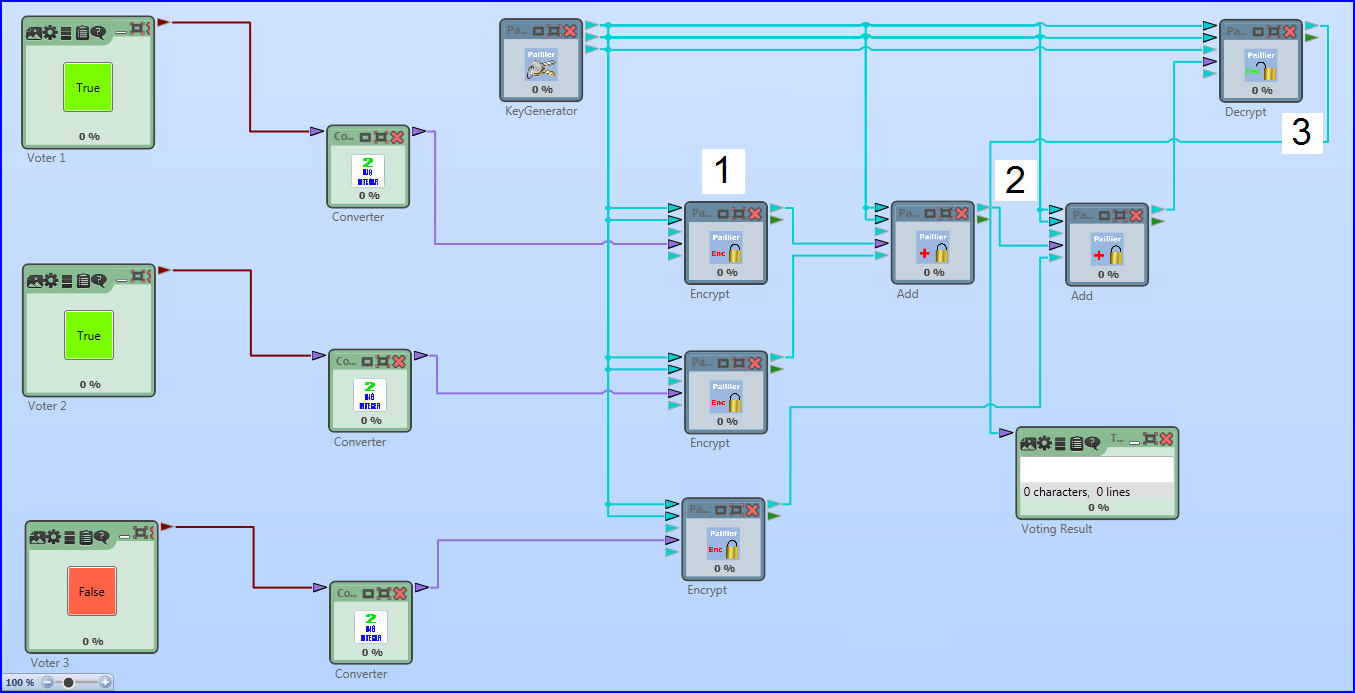
\includegraphics[scale=0.4]{figures/CT2-PaillierVoting.png}
\caption{Voting-Beispiel für Paillier}
\label{CT2-PaillierVoting}
\end{center}
\end{figure}

\item Ein weiteres Anwendungsgebiet für homomorphe Chiffren ist \glqq Secure Multiparty Computation\grqq. Hierbei berechnen mehrere Parteien gemeinsam eine vorgegebene Funktion. Jede der Parteien steuert einen Input für die zu berechnende Funktion bei. Das Ziel der Berechnung ist es, alle Inputs und auch die Zwischenergebnisse geheim zu halten, während nur das Ergebnis der Funktion bekannt wird. Die Verwendung homomorpher Chiffren hilft dabei, diese Berechnungen auf verschlüsselten Daten durchzuführen. Da sich allerdings unter der homomorphen Chiffre von Paillier nur Additionen (und z.B. keine Multiplikationen durchführen lassen), müssen noch weitere geeignete Methoden verwendet werden. Einen guten Einstieg in dieses Thema bietet Wikipedia \cite{Wiki_SMC}.

\item Weiterhin wird erwartet, dass homomorphe Chiffren im Bereich Cloud Computing enorme Vorteile bringen können. Mittels sogenannter voll-homomorpher Kryptosysteme \cite{Wiki_HomEnc} wird es möglich sein, komplette Anwendungen auf verschlüsselten Daten durchzuführen. Hierzu ist es notwendig, dass unter der homomorphen Verschlüsselung die beiden Operationen Addition und Multiplikation durchgeführt werden können (im Gegensatz zum Paillier-Kryptosystem, welches nur die Addition unterstützt). Ein solches Kryptosystem wurde erstmals 2009 von Craig Gentry vorgestellt \cite{Gentry2009}.
\end{enumerate}

% -----------------------------------------------------------------------------
\section{Homomorphe Chiffren in CrypTool}

\subsection{CrypTool~2}
In CrypTool~2\index{CT2} findet man bereits eine Implementierung des Paillier-Kryptosystems (siehe Bild \ref{CT2-Paillier}). Unter den fertigen Vorlagen finden sich Methoden zur Erzeugung der kryptographischen Schlüssel (Paillier Key Generator), ein Beispiel für eine Ver- und Entschlüsselung mittels Paillier (Paillier Text), sowie Beispiele, die die homomorphen Eigenschaften von Paillier aufzeigen (Paillier Addition, Paillier Blinding und Paillier Voting).

\begin{figure}[ht]
\begin{center}
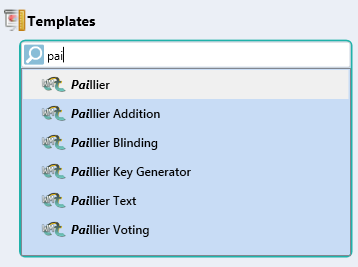
\includegraphics[scale=0.8]{figures/CT2-Paillier.png}
\caption{Paillier-Kryptosystem in CrypTool~2 (CT2)}
\label{CT2-Paillier}
\end{center}
\end{figure}

\newpage

\subsection{JCrypTool}

Im JCrypTool\index{JCT} gibt es eine Implementierung (siehe Bild \ref{JCT-HomEnc}), die die homomorphen Eigenschaften verschiedener Kryptosysteme visualisiert. Für RSA und Paillier wird gezeigt, dass jeweils Multiplikationen (für RSA) und Additionen (für Paillier) auf verschlüsselten Werten möglich sind. Für das voll-homomorphe Kryptosystem von Gentry können sowohl Multiplikationen als auch Additionen auf verschlüsselten Werten durchgeführt werden.

\begin{figure}[ht]
\begin{center}
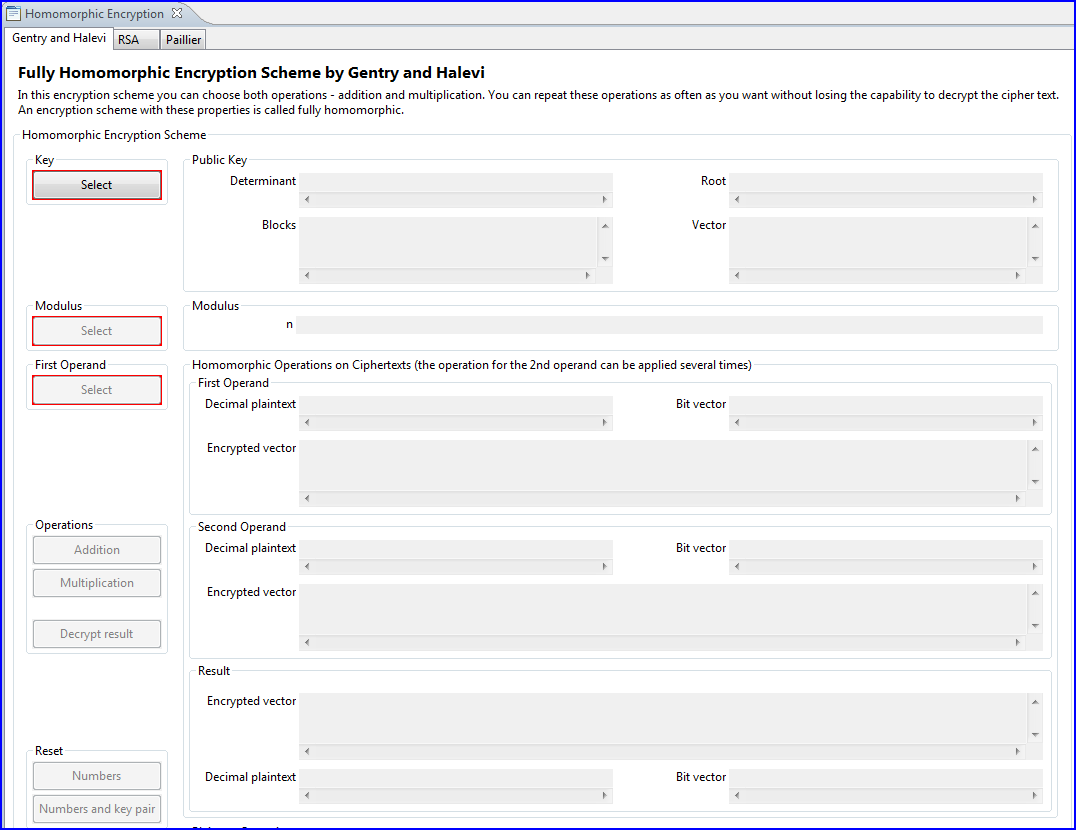
\includegraphics[scale=0.4]{figures/JCT-HomEnc.PNG}
\caption{Kryptosysteme mit homomorphen Eigenschaften in JCrypTool (JCT)}
\label{JCT-HomEnc}
\end{center}
\end{figure}



%------------------------------------------------------------------------------
\printbibliography[%
	heading=subbibintoc,
	title={Literatur zu Kapitel \thechapter},
	segment=\therefsegment,
]


\noindent Alle Links im Artikel wurden am 15.07.2016 überprüft.


\end{refsegment}

% Local Variables:
% TeX-master: "../script-de.tex"
% End:

\renewcommand{\CTBChapName}{(Chap DLogFact)}      % $Id:
% !Mode:: "TeX:DE"    % Setting document mode and submode for WinEdt
% ..............................................................................
% Studie aktuelle akademische Resultate für das Lösen diskreter Logarithmen und zur Faktorisierung
% ~~~~~~~~~~~~~~~~~~~~~~~~~~~~~~~~~~~~~~~~~~~~~~~~~~~~~~~~~~~~~~~~~~~~~~~~~~~~~~
% be_2016-07-14: Housekeeping: " \\\" --> "\\" done (d+E).

\begin{refsegment}




\newcommand{\mmod}{\hspace{1mm}{\rm mod}\hspace{1mm}}
\newcommand{\lf}{\left\lfloor}
\newcommand{\rf}{\right\rfloor}
\newcommand{\norm}{|\!|}


\newcommand{\phin}{\phi(N)}
\newcommand{\bigO}{{\cal O}}
\newcommand{\res}{\textrm{res}}
\newcommand{\poly}{\textrm{poly}}
\newcommand{\dlog}{\textrm{dlog}}
%16xxxxxxxxxxxxxx\newcommand{\bi}{\begin{itemize}}
%16xxxxxxxxxxxxxx\newcommand{\ei}{\end{itemize}}
\newbox\BeweisSym
\setbox\BeweisSym=\hbox{%
\unitlength=0.18ex%
\begin{picture}(10,10)
\put(0,0){\framebox(9,9){}}
\put(0,3){\framebox(6,6){}}
\end{picture}}


\newtheorem{defi}{Definition}
\newtheorem{theo}[defi]{Theorem}
\newtheorem{coro}[defi]{Corollary}
\newtheorem{assu}[defi]{Assumption}
\newtheorem{lemm}[defi]{Lemma}
\newtheorem{prop}[defi]{Proposition}
\newtheorem{nota}[defi]{Notation}
\newtheorem{rema}[defi]{Remark}
\newtheorem{fact}[defi]{Fact}


%--------------------------------------------------------------------
\hypertarget{Chapter_Dlog-FactoringDead}{}
\chapter%[Resultate zur Widerstandskraft diskreter Logarithmen und zur Faktorisierung]
{Studie über aktuelle Resultate für das Lösen diskreter Logarithmen und zur Faktorisierung -- und wie man in der Praxis reagiert}
\chaptermark{Widerstandskraft diskreter Logarithmen}
%
%% \chapter[\texorpdfstring{Studie über aktuelle akademische Resultate für das Lösen diskreter\\ Logarithmen und zur Faktorisierung}{Studie über aktuelle akademische Resultate für das Lösen diskreter Logarithmen und zur Faktorisierung}]{Studie über aktuelle akademische Resultate für das Lösen diskreter Logarithmen und zur Faktorisierung -- und wie man in der Praxis reagiert}% So alles wie gewollt, und auch keine hyperref-Warnung wegen des\\.
                 % \texorpdfstring{X}{Y}  X bekommt man per nameref und steht im normalen Inhaltsverzeichnis;
                 %                        Y steht im Inhaltsverzeichnis links beim Scrollen.
%
%   Ziel war, den längeren Text nur in die Kapitelüberschrift, nicht ins Inhaltsverzeichnis zu bringen, UND
%           nur im Inhaltsverzeichnis-String einen Zeilenumbruch zu erzwingen.
%   \chapter[Studie über aktuelle akademische Resultate für das Lösen diskreter\\ Logarithmen und zur Faktorisierung]{Studie über aktuelle akademische Resultate für das Lösen diskreter Logarithmen und zur Faktorisierung -- und wie man in der Praxis reagiert}% So alles wie gewollt, aber hyperref-Warnung wegen des\\.
% * \chapter[ALTERNATIV für Inhaltsverzeichnis]{ÜBERSCHRIFT}
% * \chapter*{ÜBERSCHRIFT}  (so kein Eintrag ins Inhaltsverzeichnis)
% * \chapter[<short title>]{<title>}
% * https://de.sharelatex.com/learn/Sections_and_chapters
% * \texorpdfstring{<tex>}{<PDF>}
% * \texorpdfstring{Code im Text}{Code für bookmark}
% * Bsp.: \section{  \texorpdfstring{CO\textsubscript{2}} {CO\string_(2)}  }
% * Siehe: http://de.comp.text.tex.narkive.com/3cPmE95e/benutzung-von-texorpdfstring
% * ABER: Nun bei Verwendung von \nameref immer der Umbruch drin und ich schaffte nicht, den wieder rauszubringen.
% * (siehe introduction.tex, Ende von Vorwort, S. xvi)
\label{Chapter_Dlog-FactoringDead}
\index{Logarithmusproblem!diskret}\index{Faktorisierung}

(\hyperlink{author_Antoine-Joux}{Antoine Joux}, \hyperlink{author_Arjen-Lenstra}{Arjen Lenstra} \& \hyperlink{author_Alexander-May}{Alexander May}; April 2014)\\

(Übersetzung ins Deutsche: Patricia Wienen, 2016)\\
% Übersetzung:
% - 'smooth co-factor'  glatter Cofaktor
% - 'Hensel lifting process'   Hensel Lifting bzw. Hensel Lift Prozess
% - 'multiple dlogs'   viele dlogs
% - 'description length'   Beschreibungslänge
% - 'for discrete log-based ?'     'für Dlog-basierte Verfahren ?'



\textbf{Abstract:}
Neuste algorithmische Entwicklungen für das Lösen diskreter Logarithmen in endlichen
Körpern mit kleiner Charakteristik führten zu einer gewissen (publizistisch beförderten)
Unsicherheit bei kryptographischen Nutzern bezüglich des Einflusses auf die Sicherheit kürzlich entwickelter Kryptoverfahren (siehe dazu beispielsweise die Diskussion in~\cite{Blackhat2013} unter dem Stichwort~\glqq Cryptocalypse\grqq).\index{Cryptocalypse}   Dieses Kapitel gibt einen Überblick über die zur Zeit besten Algorithmen für das Berechnen diskreter Logarithmen in verschiedenen Gruppen und über den Status des Faktorisierungsproblems. Unser Ziel ist zu klären, was im Moment algorithmisch machbar ist und wofür erst weitere bedeutende Durchbrüche nötig sind. Zusammenfassend sehen wir im Moment keinen Weg, wie man die bestehenden algorithmischen Prozesse für endliche Körper mit kleiner Charakteristik entweder auf Körper mit großer Charakteristik oder auf das ganzzahlige Faktorisierungsproblem erweitern könnte.
% Our analysis leads to practical mid- and long-term suggestions both for the deployed cryptographic systems and for the choice of their key sizes.


%%%%%
\section{Generische Algorithmen für das Dlog-Problem in beliebigen Gruppen}
\label{generic}

\textbf{Management Summary: Die Widerstandsfähigkeit des diskreten Logarithmus-Pro\-b\-lems
hängt von der Gruppe ab, über die es definiert ist. In diesem Kapitel betrachten wir kryptoanalytische Algorithmen, die für beliebige Gruppen funktionieren. Aus kryptographischem Blickwinkel ist es erstrebenswert, solche Gruppen zu identifizieren, für die sich keine besseren Algorithmen finden lassen. Ein Kandidat dafür sind Gruppen über Elliptischen Kurven.\\[0.1cm]}

In diesem Kapitel beschreiben wir {\em allgemeine} kryptoanalytische Algorithmen, die sich auf {\em jede} endliche abelsche Gruppe anwenden lassen. Das heißt, jede in der Kryptographie verwendete Gruppe -- z. B. multiplikative Gruppen über endlichen Körpern oder über Elliptischen Kurven -- ist für diese Algorithmen anfällig. Wir werden sehen, dass wir mit der Pollard-Rho-Methode in einer Gruppe der Ordnung $n$ immer einen diskreten Logarithmus in $\bigO(\sqrt n)$ Schritten berechnen können. Umgekehrt bedeutet das, dass man eine Gruppe mit einer Ordnung von mindestens $2^{2k}$ wählen muss, um ein Sicherheitslevel von $2^{k}$ zu erreichen. Z.B. muss man für ein Sicherheitslevel von $80$ Bits eine Gruppe der Ordnung $160$ Bits oder mehr wählen. Das erklärt, warum wir in der Praxis üblicherweise Gruppen über Elliptischen Kurven mit einer Ordnung von mindestens $160$ Bits wählen.

Des Weiteren sei $G$ eine Gruppe der Ordnung $n$ und sei $n=p_1^{e_1} \cdot \ldots \cdot p_{\ell}^{e_{\ell}}$ die Primfaktorzerlegung von $n$. Wir werden sehen, dass diskrete Logarithmen in $G$ in Zeit $\bigO(e_1 \sqrt{p_1} + \ldots + e_{\ell}\sqrt{p_{\ell}})$ berechnet werden können. Man bemerke, dass diese Beschränkung äquivalent ist zu Pollard's Beschränkung $O(\sqrt n)$ g.d.w. $n$ prim ist. Andernfalls wird die Komplexität der Berechnung des diskreten Logarithmus hauptsächlich beschränkt durch die Größe des größten Primteilers der Gruppenordnung. Dies erklärt, warum z.B. Schnorr-/DSA-Signaturen in Gruppen implementiert werden, die per Konstruktion einen Primfaktor von mindestens $160$ Bit Länge enthalten. Das erklärt außerdem, warum Gruppen über Elliptischen Kurven üblicherweise primer Ordnung sind oder deren Ordnung nur einen sehr kleinen \textbf{glatten Cofaktor} enthält.


\subsection{Die Pollard-Rho-Methode}
\index{Pollard-Rho}
Sei $G$ eine endliche abelsche Gruppe. Sei $g$ ein Generator einer großen Untergruppe $G' = \{g, g^2, \ldots, g^n\} \subseteq G$ (z.B. könnte $g$ die Gruppe $G$ selbst generieren). Sei $y=g^{x}$. Dann beschreibt das diskrete Logarithmus-Problem den Versuch, bei Eingabe von $g$ und $y$ den Wert $x \mod n$ auszugeben.
Wir schreiben $x=\dlog_g(y)$.

Die Pollard-Rho-Methode versucht, Elemente $g^{a_i}y^{b_i} \in G'$ mit $a_i, b_i \in \mathbb{N}$ in einer pseudozufälligen, aber deterministischen Art und Weise zu erzeugen. Der Einfachheit halber nehmen wir an, dass wir zufällige Elemente von den $n$ Elementen in $G'$ erzeugen. Dann erwarten wir wegen des Geburtstagsparadoxons nach höchstens $\bigO(\sqrt n)$ Schritten zwei identische Elemente zu erhalten. In unserem Fall bedeutet das
$$
  g^{a_i}y^{b_i} = g^{a_j}y^{b_j}.
$$
Dies kann umgeschrieben werden als $g^{\frac{a_i-a_j}{b_j-b_i}} = y$. Daraus wiederum folgt, dass wir unseren diskreten Logarithmus aus $x \equiv \frac{a_i-a_j}{b_j-b_i} \mmod n$ erhalten können.

Somit kann man mit der Pollard-Rho-Methode den diskreten Logarithmus in jeder endlichen abelschen Gruppe der Ordnung $n$ in $\bigO(\sqrt n)$ Schritten berechnen. Durch die Nutzung von Techniken zum Auffinden von Schleifen (sogenannter cycle-finding techniques) kann man außerdem zeigen, dass die Pollard-Rho-Methode mit konstantem Speicherbedarf implementiert werden kann.

Außerdem ist es auch möglich, die Effizienz von Quadratwurzel-Algorithmen zu verbessern, wenn mehrere diskrete Logarithmen in derselben Gruppe erwünscht sind: Bei der Berechnung von $L$ verschiedenen Logarithmen kann man die globalen Kosten von $\bigO (L\sqrt{n})$ auf $\bigO (\sqrt{Ln})$ reduzieren~\cite{multiple2014}.


\subsection{Der Silver-Pohlig-Hellman-Algorithmus}
\index{Silver-Pohlig-Hellman}
Wie zuvor sei $y = g^{x}$ für einen Generator $g$ der Ordnung $n$. Wir wollen den diskreten Logarithmus $x \mmod n$ berechnen. Außerdem sei $n=p_1^{e_1} \cdot \ldots \cdot p_{\ell}^{e_{\ell}}$ die Primfaktorzerlegung von $n$. Dann gilt nach dem Chinesischen Restsatz, dass $x \mmod n$ eindeutig definiert wird durch folgendes System von Kongruenzen:
\begin{equation}
\label{crt}
\begin{array}{lll}
  x & \equiv & x_1 \mmod p_1^{e_1}\\
    & \vdots\\
  x & \equiv & x_{\ell} \mmod p_{\ell}^{e_{\ell}}.	
\end{array}
\end{equation}

Der Algorithmus von Silver-Pohlig-Hellman berechnet alle diskreten Logarithmen $x_i \mmod p_i$ in den Untergruppen mit den Ordnungen $p_i$ in $\bigO(\sqrt{p_i})$ Schritten durch Verwendung der Pollard-Rho-Methode. Danach ist es relativ einfach einen Logarithmus modulo der Primzahlpotenz $x_i \mmod p_i^{e_i}$ mittels eines \textbf{Hensel-Lift-Prozesses} zu finden, der $e_i$ Aufrufe an die diskrete Logarithmus-Prozedur modulo $p_i$ ausführt. In einem \textbf{Hensel-Lift-Prozess} starten wir mit einer Lösung $x_i \mmod p_i$ und berechnen dann nacheinander $x_i \mmod p_i^2$, $x_i \mmod p_i^3$ usw. bis zu $x_i \mmod p_i^{e_i}$ (siehe~\cite{May2013} für Hensels Schema).

Schlussendlich berechnet man den gewünschten diskreten Logarithmus $x \mmod n$ aus dem obigen System von Gleichungen~(\ref{crt}) über den Chinesischen Restsatz.
Insgesamt wird die Laufzeit hauptsächlich festgelegt durch die Berechnung von $x_i \mmod p_i$ für den größten Primfaktor $p_i$. Damit ist die Laufzeit ungefähr $\bigO(\max_i\{\sqrt p_i\})$.


\subsection{Wie man Laufzeiten misst}
Im Verlauf dieser Studie wollen wir die Laufzeit von Analyse-Algorithmen für diskrete Logarithmen abschätzen als Funktion der Bitgröße $n$. Es gilt, dass jede Ganzzahl $n$ mit (ungefähr) $\log n$ Bits geschrieben werden kann, wobei der Logarithmus zur Basis $2$ gewählt wird. Die {\em Bitgröße} von $n$ ist damit $\log n$.

Um unsere Laufzeiten auszudrücken nutzen wir die Notation $L_n[b,c]=\exp^{c \cdot (\ln n)^{b}(\ln\ln n)^{1-b}}$ für Konstanten $b \in [0,1]$ und $c>0$. Bemerke, dass $L_n[1,c]=e^{c \cdot \ln n} = n^c$ eine Funktion ist, die für konstantes $c$ polynomiell in $n$ ist. Deshalb sagen wir, dass $L_n[1,c]$ {\em polynomiell} in $n$ ist. Bemerke außerdem, dass $L_n[1,c]=n^c = (2^{c})^{\log_2 n}$ eine in $\log n$ exponentielle Funktion ist. Deshalb sagen wir, dass $L_n[1,c]$ {\em exponentiell} in der Bitgröße $\log n$ von $n$ ist. Damit erreicht unser Pollard-Rho-Algorithmus eine erwartete Laufzeit von $L[1,\frac 1 2]$.

Auf der anderen Seite ist $L_n[0,c] = e^{c \cdot \ln\ln n} = (\ln n)^c$ {\em polynomiell} in der Bitgröße von $n$. Merke, dass der erste Parameter $b$ für die Laufzeit wichtiger ist als der zweite Parameter $c$, da $b$ zwischen polynomieller und exponentieller Laufzeit interpoliert. Als Kurzschreibweise definieren wir $L_n[b]$, wenn wir die Konstante $c$ nicht spezifizieren wollen.

Einige der wichtigsten Algorithmen, die wir in den nachfolgenden Kapitels besprechen, erreichen eine Laufzeit von $L_n[\frac 1 2 +o(1)]$ oder $L_n[\frac 1 3 +o(1)]$ (wobei das $o(1)$ für $n\to\infty$ verschwindet), welche eine Funktion ist die schneller wächst als jedes Polynom, aber langsamer als exponentiell. Für kryptographische Verfahren sind solche Angriffe völlig akzeptabel, da das gewünschte Sicherheitslevel einfach erreicht werden kann durch moderates Anpassen der Schlüsselgrößen.

Der aktuelle Algorithmus von Joux et al. für die Berechnung diskreter Logarithmen in endlichen Körpern mit kleiner Charakteristik erreicht jedoch eine Laufzeit von $L_n[o(1)]$, wobei $o(1)$ gegen $0$ geht für $n \to \infty$. Das bedeutet, dass diese Algorithmen in quasi-polynomieller Zeit laufen, und dass die zugrunde liegenden Körper nicht länger akzeptabel sind für kryptographische Anwendungen. Ein endlicher Körper $\mathbb{F}_{p^n}$ hat eine kleine Charakteristik, wenn $p$ klein ist, d.h. der Basiskörper (base field) $\mathbb{F}_p$ ist klein und der Grad $n$ der Körpererweiterung ist üblicherweise groß. In den aktuellen Algorithmen brauchen wir ein kleines $p$, da diese Algorithmen über alle $p$ Elemente im Basiskörper $\mathbb{F}_p$ laufen.


\subsection{Unsicherheit durch Quantencomputern}
\index{Quantencomputer}
In 1995 veröffentlichte Shor einen Algorithmus für die Berechnung diskreter Logarithmen und Faktorisierungen auf einem Quantencomputer. Er zeigte, dass die Berechnung diskreter Logarithmen in {\em jeder} Gruppe der Ordnung $n$ in polynomieller Zeit durchgeführt werden kann, die fast $\bigO(\log n^2)$ entspricht. Dieselbe Laufzeit gilt für die Berechnung der Faktorisierung einer Ganzzahl $n$. Diese Laufzeit ist nicht nur polynomiell, die Angriffe sind sogar noch effizienter als die kryptographischen Verfahren selbst! Das wiederum bedeutet, dass das Problem nicht durch bloßes Anpassen der Schlüsselgrößen behoben werden kann.

Sollten wir also in den nächsten Jahrzehnten die Entwicklung groß angelegter Quantencomputer miterleben, muss folglich die ganze klassische, auf Dlog oder Faktorisierung basierende Kryptographie ersetzt werden. Man sollte allerdings betonen, dass die Konstruktion großer Quantencomputer mit vielen Qubits sehr viel schwieriger zu sein scheint als die seines klassischen Gegenstücks, da die meisten kleinen Quantensysteme nicht gut skalieren und ein Problem mit Dekohärenz haben.\\[0.1cm]

\textbf{Empfehlung:} Es scheint schwierig zu sein, die Entwicklungen in der Konstruktion von Quantencomputern vorherzusagen. Experten der Quantenphysik sehen aber derzeit keine unüberwindbaren Hindernisse, die die Entwicklung großer Quantencomputer auf lange Sicht behindern würden. Es dürfte sehr wichtig sein, den aktuellen Fortschritt in diesem Gebiet im Blick zu behalten und in den nächsten 15 Jahren alternative quanten-resistente Kryptoverfahren zur Hand zu haben.\\[0.1cm]

\textbf{Referenzen und weiterführende Literatur:}
Wir empfehlen die Bücher von Menezes, van Oorschot und Vanstone~\cite{Menezes2001}, Joux~\cite{Joux2009} und Galbraith~\cite{Galbraith2012} zur Studie kryptoanalytischer Techniken. Einen einführenden Kurs in Kryptoanalyse stellt Mays Vorlesungsskript zur Kryptoanalyse zur Verfügung~\cite{May2012a,May2012b}. Eine Einleitung zu Quantenalgorithmen findet sich in den Büchern von Homeister~\cite{Homeister2007} und Mermin~\cite{Mermin2008}.

Die Algorithmen in diesem Kapitel wurden ursprünglich in den hervorragenden Arbeiten von Pollard~\cite{Pollard1975,Pollard2000} und Shor~\cite{Shor1994} vorgestellt.
Generische Algorithmen für viele Dlogs wurden kürzlich untersucht in~\cite{multiple2014}.


%%%%%
\section{\texorpdfstring{Beste Algorithmen für Primkörper $\mathbb{F}_p$}{Beste Algorithmen für Primkörper Fp}}
\label{prime_field}
\index{Primkörper}
\textbf{Management Summary: Primkörper $\mathbb{F}_p$ sind -- neben Elliptischen Kurven -- die Standardgruppe für das diskrete Logarithmus-Problem. In den letzten 20 Jahren gab es für diese Gruppen keinen signifikanten algorithmischen Fortschritt. Sie sind immer noch eine gute Wahl für Kryptographie.\\[0.1cm]}

In Kapitel~\ref{generic} haben wir gelernt, dass wir in jeder endlichen abelschen Gruppe der Ordnung $n$ den diskreten Logarithmus in $\bigO(\sqrt n)$ Schritten bestimmen können. Merke, dass sowohl die Pollard-Rho-Methode als auch der Silver-Pohlig-Hellman-Algorithmus aus Kapitel~\ref{generic} keine andere Eigenschaften der {\em Repräsentation} von Gruppenelementen nutzen als ihre Eindeutigkeit. In diesen Methoden werden Gruppenelemente einfach durch Gruppenoperationen und Test auf Gleichheit von Elementen berechnet. Algorithmen dieser Art werden in der Literatur als {\em generisch} bezeichnet.

Es ist bekannt, dass generische Algorithmen diskrete Logarithmen nicht in besserer Zeit als der Silver-Pohlig-Hellman-Algorithmus~\cite{Shoup1997} berechnen können. Damit können die Algorithmen aus Kapitel~\ref{generic} als optimal betrachtet werden, wenn keine weitere Information über die Gruppenelemente bekannt ist.

Wenn wir unsere Gruppe $G$ spezifizieren als die multiplikative Gruppe über den endlichen Körper $\mathbb{F}_p$ mit $p$ prim, können wir sogar die Repräsentation der Gruppenelemente ausnutzen. Natürliche Repräsentanten von $\mathbb{F}_p$ sind die Ganzzahlen $0, \ldots, p-1$. Damit können wir z.B. die Primfaktorzerlegung dieser Ganzzahlen verwenden. Dies wird gemacht in den Algorithmen des sogenannten Typs {\em Index-Calculus} für diskrete Logarithmen. Dieser Typ von Algorithmen bildet derzeit die Klasse mit den besten Laufzeiten für diskrete Logarithmen über Primkörper, prime Körpererweiterungen (Kapitel~\ref{ffs}) und für das Faktorisierungsproblem (Kapitel~\ref{factor}).

Wir werden jetzt einen Index-Calculus-Algorithmus an Hand eines sehr einfachen Beispiels veranschaulichen.


%%%%%
\subsection{Eine Einleitung zu Index-Calculus-Algorithmen}
\label{simple}
\index{Index-Calculus}
Ein Index-Calculus-Algorithmus besteht aus drei grundlegenden Schritten.

\begin{description}
\item[Faktorbasis:] Definition der Faktorbasis $F=\{f_1, \ldots, f_k\}$. Wir wollen die Gruppenelemente ausdrücken als Potenzen von Elementen der Faktorbasis.

\item[Relationen finden:] Finde Elemente $z_i:=g^{x_i} \in G$ für eine ganze Zahl $x_i$, die mit der Faktorbasis bestimmt werden können. Das bedeutet
$$
  g^{x_i} = \prod_{j=1}^k f_j^{e_{ij}}.
$$
Schreiben wir diese Gleichung zur Basis $g$ erhalten wir eine {\em Relation}
$$
  x_i \equiv \sum_{j=1}^k e_{ij}\textrm{dlog}_g(f_j) \mmod n,
$$
wobei $n$ die Ordnung von $g$ ist. Dies ist eine lineare Gleichung in den $k$ Unbekannten $\textrm{dlog}_g(f_1), \ldots, \textrm{dlog}_g(f_k)$. Sobald wir $k$ linear unabhängige Relationen dieses Typs haben, können wir die Unbekannten mit Linearer Algebra berechnen. Das bedeutet, dass wir erst alle diskreten Logarithmen der Faktorbasis berechnen müssen, bevor wir den gewünschten individuellen Logarithmus von $y$ bestimmen.

\item[Dlog-Berechnung:] Drücke $yg^r = g^{x+r} = \prod_{j=1}^k f_j^{e_j}$ in der Faktorbasis für eine ganze Zahl~$r$ aus.
Das gibt uns eine neue Relation
$$
  x+r \equiv \sum_{j=1}^k e_{j}\textrm{dlog}_g(f_j) \mmod n,
$$
die in der einzigen Unbekannten $x=\textrm{dlog}_g y$ einfach gelöst werden kann.
\end{description}

Lassen Sie uns ein einfaches Beispiel für einen Index-Calculus-Algorithmus geben, das $x=\textrm{dlog}_2(5)$ in $\mathbb{F}_{11}^*$ berechnet. Da $2$ die multiplikative Gruppe $\mathbb{F}_{11}^*$ generiert, ist $2$ von der Ordnung $10$.

\begin{description}
\item[Faktorbasis:] Definiere $F=\{-1,2\}$.

\item[Relationen finden:] $2^1 = (-1)^0 2^1$ gibt uns eine erste triviale Relation
$$
  1 \equiv 0 \cdot \textrm{dlog}_2(-1) + 1\cdot \dlog_2(2) \mmod 10.
$$
Wenn wir $2^6 = 64 \equiv -2 \mmod 11$ berechnen, erhalten wir eine zweite Relation
$$
  6 \equiv 1\cdot \dlog_2(-1) + 1 \cdot \dlog_2(2) \mmod 10.
$$
Damit können wir das System von linearen Gleichungen lösen:
$$
\left(
\begin{array}{ll}
0 & 1\\
1 & 1
\end{array}
\right)
\cdot
\left(
\begin{array}{l}
\dlog_2(-1)\\
\dlog_2(2)
\end{array}
\right)
%
\equiv
%
\left(
\begin{array}{l}
1\\
6
\end{array}
\right) \mmod 10.
$$
Als eindeutige Lösung erhalten wir $\dlog_2(-1) \equiv 5$ und $\dlog_2(2) \equiv 1$.

\item[Dlog-Berechnung:] Wegen $5 \cdot 2^{1} = 10 \equiv -1 \mmod 11$ erhalten wir
$$
  x + 1 \equiv 1 \cdot \dlog(-1) + 0 \cdot \dlog(2) \mmod 10.
$$
Dies führt zu der Lösung $x \equiv 4 \mmod 10$.
\end{description}

\textbf{Laufzeit:}
Eine große Faktorbasis zu wählen macht es einfacher, Relationen zu finden, da es die Wahrscheinlichkeit erhöht, dass sich eine bestimmte Zahl in der Faktorbasis aufteilt. Auf der anderen Seite müssen wir für eine große Faktorbasis mehr Relationen finden, um die Dlogs aller Faktorbasiselemente zu berechnen. Eine Optimierung dieses Kompromisses führt zu einer Laufzeit von $L_p[\frac 1 2]$ für den "`relation finding"'-Schritt und ebenfalls $L_p[\frac 1 2]$ für die Berechnung des individuellen diskreten Logarithmus in Schritt~3.

Lasst uns kurz die Vor- und Nachteile des obigen, simplen Index-Calculus-Algorithmus aus der Sicht eines Kryptoanalysten diskutieren.

\textbf{Vorteile:}
\begin{itemize}
\item Für $g^{x_i} = \prod_{j=1}^k f_j^{e_{ij}}$ ist es trivial, den diskreten Logarithmus auf der linken Seite zu berechnen.
\end{itemize}

\textbf{Nachteile:}
\begin{itemize}
\item Wir müssen relativ große Zahlen $g^{x_i}$ über die ganzen Zahlen mit einbeziehen. Man kann zeigen, dass dies zwangsläufig zu einer Laufzeit von $L_p[\frac 1 2]$ führt, und dass es keine Hoffnung gibt, unter die Konstante $\frac 1 2$ zu kommen.
\DIFdelbegin %DIFDELCMD <

\DIFdelend \item Wir müssen alle diskreten Logarithmen für die Faktorbasiselemente berechnen. Dies ist allen Index-Calculus-Algorithmen zu eigen.
\end{itemize}

Wir werden den ersten Nachteil eliminieren, indem wir Faktorisierung über Zahlkörpern erlauben.
Der zweite Nachteil wird eliminiert, indem man eine Faktorbasis wählt, bei der man die Dlogs ihrer Elemente sehr effizient berechnen kann.
%Let us illustrate our Index Calculus in a (trivial) commuting diagram.



\subsection[Das Zahlkörpersieb zur Berechnung des Dlog]{Das Zahlkörpersieb zur Berechnung des Dlog\footnotemark}
\footnotetext{%
   Beim Zahlkörpersieb zur Berechnung des Dlog gibt es -- im Gegensatz zum Zahlkörpersieb
   zur Faktorisierung in Abschnitt~\ref{nfs-factor} -- nur \textbf{das} Zahlkörpersieb.
   Die Unterscheidung Special versus General fällt hier weg.}
\label{nfs-dlog}
\index{Zahlkörpersieb}

Ein Zahlkörper $\mathbb{Q}[\alpha]$ ist ein $k$-dimensionaler Vektorraum über $\mathbb{Q}$ und kann erzeugt werden durch Anfügen einer Nullstelle $\alpha$ eines irreduziblen Polynoms $f$ vom Grad $k$ an $\mathbb{Q}$. Das bedeutet, wir können jedes Element von $\mathbb{Q}[\alpha]$ schreiben als $a_0+a_1\alpha + \ldots a_{k-1}\alpha^{k-1}$ mit $a_i \in \mathbb{Q}$. Wenn wir die $a_i$ auf die ganzen Zahlen beschränken, befinden wir uns im Ring $\mathbb{Z}[\alpha]$.

Das Zahlkörpersieb ist ebenfalls ein Index-Calculus-Algorithmus. Verglichen
mit dem vorigen Ansatz hat er den Vorteil, kleinere Zahlen zu verwenden.
Das wird erreicht durch die Wahl einer spezifischen Repräsentation des
Primkörpers $\mathbb{F}_p$, der implizit definiert ist als endlicher Körper, bei
dem zwei Polynome kleinen Grades mit kleinen Koeffizienten eine gemeinsame
Nullstelle besitzen. Es gibt mehrere Methoden, mit denen man solche Polynome
mit einer gemeinsamen Nullstelle modulo $p$ konstruieren kann. Insbesondere
mit Primzahlen einer speziellen Form, {\it d.h.}\/ mit einer dünn besetzten
Präsentation, ist es möglich, Polynome zu konstruieren, die viel besser sind als im allgemeinen Fall.
Eine typische Konstruktion, die gut funktioniert, ist eine Zahl $m$ zu wählen und
$p$ mit Basis $m$ als $\sum_{i=0}^{t}a_im^i$ zu schreiben. Dann haben $f_1(X)=X-m$
und $f_2(X)=\sum_{i=0}^{t}a_im^i$ den Wert $m$ als gemeinsame Nullstelle modulo $p$.

Ausgerüstet mit zwei Polynomen $f_1$ und $f_2$ von dieser Form, mit $m$ als
gemeinsamer Nullstelle modulo $p$, erhalten wir folgendes kommutatives
Diagramm:
\[
\begin{tikzcd}
\& \mathbb{Z}[X]
\arrow{ld}{}
\arrow{rd}{}
\\
\mathbb{Q}[X]/(f_1(X)) \arrow{rd}{X\mapsto m} \& \&\mathbb{Q}[X]/(f_2(X)) \arrow{ld}{X\mapsto m}\\
\&\mathbb{F}_p\&
\end{tikzcd}
\]

Seien $r_1, r_2$ die Nullstellen von $f_1, f_2$. Wir betrachten die Zahlkörper $\mathbb{Q}[r_1] \simeq \mathbb{Q}[X]/(f_1(X))$ und $\mathbb{Q}[r_2] \simeq \mathbb{Q}[X]/(f_2(X))$.

\begin{description}
\item[Faktorbasis:] Besteht aus primen Elementen mit kleiner Norm aus beiden Zahlkörpern.

\item[Relationen finden:] Das grundlegende Prinzip des Zahlkörpersiebs besteht darin,
  Elemente der Form $a+bX$ an beide Seiten des Diagramms zu senden und eine Relation zu schreiben, wenn sich beide Seiten in die Faktorbasis faktorisieren lassen. Technisch ist das ziemlich herausfordernd, weil wir mehrere Werkzeuge einführen müssen, um zu erklären, dass die linken und rechten Seiten nicht notwendigerweise {\it Faktorielle Ringe} (unique factorization domains) sind. Als Konsequenz müssen wir die Elemente in Ideale faktorisieren und uns um die Hindernisse kümmern, die aus den Idealklassengruppen und Einheitsklassen resultieren.
Diese Prozedur gibt uns den diskreten Logarithmus der Faktorbasiselemente.

\item[Dlog-Berechnung:] Drücke den gesuchten Logarithmus als Linearkombination der Faktorbasiselemente aus.
\end{description}

\textbf{Laufzeit:}
Das Zahlkörpersieb ist der derzeit effizienteste bekannte Algorithmus für das diskrete Logarithmus-Problem mit großer Charakteristik. Im allgemeinen Fall -- d.h. p hat keine spezielle Form, z.B. nah an einer Primzahlpotenz -- ist seine Komplexität $L_p[\frac 1
3,\left(\frac{64}{9}\right)^{1/3}]$.

\textbf{Referenzen und weiterführende Literatur:}
Für eine Einleitung zu Index-Calculus und die damit verbundenen mathematischen Werkzeuge siehe Mays Vorlesungsskript zur Zahlentheorie~\cite{May2013} und das Buch zur Zahlentheorie von M\"uller-Stach, Piontkowski~\cite{MSP2011}. Um ein tieferes Verständnis des Zahlkörpersiebs zu erlangen, sollte man das Buch von Lenstra und Lenstra~\cite{NFS1993} studieren, das alle Originalarbeiten enthält, die zur Entwicklung des Zahlkörpersieb-Algorithmus in den späten 80ern und frühen 90ern geführt haben.

Als guten Start, um das Zahlkörpersieb zu verstehen, empfehlen wir, zunächst seine Vorgänger zu studieren, die in den Originalarbeiten von Adleman~\cite{Adleman1979}, Coppersmith~\cite{CoppersmithOS1986} und Pomerance~\cite{Pomerance1984,Pomerance1996} beschrieben sind.


%%%%%
\section{\texorpdfstring{Beste bekannte Algorithmen für Erweiterungskörper $\mathbb{F}_{p^n}$ und aktuelle Fortschritte}
                        {Beste bekannte Algorithmen für Erweiterungskörper Fpn und aktuelle Fortschritte}}
\label{ffs}
\index{Erweiterungskörper}
\textbf{Management Summary: Die Gruppen über Erweiterungskörpern werden von neuen Algorithmen von Joux et al. angegriffen. Vor der Erfindung dieser Angriffe schien die Sicherheit von Körpererweiterungsgruppen ähnlich der Sicherheit der Gruppen primer Ordnung aus dem letzten Kapitel zu sein. Die neuen Angriffe ließen diese Gruppen völlig unsicher werden, beeinflussten allerdings nicht die Sicherheit der Gruppen primer Ordnung.\\[0.1cm]}

Als erstes werden wir den ehemals besten Algorithmus von 2006 von Joux und Lercier besprechen, der eine Laufzeit von $L_n[\frac 1 3]$ erreicht. Anschließend beschreiben wir aktuelle Entwicklungen, die zu einer dramatischen Verbesserung der Laufzeit zu $L_n[o(1)]$ geführt haben, was quasi polynomiell ist.


\subsection{Der Joux-Lercier Function-Field-Sieve (FFS)}
\index{Function-Field-Sieve (FFS)}
Jeder endliche Körper $\mathbb{F}_{p^n}$ kann repräsentiert werden durch einen Polynomring $\mathbb{F}_p[x]/f(x)$, wobei $f(x)$ ein irreduzibles Polynom über $\mathbb{F}_p$ vom Grad $n$ ist. Damit kann jedes Element in $\mathbb{F}_{p^n}$ durch ein univariates Polynom mit Koeffizienten in $\mathbb{F}_p$ und einem Grad kleiner als $n$ repräsentiert werden. Addition zweier Elemente ist die übliche Addition von Polynomen, wobei die Koeffizienten modulo $p$ genommen werden. Die Multiplikation zweier Elemente ist die übliche Multiplikation von Polynomen, wobei das Ergebnis modulo $f(x)$ reduziert wird, um erneut ein Polynom mit einem Grad kleiner als $n$ zu erhalten.

Es ist wichtig zu bemerken, dass die \textbf{Beschreibungslänge} eines Elementes $n \bigO(\log p)$ ist. Damit erreicht ein polynomieller Algorithmus eine Laufzeit, die polynomiell in $n$ und $\log p$ ist. Wir werden außerdem Körper mit kleiner Charakteristik $p$ in Betracht ziehen, wobei $p$ konstant ist. Dann bedeutet polynomielle Laufzeit polynomiell in $n$.

Es ist bekannt, dass es für jedes $p$ immer Polynome $f(x)$ mit Grad $n$ gibt, die irreduzibel über $\mathbb{F}_p$ sind. Üblicherweise gibt es viele solcher Polynome, was umgekehrt bedeutet, dass wir für verschiedene Polynome $f(x)$ verschiedene Repräsentationen eines endlichen Körpers erhalten. Es ist jedoch ebenfalls bekannt, dass all diese Repräsentationen isomorph sind, und dass Isomorphismen effizient berechenbar sind.

Diese Tatsache wird im Algorithmus von Joux und Lercier verwendet, die verschiedene Repräsentationen $\mathbb{F}_p[x]/f(x)$ und $\mathbb{F}_p[y]/g(y)$ desselben Körpers ausnutzen. Dies wird veranschaulicht durch das folgende kommutative Diagramm.

\[
\begin{tikzcd}
\& \mathbb{F}_{p}[X,Y]
\arrow{ld}{Y \mapsto f(X)}
\arrow{rd}{X \mapsto g(Y)}
\\
\mathbb{F}_{p}[X] \arrow{rd}{X\mapsto x} \& \&\mathbb{F}_p[Y] \arrow{ld}{Y\mapsto y}\\
\&\mathbb{F}_{p^n}\&
\end{tikzcd}
\]

\begin{description}
\item[Faktorbasis:] Wir wählen alle Grad-1 Polynome $x-a$ und $y-b$ aus $\mathbb{F}_p[x] \cup \mathbb{F}_p[y]$. Damit besitzt die Faktorbasis $2p$ Elemente.

\item[Relationen finden:] Auf beiden Seiten, also für Polynome $h$ aus $\mathbb{F}_p[x]/f(x)$ und aus $\mathbb{F}_p[y]/g(y)$, versuchen wir in Linearfaktoren aus der Faktorbasis zu faktorisieren. Das kann für jedes Polynom durch eine einfache ggT-Berechnung $\gcd(h, x^p-x)$ in Zeit $\bigO(p)$ gemacht werden. Man kann zeigen, dass die Anzahl der Polynome, die getestet werden müssen, begrenzt ist durch $L_{p^n}[\frac 1 3]$.
\item[Dlog-Berechnung:] Dieser Schritt wird durchgeführt, indem ein Polynom als Linearkombination von Polynomen kleineren Grades geschrieben und dies rekursiv wiederholt wird, bis Grad-1 gefunden ist. Diese Rekursion wird (Grad-)Abstieg (degree decent) genannt und erfordert ebenso wie der "`relation finding"'-Schritt eine Laufzeit von $L_{p^n}[\frac 1 3]$.
\end{description}


\subsection{Kürzliche Verbesserungen für den Function Field Sieve}
\label{GGMZ}
\index{Function-Field-Sieve (FFS)}

Die erste kürzliche Verbesserung für den Joux-Lercier-FFS wurde präsentiert bei der Eurocrypt~2013 von Joux, der zeigte, dass es möglich ist, die Komplexität für das Finden der Relationen drastisch zu reduzieren, indem man den klassischen siebenden Ansatz durch eine neue Technik ersetzt, die auf der linearen Änderung von Variablen basiert und {\it pinpointing} genannt wird.

\DIFaddend Auf der Crypto Conference 2013 präsentierten G\"ologlu, Granger, McGuire und Zumbr\"agel einen weiteren Ansatz, der mit dem pinpointing verwandt ist und sehr effizient mit Unterkörpern mit Charakteristik 2 arbeitet. Ihr Paper wurde von der kryptographischen Community als so wichtig eingestuft, dass sie den Preis für das beste Paper erhielten.

Die neuen Ergebnisse gelten für endliche Körper $\mathbb{F}_{q^n}$ mit Charakteristik zwei, d.h. $q=2^{\ell}$. Bemerke, dass wir die Standardkonvention\index{Konvention} verwenden, die Primzahlen mit $p$ und Primzahlpotenzen mit $q=p^{\ell}$ bezeichnet.
Für diese Körper $\mathbb{F}_{q^n}$ wird der "`relation finding"'-Schritt im Joux-Lercier-Algorithmus einfacher, da man Polynome konstruieren kann, die sich mit einer höheren Wahrscheinlichkeit teilen lassen als allgemeine Polynome desselben Grades.

Lassen Sie uns eine high-level Beschreibung der Ideen zu ihrer Verbesserungen geben.

\begin{description}
\item[Faktorbasis:] Alle Grad-1 Polynome wie im Joux-Lercier-Algorithmus.

\item[Relationen finden:] G\"ologlu, Granger, McGuire und Zumbr\"agel zeigen, dass man einen speziellen Typ von Polynomen über $\mathbb{F}_q[x]$ konstruieren kann -- die sogenannten Bluher-Polynome -- die sich per Konstruktion über $\mathbb{F}_q[x]$ teilen lassen. Somit erhalten wir ähnlich zu unserer simplen Version des Index-Calculus für ganze Zahlen in Abschnitt~\ref{simple} kostenlos eine Seite der Gleichung. Die Kosten für das Teilen der Polynome in $\mathbb{F}_q[y]$ sind ungefähr $\bigO(q)$, und die Kosten für das Finden des diskreten Logarithmus der Faktorbasiselemente sind ungefähr $\bigO(n \cdot q^2)$. Wir werden weiter unten erklären, warum uns das -- für geeignet gewählte Parameter -- die diskreten Logarithmen der Faktorbasis in {\em polynomieller Zeit} verschafft.

\item[Dlog-Berechnung:] Die Berechnung des individuellen diskreten Logarithmus ist ähnlich wie im Joux-Lercier-Algorithmus.
\end{description}

\textbf{Laufzeit:} Wir rechnen in einem Körper $\mathbb{F}_{q^n}$, mit $q=2^{\ell}$. Somit würde ein Polynomialzeit-Algorithmus eine Laufzeit erfordern, die polynomiell in den Parametern $n$ und $\log q$ ist. Das "`relation finding"' oben benötigt jedoch eine Zeit von $\bigO(n \cdot q^2)$, was polynomiell in $n$ ist, aber exponentiell in $\log q$. Damit arbeitet der Algorithmus aber nur unzureichend, wenn man den Basiskörper $\mathbb{F}_q = \mathbb{F}_{2^{\ell}}$ in Betracht zieht.

Der Trick, um das zu umgehen, ist die Größe der Basis $q$ auf $q'$ zu reduzieren, während man den Erweiterungsgrad $n$ etwas auf $n'$ erhöht. Unser Ziel dabei ist, dass die neue Basiskörpergröße $q'$ ungefähr dem neuen Erweiterungsgrad $n'$ entspricht, also $q' \approx n'$. In diesem Fall erhalten wir erneut eine Laufzeit, die polynomiell in $n'$ und $q'$ ist, aber jetzt ist $q'$ ebenfalls polynomiell beschränkt durch $n'$. Insgesamt ist unsere Laufzeit für Schritt 2 damit polynomiell beschränkt durch $n'$.\\[0.1cm]

Lassen Sie uns ein einfaches Beispiel angeben, wie das für konkrete Parameter gehandhabt wird. Angenommen wir wollen einen diskreten Logarithmus in $\mathbb{F}_{(2^{100})^{100}}$ berechnen. Dann würden wir den Basiskörper zu $q'=2^{10}$ verringern und gleichzeitig den Erweiterungsgrad zu $n'=1000$ erhöhen, d.h. wir rechnen in $\mathbb{F}_{(2^{10})^{1000}}$. Bemerke, dass dies immer gemacht werden kann durch Nutzung effizient berechenbarer Isomorphismen zwischen endlichen Körpern gleicher Kardinalität.\\[0.1cm]

{\em Warnung:} Man könnte versucht sein, das Obige mit der Wahl von Exponenten zu umgehen, die sich nicht geeignet teilen lassen, d.h. durch Wahl von $\mathbb{F}_{2^p}$ mit $p$ prim. Man kann jedoch immer den endlichen Körper in einen größeren Körper einbetten -- ebenso wie die entsprechenden diskreten Logarithmen. Deshalb werden endliche Körper mit kleiner Charakteristik als unsicher angesehen, unabhängig von der speziellen Form des Erweiterungsgrades $n$.\\[0.1cm]

Während das "`relation finding"' in Schritt 2 von G\"ologlu, Granger, McGuire und Zumbr\"agel in {\em polynomieller Zeit} erledigt werden kann, ist die Berechnung des individuellen Logarithmus immer noch zeitraubend. Macht man dies auf naive Art und Weise, ist Schritt 3 wegen des erhöhten Erweiterungsgrades $n'$ sogar noch zeitintensiver als in Joux-Lercier. Balanciert man die Laufzeiten von Schritt 2 und Schritt 3 aus, erhält man eine verbesserte Gesamtlaufzeit von $L_{q^n}[\frac 1 3, (\frac 4 9)^{\frac 1 3}]$.
%\DIFaddbegin \DIFadd{With the pinpointing technique of Joux, the resulting complexity also
%remains of the form $L[\frac 1 3]$.
%}\DIFaddend


\subsection{Quasi-polynomielle Dlog-Berechnung von Joux et al}

Im vorigen Abschnitt wurde gezeigt, dass der diskrete Logarithmus von allen Elementen einer Faktorbasis in polynomieller Zeit berechnet werden kann. Es blieb jedoch ein hartes Problem, diese Tatsache für die Berechnung individueller Logarithmen zu verwenden.

Dieses Problem wurde kürzlich gelöst von Joux~\cite{Joux2013} und Barbulesu, Gaudry, Joux und Thom\'e~\cite{BGJT2013}. Im Paper von Joux wurde gezeigt, dass der individuelle Logarithmus-Schritt in $L[\frac 1 4]$ durchgeführt werden kann. Kurz danach wurde dies verbessert zu $L[o(1)]$ durch Barbulescu, Gaudry, Joux und Thom\'e, was eine Funktion ist, die langsamer wächst als $L[\epsilon]$ für jedes $\epsilon > 0$. Damit erreichen sie quasi-polynomielle Zeit.

Lasst uns kurz die Modifikationen dieser beiden Papers für den Function-Field-Sieve-Algo\-rith\-mus beschreiben.\index{Function-Field-Sieve (FFS)}


\begin{description}
\item[Faktorbasis:] Besteht wie zuvor aus den Grad-1 Polynomen.
\item[Relationen finden:] Man startet mit dem trivialen initialen Polynom
$$
  h(x)= x^q-x = \prod_{\alpha \in \mathbb{F}_q} (x-\alpha)
$$
das sich offensichtlich in die Faktorbasis faktorisieren lässt. Jetzt wendet man lineare und rationale Transformationen (Homographien genannt) auf $h(x)$ an, die seine Eigenschaft, sich über der Faktorbasis faktorisieren zu lassen, erhalten. Man kann zeigen, dass es genügend viele Homographien gibt, um ausreichend viele Relationen zu konstruieren. Somit können wir aus einem trivialen Polynom $h(x)$ kostenfrei alle $\bigO(q)$ Relationen erhalten. Das befähigt uns dazu, die diskreten Logarithmen der Faktorbasiselemente in Zeit $\bigO(q)$ zu berechnen.
\item[Dlog-Berechnung:] Barbulescu et al präsentieren einen effizienten {\em Gradabstiegs}-Algorithmus, der bei Eingabe eines Polynoms $p(x)$ von Grad $n$ eine lineare Relation zwischen dem diskreten Logarithmus von $p(x)$ und $\bigO(nq^2)$ Polynomen von Grad $\frac n 2$ ausgibt, in einer Zeit, die polynomiell in $q$ und $D$ ist. Das bedeutet, dass wir einen Baum von Polynomen bekommen, bei dem der Grad mit jedem Level um den Faktor zwei fällt, was umgekehrt eine Baumtiefe von $\log n$ impliziert. Das resultiert in einer Laufzeit von $\bigO(q^{\bigO(\log n)})$.
\end{description}

\textbf{Laufzeit:}
Wie im vorigen Abschnitt~\ref{GGMZ} nehmen wir an, dass die Größe $q$ des Basiskörpers die gleiche Größe hat wie der Erweiterungsgrad $n$, d.h. $q=\bigO(n)$. Dann läuft Schritt 2 in Zeit $\bigO(q)=\bigO(n)$, was polynomiell in $n$ ist. Schritt 3 läuft in Zeit $\bigO(q^{\bigO(\log n)})=\bigO(n^{\bigO(\log n)}) = L_{q^n}[o(1)]$. Bemerke, dass $n^{\log n}=2^{\log^2 n}$ schneller wächst als jede polynomielle Funktion in $n$, aber langsamer als jede sub-exponentielle Funktion $2^{n^{c}}$ für ein $c>0$.


\subsection{Schlussfolgerungen für endliche Körper mit kleiner Charakteristik}

Um einige Beispiele zu geben, was die theoretische quasi-polynomielle Laufzeit der vorigen Ergebnisse in der Praxis bedeutet, veranschaulichen wir in Tabelle~\ref{dlog-table}, was derzeit bei der Berechnung diskreter Logarithmen erreicht werden kann.

\begin{table}[h]
\begin{center}
\begin{tabular}{ccccc}
Datum & Körper & Bitgröße & Kosten (CPU-Stunden) & Algorithmus\\
\hline
 2012/06/17&$3^{6\cdot 97}$ & 923 & 895\,000 & \cite{JL2006}\\
2012/12/24&$p^{47}$ & 1175 & 32\,000 & \cite{Pin2013}\\
2013/01/06&$p^{57}$ & 1425 & 32\,000 & \cite{Pin2013}\\
2013/02/11 &$2^{1778}$ & 1778 & 220 & \cite{Joux2013}\\
2013/02/19 &$2^{1778}$ & 1991 & 2200 & \cite{GGMZ2013}\\
2013/03/22 &$2^{4080}$& 4080 & 14\,100 & \cite{Joux2013}\\
2013/04/11&$2^{6120}$ & 6120 & 750 & \cite{Joux2013}\\
2013/05/21&$2^{6168}$ & 6168 & 550 & \cite{Joux2013}\\
\hline
\end{tabular}
\caption{Rekorde für kleine Charakteristik}
\label{dlog-table}
\end{center}
\end{table}

\textbf{Empfehlung:}
Der Gebrauch von Körpern mit kleiner Charakteristik für Dlog-basierte Verfahren auf Basis diskreter Logarithmen ist \textbf{gänzlich unsicher}, unabhängig davon welche Schlüsselgröße verwendet wird. Glücklicherweise wird davon -- nach unserem Wissen -- in weit verbreiteten/standardisierten kryptographischen Verfahren kein Gebrauch gemacht.



\subsection{Lassen sich diese Ergebnisse auf andere
Index-Calculus-Algo\-rithmen übertragen?}
\index{Index-Calculus}

Aus der Sicht eines Kryptoanwenders würde man sich sorgen, dass sich die aktuellen bahnbrechenden Ergebnisse, die die Komplexität für die Berechnung diskreter Logarithmen in Körpern mit kleiner Charakteristik von $L[\frac 1 3]$ auf $L[o(1)]$ senken, auch auf diskrete Logarithmen in anderen Gruppen anwenden lassen. Man könnte zum Beispiel besorgt sein über das tatsächliche Sicherheitslevel von auf diskreten Logarithmen basierender Kryptographie in endlichen Körpern $\mathbb{F}_p$ mit {\em großer} Charakteristik.\\[0.1cm]

\textbf{Vermutung:} Wir glauben, dass sich die neuen Techniken nicht auf endliche Körper mit großer Charakteristik oder auf Elliptische Kurven übertragen lassen, die gegenwärtig den Standard für kryptographische Konstruktionen darstellen.\\[0.1cm]

Lasst uns kurz einige Gründe sammeln, warum sich die aktuellen Techniken nicht auf diese Gruppen übertragen lassen, und welche Probleme gelöst werden müssen, bevor wir einen signifikanten Fortschritt in der Laufzeit für diese Gruppen sehen.

\begin{itemize}
\item \textbf{Laufzeit:} Man bemerke, dass alle in diesem Abschnitt beschriebenen Index-Calculus-Algorithmen polynomiell in der Größe $q$ des Basiskörpers sind und somit exponentiell in der Bitlänge $\bigO(\log q)$. Damit scheint sich die Härte des diskreten Logarithmus-Problems von der Härte im Basiskörper abzuleiten, wobei der Erweiterungsgrad $n$ nicht dazu beiträgt das Problem erheblich schwieriger zu machen.

Insbesondere merken wir an, dass jede -- wie in den Algorithmen für kleine Charakteristik aus dem Polynom $x^q-x$ konstruierte -- Gleichung mindestens $q$ Terme enthält. Damit würde, sobald $q$ größer als $L[1/3]$ wird, sogar das Schreiben einer einzigen Gleichung dieses Typs mehr kosten als die volle Komplexität des Zahlkörpersiebs aus Abschnitt~\ref{nfs-dlog}.

Bemerke, dass es eine ähnliche Situation für diskrete Logarithmen in Gruppen Elliptischer Kurven gibt. Nutzen wir eine Elliptische Kurve über $\mathbb{F}_q$, ist im Allgemeinen der beste bekannte Algorithmus der generische Pollard-Rho-Algorithmus aus Kapitel~\ref{generic} mit der Laufzeit $\bigO(\sqrt q)$. Allerdings benötigt Gaudry's Algorithmus -- den wir in Abschnitt~\ref{gaudry} besprachen -- für Elliptische Kurven über $\mathbb{F}_{q^n}$ nur eine Laufzeit von $q^{2-\frac 2 n}$, was wesentlich besser ist als die generische Grenze $\bigO(q^{\frac n 2})$. Wie die Algorithmen in diesem Kapitel ist auch Gaudry's Algorithmus ein Index-Calculus-Algorithmus. Und ähnlich wie bei den Algorithmen in diesem Kapitel scheint die Komplexität des diskreten Logarithmus-Problems im Parameter $q$ statt im Parameter $n$ konzentriert zu sein.

\item\textbf{Polynome versus Zahlen:} Bemerke, dass die aktuellen Ergebnisse starken Gebrauch von polynomieller Arithmetik und Unterkörpern von $\mathbb{F}_{q^n}$ machen. Allerdings ist weder die polynomielle Arithmetik verfügbar für $\mathbb{F}_p$ noch existieren Unterkörper für Gruppen primer Ordnung. Wir möchten argumentieren, dass viele Probleme für Polynome effizient lösbar sind, während sie bekanntermaßen hart für ganze Zahlen zu sein scheinen. Es ist zum Beispiel bekannt, dass Polynome über endliche Körper und über rationale Zahlen von den Algorithmen von Berlekamp und Lenstra-Lenstra-Lovasz effizient faktorisiert werden können, während es keinen äquivalenten Algorithmus für ganze Zahlen gibt. Nach von zur Gathen gibt es auch einen effizienten Algorithmus um kürzeste Vektoren in Polynomringen zu finden, während das Gegenstück in Ganzahlgittern (integer lattice) NP-hart ist.

Was ganze Zahlen eigentlich härter macht als Polynome ist der Effekt der Übertragsbits. Multiplizieren wir zwei Polynome, dann wissen wir durch das Konvolutionsprodukt genau, welche Koeffizienten bei welchen Koeffizienten des Produktes mitwirken, was aber bei der Multiplikation ganzer Zahlen wegen der Übertragsbits nicht der Fall ist.

\item\textbf{Komplexität der Schritte 2 \& 3:} Jeglicher algorithmische Durchbruch für diskrete Logarithmen vom Typ Index-Calculus müsste die diskreten Logarithmen einer wohldefinierten Faktorbasis effizient lösen {\em und} den gewünschten Logarithmus in Termen aus dieser Faktorbasis ausdrücken. Zur Zeit haben wir aber im Fall großer Primkörper $\mathbb{F}_p$ für keinen dieser Schritte eine effiziente Methode.
\end{itemize}

\textbf{Referenzen und weiterführende Literatur:}
Coppersmiths Algorithmus~\cite{Coppersmith1984} aus der Mitte der 80er war lange Zeit die Referenzmethode für die Berechnung diskreter Logarithmen in Körpern mit kleiner Charakteristik. Der Joux-Lercier-Function-Field-Sieve wurde 2006 in~\cite{JL2006} vorgestellt.\index{Function-Field-Sieve (FFS)}

Die aktuellen Fortschritte begannen auf der Eurocrypt 2013 mit Jouxs Pinpointing-Tech\-nik~\cite{Pin2013}. Auf der Crypto 2013 verbesserten G\"ologlu, Granger, McGuire und Jens Zumbr\"agel~\cite{GGMZ2013} bereits die Konstante $c$ in der $L[\frac 1 3,c]$-Laufzeit. Die Verbesserung zur Laufzeit $L[\frac 1 4]$ wurde dann vorgestellt in der Arbeit von Joux~\cite{Joux2013}. Letztendlich schlugen Barbulescu, Gaudry, Joux und Thom{\'e}~\cite{BGJT2013} einen Algorithmus für den Abstieg vor, der zur Laufzeit $L[o(1)]$ führte.


%%%%%
\section{Beste bekannte Algorithmen für die Faktorisierung natürlicher Zahlen}
\label{factor}
\index{Faktorisierung}
\textbf{Management Summary: Der beste Algorithmus zur Faktorisierung zeigt starke Ähnlichkeit zum besten Algorithmus für die Berechnung diskreter Logarithmen in Gruppen primer Ordnung. Es scheint, dass die neuen Angriffe nicht dabei helfen, einen der beiden Algorithmen zu verbessern.\\[0.1cm]}

Der beste Algorithmus für die Berechnung der Primfaktorzerlegung einer ganzen Zahl, das sogenannte Zahlkörpersieb, ist dem besten Algorithmus für die Berechnung diskreter Logarithmen in $\mathbb{F}_p$ aus Abschnitt~\ref{nfs-dlog} sehr ähnlich. Sehr viel weniger ähnelt er dem Algorithmus für $\mathbb{F}_{q^n}$ aus Kapitel~\ref{ffs}.

Kurz gesagt beruhen alle bekannten, komplexen Algorithmen, die RSA-Module $n=pq$ für $p,q$ prim faktorisieren, auf derselben simplen, grundlegenden Idee. Unser Ziel ist es, $x, y \in \mathbb{Z}/n\mathbb{Z}$ zu konstruieren so dass
\begin{center}
  $x^2 \equiv y^2 \mmod n$ und $x \not\equiv \pm y \mmod n$.
\end{center}
Dies liefert sofort die Faktorisierung von $n$, da $n$ wegen der ersten Eigenschaft das Produkt $x^2- y^2 = (x+y)(x-y)$ teilt, aber wegen der zweiten Eigenschaft teilt $n$ weder $x+y$ noch $x-y$. Damit teilt ein Primfaktor von $n$ den Term $x+y$, während der andere $x-y$ teilen muss. Das bedeutet umgekehrt, dass $\gcd(x \pm y, n) = \{p,q\}$.

Die Faktorisierungsalgorithmen unterscheiden sich nur in der Art, in der die $x,y$ berechnet werden. Die Absicht ist, $x,y$ mit $x^2 \equiv y^2 \mmod n$ in einer "`unabhängigen"' Art und Weise zu berechnen.
% Remark:
% Ein triviales Beispiel für "dependent" wäre: Wähle $x$ zufällig und setze $y=x$ oder $y=-x$.
% Die Berechnung von y sollte an keiner Stelle das x verwenden.
Falls diese Unabhängigkeit gegeben ist, ist es einfach zu zeigen, dass $x \not\equiv \pm y \mmod n$ mit Wahrscheinlichkeit $\frac 1 2$ gilt, da nach dem Chinesischen Restsatz jedes Quadrat in $\mathbb{Z}/n\mathbb{Z}$ 4 Quadratwurzel besitzt -- zwei verschiedene Wurzeln modulo $p$ und zwei verschiedene Wurzeln modulo $q$.



\subsection[Das Zahlkörpersieb zur Faktorisierung (GNFS)]{Das Zahlkörpersieb zur Faktorisierung (GNFS)\footnotemark}
\footnotetext{%
   Mit Zahlkörpersieb (Number Field Sieve) ist hier immer das \textbf{Allgemeine} Zahlkörpersieb (GNFS) gemeint.
   Im Gegensatz zu Abschnitt~\ref{nfs-dlog} unterscheidet man bei der Faktorisierung zwischen
   einem Special und General Number Field Sieve.\\
   CT2\index{CT2} enthält eine Implementierung des GNFS mittels msieve und YAFU.
}
\label{nfs-factor}
\index{Zahlkörpersieb}

Sei $n \in \mathbb{N}$ die ganze Zahl, die wir faktorisieren wollen. Der Zahlkörpersieb-Algorithmus startet damit, zwei Polynome $f,g$ zu konstruieren, die eine gemeinsame Nullstelle $m$ modulo $N$ teilen. Üblicherweise wird das gemacht, indem man $g(X)=X-m \mmod n$ definiert und ein Polynom $f(X)$ kleinen Grades konstruiert mit $f(m) \equiv 0 \mmod n$ (z.B. durch Erweitern von $n$ zur Basis $m$ wie in Abschnitt~\ref{nfs-dlog}).

Da $f$ und $g$ verschieden sind, definieren sie verschiedene Ringe $\mathbb{Z}[X]/f(X)$ und $\mathbb{Z}[X]/g(X)$. Da aber $f$ und $g$ die gleiche Nullstelle $m$ modulo $n$ teilen, sind beide Ringe isomorph zu $\mathbb{Z}/n\mathbb{Z}$; und dieser Isomorphismus kann explizit berechnet werden durch Mappen von $X \mapsto m$. Dies wird im folgenden kommutativen Diagramm illustriert.
\[
\begin{tikzcd}
\& \mathbb{Z}[X]
\arrow{ld}{}
\arrow{rd}{}
\\
\mathbb{Q}[X]/(f(X)) \arrow{rd}{X\mapsto m} \& \&\mathbb{Q}[X]/(g(X)) \arrow{ld}{X\mapsto m}\\
\&\mathbb{Z}/n\mathbb{Z}\&
\end{tikzcd}
\]

\begin{description}
\item[Faktor base:] Besteht aus primen Elementen mit kleiner Norm aus beiden Zahlkörpern.

\item[Relationen finden:] Wir suchen nach Argumenten $\tilde x$, so dass sich gleichzeitig $\pi_f:=f(\tilde x)$ in $\mathbb{Q}[X]/(f(X))$ und $\pi_g:=g(\tilde x)$ in $\mathbb{Q}[X]/(g(X))$ in die Faktorbasiselemente teilen lassen. Solche Elemente werden Relationen genannt.

\item[Lineare Algebra:] Mit Hilfe Linearer Algebra suchen wir ein Produkt der Elemente $\pi_f$, das ein Quadrat ist und dessen korrespondierendes Produkt der $\pi_g$ ebenfalls ein Quadrat ist. Bilden wir diese Elemente mit unserem Homomorphismus $X \mapsto m$ auf $\mathbb{Z}/n\mathbb{Z}$ ab, so erhalten wir Elemente $x^2,y^2 \in \mathbb{Z}/n\mathbb{Z}$, so dass $x^2 \equiv y^2 \mmod n$. Berechnen wir erst die Quadratwurzeln von $\pi_f$ und $\pi_g$ in deren entsprechenden Zahlkörpern, ohne vorher den Homomorphismus anzuwenden, so erhalten wir wie gewünscht $x, y \in \mathbb{Z}/n\mathbb{Z}$ mit $x^2 \equiv y^2 \mmod N$. Die Unabhängigkeit von $x,y$ leitet sich ab aus den verschiedenen Repräsentationen in beiden Zahlkörpern.
\end{description}

\textbf{Laufzeit:}
Der obige Algorithmus ist bis auf manche Details -- z.B. die Quadratwurzelberechnung im Zahlkörper -- identisch zum Algorithmus aus Abschnitt~\ref{nfs-dlog} und besitzt die gleiche Laufzeit $L[\frac 1
3,\left(\frac{64}{9}\right)^{1/3}]$.


\subsection{\texorpdfstring{Die Verbindung zum Index-Calculus-Algorithmus in $\mathbb{F}_p$}{Die Verbindung zum Index-Calculus-Algorithmus in Fp}}
\index{Index-Calculus}

Erstens wissen wir, dass die Berechnung diskreter Logarithmen in Gruppen $\mathbb{Z}/n\mathbb{Z}$ mit zusammengesetzter Ordnung mindestens so hart ist wie das Faktorisieren von $n=pq$. Das bedeutet umgekehrt, dass jeder Algorithmus, der diskrete Logarithmen in $\mathbb{Z}/n\mathbb{Z}$ berechnet, im Prinzip die Faktorisierung von $n$ berechnet:
\begin{center}
  Dlogs in $\mathbb{Z}/n\mathbb{Z}$ $\Rightarrow$ Faktorisierung von $n$.
\end{center}

Lasst uns kurz die Idee dieser Faktorisierung beschreiben. Wir berechnen die Ordnung $k=\textrm{ord}(a)$ für ein beliebiges $a \in \mathbb{Z}/n\mathbb{Z}$ durch unseren Dlog-Algorithmus, d.h. wir berechnen die kleinste positive Ganzzahl $k$, s.d. $a^{k} \equiv 1 \mmod n$. Ist $k$ gerade, dann ist $a^{\frac k 2} \not\equiv 1$ eine Quadratwurzel von $1$. Wir haben $a^{\frac k 2} \not\equiv -1$ mit einer Wahrscheinlichkeit von mindestens $\frac 1 2$, da die $1$ genau 4 Quadratwurzeln modulo $n$ besitzt. Setze $x \equiv a^{\frac k 2} \mmod n$ und $y = 1$. Dann erhalten wir $x^2 \equiv 1 \equiv y^2 \mmod n$ und $x \not \equiv \pm y \mmod n$. Laut der Diskussion am Beginn des Kapitels erlaubt uns das, $n$ zu faktorisieren.\\[0.1cm]

Zweitens wissen wir außerdem, dass beide Probleme, das Faktorisieren und das Berechnen diskreter Logarithmen in $\mathbb{F}_p$, zusammen mindestens so hart sind wie das Berechnen diskreter Logarithmen in $\mathbb{Z}/n\mathbb{Z}$. Kurz gesagt:
\begin{center}
  Faktorisierung + Dlogs in $\mathbb{F}_p$ $\Rightarrow$ Dlogs in $\mathbb{Z}/n\mathbb{Z}$.
\end{center}
% Remark:
% Wenn man faktorisieren kann UND Dlogs in F_p berechnen kann, dann
% kann man auch Dlogs in Z/nZ berechnen.
% D.h. nicht, dass man beide berechnen können MUSS, der Pfeil geht nur in
% eine Richtung. Der nachfolgende Text erklärt, wie beide Algorithmen
% verwendet werden, um das Problem auf der rechten Seite zu lösen.
Diese Tatsache kann einfach gesehen werden, indem man bemerkt, dass Faktorisierung und Dlogs in $\mathbb{F}_p$ zusammen direkt eine effiziente Version des Silver-Pohlig-Hellman-Algorithmus aus Abschnitt~\ref{generic} geben. Erst faktorisieren wir die Gruppenordnung $n$ in die Primzahlpotenzen $p_i^{e_i}$ und berechnen dann den diskreten Logarithmus in $\mathbb{F}_{p_i}$ für jedes $i$. Genau wie im Silver-Pohlig-Hellman-Algorithmus heben wir die Lösung modulo $p_i^{e_i}$ und kombinieren diese gehobenen Lösungen mittels Chinesischem Restsatz.

Wir möchten betonen, dass diese zwei bekannten Relationen nicht viel darüber aussagen, ob es eine Reduktion
\begin{center}
  Faktorisierung $\Rightarrow$ Dlog in $\mathbb{F}_p$ \hskip 1cm oder \hskip 1cm Dlog in $\mathbb{F}_p \Rightarrow $ Faktorisierung.
\end{center}
gibt.
Beide Richtungen sind ein lang bekanntes offenes Problem in der Kryptographie. Merke jedoch, dass die besten Algorithmen für Faktorisierung und Dlog in $\mathbb{F}_p$ aus den Abschnitten~\ref{nfs-dlog} und~\ref{nfs-factor} bemerkenswert ähnlich sind. Außerdem bedeutete historisch ein Fortschritt bei einem Problem immer auch Fortschritt beim anderen. Obwohl wir keinen formellen Beweis haben, dürfte es fair sein zu sagen, dass beide Probleme aus algorithmischer Sicht eng verknüpft zu sein scheinen.


\subsection{Integer-Faktorisierung in der Praxis}
\index{Faktorisierung}

Gegeben den aktuellen Stand der Technik der akademischen Forschung über Integer-Faktori\-sierung
stellen selbst RSA-Module moderater -- aber sorgfältig gewählter -- Größe einen angemessenen Grad an Sicherheit gegen offene kryptoanalytische Anstrengungen der Community dar. Die größte RSA-Challenge, die durch öffentliche Anstrengungen faktorisiert wurde, hatte lediglich 768 Bits~\cite{factor768_2010} und erforderte ein Äquivalent von etwa 2000 Jahren Berechnung auf einem einzelnen 2 GHz-Kern. Ein Angriff auf 1024-Bit RSA-Module ist etwa tausendmal härter. Ein solcher Aufwand sollte für akademische Anstrengungen für mehrere weitere Jahre außer Reichweite sein. Eine Verdopplung der Größe zu 2048-Bit Modulen erhöht den rechnerischen Aufwand um einen weiteren Faktor von $10^9$. Ohne substantielle neue, mathematische oder algorithmische Erkenntnisse muss 2048-Bit RSA für mindestens zwei weitere Jahrzehnte als außer Reichweite betrachtet werden.


\subsection{\texorpdfstring{Die Relation von Schlüsselgröße versus Sicherheit für Dlog in $\mathbb{F}_p$ und Faktorisierung}{Die Relation von Schlüsselgröße versus Sicherheit für Dlog in Fp und Faktorisierung}}
\label{key-size-factoring}

Die Laufzeit des besten Algorithmus für ein Problem definiert den Sicherheitslevel eines Kryptosystems. Z.B. brauchen wir für 80-Bit Sicherheit, dass der beste Algorithmus
%%% Man könnte hier "im Durchschnitt" ergänzen? ABER:
%%% "in average" suggeriert, dass der Algorithmus probabilistisch ist (was
%%% er nicht sein müsste, aber meistens ist). Kann man machen, wenn man will ...
mindestens $2^{80}$ Schritte benötigt.

Wie wir bereits anmerkten, ist die beste Laufzeit für diskrete Logarithmen in $\mathbb{F}_p$ und für Faktorisierung $L[\frac 1 3,\left(\frac{64}{9}\right)^{1/3}]$. Der akkurateste Weg, diese Formel zu nutzen, ist in der Tat, die Laufzeit für eine große reale Faktorisierung/Dlog-Berechnung zu messen und dann große Werte zu extrapolieren. Angenommen wir wissen, dass es Zeit $T$ brauchte, eine Zahl $n_1$ zu faktorisieren. Dann extrapolieren wir die Laufzeit für ein $n_2 > n_1$ mit der Formel

$$
  T  \cdot \frac{ L_{n_1}[\frac 1
3,\left(\frac{64}{9}\right)^{1/3}] }
{ L_{n_2}[\frac 1
3,\left(\frac{64}{9}\right)^{1/3}] }.
$$

Somit nutzen wir die L-Formel, um den relativen Faktor abzuschätzen, den wir zusätzlich aufwenden müssen. Merke, dass dies die Sicherheit (geringfügig) überschätzt, da die L-Formel asymptotisch ist und somit im Zähler akkurater ist als im Nenner -- der Nenner sollte einen größeren Fehler-Term beinhalten. Somit erhält man in der Praxis eine (nur geringfügig) kleinere Sicherheit als von der Formel vorhergesagt.

Wir berechneten die Formel für mehrere Bitgrößen einer RSA-Zahl $n$, beziehungsweise eine Dlog Primzahl $p$, in Tabelle~\ref{nfs-table}. Man erinnere sich von Abschnitt~\ref{nfs-factor}, dass die Laufzeit des Number-Field-Sieve-Algorithmus für Faktorisierung tatsächlich eine Funktion in $n$ und nicht in den Primfaktoren von $n$ ist.


Wir beginnen mit RSA-768, das 2009 erfolgreich faktorisiert wurde~\cite{factor768_2010}. Um die Anzahl der Instruktionen für die Faktorisierung von RSA-768 zu zählen, muss man definieren, was eine {\em Instruktionseinheit} (instruction unit) ist. In der Kryptographie ist es ein bewährtes Verfahren, die Zeit für die Berechnung von DES als Maßeinheit zu definieren, um eine Vergleichbarkeit von Sicherheitsleveln zwischen Secret- und Public-Key-Primitiven zu erhalten. Dann bietet DES nach Definition dieser Maßeinheit 56-Bit Sicherheit gegen Brute-force-Schlüsselangriffe.

In Bezug auf diese Maßeinheit benötigt die Faktorisierung von RSA-768 $T=2^{67}$ Instruktionen. Von diesem Startpunkt aus extrapolierten wir das Sicherheitslevel für größere Bitgrößen in Tabelle~\ref{nfs-table}.

Wir erhöhten nacheinander die Bitgröße um $128$ bis zu $2048$ Bits. Wir sehen, dass dies zu Beginn zu einem Anstieg der Sicherheit um etwa 5 Bits pro 128-Bit Schritt führt, während wir gegen Ende nur einen Anstieg von etwa 3 Bits pro 128-Bit Schritt haben.

Nach Moores Gesetz verdoppelt sich die Geschwindigkeit von Computern alle 1,5 Jahre. Damit haben wir nach $5\cdot 1,5 = 7,5$ Jahren einen Anstieg von $2^5$, was bedeutet, dass wir derzeit alle $7,5$ Jahre unsere Bitgröße um etwa $128$ Bits erhöhen sollten; und wenn wir uns den $2000$ Bits nähern, sollten die Intervalle unserer Erhöhung in 128-Bit Schritten nicht länger sein als 4,5 Jahre. Für vorsichtigere Wahlen, die außerdem einen gewissen algorithmischen Fortschritt voraussetzt statt nur einen Anstieg in der Geschwindigkeit von Computern, siehe die Empfehlungen in Kapitel~\ref{advice}.

\begin{table}
\begin{center}
\begin{tabular}{c|c}
Bitgröße & Sicherheit\\
\hline
768 & 67.0\\
896 & 72.4\\
1024 & 77.3\\
1152 & 81.8\\
1280 & 86.1\\
1408 & 90.1\\
1536 & 93.9\\
1664 & 97.5\\
1792 & 100.9\\
1920 & 104.2\\
2048 & 107.4\\
\end{tabular}
\caption{Bitgröße von $n$, $p$ versus Sicherheitslevel}
\label{nfs-table}
\end{center}
\end{table}

%%##
%Moreover, the $L$-function can be easily


\textbf{Referenzen und weiterführende Literatur:}
Eine Einleitung zu mehreren Faktorisierungsalgorithmen inklusive des Quadratic Sieve -- dem Vorgänger des Zahlkörpersiebs -- findet sich in Mays Skript zur Zahlentheorie~\cite{May2013}. Wir empfehlen Bl\"omers Skript zur Algorithmischen Zahlentheorie~\cite{Bloemer1999} als Einleitung zum Zahlkörpersieb.

Die Entwicklung des Zahlkörpersiebs wird beschrieben im Lehrbuch von Lenstra und Lenstra~\cite{NFS1993}, das alle Originalarbeiten beinhaltet. Die Relation von diskreten Logarithmen und Faktorisierung wurde diskutiert von Bach~\cite{Bach1984}. Details zum aktuellen Faktorisierungsrekord für RSA-768 kann man in~\cite{factor768_2010} finden.



%%%%%
\section{\texorpdfstring{Beste bekannte Algorithmen für Elliptische Kurven $E$}{Beste bekannte Algorithmen für Elliptische Kurven E}}
\index{elliptische Kurve}

\textbf{Management Summary: Elliptische Kurven sind die zweite Standardgruppe für das diskrete
Logarithmus-Problem. Die neuen Angriffe betreffen diese Gruppen nicht, und ihre Sicherheit bleibt unverändert.\\[0.1cm]}

Wir möchten Elliptische Kurven $E[p^n]$ über endlichen Erweiterungskörpern $\mathbb{F}_{p^n}$ und elliptische Kurven $E[p]$ über Primkörpern $\mathbb{F}_p$ diskutieren. Die letzteren werden üblicherweise für kryptographische Zwecke verwendet. Der Grund, aus dem wir auch die ersteren diskutieren, ist -- ähnlich wie in den vorigen Kapiteln -- dass wir auch die Schwächen von Erweiterungskörpern $\mathbb{F}_{p^n}$ gegenüber Primkörpern $\mathbb{F}_p$ illustrieren wollen. Wir möchten jedoch darauf hinweisen, dass wir im Folgenden -- im Gegensatz zu den vorigen Kapiteln -- annehmen, dass $n$ fest ist. Das liegt daran, dass anders als im Algorithmus von Joux et al die Algorithmen für $E[p^n]$ Komplexitäten besitzen, die exponentiell von $n$ abhängen.

Wir präsentieren zwei verschiedene Ansätze für Elliptische Kurven über Erweiterungskörpern: zum einen die von Gaundry, Hess und Smart (GHS) vorgestellten Cover- (oder Weil-Descent-)Angriffe, und zum zweiten die von Semaev and Gaudry vorgeschlagenen Dekompositionsangriffe. In manchen Fällen ist es möglich, die beiden Ansätze zu einem noch effizienteren Algorithmus zu kombinieren, wie von Joux und Vitse gezeigt wurde~\cite{JV2011}.


\subsection{\texorpdfstring{Der GHS-Ansatz für Elliptische Kurven $E[p^n]$}{Der GHS-Ansatz für Elliptische Kurven E[pn]}}
Dieser von Gaudry, Hess und Smart vorgestellte Ansatz zielt darauf ab, das diskrete
Logarith\-mus-Problem von einer über einem Erweiterungskörper $\mathbb{F}_{p^n}$ definierten Elliptischen Kurve $E$ zu einer über einem kleineren Körper, z.B. $\mathbb{F}_p$, definierten Kurve mit höherem Geschlecht zu transportieren. Dies kann erreicht werden durch das Finden einer Kurve $H$ über $\mathbb{F}_p$ zusammen mit einem surjektiven Morphismus von $H$ nach $E$. In diesem Kontext sagen wir, $H$ ist eine Überdeckung von $E$. Sobald wir eine solche Kurve $H$ gefunden haben, ist es möglich, die sogenannte coNorm-Technik anzuwenden, um das diskrete Logarithmus-Problem auf $E$ auf ein diskretes Logarithmus-Problem auf der Jacobischen von $H$ zurückzuführen. Falls das Geschlecht $g$ der Zielkurve nicht zu groß ist, kann dies zu einem effizienten Algorithmus für diskrete Logarithmen führen. Dies verwendet die Tatsache, dass es einen Index-Calculus-Algorithmus für Kurven mit hohem Geschlecht $g$ über $\mathbb{F}_p$ gibt mit Komplexität $\max(g!\, p, p^2)$. Das wurde vorgestellt von Enge, Gaudry und Thom\'e~\cite{EGT2011}.

Idealerweise hätte man gern, dass das Geschlecht $g$ gleich ist zu $n$. Das ist im Allgemeinen jedoch nicht möglich. Die möglichen Überdeckungen für Elliptische Kurven zu klassifizieren scheint eine schwierige Aufgabe zu sein.


\subsection{\texorpdfstring{Gaudry-Semaev-Algorithmus für Elliptische Kurven $E[p^n]$}{Gaudry-Semaev-Algorithmus für Elliptische Kurven E[pn]}}
\label{gaudry}

Sei $Q=\alpha P$ ein diskreter Logarithmus auf einer Elliptischen Kurve $E[p^n]$. Das Ziel ist es, eine ganze Zahl $\alpha \in \mathbb{N}$ zu finden, so dass $k$-maliges Addieren des Punktes $P \in E[p^n]$ zu sich selbst gleich ist zu dem Punkt $Q \in E[p^n]$.

Gaudry's Diskreter-Logarithmus-Algorithmus ist vom Typ Index-Calculus. Wir umreißen kurz die grundlegenden Schritte.

\begin{description}
\item[Faktorbasis:] Besteht aus allen Punkten $(x,y)$ auf der Elliptischen Kurve $E[p^n]$ mit $x\in \mathbb{F}_p$. Somit liegt $x$ im Basiskörper $\mathbb{F}_p$ statt in der Erweiterung.

\item[Relationen finden:] Gegeben einen zufälligen Punkt $R = aP$ mit $a\in
  \mathbb{N}$, versuchen wir $R$ als Summe von exakt $n$ Punkten der Faktorbasis zu schreiben, wobei $n$ der Erweiterungsgrad ist. Dies wird erzielt durch Nutzen des $n$-ten Semaevpolynoms $f_{n+1}$. Dieses Polynom ist ein symmetrisches Polynom von Grad $2^{n-2}$ in $n+1$ Unbekannten $x_1$,
  \dots, $x_{n+1}$, welche die Tatsache kodieren, dass es Punkte mit entsprechenden Abszissen $x_1$, \dots, $x_{n+1}$ gibt, die zu Null summieren. Die Koeffizienten von $f$ hängen natürlich von der Kurve $E$ ab. Das Ersetzen von $x_{n+1}$ durch die Abszisse von $R$ ermöglicht das Finden einer Dekomposition von $R$ als Summe von Punkten aus der Faktorbasis, indem man eine Lösung $(x_1,\cdots, x_n)$ im Basiskörper $\mathbb{F}_p$ sucht. Um das zu tun, schreibt man $f$ in ein multivariates System aus $n$ Gleichungen um, indem man die Konstanten, die im Polynom auftauchen, über einer Basis von $\mathbb{F}_{p^n}$ über $\mathbb{F}_p$ zerlegt. Dieses System von $n$ Gleichungen in $n$ Unbekannten kann mit Hilfe der Berechnung einer Gröbnerbasis\index{Gröbner-Basis} gelöst werden.
  %Note that the symmetry of the
  %system is very useful to speed-up the computation.

\item[Individuelle Dlog-Berechnung:] Um den diskreten Logarithmus von $Q$ zu berechnen, genügt es, eine zusätzliche Relation zu finden, die ein zufälliges Multiplikatives von $Q$ darstellt, sprich $R=aQ$ in Bezug auf die Punkte der Faktorbasis. Dies wird erreicht in genau derselben Weise wie die Erzeugung von Relationen im vorigen Schritt.
\end{description}


\textbf{Laufzeit:}
Die Faktorbasis kann in Zeit $\bigO(p)$ berechnet werden. Jedes $R$ kann geschrieben werden als Summe von $n$ Faktorbasiselementen, d.h. es liefert eine Relation mit einer Wahrscheinlichkeit, die exponentiell klein ist in $n$ (aber unabhängig von $p$). Falls es eine Lösung liefert, ist die Laufzeit für die Berechnung einer Gröbnerbasis\index{Gröbner-Basis} ebenfalls exponentiell in $n$ (aber polynomiell in $\log p$). Insgesamt benötigen wir ungefähr $p$ Relationen, die berechnet werden können in einer Zeit, die linear in $p$ und exponentiell in $n$ ist. Da wir annehmen, dass $n$ fest ist, müssen wir uns nicht um das schlechte Verhalten in $n$ kümmern. Der Schritt mit Linearer Algebra auf einer $(p \times p)$-Matrix kann in $\bigO(p^2)$ durchgeführt werden, da die Matrix dünn besetzt ist -- jede Zeile enthält genau $n$ Einträge, die nicht Null sind. Mit Hilfe zusätzlicher Tricks erzielt man eine Laufzeit von $\bigO(p^{2-\frac 2 n})$ für Gaudry's Algorithmus.

Dies sollte verglichen werden mit der generischen Schranke von $\bigO(p^{\frac n 2})$, die wir erreichen, wenn wir den Pollard-Rho-Algorithmus aus Kapitel~\ref{generic} verwenden. Ähnlich wie in Kapitel~\ref{ffs} scheint sich fast die ganze Komplexität des Problems in der Größe des Basiskörpers $p$ zu konzentrieren, und nicht im Erweiterungsgrad $n$. Bemerke, dass in Kapitel~\ref{ffs} Gaudry's Algorithmus exponentiell ist in $\log p$.



\subsection{\texorpdfstring{Beste bekannte Algorithmen für Elliptische Kurven $E[p]$ über Primkörpern}{Beste bekannte Algorithmen für Elliptische Kurven E[p] über Primkörpern}}
\index{elliptische Kurve}

\textbf{Generisches Lösen diskreter Logarithmen:}
Allgemein ist der beste uns bekannte Algorithmus für beliebige Elliptische Kurven $E[p]$ die Pollard-Rho-Methode mit einer Laufzeit von $\bigO(\sqrt p)$. Für den Moment scheint niemand zu wissen, wie man die Struktur einer Gruppe Elliptischer Kurven oder seiner Elemente ausnutzt, um die generische Schranke zu verbessern.

Wir möchten außerdem betonen, dass {\em zufällige} Elliptische Kurven, d.h. deren Parameter $a,b$ aus der definierenden Weierstrassgleichung $y^2 \equiv x^3+ax+b \mmod p$ zufällig gleichverteilt
%%% Unterschied "uniformly random manner" zu "random manner":
%%% Uniform bedeutet, dass a,b jeweils mit Ws 1/p einen der Werte in Z_p
%%% annehmen. D.h. das "uniform" definiert die Verteilung, die in diesem
%%% Fall die Gleichverteilung ist.
%%% Nur "random" sagt nichts über die Verteilung. Diese könnte irgendwie
%%% sein, z.B. Binomial-, Poisson-, Gauß-verteilt.
gewählt werden, zu den harten Instanzen gehören. Um Elliptische Kurven noch härter zu machen, wählt man für die Standardisierung nur solche Kurven, die (nahezu) Primordnung haben. Das bedeutet, dass der Co-Faktor der größten Primzahl in der Gruppenordnung üblicherweise $1$ ist, so dass die Nutzung des Silver-Pohlig-Hellman-Algorithmus nichts nützt.

\textbf{Einbetten von $E[p]$ in $\mathbb{F}_{p^k}$:}
Es ist bekannt, dass im Allgemeinen Elliptische Kurven $E[p]$ in einen endlichen Körper $\mathbb{F}_{p^k}$ eingebettet werden können, wobei $k$ der sogenannte {\em Grad der Einbettung} ist. In $\mathbb{F}_{p^k}$ könnten wir das Zahlkörpersieb für die Berechnung diskreter Logarithmen verwenden. Damit wäre solch eine Einbettung attraktiv, wenn $L_{p^k}[\frac 1 3]$ kleiner ist als $\sqrt p$, was nur der Fall ist, wenn der Grad der Einbettung $k$ sehr klein ist. Allerdings ist für fast alle Elliptischen Kurven der Grad der Einbettung bekannterweise groß, nämlich vergleichbar zu $p$ selbst.

Manche Konstruktionen in der Kryptographie, z.B. solche, die bilineare Paarungen (bilinear pairings) verwenden, nutzen die Vorteile eines kleinen Einbettungsgrades aus. Damit werden in diesen Verfahren Elliptische Kurven explizit mit kleinem Einbettungsgrad gewählt, z.B. $k=6$, was die Härte des diskreten Logarithmus-Problems auf $E[p]$ und in $\mathbb{F}_p^k$ ausbalanciert.

\textbf{Der Xedni-Calculus-Algorithmus:}
In 2000 veröffentlichte Silverman seinen {\em Xedni-Calculus-Algorithmus} (man lese Xedni rückwärts), der die Gruppenstruktur von $E[p]$ für die Berechnung diskreter Logarithmen verwendet, und der somit der einzige bekannte nicht-generische Algorithmus ist, der direkt auf $E[p]$ arbeitet. Allerdings wurde kurz nach seiner Veröffentlichung entdeckt, dass der sogenannte Hebungsprozess in Silvermans Algorithmus nur mit vernachlässigbarer Wahrscheinlichkeit erfolgreich einen diskreten Logarithmus berechnet.



\subsection{\texorpdfstring{Die Relation von Schlüsselgröße versus Sicherheit für Elliptische Kurven $E[p]$}{Die Relation von Schlüsselgröße versus Sicherheit für Elliptische Kurven E[p]}}
\label{key-size-EC}

Ähnlich wie in der Diskussion in Abschnitt~\ref{key-size-factoring} über Schlüsselgrößen für Dlog in $\mathbb{F}_p$ und für Faktorisierung, möchten wir evaluieren, wie die Schlüsselgrößen für Elliptische Kurven $E[p]$ angepasst werden müssen, um vor einem Anstieg der Computergeschwindigkeit zu schützen. Für Elliptische Kurven ist eine solche Analyse vergleichsweise simpel. Der beste Algorithmus für Dlog in $E[p]$, den wir kennen, ist die Pollard-Rho-Methode mit der Laufzeit
$$
  L_p[1,\frac 1 2] = \sqrt{p} = 2^{\frac{ \log p}{2}}.
$$
Das bedeutet, dass wir für ein Sicherheitslevel von $k$ Bits eine Primzahl $p$ mit $2k$ Bits wählen müssen. Mit anderen Worten bewirkt das Erhöhen der Bitgröße unserer Gruppe um 2 Bits eine Erhöhung der Sicherheit um 1 Bit. Nach Moores Gesetz verlieren wir alle 1,5 Jahre 1 Bit an Sicherheit nur durch den Anstieg der Computergeschwindigkeit. Um diesem Verlust über 10 Jahre vorzubeugen, sollte es somit ausreichen, die Gruppengröße um $10 / 1,5 \cdot 2 = 7 \cdot 2=14$ Bits zu erhöhen. Bemerke, dass dieser Anstieg im Gegensatz zum Fall von Dlog in $\mathbb{F}_p$ und der Faktorisierung in Abschnitt~\ref{key-size-factoring} linear ist und unabhängig vom Startpunkt. Das bedeutet, dass ein Anstieg von $28$ Bit ausreicht, um der technologischen Beschleunigung über 20 Jahre vorzubeugen.

Natürlich gilt diese Analyse nur, wenn wir keinen großen Durchbruch in der Computertechnologie oder den Algorithmen erleben. Für eine konservativere Wahl siehe den Hinweis in Kapitel~\ref{advice}.


\subsection{Wie man sichere Parameter für Elliptische Kurven wählt}

Eine umfangreiche Beschreibung, wie man die Domain-Parameter für Elliptische Kurven über endlichen Körpern wählt, kann man in dem RFC 5639 ``ECC Brainpool Standard Curves and Curve Generation'' von Manfred Lochter und Johannes Merkle~\cite{LM2010, LM2005} finden. Dieser RFC definiert einen öffentlich verifizierbaren Weg, pseudozufällige Parameter für die Parameter Elliptischer Kurven zu wählen, und schließt damit eine Hauptquelle für das Einfügen einer Trapdoor in die Gruppendefinition aus. Die Autoren besprechen alle {\em bekannten} Eigenschaften einer Kurve $E[p]$, die ihre Sicherheit potenziell schwächen könnten:

\begin{itemize}
\item \textbf{Ein kleiner Einbettungsgrad} für die Einbettung in einen endlichen Körper. Dies würde die Nutzung effizienterer Algorithmen für endliche Körper erlauben. Insbesondere schließt diese Voraussetzung supersinguläre Kurven der Ordnung $p+1$ aus.

\item \textbf{Kurven mit Spur 1} mit der Ordnung $|E[p]|=p$. Diese Kurven sind bekannterweise schwach durch die Algorithmen für diskrete Logarithmen von Satoh-Araki~\cite{Satoh-Araki1998}, Semaev~\cite{Semaev1998} und Smart~\cite{Smart1999}.

\item \textbf{Eine große Klassenzahl}. Dies schließt aus, dass $E[p]$ effizient zu einer über einen algebraischen Zahlkörper definierten Kurve gehoben werden kann. Diese Voraussetzung ist recht konservativ, da derzeit sogar für kleine Klassenzahlen kein effizienter Angriff bekannt ist.
\end{itemize}

Außerdem bestehen die Autoren auf folgenden nützlichen Eigenschaften.
\begin{itemize}
\item \textbf{Primzahlordnung}. Dies schließt einfach Untergruppenangriffe aus.

\item \textbf{Verifizierbare Pseudozufallszahlengeneration}. Die Seeds für einen Pseudozufallsgenerator werden in einer systematischen Art nach Lochter und Merkle gewählt, die in ihrer Konstruktion die ersten 7 Substrings mit Länge 160 Bit der fundamentalen Konstante $\pi = 3,141 \ldots$ verwenden.
\end{itemize}

Zusätzlich spezifizieren Lochter und Merkle mehrere Kurven für $p$'s mit Bitlängen zwischen $160$ und $512$. Für TLS/SSL gibt es außerdem ein neues Set von vorgeschlagenen Brainpool-Kurven~\cite{LM2013}.

Die Arbeit von Bos, Costello, Longa und Naehrig~\cite{BCLN2014} gibt eine wertvolle Einleitung für Anwender dazu, wie man Parameter für Elliptische Kurven wählt, die sicher sind und eine effiziente Implementierung in mehreren Koordinatensystemen (Weierstrass, Edwards, Montgomery) erlauben. Zusätzlich konzentrieren sich Bos et al auf Seitenkanalabwehr gegen Timing-Angriffe durch das Vorschlagen skalarer Multiplikationen in konstanter Zeit.

Wir empfehlen sehr das SafeCurve-Projekt\index{SafeCurve-Projekt} von Daniel Bernstein und Tanja Lange~\cite{BernsteinLange2014}, das einen exzellenten Überblick für verschiedene Auswahlmethoden und deren Vor- und Nachteile zur Verfügung stellt.\index{Bernstein} Das Ziel von Bernstein und Lange ist es, Sicherheit für die Kryptographie mit Elliptischen Kurven zu liefern -- und nicht nur Stärke von Elliptischen Kurven gegenüber Angriffen auf diskrete Logarithmen. Deshalb berücksichtigen sie verschiedene Typen von Seitenkanälen, die Geheimnisse in einer Implementierung durchsickern lassen könnten.

\textbf{Referenzen und weiterführende Literatur:}
Für eine Einleitung zur Mathematik Elliptischer Kurven und deren kryptographische Anwendungen beziehen wir uns auf die Lehrbücher von Washington~\cite{Washington2008}, Galbraith~\cite{Galbraith2012} und Silverman~\cite{Silverman1999}.

In diesem Abschnitt wurden die Ergebnisse der Originalarbeiten von Gaudry, Hess und Smart~\cite{GHS2002}, Gaudry~\cite{Gaudry2009}, Semaev~\cite{Semaev2004} und der Xedni-Algorithmus von Silverman~\cite{Silverman1999} beschrieben.



%%%%%
\section{Die Möglichkeit des Einbettens von Falltüren in kryptographische Schlüssel}
\index{Falltüren}

\textbf{Management Summary: Alle Kryptographie scheint die Möglichkeit zu bieten, Falltüren einzubetten. Dlog-Verfahren haben einen gewissen Vorteil
gegenüber fak\-to\-ri\-sie\-rungs-basierten Verfahren in dem
Sinne, dass sorgfältig gewählte systemweite Parameter
\emph{alle} Nutzer beschützen.\\[0.1cm]}

Die Möglichkeit des Einbettens von Falltüren in kryptographische Verfahren und damit des Entschlüsselns/Signierens/Authentifizierens ohne die Nutzung eines geheimen Schlüssels ist ein lange bekanntes Problem, das intensiv in der kryptographischen Gemeinschaft diskutiert wurde -- z.B. bei der Podiumsdiskussion der Eurocrypt 1990.
%you may for instance refer to the panel discussion at Eurocrypt Hungary, early 1990s
Allerdings hat die weitgestreute Nutzung von Falltüren der NSA, die von Edward Snowden\index{Snowden, Edward} aufgedeckt wurde, das Interesse an diesem Thema erneuert.

Es scheint, dass manche Verfahren per Konstruktion wesentlich anfälliger sind als andere. Für auf diskreten Logarithmen basierten Verfahren ist z.B. die Definition der Gruppenparameter ein systemweiter Parameter, der von jedem Nutzer im System verwendet wird. Damit kann ein Beteiligter, der in der Lage ist, die Definition einer Gruppe so zu manipulieren, dass er diskrete Logarithmen in dieser Gruppe effizient berechnen kann, {\em jegliche} Kommunikation entschlüsseln. Auf der anderen Seite bietet eine sorgfältig definierte sichere Gruppe Sicherheit für {\em alle} Anwender.

Derzeit gibt es einige Spekulationen darüber, ob die NSA das amerikanische Institut für Standards und Technologie NIST dahingehend beeinflusst hat, bestimmte Elliptische Kurven zu standardisieren. Aber die Definition einer Gruppe ist nicht der einzige Weg, Falltüren einzubetten. Alle bekannten kryptographischen Verfahren hängen grundsätzlich von einer guten Quelle (pseudo-)zu\-fälliger Bits ab. Es ist bekannt, dass die sogenannte semantische Sicherheit von Verschlüsselungsverfahren nicht ohne Zufälligkeit erreicht werden kann, und angenommen wird, dass jeder kryptographische, geheime Schlüssel zufällig gewählt wird. Damit öffnet ein schwacher Pseudozufallsgenerator die Tür, um Kryptographie zu umgehen. Solch ein schwacher Pseudozufallsgenerator wurde vom NIST standardisiert als Special Publication 800-90, obwohl es Warnungen von der kryptographischen Gemeinschaft gab.

Für auf Faktorisierung basierende Verfahren ist die Situation etwas anders als bei solchen, die auf diskreten Logarithmen basieren. Im Gegensatz zu auf diskreten Logarithmen basierenden Verfahren gibt es keine systemweiten Parameter, die eine Gruppe definieren. Dennoch gibt es bekannte Wege, um z.B. Informationen über die Faktorisierung des RSA-Moduls N in den öffentlichen RSA-Exponenten $e$ einzubetten. Außerdem zeigen neueste Angriffe auf die Infrastrukturen der öffentlichen RSA-Schlüssel~\cite{keys2012, Heninger2012}, dass es ein schwieriges Problem zu sein scheint, öffentliche RSA-Schlüssel mit verschiedenen Primzahlen in der Öffentlichkeit zu generieren, hauptsächlich wegen schlechter Initialisierungen von Pseudozufallsgeneratoren. Dies betrifft natürlich nur schlecht gewählte Schlüssel von einzelnen anstatt von allen Anwendern eines kryptographischen Verfahrens.\\[0.1cm]




 \textbf{Empfehlung:} Dlog-basierte Verfahren scheinen aus der Sicht eines Krypto-Designers einfacher zu kontrollieren zu sein, da hier alle Anwender die gleichen systemweiten Parameter nehmen müssen.\\[0.1cm]

%It seems impossible to completely guard...

Wir diskutieren an dieser Stelle nicht die Möglichkeit von Malware -- welche jeglichen kryptographischen Versuch des Schutzes hinfällig machen könnte -- oder wie man sich dagegen schützt. Aber wir möchten folgende (einigermaßen triviale) Warnung betonen, die sich auf einen bedeutenden Punkt in der Praxis bezieht.\\[0.1cm]

 \textbf{Warnung:} Kryptographie kann Daten nur beschützen, wenn sie korrekt implementiert ist und ihr immanentes Geheimnis nicht preisgibt. Somit müssen wir zusätzlich zur mathematischen Härte des zugrunde liegenden Problems auch dem Implementierer des kryptographischen Verfahrens vertrauen. Dieses Vertrauen beinhaltet nicht nur, dass das Verfahren so implementiert ist wie es ursprünglich designed wurde -- ohne das Einbetten einer Falltür -- sondern auch, dass der Implementierer einer dritten Partei nicht die generierten geheimen Schlüssel offenlegt.

Es scheint, dass in der NSA-Affäre manche Firmen gezwungen wurden, geheime Schlüssel zu offenbaren. Somit sollte man bedenken, dass man kryptographische Verfahren von einer völlig verlässlichen Firma kaufen muss, die nicht kompromittiert wurde.\\

 \textbf{Referenzen und weiterführende Literatur:}
Für eine nette Diskussion, wie man unaufspürbare Falltüren in verschiedene kryptographische Verfahren einbettet, siehe die Originalarbeiten von Young und Yung~\cite{YY1996,YY1997}. Siehe~\cite{keys2012} für einen aktuellen Angriff auf eine signifikant große Menge von RSA-Schlüsseln in der Praxis infolge schlechter Pseudozufallsgeneration.



%%%%%
\section{Vorschlag für die kryptographische Infrastruktur}
\label{advice}

\textbf{Management Summary: Trotz der aktuellen Dlog-Angriffe bleiben auf diskreten Logarithmen basierende Verfahren über {\em Gruppen primer Ordnung} und über {\em Gruppen über Elliptischen Kurven} weiterhin sicher. Das Gleiche gilt für auf Faktorisierung basierende Verfahren. Alle Dlog-basierten Gruppen mit kleiner Charakteristik sind komplett unsicher. Unsere Empfehlung ist die Wahl von Gruppen über Elliptischen Kurven.}


\subsection{Empfehlung für die Wahl des Verfahrens}

Wie wir in den vorangegangenen Kapiteln sahen, bleiben Dlog-basierte Verfahren über $\mathbb{F}_p$ und über $E[p]$ sicher, ebenso wie faktorisierungsbasierte Verfahren. Im Folgenden empfehlen wir Schlüsselgrößen für diese Verfahren, die ein ausreichendes Sicherheitslevel \textbf{für die nächsten zwei Jahrzehnte} liefern unter der Voraussetzung, dass kein bedeutender algorithmischer Durchbruch erzielt wird.
%
\begin{table}[h]
\begin{center}
\begin{tabular}{c|c}
System & Schlüsselgröße in Bits\\
\hline
Dlog in $\mathbb{F}_p$ & 2000 bis 2019, danach 3000\\
Factorisierung & 2000 bis 2019, danach 3000\\
Dlog in $E[p]$ & 224 bis 2015, danach 250\\
\end{tabular}
\caption{Sicherheitslevel $100$ Bit, Quelle: BSI~\cite{BSI2012}, ANSSI~\cite{refanssi2013}}
\end{center}
\end{table}


Unsere Präferenz ist, \textbf{Gruppen über Elliptischen Kurven} $E[p]$ zu verwenden, da sie die folgenden Vorteile bieten:
\begin{itemize}
\item Algorithmen für diskrete Logarithmen in $\mathbb{F}_p$ und Faktorisierung sind eng miteinander verbunden. Somit könnte jeglicher Fortschritt bei einem der beiden auch Fortschritt für das andere bedeuten. Es ist aber unwahrscheinlich, dass solch ein Fortschritt auch die Sicherheit von Gruppen über Elliptische Kurven beeinflusst.
\item Die besten Algorithmen für $E[p]$ sind solche generischen Typs aus Kapitel~\ref{generic}, die den besten Algorithmen für diskrete Logarithmen mit Primordnung und Faktorisierung mit einer Laufzeit von $L[\frac 1 3]$ unterlegen sind. Dies bedeutet umgekehrt, dass das Schlüsselwachstum, welches den technologischen Fortschritt schnellerer Computer kompensiert, für $E[p]$ viel kleiner ist -- ungefähr 2 Bits alle 1,5 Jahre laut Moores Gesetz.
\item Algorithmischen Fortschritt durch die Nutzung der Gruppenstruktur von $E[p]$ zu erhalten, scheint härter zu sein als für $\mathbb{F}_p$, da wir im Gegensatz zu $\mathbb{F}_p$ nicht einmal einen initial beginnenden Index-Calculus-Algorithmus für die Gruppenstruktur haben, den wir verbessern könnten.

\item Falls eine Elliptische Kurve $E[p]$ sorgfältig gewählt ist, d.h. dass die Gruppe rechnerisch hart und ohne Hintertür ist, dann profitieren alle Anwender von der Härte des diskreten Logarithmus-Problems. Man merke, dass diese Wahl entscheidend ist: Falls die Gruppe nicht sicher ist, dann leiden auch alle Anwender durch ihre Unsicherheit.
\end{itemize}

 \textbf{Warnung:} Man sollte bedenken, dass obige Empfehlungen nur in einer Welt ohne große Quantencomputer gelten.\index{Quantencomputer}
 Es scheint sehr wichtig zu sein, den aktuellen Fortschritt in diesem Gebiet zu verfolgen und innerhalb der nächsten 15 Jahre einige alternative, Quantencomputer-resistente Kryptoverfahren bereit zu haben.

 \textbf{Referenzen und weiterführende Literatur:}
Für eine gute und konservative Wahl von Schlüsselgrößen empfehlen wir sehr, den Vorschlägen des Bundesamtes f\"ur Sicherheit in der Informationstechnik (BSI)~\cite{BSI2012} und der Agence nationale de la s\'ecurit\'e des syst\`emes d'informa\-tion~\cite{refanssi2013} zu folgen. Beide Quellen bieten außerdem mehrere wertvolle Empfehlungen, wie man verschiedene kryptographische Primitiven korrekt implementiert und kombiniert.\\\\

 \textbf{Anmerkung des Editors im Juni 2016:}
Seit April 2014 haben sich viele Dinge geändert (es gab es neue Rekorde bei dlog-endlichen Körpern und kleinere Verbesserungen des L(1/3)-Algorithmus in einigen Kontexten). Trotzdem bleibt die Gesamtaussage bestehen, dass (nur) endliche Körper mit kleiner Charakteristik nicht mehr sicher sind.


%------------------------------------------------------------------------------

\printbibliography[%
	heading=subbibintoc,
	title={Literatur zu Kapitel \thechapter},
	segment=\therefsegment,
]
\end{refsegment}


 Alle Links wurden am 15.07.2016 überprüft.



\renewcommand{\CTBChapName}{(Chap Crypto2020)}    % ..........................................................................
% --------------------------------------------------------------------------
% ++++++++++++++++++++++++++++++++++++++++++++++++++++++++++++++++++++++++++
%              Crypto 2020
% /~~~~~~~~~~~~~~~~~~~~~~~~~~~~~~~~~~~~~~~~~~~~~~~~~~~~~~~~~~~~~~~~~~~~~~~~~

\newpage
\hypertarget{Chapter_Crypto2020}{}
\chapter{Crypto2020 --- Perspectives for long-term cryptographic
         security\index{Security!long-term}}
\label{Chapter_Crypto2020}
\begin{sloppypar}
(Johannes Buchmann, Erik Dahmen, Alexander May and Ulrich Vollmer, TU Darmstadt, May~2007)\\
\end{sloppypar}

% \begin{abstract}Ever more powerful hardware and new
%   mathematical algorithms threaten to undermine
%   the security of cryptographic keys and schemes.
%   How long will the methods we use today be able
%   to keep what they promise?  And which
%   alternatives are on the horizon?
% \end{abstract}

Cryptography is a basic building block of all IT
security solutions.  Yet, for how long are the
cryptographic tools we use today going to remain
secure?  Is this time long enough to ensure the
confidentiality of medical data, to name just one
example?  Even in the short-term, the potential
for havoc is great if certain keys are broken.
Just think of the digital signatures that protect
the authenticity of automatic updates for the
Windows operating system.


\section{Widely used schemes}
\label{sec:the-weak}

In 1978, Rivest, Shamir and Adleman suggested the
RSA\index{RSA} public key encryption and signature
schemes~\cite{rivest/shamir/adleman:1978}.  RSA is
still the most widely used public key scheme.  The
security of RSA depends on the difficulty of
factoring so-called RSA moduli which are products
of two large prime numbers.  In their 1978 paper,
the inventors of RSA suggested the use of RSA
moduli with 200 decimal digits for long-term
security.  Later, the company RSA Security
published a list of RSA moduli of increasing size,
the RSA challenge numbers.  RSA Security offered
prizes totaling \$ 635,000 for the factorization
of these numbers, cf.\
\url{www.rsasecurity.com/rsalabs/}.

In 2005, that is 27 years after the invention of
RSA, Bahr, Boehm, Franke, and Kleinjung from
Bochum University managed to factor a 200 digit
RSA challenge number
(\url{www.mat.uniroma2.it/~eal/rsa640.txt}).  A
key with size originally thought to be secure for
a very long time was broken with a computation
that took them just five months.  This illustrates
the tremendous progress factoring technology has
made within the last 30 years.  This progress is
based on break-through mathematical ideas --- e.g.\
the number field sieve proposed by John
Pollard --- as well as significant developments in
computer hardware and software implementation
technology.\footnote{%
Please compare chapter \ref{SecurityRSA}
\hyperlink{SecurityRSA}{Considerations regarding the
security of the RSA algorithm}, and especially chapters
\ref{NoteFactorisation} and \ref{FactorisationResearch}.
}

In 2000, Lenstra and Verheul\index{Lenstra/Verheul}
developed an extrapolation formula that is supposed
to help us forecast the security\index{Security!forecast}
one can achieve with RSA and other important
cryptographic schemes in the long
term (\url{www.keylength.com}).  The formula
suggests the use of 850 digit RSA moduli if one
wishes to protect data for the next 30 years.
This corresponds to a 3072 bit RSA key.

Yet, even a well thought out extrapolation formula
is no security guarantee!  At any time, a
brilliant mathematical idea can allow us to factor
large numbers easily, and destroy the security of
RSA.  In 1996, Peter Shor showed that a quantum
computer --- a new type of computer that leverages
the laws of quantum mechanics to speed up certain
types of computations --- can in principle be used
for the fast factorization of large numbers \cite{shor:1997}.
Despite intensive research in the area, it is
still too early to judge whether we are ever going
to be able to build quantum computers\index{Quantum computer} of
sufficient capacity to apply Shor's algorithm to
numbers of relevant size.\footnote{%
Required qbits for attacks on RSA, DSA and ECDSA using key with a bit length n: \\
\vskip +1 pt
\begin{tabular}{|c|l|}
\hline
   RSA		&  2n + 3 \\
   DSA		&  2n + 3 \\
   ECDSA $2^n$	&  \~{}2n + 8 log n \\
   ECDSA p	&  \~{}4n \\
\hline
\end{tabular}
\vskip +6 pt
Please compare chapter 5.3 in
``SicAri -- Eine Sicherheitsplattform und deren Werkzeuge
f\"ur die ubiquit\"are Internetnutzung, KB2.1 -- Abschlussbericht,
\"Ubersicht \"uber Angriffe auf relevante kryptographische Verfahren'',
version 1.0, Mai 17, 2005,
Prof. Dr. Johannes Buchmann et al., TUD-KryptC and cv cryptovision GmbH
(\href{http://www.cdc.informatik.tu-darmstadt.de/~schepers/kb\_21\_angriffe.pdf}
 {\tt http://www.cdc.informatik.tu-darmstadt.de/\~{}schepers/kb\_21\_angriffe.pdf}) and the dissertation of Axel Schmidt at the same faculty.
}
Recent announcements of
significant progress in this area made by the
start-up company D-Wave (\url{www.dwavesys.com})
have been greeted with a lot of scepticism, even
ridicule.

The development of attacks on another frequently
used scheme called DSA (Digital Signature
Algorithm) and the Elliptic Curve Cryptography
(ECC) class of schemes moves in analogy to those
on RSA.  The security of these schemes depends on
the difficulty of computing discrete logarithms.
Even today, there is significant algorithmic
progress.  Quantum computers would render these
schemes insecure.

What's the state of affairs with the so-called
secret-key encryption schemes?  In 1977, DES was
introduced as the Data Encryption
Standard~\cite{DES-Standard:1977}.  Twenty-one
years later, the Electronic Frontier Foundation
(EFF) built the special purpose machine Deep Crack
which needed just 56 hours to break a DES key.
The problem with DES was that it used keys which
were too short.  It seems that the inventors of
DES did not foresee the speed of hardware
development.  The Advanced Encryption Standard
AES~\cite{AES-Standard:2002}, successor to DES, is
deemed secure at the moment even though there are
interesting, if still inefficient, methods to
attack AES with algebraic methods.


\section{Preparation for tomorrow}
\label{sec:preparations}

Is the security of today's cryptography measuring
up to its increasing importance?  The experience
shows: Carefully designed and implemented
cryptographic schemes have a life time of five to
twenty years.  Whoever uses RSA, ECC or AES for
short-term protection of data may feel safe.
Moreover, it is also possible to achieve long-term
authenticity, integrity and non-reputability of
data, e.g., using the multiple signature scheme
suggested by S\"onke Maseberg~\cite{maseberg-thesis:2002}.

However, current schemes cannot guarantee
long-term confidentiality.  And what is to be done in
twenty years from now?  What should we do if, quasi
over-night, unexpected mathematical progress
renders an important cryptographic scheme
insecure?  Three things are necessary to prepare
us for this event:

\begin{itemize}
\item a pool of secure alternative cryptographic schemes,
\item infrastructures that enable us to exchange
   one cryptographic scheme for another, easily
   and quickly, and
\item methods that ensure long-term confidentiality.
\end{itemize}

For many years, the cryptography group at the
Technische Universit\"at Darmstadt and its spin-off,
the company FlexSecure (\url{www.flexsecure.de}),
have worked to provide these tools.  The
trust center software FlexiTrust which is employed
by the German National Root Certification
Authority and the German Country Signing Authority
offers an infrastructure within which
cryptographic schemes can be easily exchanged.
The open source library FlexiProvider\index{FlexiProvider} implements a
multitude of cryptographic schemes.  Lately, we
have intensified our research into ``Post Quantum
Cryptography''\index{Cryptography!Post Quantum} seeking
cryptographic schemes which
remain secure even in the event that powerful
quantum computers are built.

The security of public key cryptography
traditionally rests on the difficulty of the
solution of certain mathematical problems.  Today,
the following alternatives to the factorization and discrete
logarithm problems are discussed in depth:  the
decoding problem, the shortest and closest vector
problem in lattices, and the problem of solving
large systems of multivariate quadratic
equations.  It is conjectured that quantum
computers\index{Quantum computer} offer little advantage if we try to
solve these problems efficiently.


\section{New mathematical problems}
\label{sec:problems}

Let us look at these alternatives a little more
closely.  The first encryption scheme based on the
decoding problem was proposed by
McEliece~\cite{mceliece:1978}\index{Encryption!McEliece}.  The background:
Error-correcting codes are used to transmit or
store electronic data in such a way that they
remain undistorted even if a small number of bits
are changed in transit or on the storage media.
This property is used in, e.g., compact discs
(CDs).  The data on a CD can be reconstructed even
if the disc has been slightly scratched.

In a code-based encryption\index{Encryption!code-based} scheme a message is
encrypted by adding a fixed number of errors to
(i.e. flipping a fixed numbers of bits of) the
encoded message.  Decoding requires knowledge of a
suitable decoding procedure which eliminates these
errors efficiently.  This method is the secret
key.  Code-based encryption is in general very
efficient.  At the moment, research focus on the
question which codes lead to secure encryption
schemes with keys which are as small as possible.

Encryption on the basis of lattice problems\index{Encryption!lattice problems}
is very similar to that on the basis of
error-correcting codes.  Lattices are regular
structures of points in space.  For instance, the
points where the lines on squared paper cross form
a two-dimensional lattice.  For cryptographic
usage, the dimension of the lattices is chosen to
be much larger.  Encryption works as follows: The
plain-text is used to construct a lattice point
which is then slightly distorted in such a way
that it is no longer a lattice point, but close to
one.  Whoever knows a secret about the lattice is
able to find this lattice point in the vicinity of
the given point in space.  The lattice point in
turn yields the plain text.  A particularly
efficient lattice based encryption scheme is NTRU
Encrypt (\url{www.ntru.com})\index{Encryption!lattice problems!NTR}.
However, because
NTRU was introduced fairly recently (in 1998), and
its specification underwent several changes due to
a variety of attacks, more cryptanalytic scrutiny
is required to achieve confidence in its security.

\section{New signatures}
\label{sec:signatures}

In 1979, Ralph Merkle proposed a remarkable
framework for new signature schemes in his PhD
thesis~\cite{merkle-thesis:1979}.
Contrary to all other signature schemes\index{Signature!Merkle}, its
security does not rest on the difficulty of a
number-theoretic, algebraic or geometric problem.
The only thing it requires is something which
other signature schemes need anyway: a
cryptographically secure hash function and a
secure pseudo-random number generator.  Each new
hash function leads to a new signature algorithm.
In consequence, the Merkle scheme has the
potential to solve the problem of long-term
availability of digital signature schemes.

Merkle uses in his construction so-called One-Time
Signatures: Each new signature requires a new
signing key and a new verification key.  The idea
Merkle had was to reduce the validity of many
verification keys using a hash tree to the
validity of a unique public hash value.  When
generating keys for the Merkle scheme one has to
determine the number of signatures one can make
with it in advance.  For a long time this seemed a
significant disadvantage.  In
\cite{buchmann/coronado/dahmen/doering/klintsevich:2006},
however, a variant of Merkle's scheme was proposed
which allows to compute $2^{40}$ signatures with a
single key pair.


%\subsection{Quantum cryptography -- a loophole?}
\section{Quantum cryptography -- a way out of the impasse?}
\label{sec:quantum cryptography}\index{Quantum cryptography}

From the point of view of today's state of the art
of cryptography, the problem of long-term
confidentiality remains unsolved: There is
\emph{no} practical method to protect the
confidentiality of an encrypted message over a
very long period of time.

One way out of that dilemma may be to employ
quantum cryptography: it allows for key agreement
schemes (of very long keys for one-time pads)
whose security is
guaranteed by the laws of quantum mechanics,
cf., e.g., \cite{bennett/brassard:1984b}.  At the
moment, however, quantum cryptography is still
rather inefficient, and it is unclear which
cryptographic functionalities can be implemented
on top of it.


\section{Conclusion}
\label{sec:conclusion}

What's on the balance sheet of today's crypto?  We
have good tools to ensure short and medium term
security.  Software developers can employ these
tools in their applications with good conscience
as long as they make sure that components
can quickly be exchanged when they become
insecure.

In order to guarantee IT security for the future, too,
we need to prepare a portfolio of secure cryptographic
schemes.  This portfolio needs to contain schemes
which are suitable for the world of ubiquitous
computing with many less powerful computers.  It
also needs to contain schemes which remain secure
in the event that powerful quantum computers\index{Quantum computer} are
built.  Several promising candidates have been
discussed in this article.  They need to be
studied carefully and prepared for use in everyday
scenarios.  The question how to ensure long-term
confidentiality remains an important open research
problem upon which cryptographic research should
focus.

\putbib





% ++++++++++++++++++++++++++++++++++++++++++++++++++++++++++++++++++++++++++
\begin{appendix}
\newpage
\hypertarget{appendix-start}{}\label{s:appendix-start}
\chapter{Appendix}
    \begin{itemize}
      \item[1] \hyperlink{appendix-menu-overview-CT1}{CrypTool~1 Menu Tree}
      \item[2] \hyperlink{appendix-template-overview-CT2}{CrypTool~2 Templates}
      \item[3] \hyperlink{appendix-function-overview-JCT}{JCrypTool Functions}
      \item[4] \hyperlink{appendix-function-overview-CTO}{CrypTool-Online Functions}
      \item[5] \hyperlink{appendix-movies}{Bibliography of Movies and
                          Fictional Literature with Relation to Cryptography}
      \item[6] \hyperlink{appendix-Learn-NT}
                         {Learning Tool for Elementary Number Theory}
      \item[7] \hyperlink{appendix-using-sage}
                         {Short Introduction into the Computer Algebra System SageMath}
      \item[8] \hyperlink{appendix-authors}{Authors of the CrypTool Book}
    \end{itemize}
  \newpage
  \renewcommand{\CTBChapName}{(Appendix Menus)}      % $Id%

% ++++++++++++++++++++++++++++++++++++++++++++++++++++++++++++++++++++++++++
\newpage
%\enlargethispage{1cm}
\hypertarget{appendix-menu-overview-CT1}{}
\section{CrypTool-1-Men�baum}
\label{s:appendix-menu-overview-CT1}

   % Eyecatcher_Neue-CrypTool-Version
Dieser Anhang enth�lt auf der folgenden Seite den kompletten Men�baum der
CrypTool\index{CrypTool}-Version 1.4.31\footnote{%
  W�hrend sich seit 2010 �nderungen an der langj�hrig stabilen Version
  CrypTool 1 ({\bf CT1})\index{CrypTool 1} vor allem auf Bugfixes beschr�nkten,
  flie�en viele Neuerungen in die beiden Nachfolgeversionen CrypTool 2
  ({\bf CT2})\index{CrypTool 2} und JCrypTool ({\bf JCT})\index{JCrypTool}
  ein:\\
  - Webseite CT2: \url{http://www.cryptool.org/de/ct2-documentation-de} \\
  - Webseite JCT: \url{http://www.cryptool.org/de/jct-machmit-de} \\
  Diese Nachfolgeversionen sind zur Zeit (Nov. 2012) noch Betaversionen;
  sie stehen aber kurz vor ihrem jeweiligen ersten Release und sind schon
  l�nger stabil genug, um von Endbenutzern genutzt werden zu k�nnen.
}.

\noindent Das Haupt-Men� von CT1 enth�lt die generellen Service-Funktionen
in den sechs Haupt-Men�-Eintr�gen
\begin{itemize}
   \item Datei
   \item Bearbeiten
   \item Ansicht
   \item Optionen
   \item Fenster
   \item Hilfe,
\end{itemize}
und die eigentlichen Krypto-Funktionen in den vier Haupt-Men�-Eintr�gen
\begin{itemize}
   \item Ver-/Entschl�sseln
   \item Digitale Signaturen/PKI
   \item Einzelverfahren
   \item Analyse.
\end{itemize}

Unter \verb#Einzelverfahren# finden sich auch die Visualisierungen von Einzelalgorithmen und von Protokollen. Manche Verfahren sind sowohl als schnelle Durchf�hrung (meist unter dem Men� \verb#Ver-/Entschl�sseln#) als auch als
Schritt-f�r-Schritt-Visualisierung implementiert.

Welche Men�eintr�ge in CrypTool 1 gerade aktiv (also nicht ausgegraut) sind,
wird durch den Typ des aktiven Dokumentfensters bestimmt:
So ist z.~B. die Brute-Force-Analyse\index{Angriff!Brute-Force} f�r DES 
nur verf�gbar, wenn das aktive Fenster in Hexadezi"-mal-Darstellung 
ge�ffnet ist, w�hrend der Men�eintrag "`Zufallsdaten erzeugen\dots"'
immer verf�gbar ist (auch wenn kein Dokument ge�ffnet ist). 

%Folgende vier Dokumenttypen gibt es in CrypTool:
%\begin{center}
%\begin{tabular}{rl}
%\bf Codebuchstabe & \bf Dokumententyp \\
%T & Textdatei-Ansicht\\
%H & Hexadezimal-Ansicht\\
%P & Diagramm/Plot-Ansicht (Histogramm, Autokorrelation)\\
%O & OpenGL Graphics-Ansicht\\
%\end{tabular}
%\end{center}


%--------------------------------------------------------------------
\clearpage
\begin{figure}[hb]
\begin{center}
\vspace{-30pt}
%\frame{
%\includegraphics[scale=0.25, angle=270, viewport=200 30 2680 1420]
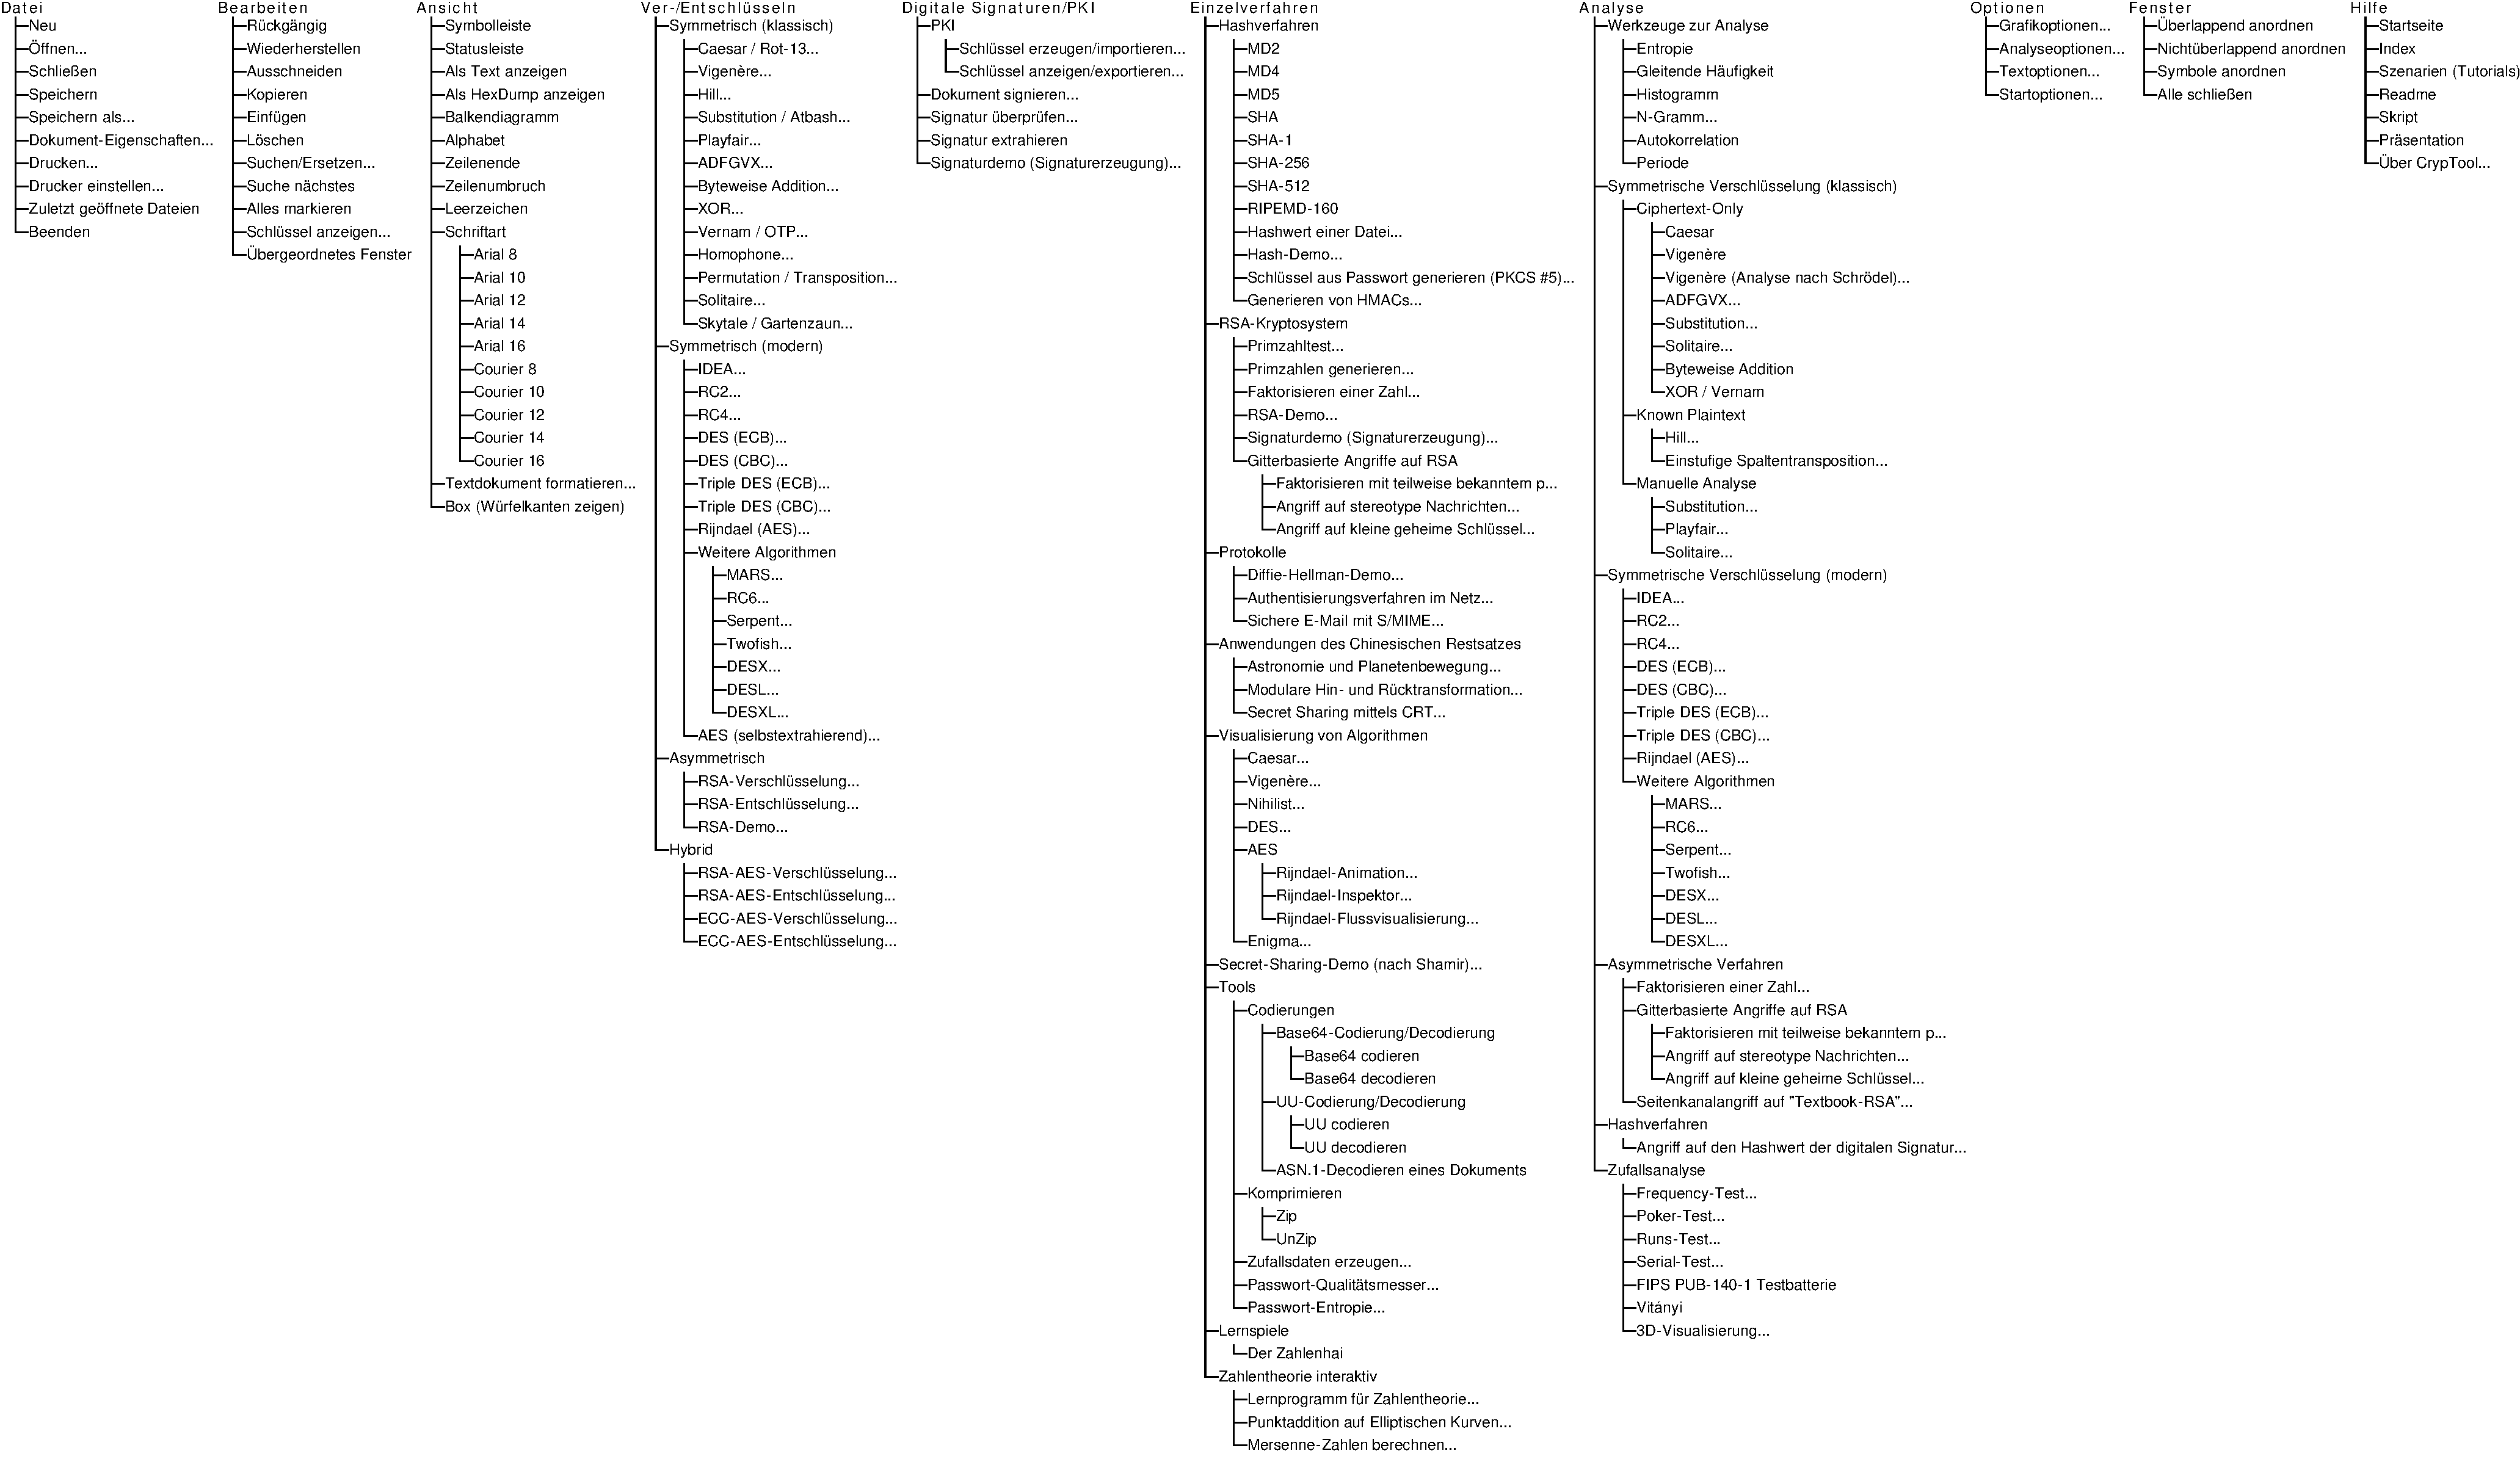
\includegraphics[scale=0.35, angle=270]
                {figures/CT1-menutree-de}
%viewport=rand-links? rand-unten breite hoehe [bezogen auf querformat]
%}
\hypertarget{appendix-figure-menu-overview-CT1}{}
\caption{Komplette �bersicht �ber den Men�-Baum von CT1 (CrypTool 1.4.31)} 
\label{appendix-figure-menu-overview-CT1}
\end{center}
\end{figure}
\clearpage




%--------------------------------------------------------------------
\newpage
%\enlargethispage{1cm}
\hypertarget{appendix-template-overview-CT2}{}
\section{CrypTool-2-Vorlagen}
\label{s:appendix-template-overview-CT2}

\noindent Dieser Anhang enth�lt auf den folgenden Seiten den Baum
mit allen Vorlagen in CrypTool 2\index{CrypTool 2}.\footnote{%
  Weitere Informationen zu CT2 finden Sie auf:
  \url{http://www.cryptool.org/de/ct2-documentation-de}
}

\noindent Beim Start von CT2 �ffnet sich das Startcenter.

%\clearpage
\begin{figure}[hb]
\begin{center}
%\vspace{-30pt}
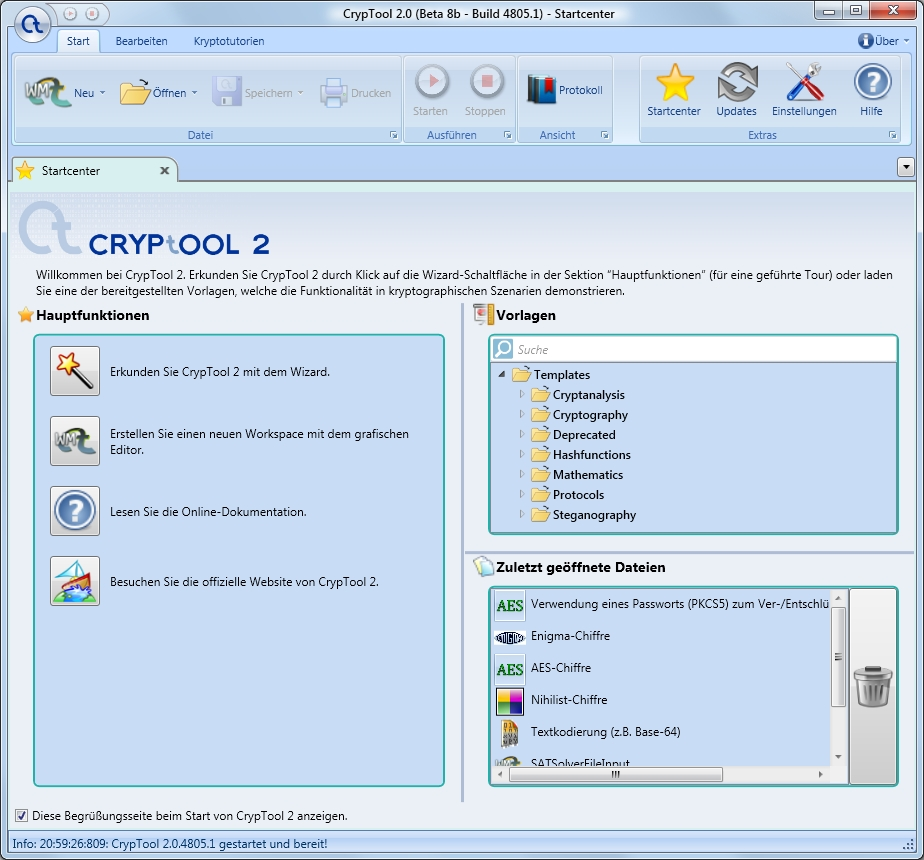
\includegraphics[scale=0.45, angle=0] {figures/CT2-Startcenter-de}
\hypertarget{Welcome-CT2}{}
\caption{Startcenter in CT2 (Beta 8b, Mai 2012)} 
\label{Welcome-Screenshot-CT2}
\end{center}
\end{figure}
%\clearpage

\noindent Darin hat man die Auswahl, die Funktionalit�t auf drei verschiedenen Wegen aufzurufen:
\begin{itemize}
   \item den Wizard: Er leitet einen gef�hrt zu den Funktionen.
   \item die Arbeitsfl�che, auf der man die Komponenten anhand der visuellen Programmierung\index{Visuelle Programmierung} selbst zusammenstellen kann.
   \item den Vorlagen-Baum, aus dem man fertige Workflows ausw�hlen kann.
 \end{itemize}

Der Wizard stellt Fragen zu dem gew�nschten Szenario (z.B. Base64-Codierung) und f�hrt einen dann zu den Funktionen. Das gew�hlte Szeanrio mit den eigenen Eingaben kann man anschlie�end auch als Vorlage abspeichern.

Auf die leere Arbeitsfl�che kann man aus der linken Navigationsleiste alle Komponenten ziehen und diese dann wie gew�nscht miteinander verbinden. Die implementierte Krypto-Funktionalit�t steckt vor allem in diesen Komponenten (z.B. Enigma, AES).

Im Vorlagen-Baum gibt es zu jeder Komponente mindestens eine Vorlage. Die angebotenen Vorlagen enthalten sofort lauff�hige komplette Workflows. Wenn man z.B. in der Vorlage zu AES seine Eingaben �ndert, sieht man dynamisch und sofort, wie sich Ausgaben entsprechend �ndern (wie z.B. durch Padding ein Block hinzukommt, wie sich das Chaining auswirkt, ...).

\clearpage
\begin{figure}[hb]
\begin{center}
\vspace{-30pt}
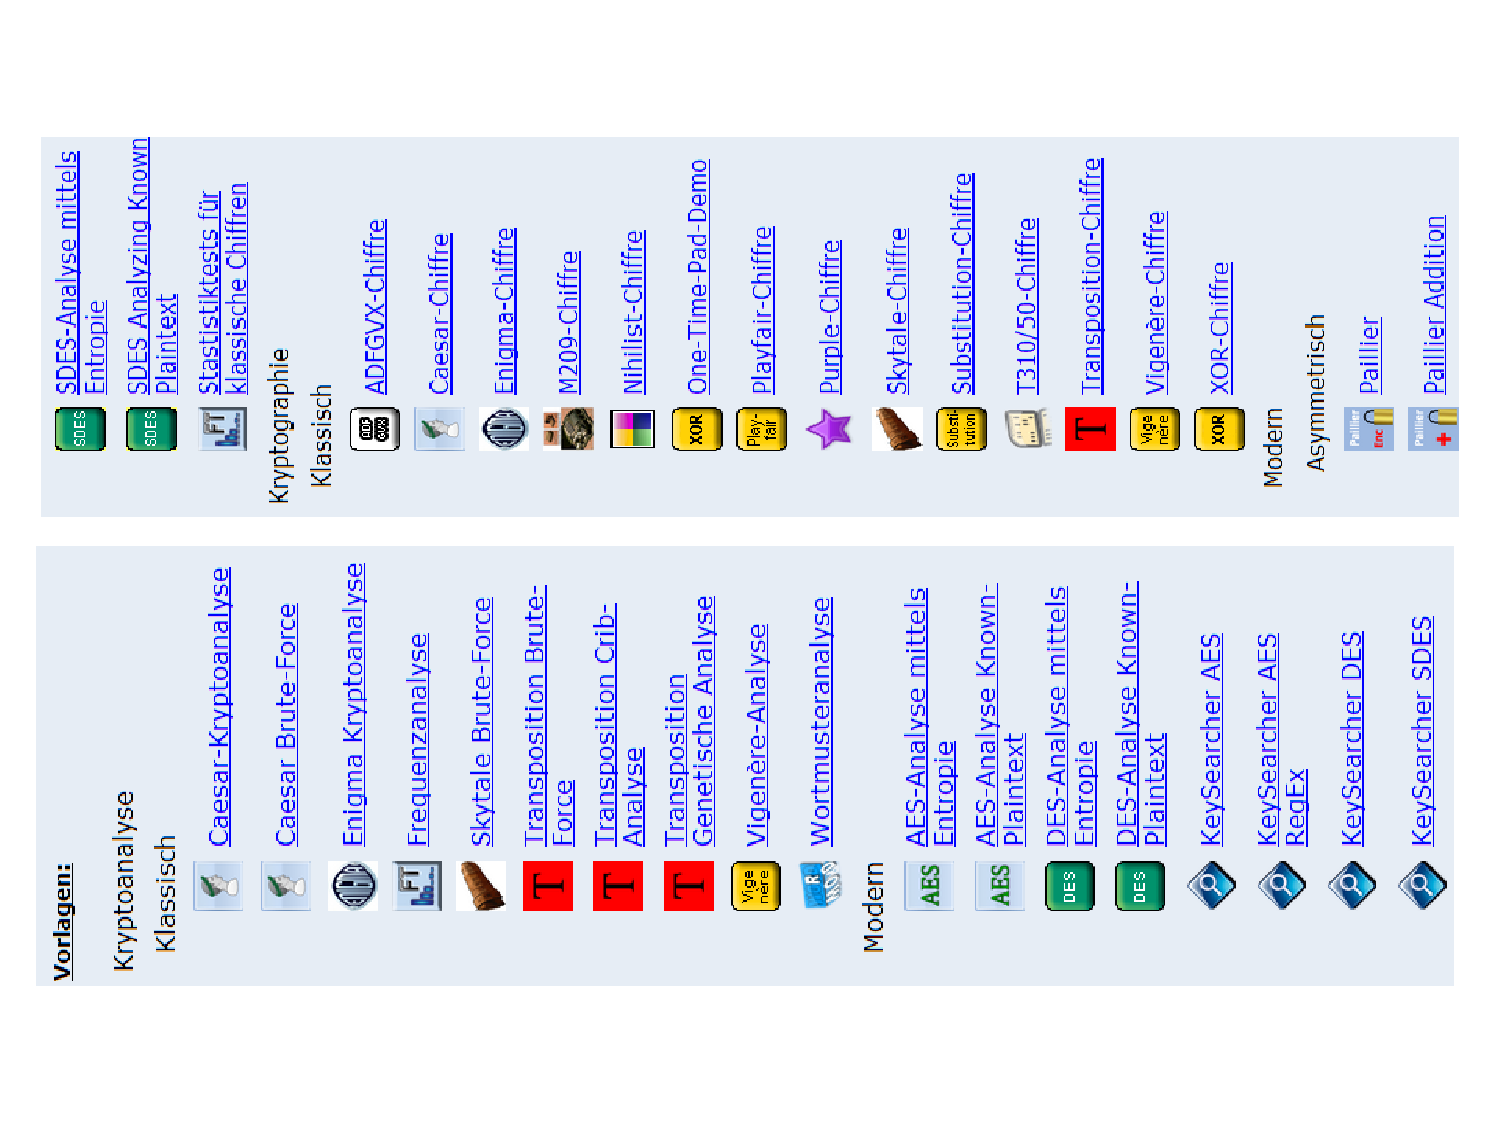
\includegraphics[scale=0.8, angle=270]
                {figures/CT2-templatetree-de-1}
\hypertarget{appendix-figure-template-overview-CT2}{}
\caption{Screenshot �ber den Template-Baum von CT2 (NB4882.1, Juli 2012), Teil 1} 
\label{appendix-figure-template-overview-CT2}
% \hypertarget{appendix-figure-template-overview-CT2}{}
\end{center}
\end{figure}
\clearpage





%--------------------------------------------------------------------
\newpage
%\enlargethispage{1cm}
\hypertarget{appendix-function-overview-JCT}{}
\section{JCrypTool-Funktionen}
\label{s:appendix-function-overview-JCT}

\noindent Dieser Anhang enth�lt auf den folgenden Seiten eine Liste aller
Funktionen in JCrypTool\index{JCrypTool}.\footnote{%
  Weitere Informationen zu JCT finden Sie auf:
  \url{http://www.cryptool.org/de/jct-machmit-de} \\
  Die Liste wurde mit Hilfe der CT-Portal-Webseite gewonnen.}

\noindent Beim ersten Start von JCT �ffnet sich das Willkommen-Fenster.

%\clearpage
\begin{figure}[hb]
\begin{center}
%\vspace{-30pt}
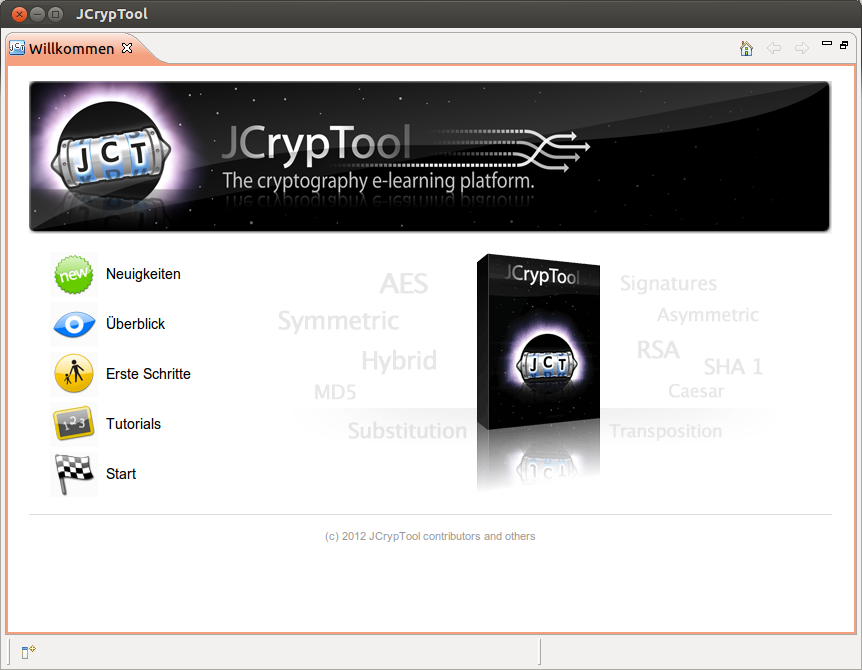
\includegraphics[scale=0.45, angle=0] {figures/JCT-Welcome-DE}
\hypertarget{Welcome-Screenshot-JCT}{}
\caption{Willkommen-Fenster in JCT (RC6, Juli 2012)} 
\label{Welcome-Screenshot-JCT}
\end{center}
\end{figure}
%\clearpage
Mit Klick auf ``Start'' kann man die verschiedenen Funktionen direkt nutzen.
Die in JCT implementierten Funktionen werden �ber zwei unterschiedliche Perspektiven angeboten:
\begin{itemize}
   \item Standard-Perspektive
   \item Funktional-Perspektive
 \end{itemize}

Alle Funktionen in der {\bf Standard-Perspektive} finden sich sowohl in den Men�s als
auch in der ``Krypto-Explorer'' genannten Navigationsleiste (rechts). Die Standard-Perspektive enth�lt alle wichtigen Verfahren (wie z.B. die klassische Transposition oder der moderne AES)  und viele Visualisierungen (z.B. Diffie-Hellman-Schl�sselaustausch oder Berechnungen auf Elliptischen Kurven).

Alle Funktionen der {\bf Funktional-Perspektive} finden sich in der ``Algorithmen'' genannten Navigationsleiste (in dieser Perspektive ebenfalls rechts). Die Funktional-Perspektive enth�lt alle Detaileinstellungen der verschiedenen Algorithmen und bietet insbesondere auch Algorithmen aus dem Bereich des Post-Quantum-Computings\index{Post-Quantum-Computing} an.

\clearpage
\begin{figure}[hb]
\begin{center}
\vspace{-30pt}
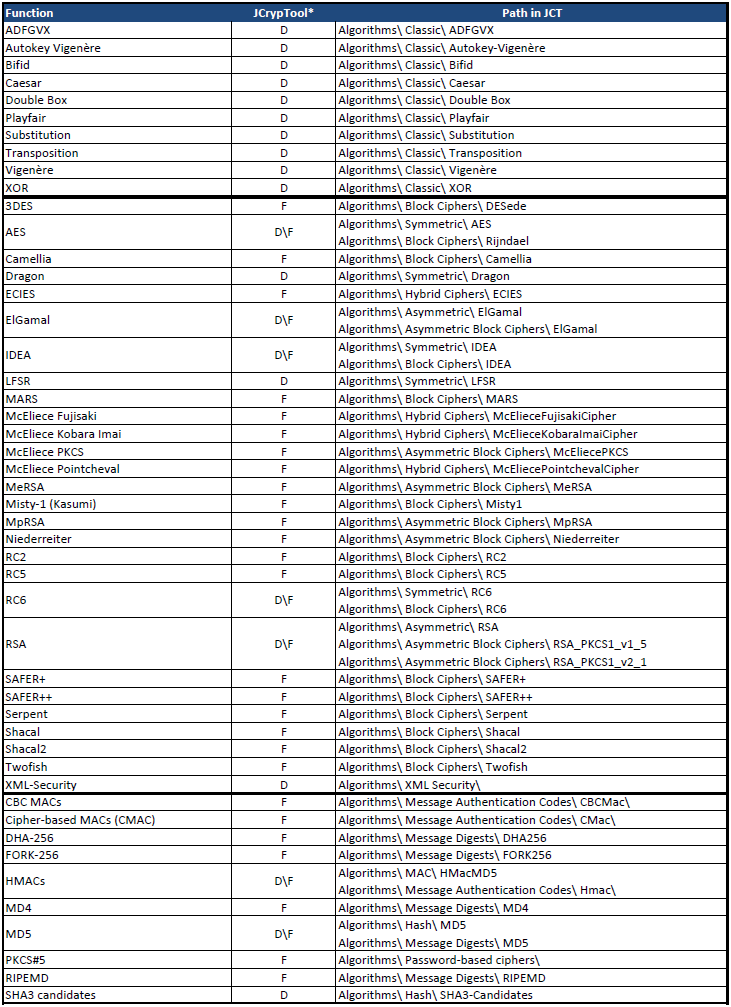
\includegraphics[scale=0.8, angle=0] {figures/JCT-functions-de-1}
\hypertarget{functions-overview-1-JCT}{}
\caption{Screenshot zu den Funktionen in JCT (RC6, Juli 2012), Teil 1} 
\label{functions-overview-1-JCT}
\end{center}
\end{figure}
\clearpage

\clearpage
\begin{figure}[hb]
\begin{center}
\vspace{-30pt}
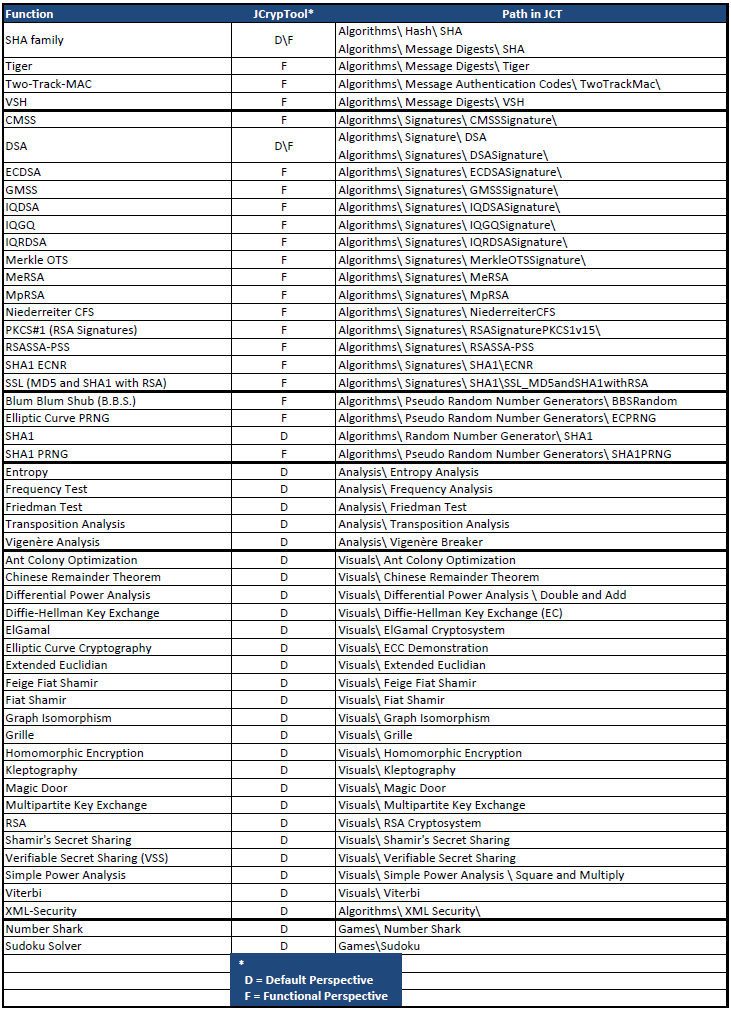
\includegraphics[scale=0.8, angle=0] {figures/JCT-functions-de-2}
\hypertarget{functions-overview-2-JCT}{}
\caption{Screenshot zu den Funktionen in JCT (RC6, Juli 2012), Teil 2} 
\label{functions-overview-2-JCT}
\end{center}
\end{figure}
\clearpage





%--------------------------------------------------------------------
\newpage
%\enlargethispage{1cm}
\hypertarget{appendix-function-overview-CTO}{}
\section{CrypTool-Online-Funktionen}
\label{s:appendix-function-overview-CTO}

\noindent Dieser Anhang enth�lt eine Liste aller
Funktionen in CrypTool-Online (CTO)\index{CrypTool-Online}.\footnote{%
  Weitere Informationen zu CTO finden Sie auf:
  \url{www.cryptool-online.org} \\
  Die Liste wurde mit Hilfe der Funktionsliste auf der CT-Portal-Webseite gewonnen:\\
  \url{http://www.cryptool.org/ctp-documentation-en/ctp-functions-en}}


%\noindent Die Einstiegsseite von CTO sieht so aus:
%\clearpage
%\begin{figure}[hb]
%\begin{center}
%\vspace{-30pt}
%\includegraphics[scale=0.45, angle=0] {figures/CTO-Welcome-DE}
%\hypertarget{Welcome-Screenshot-CTO}{}
%\caption{Einstiegsseite in CrypTool-Online (November 2012)} 
%\label{Welcome-Screenshot-CTO}
%\end{center}
%\end{figure}
%\clearpage


\noindent Der folgende Screenshot zeigt die auf CTO implementierten
Krypto-Funktionen:
\clearpage
\begin{figure}[hb]
\begin{center}
\vspace{-30pt}
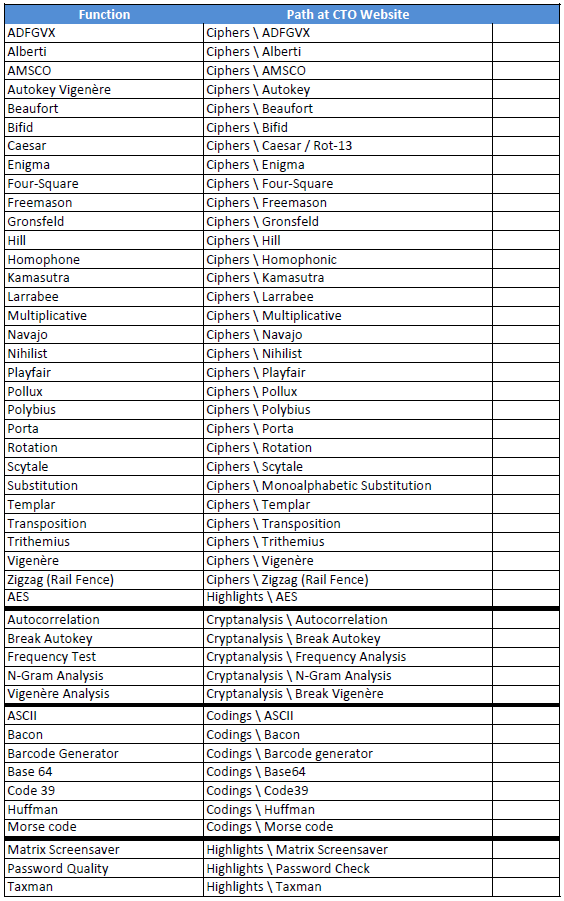
\includegraphics[scale=0.8, angle=0] {figures/CTO-functions-de-1}
\hypertarget{functions-overview-1-CTO}{}
\caption{Screenshot zu den Funktionen in CTO (November 2012)} 
\label{functions-overview-1-CTO}
\end{center}
\end{figure}
\clearpage

%\clearpage
%\begin{figure}[hb]
%\begin{center}
%\vspace{-30pt}
%\includegraphics[scale=0.8, angle=0] {figures/CTO-functions-de-2}
%\hypertarget{functions-overview-2-CTO}{}
%\caption{Screenshot zu den Funktionen in CTO (November 2012), Teil 2} 
%\label{functions-overview-2-CTO}
%\end{center}
%\end{figure}
%\clearpage


  \renewcommand{\CTBChapName}{(Appendix LearnTool)}  % $Id:
% !Mode:: "TeX:DE"    % Setting document mode and submode for WinEdt
% ..............................................................................
%             F I L M E  +  R O M A N E
% ~~~~~~~~~~~~~~~~~~~~~~~~~~~~~~~~~~~~~~~~~~~~~~~~~~~~~~~~~~~~~~~~~~~~~~~~~~~~~~
%
% Consider to add next time:
%  - Filme: Matrix, Tron, Echelon Verschw�rung, ...
%  - B�cher: xxx, ...
% ~~~~~~~~~~~~~~~~~~~~~~~~~~~~~~~~~~~~~~~~~~~~~~~~~~~~~~~~~~~~~~~~~~~~~~~~~~~~~~


\begin{bibunit}[babalpha] %% alpha: Chapter bibliography shows authors abbreviation

\newpage
\hypertarget{appendix-movies}{}
\section{Filme und belletristische Literatur mit Bezug zur Kryptographie}
\label{s:appendix-movies}
% {\bf Filme und Literatur mit Bezug zur Kryptographie} (siehe Anhang \ref{s:appendix-movies})
\index{Filme}
\index{Literatur}


Kryptographische Verfahren -- sowohl klassische wie moderne -- fanden auch
Eingang in die Literatur und in Filme. In manchen Medien werden diese nur
erw�hnt und sind reine Beigabe, in anderen sind sie tragend und werden
genau erl�utert, und manchmal ist die Rahmenhandlung nur dazu da, dieses
Wissen motivierend zu transportieren. Anbei der Beginn eines �berblicks.

% --------------------------------------------------------------------------
\subsection{F�r Erwachsene und Jugendliche}
\label{s:Light-fiction-for-grownups}

%be_2005: Hatte zuerst \begin{thebibliography}{99999} und \bibitem[... ,
%         aber dann wurde immer der feste Titel "Literatur" bzw. "References"
%         geschrieben und wir fanden keine M�glichkeit, ihn weg zu bekommen.
%         L�sung: Stattdessen \begin{description} \item[...


\begin{description}

\item[\textrm{[Poe1843]}] \index{Poe 1843}
    Edgar Allan Poe\index{Poe, Edgar Allan}, \\
    {\em Der Goldk�fer}, 1843.\footnote{%
        Siehe \url{https://de.wikipedia.org/wiki/Der_Goldk%C3%A4fer}.

	Eine didaktisch aufbereitete Beschreibung zum Einsatz im Schulunterricht findet
        sich in Teil 1 der Artikelserie {\em RSA \& Co. in der Schule:
        Moderne Kryptologie, alte Mathematik, raffinierte Protokolle}.
        Siehe \cite{Witten1998}, S. 52 ff (\glqq Das Gold des Gehenkten\grqq).
	\index{RSA \& Co. in der Schule}

	Alle Materialien zu der Goldk�fer-Unterrichtsstunde (oder Doppelstunde)
	finden sich unter \url{http://www.informatik-im-kontext.de/} via
	\glqq E-Mail (nur?) f�r Dich\grqq~=> \glqq Vertraulichkeit mit Verschl�sselungsverfahren\grqq.
	% In den Materialien wird ein erprobter generischer Gang zu RSA pr�sentiert:
	% Monoalphabetische Verschl�sselung (Goldk�fer) => Knacken durch H�ufigkeitsanalyse
	% => polyalphabetische Verschl�sselung => Knacken durch Bestimmung der Schl�ssell�nge (Kasiski, Friedman)
	% => One-Time-Pad als beweisbar sicheres Verschl�sselungsverfahren
	% => Problem des Schl�sselmanagments => asymmetrische Kryptographie (Diffie, Hellman, Merkle, RSA).

	Poe war nicht nur ein bekannter -- in seiner Heimat Amerika zun�chst
	verkannter -- Schriftsteller und Erfinder des Kriminalromans,
	%% (�Der Doppelmord in der Rue Morgue�, s. https://de.wikipedia.org/wiki/Edgar_Allan_Poe,
	%% https://de.wikipedia.org/wiki/Der_Doppelmord_in_der_Rue_Morgue)
	sondern auch ein begabter Kryptologe. Die Geschichte dazu wird auch in dem
	Krypto-Buch {\em Verschl�sselte Botschaften} \cite{Kippenhahn1997}
	erz�hlt.
    }\\
    Diese Kurzgeschichte erschien in Deutsch z.B. in der illustrierten und
    mit Kommentaren in den Marginalspalten versehenen Ausgabe "`Der Goldk�fer
    und andere Erz�hlungen"', Gerstenbergs visuelle Weltliteratur,
    Gerstenberg Verlag, Hildesheim, 2002.\\
    In dieser Kurzgeschichte beschreibt Poe als Ich-Erz�hler seine
    Bekanntschaft mit dem sonderbaren Legrand. Mit Hilfe eines an der
    K�ste Neuenglands gefundenen Goldk�fers, einem alten Pergament und
    den Dechiffrierk�nsten von Legrand finden Sie den sagenhaften Schatz
    von Kapit�n Kidd.\\
    Die Geheimschrift besteht aus 203 kryptischen Zeichen und erweist sich
    als allgemeine monoalphabetische Substitutions-Chiffre (vgl.
    Kapitel~\ref{monoalphabeticSubstitutionCiphers}). Ihre schrittweise
    Dechiffrie"-rung durch semantische und syntaktische Analyse
    (H�ufigkeit der einzelnen Buchstaben in englischen Texten)
    wird in der Geschichte ausf�hrlich erl�utert.\footnote{%
      Teil der oben genannten Unterrichtsmaterialien ist auch ein Python-Programm.\index{Python}
      %% Au�erdem gibt es eine schrittweise L�sung des Gold-Bug-Kryptogramms,
      %% das vor einigen Jahren Wittens Frau in Standard-HTML schrieb.
      Damit l�sst sich das Kryptogramm mit Python {\em und} mit SageMath\index{SageMath}
      entschl�sseln.
      Siehe das Code-Beispiel in \ref{s:appendix-Code-for-light-fiction-books}.
      % \ref{Lit_Python-sample_Gold-bug}  Hier druckt er "A.1" ?
    }\\
    Der Entschl�sseler Legrand sagt darin (S. 39) den ber�hmten Satz:
    "`Und es ist wohl sehr zu bezweifeln, ob menschlicher Scharfsinn
    ein R�tsel ersinnen kann, das menschlicher Scharfsinn bei
    entsprechender Hingabe nicht wieder zu l�sen vermag."'\\
    % D: Poe: 1809-1849, "Vater des Kriminalromans", er schloss Wetten ab,
    % dass er alle verschl�sselten Botschaften, die ihm Freunde und Leser
    % vorlegten, im Handumdrehen entschl�sseln k�nne. Gutes Gesp�r durch
    % viel �bung.
    % E: Poe, 1809-1849 was named "Father of the crime novel". He claimed,
    % that he will be able to decrypt any cipher sent to him by friends or
    % readers.
    %
    % Originalausgabe dieser illustrierten Ausgabe: "Le scarab�e d'or et
    %                           autre nouvelles", Gallimard, Paris, 1998.
    % In "Der Goldk�fer" wird detailliert beschrieben, wie der verarmte
    % Hugenotte William Legrand in South Carolina die monoalphabetische
    % Geheimschrift des Piratenkapit�ns Kidd knackt, die zu einem
    % sagenhaften Schatz f�hrt.


\item[\textrm{[Verne1885]}] \index{Verne 1885}
    Jules Verne\index{Verne, Jules}, \\
    {\em Mathias Sandorf}, 1885. \\
    Dies ist einer der bekanntesten Romane des franz�sischen Schriftstellers
    Jules Verne (1828-1905), der auch als "`Vater der Science Fiction"'
    bezeichnet wurde.\\
    Erz�hlt wird die spannende Geschichte des Freiheitsk�mpfers Graf
    Sandorf, der an die Polizei verraten wird, aber schlie�lich fliehen
    kann.\\
    M�glich wurde der Verrat nur, weil seine Feinde eine Geheimbotschaft an
    ihn abfangen und entschl�sseln konnten. Dazu ben�tigten sie eine
    besondere Schablone, die sie ihm stahlen. Diese Schablone bestand aus
    einem quadratischen St�ck Karton mit 6x6 K�stchen, wovon 1/4, also neun,
    ausgeschnitten waren (vgl. die
    \hyperlink{turning-grille-cipher}{Flei�ner-Schablone}
    in Kapitel~\ref{introsamplesTranspositionCiphers}).\\


    % Gefunden in: CRYPTO-GRAM, January 15, 2007, by Bruce Schneier
\item[\textrm{[Kipling1901]}] \index{Kipling 1901}
    Rudyard Kipling\index{Kipling, Rudyard}, \\
    {\em Kim}, 1901. \\
    Dieser Roman wird in der Besprechung von Rob Slade%
    \footnote{Siehe
      % \href{http://catless.ncl.ac.uk/Risks/24.49.html\#subj12} %% \ vor # n�tig !
        \url{http://catless.ncl.ac.uk/Risks/24.49.html#subj12}.
    }
    folgenderma�en beschrieben:
    "`Kipling packte viele Informationen und Konzepte in seine Geschichten.
    In "`Kim"' geht es um das gro�e "`Spiel"' Spionage und Bespitzelung.
    Schon auf den ersten 20 Seite finden sich Authentisierung �ber Besitz,
    Denial of Service, Sich-f�r-jemand-anderen-Ausgeben (Impersonation),
    Heimlichkeit, Maskerade, Rollen-basierte Autorisierung (mit
    Ad-hoc-Authentisierung durch Wissen), Abh�ren, und Vertrauen basierend
    auf Datenintegrit�t.
    Sp�ter kommen noch Contingency Planning gegen Diebstahl und
    Kryptographie mit Schl�sselwechsel hinzu."'\\
    Das Copyright des Buches ist abgelaufen.%
    \footnote{Sie k�nnen es lesen unter:\\
          \url{http://whitewolf.newcastle.edu.au/words/authors/K/KiplingRudyard/prose/Kim/index.html},\\
          \url{http://kipling.thefreelibrary.com/Kim} oder\\
          \url{http://www.readprint.com/work-935/Rudyard-Kipling}.
    }\\


\item[\textrm{[Doyle1905]}] \index{Doyle 1905}
    Arthur Conan Doyle\index{Doyle, Sir Arthur Conan}, \\
    {\em Die tanzenden M�nnchen}, 1905. \\
    In der Sherlock-Holmes-Erz�hlung {\em Die tanzenden M�nnchen}
    (erschienen erstmals 1903 im "`Strand Magazine"', und dann 1905 im
    Sammelband "`Die R�ckkehr des Sherlock Holmes"' erstmals in Buchform)
    wird Sherlock Holmes mit einer Geheimschrift konfrontiert, die zun�chst
    wie eine harmlose Kinderzeichnung aussieht. \\
    Sie erweist sich als monoalphabetische Substitutions-Chiffre (vgl.
    Kapitel~\ref{monoalphabeticSubstitutionCiphers}) des Verbrechers Abe
    Slaney. Holmes knackt die Geheimschrift mittels H�ufigkeitsanaly"-se.\\


\item[\textrm{[Sayers1932]}] \index{Sayers 1932}
    Dorothy L. Sayers, \\
    {\em Zur fraglichen Stunde und Der Fund in den Teufelsklippen
    (Orginaltitel: Have his carcase)}, Harper, 1932 \\
    (Erste dt. �bersetzung {\em Mein Hobby: Mord} bei A. Scherz, 1964; \\
    dann {\em Der Fund in den Teufelsklippen} bei Rainer Wunderlich-Verlag,
    1974;\\
    Neu�bersetzung 1980 im Rowohlt-Verlag). \\
    In diesem Roman findet die Schriftstellerin Harriet Vane eine Leiche
    am Strand und die Polizei h�lt den Tod f�r einen Selbstmord.
    Doch Harriet Vane und der elegante Amateurdetektiv Lord Peter Wimsey
    kl�ren in diesem zweiten von Sayers's ber�hmten Harriet Vane's
    Geschichten den widerlichen Mord auf. \\
    Dazu ist ein Chiffrat zu l�sen. Erstaunlicherweise beschreibt der
    Roman nicht nur detailliert die Playfair-Chiffre, sondern auch deren
    Kryptoanalyse (vgl. \hyperlink{playfair}{Playfair}
    in Kapitel~\ref{polygraphicSubstitutionCiphers}).\\


\item[\textrm{[Simmel1970]}] \index{Simmel 1970}
    Johannes Mario Simmel, \\
    {\em Und Jimmy ging zum Regenbogen}, Knaur Verlag, 1970. \\
    Der Roman spielt zwischen 1938 und
    1969 in Wien. Der Held Manuel Aranda deckt -- von mehreren Geheimdiensten
    verfolgt -- im Laufe der Handlung St�ck f�r St�ck die Vergangenheit seines
    ermordeten Vaters auf. Ein wichtiger Mosaikstein ist dabei ein
    verschl�sseltes Manuskript, das in Kapitel 33 entschl�ssselt wird.
    Im Roman wird der Code als ein
    "`f�nfundzwanzigfacher Caesar Code"' beschrieben, tats�chlich ist es eine
    Vigen�re-Chiffre mit einem 25 Buchstaben langen Schl�ssel. \\
    Das Buch wurde 1971 verfilmt.\\


\item[\textrm{[Crichton1988]}] \index{Crichton 1988}
    Michael Crichton, \\
    {\em Die Gedanken des B�sen (Orginaltitel: Sphere)}, Rororo, 1988. \\
    Ein Team verschiedener Wissenschaftler wird auf den Meeresgrund geschickt,
    um ein 900~m langes hoch entwickeltes Raumschiff zu untersuchen. Die
    Eigenheiten und psychischen Probleme der Forscher treten durch lebensbedrohliche
    Ereignisse und ihr Abgeschnittensein von oben immer mehr in den Vordergrund.
    Es gibt viele R�tsel: Das Raumschiff liegt schon 300 Jahre da, es hat
    englische Beschriftungen, es f�hrt scheinbar ein Eigenleben, die menschliche
    Vorstellungskraft materialisiert sich. Unter anderem erscheint auf dem
    Bildschirm ein im Buch vollst�ndig abgedruckter Code, der von dem genialen
    Mathematiker Harry entschl�sselt werden kann: ein einfacher spiralenf�rmiger
    Ersetzungscode.\\


\item[\textrm{[Seed1990]}] \index{Seed 1990}
    Regie Paul Seed (Paul Lessac), \\
    {\em Das Kartenhaus (Orginaltitel: House of Cards)}, 1990 (dt. 1992). \\
    In diesem Film versucht Ruth, hinter das Geheimnis zu kommen, das ihre
    Tochter verstummen lie�. Hierin unterhalten sich Autisten mit Hilfe von
    5- und 6-stelligen Primzahlen (siehe
    Kapitel~\ref{Chapter_Primes}).
    Nach �ber eine Stunde kommen im Film die folgenden beiden (nicht
    entschl�sselten) Primzahlfolgen vor:
%  \vskip -30pt  %be_2005 Bewirkt anscheinend nichts -- Abstand etwas zu gro�.
    \begin{center}
    $21.383, \;\;176.081, \;\;18.199, \;\;113.933, \;\;150.377, \;\;304.523, \;\;113.933$\\
    $193.877, \;\;737.683, \;\;117.881, \;\;193.877$
    \end{center}
    \vskip +10 pt   % da "\\" hier nicht geht!


\item[\textrm{[Robinson1992]}] \index{Robinson 1992}
    Regie Phil Alden Robinson, \\
    {\em Sneakers - Die Lautlosen (Orginaltitel: Sneakers)},
    Universal Pictures Film, 1992. \\
    In diesem Film versuchen die "`Sneakers"' (Computerfreaks um ihren Boss
    Martin Bishop), den "`B�sen"' das Dechiffrierungsprogramm SETEC abzujagen.
    SETEC wurde von einem genialen Mathematiker vor seinem gewaltsamen Tod
    erfunden und kann alle Geheimcodes dieser Welt entschl�sseln.\\
    In dem Film wird das Verfahren nicht beschrieben%
    \footnote{
       An dem Film hatte Leonard Adleman (das "`A"' von RSA) als mathematischer
       Berater mitgearbeitet. Die recht lustige Geschichte �ber seine Mitwirkung
       bei Sneakers beschreibt er selbst auf seiner Homepage unter
       \url{http://www.usc.edu/dept/molecular-science/fm-sneakers.htm}.
       Man kann man davon ausgehen, dass es sich bei dem �berall benutzten
       Verschl�sselungsverfahren um RSA handelt.
       In dem Chip ist demnach ein bis dahin unbekanntes, schnelles
       Faktorisierungsverfahren\index{Faktorisierung} implementiert.
    }.\\


\item[\textrm{[Baldacci1997]}] \index{Baldacci 1997}
    David Baldacci, \\
    {\em Das Labyrinth. Total Control}, L�bbe, 1997. \\
    Jason Archer, Direktor einer Technologie-Firma, verschwindet pl�tzlich.
    Seine Frau Sidney Archer versucht, den Grund seines pl�tzlichen Todes
    herauszufinden, und entdeckt, wie das Finanzsystem missbraucht wird und
    dass die reale Macht bei denen mit dem meisten Geld liegt. Hier helfen
    dann auch gute Passworte nicht...\\


\item[\textrm{[Natali1997]}] \index{Natali 1997}
    Regie Vincenzo Natali, \\
    {\em Cube (Orginaltitel: Sneakers)},
    Mehra Meh Film, 1997. \\
    In diesem kanadischen Low-Budget-Film finden sich 7 sehr unterschiedliche
    Personen in einem endlos scheinenden Labyrinth von w�rfelartigen R�umen.\\
    Die Personen wollen nach drau�en, m�ssen dazu aber die R�ume durchqueren,
    von denen manche t�dliche Fallen darstellen. Um herauszufinden, welche
    R�ume gef�hrlich sind, spielt Mathematik eine entscheidende Rolle: Jeder
    Raum hat am Eingang eine Folge von 3 mal 3 Ziffern. Zuerst nehmen
    sie an, dass alle R�ume Fallen sind, wo wenigstens eine der 3 Zahlen eine
    Primzahl ist. Sp�ter stellt sich heraus, dass auch alle diejenigen R�ume
    Fallen sind, bei denen eine der 3 Zahlen eine Potenz von genau einer
    Primzahl ist (Fallen sind also $p^n$, z.B. $128=2^7$ oder
    $101 = 101^1 = prim$, aber nicht $517 = 11*47$).\\


\item[\textrm{[Becker1998]}] \index{Becker 1998}
    Regie Harold Becker, \\
    {\em Das Mercury Puzzle (Orginaltitel: Mercury Rising)},
    Universal Pictures Film, 1998. \\
    Die NSA hat einen neuen Code entwickelt, der angeblich weder von Menschen
    noch von Computern geknackt werden kann. Um die Zuverl�ssigkeit zu testen,
    verstecken die Programmierer eine damit verschl�sselte Botschaft in
    einem R�tselheft.\\
    Simon, eine neunj�hriger autistischer Junge, knackt den Code.
    Statt den Code zu fixen, schickt ihm ein Sicherheitsbeamter einen Killer.
    Der FBI-Agent Art Jeffries (Bruce Willis) besch�tzt den Jungen und
    stellt den Killern eine Falle.\\
    Das Chiffrier-Verfahren wird nicht beschrieben.\\


\item[\textrm{[Brown1998]}] \index{Brown 1998}
    Dan Brown, \\
    {\em Diabolus (Orginaltitel: Digital Fortress)}, L�bbe, 2005. \\
    Dan Browns erster Roman "`The Digital Fortress"' erschien 1998 als E-Book,
    blieb jedoch damals weitgehend erfolglos.\\
    Die National Security Agency (NSA) hat f�r mehrere Milliarden US-Dollar
    einen gewaltigen Computer gebaut, mit dem sie in der Lage ist, auch nach
    modernsten Verfahren verschl�sselte Meldungen (nat�rlich nur die von
    Terroristen und Verbrechern) innerhalb weniger Minuten zu entziffern.\\
    Ein abtr�nniger Angestellter erfindet einen unbrechbaren Code und
    sein Computerprogramm Diabolus zwingt damit den Supercomputer zu
    selbstzerst�rerischen Rechenoperationen. Der Plot, in dem auch die
    sch�ne Computerexpertin Susan Fletcher eine Rolle spielt, ist ziemlich
    vorhersehbar.\\
    Die Idee, dass die NSA oder andere Geheimdienste jeden Code knacken
    k�nnen, wurde schon von mehreren Autoren behandelt: Hier hat der
    Supercomputer 3 Millionen Prozessoren -- trotzdem ist es aus heutiger
    Sicht damit auch nicht ann�herungsweise m�glich, diese modernen Codes
    zu knacken.\\


\item[\textrm{[Elsner1999]}] \index{Elsner 1999}
    Dr.~C.~Elsner, \\
    {\em Der Dialog der Schwestern}, c't, Heise-Verlag, 1999. \\
    In dieser Geschichte, die dem CrypTool-Paket\index{CrypTool} als PDF-Datei
    beigelegt ist, unterhalten sich die Heldinnen vertraulich mit einer
    Variante des RSA-Verfahrens (vgl. Kapitel~\ref{rsabeweis} ff.).
    Sie befinden sich in einem Irrenhaus unter st�ndiger Bewachung.\\


\item[\textrm{[Stephenson1999]}] \index{Stephenson 1999}
    Neal Stephenson, \\
    {\em Cryptonomicon}, Harper, 1999. \\
    Der sehr dicke Roman besch�ftigt sich mit Kryptographie sowohl im
    zweiten Weltkrieg als auch in der Gegenwart.
    Die zwei Helden aus den 40er-Jahren sind der gl�nzende Mathematiker und
    Kryptoanalytiker Lawrence Waterhouse, und der �bereifrige,
    morphiums�chtige Bobby Shaftoe von den US-Marines.
    Sie geh�ren zum Sonderkommando 2702, einer Alliiertengruppe, die
    versucht, die gegnerischen Kommunikationscodes zu knacken und dabei
    ihre eigene Existenz geheim zu halten. \\
    In der Gegenwartshandlung tun sich die Enkel der Weltkriegshelden -- der
    Programmierfreak Randy Waterhouse und die sch�ne Amy Shaftoe -- zusammen. \\
    Cryptonomicon ist f�r nicht-technische Leser teilweise schwierig zu
    lesen. Mehrere Seiten erkl�ren detailliert Konzepte der Kryptographie.
    Stephenson legt eine ausf�hrliche Beschreibung der Solitaire-Chiffre
    (siehe Kapitel~\ref{Further-PaP-methods}) bei, ein
    Papier- und Bleistiftverfahren\index{Papier- und Bleistiftverfahren},
    das von Bruce Schneier entwickelt wurde und im
    Roman "`Pontifex"' genannt wird. Ein anderer, moderner Algorithmus
    namens "`Arethusa"' wird dagegen nicht offengelegt.\\


\item[\textrm{[Elsner2001]}] \index{Elsner 2001}
    Dr.~C.~Elsner, \nopagebreak\\
    {\em Das Chinesische Labyrinth}, c't, Heise-Verlag, 2001. \\
    In dieser Geschichte, die dem CrypTool-Paket\index{CrypTool} als PDF-Datei
    beigelegt ist, muss Marco Polo in einem Wettbewerb Probleme aus der
    Zahlentheorie l�sen, um Berater des gro�en Khan zu werden. Alle L�sungen
    sind angef�gt und erl�utert.\\


\item[\textrm{[Colfer2001]}] \index{Colfer 2001}
    Eoin Colfer, \\
    {\em Artemis Fowl}, List-Verlag, 2001. \\
    In diesem Jugendbuch gelangt der junge Artemis, ein Genie und Meisterdieb,
    an eine Kopie des streng geheimen "`Buches der Elfen"'. Nachdem er es mit
    Computerhilfe entschl�sselt hat, erf�hrt er Dinge, die kein Mensch
    erfahren d�rfte. \\
    Der Code wird in dem Buch nicht genauer beschrieben.\\


\item[\textrm{[Howard2001]}] \index{Howard 2001}
    Regie Ron Howard, \\
    {\em A Beautiful Mind}, 2001. \\
    Verfilmung der von Sylvia Nasar verfassten Biographie des
    Spieltheoretikers John Nash.
    Nachdem der brillante, aber unsoziale Mathematiker geheime kryptographische
    Arbeiten annimmt, verwandelt sich sein Leben in einen Alptraum. Sein
    unwiderstehlicher Drang, Probleme zu l�sen, gef�hrden ihn und sein
    Privatleben.
    Nash ist in seiner Vorstellungswelt ein staatstragender Codeknacker. \\
    Konkrete Angaben zur seinen Analyseverfahren werden nicht beschrieben.\\


\item[\textrm{[Apted2001]}] \index{Apted 2001}
    Regie Michael Apted, \\
    {\em Enigma -- Das Geheimnis}, 2001. \\
    Verfilmung des von Robert Harris verfassten "`historischen Romans"'
    {\em Enigma} (Hutchinson, London, 1995) �ber die ber�hmteste
    Verschl�sselungsmaschine in der Geschichte, die in
    Bletchley Park nach polnischen Vorarbeiten gebrochen wurde.
    Die Geschichte spielt 1943, als der eigentliche Erfinder Alan Turing
    schon in Amerika war. So kann der Mathematiker Tom Jericho als Hauptperson
    in einem spannenden Spionagethriller brillieren.\\
    Konkrete Angaben zu dem Analyseverfahren werden nicht gemacht.\\


\item[\textrm{[Isau2003]}] \index{Isau 1997}
    Ralf Isau, \\
    {\em Das Museum der gestohlenen Erinnerungen}, Thienemann-Verlag, 1997/2003. \\
    Ein sehr spannender, hervorragend recherchierter und doch leicht zu lesender
    Roman mit einem tiefen Hintersinn.\\
    Als die Zwillinge Oliver und Jessica von ihren Ferien zur�ckkommen, haben sie
    ihren Vater vergessen. Die Realit�t verschiebt sich und niemand scheint es zu
    bemerken. An einigen Stellen bleiben manchmal Spuren zur�ck, die man
    entziffern kann.
    Zentrum der Geschichte ist das Ischtar-Tor im Berliner Pergamon-Museum.
    Nur mit dem Scharfsinn einer irischen Professorin (die gleichzeitig
    Computerexpertin, Arch�ologin und Philologin ist), den besonderen
    Beziehungen zwischen Zwillingen und den vereinten Kr�ften der
    Computergemeinschaft kann der letzte Teil des Spruches gel�st werden.\\
    Das Buch wurde als bestes Jugendbuch ausgezeichnet und liegt in 8 Sprachen vor.\\


\item[\textrm{[Brown2003]}] \index{Brown 2003}
    Dan Brown, \\
    {\em Sakrileg (Orginaltitel: The Da Vinci Code)}, L�bbe, 2004. \\
    Der Direktor des Louvre wird in seinem Museum vor einem Gem�lde Leonardos
    ermordet aufgefunden, und der Symbolforscher Robert Langdon ger�t in eine
    Verschw�rung.\\
    Innerhalb der Handlung werden verschiedene klassische Chiffren (Substitution
    wie z.B. Caesar oder Vigen\`ere, sowie Transposition und Zahlencodes)
    angesprochen. Au�erdem klingen interessante Nebenbemerkungen �ber
    Schneier oder die Sonnenblume an.
    Der zweite Teil des Buches ist sehr von theologischen Betrachtungen
    gepr�gt. \\
    Das Buch ist einer der erfolgreichsten Romane der Welt.\\

% Rezensionen aus der Amazon.de-Redaktion:
% Bestsellerautor Dan Brown bietet mit Sakrileg erneut spannende und intelligente Unterhaltung vom Feinsten. Der Direktor des Louvre wird in seinem Museum vor einem Gem�lde Leonardos ermordet aufgefunden, und der Symbolforscher Robert Langdon ger�t ins Fadenkreuz der Polizei, war er doch mit dem Opfer just zur Tatzeit verabredet. Eine Verschw�rung ist immer noch das Sch�nste. Stimmt, wenn sie schriftstellerisch so �berzeugend und raffiniert inszeniert ist, wie es dem Amerikaner Dan Brown in diesem Thriller gelingt. Genaue Recherchen an den Schaupl�tzen und penible historische Studien in Zusammenarbeit mit seiner Frau Blythe, einer Kunsthistorikerin, machen das umfangreiche Werk nicht nur f�r Historiker und Religionswissenschaftler, sondern gerade auch f�r ein gro�es Publikum zu einem echten Vergn�gen. Der Symbolologe Robert Langdon sitzt in der Klemme. Er gilt als Hauptverd�chtiger im Fall Jacques Sauni�re, des ermordeten Direktors des Louvre, und ger�t als solcher in die F�nge von Capitaine Bezu Fache, der als �beraus gerissener Ermittler gilt. Sauni�re hatte im Todeskampf einen Hinweis auf Langdon gegeben. Mithilfe von Sophie Neveu, der Enkelin des Ermordeten, gelingt Langdon die Flucht. Beide sind der �berzeugung, dass Sauni�re vielmehr Informationen �ber eine Verschw�rung des Opus Dei und der katholischen Kirche liefern wollte. Im Verlauf einer atemlosen Flucht von Frankreich nach England haben Langdon und Neveu knifflige Codes zu knacken, um Sauni�res Geheimnis zu l�ften, der sich als Gro�meister der Geheimorganisation Prieur� de Sion entpuppt. Auf ihren Fersen befindet sich nicht nur die Polizei. Die Handlung einer Nacht und eines Tages auf 600 fesselnden Seiten, die �berdies Lust machen auf mehr Informationen zu Templern, Prieur� de Sion, Opus Dei sowie auf mehr historische Fakten -- was will man mehr. Und wer das Ganze nicht allzu ernst nimmt, wird die Lekt�re sehr genie�en -- am besten innerhalb einer Nacht und eines Tages.
% --Ulrich Deurer



\item[\textrm{[McBain2004]}] \index{McBain 2004}
    Scott McBain, \\
    {\em Der Mastercode (Orginaltitel: Final Solution)}, Knaur, 2005. \\
    In einer nahen Zukunft haben Politiker, Milit�rs und Geheimdienstchefs
    aus allen Staaten in korrupter Weise die Macht �bernommen. Mit einem
    gigantischen Computernetzwerk names "`Mother"' und vollst�ndiger
    �berwachung wollen sie die Machtverteilung und Kommerzialisierung f�r
    immer festschreiben.
    Menschen werden ausschlie�lich nach ihrem Kredit-Rating bewertet und
    global agierende Unternehmen entziehen sich jeder demokratischen
    Kontrolle.
    Innerhalb des Thrillers wird die offensichtliche Ungerechtigkeit,
    aber auch die realistische M�glichkeit dieser Entwicklung immer wieder
    neu betont.\\
    In den Supercomputer "`Mother"' wurde m.H. eines Kryptologen ein Code zur
    Deaktivierung eingebaut: In einem Wettrennen mit der Zeit versuchen
    Lars Pedersen, Oswald Plevy, die amerikanische Pr�sidentin, der britische
    Regierungschef und eine unbekannte Finnin namens Pia, die den Tod ihres
    Bruders r�chen will, den Code zur Deaktivierung zu starten. Auf der
    Gegenseite agiert eine Gruppe m�rderischer Verschw�rer unter F�hrung
    des britischen Au�enministers und des CIA-Chefs.\\
    Die englische Originalfassung "`The Final Solution"' wurde als Manuskript
    an Harper Collins, London verkauft, ist dort aber nicht erschienen.\\

	
\item[\textrm{[Burger2006]}] \index{Burger 2006}
    Wolfgang Burger, \\
    {\em Heidelberger L�gen}, Piper, 2006. \\
    In diesem Kriminalroman mit vielen oft
    unabh�ngigen Handlungsstr�ngen und lokalen Geschichten geht es vor
    allem um den Kriminalrat Gerlach aus Heidelberg. Auf S. 207 f. wird aber
    auch der kryptologische Bezug von einem der Handlungsstr�nge kurz
    erl�utert: der Soldat H�rrle hatte Schaltpl�ne eines neuen digitalen
    NATO-Entschl�sselungsger�tes kopiert und der Ermordete hatte versucht,
    seine Erkenntnisse an die Chinesen zu verkau"-fen.\\
    % siehe: www.wolfgang-burger.com


\newpage
\item[\textrm{[Vidal2006]}] \index{Vidal 2006}
    Agustin Sanchez Vidal, \\
    {\em Kryptum}, Dtv, 2006. \\
    Der erste Roman des spanischen Professors der Kunstgeschichte �hnelt
    Dan Browns "`Sakrileg"' aus dem Jahre 2003, aber angeblich hat Vidal schon
    1996 begonnen, daran zu schreiben. Vidals Roman ist zwischen historischem
    Abenteuerroman und Mystery-Thriller angesiedelt und war in Spanien ein
    Riesenerfolg.\\
    Im Jahre 1582 wartet Raimundo Randa, der sein Leben lang einem Geheimnis
    auf der Spur war, im Alkazar auf seinen Inquisitionsprozess.
    Dieses Geheimnis rankt sich um ein mit kryptischen Zeichen beschriftetes
    Pergament, von dem eine mysteri�se Macht ausgeht.
    Rund 400 Jahre sp�ter kann sich die amerikanische Wissenschaftlerin Sara
    Toledano dieser Macht nicht entziehen, bis sie in Antigua verschwindet.
    Ihr Kollege, der Kryptologe David Calderon, und ihre Tochter Rachel machen
    sich auf die Suche nach ihr und versuchen gleichzeitig, den Code zu knacken.
    Aber auch Geheimorganisationen wie die NSA sind hinter dem
    Geheimnis des "`letzten Schl�ssels"' her. Sie sind bereit, daf�r
    �ber Leichen zu gehen.\\
    % Korrekte Schreibweise ? :  August�n S�nchez Vidal, David Calder�n


% \vskip +30 pt   % damit Larsson auf einer neuen Seite beginnt
\item[\textrm{[Larsson2007]}] \index{Larsson 2007}
    Stieg Larsson, \\
    {\em Verdammnis (Originaltitel: Flickan som lekte med elden)}, Heyne, 2007. \\
    Der Autor wurde 2006 postum mit dem Skandinavischen Krimipreis als bester
    Krimiautor Skandinaviens geehrt. Die Superheldin Lisbeth Salander nutzt PGP
    und besch�ftigt sich nebenbei auch mit mathematischen R�tseln wie dem Satz
    von Fermat.\\


\item[\textrm{[Preston2007]}] \index{Preston 2007}
    Douglas Preston, \\
    {\em Der Canyon (Orginaltitel: Tyrannosaur Canyon)}, Knauer, 2007. \\
    Ein spannender Thriller, bei dem es auch darum geht, warum die Dinosaurier
    ausstarben.

    Arch�ologe Stem Weathers wird im Labyrinth-Canyon erschossen. Noch bevor der
    M�rder ihn ausrauben kann, �bergibt er sein Notizbuch an Tom Broadbent, einen
    dortigen Tierarzt, der zuf�llig vorbei kommt.

    In dem Notizbuch stehen auf 60 Seiten nur Ziffern. Deshalb bringt Tom es zu dem
    Ex-CIA-Kryptoanalytiker Wyman Ford, der sich in ein nahegelegenes W�stenkloster
    zur�ckzog, nachdem seine Frau bei einem Einsatz get�tet wurde.
    Zuerst lehnt Wyman jede Unterst�tzung ab und bezeichnet selbst gebastelte Codes
    als "`Idiotenchiffren"' -- von einem Idioten ausgedacht, von jedem Idioten zu
    entziffern. Mit dem Notizbuch verh�lt es sich aber nicht ganz so einfach. Nach
    intensiver Kryptoanalyse findet er heraus, dass die Ziffern keinen Code
    darstellen, sondern dass es der Output eines Bodenradarger�ts mit dem Bild
    eines gut erhaltenen Tyrannosaurus Rex ist.

    Nach rund 250 Seiten gibt es eine �berraschende Wende bei den endlosen
    Verfolgungsjagden: Masago, Chef einer sogenannten Black-Detachment-Einheit der CIA,
    kommt ins Spiel. Er erkl�rt: Waffen, die einmal erfunden wurden, werden immer auch
    eingesetzt. Die Menschheit wird sich ausrotten, aber seine Aufgabe sei es, das
    m�glichst weit hinauszuz�gern. Als Leiter der Abteilung LS480 will er mit allen
    Mitteln verhindern, dass Terroristen Zugang zu neuen gef�hrlichen biologischen
    Waffen erhalten.

    Der M�rder von Weathers hatte beim Durchsuchen der Leiche nur ein paar Gesteinsproben
    gefunden und mitgenommen. Diese wurden dann von einer jungen Forscherin namens Melodie
    Crookshank untersucht, ohne dass sie wei�, woher diese kommen. Sie findet darin eine
    besondere Virenform, die anscheinend eine au�erirdische Lebensform darstellt.\\


\item[\textrm{[Twinig2008]}] \index{Twinig 2008}
    James Twinig, \\
    {\em Die schwarze Sonne (Orginaltitel: The Black Sun)}, Bastei L�bbe, 2008. \\
    Ein historisch-basierter Thriller mit einigen konstruierten Elementen, bei dem
    es auch darum geht, an das versteckte Uran der Nazis zu kommen, nat�rlich um die
    Menschheit zu retten ...

    Helden sind Tom Kirk, ein in London lebender Ex-CIA-Agent und fr�herer Kunstdieb,
    und Dominique de Lecourt -- sie liebt Herausforderungen inklusive R�tsel und Codes.

    Die einzigen kryptographischen Elemente sind ein "`Sprungcode"' (die Verbrecher
    nutzen das Verfahren zur Kommunikation via Zeitungsanzeigen), Steganographie
    (um die Enigma-Einstellungen zu verstecken), und eine Enigma-Nachricht (in der die
    Koordinaten des "`Schatzes"' verschl�sselt sind).

    Zu Beginn wird eine Enigma mit hohem Aufwand gestohlen, was notwendig ist,
    um die angelegte Handlung so zustande kommen zu lassen. In der Realit�t
    w�re heutzutage ein solcher Diebstahl v�llig �berfl�ssig, da es inzwischen
    hervorragende Software-Emulationen f�r die Enigma gibt ... \\


\item[\textrm{[Schr�der2008]}] \index{Schr�der 2008}
    Rainer M. Schr�der, \\
    {\em Die Judas-Papiere}, Arena, 2008. \\
    "`Historienthriller"': Lord Pembroke hat im Jahre 1899 drei M�nner und eine Frau
    in der Hand und beauftragt sie, die verschl�sselten Botschaften in dem Notizbuch
    seines verstorbenen Bruders Mortimer zu entschl�sseln und das Judas-Evangelium
    zu finden, das das Ende der Christenheit einl�uten k�nnte. Dazu m�ssen sie
    R�tsel an vielen Orten der Welt l�sen.
    Im Buch finden sich klassische Verfahren wie Polybius (S. 195) oder die
    Freimaurer-Chiffre (S. 557).\\


\item[\textrm{[Hill2009]}] \index{Hill 2009}
    Tobias Hill, \\
    {\em Der Kryptograph (Orginaltitel: The Cryptographer)}, C. Bertelsmann, 2009. \\
    London 2021: Die Firma SoftMark hat eine elektronische W�hrung entwickelt
    und etab"-liert, die durch einen nicht entschl�sselbaren Code allen Nutzern
    h�chste Sicherheit garan"-tiert.
    Der Erfinder und Firmengr�nder John Law, wegen seiner mathematischen Begabung
    auch der Kryptograph genannt, ist damit zum reichsten Mann der Welt geworden.
    Doch dann wird der Code geknackt, und in einer dadurch verursachten
    Weltwirtschaftskrise geht auch die Firma von John Law pleite. Au�erdem wird
    die Steuerfahnderin Anna Moore auf ihn angesetzt.\\


\item[\textrm{[Eschbach2009]}] \index{Eschbach 2009}
    Andreas Eschbach,\\
    {\em Ein K�nig f�r Deutschland}, L�bbe, 2009.\\
    Der Roman dreht sich um die Manipulierbarkeit von Wahlcomputern.\\
    Vincent Merrit, ein junger US-amerikanischer Programmierer, wird erpresst,
    ein solches Programm zu schreiben. Neben kommerziell orientierten Erpressern
    kommen z.B. auch Online-Rollenspiele und Live-Rollenspiele (LARPs) in dem Roman vor.
    Weil Merrit den Missbrauch seines Programms ahnte, baute er eine Hintert�r
    ein: Nimmt eine Partei namens VWM an der Wahl teil, erh�lt sie automatisch
    95 \% der Stimmen ...\\
    Die fiktive Handlung des Romans beruht auf zahlreichen �berpr�fbaren und
    genau recherchierten Tatsachen, auf die in Fu�noten hingewiesen wird.\\
    W�hrend die kryptographischen Protokolle sicher gemacht werden k�nnen,
    bleiben ihre Implementierung und ihre Organisation anf�llig gegen Missbrauch.\\


\item[\textrm{[Juels2009]}] \index{Juels 2009}
    Ari Juels,\\
    {\em Tetraktys}, Emerald Bay Books, 2009 (bisher nur in Englisch).\\
    Die Geschichte deckt die Verwundbarkeit der computer-basierten Identit�ten und
    Sicherheiten auf, indem sie moderne Kyptographie mit klassischer Wissenschaft und
    Literatur verbindet.
    Der Kryptograph und Altphilologe Ambrose Jerusalem ist Abg�nger der UC Berkeley
    mit einer sch�nen Freundin und einer aussichtsreichen Zukunft, bis ihn die NSA
    rekrutiert, um eine Serie mysteri�ser Computereinbr�che zu verfolgen. Viele kleine
    Puzzlest�cke lassen vermuten, dass jemand die RSA-Verschl�sselung gebrochen hat.
    Hinter den Angriffen scheint ein geheimer Kult zu stecken, Anh�nger von Pythagoras,
    dem gro�en griechischen Mathematiker und Philosophen, der glaubte, die Wirklichkeit
    k�nne nur mit Hilfe eines mystischen Zahlensystems verstanden werden.\\
    % http://www.tetraktysnovel.com/
    % http://www.thenervousbreakdown.com/ajuels/2009/12/tetraktys-an-excerpt/
    % http://www.amazon.com/Tetraktys-Ari-Juels/dp/0982283709


\item[\textrm{[Suarez2010]}] \index{Suarez 2010}
    Daniel Suarez, \\
    {\em Daemon: Die Welt ist nur ein Spiel (Orginaltitel: Daemon)}, rororo, 2010. \\
    Dies gilt als eines der spannendsten B�cher der letzten Jahre -- ein Near-Science
    Fiction-Thriller, der die Entwicklungen in der realen Welt und die M�glichkeiten von
    aktuellen Forschungen wie denen von Google-X-Labs (Google-Brille, selbst-steuernde
    Autos, 3-D-Drucker, ...) in einer plausiblen Geschichte vereint.

    Nach dem Tod des Computergenies und Spieleentwicklers Matthew Sobol agiert ein Daemon
    im Internet, der scheinbar skrupellos immer mehr Menschen und Firmen geschickt
    manipuliert und ausbildet.

    Durch die Beherrschung der Daten ist ihm jeder ausgeliefert. Die Kommunikation seiner
    S�ldner ist gepr�gt von High-Tech und Verschl�sselung -- ebenso die Kommunikation der
    verteilten Instanzen seiner Inkarnation. Kern ist ein MMORPG-Spiel (Massive
    Multiplayer Online Role-Playing Game), das stark an WoW erinnert. Auch hierin gibt es
    verschl�sselte Botschaften, z.B. um die besten Spieler anzuwerben:\\
	m0wFG3PRCoJVTs7JcgBwsOXb3U7yPxBB

    Die Handlung ist wiederholungsfrei, komplex, vielf�ltig, sehr spannend und enth�lt mit
    ihrer Kritik an den Plutokraten auch konkrete gesellschaftskritische Elemente.
    Das Ende ist offen. Und die Ideen scheinen realisierbar in allern�chster Zukunft ...\\

   % [[[ Vielf�ltige gute Besprechungen f�r den Daemon:
   %     http://www.phantastik-couch.de/daniel-suarez-daemon-die-welt-ist-nur-ein-spiel.html
   %     --> SEHR gute Besprechung.
   %     http://www.phantastik-couch.de/daniel-suarez-darknet.html
   %     http://www.amazon.de/DARKNET-Daniel-Suarez/dp/3499252449
   %     http://www.rowohlt.de/magazin_artikel/Daniel_Suarez_Darknet.2943165.html
   %     http://www.literatopia.de/index.php?option=com_content&view=article&id=11130:darknet&catid=68:thriller&Itemid=100
   %     http://www.hr-online.de/website/specials/buchmesse2011/index.jsp?rubrik=67905&key=standard_rezension_42501444
   %     http://www.avameo.de/index.php/2012/05/01/konvergenz-thriller-daemon-und-darknet-von-daniel-suarez/
   % ]]]



\item[\textrm{[Olsberg2011]}] \index{Olsberg 2011}
    Karl Olsberg,\\
    {\em Rafael 2.0}, Thienemann Verlag, 2011, 240 Seiten.\\
    Michael und Rafael Ogilvy sind begabte Zwillinge, die sich sehr gut verstehen.
    Bevor der unheilbar kranke Rafael stirbt, entwickelt sein Vater ein virtuelles
    Computer-Ebenbild von ihm, eine k�nstliche Intelligenz (KI). Das ist ein gut
    geh�tetes Geheimnis, bis Michael eines Tages dahinter kommt, was sein Vater da vor
    ihm versteckt. Sein erstes Entsetzen verwandelt sich jedoch bald in Freude.
    So hat er noch etwas, das ihn an seinen Bruder erinnert.\\
    Doch dieses Computersystem ist auch f�r das Milit�r interessant.
    Eines Tages wird Michaels Vater entf�hrt und die
    Firma und somit auch das Computerprogramm Rafael 2.0 geraten in die falschen H�nde.
    Michael wird von seinem Onkel in ein Internat verbannt, aus dem er aber fliehen kann.
    Fortan versuchen Michael und seine Freunde alles, um seinen Vater zu finden, von dem
    sie annehmen, dass er von einer konkurrierenden Firma entf�hrt wurde. Ab hier wird
    die Geschichte richtig spannend ...
    Michael erf�hrt, dass es eine weitere k�nstliche Intelligenz, Metraton, gibt,
    die den Menschen nicht so wohlgesonnen ist.
    Nichts wird zu sehr vertieft, junge Jugendliche sind die Zielgruppe.
    Trotzdem entsteht auch Tiefgang, wenn es bspw. um Machenschaften bei Firmen�bernahmen
    geht.\\
    Aus kryptologischer Sicht: Spannend ist der Abschnitt zur Faktorisierung: Mit einer
    Variante kann Michael erkennen, ob der Computer betr�gt ...\\
    %% \glqq x\grqq~
    %% ``x''



\item[\textrm{[Burger2011]}] \index{Burger 2011}
    Wolfgang Burger, \\
    {\em Der f�nfte M�rder}, Piper, 2011. \\
    Ort \& Zeit der Handlung: Deutschland / Heidelberg, 1990 - 2009.
    Folge 7 der Alexander-Gerlach-Serie.
    Beinahe w�re Kriminaloberrat Alexander Gerlach (Ich-Erz�hler) Opfer eines
    Bombenanschlags geworden, als der Gel�ndewagen eines bulgarischen Zuh�lters explodiert.
    Als Gerlach ermittelt, weil er einen Bandenkrieg verhindern will, wird er von oberster
    Stelle zur�ckgepfiffen.
    Journalist Machatschek unterst�tzt Gerlach, tauscht mit ihm Informationen aber nur
    per Skype und einem Zusatzprogramm dazu aus, da er nur das f�r abh�rsicher h�lt.\\
    % S. 172



\item[\textrm{[Suarez2011]}] \index{Suarez 2011}
    Daniel Suarez, \\
    {\em Darknet (Orginaltitel: Freedom (TM))}, rororo, 2011. \\
    Dies ist der erschreckend plausible Nachfolger zu "`Daemon"' (siehe oben).
    Gleich zu Beginn werden einige offene F�den aus dem ersten Buch aufgenommen und
    gekl�rt. Die Beschreibungen sind direkter, die Charaktere werden ausgearbeitet,
    insbesondere Loki. Nachdem in "`Daemon"' die Grundlagen gelegt wurden, nutzt Suarez
    dies, um ein neues Konzept gesellschaftlicher Organisation zu erl�utern, die
    durch Informationstechnologie neue F�higkeiten erlangt. Dabei werden die Motive
    deutlich, die sowohl die alten Potentaten als auch die neue Daemon-Gesellschaft
    treibt, die sich noch w�hrend der Geschichte stark weiter entwickelt.
    Kryptographie wird in diesem Buch als ein nat�rlicher Teil der modernen Technologie
    und der modernen Kriegsf�hrung beschrieben.
    Die neue Gesellschaft in "`Darknet"' basiert auf dem Darknet,
    einer Alternative zum Internet, aufgebaut auf schnellen drahtlosen Meshnetzen, die
    eine sehr hohe Standfestigkeit und Verf�gbarkeit haben. Auch wenn die Geschichte
    in einigen Teilen schockierend ist, scheint sie realistisch und nicht weit weg
    von der simultanen Nutzung moderner Technologie, die unser aller Leben durchdringt
    als virtuelle Welt, die sich �ber die reale Welt legt.\\
   % [[[Gute Besprechung zum Nachfolgebuch: Freedom = Darknet
   %    http://www.goodreads.com/book/show/7132363-freedom-tm]]]



\item[\textrm{[Eschbach2011]}] \index{Eschbach 2011}
    Andreas Eschbach, \\
    {\em Herr aller Dinge}, L�bbe, 2011. \\
    Dieser Roman h�tte es verdient, viel bekannter zu werden: Die Idee darin des
    \glqq schrecklichsten aller Verbrechen\grqq, die der Grund der ganzen Geschichte
    wird, ist neu und geradzu revolution�r, aber auch unendlich traurig.
    Anhand der scheiternden Paarbeziehung von Hiroshi (Erfindergenie) und Charlotte
    werden gro�e Themen wie Gerechtigkeit, Wohlstand und Macht behandelt.\\
    Aus kryptographischer Sicht: Hiroshi benutzt verteilte Berechnung und hat
    ein Verschl�s\-se\-lungs- und Backup-System entwickelt, dass die Regierung,
    die ihn verwanzt, in die Irre leitet.\\
    % Master of the universe -- master of all staff



\item[\textrm{[Elsberg2012]}] \index{Elsberg 2012}
    Marc Elsberg,\\
    {\em Blackout -- Morgen ist es zu sp�t}, Blanvalet, 2012, 800 Seiten.\\
    An einem kalten Wintertag brechen in Europa alle Stromnetze zusammen.
    Die Beh�rden, Stromversorger und Sicherheitsfirmen tappen im Dunkeln und k�nnen das
    Problem nicht beheben.
    Der italienische Informatiker Piero Manzano vermutet, dass hier Terroristen mit
    Hilfe von Hackern angreifen: In den bei
    allen Abnehmern eingesetzten Smart-Metern, Software-gesteuerten Stromz�hlern, wurde
    die Software manipuliert. Die Sicherheits- und Verschl�sselungskomponenten wurden
    geknackt, so dass Fremde sie mit falschen Steuerungsbefehlen au�er Betrieb setzen
    konnten. Die erschreckenden Folgen an den unterschiedlichen Orten sind realistisch
    und spannend erz�hlt. Ebenso die Reaktionen der Menschen ...\\



\item[\textrm{[Olsberg2013]}] \index{Olsberg 2013}
    Karl Olsberg,\\
    {\em Die achte Offenbarung}, Aufbau Taschenbuch, 2013, 460 Seiten.\\
    Kann eine Botschaft aus der Vergangenheit unsere Zukunft ver�ndern?
    Dem Historiker Paulus Brenner f�llt ein uraltes, verschl�sseltes Manuskript aus
    dem Besitz seiner Familie in die H�nde. Doch je mehr er von dem Text dekodiert,
    desto r�tselhafter wird der Inhalt: Denn das Buch sagt mit erstaunlicher Pr�zision
    Ereignisse voraus, die zum Zeitpunkt seiner vermuteten Entstehung noch nicht
    geschehen sind. W�hrend aus einem US-Labor hoch gef�hrliches Genmaterial
    verschwindet, will irgendjemand um jeden Preis verhindern, dass Paulus auch die
    letzte, die achte Offenbarung entziffert. Ein packender Thriller um eine
    erschreckend realistische Apokalypse mit vielen menschlichen Seiten ...\\
    Als Leser kann man an der Entschl�sselung des Manuskripts teilhaben.\\
    Die Versuche Pauls, seine Entdeckung an die richtigen Stellen zu bringen und
    sie sp�ter zu berichtigen, sind sehr spannend beschrieben -- auch
    Chefredakteure haben ein Dilemma mit Verschw�rungstheorien.\\
    Das Chiffrat auf der letzten Buchseite wurde auch als Challenge im Krypto-Wettbewerb MTC3
    %% \glqq MysteryTwister C3\grqq~
    %% `` MysteryTwister C3''
    ver�ffentlicht:~~
    \url{https://www.mysterytwisterc3.org/de/challenges/level-1-kryptographie-challenges/die-letzte-notiz}\\
    % https://www.mysterytwisterc3.org/images/challenges/mtc3-esslinger-18-note-de.pdf

    % \url{https://www.mysterytwisterc3.org/en/challenges/level-i/the-last-note}\\
    % https://www.mysterytwisterc3.org/images/challenges/mtc3-esslinger-18-note-en.pdf

    % https://www.youtube.com/watch?v=DK92ZY0o_wA
    % Karl Olsberg, Die achte Offenbarung, Official Trailer



\item[\textrm{[Elsberg2014]}] \index{Elsberg 2014}
    Marc Elsberg,\\
    {\em ZERO -- Sie wissen, was du tust}, Blanvalet Verlag, 2014, 480 Seiten.\\
    London. Bei einer Verfolgungsjagd wird ein Junge erschossen. Sein Tod f�hrt die
    Journalistin Cynthia Bonsant zu der gefeierten Internetplattform Freemee. Diese
    sammelt und analysiert Daten, und verspricht dadurch ihren Millionen Nutzern
    -- zurecht -- ein besseres Leben und mehr Erfolg. Nur einer warnt vor Freemee
    und vor der Macht, die der Online-Newcomer einigen wenigen verleihen k�nnte:
    ZERO, der meistgesuchte Online-Aktivist der Welt. Als Cynthia anf�ngt, genauer
    zu recherchieren, wird sie selbst zur Gejagten. Doch in einer Welt voller Kameras,
    Datenbrillen und Smartphones gibt es kein Entkommen ...\\
    Hochaktuell und bedrohlich: Der gl�serne Mensch unter Kontrolle.
    Der Roman spielt in der nahen Zukunft (near fiction) und
    enth�lt viele aktuelle Bez�ge wie PRISM, Predictive Analytics, Gamification.
    Ganz nebenbei werden Verweise auf bekannte Science-Fiction-Medien wie
    \glqq The Running Man\grqq, \glqq Monkey Wrench Gang\grqq, \glqq V wie
    Vendetta\grqq~(V tr�gt eine Guy-Fawkes-Maske, mittlerweile das Markenzeichen
    von Anonymous), \glqq Network\grqq~ und \glqq Body Snatchers\grqq~verarbeitet.\\
    Technologisch-kryptologisch bewegen sich die Protagonisten auf dem h�chsten
    Level, der aber nicht weiter erkl�rt wird: Alice Kinkaid kommuniziert mit einem
    Raspberry Pi. Cynthias Tochter Vi nutzt Mesh-Netze. ~Siehe\\
    \url{https://de.wikipedia.org/wiki/Zero_%E2%80%93_Sie_wissen,_was_du_tust},\\
    \url{http://www.zero-das-buch.de/actiontrailer.php}\\



\item[\textrm{[Takano2015]}] \index{Takano 2015}
    Kazuaki Takano, \\
    {\em Extinction}, C. Bertelsmann, 2015, 559 Seiten. (Orginal in Japanisch: "`Jenosaido"', 2011;
    in Englisch unter dem Titel "`Genocide of One"', 2014)\\
    Jonathan Yeager wird im Auftrag der amerikanischen Regierung in den Kongo geschickt.
    Bei einem Pygm�enstamm sei ein t�dliches Virus ausgebrochen. Die Verbreitung muss
    mit allen Mitteln verhindert werden. Doch im Dschungel erkennt Yeager, dass es um
    etwas ganz anderes geht: Ein kleiner Junge, der �ber unglaubliche F�higkeiten und
    �bermenschliche Intelligenz verf�gt, ist das eigentliche Ziel der Operation.
    Ein sehr spannendes Buch: Wenn man die ersten 100-200 Seiten hinter sich hat,
    belohnt das �berraschende Ende umso mehr. Aus den Rezensionen wird klar, dass es
    kein Buch f�r oberfl�chliche Leser ist: "`Dieser Thriller liest sich sehr gut und
    ist zudem informationshaltig. Ein herausforderndes Buch. Sehr detailliert recherchiert."'
    Das Buch schafft ein Szenario mit viel Realit�t: Auch die menschliche Evolution ist
    nicht zu Ende. Was wenn ein h�herer Mensch auftaucht? Der Autor verbindet Abenteuer,
    fundierte und gut recherchierte Wissenschaft und Politik mit Globalit�t, politischen
    Verschw�rungen, Kriegspsychologie, Psychologie der M�chtigen, Cyberterrorismus ...
    und leistet einen Appell an die Toleranz.\\
    Aus kryptographischer Sicht: RSA und OTP kommen handlungsbestimmend und korrekt zum Einsatz.
    Das Brechen von RSA durch Faktorisierung ist so bedeutsam, dass der CIA nicht
    dulden kann, dass dieses Wissen nicht in seinen H�nden liegt ...\\
    Siehe \url{https://de.wikipedia.org/wiki/Extinction_(Roman)}.\\
    % http://www.deutschlandradiokultur.de/roman-extinction-eskalation-im-kongolesischen-dschungel.1270.de.html?dram:article_id=307563
    % http://www.lovelybooks.de/autor/Kazuaki-Takano/Extinction-1117124481-w/
    % https://www.goodreads.com/book/show/23572919-extinction?ac=1&from_search=1
    % https://www.amazon.de/Extinction-Thriller-Kazuaki-Takano/dp/3570101851
    % https://www.amazon.de/Extinction-Kazuaki-Takano/dp/1444759531/ref=pd_sim_14_6?ie=UTF8&dpID=51BHFc6buZL&dpSrc=sims&preST=_AC_UL160_SR104%2C160_&psc=1&refRID=CRGBPTHNG36S6XNX36FA




\item[\textrm{[Lagercrantz2015]}] \index{Lagercrantz 2015}
    David Lagercrantz, \\
    {\em Verschw�rung}, Heyne, 2015. \\
    Dies ist der vierte Band in der Millenium-Reihe, und der erste, der nicht von
    Stieg Larsson geschrieben wurde. W�hrend Mikael Blomkvists Printmedium mit
    dem �berleben k�mpft, erf�hrt man immer mehr von den inneren Strukturen und
    Verquickungen von Verlegern, Geheimdiensten, Beh�rden, organisierter Kriminalit�t
    und Wirtschaftsspionen.
    Auf einzelne Menschen wird dabei keine R�cksicht genommen und normale Menschen
    haben bei diesen Interessen auch keine Chance. Durch die besonderen F�higkeiten von
    Lisbeth Salander wendet sich das Blatt und die NSA erf�hrt, dass Teile von ihr
    von der organisierten Kriminalit�t gef�hrt und missbraucht werden. Die Millenium-Charaktere
    werden dabei glaubw�rdig weiter entwickelt. Sehr spannend.\\
    Aus kryptographischer Sicht: Lisbeth und der Autist August besch�ftigen sich
    mit Elliptischen Kurven, um RSA zu knacken.\\
    % http://www.welt.de/kultur/literarischewelt/article145716532/So-liest-sich-das-Millennium-Sequel-Verschwoerung.html
    % http://www.krimi-couch.de/krimis/david-lagercrantz-verschwoerung.html
    % http://www.faz.net/aktuell/feuilleton/buecher/themen/david-lagercrantz-setzt-millennium-trilogie-fort-13784109.html
    % http://www.lovelybooks.de/autor/David-Lagercrantz/Verschw%C3%B6rung-1154378405-w/



\end{description}




\vskip +20 pt
\paragraph*{Anmerkung 1:}
Eine lange Liste, teilweise auch kommentierter Beispiele f�r Kryptologie in der
belletristischen Literatur finden sich auf der folgenden Webseite:
% \vskip -5 pt % Das hat vor \begin �berhaupt keine Auswirkung (Paragraph-Beginn)!!!
% \parindent -5 pt  % 0 mm  �ndert den generellen Indent, aber nicht den Abstand VOR einem Paragraph
% \setlength{\parskip}{-11pt}
\parskip -4pt  % 1-BACK to DEFAULT -- Really necessary
\begin{center}
    \url{http://www.staff.uni-mainz.de/pommeren/Kryptologie/Klassisch/0_Unterhaltung/}
\end{center}
\parskip \value{mycounterDefaultParskip} pt  % 2-BACK to DEFAULT -- Really necessary
F�r die �ltere Literatur (z.B. von Jules Verne, Karl May, Arthur Conan
Doyle, Edgar Allen Poe) sind darauf sogar die Links zu den eigentlichen
Textstellen enthalten.\\\\


\paragraph*{Anmerkung 2:}
Abgebildet und beschrieben finden Sie einige dieser Buchtitelseiten
auf der Webseite von Tobias Schr�del\index{Schr�del, Tobias}, der sich vor allem mit
antiken B�chern zur Kryptographie besch�ftigt:
\parskip -4pt  % 1-BACK to DEFAULT -- Really necessary
\begin{center}
   \url{http://tobiasschroedel.com/crypto_books.php}
\end{center}  % hier kein \\ ans Ende, sonst Warnung. Und in neuer Zeile wirkungslos, deshalb vspace.
\parskip \value{mycounterDefaultParskip} pt  % 2-BACK to DEFAULT -- Really necessary
\vspace{2em}


\paragraph*{Anmerkung 3:}
Wenn Sie weitere Literatur und Filme wissen, wo Kryptographie eine
wesent"-liche Rolle spielt, dann w�rden wir uns sehr freuen, wenn Sie
uns den genauen Titel und eine kurze Erl�uterung zum Film-/Buchinhalt
zusenden w�rden. Wir werden Ihre evtl. Begeisterung f�r einen Titel
anklingen lassen. Herzlichen Dank.\\





% --------------------------------------------------------------------------
\newpage
\subsection{F�r Kinder und Jugendliche}

Die folgende Auflistung enth�lt Filme und "`Kinderb�cher"'.
Die Kinderb�cher enthalten nicht nur "`Geschichten"', sondern auch Sammlungen von
einfachen Verschl�sselungen, didaktisch und spannend aufbereitet:

\begin{description}

\item[\textrm{[Mosesxxxx]}] \index{Moses xxxx}
    [Ohne Autorenangabe], \\
    {\em Streng geheim -- Das Buch f�r Detektive und Agenten},
    Edition moses, [ohne Angabe der Jahreszahl]. \\
    Ein d�nnes Buch f�r kleinere Kinder mit Inspektor Fox und Dr. Chicken.\\


\item[\textrm{[Arthur196x]}] \index{Arthur 196x}
    Robert Arthur, \\
    {\em Die 3 ???: Der geheime Schl�ssel nach Alfred Hitchcock (Band 119)},
    Kosmos-Verlag (ab 1960) \\
    Darin m�ssen die drei Detektive Justus, Peter und Bob verdeckte und
    verschl�sselte Botschaften entschl�sseln, um herauszufinden, was
    es mit dem Spielzeug der Firma Kopperschmidt auf sich hat.\\
    % Vgl.: http://de.wikipedia.org/wiki/Die_drei_%3F%3F%3F


\item[\textrm{[Para1988]}] \index{Para 1988}
    Para, \\
    {\em Geheimschriften},
    Ravensburger Taschenbuch Verlag, 1988 (erste Auflage 1977). \\
    Auf 125 eng beschriebenen Seiten werden in dem klein-formatigen
    Buch viele verschiedene Verfahren erl�utert, die Kinder selbst
    anwenden k�nnen, um ihre Nachrichten zu verschl�sseln oder unlesbar
    zu machen. Ein kleines Fachw�rter-Verzeichnis und eine kurze
    Geschichte der Geheimschriften runden das B�chlein ab.

    Gleich auf S. 6 steht in einem old-fashioned Style f�r den Anf�nger
    "`Das Wichtigste zuerst"' �ber Papier- und Bleistiftverfahren
    (vergleiche Kapitel~\ref{Chapter_PaperandPencil}):
    "`Wollte man Goldene Regeln f�r Geheimschriften aufstellen, so
    k�nnten sie lauten:
    \begin{itemize}
      \item[-] Deine geheimen Botschaften m�ssen sich an jedem Ort zu
               jeder Zeit mit einfachsten Mitteln bei geringstem Aufwand
               sofort anfertigen lassen.
      \item[-] Deine Geheimschrift muss f�r Deine Partner leicht zu merken
               und zu lesen sein. Fremde hingegen sollen sie nicht entziffern
               k�nnen.\\
               Merke: Schnelligkeit geht vor Raffinesse, Sicherheit vor
               Sorglosigkeit.
      \item[-] Deine Botschaft muss immer knapp und pr�zise sein wie
               ein Telegramm.
               K�rze geht vor Grammatik und Rechtschreibung. Alles
               �berfl�ssige weglassen (Anrede, Satzzeichen).
               M�glichst immer nur Gro�- oder immer nur
               Kleinbuchstaben verwenden."'
    \end{itemize}
    \vskip +20 pt   % da "\\" hier nicht geht!


\item[\textrm{[M�ller-Michaelis2002]}] \index{M�ller-Michaelis 2002}
    Matthias M�ller-Michaelis, \\
    {\em Das Handbuch f�r Detektive. Alles �ber Geheimsprachen, Codes,
     Spurenlesen und die gro�en Detektive dieser Welt}, S�dwest-Verlag, 2002.\\
    Broschiert, 96 Seiten.\\


\item[\textrm{[Kippenhahn2002]}] \index{Kippenhahn 2002}
    Rudolf Kippenhahn, \\
    {\em Streng geheim! -- Wie man Botschaften verschl�sselt und
    Zahlencodes knackt}, rororo, 2002. \\
    In dieser Geschichte bringt ein Gro�vater, ein Geheimschriftexperte,
    seinen 4 Enkeln und deren Freunden bei, wie man Botschaften
    verschl�sselt, die niemand lesen soll. Da es jemand gibt, der die
    Geheimnisse knackt, muss der Gro�vater den Kindern immer komplizierte
    Verfahren beibringen. \\
    In dieser puren Rahmenhandlung werden die wichtigsten klassischen
    Verfahren und ihre Analyse kindgerecht und spannend erl�utert.\\


\item[\textrm{[Harder2003]}] \index{Harder 2003}
    Corinna Harder und Jens Schumacher, \\
    {\em Streng geheim. Das gro�e Buch der Detektive}, Moses, 2003. \\
    Gebundene Ausgabe: 118 Seiten.\\


\item[\textrm{[Talke-Baisch2003]}] \index{Talke-Baisch 2003}
    Helga Talke und Milena Baisch, \\
    {\em Dein Auftrag in der unheimlichen Villa. Kennwort R�tselkrimi},
    Loewe, 2003. \\
    Ab Klasse 4, ~~~\url{http://www.antolin.de}\\
%    \url{http://www.antolin.de/all/bookdetail.jsp;jsessionid=abcexNCPR6tzlcM5FZpDs?book_id=16224}\\
    Junge R�tseldetektive l�sen bei ihren Eins�tzen auch einfache
    Geheimsprachen und Codes.\\


\item[\textrm{[Flessner2004]}] \index{Flessner 2004}
    Bernd Flessner, \\
    {\em Die 3 ???: Handbuch Geheimbotschaften},
    Kosmos-Verlag, 2004. \\
    Auf 127 Seiten wird sehr verst�ndlich, spannend, und strukturiert nach
    Verfahrenstyp geschildert, welche Geheimsprachen (Navajo-Indianer oder
    Dialekte) und welche Geheimschriften (echte Verschl�sselung, aber auch
    technische und linguistische Steganographie) es gab und wie man
    einfache Verfahren entschl�sseln kann.\\
    Bei jedem Verfahren steht, wenn es in der Geschichte oder in Geschichten
    Verwendung fand [wie in Edgar Allan Poe's "`Der Goldk�fer"', wie von
    Jules Verne's Held Mathias Sandorf oder von Astrid Lindgren's
    Meisterdetektiv Kalle Blomquist, der die ROR-Sprache verwendet
    (�hnliche Einf�ge-Chiffren sind auch die L�ffel- oder die B-Sprache)].
    \\
    Dieses Buch ist ein didaktisch hervorragender Einstieg f�r j�ngere
    Jugendliche.\\


\item[\textrm{[Z�bert2005]}] \index{Z�bert 2005}
    Regie Christian Z�bert, \\
    {\em Der Schatz der wei�en Falken}, 2005. \\
    Dieser spannende Kinder-Abenteuer-Film kn�pft an die Tradition von
    Klassikern wie "`Tom Sawyer und Huckleberry Finn"' oder Enid Blytons
    "`F�nf Freunde"' an. Er spielt im Sommer des Jahres 1981.
    In einer halb verfallenen Villa finden 3 Jugendliche die Schatzkarte
    der "`Wei�en Falken"', die sie mit Hilfe eines Computer entschl�sseln.
    Verfolgt von einer anderen Jugendbande machen sie sich auf zu einer
    alten Burgruine.\\


\item[\textrm{[Dittert2011]}] \index{Dittert 2011}
    Christoph Dittert, \\
    {\em Die 3 ???: Geheimnisvolle Botschaften (Band 160)},
    Kosmos-Verlag, 2011 \\
    Im Haus von Professor Mathewson wurde ein altes, handgefertigtes Buch gestohlen.
    Justus, Peter und Bob werden in ihren Ermittlungen von einem skrupellosen Gegner
    behindert, der ihnen stets einen Schritt voraus zu sein scheint.
    Eine gro�e Rolle spielt ein Palimpsest, eine antike Manuskriptseite, die neu
    beschrieben wurde. Mit R�ntgenstrahlen kann der alte Text darunter wieder sichtbar
    gemacht werden.
    Nicht nur die Geschichte ist spannend, sondern auch die Art, wie die Anleitung f�r
    die Schatzsuche verschl�sselt ist. Obwohl sie das einfache Gartenzaun-Verfahren
    nutzt, ist es nicht trivial, es zu l�sen, denn die Botschaft ist auf zwei Zettel
    verteilt und die Druckzeichen stehen nicht f�r einzelne Buchstaben.\\
    % Vgl.: http://www.dreifragezeichen.bplaced.net/DDF/Folgen.php?Folge=160.0




%   www.detektiv-club.de
%   Singh's Codebook in der Kinder-Fassung

\end{description}%\\ Hier dahinter kann man kein Newline haben
         %Macht man eines, kommt: "! LaTeX Error: There's no line here to end."


\vskip +20 pt
\paragraph*{Anmerkung 1:}
Abgebildet und beschrieben finden Sie viele dieser Kinderbuch-Titelseiten
auf der Webseite von Tobias Schr�del\index{Schr�del, Tobias}, der sich vor allem mit
antiken B�chern zur Kryptographie besch�ftigt:
\parskip -4pt  % 1-BACK to DEFAULT -- Really necessary
\begin{center}
   \url{http://tobiasschroedel.com/crypto_books.php}
\end{center}
\parskip \value{mycounterDefaultParskip} pt  % 2-BACK to DEFAULT -- Really necessary
\vspace{1em}


\paragraph*{Anmerkung 2:}
Wenn Sie weitere B�cher kennen, die
Kryptographie didaktisch kindergerecht aufbereiten, dann w�rden wir
uns sehr freuen, wenn Sie uns den genauen Buchtitel und eine kurze
Erl�uterung zum Buchinhalt zusenden w�rden. Herzlichen Dank.\\





% --------------------------------------------------------------------------
\newpage
\subsection{Code zur den B�chern der Unterhaltungsliteratur}
     \label{s:appendix-Code-for-light-fiction-books}

\noindent Im Kapitel \ref{s:Light-fiction-for-grownups} wurde als erstes E.A. Poes
\glqq Der Goldk�fer\grqq~aufgef�hrt.\index{Poe 1843}

Mit dem folgenden Python-Code\footnote{%
  Siehe \cite{Witten1998} und die Datei \verb|2_MonoKidd.zip| unter
  \url{http://bscw.schule.de/pub/bscw.cgi/159132}.
}
kann man das Kryptogramm von Captain Kidd (Originaltext \glqq The Gold Bug\grqq~in
\url{http://pinkmonkey.com/dl/library1/gold.pdf}, Seite 21) mit Python\index{Python} oder
mit SageMath\index{SageMath} entschl�sseln.

Im Code sind die ASCII-Zeichen des Geheimtextes und die einander entsprechenden
Alphabete dieses monoalphabetischen Verfahrens schon enthalten.

Am einfachsten kann man die Entschl�sselung mit dem SageMathCell-Server
(\url{http://sagecell.sagemath.org/}) in einem Browser durchf�hren:
Dort kann man zwischen den beiden Sprachen Sage und Python umschalten.
Ausf�hren kann man den Code ganz leicht, indem man ihn mit \glqq copy and
paste\grqq~einf�gt und dann \glqq Evaluate\grqq~dr�ckt.\\

\begin{sagecode}
\begin{Verbatim}%
[fontsize=\footnotesize]

# Hier geht's los ... Start here
import string
PA = 'ETHSONAIRDGLBVPFYMUC'
print 'Plaintext alphabet  PA: ', PA, '   Length of PA', len(PA)
CA = "8;4)+*56(!302'.1:9?-"
print 'Ciphertext alphabet CA: ', CA, '   Length of CA', len(CA)
codetableC2P = string.maketrans(CA,PA)
C = '''53++!305))6*;4826)4+.)4+);806*;48!8'60))85;1+(;:+*8!83(88)5*!;46
(;88*96*?;8)*+(;485);5*!2:*+(;4956*2(5*-4)8'8*;4069285);)6!8)4++;1(+9;4
8081;8:8+1;48!85;4)485!528806*81(+9;48;(88;4(+?34;48)4+;161;:188;+?;'''
P = string.translate(C, codetableC2P);
print 'Kidd decrypted:', P
# ... und hier sind wir schon fertig ... and here we are done!

\end{Verbatim}
\caption{Entschl�sselung des Gold-Bug-Geheimtextes in der Geschichte von E.A. Poe (mit Python\index{Python})}
\label{Lit_Python-sample_Gold-bug}
\end{sagecode}

\paragraph*{Anmerkung 1:}
Pinkmonkey hat beim Drucken des Geheimtextes von Poe so �hnlich \glqq geschummelt\grqq~
wie der Code-Autor, indem er nur ASCII-Zeichen verwendete.

In der Reproduktion einer Original-Publikation (z.B. unter
\url{https://archive.org/details/goldbug00poegoog} auf Seite 95) kann man sehen,
dass Poe Zeichen genommen hat, die im Buchdruck �blich waren, aber nur
zum (allerdings gr��eren) Teil auch im ASCII-Zeichensatz vorkommen. Es ist zudem
mehr als unwahrscheinlich, dass ein ungebildeter Seer�uber gerade diese
Zeichen f�r sein Geheimtextalphabet verwenden w�rde ...


\paragraph*{Anmerkung 2:}
Im Code werden die Python-Funktionen \glqq maketrans\grqq~und \glqq translate\grqq~
aus dem String-Paket (siehe z.B. die Python\index{Python} 2.7-Dokumentation, Abschnitt \glqq functions\grqq)
verwendet.

Hierbei gibt man das Klartext- und Geheimtext-Alphabet jeweils als einfache Strings
ein und erzeugt daraus mit \glqq maketrans\grqq~eine �bersetzungstabelle. Die
eigentliche Verschl�sselung erledigt dann \glqq translate\grqq. F�r die Dechiffrierung
m�ssen bei \glqq maketrans\grqq~nur die Argumente f�r die beiden Alphabete
vertauscht werden. Die sonst �blichen Hin-und-Her-Umwandlungen zwischen Zeichen und
ASCII-Nummern mittels \glqq str\grqq~und \glqq ord\grqq~entfallen.
Das ist ideal f�r monoalphabetische Chiffrierungen -- gerade im Unterricht in der Mittelstufe.


\paragraph*{Anmerkung 3:}
Hier ist ein Screenshot, der die Ausf�hrung des Python-Codes\index{Python} auf dem SageMathCell-Server
(\url{http://sagecell.sagemath.org/}) zeigt.

SageMathCell ist das Browser-Interface f�r Sage. Seine Funktionen werden auf dem Sage-Cell-Server
kostenlos zur Verf�gung gestellt.

\begin{figure}[ht]
\begin{center}
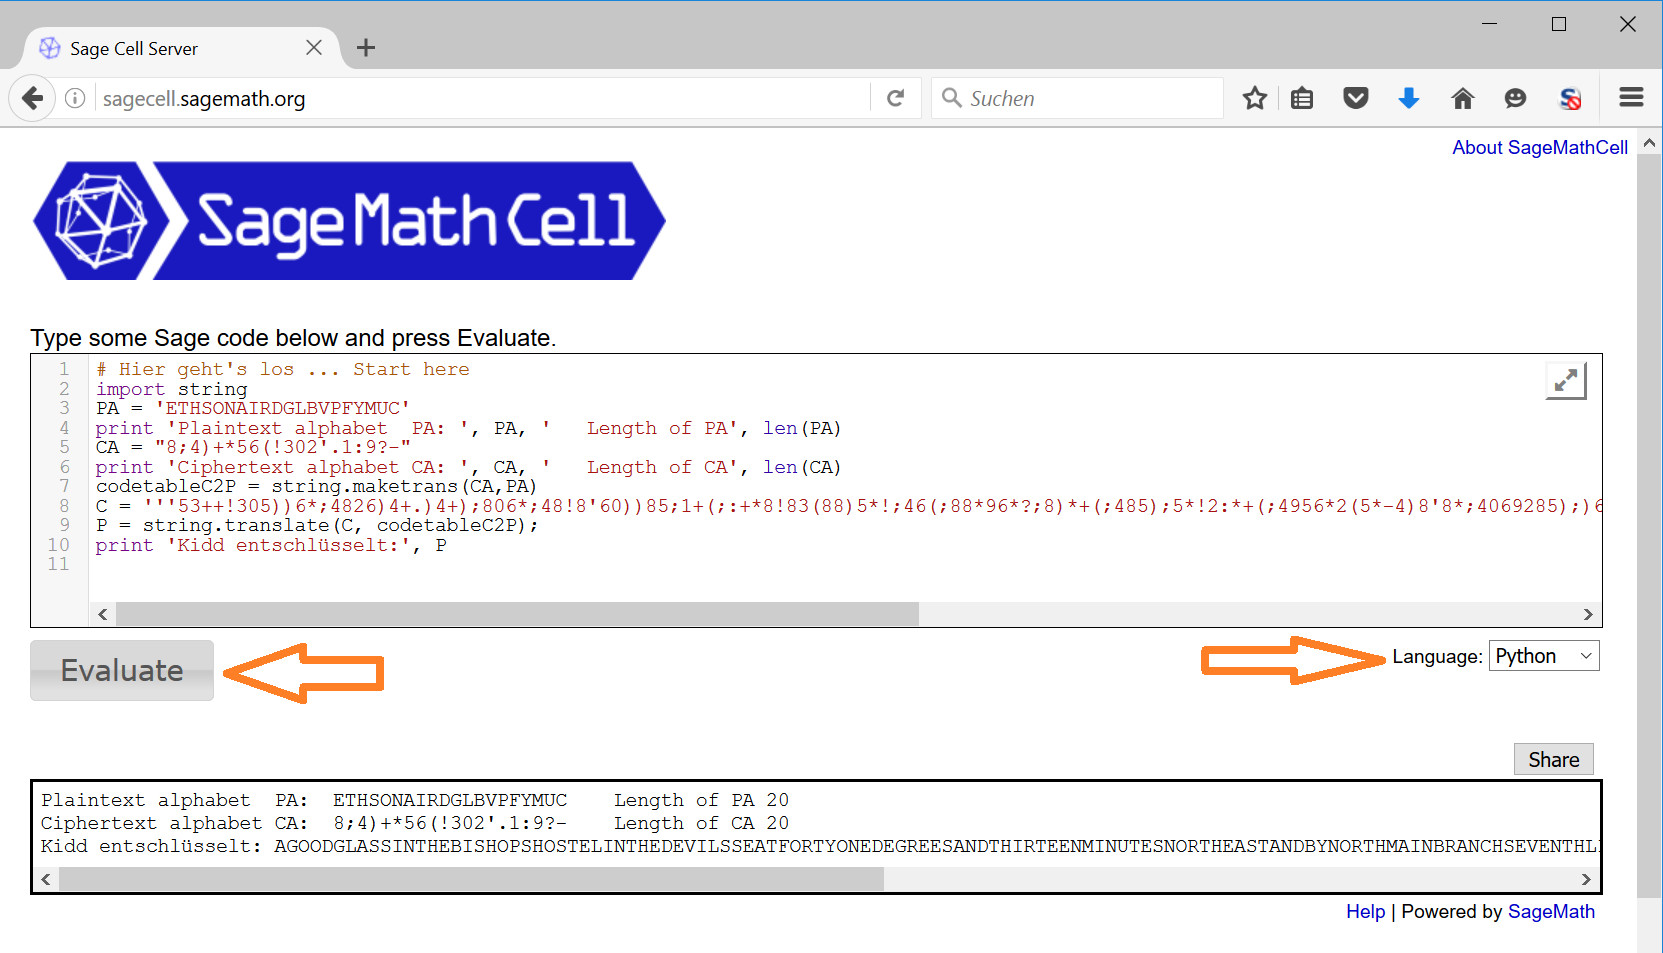
\includegraphics[scale=0.53]{../en/figures/Using-SageMathCell-with-Python-for-Poes-GoldBug}
\caption{Benutzung von SageMathCell, um Poes Goldk�fer zu entschl�sseln (mit Python\index{Python})}
\label{MOV_Using-SageMathCell-with-Python-for-Poes-GoldBug}
\end{center}
\end{figure}


\noindent Als Ergebnis erhalten wir:

% \noindent \verb muss auf derselben Zeile enden.
\begin{Verbatim}%

Plaintext alphabet  PA:  ETHSONAIRDGLBVPFYMUC    Length of PA 20
Ciphertext alphabet CA:  8;4)+*56(!302'.1:9?-    Length of CA 20
Kidd decrypted: AGOODGLASSINTHEBISHOPSHOSTELINTHEDEVILSSEATFORTYONEDEGREES
                ANDTHIRTEENMINUTESNORTHEASTANDBYNORTHMAINBRANCHSEVENTHLIMB
                EASTSIDESHOOTFROMTHELEFTEYEOFTHEDEATHSHEADABEELINEFROMTHE
                TREETHROUGHTHESHOTFIFTYFEETOUT

\end{Verbatim}

\noindent Man sieht gut, wie wenig Code man mit Python\index{Python} oder Sage f�r solche Aufgaben ben�tigt.
Im obigen Beispiel waren es 2 �berfl�ssige Kommentarzeilen, 3 Zeilen Eingabe, 3 Zeilen echter Code und 3 Zeilen Ausgabe;
effektiv n�tig waren 7 Zeilen Code.





% ++++++++++++++++++++++++++++++++++++++++++++++++++++++++++++++++++++++++++
\newpage
\hypertarget{appendix-Learn-NT}{}
\section{Lernprogramm Elementare Zahlentheorie}
    \label{s:appendix-Learn-NT}
    \index{ZT, Lernprogramm Zahlentheorie}%
    \index{Lernprogramm ZT}%

In CT1\index{CT1} ist ein interaktives Lernprogramm zur elementaren
{\em Zahlentheorie}, genannt "`ZT"', enthalten.\footnote{%
    ZT k�nnen Sie in CT1\index{CT1} �ber das Men�
    {\bf Einzelverfahren \textbackslash{} Zahlentheorie
    interaktiv \textbackslash{} Lernprogramm f�r Zahlentheorie} aufrufen.
}

Das Lernprogramm "`NT"' (Zahlentheorie) von Martin Ramberger f�hrt in die
Zahlentheorie ein und visualisiert viele der Verfahren und Konzepte.
Wo n�tig zeigt es auch die entsprechenden mathematischen Formeln.
Oftmals k�nnen die mathematischen Verfahren dynamisch mit eigenen kleinen
Zahlenbeispielen ausprobiert werden.

Die Inhalte basieren vor allem auf den B�chern von
\cite{Buchmann2016} und \cite{Scheid2006}.

Dieses visualisierte Lernprogramm wurde mit Authorware 4 erstellt.\footnote{%
    Da Authorware veraltet ist und der Hersteller keine Portierungswerkzeuge
    auf seine Nachfolgeprodukte zur Verf�gung stellte, wird das ZT-Programm
    nicht mehr weiter entwickelt.
}

\paragraph*{Bitte um Erweiterung/Upgrade:}
Ein Update auf die neueste Version von Authorware oder auf eine andere
Entwicklungsplattform w�re w�nschenswert. Wenn sich hierzu Interessenten
finden, w�rde ich mich sehr freuen (bitte E-Mail an den Autor des
CrypTool-Skriptes).


\paragraph*{Abbildungen:}
Die Abbildungen~\ref{NT_Fig_C1.3_EuclidsAlg-LinearCombinations}
bis~\ref{NT_Fig_C5.3_PollardRho} vermitteln einen Eindruck des
Lernprogramms "`ZT"':


% -> Figur 1  WIE ERREICHT MAN, dass er von vorne z�hlt ? (nicht wichtig)
%
% \includegraphics[scale=0.5]{figures/NT_Fig_C1.3_EuclidsAlg-LinearCombinations}
%    geht nicht. Im Dateinamen darf keine Punkt sein !!!?????!!!!!
%    Die Dateiendung muss man weglassen.
%
\begin{figure}[ht]
\begin{center}
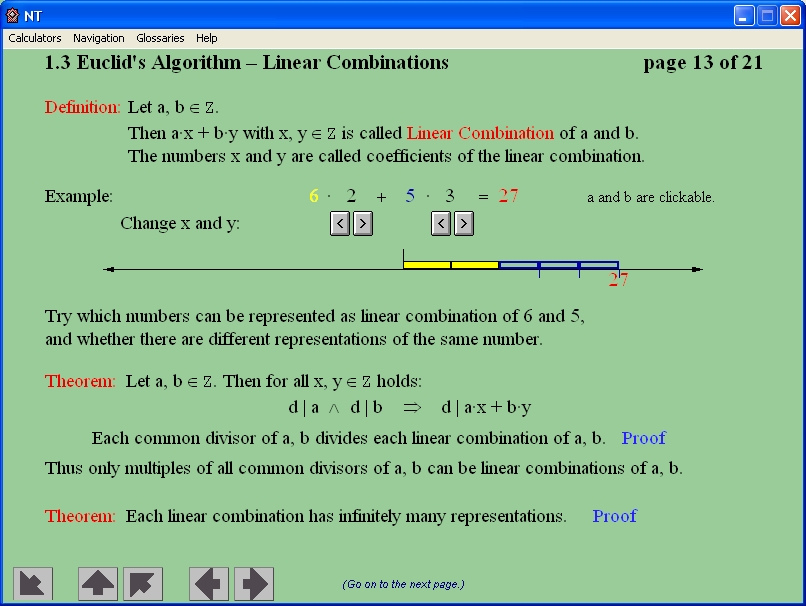
\includegraphics[scale=0.4]{figures/NT_Fig_C1-3_EuclidsAlg-LinearCombinations}
\caption{Jeder gemeinsame Teiler zweier Zahlen teilt auch alle ihre Linearkombinationen}
%%% TODO_Layout: Nur in Teilen von movies wird bei caption noch \vspace{1ex} hinzugef�gt.
%%%              Damit sind die Abst�nde im Abbildungsverzeichnis von A.9 bis A.16
%%%              unterschiedlich vom Rest --> nahm es wieder raus. Analog wurde etwas
%%%              Platz unter den Abb-Untertitel in Kap. 7 geschaffen, der nun auch weg (22.8.16)
%%%              --> Wenn man es macht, dann muss man es �berall machen!
%%% Bsp: vorher:  \caption{Euklids Algorithmus zur Bestimmung des ggT\vspace{1ex}}
%%%      nachher: \caption{Euklids Algorithmus zur Bestimmung des ggT}
\label{NT_Fig_C1.3_EuclidsAlg-LinearCombinations}
\end{center}
\end{figure}


\begin{figure}[ht]
\begin{center}
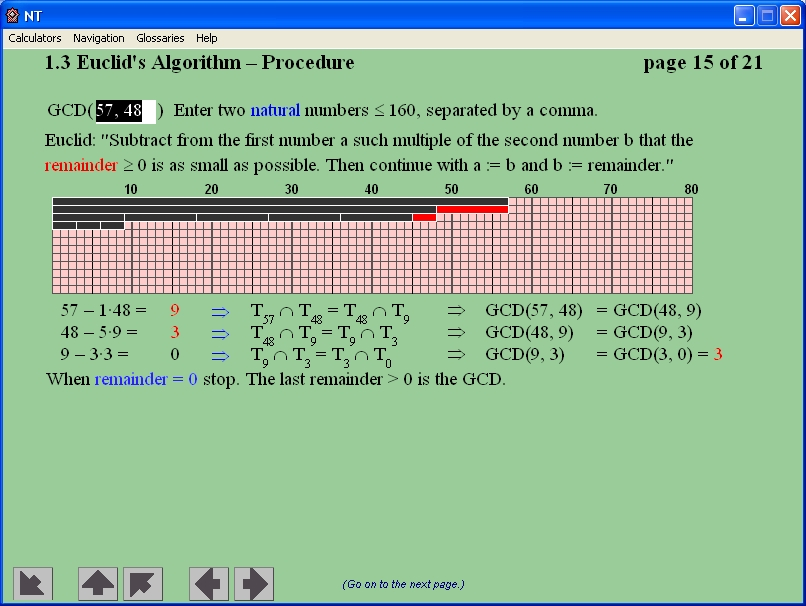
\includegraphics[scale=0.4]{figures/NT_Fig_C1-3_EuclidsAlg-Procedure}
\caption{Euklids Algorithmus zur Bestimmung des ggT}
\label{NT_Fig_C1.3_EuclidsAlg-Procedure}
\end{center}
\end{figure}


\begin{figure}[ht]
\begin{center}
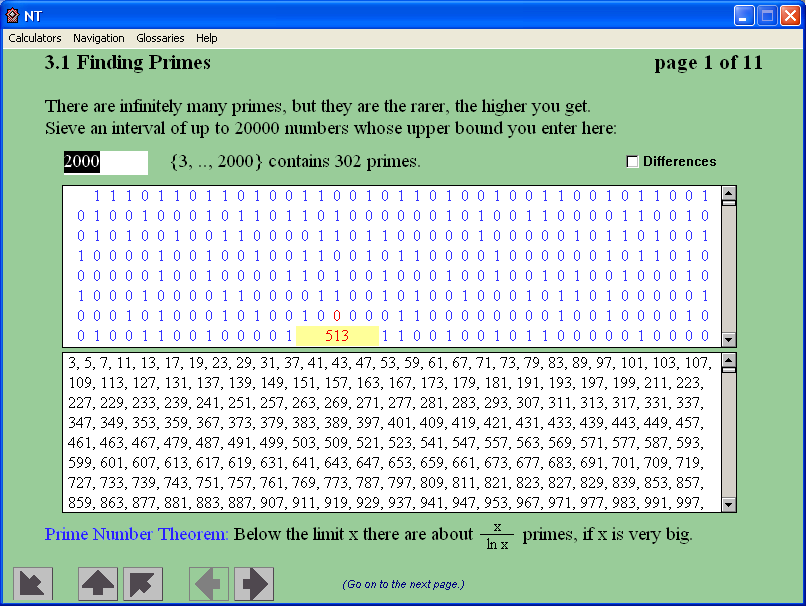
\includegraphics[scale=0.4]{figures/NT_Fig_C3-1_PrimesDistribution}
\caption{Verteilung der Primzahlen und ihrer Differenzen}
\label{NT_Fig_C3.1_PrimesDistribution}
\end{center}
\end{figure}


\begin{figure}[ht]
\begin{center}
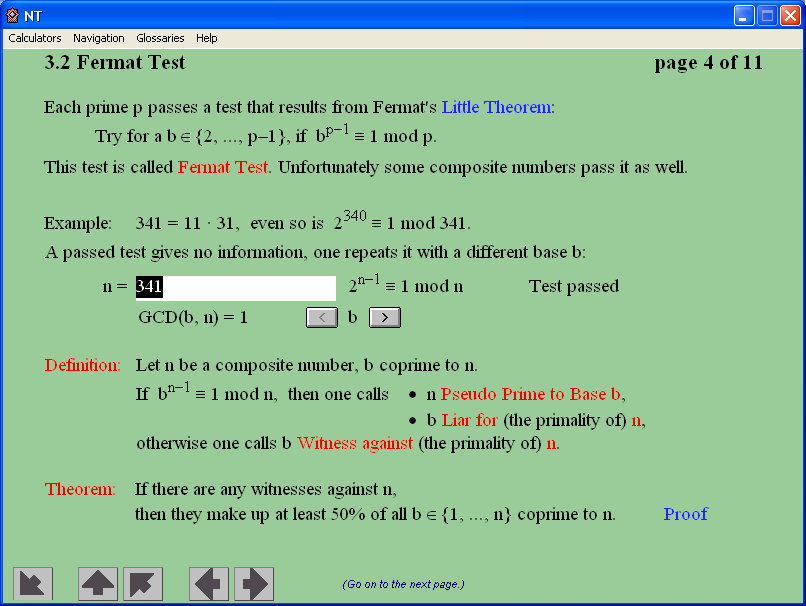
\includegraphics[scale=0.4]{figures/NT_Fig_C3-2_Fermat-Test}
\caption{Primzahlen finden mit dem Primzahltest nach Fermat}
\label{NT_Fig_C3.2_Fermat-Test}
\end{center}
\end{figure}


\begin{figure}[ht]
\begin{center}
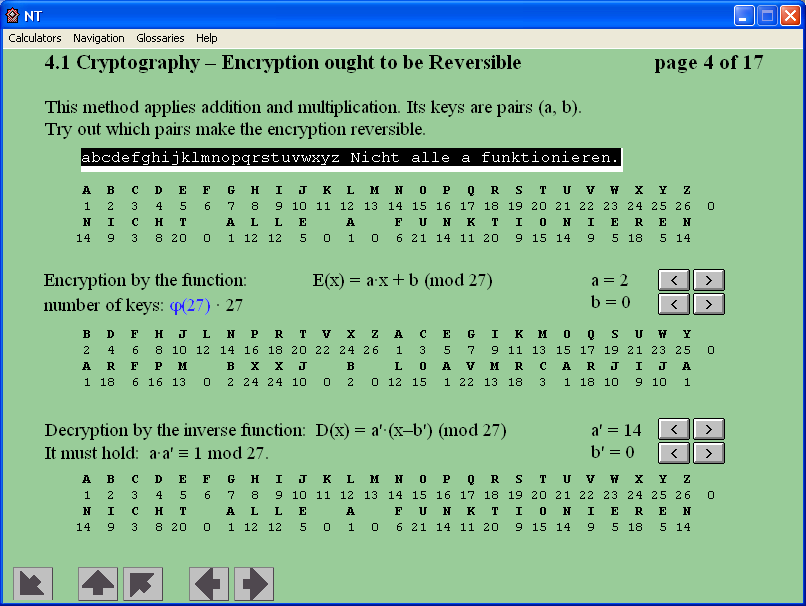
\includegraphics[scale=0.4]{figures/NT_Fig_C4-1_ReversibilityAdditiveCipher}
\caption{Umkehrbarkeit von Verschl�sselungsalgoritmen am Beispiel additiver Chiffren}
\label{NT_Fig_C4.1_ReversibilityAdditiveCipher}
\end{center}
\end{figure}


\begin{figure}[ht]
\begin{center}
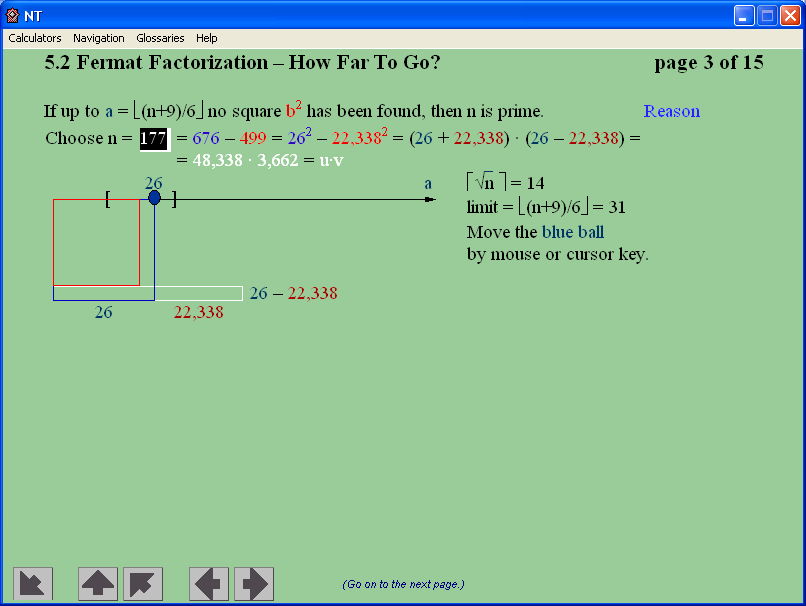
\includegraphics[scale=0.4]{figures/NT_Fig_C5-2_Fermat-factorization-How-far-1}
\caption{Fermat-Faktorisierung m.H. der 3. Binomischen Formel}
\label{NT_Fig_C5.2_Fermat-factorization-How-far-1}
\end{center}
\end{figure}


\begin{figure}[ht]
\begin{center}
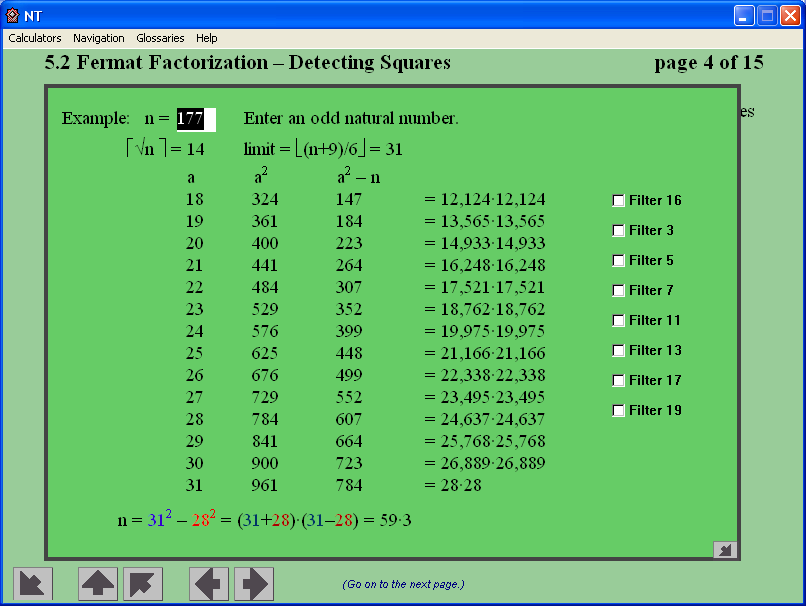
\includegraphics[scale=0.4]{figures/NT_Fig_C5-2_Fermat-factorization-How-far-2}
\caption{Fermat-Faktorisierung: Quadrate erkennen}
\label{NT_Fig_C5.2_Fermat-factorization-How-far-2}
\end{center}
\end{figure}


\begin{figure}[ht]
\begin{center}
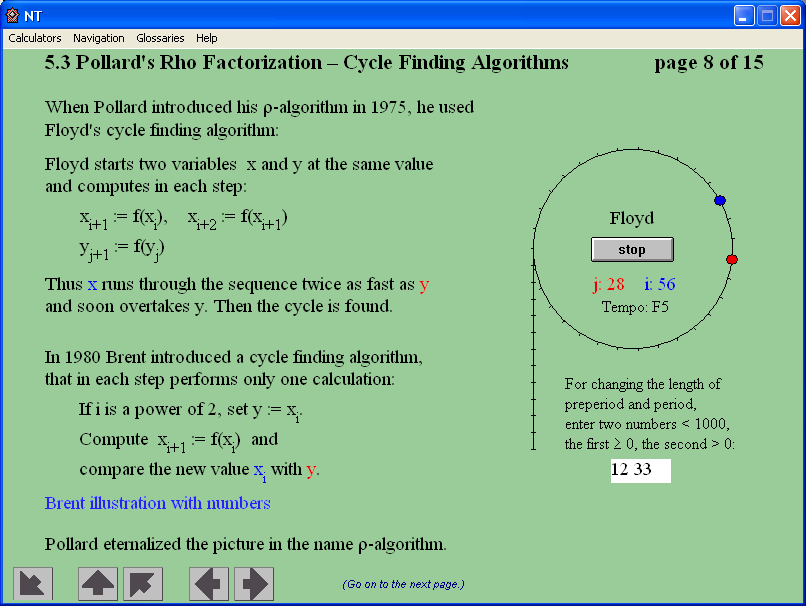
\includegraphics[scale=0.4]{figures/NT_Fig_C5-3_PollardRho}
\caption{Pollards Rho-Faktorisierung: Kreisfindungsalgorithmus nach Floyd}
\label{NT_Fig_C5.3_PollardRho}
\end{center}
\end{figure}



%------------------------------------------------------------------------------
% \clearpage   % N�tig, damit Lit.verzeichnis nicht gl. nach Abb. 8 kommt.
% \newpage
\putbib[../de/references]
\addcontentsline{toc}{section}{Literaturverzeichnis}
\end{bibunit}



  \renewcommand{\CTBChapName}{(Appendix Sage)}       % $Id:
% !Mode:: "TeX:DE"    % Setting document mode and submode for WinEdt
% ..............................................................................
%             W A S  I S T  S A G E M A T H  ?
% ~~~~~~~~~~~~~~~~~~~~~~~~~~~~~~~~~~~~~~~~~~~~~~~~~~~~~~~~~~~~~~~~~~~~~~~~~~~~~~

\newpage
\hypertarget{appendix-using-sage}{}
\section{Kurzeinf�hrung in das CAS SageMath}
\label{s:appendix-using-sage}
\index{SageMath}
\index{SageMath!Programmbeispiele}

%% Unter \url{https://wiki.sagemath.org/combinat} gibt es Weiterentwicklung on-top of Sage.
%% Diese kommen meist nach und nach ins offizielle Sage rein.


Dieses Buch enth�lt zahlreiche mit SageMath erstellte Programmbeispiele. SageMath ist
ein Open-Source Computer-Algebra-System (CAS), das f�r Lehre, Studium und Forschung
eingesetzt wird.
SageMath kombiniert viele hochwertige Open-Source-Packete\footnote{%
Einen Eindruck von der Gr��e von SageMath erh�lt man, wenn man es selbst compiliert:
Die heruntergeladenen Sourcen von SageMath 4.1 brauchten zur Compilierung auf einem
durchschnittlichen Linux-PC rund 5 h (inklusive aller Bibliotheken).
Danach nahm es 1,8 GB Plattenplatz ein.
}
und liefert den Zugang zu deren Funktionalit�t �ber ein gemeinsames, auf der
Programmiersprache Python\index{Python} basierendes Interface\footnote{%
Es gibt auch ein relativ einfaches Interface f�r die Sprache C, genannt Cython,
mit der man eigene Funktionen in SageMath stark beschleunigen kann.\\
Siehe \url{http://openwetware.org/wiki/Open_writing_projects/Sage_and_cython_a_brief_introduction}.
}.

\noindent SageMath kann man auf vielf�ltige Weise nutzen:
als m�chtigen Taschenrechner; als Tool f�r das Mathematikstudium;
oder als Programmier-Umgebung, um Algorithmen zu prototypen oder um Forschung im
Bereich der algorithmischen Aspekte der Mathematik zu betreiben.

\noindent Einen schnellen Einstieg bieten z.B. die Referenzen in dieser Fu�note%
\footnote{%
\noindent\hangindent=6pt\makebox[6pt][l]{-}\glqq Einladung zu Sage\grqq~von David Joyner, letztes Update 2009,\\
  \url{http://sage.math.washington.edu/home/wdj/teaching/calc1-sage/an-invitation-to-sage.pdf}

\noindent\hangindent=6pt\makebox[6pt][l]{-}\glqq The SDSU Sage Tutorial\grqq,\\
  \url{http://www-rohan.sdsu.edu/~mosulliv/sagetutorial/}\\
  \url{http://www-rohan.sdsu.edu/~mosulliv/sagetutorial/sagecalc.html}

  \noindent\hangindent=6pt\makebox[6pt][l]{-}{\glqq SAGE For Newbies\grqq~von Ted Kosan, 2007,\\
  \url{http://sage.math.washington.edu/home/tkosan/newbies_book/sage_for_newbies_v1.23.pdf}}
   % Leerzeile am Ende n�tig, sonst hat die letzte Zeile KEINEN h�ngenden Einzug?! (TODO_LaTeX)
   %%%% Aber das auch unsch�n.
}.

\noindent Die offizielle SageMath Online-Dokumentation\footnote{%
  Die entsprechenden offiziellen PDF-Dokuments k�nnen herunter geladen werden von\\
  \url{http://www.sagemath.org/help.html}, \url{http://www.sagemath.org/doc} und \url{http://planet.sagemath.org}.
} finden Sie unter: \url{http://www.sagemath.org}.


\noindent Es gibt inzwischen viele PDF- und HTML-Dokumente �ber SageMath, so dass wir als guten Startpunkt nur einige wenige nennen\footnote{%
- \glqq Bibliothek\grqq: {\centering \url{http://www.sagemath.org/library.html}},\\
- \glqq Dokumentationsprojekt\grqq:
  {\centering \url{http://wiki.sagemath.org/DocumentationProject}},\\
- \glqq Lehrmaterial\grqq: {\centering \url{http://wiki.sagemath.org/Teaching_with_SAGE}}.
}.

\noindent Auch beim Studium der Kryptologie k�nnen fertige SageMath-Module genutzt
werden\footnote{%
\noindent\hangindent=6pt\makebox[6pt][l]{-}�berblick,
   welche Kryptographie momentan in SageMath enthalten ist:\\
   \url{http://www.sagemath.org/doc/reference/sage/crypto/}

\noindent\hangindent=6pt\makebox[6pt][l]{-}Diskussionen
   �ber Lernaspekte beim Entwickeln weiterer Krypto-Module in SageMath:\\
   \url{http://groups.google.com/group/sage-devel/browse_thread/thread/c5572c4d8d42d081}
% Leerzeile bei den Aufz�hlungen am Ende n�tig, damit die 2. Zeile (Url) h�ngenden Einzug hat.
% ABER: Bei der letzten Aufz�hlung f�hrt Leerzeile zu leerer Zeile (was nicht gewollt ist) und die letzte Url hat trotzdem keinen h�ngenden Einzug! (TODOTODO)
}.

\noindent Umfangreiche Kryptographie-Einf�hrungen finden sich in der folgenden Fu�note\footnote{%
\noindent\hangindent=6pt\makebox[6pt][l]{-}Ein fertiger Kryptographie-Kurs von David Kohel,
  der SageMath nutzt, aus 2008:\\
  {\centering \url{http://www.sagemath.org/files/kohel-book-2008.pdf} }\\
  bzw. derselbe Kurs in einer neueren Fassung (2015)\\
  {\centering \url{http://iml.univ-mrs.fr/~kohel/tch/M2-CryptoSymetrique/crypto.pdf} }.

\noindent\hangindent=6pt\makebox[6pt][l]{-}\glqq Introduction to Cryptography with
  Open-Source Software\grqq, ein hervorragendes Buch von Alasdair McAndrew, CRC, 2011
  %% TODO: Wenn die eine Zeile l�nger, beginnt sie doch wieder ganz vorne!
}.


% ---------------------------------------------------------------------------
\section*{SageMath-Benutzerschnittstellen}
SageMath ist kostenlos und kann von folgender Webseite herunter geladen werden:
\begin{center}
  \url{http://www.sagemath.org} \\
\end{center}
Standardm��ig nutzt man die SageMath-{\bf Kommandozeile} als Interface, wie im
folgenden Bild~\ref{fig:sage_cmd_interfaces} zu sehen ist.
Es gibt jedoch auch ein grafisches Benutzerinterface f�r diese Software
in Form des SageMath-Notebooks (siehe Bild~\ref{fig:sage_gui_interfaces}).
Und schlie�lich kann man SageMath-{\bf Notebooks}\footnote{%
Weitere Details zu SageMath-Notebooks finden Sie in
Kapitel~\ref{ec:Sage_Massierer}
(\glqq \nameref{ec:Implementing-for-Education}\grqq
  $\Rightarrow$ \glqq \nameref{ec:Sage_Massierer}\grqq).
                      }
auch online auf verschiedenen Servern nutzen, ohne SageMath lokal zu installieren, z.B.:
\begin{center}
\url{http://sagecell.sagemath.org/} oder \\
\url{https://cocalc.com/}
\end{center}

SageMath l�uft unter den Betriebssystemen Linux, Mac OS X und Windows.
Auf der Windows-Plattform l�uft die komplette SageMath-Distribution momentan
nur als ein VMware-Image.

\begin{figure}[!htpb]
\centering
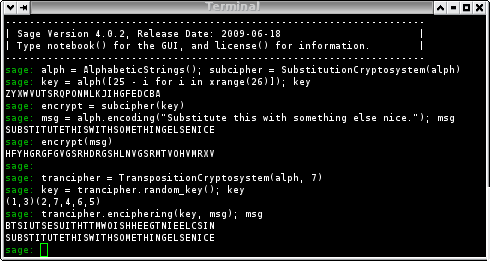
\includegraphics[scale=0.6]{figures/sage-cmd}
\caption{SageMath-Kommandozeilen-Interface}
\label{fig:sage_cmd_interfaces}
\end{figure}

\begin{figure}[!htpb]
\centering
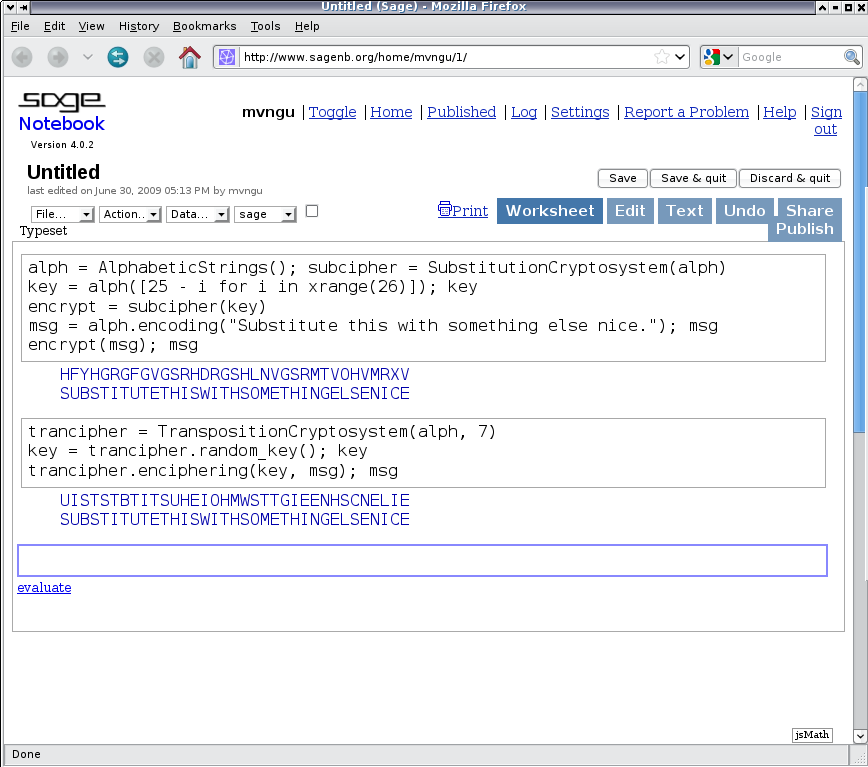
\includegraphics[scale=0.4]{figures/sage-gui}
\caption[SageMath-Notebook-Interface]{SageMath-Notebook-Interface\footnotemark}
\label{fig:sage_gui_interfaces}
\end{figure}

\footnotetext{%
Um das grafische SageMath-Interface lokal zu starten, muss man auf der SageMath-Kommandozeile
\verb#notebook()# eingeben. Danach startet der eingestellte Browser (Iceweasel,
Firefox, IE, ...) z.B. mit der URL \textit{http://localhost:8000}.
}



% ---------------------------------------------------------------------------
\newpage
\section*{Hilfe beim Benutzen von SageMath}

Wenn man SageMath auf der Kommandozeile startet, erh�lt etwas wie die folgenden Zeilen:
%
\begin{Verbatim}%
[fontsize=\footnotesize]
mnemonic:~$ sage
----------------------------------------------------------------------
| Sage Version 4.1, Release Date: 2009-07-09                         |
| Type notebook() for the GUI, and license() for information.        |
----------------------------------------------------------------------

sage: help
Type help() for interactive help, or help(object) for help about object.
sage:
sage:
sage: help()

Welcome to Python 2.6!  This is the online help utility.

If this is your first time using Python, you should definitely check out
the tutorial on the Internet at http://docs.python.org/tutorial/.

Enter the name of any module, keyword, or topic to get help on writing
Python programs and using Python modules.  To quit this help utility and
return to the interpreter, just type "quit".

To get a list of available modules, keywords, or topics, type "modules",
"keywords", or "topics".  Each module also comes with a one-line summary
of what it does; to list the modules whose summaries contain a given word
such as "spam", type "modules spam".
\end{Verbatim}
%
Viele weitere Hilfen gibt es als offizielle SageMath-Dokumentation, die mit jedem
Release von SageMath verteilt wird~(siehe Bild~\ref{fig:sage_standard_doc}).
%
\begin{figure}[!htpb]
\centering
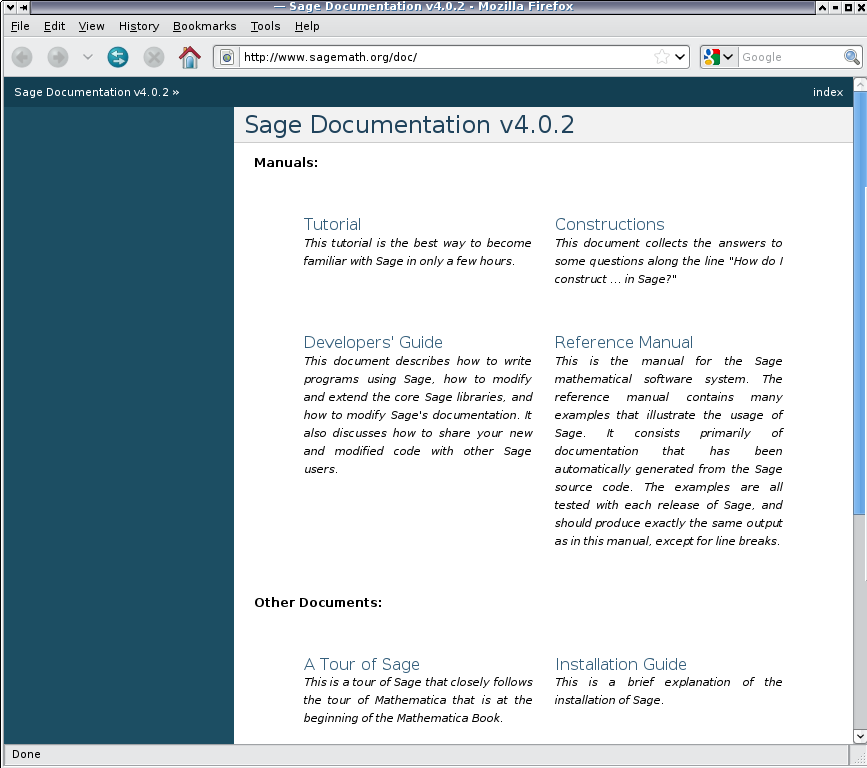
\includegraphics[scale=0.4]{figures/sage-online-doc}
\caption{Die Standard-Dokumentation von SageMath}
\label{fig:sage_standard_doc}
\end{figure}
%
Zur offiziellen SageMath-Standard-Dokumentation geh�ren folgende Dokumente:

\begin{itemize}
\item Tutorial --- Das Tutorial ist f�r SageMath-Einsteiger.
  Es ist daf�r gedacht, sich in ein bis drei Stunden mit den
  wichtigsten Funktionen vertraut zu machen.

\item Constructions --- Dieses Dokument ist im Stil eines \glqq Kochbuchs\grqq~mit
  einer Sammlung von Antworten auf Fragen zur Konstruktion von SageMath-Objekten.

\item Developers' Guide --- Dieser F�hrer ist f�r Entwickler, die selbst SageMath
  mit weiter entwickeln wollen. Enthalten sind darin z.B. Hinweise zum
  Stil und zu Konventionen beim Programmieren, zur Modifikation von
  SageMath-Kern-Bibliotheken oder von SageMath-Standard-Dokumentation, und zum Code-Review
  und zur Software-Verteilung.

\item Reference Manual --- Dieses Handbuch enth�lt die komplette Dokumentation
  aller wichtigen SageMath-Funktionen. Zu jeder Klassen-Beschreibung gibt es
  mehrere Code-Beispiele. Alle Code-Beispiele im Referenz-Handbuch werden
  bei jedem neuen SageMath-Release getestet.

\item Installation Guide --- Dieser F�hrer erkl�rt, wie man SageMath auf
  verschiedenen Plattformen installiert.

\item A Tour of Sage --- Diese Tour durch SageMath zeigt exemplarisch verschiedene
  Funktionen, die f�r Einsteiger sinnvoll sind.

\item Numerical Sage --- Dieses Dokument f�hrt Werkzeuge auf, die in SageMath
  f�r numerische Mathematik verf�gbar sind.

\item Three Lectures about Explicit Methods in Number Theory Using
  Sage --- Drei Vorlesungen �ber Methoden der Zahlentheorie, die explizit
  SageMath nutzen. Dieses Dokument zeigt wie man mit SageMath Berechnungen in
  fortgeschrittener Zahlentheorie durchf�hrt.
\end{itemize}

\noindent Von der SageMath-Kommandozeile erh�lt man eine Liste aller verf�gbaren Kommandos
(Funktionsnamen etc.), die ein bestimmtes Muster haben, wenn man die ersten Zeichen tippt,
und dann die \glqq Tab\grqq-Taste dr�ckt:
%
\begin{Verbatim}%
[fontsize=\footnotesize]
sage: Su[TAB]
Subsets                   Subwords                  SuzukiGroup
SubstitutionCryptosystem  SupersingularModule
\end{Verbatim}
%
Wenn man den genauen Namen eines Kommandos kennt, kann man die \texttt{help}-Funktion
nutzen oder das Fragezeichen \glqq ?\grqq~anf�gen, um weitere Informationen zu
diesem Kommando zu erhalten.  Zum Beispiel liefert das Kommando
\texttt{help(SubstitutionCryptosystem)} die Dokumentation zur der eingebauten
Klasse \texttt{SubstitutionCryptosystem}. Mit dem Fragezeichen erhalten wir die
Dokumentation zu dieser Klasse auf folgende Weise:
%
\begin{Verbatim}%
[fontsize=\footnotesize]
sage: SubstitutionCryptosystem?
Type:type
Base Class:<type 'type'>
String Form:<class 'sage.crypto.classical.SubstitutionCryptosystem'>
Namespace:Interactive
File:/home/mvngu/usr/bin/sage-3.4.1/local/lib/python2.5/site-packages/sage/crypto/classical.py
Docstring:

        Create a substitution cryptosystem.

        INPUT:

        - ``S`` - a string monoid over some alphabet

        OUTPUT:

        - A substitution cryptosystem over the alphabet ``S``.

        EXAMPLES::

            sage: M = AlphabeticStrings()
            sage: E = SubstitutionCryptosystem(M)
            sage: E
            Substitution cryptosystem on Free alphabetic string monoid
            on A-Z
            sage: K = M([ 25-i for i in range(26) ])
            sage: K
            ZYXWVUTSRQPONMLKJIHGFEDCBA
            sage: e = E(K)
            sage: m = M(``THECATINTHEHAT'')
            sage: e(m)
            GSVXZGRMGSVSZG

        TESTS::

            sage: M = AlphabeticStrings()
            sage: E = SubstitutionCryptosystem(M)
            sage: E == loads(dumps(E))
            True
\end{Verbatim}
%
\vspace{30pt}
Weitere Unterst�tzung f�r spezifische Probleme gibt es in den Archiven der
\texttt{sage-support} Mailing-Liste unter
%
\begin{center}
  \url{http://groups.google.com/group/sage-support}
\end{center}




% ---------------------------------------------------------------------------
\newpage
\section*{Beispiele f�r in SageMath eingebaute mathematische Funktionen}

Hier sind ein paar kleine Beispiele\footnote{%
Diese Beispiele stammen aus dem Blog von Dr. Alasdair McAndrew, Victoria University,\\
\url{http://amca01.wordpress.com/2008/12/19/sage-an-open-source-mathematics-software-system}}
(alle f�r das Kommandozeilen-Interface -- zur einfacheren Nutzung), um zu sehen,
was man mit SageMath machen kann:

\begin{sagecode}
\begin{Verbatim}%
[fontsize=\footnotesize]
# * Analysis (Infinitesimalrechnung):
    sage: x=var('x')
    sage: p=diff(exp(x^2),x,10)*exp(-x^2)
    sage: p.simplify_exp()
     1024 x^10 + 23040 x^8 + 161280 x^6 + 403200 x^4 + 302400 x^2 + 30240

# * Lineare Algebra:
    sage: M=matrix([[1,2,3],[4,5,6],[7,8,10]])
    sage: c=random_matrix(ZZ,3,1);c
     [ 7 ]
     [-2 ]
     [-2 ]
    sage: b=M*c
    sage: M^-1*b
     [ 7 ]
     [-2 ]
     [-2 ]

# * Zahlentheorie:
    sage: p=next_prime(randint(2^49,2^50));p
      1022095718672689
    sage: r=primitive_root(p);r
      7
    sage: pl=log(mod(10^15,p),r);pl
      1004868498084144
    sage: mod(r,p)^pl
      1000000000000000

# * Endliche K�rper (\url{http://de.wikipedia.org/wiki/Endlicher_K%C3%B6rper}):
    sage: F.<x>=GF(2)[]
    sage: G.<a>=GF(2^4,name='a',modulus=x^4+x+1)
    sage: a^2/(a^2+1)
      a^3 + a
    sage: a^100
      a^2 + a + 1
    sage: log(a^2,a^3+1)
      13
    sage: (a^3+1)^13
      a^2
\end{Verbatim}
\caption{Einige kleine Beispiele in SageMath aus verschiedenen Gebieten der Mathematik}
\end{sagecode}



% ---------------------------------------------------------------------------
\newpage
\section*{Programmieren mit SageMath}

Wenn man ein CAS (Computer-Algebra-System) nutzt, schreibt man zu Beginn einzelne
Befehle in die Kommandozeile wie im obigen Beispiel\footnote{%
  Standardm��ig wird SageMath-Code auch so pr�sentiert: Dabei beginnen die Zeilen
  mit  \glqq sage:\grqq~und \glqq ...\grqq.
  \begin{Verbatim}%
  [fontsize=\footnotesize]
  sage: m = 11
  sage: for a in xrange(1, m):
  ....:     print [power_mod(a, i, m) for i in xrange(1, m)]
  ....:
  \end{Verbatim}

  \noindent Auch dieses Skript benutzt normalerweise die obige Konvention, um
  SageMath-Code zu pr�sentieren, solange der Code nicht aus einer SageMath-Skriptdatei kommt.
  Wenn man den SageMath-Code aus diesem Skript kopiert und per Paste auf der SageMath-Kommandozeile
  wieder einf�gt, sollte man \glqq sage:\grqq~und \glqq ...\grqq~ weglassen
  (obwohl das Kommandozeilen-Interface in den meisten F�llen mit diesen Pr�fixen
  korrekt umgehen kann).}.

Wenn man eigene Funktionen entwickelt, sie �ndert und aufruft, dann ist es viel einfacher,
die Entwicklung in einem eigenen Editor vorzunehmen, den Code als SageMath-Skriptdatei zu
speichern und die Funktionen nicht-interaktiv auf der Kommandozeile auszuf�hren.
Beide Arten, Code zu entwickeln, wurden in
Kapitel \ref{CM_Sage_samples} (\glqq \nameref{CM_Sage_samples}\grqq),
Kapitel \ref{PaP_Sage_samples} (\glqq \nameref{PaP_Sage_samples}\grqq),
Kapitel \ref{primes:_Appendix_Sage-Samples} (\glqq \nameref{primes:_Appendix_Sage-Samples}\grqq)
und in Kapitel \ref{NumberTheory_Appendix_E} (\glqq\nameref{NumberTheory_Appendix_E}\grqq)
angewandt.

\noindent Um SageMath-Code in einem eigenen Editor zu entwickeln und zu testen, gibt es zwei
n�tzliche Befehle: \verb!load()! und \verb!attach()!\footnote{%
Vergleiche das SageMath-Tutorial �ber Programmierung, Kapitel
\glqq Loading and Attaching Sage files\grqq,\\
\url{http://doc.sagemath.org/html/en/tutorial/programming.html}.}.\\
Angenommen Sie haben die folgende Funktions-Definition:
\begin{Verbatim}%
   [fontsize=\footnotesize]
   def function(var1):
       r"""
       DocText.
       """
       ...
       return (L)
\end{Verbatim}
\noindent die in der Datei \texttt{primroots.sage} gespeichert wurde.

\noindent Um diese Funktion in SageMath zu laden (und syntaktisch gleich zu testen),
wird der Befehl \verb!load()! benutzt:

\texttt{sage: load primroots.sage}

\noindent Danach kann man auf der Kommandozeile alle Variablen und Funktionen
nutzen, die im Sage\-Math-Skript definiert wurden\footnote{%
Anmerkungen:

\noindent\hangindent=6pt\makebox[6pt][l]{-}Bitte keine Leerzeichen
oder White Spaces im Dateinamen.

\noindent\hangindent=6pt\makebox[6pt][l]{-}Es empfiehlt sich,
der SageMath-Skriptdatei die Datei-Extension
\glqq .sage\grqq~statt \glqq .py\grqq~zu geben.
Hat ein SageMath-Skript die Dateinamens-Endung \glqq .sage\grqq, dann wird
beim Laden der Datei in SageMath auch gleich die normale SageMath-Umgebung mit geladen,
um die Syntax zu pr�fen. Genauso funktioniert es, wenn man ein SageMath-Skript direkt
von einer Bash-Shell aufruft mit~~\texttt{\$ sage primroots.sage}.

\noindent\hangindent=6pt\makebox[6pt][l]{-}Beim Laden des obigen
SageMath-Skripts wird es von SageMath zuerst geparst, und dann
in eine andere Datei namens \glqq primroots.py\grqq~kopiert. SageMath erg�nzt
dann alle notwendigen Variablen in \glqq primroots.py\grqq~und alle Import-Statements.
Somit wird das SageMath-Skript genauso ausgef�hrt, als h�tte man die Befehle einzeln
auf der Kommandozeile eingetippt. Ein bedeutender Unterschied ist,
dass alle Ausgaben ein \verb!print!~ben�tigen.

}.

Normalerweise editiert man ein eigenes SageMath-Skript wieder und m�chte dann den
Inhalt des ge�nderten Skripts wieder in SageMath laden. Daf�r kann man den Befehl
\verb!attach()! nutzen (man kann auch direkt nach dem \verb!load()!
das \verb!attach()! aufrufen, und nicht erst, wenn man das Skript �ndert;
man kann \verb!load()! sogar weglassen, da dies in \verb!attach()! enthalten ist):

\texttt{sage: attach primroots.sage}

Nun kann man das SageMath-Skript �ndern und die ge�nderte Funktionsdefinition
wird -- solange man die SageMath-Session nicht beendet -- beim n�chsten Enter
in SageMath geladen (und syntaktisch gleich gepr�ft). Diese Neuladen passiert
vollkommen automatisch. Der Befehl attach() l�sst SageMath also permanent die
genannte Datei auf �nderungen �berwachen. Damit spart man sich das Kopieren
und Pasten zwischen dem eigenen Texteditor und dem SageMath-Kommandozeilen-Interface.

Hier ist ein Bild, das SageMath-Code im Editor GVIM zeigt -- mit aktiviertem
Syntax-Highlighting (siehe Bild~\ref{fig:sage-highlighted-code-in-editor}).
%
\begin{figure}[!htpb]
\centering
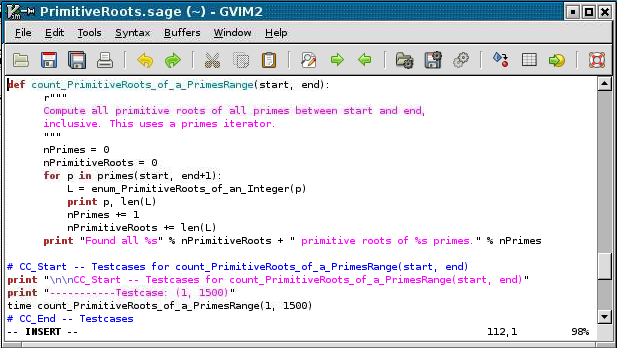
\includegraphics[scale=0.7]{figures/sage-highlighted-code-in-editor}
\caption{SageMath-Beispiel in einem Editor mit aktiviertem Code-Highlighting}
\label{fig:sage-highlighted-code-in-editor}
\end{figure}

\vspace{20pt}
Falls man die Ausgabe einer attachten Datei so angezeigt haben m�chte,
wie wenn man die Einzelbefehle direkt auf der Kommandozeile eingibt
(also nicht nur das, was per \verb!print! ausgegeben wird),
kann man den Befehl \verb!iload()! verwenden:
Jede Zeile wird dann einzeln geladen. Um die n�chste Zeile zu laden,
muss man die \verb!Enter!-Taste dr�cken. Das muss man so lange wiederholen,
bis alle Zeilen des SageMath-Skripts in die SageMath-Session geladen sind.

\texttt{sage: iload primroots.sage}


% \vspace{30pt}
\newpage
\noindent Weitere Hinweise:
\begin{itemize}
  \item Abfrage der Version Ihrer SageMath-Umgebung mit: \texttt{version()}
  \item Um sich schnell die SageMath-Programmbeispiele in diesem Skript anzusehen, k�nnen Sie
    \begin{itemize}
      \item im Index nach \verb#SageMath -> Programmbeispiele# schauen, oder
      \item sich im Anhang das \glqq \nameref{sc:List-of-Sage-Code-Examples}\grqq~ansehen.
    \end{itemize}
  \item Die SageMath-Beispiele in diesem Skript werden mit CrypTool ausgeliefert.\\
        Weitere Details am Ende der �bersicht
        \glqq \nameref{sc:List-of-Sage-Code-Examples}\grqq.
\end{itemize}



  \renewcommand{\CTBChapName}{(Appendix Authors)}    \section{Autoren dieses Skripts}
\hypertarget{appendix-authors}{}\label{s:appendix-authors}

Dieser Anhang f"uhrt die Autoren des CrypTool-Skripts auf. Am Anfang jedes
Kapitels werden die Autoren angegeben, die zu diesem Kapitel beigetragen haben.

\begin{description}
\item[Bernhard Esslinger,] Initiator von CrypTool, Leiter IT Security in der Deutschen
Bank und Dozent an der Universit"at Siegen.
 
\item[Matthias B"uger,] Mitautor des Kapitels ``Elliptische Kurven'',
Research Analyst bei der Deutschen Bank, verantwortlich f"ur den Deutsche Bank
Kryptographie-Standard.

\item[Bartol Filipovic,] urspr"unglicher Autor der
Elliptische-Kurven-Implementierung in CrypTool und des entsprechenden Kapitels
in diesem Skript.

\item[Henrik Koy, ] Hauptentwickler und Koordinator der CrypTool-Entwicklung
seit Version 1.3, Reviewer des Skripts und \TeX{}-Guru, Projektleiter IT bei der
Deutschen Bank.

\item[Roger Oyono, ] Implementierer des Faktorisierungs-Dialogs in CrypTool und urspr"unglicher Autor des Kapitels "`Die mathematischen Ideen hinter der modernen Kryptographie"'.

\item[J"org Cornelius Schneider,] Design und Support von CrypTool,
Kryptographie-Enthusiast und Projektleiter IT bei der Deutschen Bank.

\end{description}


\end{appendix}

\renewcommand{\CTBChapName}{(Appendix gnu-fdl)}      % This is set up to run with pdflatex.
%---------The file header---------------------------------------------
% \documentclass[a4paper,12pt]{book}

% \usepackage[english]{babel} %language selection
% \selectlanguage{english}

% \pagenumbering{arabic}

% \usepackage{hyperref}
% \hypersetup{colorlinks,
%            citecolor=black,
%            filecolor=black,
%            linkcolor=black,
%            urlcolor=black,
%            bookmarksopen=true,
%            pdftex}

% \hfuzz = .6pt % avoid black boxes

% \begin{document}
%---------------------------------------------------------------------
\chapter*{\rlap{GNU Free Documentation License}}
% \phantomsection  % so hyperref creates bookmarks
\addcontentsline{toc}{chapter}{GNU Free Documentation License}
%\label{label_fdl}

\begin{center}

       Version 1.3, 3 November 2008


 Copyright \copyright{} 2000, 2001, 2002, 2007, 2008  Free Software Foundation, Inc.

 \bigskip

     \url{http://fsf.org/}

 \bigskip

 Everyone is permitted to copy and distribute verbatim copies
 of this license document, but changing it is not allowed.
\end{center}


\begin{center}
{\bf\large Preamble}
\end{center}

The purpose of this License is to make a manual, textbook, or other
functional and useful document ``free'' in the sense of freedom: to
assure everyone the effective freedom to copy and redistribute it,
with or without modifying it, either commercially or noncommercially.
Secondarily, this License preserves for the author and publisher a way
to get credit for their work, while not being considered responsible
for modifications made by others.

This License is a kind of ``copyleft'', which means that derivative
works of the document must themselves be free in the same sense.  It
complements the GNU General Public License, which is a copyleft
license designed for free software.

We have designed this License in order to use it for manuals for free
software, because free software needs free documentation: a free
program should come with manuals providing the same freedoms that the
software does.  But this License is not limited to software manuals;
it can be used for any textual work, regardless of subject matter or
whether it is published as a printed book.  We recommend this License
principally for works whose purpose is instruction or reference.


\begin{center}
{\Large\bf 1. APPLICABILITY AND DEFINITIONS\par}
% \phantomsection
% \addcontentsline{toc}{chapter}{1. APPLICABILITY AND DEFINITIONS}
\end{center}

This License applies to any manual or other work, in any medium, that
contains a notice placed by the copyright holder saying it can be
distributed under the terms of this License.  Such a notice grants a
world-wide, royalty-free license, unlimited in duration, to use that
work under the conditions stated herein.  The ``\textbf{Document}'', below,
refers to any such manual or work.  Any member of the public is a
licensee, and is addressed as ``\textbf{you}''.  You accept the license if you
copy, modify or distribute the work in a way requiring permission
under copyright law.

A ``\textbf{Modified Version}'' of the Document means any work containing the
Document or a portion of it, either copied verbatim, or with
modifications and/or translated into another language.

A ``\textbf{Secondary Section}'' is a named appendix or a front-matter section of
the Document that deals exclusively with the relationship of the
publishers or authors of the Document to the Document's overall subject
(or to related matters) and contains nothing that could fall directly
within that overall subject.  (Thus, if the Document is in part a
textbook of mathematics, a Secondary Section may not explain any
mathematics.)  The relationship could be a matter of historical
connection with the subject or with related matters, or of legal,
commercial, philosophical, ethical or political position regarding
them.

The ``\textbf{Invariant Sections}'' are certain Secondary Sections whose titles
are designated, as being those of Invariant Sections, in the notice
that says that the Document is released under this License.  If a
section does not fit the above definition of Secondary then it is not
allowed to be designated as Invariant.  The Document may contain zero
Invariant Sections.  If the Document does not identify any Invariant
Sections then there are none.

The ``\textbf{Cover Texts}'' are certain short passages of text that are listed,
as Front-Cover Texts or Back-Cover Texts, in the notice that says that
the Document is released under this License.  A Front-Cover Text may
be at most 5 words, and a Back-Cover Text may be at most 25 words.

A ``\textbf{Transparent}'' copy of the Document means a machine-readable copy,
represented in a format whose specification is available to the
general public, that is suitable for revising the document
straightforwardly with generic text editors or (for images composed of
pixels) generic paint programs or (for drawings) some widely available
drawing editor, and that is suitable for input to text formatters or
for automatic translation to a variety of formats suitable for input
to text formatters.  A copy made in an otherwise Transparent file
format whose markup, or absence of markup, has been arranged to thwart
or discourage subsequent modification by readers is not Transparent.
An image format is not Transparent if used for any substantial amount
of text.  A copy that is not ``Transparent'' is called ``\textbf{Opaque}''.

Examples of suitable formats for Transparent copies include plain
ASCII without markup, Texinfo input format, LaTeX input format, SGML
or XML using a publicly available DTD, and standard-conforming simple
HTML, PostScript or PDF designed for human modification.  Examples of
transparent image formats include PNG, XCF and JPG.  Opaque formats
include proprietary formats that can be read and edited only by
proprietary word processors, SGML or XML for which the DTD and/or
processing tools are not generally available, and the
machine-generated HTML, PostScript or PDF produced by some word
processors for output purposes only.

The ``\textbf{Title Page}'' means, for a printed book, the title page itself,
plus such following pages as are needed to hold, legibly, the material
this License requires to appear in the title page.  For works in
formats which do not have any title page as such, ``Title Page'' means
the text near the most prominent appearance of the work's title,
preceding the beginning of the body of the text.

The ``\textbf{publisher}'' means any person or entity that distributes
copies of the Document to the public.

A section ``\textbf{Entitled XYZ}'' means a named subunit of the Document whose
title either is precisely XYZ or contains XYZ in parentheses following
text that translates XYZ in another language.  (Here XYZ stands for a
specific section name mentioned below, such as ``\textbf{Acknowledgements}'',
``\textbf{Dedications}'', ``\textbf{Endorsements}'', or ``\textbf{History}''.)
To ``\textbf{Preserve the Title}''
of such a section when you modify the Document means that it remains a
section ``Entitled XYZ'' according to this definition.

The Document may include Warranty Disclaimers next to the notice which
states that this License applies to the Document.  These Warranty
Disclaimers are considered to be included by reference in this
License, but only as regards disclaiming warranties: any other
implication that these Warranty Disclaimers may have is void and has
no effect on the meaning of this License.


\begin{center}
{\Large\bf 2. VERBATIM COPYING\par}
% \phantomsection
% \addcontentsline{toc}{chapter}{2. VERBATIM COPYING}
\end{center}

You may copy and distribute the Document in any medium, either
commercially or noncommercially, provided that this License, the
copyright notices, and the license notice saying this License applies
to the Document are reproduced in all copies, and that you add no other
conditions whatsoever to those of this License.  You may not use
technical measures to obstruct or control the reading or further
copying of the copies you make or distribute.  However, you may accept
compensation in exchange for copies.  If you distribute a large enough
number of copies you must also follow the conditions in section~3.

You may also lend copies, under the same conditions stated above, and
you may publicly display copies.


\begin{center}
{\Large\bf 3. COPYING IN QUANTITY\par}
% \phantomsection
% \addcontentsline{toc}{chapter}{3. COPYING IN QUANTITY}
\end{center}


If you publish printed copies (or copies in media that commonly have
printed covers) of the Document, numbering more than 100, and the
Document's license notice requires Cover Texts, you must enclose the
copies in covers that carry, clearly and legibly, all these Cover
Texts: Front-Cover Texts on the front cover, and Back-Cover Texts on
the back cover.  Both covers must also clearly and legibly identify
you as the publisher of these copies.  The front cover must present
the full title with all words of the title equally prominent and
visible.  You may add other material on the covers in addition.
Copying with changes limited to the covers, as long as they preserve
the title of the Document and satisfy these conditions, can be treated
as verbatim copying in other respects.

If the required texts for either cover are too voluminous to fit
legibly, you should put the first ones listed (as many as fit
reasonably) on the actual cover, and continue the rest onto adjacent
pages.

If you publish or distribute Opaque copies of the Document numbering
more than 100, you must either include a machine-readable Transparent
copy along with each Opaque copy, or state in or with each Opaque copy
a computer-network location from which the general network-using
public has access to download using public-standard network protocols
a complete Transparent copy of the Document, free of added material.
If you use the latter option, you must take reasonably prudent steps,
when you begin distribution of Opaque copies in quantity, to ensure
that this Transparent copy will remain thus accessible at the stated
location until at least one year after the last time you distribute an
Opaque copy (directly or through your agents or retailers) of that
edition to the public.

It is requested, but not required, that you contact the authors of the
Document well before redistributing any large number of copies, to give
them a chance to provide you with an updated version of the Document.


\begin{center}
{\Large\bf 4. MODIFICATIONS\par}
% \phantomsection
% \addcontentsline{toc}{chapter}{4. MODIFICATIONS}
\end{center}

You may copy and distribute a Modified Version of the Document under
the conditions of sections 2 and 3 above, provided that you release
the Modified Version under precisely this License, with the Modified
Version filling the role of the Document, thus licensing distribution
and modification of the Modified Version to whoever possesses a copy
of it.  In addition, you must do these things in the Modified Version:

\begin{itemize}
\item[A.]
   Use in the Title Page (and on the covers, if any) a title distinct
   from that of the Document, and from those of previous versions
   (which should, if there were any, be listed in the History section
   of the Document).  You may use the same title as a previous version
   if the original publisher of that version gives permission.

\item[B.]
   List on the Title Page, as authors, one or more persons or entities
   responsible for authorship of the modifications in the Modified
   Version, together with at least five of the principal authors of the
   Document (all of its principal authors, if it has fewer than five),
   unless they release you from this requirement.

\item[C.]
   State on the Title page the name of the publisher of the
   Modified Version, as the publisher.

\item[D.]
   Preserve all the copyright notices of the Document.

\item[E.]
   Add an appropriate copyright notice for your modifications
   adjacent to the other copyright notices.

\item[F.]
   Include, immediately after the copyright notices, a license notice
   giving the public permission to use the Modified Version under the
   terms of this License, in the form shown in the Addendum below.

\item[G.]
   Preserve in that license notice the full lists of Invariant Sections
   and required Cover Texts given in the Document's license notice.

\item[H.]
   Include an unaltered copy of this License.

\item[I.]
   Preserve the section Entitled ``History'', Preserve its Title, and add
   to it an item stating at least the title, year, new authors, and
   publisher of the Modified Version as given on the Title Page.  If
   there is no section Entitled ``History'' in the Document, create one
   stating the title, year, authors, and publisher of the Document as
   given on its Title Page, then add an item describing the Modified
   Version as stated in the previous sentence.

\item[J.]
   Preserve the network location, if any, given in the Document for
   public access to a Transparent copy of the Document, and likewise
   the network locations given in the Document for previous versions
   it was based on.  These may be placed in the ``History'' section.
   You may omit a network location for a work that was published at
   least four years before the Document itself, or if the original
   publisher of the version it refers to gives permission.

\item[K.]
   For any section Entitled ``Acknowledgements'' or ``Dedications'',
   Preserve the Title of the section, and preserve in the section all
   the substance and tone of each of the contributor acknowledgements
   and/or dedications given therein.

\item[L.]
   Preserve all the Invariant Sections of the Document,
   unaltered in their text and in their titles.  Section numbers
   or the equivalent are not considered part of the section titles.

\item[M.]
   Delete any section Entitled ``Endorsements''.  Such a section
   may not be included in the Modified Version.

\item[N.]
   Do not retitle any existing section to be Entitled ``Endorsements''
   or to conflict in title with any Invariant Section.

\item[O.]
   Preserve any Warranty Disclaimers.
\end{itemize}

If the Modified Version includes new front-matter sections or
appendices that qualify as Secondary Sections and contain no material
copied from the Document, you may at your option designate some or all
of these sections as invariant.  To do this, add their titles to the
list of Invariant Sections in the Modified Version's license notice.
These titles must be distinct from any other section titles.

You may add a section Entitled ``Endorsements'', provided it contains
nothing but endorsements of your Modified Version by various
parties---for example, statements of peer review or that the text has
been approved by an organization as the authoritative definition of a
standard.

You may add a passage of up to five words as a Front-Cover Text, and a
passage of up to 25 words as a Back-Cover Text, to the end of the list
of Cover Texts in the Modified Version.  Only one passage of
Front-Cover Text and one of Back-Cover Text may be added by (or
through arrangements made by) any one entity.  If the Document already
includes a cover text for the same cover, previously added by you or
by arrangement made by the same entity you are acting on behalf of,
you may not add another; but you may replace the old one, on explicit
permission from the previous publisher that added the old one.

The author(s) and publisher(s) of the Document do not by this License
give permission to use their names for publicity for or to assert or
imply endorsement of any Modified Version.


\begin{center}
{\Large\bf 5. COMBINING DOCUMENTS\par}
% \phantomsection
% \addcontentsline{toc}{chapter}{5. COMBINING DOCUMENTS}
\end{center}


You may combine the Document with other documents released under this
License, under the terms defined in section~4 above for modified
versions, provided that you include in the combination all of the
Invariant Sections of all of the original documents, unmodified, and
list them all as Invariant Sections of your combined work in its
license notice, and that you preserve all their Warranty Disclaimers.

The combined work need only contain one copy of this License, and
multiple identical Invariant Sections may be replaced with a single
copy.  If there are multiple Invariant Sections with the same name but
different contents, make the title of each such section unique by
adding at the end of it, in parentheses, the name of the original
author or publisher of that section if known, or else a unique number.
Make the same adjustment to the section titles in the list of
Invariant Sections in the license notice of the combined work.

In the combination, you must combine any sections Entitled ``History''
in the various original documents, forming one section Entitled
``History''; likewise combine any sections Entitled ``Acknowledgements'',
and any sections Entitled ``Dedications''.  You must delete all sections
Entitled ``Endorsements''.

\begin{center}
{\Large\bf 6. COLLECTIONS OF DOCUMENTS\par}
% \phantomsection
% \addcontentsline{toc}{chapter}{6. COLLECTIONS OF DOCUMENTS}
\end{center}

You may make a collection consisting of the Document and other documents
released under this License, and replace the individual copies of this
License in the various documents with a single copy that is included in
the collection, provided that you follow the rules of this License for
verbatim copying of each of the documents in all other respects.

You may extract a single document from such a collection, and distribute
it individually under this License, provided you insert a copy of this
License into the extracted document, and follow this License in all
other respects regarding verbatim copying of that document.


\begin{center}
{\Large\bf 7. AGGREGATION WITH INDEPENDENT WORKS\par}
% \phantomsection
% \addcontentsline{toc}{chapter}{7. AGGREGATION WITH INDEPENDENT WORKS}
\end{center}


A compilation of the Document or its derivatives with other separate
and independent documents or works, in or on a volume of a storage or
distribution medium, is called an ``aggregate'' if the copyright
resulting from the compilation is not used to limit the legal rights
of the compilation's users beyond what the individual works permit.
When the Document is included in an aggregate, this License does not
apply to the other works in the aggregate which are not themselves
derivative works of the Document.

If the Cover Text requirement of section~3 is applicable to these
copies of the Document, then if the Document is less than one half of
the entire aggregate, the Document's Cover Texts may be placed on
covers that bracket the Document within the aggregate, or the
electronic equivalent of covers if the Document is in electronic form.
Otherwise they must appear on printed covers that bracket the whole
aggregate.


\begin{center}
{\Large\bf 8. TRANSLATION\par}
% \phantomsection
% \addcontentsline{toc}{chapter}{8. TRANSLATION}
\end{center}


Translation is considered a kind of modification, so you may
distribute translations of the Document under the terms of section~4.
Replacing Invariant Sections with translations requires special
permission from their copyright holders, but you may include
translations of some or all Invariant Sections in addition to the
original versions of these Invariant Sections.  You may include a
translation of this License, and all the license notices in the
Document, and any Warranty Disclaimers, provided that you also include
the original English version of this License and the original versions
of those notices and disclaimers.  In case of a disagreement between
the translation and the original version of this License or a notice
or disclaimer, the original version will prevail.

If a section in the Document is Entitled ``Acknowledgements'',
``Dedications'', or ``History'', the requirement (section~4) to Preserve
its Title (section~1) will typically require changing the actual
title.


\begin{center}
{\Large\bf 9. TERMINATION\par}
% \phantomsection
% \addcontentsline{toc}{chapter}{9. TERMINATION}
\end{center}


You may not copy, modify, sublicense, or distribute the Document
except as expressly provided under this License.  Any attempt
otherwise to copy, modify, sublicense, or distribute it is void, and
will automatically terminate your rights under this License.

However, if you cease all violation of this License, then your license
from a particular copyright holder is reinstated (a) provisionally,
unless and until the copyright holder explicitly and finally
terminates your license, and (b) permanently, if the copyright holder
fails to notify you of the violation by some reasonable means prior to
60 days after the cessation.

Moreover, your license from a particular copyright holder is
reinstated permanently if the copyright holder notifies you of the
violation by some reasonable means, this is the first time you have
received notice of violation of this License (for any work) from that
copyright holder, and you cure the violation prior to 30 days after
your receipt of the notice.

Termination of your rights under this section does not terminate the
licenses of parties who have received copies or rights from you under
this License.  If your rights have been terminated and not permanently
reinstated, receipt of a copy of some or all of the same material does
not give you any rights to use it.


\begin{center}
{\Large\bf 10. FUTURE REVISIONS OF THIS LICENSE\par}
% \phantomsection
% \addcontentsline{toc}{chapter}{10. FUTURE REVISIONS OF THIS LICENSE}
\end{center}


The Free Software Foundation may publish new, revised versions
of the GNU Free Documentation License from time to time.  Such new
versions will be similar in spirit to the present version, but may
differ in detail to address new problems or concerns.  See
http://www.gnu.org/copyleft/.

Each version of the License is given a distinguishing version number.
If the Document specifies that a particular numbered version of this
License ``or any later version'' applies to it, you have the option of
following the terms and conditions either of that specified version or
of any later version that has been published (not as a draft) by the
Free Software Foundation.  If the Document does not specify a version
number of this License, you may choose any version ever published (not
as a draft) by the Free Software Foundation.  If the Document
specifies that a proxy can decide which future versions of this
License can be used, that proxy's public statement of acceptance of a
version permanently authorizes you to choose that version for the
Document.


\begin{center}
{\Large\bf 11. RELICENSING\par}
% \phantomsection
% \addcontentsline{toc}{chapter}{11. RELICENSING}
\end{center}


``Massive Multiauthor Collaboration Site'' (or ``MMC Site'') means any
World Wide Web server that publishes copyrightable works and also
provides prominent facilities for anybody to edit those works.  A
public wiki that anybody can edit is an example of such a server.  A
``Massive Multiauthor Collaboration'' (or ``MMC'') contained in the
site means any set of copyrightable works thus published on the MMC
site.

``CC-BY-SA'' means the Creative Commons Attribution-Share Alike 3.0
license published by Creative Commons Corporation, a not-for-profit
corporation with a principal place of business in San Francisco,
California, as well as future copyleft versions of that license
published by that same organization.

``Incorporate'' means to publish or republish a Document, in whole or
in part, as part of another Document.

An MMC is ``eligible for relicensing'' if it is licensed under this
License, and if all works that were first published under this License
somewhere other than this MMC, and subsequently incorporated in whole
or in part into the MMC, (1) had no cover texts or invariant sections,
and (2) were thus incorporated prior to November 1, 2008.

The operator of an MMC Site may republish an MMC contained in the site
under CC-BY-SA on the same site at any time before August 1, 2009,
provided the MMC is eligible for relicensing.


\begin{center}
{\Large\bf ADDENDUM: How to use this License for your documents\par}
% \phantomsection
% \addcontentsline{toc}{chapter}{ADDENDUM: How to use this License for your documents}
\end{center}

To use this License in a document you have written, include a copy of
the License in the document and put the following copyright and
license notices just after the title page:

\bigskip
\begin{quote}
    Copyright \copyright{}  YEAR  YOUR NAME.
    Permission is granted to copy, distribute and/or modify this document
    under the terms of the GNU Free Documentation License, Version 1.3
    or any later version published by the Free Software Foundation;
    with no Invariant Sections, no Front-Cover Texts, and no Back-Cover Texts.
    A copy of the license is included in the section entitled ``GNU
    Free Documentation License''.
\end{quote}
\bigskip

If you have Invariant Sections, Front-Cover Texts and Back-Cover Texts,
replace the ``with \dots\ Texts.'' line with this:

\bigskip
\begin{quote}
    with the Invariant Sections being LIST THEIR TITLES, with the
    Front-Cover Texts being LIST, and with the Back-Cover Texts being LIST.
\end{quote}
\bigskip

If you have Invariant Sections without Cover Texts, or some other
combination of the three, merge those two alternatives to suit the
situation.

If your document contains nontrivial examples of program code, we
recommend releasing these examples in parallel under your choice of
free software license, such as the GNU General Public License,
to permit their use in free software.

%---------------------------------------------------------------------
% \end{document}



% ++++++++++++++++++++++++++++++++++++++++++++++++++++++++++++++++++++++++++
\begingroup
  \renewcommand*{\addvspace}[1]{}

  \clearpage\phantomsection
  \addcontentsline{toc}{chapter}{\listfigurename}
  \listoffigures

  \clearpage\phantomsection
  \addcontentsline{toc}{chapter}{\listtablename}
  \listoftables

  \clearpage\phantomsection
  \addcontentsline{toc}{chapter}{List of Crypto Procedures with Pseudo Code}
  \listof{cryptoprocedure}{List of Crypto Procedures with Pseudo Code}
\endgroup


\clearpage\phantomsection
\addcontentsline{toc}{chapter}{List of Quotes}
\listof{ctsquotefloat}{List of Quotes}
\index{Quotes}
\label{sc:List-of-Quotes}


\clearpage\phantomsection
\addcontentsline{toc}{chapter}{List of OpenSSL Examples}
\listof{opensslcode}{List of OpenSSL Examples}
\index{OpenSSL!sample}
\label{sc:List-of-OpenSSL-Code-Examples}


\clearpage\phantomsection
\addcontentsline{toc}{chapter}{List of SageMath Code Examples}
\listof{sagecode}{List of SageMath Code Examples}
\index{SageMath!code examples}
\label{sc:List-of-Sage-Code-Examples}

\vspace{30pt}
\begin{itemize}
  \item The source code of the SageMath samples in this script is delivered as
        SageMath program files within the CT1 setup program.
        All samples within one chapter are collected in one file.
        After installing CrypTool~1 \index{CT1} you find
        the SageMath samples within the subdirectory \verb#sagemath# in the
        following 4 files:
        - SageMath-Samples-in-Chap01.sage \\
        - SageMath-Samples-in-Chap02.sage \\
        - SageMath-Samples-in-Chap03.sage \\
        - SageMath-Samples-in-Chap04.sage
  \item All samples have been tested with SageMath Version 5.3 (Release Date 2012-09-08).
\end{itemize}   % xxxxxxxxxxxxxx Weitere Beispiele erg�nzen !  % TODOTODO: Update.



%------------------------------------------------------------------------------
% Create two complete bibliographies with different styles
\begin{bibunit}[babplain] %% Style not just plain!
\nocite{*}
\renewcommand{\bibname}{All References from All Chapters (numbered by babplain)}
\putbib[../de/references]
\addcontentsline{toc}{chapter}{Bibliography with All References (Numbered)}
\end{bibunit}


\begin{bibunit}[babalpha]
\nocite{*}
\renewcommand{\bibname}{All References from All Chapters (sorted by babalpha)}
\putbib[../de/references]
\addcontentsline{toc}{chapter}{Bibliography with All References (Sorted by AuthorYear)}
\end{bibunit}


%------------------------------------------------------------------------------
\clearpage\phantomsection
  \index{BSI|see{GISA}}
  \index{gpg|see{GnuPG}}
  \index{one-time pad|see{OTP}}
  \index{PRNG|see{random generator}}
  \index{pseudo-random generator|see{random generator}}
  \index{key agreement (key exchange)!Diffie-Hellman|see{Diffie-Hellman}}
  \index{ECC|see{elliptic curve}}
  \index{Triple-DES|see{DES, Triple-DES}}

  \index{Fermat!big theorem|see{Fermat, last theorem}}
  \index{Fermat!second theorem|see{Fermat, last theorem}}
  \index{big theorem|see{Fermat, last theorem}}
  \index{second theorem|see{Fermat, last theorem}}
  \index{last theorem|see{Fermat, last theorem}}
  \index{little theorem|see{Fermat, little theorem}}

  \index{MysteryTwister C3|see{MTC3}}
  \index{MysteryTwister C3|see{crypto challenge}}
  \index{challenge|see{crypto challenge}}
  \index{cipher challenge|see{crypto challenge}}
  \index{CrypTool~1|see{CT1}}
  \index{CrypTool~2|see{CT2}}
  \index{JCrypTool|see{JCT}}
  \index{CrypTool-Online|see{CTO}}

  \index{phi function|see{Euler, (phi) function}}
  \index{Fast Fourier Transformation|see{FFT}}
  \index{FSR|see{feedback shift register}}
  \index{shift register|see{feedback shift register}}
  \index{linear feedback shift register|see{LFSR}}
  \index{PQC|see{post-quantum computing}}
\addcontentsline{toc}{chapter}{Index}
\printindex

\newpage
\newpage

\end{document}

